\documentclass[a4paper,10pt]{book}
\usepackage[utf8]{inputenc}

\newcommand{\OutcomesList}[2]{}

\usepackage[spanish]{babel}
\usepackage[printonlyused]{acronym}

\usepackage[]{hyperref}
\usepackage[]{nameref}
\usepackage[]{graphicx}

\usepackage{amsmath}
\usepackage{amssymb}
\usepackage{graphics}
\usepackage{/Users/ecuadros/Articles/Curricula/Curricula.Master/../Curricula.in/All.sty/hlundef} 
\usepackage{ae}

\usepackage{float}
\usepackage{tabularx}

\usepackage{xspace}
\usepackage[]{pstricks}
\usepackage{pst-tree}
\usepackage{pst-node}
\usepackage{xspace}

\usepackage{watermark}
\usepackage{lscape}
\usepackage{fancyhdr}
\usepackage{paralist}
\usepackage{multirow}
\usepackage{multicol}
\usepackage{rotating}

\usepackage{xkeyval}
\usepackage[top=2.5cm,bottom=3.5cm,left=3cm,right=2.5cm]{geometry}

\usepackage{verbatim}

\usepackage{html}

\usepackage{colortbl}
\usepackage{color}
\usepackage{xcolor}

\usepackage{comment}
\usepackage[toc,page]{appendix}
\usepackage{enumitem}

\setcounter{secnumdepth}{4}
\setcounter{tocdepth}{4}

\usepackage{/Users/ecuadros/Articles/Curricula/Curricula.Master/../Curricula.in/lang/Espanol/CS.sty/bok-macros}

\usepackage{/Users/ecuadros/Articles/Curricula/Curricula.Master/../Curricula.in/All.sty/macros-only-extra}

\definecolor{chartreuse1}{rgb}{0.498039215686275,1,0}
\definecolor{chartreuse2}{rgb}{0.462745098039216,0.933333333333333,0}
\definecolor{chartreuse3}{rgb}{0.4,0.803921568627451,0}
\definecolor{chartreuse4}{rgb}{0.270588235294118,0.545098039215686,0}
\definecolor{chocolate}{rgb}{0.823529411764706,0.411764705882353,0.117647058823529}
\definecolor{chocolate1}{rgb}{1,0.498039215686275,0.141176470588235}
\definecolor{chocolate2}{rgb}{0.933333333333333,0.462745098039216,0.129411764705882}
\definecolor{chocolate3}{rgb}{0.803921568627451,0.4,0.113725490196078}
\definecolor{chocolate4}{rgb}{0.545098039215686,0.270588235294118,0.0745098039215686}
\definecolor{coral}{rgb}{1,0.498039215686275,0.313725490196078}
\definecolor{coral1}{rgb}{1,0.447058823529412,0.337254901960784}
\definecolor{coral2}{rgb}{0.933333333333333,0.415686274509804,0.313725490196078}
\definecolor{coral3}{rgb}{0.803921568627451,0.356862745098039,0.270588235294118}
\definecolor{coral4}{rgb}{0.545098039215686,0.243137254901961,0.184313725490196}
\definecolor{cornflowerblue}{rgb}{0.392156862745098,0.584313725490196,0.929411764705882}
\definecolor{cornsilk}{rgb}{1,0.972549019607843,0.862745098039216}
\definecolor{cornsilk1}{rgb}{1,0.972549019607843,0.862745098039216}
\definecolor{cornsilk2}{rgb}{0.933333333333333,0.909803921568627,0.803921568627451}
\definecolor{cornsilk3}{rgb}{0.803921568627451,0.784313725490196,0.694117647058824}
\definecolor{cornsilk4}{rgb}{0.545098039215686,0.533333333333333,0.470588235294118}
\definecolor{crimson}{rgb}{0.862745098039216,0.0784313725490196,0.235294117647059}
\definecolor{cyan}{rgb}{0,1,1}
\definecolor{cyan1}{rgb}{0,1,1}
\definecolor{cyan2}{rgb}{0,0.933333333333333,0.933333333333333}
\definecolor{cyan3}{rgb}{0,0.803921568627451,0.803921568627451}
\definecolor{cyan4}{rgb}{0,0.545098039215686,0.545098039215686}
\definecolor{darkgoldenrod}{rgb}{0.72156862745098,0.525490196078431,0.0431372549019608}
\definecolor{darkgoldenrod1}{rgb}{1,0.725490196078431,0.0588235294117647}
\definecolor{darkgoldenrod2}{rgb}{0.933333333333333,0.67843137254902,0.0549019607843137}
\definecolor{darkgoldenrod3}{rgb}{0.803921568627451,0.584313725490196,0.0470588235294118}
\definecolor{darkgoldenrod4}{rgb}{0.545098039215686,0.396078431372549,0.0313725490196078}
\definecolor{darkgreen}{rgb}{0,0.392156862745098,0}
\definecolor{darkkhaki}{rgb}{0.741176470588235,0.717647058823529,0.419607843137255}
\definecolor{darkolivegreen}{rgb}{0.333333333333333,0.419607843137255,0.184313725490196}
\definecolor{darkolivegreen1}{rgb}{0.792156862745098,1,0.43921568627451}
\definecolor{darkolivegreen2}{rgb}{0.737254901960784,0.933333333333333,0.407843137254902}
\definecolor{darkolivegreen3}{rgb}{0.635294117647059,0.803921568627451,0.352941176470588}
\definecolor{darkolivegreen4}{rgb}{0.431372549019608,0.545098039215686,0.23921568627451}
\definecolor{darkorange}{rgb}{1,0.549019607843137,0}
\definecolor{darkorange1}{rgb}{1,0.498039215686275,0}
\definecolor{darkorange2}{rgb}{0.933333333333333,0.462745098039216,0}
\definecolor{darkorange3}{rgb}{0.803921568627451,0.4,0}
\definecolor{darkorange4}{rgb}{0.545098039215686,0.270588235294118,0}
\definecolor{darkorchid}{rgb}{0.6,0.196078431372549,0.8}
\definecolor{darkorchid1}{rgb}{0.749019607843137,0.243137254901961,1}
\definecolor{darkorchid2}{rgb}{0.698039215686274,0.227450980392157,0.933333333333333}
\definecolor{darkorchid3}{rgb}{0.603921568627451,0.196078431372549,0.803921568627451}
\definecolor{darkorchid4}{rgb}{0.407843137254902,0.133333333333333,0.545098039215686}
\definecolor{darksalmon}{rgb}{0.913725490196078,0.588235294117647,0.47843137254902}
\definecolor{darkseagreen}{rgb}{0.56078431372549,0.737254901960784,0.56078431372549}
\definecolor{darkseagreen1}{rgb}{0.756862745098039,1,0.756862745098039}
\definecolor{darkseagreen2}{rgb}{0.705882352941177,0.933333333333333,0.705882352941177}
\definecolor{darkseagreen3}{rgb}{0.607843137254902,0.803921568627451,0.607843137254902}
\definecolor{darkseagreen4}{rgb}{0.411764705882353,0.545098039215686,0.411764705882353}
\definecolor{darkslateblue}{rgb}{0.282352941176471,0.23921568627451,0.545098039215686}
\definecolor{darkslategray}{rgb}{0.184313725490196,0.309803921568627,0.309803921568627}
\definecolor{darkslategray1}{rgb}{0.592156862745098,1,1}
\definecolor{darkslategray2}{rgb}{0.552941176470588,0.933333333333333,0.933333333333333}
\definecolor{darkslategray3}{rgb}{0.474509803921569,0.803921568627451,0.803921568627451}
\definecolor{darkslategray4}{rgb}{0.32156862745098,0.545098039215686,0.545098039215686}
\definecolor{darkslategrey}{rgb}{0.184313725490196,0.309803921568627,0.309803921568627}
\definecolor{darkturquoise}{rgb}{0,0.807843137254902,0.819607843137255}
\definecolor{darkviolet}{rgb}{0.580392156862745,0,0.827450980392157}
\definecolor{deeppink}{rgb}{1,0.0784313725490196,0.576470588235294}
\definecolor{deeppink1}{rgb}{1,0.0784313725490196,0.576470588235294}
\definecolor{deeppink2}{rgb}{0.933333333333333,0.0705882352941176,0.537254901960784}
\definecolor{deeppink3}{rgb}{0.803921568627451,0.0627450980392157,0.462745098039216}
\definecolor{deeppink4}{rgb}{0.545098039215686,0.0392156862745098,0.313725490196078}
\definecolor{deepskyblue}{rgb}{0,0.749019607843137,1}
\definecolor{deepskyblue1}{rgb}{0,0.749019607843137,1}
\definecolor{deepskyblue2}{rgb}{0,0.698039215686274,0.933333333333333}
\definecolor{deepskyblue3}{rgb}{0,0.603921568627451,0.803921568627451}
\definecolor{deepskyblue4}{rgb}{0,0.407843137254902,0.545098039215686}
\definecolor{dimgray}{rgb}{0.411764705882353,0.411764705882353,0.411764705882353}
\definecolor{dimgrey}{rgb}{0.411764705882353,0.411764705882353,0.411764705882353}
\definecolor{dodgerblue}{rgb}{0.117647058823529,0.564705882352941,1}
\definecolor{dodgerblue1}{rgb}{0.117647058823529,0.564705882352941,1}
\definecolor{dodgerblue2}{rgb}{0.109803921568627,0.525490196078431,0.933333333333333}
\definecolor{dodgerblue3}{rgb}{0.0941176470588235,0.454901960784314,0.803921568627451}
\definecolor{dodgerblue4}{rgb}{0.0627450980392157,0.305882352941176,0.545098039215686}
\definecolor{firebrick}{rgb}{0.698039215686274,0.133333333333333,0.133333333333333}
\definecolor{firebrick1}{rgb}{1,0.188235294117647,0.188235294117647}
\definecolor{firebrick2}{rgb}{0.933333333333333,0.172549019607843,0.172549019607843}
\definecolor{firebrick3}{rgb}{0.803921568627451,0.149019607843137,0.149019607843137}
\definecolor{firebrick4}{rgb}{0.545098039215686,0.101960784313725,0.101960784313725}
\definecolor{floralwhite}{rgb}{1,0.980392156862745,0.941176470588235}
\definecolor{forestgreen}{rgb}{0.133333333333333,0.545098039215686,0.133333333333333}
\definecolor{gainsboro}{rgb}{0.862745098039216,0.862745098039216,0.862745098039216}
\definecolor{ghostwhite}{rgb}{0.972549019607843,0.972549019607843,1}
\definecolor{gold}{rgb}{1,0.843137254901961,0}
\definecolor{gold1}{rgb}{1,0.843137254901961,0}
\definecolor{gold2}{rgb}{0.933333333333333,0.788235294117647,0}
\definecolor{gold3}{rgb}{0.803921568627451,0.67843137254902,0}
\definecolor{gold4}{rgb}{0.545098039215686,0.458823529411765,0}
\definecolor{goldenrod}{rgb}{0.854901960784314,0.647058823529412,0.125490196078431}
\definecolor{goldenrod1}{rgb}{1,0.756862745098039,0.145098039215686}
\definecolor{goldenrod2}{rgb}{0.933333333333333,0.705882352941177,0.133333333333333}
\definecolor{goldenrod3}{rgb}{0.803921568627451,0.607843137254902,0.113725490196078}
\definecolor{goldenrod4}{rgb}{0.545098039215686,0.411764705882353,0.0784313725490196}
\definecolor{gray}{rgb}{0.752941176470588,0.752941176470588,0.752941176470588}
\definecolor{gray0}{rgb}{0,0,0}
\definecolor{gray1}{rgb}{0.0117647058823529,0.0117647058823529,0.0117647058823529}
\definecolor{gray2}{rgb}{0.0196078431372549,0.0196078431372549,0.0196078431372549}
\definecolor{gray3}{rgb}{0.0313725490196078,0.0313725490196078,0.0313725490196078}
\definecolor{gray4}{rgb}{0.0392156862745098,0.0392156862745098,0.0392156862745098}
\definecolor{gray5}{rgb}{0.0509803921568627,0.0509803921568627,0.0509803921568627}
\definecolor{gray6}{rgb}{0.0588235294117647,0.0588235294117647,0.0588235294117647}
\definecolor{gray7}{rgb}{0.0705882352941176,0.0705882352941176,0.0705882352941176}
\definecolor{gray8}{rgb}{0.0784313725490196,0.0784313725490196,0.0784313725490196}
\definecolor{gray9}{rgb}{0.0901960784313725,0.0901960784313725,0.0901960784313725}
\definecolor{gray10}{rgb}{0.101960784313725,0.101960784313725,0.101960784313725}
\definecolor{gray11}{rgb}{0.109803921568627,0.109803921568627,0.109803921568627}
\definecolor{gray12}{rgb}{0.12156862745098,0.12156862745098,0.12156862745098}
\definecolor{gray13}{rgb}{0.129411764705882,0.129411764705882,0.129411764705882}
\definecolor{gray14}{rgb}{0.141176470588235,0.141176470588235,0.141176470588235}
\definecolor{gray15}{rgb}{0.149019607843137,0.149019607843137,0.149019607843137}
\definecolor{gray16}{rgb}{0.16078431372549,0.16078431372549,0.16078431372549}
\definecolor{gray17}{rgb}{0.168627450980392,0.168627450980392,0.168627450980392}
\definecolor{gray18}{rgb}{0.180392156862745,0.180392156862745,0.180392156862745}
\definecolor{gray19}{rgb}{0.188235294117647,0.188235294117647,0.188235294117647}
\definecolor{gray20}{rgb}{0.2,0.2,0.2}
\definecolor{gray21}{rgb}{0.211764705882353,0.211764705882353,0.211764705882353}
\definecolor{gray22}{rgb}{0.219607843137255,0.219607843137255,0.219607843137255}
\definecolor{gray23}{rgb}{0.231372549019608,0.231372549019608,0.231372549019608}
\definecolor{gray24}{rgb}{0.23921568627451,0.23921568627451,0.23921568627451}
\definecolor{gray25}{rgb}{0.250980392156863,0.250980392156863,0.250980392156863}
\definecolor{gray26}{rgb}{0.258823529411765,0.258823529411765,0.258823529411765}
\definecolor{gray27}{rgb}{0.270588235294118,0.270588235294118,0.270588235294118}
\definecolor{gray28}{rgb}{0.27843137254902,0.27843137254902,0.27843137254902}
\definecolor{gray29}{rgb}{0.290196078431373,0.290196078431373,0.290196078431373}
\definecolor{gray30}{rgb}{0.301960784313725,0.301960784313725,0.301960784313725}
\definecolor{gray31}{rgb}{0.309803921568627,0.309803921568627,0.309803921568627}
\definecolor{gray32}{rgb}{0.32156862745098,0.32156862745098,0.32156862745098}
\definecolor{gray33}{rgb}{0.329411764705882,0.329411764705882,0.329411764705882}
\definecolor{gray34}{rgb}{0.341176470588235,0.341176470588235,0.341176470588235}
\definecolor{gray35}{rgb}{0.349019607843137,0.349019607843137,0.349019607843137}
\definecolor{gray36}{rgb}{0.36078431372549,0.36078431372549,0.36078431372549}
\definecolor{gray37}{rgb}{0.368627450980392,0.368627450980392,0.368627450980392}
\definecolor{gray38}{rgb}{0.380392156862745,0.380392156862745,0.380392156862745}
\definecolor{gray39}{rgb}{0.388235294117647,0.388235294117647,0.388235294117647}
\definecolor{gray40}{rgb}{0.4,0.4,0.4}
\definecolor{gray41}{rgb}{0.411764705882353,0.411764705882353,0.411764705882353}
\definecolor{gray42}{rgb}{0.419607843137255,0.419607843137255,0.419607843137255}
\definecolor{gray43}{rgb}{0.431372549019608,0.431372549019608,0.431372549019608}
\definecolor{gray44}{rgb}{0.43921568627451,0.43921568627451,0.43921568627451}
\definecolor{gray45}{rgb}{0.450980392156863,0.450980392156863,0.450980392156863}
\definecolor{gray46}{rgb}{0.458823529411765,0.458823529411765,0.458823529411765}
\definecolor{gray47}{rgb}{0.470588235294118,0.470588235294118,0.470588235294118}
\definecolor{gray48}{rgb}{0.47843137254902,0.47843137254902,0.47843137254902}
\definecolor{gray49}{rgb}{0.490196078431373,0.490196078431373,0.490196078431373}
\definecolor{gray50}{rgb}{0.498039215686275,0.498039215686275,0.498039215686275}
\definecolor{gray51}{rgb}{0.509803921568627,0.509803921568627,0.509803921568627}
\definecolor{gray52}{rgb}{0.52156862745098,0.52156862745098,0.52156862745098}
\definecolor{gray53}{rgb}{0.529411764705882,0.529411764705882,0.529411764705882}
\definecolor{gray54}{rgb}{0.541176470588235,0.541176470588235,0.541176470588235}
\definecolor{gray55}{rgb}{0.549019607843137,0.549019607843137,0.549019607843137}
\definecolor{gray56}{rgb}{0.56078431372549,0.56078431372549,0.56078431372549}
\definecolor{gray57}{rgb}{0.568627450980392,0.568627450980392,0.568627450980392}
\definecolor{gray58}{rgb}{0.580392156862745,0.580392156862745,0.580392156862745}
\definecolor{gray59}{rgb}{0.588235294117647,0.588235294117647,0.588235294117647}
\definecolor{gray60}{rgb}{0.6,0.6,0.6}
\definecolor{gray61}{rgb}{0.611764705882353,0.611764705882353,0.611764705882353}
\definecolor{gray62}{rgb}{0.619607843137255,0.619607843137255,0.619607843137255}
\definecolor{gray63}{rgb}{0.631372549019608,0.631372549019608,0.631372549019608}
\definecolor{gray64}{rgb}{0.63921568627451,0.63921568627451,0.63921568627451}
\definecolor{gray65}{rgb}{0.650980392156863,0.650980392156863,0.650980392156863}
\definecolor{gray66}{rgb}{0.658823529411765,0.658823529411765,0.658823529411765}
\definecolor{gray67}{rgb}{0.670588235294118,0.670588235294118,0.670588235294118}
\definecolor{gray68}{rgb}{0.67843137254902,0.67843137254902,0.67843137254902}
\definecolor{gray69}{rgb}{0.690196078431373,0.690196078431373,0.690196078431373}
\definecolor{gray70}{rgb}{0.701960784313725,0.701960784313725,0.701960784313725}
\definecolor{gray71}{rgb}{0.709803921568627,0.709803921568627,0.709803921568627}
\definecolor{gray72}{rgb}{0.72156862745098,0.72156862745098,0.72156862745098}
\definecolor{gray73}{rgb}{0.729411764705882,0.729411764705882,0.729411764705882}
\definecolor{gray74}{rgb}{0.741176470588235,0.741176470588235,0.741176470588235}
\definecolor{gray75}{rgb}{0.749019607843137,0.749019607843137,0.749019607843137}
\definecolor{gray76}{rgb}{0.76078431372549,0.76078431372549,0.76078431372549}
\definecolor{gray77}{rgb}{0.768627450980392,0.768627450980392,0.768627450980392}
\definecolor{gray78}{rgb}{0.780392156862745,0.780392156862745,0.780392156862745}
\definecolor{gray79}{rgb}{0.788235294117647,0.788235294117647,0.788235294117647}
\definecolor{gray80}{rgb}{0.8,0.8,0.8}
\definecolor{gray81}{rgb}{0.811764705882353,0.811764705882353,0.811764705882353}
\definecolor{gray82}{rgb}{0.819607843137255,0.819607843137255,0.819607843137255}
\definecolor{gray83}{rgb}{0.831372549019608,0.831372549019608,0.831372549019608}
\definecolor{gray84}{rgb}{0.83921568627451,0.83921568627451,0.83921568627451}
\definecolor{gray85}{rgb}{0.850980392156863,0.850980392156863,0.850980392156863}
\definecolor{gray86}{rgb}{0.858823529411765,0.858823529411765,0.858823529411765}
\definecolor{gray87}{rgb}{0.870588235294118,0.870588235294118,0.870588235294118}
\definecolor{gray88}{rgb}{0.87843137254902,0.87843137254902,0.87843137254902}
\definecolor{gray89}{rgb}{0.890196078431372,0.890196078431372,0.890196078431372}
\definecolor{gray90}{rgb}{0.898039215686275,0.898039215686275,0.898039215686275}
\definecolor{gray91}{rgb}{0.909803921568627,0.909803921568627,0.909803921568627}
\definecolor{gray92}{rgb}{0.92156862745098,0.92156862745098,0.92156862745098}
\definecolor{gray93}{rgb}{0.929411764705882,0.929411764705882,0.929411764705882}
\definecolor{gray94}{rgb}{0.941176470588235,0.941176470588235,0.941176470588235}
\definecolor{gray95}{rgb}{0.949019607843137,0.949019607843137,0.949019607843137}
\definecolor{gray96}{rgb}{0.96078431372549,0.96078431372549,0.96078431372549}
\definecolor{gray97}{rgb}{0.968627450980392,0.968627450980392,0.968627450980392}
\definecolor{gray98}{rgb}{0.980392156862745,0.980392156862745,0.980392156862745}
\definecolor{gray99}{rgb}{0.988235294117647,0.988235294117647,0.988235294117647}
\definecolor{gray100}{rgb}{1,1,1}
\definecolor{green}{rgb}{0,1,0}
\definecolor{green1}{rgb}{0,1,0}
\definecolor{green2}{rgb}{0,0.933333333333333,0}
\definecolor{green3}{rgb}{0,0.803921568627451,0}
\definecolor{green4}{rgb}{0,0.545098039215686,0}
\definecolor{greenyellow}{rgb}{0.67843137254902,1,0.184313725490196}
\definecolor{grey}{rgb}{0.752941176470588,0.752941176470588,0.752941176470588}
\definecolor{grey0}{rgb}{0,0,0}
\definecolor{grey1}{rgb}{0.0117647058823529,0.0117647058823529,0.0117647058823529}
\definecolor{grey2}{rgb}{0.0196078431372549,0.0196078431372549,0.0196078431372549}
\definecolor{grey3}{rgb}{0.0313725490196078,0.0313725490196078,0.0313725490196078}
\definecolor{grey4}{rgb}{0.0392156862745098,0.0392156862745098,0.0392156862745098}
\definecolor{grey5}{rgb}{0.0509803921568627,0.0509803921568627,0.0509803921568627}
\definecolor{grey6}{rgb}{0.0588235294117647,0.0588235294117647,0.0588235294117647}
\definecolor{grey7}{rgb}{0.0705882352941176,0.0705882352941176,0.0705882352941176}
\definecolor{grey8}{rgb}{0.0784313725490196,0.0784313725490196,0.0784313725490196}
\definecolor{grey9}{rgb}{0.0901960784313725,0.0901960784313725,0.0901960784313725}
\definecolor{grey10}{rgb}{0.101960784313725,0.101960784313725,0.101960784313725}
\definecolor{grey11}{rgb}{0.109803921568627,0.109803921568627,0.109803921568627}
\definecolor{grey12}{rgb}{0.12156862745098,0.12156862745098,0.12156862745098}
\definecolor{grey13}{rgb}{0.129411764705882,0.129411764705882,0.129411764705882}
\definecolor{grey14}{rgb}{0.141176470588235,0.141176470588235,0.141176470588235}
\definecolor{grey15}{rgb}{0.149019607843137,0.149019607843137,0.149019607843137}
\definecolor{grey16}{rgb}{0.16078431372549,0.16078431372549,0.16078431372549}
\definecolor{grey17}{rgb}{0.168627450980392,0.168627450980392,0.168627450980392}
\definecolor{grey18}{rgb}{0.180392156862745,0.180392156862745,0.180392156862745}
\definecolor{grey19}{rgb}{0.188235294117647,0.188235294117647,0.188235294117647}
\definecolor{grey20}{rgb}{0.2,0.2,0.2}
\definecolor{grey21}{rgb}{0.211764705882353,0.211764705882353,0.211764705882353}
\definecolor{grey22}{rgb}{0.219607843137255,0.219607843137255,0.219607843137255}
\definecolor{grey23}{rgb}{0.231372549019608,0.231372549019608,0.231372549019608}
\definecolor{grey24}{rgb}{0.23921568627451,0.23921568627451,0.23921568627451}
\definecolor{grey25}{rgb}{0.250980392156863,0.250980392156863,0.250980392156863}
\definecolor{grey26}{rgb}{0.258823529411765,0.258823529411765,0.258823529411765}
\definecolor{grey27}{rgb}{0.270588235294118,0.270588235294118,0.270588235294118}
\definecolor{grey28}{rgb}{0.27843137254902,0.27843137254902,0.27843137254902}
\definecolor{grey29}{rgb}{0.290196078431373,0.290196078431373,0.290196078431373}
\definecolor{grey30}{rgb}{0.301960784313725,0.301960784313725,0.301960784313725}
\definecolor{grey31}{rgb}{0.309803921568627,0.309803921568627,0.309803921568627}
\definecolor{grey32}{rgb}{0.32156862745098,0.32156862745098,0.32156862745098}
\definecolor{grey33}{rgb}{0.329411764705882,0.329411764705882,0.329411764705882}
\definecolor{grey34}{rgb}{0.341176470588235,0.341176470588235,0.341176470588235}
\definecolor{grey35}{rgb}{0.349019607843137,0.349019607843137,0.349019607843137}
\definecolor{grey36}{rgb}{0.36078431372549,0.36078431372549,0.36078431372549}
\definecolor{grey37}{rgb}{0.368627450980392,0.368627450980392,0.368627450980392}
\definecolor{grey38}{rgb}{0.380392156862745,0.380392156862745,0.380392156862745}
\definecolor{grey39}{rgb}{0.388235294117647,0.388235294117647,0.388235294117647}
\definecolor{grey40}{rgb}{0.4,0.4,0.4}
\definecolor{grey41}{rgb}{0.411764705882353,0.411764705882353,0.411764705882353}
\definecolor{grey42}{rgb}{0.419607843137255,0.419607843137255,0.419607843137255}
\definecolor{grey43}{rgb}{0.431372549019608,0.431372549019608,0.431372549019608}
\definecolor{grey44}{rgb}{0.43921568627451,0.43921568627451,0.43921568627451}
\definecolor{grey45}{rgb}{0.450980392156863,0.450980392156863,0.450980392156863}
\definecolor{grey46}{rgb}{0.458823529411765,0.458823529411765,0.458823529411765}
\definecolor{grey47}{rgb}{0.470588235294118,0.470588235294118,0.470588235294118}
\definecolor{grey48}{rgb}{0.47843137254902,0.47843137254902,0.47843137254902}
\definecolor{grey49}{rgb}{0.490196078431373,0.490196078431373,0.490196078431373}
\definecolor{grey50}{rgb}{0.498039215686275,0.498039215686275,0.498039215686275}
\definecolor{grey51}{rgb}{0.509803921568627,0.509803921568627,0.509803921568627}
\definecolor{grey52}{rgb}{0.52156862745098,0.52156862745098,0.52156862745098}
\definecolor{grey53}{rgb}{0.529411764705882,0.529411764705882,0.529411764705882}
\definecolor{grey54}{rgb}{0.541176470588235,0.541176470588235,0.541176470588235}
\definecolor{grey55}{rgb}{0.549019607843137,0.549019607843137,0.549019607843137}
\definecolor{grey56}{rgb}{0.56078431372549,0.56078431372549,0.56078431372549}
\definecolor{grey57}{rgb}{0.568627450980392,0.568627450980392,0.568627450980392}
\definecolor{grey58}{rgb}{0.580392156862745,0.580392156862745,0.580392156862745}
\definecolor{grey59}{rgb}{0.588235294117647,0.588235294117647,0.588235294117647}
\definecolor{grey60}{rgb}{0.6,0.6,0.6}
\definecolor{grey61}{rgb}{0.611764705882353,0.611764705882353,0.611764705882353}
\definecolor{grey62}{rgb}{0.619607843137255,0.619607843137255,0.619607843137255}
\definecolor{grey63}{rgb}{0.631372549019608,0.631372549019608,0.631372549019608}
\definecolor{grey64}{rgb}{0.63921568627451,0.63921568627451,0.63921568627451}
\definecolor{grey65}{rgb}{0.650980392156863,0.650980392156863,0.650980392156863}
\definecolor{grey66}{rgb}{0.658823529411765,0.658823529411765,0.658823529411765}
\definecolor{grey67}{rgb}{0.670588235294118,0.670588235294118,0.670588235294118}
\definecolor{grey68}{rgb}{0.67843137254902,0.67843137254902,0.67843137254902}
\definecolor{grey69}{rgb}{0.690196078431373,0.690196078431373,0.690196078431373}
\definecolor{grey70}{rgb}{0.701960784313725,0.701960784313725,0.701960784313725}
\definecolor{grey71}{rgb}{0.709803921568627,0.709803921568627,0.709803921568627}
\definecolor{grey72}{rgb}{0.72156862745098,0.72156862745098,0.72156862745098}
\definecolor{grey73}{rgb}{0.729411764705882,0.729411764705882,0.729411764705882}
\definecolor{grey74}{rgb}{0.741176470588235,0.741176470588235,0.741176470588235}
\definecolor{grey75}{rgb}{0.749019607843137,0.749019607843137,0.749019607843137}
\definecolor{grey76}{rgb}{0.76078431372549,0.76078431372549,0.76078431372549}
\definecolor{grey77}{rgb}{0.768627450980392,0.768627450980392,0.768627450980392}
\definecolor{grey78}{rgb}{0.780392156862745,0.780392156862745,0.780392156862745}
\definecolor{grey79}{rgb}{0.788235294117647,0.788235294117647,0.788235294117647}
\definecolor{grey80}{rgb}{0.8,0.8,0.8}
\definecolor{grey81}{rgb}{0.811764705882353,0.811764705882353,0.811764705882353}
\definecolor{grey82}{rgb}{0.819607843137255,0.819607843137255,0.819607843137255}
\definecolor{grey83}{rgb}{0.831372549019608,0.831372549019608,0.831372549019608}
\definecolor{grey84}{rgb}{0.83921568627451,0.83921568627451,0.83921568627451}
\definecolor{grey85}{rgb}{0.850980392156863,0.850980392156863,0.850980392156863}
\definecolor{grey86}{rgb}{0.858823529411765,0.858823529411765,0.858823529411765}
\definecolor{grey87}{rgb}{0.870588235294118,0.870588235294118,0.870588235294118}
\definecolor{grey88}{rgb}{0.87843137254902,0.87843137254902,0.87843137254902}
\definecolor{grey89}{rgb}{0.890196078431372,0.890196078431372,0.890196078431372}
\definecolor{grey90}{rgb}{0.898039215686275,0.898039215686275,0.898039215686275}
\definecolor{grey91}{rgb}{0.909803921568627,0.909803921568627,0.909803921568627}
\definecolor{grey92}{rgb}{0.92156862745098,0.92156862745098,0.92156862745098}
\definecolor{grey93}{rgb}{0.929411764705882,0.929411764705882,0.929411764705882}
\definecolor{grey94}{rgb}{0.941176470588235,0.941176470588235,0.941176470588235}
\definecolor{grey95}{rgb}{0.949019607843137,0.949019607843137,0.949019607843137}
\definecolor{grey96}{rgb}{0.96078431372549,0.96078431372549,0.96078431372549}
\definecolor{grey97}{rgb}{0.968627450980392,0.968627450980392,0.968627450980392}
\definecolor{grey98}{rgb}{0.980392156862745,0.980392156862745,0.980392156862745}
\definecolor{grey99}{rgb}{0.988235294117647,0.988235294117647,0.988235294117647}
\definecolor{grey100}{rgb}{1,1,1}
\definecolor{honeydew}{rgb}{0.941176470588235,1,0.941176470588235}
\definecolor{honeydew1}{rgb}{0.941176470588235,1,0.941176470588235}
\definecolor{honeydew2}{rgb}{0.87843137254902,0.933333333333333,0.87843137254902}
\definecolor{honeydew3}{rgb}{0.756862745098039,0.803921568627451,0.756862745098039}
\definecolor{honeydew4}{rgb}{0.513725490196078,0.545098039215686,0.513725490196078}
\definecolor{hotpink}{rgb}{1,0.411764705882353,0.705882352941177}
\definecolor{hotpink1}{rgb}{1,0.431372549019608,0.705882352941177}
\definecolor{hotpink2}{rgb}{0.933333333333333,0.415686274509804,0.654901960784314}
\definecolor{hotpink3}{rgb}{0.803921568627451,0.376470588235294,0.564705882352941}
\definecolor{hotpink4}{rgb}{0.545098039215686,0.227450980392157,0.384313725490196}
\definecolor{indianred}{rgb}{0.803921568627451,0.36078431372549,0.36078431372549}
\definecolor{indianred1}{rgb}{1,0.415686274509804,0.415686274509804}
\definecolor{indianred2}{rgb}{0.933333333333333,0.388235294117647,0.388235294117647}
\definecolor{indianred3}{rgb}{0.803921568627451,0.333333333333333,0.333333333333333}
\definecolor{indianred4}{rgb}{0.545098039215686,0.227450980392157,0.227450980392157}
\definecolor{indigo}{rgb}{0.294117647058824,0,0.509803921568627}
\definecolor{ivory}{rgb}{1,1,0.941176470588235}
\definecolor{ivory1}{rgb}{1,1,0.941176470588235}
\definecolor{ivory2}{rgb}{0.933333333333333,0.933333333333333,0.87843137254902}
\definecolor{ivory3}{rgb}{0.803921568627451,0.803921568627451,0.756862745098039}
\definecolor{ivory4}{rgb}{0.545098039215686,0.545098039215686,0.513725490196078}
\definecolor{khaki}{rgb}{0.941176470588235,0.901960784313726,0.549019607843137}
\definecolor{khaki1}{rgb}{1,0.964705882352941,0.56078431372549}
\definecolor{khaki2}{rgb}{0.933333333333333,0.901960784313726,0.52156862745098}
\definecolor{khaki3}{rgb}{0.803921568627451,0.776470588235294,0.450980392156863}
\definecolor{khaki4}{rgb}{0.545098039215686,0.525490196078431,0.305882352941176}
\definecolor{lavender}{rgb}{0.901960784313726,0.901960784313726,0.980392156862745}
\definecolor{lavenderblush}{rgb}{1,0.941176470588235,0.96078431372549}
\definecolor{lavenderblush1}{rgb}{1,0.941176470588235,0.96078431372549}
\definecolor{lavenderblush2}{rgb}{0.933333333333333,0.87843137254902,0.898039215686275}
\definecolor{lavenderblush3}{rgb}{0.803921568627451,0.756862745098039,0.772549019607843}
\definecolor{lavenderblush4}{rgb}{0.545098039215686,0.513725490196078,0.525490196078431}
\definecolor{lawngreen}{rgb}{0.486274509803922,0.988235294117647,0}
\definecolor{lemonchiffon}{rgb}{1,0.980392156862745,0.803921568627451}
\definecolor{lemonchiffon1}{rgb}{1,0.980392156862745,0.803921568627451}
\definecolor{lemonchiffon2}{rgb}{0.933333333333333,0.913725490196078,0.749019607843137}
\definecolor{lemonchiffon3}{rgb}{0.803921568627451,0.788235294117647,0.647058823529412}
\definecolor{lemonchiffon4}{rgb}{0.545098039215686,0.537254901960784,0.43921568627451}
\definecolor{lightblue}{rgb}{0.67843137254902,0.847058823529412,0.901960784313726}
\definecolor{lightblue1}{rgb}{0.749019607843137,0.937254901960784,1}
\definecolor{lightblue2}{rgb}{0.698039215686274,0.874509803921569,0.933333333333333}
\definecolor{lightblue3}{rgb}{0.603921568627451,0.752941176470588,0.803921568627451}
\definecolor{lightblue4}{rgb}{0.407843137254902,0.513725490196078,0.545098039215686}
\definecolor{lightcoral}{rgb}{0.941176470588235,0.501960784313725,0.501960784313725}
\definecolor{lightcyan}{rgb}{0.87843137254902,1,1}
\definecolor{lightcyan1}{rgb}{0.87843137254902,1,1}
\definecolor{lightcyan2}{rgb}{0.819607843137255,0.933333333333333,0.933333333333333}
\definecolor{lightcyan3}{rgb}{0.705882352941177,0.803921568627451,0.803921568627451}
\definecolor{lightcyan4}{rgb}{0.47843137254902,0.545098039215686,0.545098039215686}
\definecolor{lightgoldenrod}{rgb}{0.933333333333333,0.866666666666667,0.509803921568627}
\definecolor{lightgoldenrod1}{rgb}{1,0.925490196078431,0.545098039215686}
\definecolor{lightgoldenrod2}{rgb}{0.933333333333333,0.862745098039216,0.509803921568627}
\definecolor{lightgoldenrod3}{rgb}{0.803921568627451,0.745098039215686,0.43921568627451}
\definecolor{lightgoldenrod4}{rgb}{0.545098039215686,0.505882352941176,0.298039215686275}
\definecolor{lightgoldenrodyellow}{rgb}{0.980392156862745,0.980392156862745,0.823529411764706}
\definecolor{lightgray}{rgb}{0.827450980392157,0.827450980392157,0.827450980392157}
\definecolor{lightgrey}{rgb}{0.827450980392157,0.827450980392157,0.827450980392157}
\definecolor{lightpink}{rgb}{1,0.713725490196078,0.756862745098039}
\definecolor{lightpink1}{rgb}{1,0.682352941176471,0.725490196078431}
\definecolor{lightpink2}{rgb}{0.933333333333333,0.635294117647059,0.67843137254902}
\definecolor{lightpink3}{rgb}{0.803921568627451,0.549019607843137,0.584313725490196}
\definecolor{lightpink4}{rgb}{0.545098039215686,0.372549019607843,0.396078431372549}
\definecolor{lightsalmon}{rgb}{1,0.627450980392157,0.47843137254902}
\definecolor{lightsalmon1}{rgb}{1,0.627450980392157,0.47843137254902}
\definecolor{lightsalmon2}{rgb}{0.933333333333333,0.584313725490196,0.447058823529412}
\definecolor{lightsalmon3}{rgb}{0.803921568627451,0.505882352941176,0.384313725490196}
\definecolor{lightsalmon4}{rgb}{0.545098039215686,0.341176470588235,0.258823529411765}
\definecolor{lightseagreen}{rgb}{0.125490196078431,0.698039215686274,0.666666666666667}
\definecolor{lightskyblue}{rgb}{0.529411764705882,0.807843137254902,0.980392156862745}
\definecolor{lightskyblue1}{rgb}{0.690196078431373,0.886274509803922,1}
\definecolor{lightskyblue2}{rgb}{0.643137254901961,0.827450980392157,0.933333333333333}
\definecolor{lightskyblue3}{rgb}{0.552941176470588,0.713725490196078,0.803921568627451}
\definecolor{lightskyblue4}{rgb}{0.376470588235294,0.482352941176471,0.545098039215686}
\definecolor{lightslateblue}{rgb}{0.517647058823529,0.43921568627451,1}
\definecolor{lightslategray}{rgb}{0.466666666666667,0.533333333333333,0.6}
\definecolor{lightslategrey}{rgb}{0.466666666666667,0.533333333333333,0.6}
\definecolor{lightsteelblue}{rgb}{0.690196078431373,0.768627450980392,0.870588235294118}
\definecolor{lightsteelblue1}{rgb}{0.792156862745098,0.882352941176471,1}
\definecolor{lightsteelblue2}{rgb}{0.737254901960784,0.823529411764706,0.933333333333333}
\definecolor{lightsteelblue3}{rgb}{0.635294117647059,0.709803921568627,0.803921568627451}
\definecolor{lightsteelblue4}{rgb}{0.431372549019608,0.482352941176471,0.545098039215686}
\definecolor{lightyellow}{rgb}{1,1,0.87843137254902}
\definecolor{lightyellow1}{rgb}{1,1,0.87843137254902}
\definecolor{lightyellow2}{rgb}{0.933333333333333,0.933333333333333,0.819607843137255}
\definecolor{lightyellow3}{rgb}{0.803921568627451,0.803921568627451,0.705882352941177}
\definecolor{lightyellow4}{rgb}{0.545098039215686,0.545098039215686,0.47843137254902}
\definecolor{limegreen}{rgb}{0.196078431372549,0.803921568627451,0.196078431372549}
\definecolor{linen}{rgb}{0.980392156862745,0.941176470588235,0.901960784313726}
\definecolor{magenta}{rgb}{1,0,1}
\definecolor{magenta1}{rgb}{1,0,1}
\definecolor{magenta2}{rgb}{0.933333333333333,0,0.933333333333333}
\definecolor{magenta3}{rgb}{0.803921568627451,0,0.803921568627451}
\definecolor{magenta4}{rgb}{0.545098039215686,0,0.545098039215686}
\definecolor{maroon}{rgb}{0.690196078431373,0.188235294117647,0.376470588235294}
\definecolor{maroon1}{rgb}{1,0.203921568627451,0.701960784313725}
\definecolor{maroon2}{rgb}{0.933333333333333,0.188235294117647,0.654901960784314}
\definecolor{maroon3}{rgb}{0.803921568627451,0.16078431372549,0.564705882352941}
\definecolor{maroon4}{rgb}{0.545098039215686,0.109803921568627,0.384313725490196}
\definecolor{mediumaquamarine}{rgb}{0.4,0.803921568627451,0.666666666666667}
\definecolor{mediumblue}{rgb}{0,0,0.803921568627451}
\definecolor{mediumorchid}{rgb}{0.729411764705882,0.333333333333333,0.827450980392157}
\definecolor{mediumorchid1}{rgb}{0.87843137254902,0.4,1}
\definecolor{mediumorchid2}{rgb}{0.819607843137255,0.372549019607843,0.933333333333333}
\definecolor{mediumorchid3}{rgb}{0.705882352941177,0.32156862745098,0.803921568627451}
\definecolor{mediumorchid4}{rgb}{0.47843137254902,0.215686274509804,0.545098039215686}
\definecolor{mediumpurple}{rgb}{0.576470588235294,0.43921568627451,0.858823529411765}
\definecolor{mediumpurple1}{rgb}{0.670588235294118,0.509803921568627,1}
\definecolor{mediumpurple2}{rgb}{0.623529411764706,0.474509803921569,0.933333333333333}
\definecolor{mediumpurple3}{rgb}{0.537254901960784,0.407843137254902,0.803921568627451}
\definecolor{mediumpurple4}{rgb}{0.364705882352941,0.27843137254902,0.545098039215686}
\definecolor{mediumseagreen}{rgb}{0.235294117647059,0.701960784313725,0.443137254901961}
\definecolor{mediumslateblue}{rgb}{0.482352941176471,0.407843137254902,0.933333333333333}
\definecolor{mediumspringgreen}{rgb}{0,0.980392156862745,0.603921568627451}
\definecolor{mediumturquoise}{rgb}{0.282352941176471,0.819607843137255,0.8}
\definecolor{mediumvioletred}{rgb}{0.780392156862745,0.0823529411764706,0.52156862745098}
\definecolor{midnightblue}{rgb}{0.0980392156862745,0.0980392156862745,0.43921568627451}
\definecolor{mintcream}{rgb}{0.96078431372549,1,0.980392156862745}
\definecolor{mistyrose}{rgb}{1,0.894117647058824,0.882352941176471}
\definecolor{mistyrose1}{rgb}{1,0.894117647058824,0.882352941176471}
\definecolor{mistyrose2}{rgb}{0.933333333333333,0.835294117647059,0.823529411764706}
\definecolor{mistyrose3}{rgb}{0.803921568627451,0.717647058823529,0.709803921568627}
\definecolor{mistyrose4}{rgb}{0.545098039215686,0.490196078431373,0.482352941176471}
\definecolor{moccasin}{rgb}{1,0.894117647058824,0.709803921568627}
\definecolor{navajowhite}{rgb}{1,0.870588235294118,0.67843137254902}
\definecolor{navajowhite1}{rgb}{1,0.870588235294118,0.67843137254902}
\definecolor{navajowhite2}{rgb}{0.933333333333333,0.811764705882353,0.631372549019608}
\definecolor{navajowhite3}{rgb}{0.803921568627451,0.701960784313725,0.545098039215686}
\definecolor{navajowhite4}{rgb}{0.545098039215686,0.474509803921569,0.368627450980392}
\definecolor{navy}{rgb}{0,0,0.501960784313725}
\definecolor{navyblue}{rgb}{0,0,0.501960784313725}
\definecolor{oldlace}{rgb}{0.992156862745098,0.96078431372549,0.901960784313726}
\definecolor{olivedrab}{rgb}{0.419607843137255,0.556862745098039,0.137254901960784}
\definecolor{olivedrab1}{rgb}{0.752941176470588,1,0.243137254901961}
\definecolor{olivedrab2}{rgb}{0.701960784313725,0.933333333333333,0.227450980392157}
\definecolor{olivedrab3}{rgb}{0.603921568627451,0.803921568627451,0.196078431372549}
\definecolor{olivedrab4}{rgb}{0.411764705882353,0.545098039215686,0.133333333333333}
\definecolor{orange}{rgb}{1,0.647058823529412,0}
\definecolor{orange1}{rgb}{1,0.647058823529412,0}
\definecolor{orange2}{rgb}{0.933333333333333,0.603921568627451,0}
\definecolor{orange3}{rgb}{0.803921568627451,0.52156862745098,0}
\definecolor{orange4}{rgb}{0.545098039215686,0.352941176470588,0}
\definecolor{orangered}{rgb}{1,0.270588235294118,0}
\definecolor{orangered1}{rgb}{1,0.270588235294118,0}
\definecolor{orangered2}{rgb}{0.933333333333333,0.250980392156863,0}
\definecolor{orangered3}{rgb}{0.803921568627451,0.215686274509804,0}
\definecolor{orangered4}{rgb}{0.545098039215686,0.145098039215686,0}
\definecolor{orchid}{rgb}{0.854901960784314,0.43921568627451,0.83921568627451}
\definecolor{orchid1}{rgb}{1,0.513725490196078,0.980392156862745}
\definecolor{orchid2}{rgb}{0.933333333333333,0.47843137254902,0.913725490196078}
\definecolor{orchid3}{rgb}{0.803921568627451,0.411764705882353,0.788235294117647}
\definecolor{orchid4}{rgb}{0.545098039215686,0.27843137254902,0.537254901960784}
\definecolor{palegoldenrod}{rgb}{0.933333333333333,0.909803921568627,0.666666666666667}
\definecolor{palegreen}{rgb}{0.596078431372549,0.984313725490196,0.596078431372549}
\definecolor{palegreen1}{rgb}{0.603921568627451,1,0.603921568627451}
\definecolor{palegreen2}{rgb}{0.564705882352941,0.933333333333333,0.564705882352941}
\definecolor{palegreen3}{rgb}{0.486274509803922,0.803921568627451,0.486274509803922}
\definecolor{palegreen4}{rgb}{0.329411764705882,0.545098039215686,0.329411764705882}
\definecolor{paleturquoise}{rgb}{0.686274509803922,0.933333333333333,0.933333333333333}
\definecolor{paleturquoise1}{rgb}{0.733333333333333,1,1}
\definecolor{paleturquoise2}{rgb}{0.682352941176471,0.933333333333333,0.933333333333333}
\definecolor{paleturquoise3}{rgb}{0.588235294117647,0.803921568627451,0.803921568627451}
\definecolor{paleturquoise4}{rgb}{0.4,0.545098039215686,0.545098039215686}
\definecolor{palevioletred}{rgb}{0.858823529411765,0.43921568627451,0.576470588235294}
\definecolor{palevioletred1}{rgb}{1,0.509803921568627,0.670588235294118}
\definecolor{palevioletred2}{rgb}{0.933333333333333,0.474509803921569,0.623529411764706}
\definecolor{palevioletred3}{rgb}{0.803921568627451,0.407843137254902,0.537254901960784}
\definecolor{palevioletred4}{rgb}{0.545098039215686,0.27843137254902,0.364705882352941}
\definecolor{papayawhip}{rgb}{1,0.937254901960784,0.835294117647059}
\definecolor{peachpuff}{rgb}{1,0.854901960784314,0.725490196078431}
\definecolor{peachpuff1}{rgb}{1,0.854901960784314,0.725490196078431}
\definecolor{peachpuff2}{rgb}{0.933333333333333,0.796078431372549,0.67843137254902}
\definecolor{peachpuff3}{rgb}{0.803921568627451,0.686274509803922,0.584313725490196}
\definecolor{peachpuff4}{rgb}{0.545098039215686,0.466666666666667,0.396078431372549}
\definecolor{peru}{rgb}{0.803921568627451,0.52156862745098,0.247058823529412}
\definecolor{pink}{rgb}{1,0.752941176470588,0.796078431372549}
\definecolor{pink1}{rgb}{1,0.709803921568627,0.772549019607843}
\definecolor{pink2}{rgb}{0.933333333333333,0.662745098039216,0.72156862745098}
\definecolor{pink3}{rgb}{0.803921568627451,0.568627450980392,0.619607843137255}
\definecolor{pink4}{rgb}{0.545098039215686,0.388235294117647,0.423529411764706}
\definecolor{plum}{rgb}{0.866666666666667,0.627450980392157,0.866666666666667}
\definecolor{plum1}{rgb}{1,0.733333333333333,1}
\definecolor{plum2}{rgb}{0.933333333333333,0.682352941176471,0.933333333333333}
\definecolor{plum3}{rgb}{0.803921568627451,0.588235294117647,0.803921568627451}
\definecolor{plum4}{rgb}{0.545098039215686,0.4,0.545098039215686}
\definecolor{powderblue}{rgb}{0.690196078431373,0.87843137254902,0.901960784313726}
\definecolor{purple}{rgb}{0.627450980392157,0.125490196078431,0.941176470588235}
\definecolor{purple1}{rgb}{0.607843137254902,0.188235294117647,1}
\definecolor{purple2}{rgb}{0.568627450980392,0.172549019607843,0.933333333333333}
\definecolor{purple3}{rgb}{0.490196078431373,0.149019607843137,0.803921568627451}
\definecolor{purple4}{rgb}{0.333333333333333,0.101960784313725,0.545098039215686}
\definecolor{red}{rgb}{1,0,0}
\definecolor{red1}{rgb}{1,0,0}
\definecolor{red2}{rgb}{0.933333333333333,0,0}
\definecolor{red3}{rgb}{0.803921568627451,0,0}
\definecolor{red4}{rgb}{0.545098039215686,0,0}
\definecolor{rosybrown}{rgb}{0.737254901960784,0.56078431372549,0.56078431372549}
\definecolor{rosybrown1}{rgb}{1,0.756862745098039,0.756862745098039}
\definecolor{rosybrown2}{rgb}{0.933333333333333,0.705882352941177,0.705882352941177}
\definecolor{rosybrown3}{rgb}{0.803921568627451,0.607843137254902,0.607843137254902}
\definecolor{rosybrown4}{rgb}{0.545098039215686,0.411764705882353,0.411764705882353}
\definecolor{royalblue}{rgb}{0.254901960784314,0.411764705882353,0.882352941176471}
\definecolor{royalblue1}{rgb}{0.282352941176471,0.462745098039216,1}
\definecolor{royalblue2}{rgb}{0.262745098039216,0.431372549019608,0.933333333333333}
\definecolor{royalblue3}{rgb}{0.227450980392157,0.372549019607843,0.803921568627451}
\definecolor{royalblue4}{rgb}{0.152941176470588,0.250980392156863,0.545098039215686}
\definecolor{saddlebrown}{rgb}{0.545098039215686,0.270588235294118,0.0745098039215686}
\definecolor{salmon}{rgb}{0.980392156862745,0.501960784313725,0.447058823529412}
\definecolor{salmon1}{rgb}{1,0.549019607843137,0.411764705882353}
\definecolor{salmon2}{rgb}{0.933333333333333,0.509803921568627,0.384313725490196}
\definecolor{salmon3}{rgb}{0.803921568627451,0.43921568627451,0.329411764705882}
\definecolor{salmon4}{rgb}{0.545098039215686,0.298039215686275,0.223529411764706}
\definecolor{sandybrown}{rgb}{0.956862745098039,0.643137254901961,0.376470588235294}
\definecolor{seagreen}{rgb}{0.180392156862745,0.545098039215686,0.341176470588235}
\definecolor{seagreen1}{rgb}{0.329411764705882,1,0.623529411764706}
\definecolor{seagreen2}{rgb}{0.305882352941176,0.933333333333333,0.580392156862745}
\definecolor{seagreen3}{rgb}{0.262745098039216,0.803921568627451,0.501960784313725}
\definecolor{seagreen4}{rgb}{0.180392156862745,0.545098039215686,0.341176470588235}
\definecolor{seashell}{rgb}{1,0.96078431372549,0.933333333333333}
\definecolor{seashell1}{rgb}{1,0.96078431372549,0.933333333333333}
\definecolor{seashell2}{rgb}{0.933333333333333,0.898039215686275,0.870588235294118}
\definecolor{seashell3}{rgb}{0.803921568627451,0.772549019607843,0.749019607843137}
\definecolor{seashell4}{rgb}{0.545098039215686,0.525490196078431,0.509803921568627}
\definecolor{sienna}{rgb}{0.627450980392157,0.32156862745098,0.176470588235294}
\definecolor{sienna1}{rgb}{1,0.509803921568627,0.27843137254902}
\definecolor{sienna2}{rgb}{0.933333333333333,0.474509803921569,0.258823529411765}
\definecolor{sienna3}{rgb}{0.803921568627451,0.407843137254902,0.223529411764706}
\definecolor{sienna4}{rgb}{0.545098039215686,0.27843137254902,0.149019607843137}
\definecolor{skyblue}{rgb}{0.529411764705882,0.807843137254902,0.92156862745098}
\definecolor{skyblue1}{rgb}{0.529411764705882,0.807843137254902,1}
\definecolor{skyblue2}{rgb}{0.494117647058824,0.752941176470588,0.933333333333333}
\definecolor{skyblue3}{rgb}{0.423529411764706,0.650980392156863,0.803921568627451}
\definecolor{skyblue4}{rgb}{0.290196078431373,0.43921568627451,0.545098039215686}
\definecolor{slateblue}{rgb}{0.415686274509804,0.352941176470588,0.803921568627451}
\definecolor{slateblue1}{rgb}{0.513725490196078,0.435294117647059,1}
\definecolor{slateblue2}{rgb}{0.47843137254902,0.403921568627451,0.933333333333333}
\definecolor{slateblue3}{rgb}{0.411764705882353,0.349019607843137,0.803921568627451}
\definecolor{slateblue4}{rgb}{0.27843137254902,0.235294117647059,0.545098039215686}
\definecolor{slategray}{rgb}{0.43921568627451,0.501960784313725,0.564705882352941}
\definecolor{slategray1}{rgb}{0.776470588235294,0.886274509803922,1}
\definecolor{slategray2}{rgb}{0.725490196078431,0.827450980392157,0.933333333333333}
\definecolor{slategray3}{rgb}{0.623529411764706,0.713725490196078,0.803921568627451}
\definecolor{slategray4}{rgb}{0.423529411764706,0.482352941176471,0.545098039215686}
\definecolor{slategrey}{rgb}{0.43921568627451,0.501960784313725,0.564705882352941}
\definecolor{snow}{rgb}{1,0.980392156862745,0.980392156862745}
\definecolor{snow1}{rgb}{1,0.980392156862745,0.980392156862745}
\definecolor{snow2}{rgb}{0.933333333333333,0.913725490196078,0.913725490196078}
\definecolor{snow3}{rgb}{0.803921568627451,0.788235294117647,0.788235294117647}
\definecolor{snow4}{rgb}{0.545098039215686,0.537254901960784,0.537254901960784}
\definecolor{springgreen}{rgb}{0,1,0.498039215686275}
\definecolor{springgreen1}{rgb}{0,1,0.498039215686275}
\definecolor{springgreen2}{rgb}{0,0.933333333333333,0.462745098039216}
\definecolor{springgreen3}{rgb}{0,0.803921568627451,0.4}
\definecolor{springgreen4}{rgb}{0,0.545098039215686,0.270588235294118}
\definecolor{steelblue}{rgb}{0.274509803921569,0.509803921568627,0.705882352941177}
\definecolor{steelblue1}{rgb}{0.388235294117647,0.72156862745098,1}
\definecolor{steelblue2}{rgb}{0.36078431372549,0.674509803921569,0.933333333333333}
\definecolor{steelblue3}{rgb}{0.309803921568627,0.580392156862745,0.803921568627451}
\definecolor{steelblue4}{rgb}{0.211764705882353,0.392156862745098,0.545098039215686}
\definecolor{tan}{rgb}{0.823529411764706,0.705882352941177,0.549019607843137}
\definecolor{tan1}{rgb}{1,0.647058823529412,0.309803921568627}
\definecolor{tan2}{rgb}{0.933333333333333,0.603921568627451,0.286274509803922}
\definecolor{tan3}{rgb}{0.803921568627451,0.52156862745098,0.247058823529412}
\definecolor{tan4}{rgb}{0.545098039215686,0.352941176470588,0.168627450980392}
\definecolor{thistle}{rgb}{0.847058823529412,0.749019607843137,0.847058823529412}
\definecolor{thistle1}{rgb}{1,0.882352941176471,1}
\definecolor{thistle4}{rgb}{0.545098039215686,0.482352941176471,0.545098039215686}
\definecolor{tomato}{rgb}{1,0.388235294117647,0.27843137254902}
\definecolor{tomato1}{rgb}{1,0.388235294117647,0.27843137254902}
\definecolor{tomato2}{rgb}{0.933333333333333,0.36078431372549,0.258823529411765}
\definecolor{tomato3}{rgb}{0.803921568627451,0.309803921568627,0.223529411764706}
\definecolor{tomato4}{rgb}{0.545098039215686,0.211764705882353,0.149019607843137}
\definecolor{transparent}{rgb}{1,1,0.996078431372549}
\definecolor{turquoise}{rgb}{0.250980392156863,0.87843137254902,0.815686274509804}
\definecolor{turquoise1}{rgb}{0,0.96078431372549,1}
\definecolor{turquoise2}{rgb}{0,0.898039215686275,0.933333333333333}
\definecolor{turquoise3}{rgb}{0,0.772549019607843,0.803921568627451}
\definecolor{turquoise4}{rgb}{0,0.525490196078431,0.545098039215686}
\definecolor{violet}{rgb}{0.933333333333333,0.509803921568627,0.933333333333333}
\definecolor{violetred}{rgb}{0.815686274509804,0.125490196078431,0.564705882352941}
\definecolor{violetred1}{rgb}{1,0.243137254901961,0.588235294117647}
\definecolor{violetred2}{rgb}{0.933333333333333,0.227450980392157,0.549019607843137}
\definecolor{violetred3}{rgb}{0.803921568627451,0.196078431372549,0.470588235294118}
\definecolor{violetred4}{rgb}{0.545098039215686,0.133333333333333,0.32156862745098}
\definecolor{wheat}{rgb}{0.96078431372549,0.870588235294118,0.701960784313725}
\definecolor{wheat1}{rgb}{1,0.905882352941176,0.729411764705882}
\definecolor{wheat2}{rgb}{0.933333333333333,0.847058823529412,0.682352941176471}
\definecolor{wheat3}{rgb}{0.803921568627451,0.729411764705882,0.588235294117647}
\definecolor{wheat4}{rgb}{0.545098039215686,0.494117647058824,0.4}
\definecolor{white}{rgb}{1,1,1}
\definecolor{whitesmoke}{rgb}{0.96078431372549,0.96078431372549,0.96078431372549}
\definecolor{yellow}{rgb}{1,1,0}
\definecolor{yellow1}{rgb}{1,1,0}
\definecolor{yellow2}{rgb}{0.933333333333333,0.933333333333333,0}
\definecolor{yellow3}{rgb}{0.803921568627451,0.803921568627451,0}
\definecolor{yellow4}{rgb}{0.545098039215686,0.545098039215686,0}
\definecolor{yellowgreen}{rgb}{0.603921568627451,0.803921568627451,0.196078431372549}

\bibliographystyle{apalike}

\hypersetup{  
    pdfauthor = {Ernesto Cuadros-Vargas (ecuadros@spc.org.pe)},
    pdfproducer = {Ernesto Cuadros-Vargas (ecuadros@spc.org.pe)},
    pdfpagemode=FullScreen,
    pdfsubject = {Computing Curricula},
    pdftitle = {Plan Curricular 2021},
    pdfkeywords = {Computing Curricula, Peruvian Computing Society, Sociedad Peruana de Computaci\'on},
    bookmarksopen=true,
    breaklinks=true,
    raiselinks=true,
}  

 
\usepackage{/Users/ecuadros/Articles/Curricula/Curricula.Master/../Curricula.in/country/Peru/country-extra-environments}

\htmladdtonavigation{\htmladdnormallink{\htmladdimg{http://server/mybutton.gif}}{http://server/link}}

\newcommand{\xref}[1]{\ref{sec:BOK:#1} \htmlref{\csname #1\endcsname}{sec:BOK:#1},}
\newcommand{\xrefKA}[1]{\ref{sec:BOK:#1} \htmlref{\csname #1BOKArea\endcsname}{sec:BOK:#1},}
\newcommand{\xrefTextAndPage}[1]{      \htmlref{\csname #1\endcsname}{sec:BOK:#1}  }

\begin{document}
\newcommand{\DefineOutcome}[2]           { \expandafter\def\csname Outcome#1\endcsname{#2} }
\newcommand{\ShowOutcome}[2]             { \textbf{#1)} \csname Outcome#1\endcsname (\textbf{\ShowCompetenceLevel{#2}}) }
\newcommand{\ShowShortOutcomeLetter}[1]  { \textbf{#1)} \csname Outcome#1Short\endcsname }
\newcommand{\ShowOutcomeText}[1]         { \csname Outcome#1\endcsname }

\newcommand{\ShowShortOutcome}[1]        { \csname Outcome#1Short\endcsname }

\newcommand{\DefineSpecificOutcome}[4]      {   \expandafter\def\csname SpecificOutcomeLabel#1#2\endcsname{#3}
                                                \expandafter\def\csname SpecificOutcome#1#2\endcsname{#4}
                                            }
\newcommand{\ShowSpecificOutcome}[3]        { \textbf{\csname SpecificOutcomeLabel#1#2\endcsname)} \csname SpecificOutcome#1#2\endcsname }
\newcommand{\ShowSpecificOutcomeLetter}[2]  { \textbf{\csname SpecificOutcomeLabel#1#2\endcsname)} }
\newcommand{\ShowSpecificOutcomeText}[2]    { \csname SpecificOutcome#1#2\endcsname }

\newcommand{\DefineCompetence}[2]{ \expandafter\def\csname #1\endcsname{#2} }

\newcommand{\Competence}[1]{ \csname #1\endcsname\label{Competence:#1} }
\newcommand{\ShowCompetence}[2]{ \textbf{#1.} \csname #1\endcsname \textbf{$\Rightarrow$ Outcome #2} }

\newcommand{\DefineCompetenceLevel}[2]{ \expandafter\def\csname CompetenceLevel#1\endcsname{#2} }
\newcommand{\ShowCompetenceLevel}[1]{\csname CompetenceLevel#1\endcsname}

\newcommand{\ExpandItemLong}[2]{\item[\ref{out:#1})] #2}

\newcommand{\BloomLevel}{Nivel Bloom:}

\newcommand{\ExpandOutcome}[2]
{
\ifthenelse{\equal{#1}{a}}{\ExpandItemLong{Outcomea}{\textbf{[\BloomLevel #2]} \Outcomea}}{}
\ifthenelse{\equal{#1}{b}}{\ExpandItemLong{Outcomeb}{\textbf{[\BloomLevel #2]}  \Outcomeb}}{}
\ifthenelse{\equal{#1}{c}}{\ExpandItemLong{Outcomec}{\textbf{[\BloomLevel #2]}  \Outcomec}}{}
\ifthenelse{\equal{#1}{d}}{\ExpandItemLong{Outcomed}{\textbf{[\BloomLevel #2]}  \Outcomed}}{}

\ifthenelse{\equal{#1}{e}}{\ExpandItemLong{Outcomee}{\textbf{[\BloomLevel #2]}  \Outcomee}}{}
\ifthenelse{\equal{#1}{f}}{\ExpandItemLong{Outcomef}{\textbf{[\BloomLevel #2]}  \Outcomef}}{}
\ifthenelse{\equal{#1}{g}}{\ExpandItemLong{Outcomeg}{\textbf{[\BloomLevel #2]}  \Outcomeg}}{}
\ifthenelse{\equal{#1}{h}}{\ExpandItemLong{Outcomeh}{\textbf{[\BloomLevel #2]}  \Outcomeh}}{}

\ifthenelse{\equal{#1}{i}}{\ExpandItemLong{Outcomei}{\textbf{[\BloomLevel #2]}  \Outcomei}}{}
\ifthenelse{\equal{#1}{j}}{\ExpandItemLong{Outcomej}{\textbf{[\BloomLevel #2]}  \Outcomej}}{}
\ifthenelse{\equal{#1}{k}}{\ExpandItemLong{Outcomek}{\textbf{[\BloomLevel #2]}  \Outcomek}}{}
\ifthenelse{\equal{#1}{l}}{\ExpandItemLong{Outcomel}{\textbf{[\BloomLevel #2]}  \Outcomel}}{}
\ifthenelse{\equal{#1}{m}}{\ExpandItemLong{Outcomem}{\textbf{[\BloomLevel #2]}  \Outcomem}}{}

\ifthenelse{\equal{#1}{HU}}{\ExpandItemLong{OutcomeHU}{\textbf{[\BloomLevel #2]}  \OutcomeHU}}{}
\ifthenelse{\equal{#1}{FH}}{\ExpandItemLong{OutcomeFH}{\textbf{[\BloomLevel #2]}  \OutcomeFH}}{}
\ifthenelse{\equal{#1}{TASDSH}}{\ExpandItemLong{OutcomeTASDSH}{\textbf{[\BloomLevel #2]}  \OutcomeTASDSH}}{}
}

\newcommand{\OutcomeLong}[2]{{\small \textbf{\ref{out:#1}}) #2}}

\newcommand{\PrintOutcome}[1]
{
\ifthenelse{\equal{#1}{a}}{\OutcomeLong{Outcomea}{\OutcomeaShort}}{}
\ifthenelse{\equal{#1}{b}}{\OutcomeLong{Outcomeb}{\OutcomebShort}}{}
\ifthenelse{\equal{#1}{c}}{\OutcomeLong{Outcomec}{\OutcomecShort}}{}
\ifthenelse{\equal{#1}{d}}{\OutcomeLong{Outcomed}{\OutcomedShort}}{}

\ifthenelse{\equal{#1}{e}}{\OutcomeLong{Outcomee}{\OutcomeeShort}}{}
\ifthenelse{\equal{#1}{f}}{\OutcomeLong{Outcomef}{\OutcomefShort}}{}
\ifthenelse{\equal{#1}{g}}{\OutcomeLong{Outcomeg}{\OutcomegShort}}{}
\ifthenelse{\equal{#1}{h}}{\OutcomeLong{Outcomeh}{\OutcomehShort}}{}

\ifthenelse{\equal{#1}{i}}{\OutcomeLong{Outcomei}{\OutcomeiShort}}{}
\ifthenelse{\equal{#1}{j}}{\OutcomeLong{Outcomej}{\OutcomejShort}}{}
\ifthenelse{\equal{#1}{k}}{\OutcomeLong{Outcomek}{\OutcomekShort}}{}
\ifthenelse{\equal{#1}{l}}{\OutcomeLong{Outcomel}{\OutcomelShort}}{}
\ifthenelse{\equal{#1}{m}}{\OutcomeLong{Outcomem}{\OutcomemShort}}{}

\ifthenelse{\equal{#1}{HU}}{\OutcomeLong{OutcomeHU}{\OutcomeHUShort}}{}
\ifthenelse{\equal{#1}{FH}}{\OutcomeLong{OutcomeFH}{\OutcomeFHShort}}{}
\ifthenelse{\equal{#1}{TASDSH}}{\OutcomeLong{OutcomeTASDSH}{\OutcomeTASDSHShort}}{}
}

\newcommand{\OutcomeLongWOLetter}[2]{{\small #2}}

\newcommand{\PrintOutcomeWOLetter}[1]
{
\ifthenelse{\equal{#1}{a}}{\OutcomeLongWOLetter{Outcomea}{\OutcomeaShort}}{}
\ifthenelse{\equal{#1}{b}}{\OutcomeLongWOLetter{Outcomeb}{\OutcomebShort}}{}
\ifthenelse{\equal{#1}{c}}{\OutcomeLongWOLetter{Outcomec}{\OutcomecShort}}{}
\ifthenelse{\equal{#1}{d}}{\OutcomeLongWOLetter{Outcomed}{\OutcomedShort}}{}

\ifthenelse{\equal{#1}{e}}{\OutcomeLongWOLetter{Outcomee}{\OutcomeeShort}}{}
\ifthenelse{\equal{#1}{f}}{\OutcomeLongWOLetter{Outcomef}{\OutcomefShort}}{}
\ifthenelse{\equal{#1}{g}}{\OutcomeLongWOLetter{Outcomeg}{\OutcomegShort}}{}
\ifthenelse{\equal{#1}{h}}{\OutcomeLongWOLetter{Outcomeh}{\OutcomehShort}}{}

\ifthenelse{\equal{#1}{i}}{\OutcomeLongWOLetter{Outcomei}{\OutcomeiShort}}{}
\ifthenelse{\equal{#1}{j}}{\OutcomeLongWOLetter{Outcomej}{\OutcomejShort}}{}
\ifthenelse{\equal{#1}{k}}{\OutcomeLongWOLetter{Outcomek}{\OutcomekShort}}{}
\ifthenelse{\equal{#1}{l}}{\OutcomeLongWOLetter{Outcomel}{\OutcomelShort}}{}
\ifthenelse{\equal{#1}{m}}{\OutcomeLongWOLetter{Outcomem}{\OutcomemShort}}{}

\ifthenelse{\equal{#1}{HU}}{\OutcomeLongWOLetter{OutcomeHU}{\OutcomeHUShort}}{}
\ifthenelse{\equal{#1}{FH}}{\OutcomeLongWOLetter{OutcomeFH}{\OutcomeFHShort}}{}
\ifthenelse{\equal{#1}{TASDSH}}{\OutcomeLongWOLetter{OutcomeTASDSH}{\OutcomeTASDSHShort}}{}
}

\newcommand{\OutcomeLetter}[2]{{\small \textbf{\ref{out:#1}})}}

\newcommand{\PrintOutcomeLetter}[1]
{
\ifthenelse{\equal{#1}{a}}{\OutcomeLetter{Outcomea}{\OutcomeaShort}}{}
\ifthenelse{\equal{#1}{b}}{\OutcomeLetter{Outcomeb}{\OutcomebShort}}{}
\ifthenelse{\equal{#1}{c}}{\OutcomeLetter{Outcomec}{\OutcomecShort}}{}
\ifthenelse{\equal{#1}{d}}{\OutcomeLetter{Outcomed}{\OutcomedShort}}{}

\ifthenelse{\equal{#1}{e}}{\OutcomeLetter{Outcomee}{\OutcomeeShort}}{}
\ifthenelse{\equal{#1}{f}}{\OutcomeLetter{Outcomef}{\OutcomefShort}}{}
\ifthenelse{\equal{#1}{g}}{\OutcomeLetter{Outcomeg}{\OutcomegShort}}{}
\ifthenelse{\equal{#1}{h}}{\OutcomeLetter{Outcomeh}{\OutcomehShort}}{}

\ifthenelse{\equal{#1}{i}}{\OutcomeLetter{Outcomei}{\OutcomeiShort}}{}
\ifthenelse{\equal{#1}{j}}{\OutcomeLetter{Outcomej}{\OutcomejShort}}{}
\ifthenelse{\equal{#1}{k}}{\OutcomeLetter{Outcomek}{\OutcomekShort}}{}
\ifthenelse{\equal{#1}{l}}{\OutcomeLetter{Outcomel}{\OutcomelShort}}{}
\ifthenelse{\equal{#1}{m}}{\OutcomeLetter{Outcomem}{\OutcomemShort}}{}

\ifthenelse{\equal{#1}{HU}}{\OutcomeLetter{OutcomeHU}{\OutcomeHUShort}}{}
\ifthenelse{\equal{#1}{FH}}{\OutcomeLetter{OutcomeFH}{\OutcomeFHShort}}{}
\ifthenelse{\equal{#1}{TASDSH}}{\OutcomeLetter{OutcomeTASDSH}{\OutcomeTASDSHShort}}{}
}

 
\pagestyle{empty}

\begin{center}
    \vspace{3cm}
    \begin{latexonly}
        
\includegraphics[width=7cm]{/Users/ecuadros/Articles/Curricula/Curricula.Master/../Curricula.in/country/Peru/logos/MINEDU}\\
    \end{latexonly}
    \begin{htmlonly}
		\begin{rawhtml}
			<img src="./figs/MINEDU.jpg" style="border: 0px solid ; width: 7cm;"> <br>
		\end{rawhtml}
	\end{htmlonly}
    
    \begin{huge}
        
    \end{huge}
    \latexhtml{\vspace{3cm}}{}

    \begin{huge}
        Plan Curricular 2021 de la Carrera T\'ecnica en Ciencia de la Computaci\'on ES\\ \htmladdnormallink{https://willa.minedu.gob.pe/CS-MINEDU/Plan2021/}{https://willa.minedu.gob.pe/CS-MINEDU/Plan2021/} 
    \end{huge}
    \latexhtml{\vspace{3cm}}{}

	\begin{htmlonly}
		\begin{rawhtml}
        <a href="CS-MINEDU Plan2021.pdf">CS-MINEDU Plan2021.pdf (317 Pages, 3.0M) <img src="figs/pdf.jpeg" style="border: 0px solid ; width: 16px; height: 16px;"><img src="figs/ES.png" style="border: 0px solid ; width: 16px; height: 16px;"></a>

        <CENTER>
<TABLE BORDER=0 BORDERCOLOR=RED>
<TR>
		<TD align="center"> <a href="docs/CS-MINEDU-poster-ES.pdf">
				<IMG SRC="figs/CS-MINEDU-poster-ES-P1.png" border="1" ALT="Ver p&oacute;ster de toda la carrera en PDF" height ="280"><BR>P&oacute;ster </a>
				<img src="figs/pdf.jpeg" style="border: 0px solid ; width: 16px; height: 16px;"><img src="figs/ES.png" style="border: 0px solid ; width: 16px; height: 16px;">
		</TD>
		<TD align="center"> <a href="docs/CS-MINEDU-poster-EN.pdf">
				<IMG SRC="figs/CS-MINEDU-poster-EN-P1.png" border="1" ALT="Ver p&oacute;ster de toda la carrera en PDF" height ="280"><BR>P&oacute;ster </a>
				<img src="figs/pdf.jpeg" style="border: 0px solid ; width: 16px; height: 16px;"><img src="figs/EN.png" style="border: 0px solid ; width: 16px; height: 16px;">
		</TD>
</TR>
</TABLE>
		<TABLE>
		<TR>
			<TD align="center">
				<A HREF="docs/BookOfSyllabi-ES.pdf">
				<IMG SRC="figs/BookOfSyllabi-ES-P1.png" BORDER="1" BORDERCOLOR=RED ALT="Libro de S&iacute;labos" height="500"><br>Libro de S&iacute;labos (179 p&aacute;ginas, 2.0M)
				<img src="figs/pdf.jpeg" style="border: 0px solid ; width: 16px; height: 16px;"><img src="figs/ES.png" style="border: 0px solid ; width: 16px; height: 16px;">
				</A>
			</TD>
			<TD align="center">
				<A HREF="docs/BookOfSyllabi-EN.pdf">
				<IMG SRC="figs/BookOfSyllabi-EN-P1.png" BORDER="1" BORDERCOLOR=RED ALT="Book of Syllabi" height="500"><br>Book of Syllabi (174 pages, 1.9M)
				<img src="figs/pdf.jpeg" style="border: 0px solid ; width: 16px; height: 16px;"><img src="figs/EN.png" style="border: 0px solid ; width: 16px; height: 16px;">
				</A>
			</TD>
		</TR>
		</TABLE>
		<BR>
		<BR>

		<TABLE>
		<TR>
			<TD align="center">
				<A HREF="docs/BookOfBibliography-ES.pdf">
				<IMG SRC="figs/BookOfBibliography-ES-P1.png" BORDER="1" BORDERCOLOR=RED ALT="Libro de Bibliograf&iacute;a" height="500"><br>Libro de Bibliograf&iacute;a (17 p&aacute;ginas, 1.2M)
				<img src="figs/pdf.jpeg" style="border: 0px solid ; width: 16px; height: 16px;"><img src="figs/ES.png" style="border: 0px solid ; width: 16px; height: 16px;">
				</A>
			</TD>
			<TD align="center">
				<A HREF="docs/BookOfBibliography-EN.pdf">
				<IMG SRC="figs/BookOfBibliography-EN-P1.png" BORDER="1" BORDERCOLOR=RED ALT="Book of Bibliography" height="500"><br>Book of Bibliography (17 pages, 1.1M)
				<img src="figs/pdf.jpeg" style="border: 0px solid ; width: 16px; height: 16px;"><img src="figs/EN.png" style="border: 0px solid ; width: 16px; height: 16px;">
				</A>
			</TD>
		</TR>
		</TABLE>
		<BR>
		<BR>

		<TABLE>
		<TR>
			<TD align="center">
				<A HREF="docs/BookOfDescriptions-ES.pdf">
				<IMG SRC="figs/BookOfDescriptions-ES-P1.png" BORDER="1" BORDERCOLOR=RED ALT="Libro de Sumillas" height="500"><br>Libro de Sumillas (14 p&aacute;ginas, 1.1M)
				<img src="figs/pdf.jpeg" style="border: 0px solid ; width: 16px; height: 16px;"><img src="figs/ES.png" style="border: 0px solid ; width: 16px; height: 16px;">
				</A>
			</TD>
			<TD align="center">
				<A HREF="docs/BookOfDescriptions-EN.pdf">
				<IMG SRC="figs/BookOfDescriptions-EN-P1.png" BORDER="1" BORDERCOLOR=RED ALT="Book of Short descriptions" height="500"><br>Book of Short descriptions (14 pages, 1.1M)
				<img src="figs/pdf.jpeg" style="border: 0px solid ; width: 16px; height: 16px;"><img src="figs/EN.png" style="border: 0px solid ; width: 16px; height: 16px;">
				</A>
			</TD>
		</TR>
		</TABLE>
		<BR>
		<BR>

</CENTER>
		\end{rawhtml}
	\end{htmlonly}

    \begin{Large}
        \textit{-- Reporte Final --}
    \end{Large}
    \latexhtml{\vspace{4cm}}{}

    \begin{Large}
        \textbf{\'Ultima modificaci\'on: 2 de Enero de 2017}
    \end{Large}
\end{center}

				
\pagestyle{empty}

~
\vfill
~

Este documento est\'a basado en la propuesta internacional de IEEE-CS y ACM para carreras de Ciencia de la Computaci\'on, \href{www.cs2013.org}{CS2013}
que a su vez sirvi\'o como base de la versi\'on en Espa\~nol creada por la \href{www.spc.org.pe}{Sociedad Peruana de Computaci\'on (SPC)} \href{http://education.spc.org.pe/}{http://education.spc.org.pe/}

ISBN: 

				
 
\pagenumbering{roman}
\setcounter{page}{1}
\pagestyle{plain}
\begin{center}
{\bf \Huge Equipo de Trabajo}
\vspace{1cm}

\begin{center}
\textbf{Martin Benavides Abanto (Editor) <\textit{martinbenavides@minedu.gob.pe}>}\\ 
Ministro de Educaci\'on\\
Rep\'ublica del Per\'u\\
\end{center}

\noindent \textbf{Ernesto Cuadros-Vargas (Editor)}\\ 
Presidente de la Sociedad Peruana de Computaci\'on (SPC) 2001-2007, 2009\\
Miembro del {\it Steering Committee de ACM/IEEE-CS Computing Curricula for Computer Science (CS2013)}\\
Miembro del \textit{Steering Committee de ACM/IEEE-CS Computing Curricula 2020 (CS2020)}\\
email: \textit{ecuadros@spc.org.pe}\\
\textit{http://socios.spc.org.pe/ecuadros}

\end{center}

					 
 \chapter*{Resumen ejecutivo}
Este documento representa el informe final de la nueva 
malla curricular 2021 del Carrera T\'ecnica en Ciencia de la Computaci\'on ES de la Ministerio de Educaci\'on (MINEDU)  (\textit{\htmladdnormallink{http://willa.minedu.gob.pe}{http://willa.minedu.gob.pe} }) 
en la ciudad de Lima -Per\'u.

Todo el contenido del documento est\'a basado en la propuesta internacional denominada \textit{Computing Curricula}\footnote{http://www.sigcse.org/cc2001/} 
en el \'area espec\'{i}­fica de Ciencia de la Computaci\'on. Este documento es el resultado de un trabajo conjunto de la 
\textit{Association for Computing Machinery} (ACM) y la Sociedad de Computaci\'on de IEEE (IEEE-CS) y 
puede ser accesado a trav\'es de la direcci\'on \href{http://www.acm.org/education}{http://www.acm.org/education} 
en sus versions CS2001, CS2008 y \href{cs2013.org}{CS2013}.

Considerando que existen peculiaridades menores al aplicar esta propuesta internacional a nuestros paises, el modelo de \textit{Computing Curricula} 
fue utilizado para proponer el documento base de la presente malla. 

\noindent La computaci\'on hoy en d\'{i}­a presenta 5 perfiles de formaci\'on profesional claramente definidos: 
\begin{itemize}
\item \textbf{Ciencia de la Computaci\'on} (\textit{Computer Science} -- CS),
\item Ingenier\'{i}­a de Computaci\'on (\textit{Computer Engineering} -- CE),
\item Sistemas de Informaci\'on (\textit{Information Systems} -- IS),
\item Ingenier\'{i}­a de Software (\textit{Software Engineering} -- SE) y 
\item Tecnolog\'{i}­a de la Informaci\'on (\textit{Information Technology} -- IT).
\end{itemize}

Los pilares fundamentales que consideramos en esta propuesta curricular son:
\begin{itemize}
\item Una s\'olida formaci\'on profesional en el \'area de Ciencia de la Computaci\'on,
\item Preparaci\'on para la generaci\'on de empresas de base tecnol\'ogica,
\item Una s\'olida formaci\'on \'etica y proyecci\'on a la sociedad
\end{itemize}

Estos pilares redundar\'an en la formaci\'on de profesionales que se puedan desempe\~nar en 
cualquier parte del mundo y que ayuden de forma clara al desarrollo de la Industria 
de Software de nuestro pa\'{i}­s. 

El resto de este documento est\'a organizado de la siguiente forma: el Cap\'{i}­tulo \ref{chap:intro}, 
define y explica el campo de acci\'on de la Ciencia de la Computaci\'on, 
adem\'as se hace una muy breve explicaci\'on de las distintas carreras del \'area de 
computaci\'on propuestas por IEEE-CS y ACM.

El Cap\'{i}­tulo \ref{chap:BOK}, muestra las \'areas de Conocimiento de la Ciencia de la Computaci\'on, 
indicando los t\'opicos y objetivos de aprendizaje de los temas, pertenecientes a estos grupos.

El Cap\'{i}­tulo \ref{chap:GeneralInfo} contiene la distribuci\'on por semestres, por \'areas, por niveles, 
visi\'on gr\'afica de la malla curricular, comparaci\'on con las diversas propuestas internacionales, 
distribuci\'on de t\'opicos por curso as\'{i}­ como la distribuci\'on de habilidades por materia.

El Cap\'{i}­tulo \ref{chap:syllabi} contiene informaci\'on detallada para cada uno de los cursos 
incluyendo las habilidades con las cuales contribuye, bibliograf\'{i}­a por cada unidad as\'{i}­ 
como el n\'umero de horas m\'{i}­nimas por cada unidad.

Finalmente, en el Cap\'{i}­tulo \ref{chap:laboratories} se presenta una sugerencia de los laboratorios 
requeridos para el dictado de clases las mismas que podr\'{i}­an variar de acuerdo al volumen de alumnos que se tenga.

	
 
\tableofcontents
\listoffigures
\listoftables
  
\chapter*{Agradecimientos}\label{chap:cs-ack}
\addcontentsline{toc}{chapter}{Agradecimientos}

Adem\'as de los autores directos de este documento, tambi\'en deseamos dejar manifiesto de nuestro 
agradecimiento a otros colegas de diversas universidades del Tecnolog\'{i}as y del mundo que gentilmente 
han aportado parte de su tiempo a darnos sus sugerencias. Entre ellos debemos mencionar a:

\begin{itemize}
\item Katia C\'anepa (UTEC, Per\'u)
\item Alex Cuadros Vargas (UCSP, Per\'u)
\item Yessenia Yari (UCSP, Per\'u)
\item Yvan T\'upac (UCSP, Per\'u)
\item Kristel Oyola y Racs\'o Galv\'an por la preparaci\'on de los cursos de ingl\'es.
\item Cuerpo docente de la UTEC y de la UCSP.
\end{itemize}

Todo este equipo de trabajo asumi\'o como premisa que el centro de nuestro esfuerzo, 
es la formaci\'on acad\'emica y humana \underline{de los estudiantes} para formar agentes de cambio 
positivo y disruptivo en la sociedad.

A todos ellos deseamos agradecerles por su aporte que ha permitido generar 
este documento, \'unico en su g\'enero en nuestro pa\'{i}s, que servir\'a para sentar las 
bases de una carrera m\'as s\'olida en esta fant\'astica \'area que nos ha tocado estudiar y 
de la cual nos sentimos orgullosos de formar parte: \textbf{Computaci\'on}.

			
\chapter*{Abreviaturas}
\addcontentsline{toc}{chapter}{Abreviaturas}

\begin{acronym}
\acro{AL} [AL -- Complejidad y Algoritmos]
          {{\it Algorithms and Complexity}}
\acro{ACM}{{\it Association for Computing Machinery}}
\acro{AIS}{{\it Association for Information Systems}}
\acro{APESOFT} {Asociaci\'on Peruana de Productores de Software}
\acro{AR} [AR -- Arquitectura y Organizaci\'on]
          {{\it Architecture and Organization}}
\acro{CB} {Ciencias B\'asicas}
\acro{CC} {Ciencia de la Computaci\'on}
\acro{CE} {Ingenier\'{i}­a de Computaci\'on -- {\it Computer Engineering}}
\acro{CN} [CN -- Ciencia computacional]
          {{\it Computational Sciences}}
\acro{CONCYTEC}{Consejo Nacional de Ciencia y Tecnolog\'{i}­a}
\acro{CS} {Ciencia de la Computaci\'on -- {\it Computer Science}}
\acro{IS} {Sistemas de Informaci\'on -- {\it Information Systems}}
\acro{IT} {Tecnolog\'{i}­a de Informaci\'on -- {\it Information Technology}}
\acro{DS} [DS -- Matem\'aticas Discretas]
          {{\it Discrete Structures}}
\acro{ET} {Formaci\'on de Empresas de Base Tecnol\'ogica}
\acro{GV} [GV -- Computaci\'on Gr\'afica y Visual]
          {{\it Graphics and Visual Computing}}
\acro{HC} [HC -- Interacci\'on Humano-Computador]
          {{\it Human-Computer Interaction}}
\acro{HPC}[HPC -- Computaci\'on de Alto Desempe\~no]
	  {{\it High Performance Computing}}
\acro{HU} {Humanidades}
\acro{IA} {Inteligencia Artificial}
\acro{IEEE-CS}{IEEE {\it Computer Society}}
\acro{IM} [IM -- Gesti\'on de la Informaci\'on]
          {{\it Information Management}}
\acro{IntSys} [IS -- Sistemas Inteligentes]
          {{\it Intelligent Systems}}
\acro{TI} {Tecnolog\'{i}­a de Informaci\'on -- {\it Information Technology}}
\acro{NC} [NC -- Computaci\'on centrada en redes]
          {{\it Net-Centric Computing}}
\acro{OS} [OS -- Sistemas Operativos]
          {{\it Operating Systems}}
\acro{PF} [PF -- Fundamentos de Programaci\'on]
          {{\it Programming Fundamentals}}
\acro{PL} [PL -- Lenguajes de Programaci\'on]
          {{\it Programming Languages}}
\acro{SBC}{Sociedad Brasile\~na de Computaci\'on}
\acro{SCCC}{Sociedade Chilena de Ciencia de la Computaci\'on}
\acro{SE} {Ingenier\'{i}­a de software -- {\it Software Engineering}}
\acro{SP} [SP -- Asuntos sociales y profesionales]
          {{\it Social and Professional Issues}}
\acro{KA} {\'area de Conocimiento ({\it Knowledge Area}-KA)}
\acro{KU} {Unidades de Conocimiento ({\it Knowledge Unit}-KU)}


\acro{MINEDU}{Ministerio de Educaci\'on (MINEDU)}
\acro{SPC}{Sociedad Peruana de Computaci\'on (SPC)}
\acro{UDEP}{Universidad de Piura (UDEP)}
\acro{UTEC}{Universidad de Ingenier\'{i}a y Tecnolog\'{i}a (UTEC)}


\end{acronym}

		
. 
 

\pagestyle{plain}
\pagenumbering{arabic}
\setcounter{page}{1}

\chapter{Introducci\'on}\label{chap:intro}

La computaci\'on ha sufrido un desarrollo impresionante en las \'ultimas d\'ecadas, convirti\'endose en 
el motor del desarrollo cient\'{i}­fico, tecnol\'ogico, industrial, social, econ\'omico y cultural, 
transformando de manera significativa nuestro diario accionar.

El surgimiento del computador ha marcado una nueva era en la historia de la humanidad que era 
imposible de imaginar varias d\'ecadas atr\'as. La gran cantidad de aplicaciones que se han desarrollado 
en los \'ultimos a\~nos est\'an transformando el desarrollo de todas las disciplinas del saber, 
la comercializaci\'on en el \'ambito globalizado en que vivimos, la manera en que nos comunicamos, 
los procesos de ense\~nanza-aprendizaje y hasta en la manera como nos entretenemos.

Para darnos una idea de la relevancia e importancia, que en nuestro pa\'{i}­s ha alcanzado esta 
disciplina, basta mencionar que actualmente se ofrecen aproximadamente m\'as de 110 carreras de Computaci\'on a nivel nacional. 
Esto sin considerar los programas de nivel T\'ecnico Superior No Universitario que se ofertan.

Todas estas carreras existentes tienen como centro de su estudio a la computaci\'on pero lo 
hacen con 28 nombres distintos como: Ingenier\'{i}­a de Sistemas, Ingenier\'{i}­a de Computaci\'on, 
Ingenier\'{i}­a de Computaci\'on y Sistemas, entre otros. A pesar de que todas ellas apuntan al mismo 
mercado de trabajo, resulta por lo menos sorprendente que no sea posible encontrar por lo menos dos 
que compartan la misma curricula.

Muchos pa\'{i}­ses consideran a la computaci\'on como estrat\'egica para su desarrollo. En Per\'u, 
el \ac{CONCYTEC} ha recomendado al gobierno que considere a la Computaci\'on como una de las 
\'areas prioritarias de vinculaci\'on entre la academia e industria para fomentar la 
competitividad y la innovaci\'on.

Com\'unmente, durante la d\'ecada de los setenta, la Computaci\'on se desarroll\'o dentro 
de las Facultades de Ciencias en la mayor\'{i}­a de las universidades estadounidenses, 
brit\'anicas y de otros pa\'{i}­ses. Durante la d\'ecada de los ochenta, los grupos de 
computaci\'on en las universidades se esforzaron por lograr una legitimidad acad\'emica 
en su \'ambito local. Frecuentemente, se transformaron en departamentos de Matem\'aticas y 
Computaci\'on, hasta finalmente dividirse en dos departamentos de Matem\'aticas y de 
Computaci\'on, en la d\'ecada de los noventa. Es en esta d\'ecada en que un n\'umero 
creciente de instituciones reconocieron la influencia penetrante de la Computaci\'on, 
creando unidades independientes como departamentos, escuelas o institutos dedicados a 
tal \'area de estudio, un cambio que ha demostrado tanto perspicacia como previsi\'on. 

En Per\'u, un n\'umero cada vez mayor de instituciones de educaci\'on superior han 
tratado de seguir el desarrollo de las universidades extranjeras (aunque no siempre en 
forma muy seria o exitosa), reconociendo a la Computaci\'on como un \'area de estudio 
en s\'{i}­ misma, as\'{i}­ como su importancia estrat\'egica en la educaci\'on, y creando 
departamentos, escuelas o institutos dedicados a su estudio. La Facultad de Instituto de Excelencia\\   
no puede ser la excepci\'on a este cambio, en el que ya se tiene un retraso relativo con 
muchas de las instituciones educativas dentro y fuera de Per\'u.

\section{Definiciones b\'asicas}\label{sec:cs-definiciones-basicas}
La referencia m\'as s\'olida a nivel mundial en cuanto a la propuesta de carreras de
computaci\'on para nivel de pregrado es la que fue propuesta en conjunto por la
\ac{ACM}, \ac{IEEE-CS} y la \ac{AIS}. Estas tres organizaciones propusieron la
Computing Curricula en el documento denominado: {\it Joint Task Force for Computing Curricula 2005,
Computing Curricula 2005. Overview Report}\cite{ComputingCurricula2005}.

La \acl{CC} es un t\'ermino de origen estadounidense \ac{CS}. Este t\'ermino es
conocido tambi\'en como inform\'atica en el \'ambito europeo\footnote{El t\'ermino
europeo es derivado del vocablo franc\'es {\it Informatique}.}.

Seg\'un el diccionario de la Real Academia de la Lengua Espa\~nola (http://www.rae.es)
ambos t\'erminos tambi\'en son sin\'onimos.

A nivel internacional, la computaci\'on presenta 5 perfiles claramente definidos:
\begin{itemize}
\item Ciencia de la Computaci\'on (\textit{Computer Science}) \\ \cite{CS2013},
\item Ingenier\'{i}­a de Computaci\'on (\textit{Computer Engineering}) \cite{ComputerEngineering2004},
\item Sistemas de Informaci\'on (\textit{Information Systems}) \cite{InformationSystemsCurricula2010, InformationSystems2002Journal},
\item Ingenier\'{i}­a de Software (\textit{Software Engineering}) \cite{SoftwareEngineering2004},
\item Tecnolog\'{i}­a de la Informaci\'on (\textit{Information Technology}) \cite{InformationTechnology2005}
\end{itemize}

La Figura \ref{fig.cs} es tomada de la definici\'on propuesta en la \textit{Computing Curricula}
\cite{ComputingCurricula2005} en el \'area de \ac{CC} cuyo \'ultima versi\'on es la denominada CS2013 (cs2013.org) \cite{CS2013}.
La \ac{CC} cubre la mayor parte entre el extremo superior y el extremo inferior, porque el
profesional en \ac{CC} no trata ``solamente con el hardware'' que utiliza un software o de
``solamente la organizaci\'on'' que hace uso de la informaci\'on que la computaci\'on le puede proveer.

\begin{figure}[ht]
   \centering
   \includegraphics{/Users/ecuadros/Articles/Curricula/Curricula.Master/../Curricula.out/Peru/CS-MINEDU/cycle/2021-I/Plan2021/figs/CS}
   \caption{Campo acci\'on de la Ciencia de la Computaci\'on}
   \label{fig.cs}
\end{figure}

Ciencia de la Computaci\'on cubren un amplio rango, desde sus fundamentos te\'oricos y algor\'{i}­tmicos hasta 
los \'ultimos desarrollos en rob\'otica, visi\'on por computadora, sistemas inteligentes, bioinform\'atica, y
otras \'areas emocionantes. Podemos pensar que el trabajo de un cient\'{i}­fico de la computaci\'on pertenece
a las siguientes tres categor\'{i}­as:

\begin{itemize}
\item \textbf{Dise\~no e implementaci\'on de software}. Los cient\'{i}­ficos de computaci\'on se encargan de
desafiantes labores de programaci\'on. Tambi\'en supervisan otros programadores, haci\'endolos concientes
de nuevas aproximaciones.

\item \textbf{Instrumentaci\'on de nuevas formas para usar computadoras}. El progreso en las \'areas
de ciencias de la computaci\'on como redes, bases de datos, e interfaces humano-computadora permitieron
el desarrollo de la www y actualmente se trabaja en el desarrollo de metasistemas Grid. Adem\'as,
los investigadores trabajan ahora en hacer que los robots sean ayudantes pr\'acticos y demuestren
inteligencia, utilizan las bases de datos para crear nuevos conocimientos, y est\'an utilizando
computadoras para decifrar los secretos de nuestro ADN.

\item \textbf{Desarrollo de formas efectivas de resolver problemas de computaci\'on.}
Por ejemplo, los cient\'{i}­ficos de la computaci\'on desarrollan las mejores formas posibles
de almacenar informaci\'on en bases de datos, enviar datos a trav\'es de la red, y
desplegar im\'agenes complejas. Sus bases te\'oricas les permiten determinar el
mejor desempe\~no posible, y su estudio de algoritmos les ayuda a desarrollar
nuevas aproximaciones para proveer un mejor desempe\~no.
\end{itemize}

La Ciencia de la Computaci\'on cubren todo el rango desde la teor\'{i}­a hasta la programaci\'on. Mientras otras disciplinas pueden producir titulados mejor preparados para trabajos espec\'{i}­ficos, las ciencias de la computaci\'on ofrecen un amplio fundamento que permite a sus titulados adaptarse a nuevas tecnolog\'{i}­as y nuevas ideas.

El profesional en \ac{CC} se preocupa por casi todo en medio de estas \'areas. En direcci\'on hacia el hardware, este profesional llega a desarrollar software que permite el funcionamiento de dispositivos {\it devices}. En direcci\'on a aspectos organizacionales, el profesional de \ac{CC} ayuda a que los sistemas de informaci\'on operen correctamente en las organizaciones. \'El genera la tecnolog\'{i}­a que permite que otras \'areas como los sistemas de informaci\'on se desarrollen adecuadamente.

El profesional en \ac{CC} dise\~na y desarrolla todo tipo de software, desde infraestructura de plataformas (sistemas operativos, programas de comunicaci\'on, etc.) hasta aplicaci\'on de tecnolog\'{i}­as (navegadores de Internet, bases de datos, motores de b\'usqueda, etc.). Este profesional crea estas capacidades, pero no est\'a orientado al uso de las mismas. Por lo tanto, el \'area sombreada (fig. \ref{fig.cs}) para \ac{CC} se estrecha y finaliza en la medida que nos movamos hacia la aplicaci\'on y configuraci\'on de productos.

\section{Perfil Profesional}\label{sec:professional-profile}
El profesional en Ciencia de la Computaci\'on tiene las siguientes caracter\'{i}­sticas:

\begin{itemize}
\item Desarrollar tecnolog\'{i}­a computacional buscando el bien com\'un de los individuos, la sociedad y las organizaciones.

\item Transformar, acelerar y ampliar los l\'{i}­mites de cualquier \'area del conocimiento a trav\'es de soluciones innovadoras basadas en el uso eficiente de tecnolog\'{i}­a computacional.
\item Adaptarse r\'apidamente a los cambios tecnol\'ogicos debido a su formaci\'on basada en la investigaci\'on constante.
\item Trabajar y liderar equipos multidisciplinarios que llevan a cabo proyectos de innovaci\'on tecnol\'ogica.
\item Incrementar las ventajas competitivas de cualquier organizaci\'on a trav\'es del uso eficiente de tecnolog\'{i}­a computacional gracias a su alta capacidad de abstracci\'on.
\item Crear empresas de base tecnol\'ogica.
\item Poder seguir estudios de postgrado con exigencia internacional en \'areas relacionadas.
\end{itemize}

\section{Campo y mercado ocupacional}\label{sec:job-positions}
Nuestro egresado podr\'a prestar sus servicios profesionales en empresas e instituciones p\'ublicas y privadas 
que requieran sus capacidades en funci\'on del desarrollo que oferta, entre ellas:

\begin{itemize}
\item Empresas dedicadas a la producci\'on de software con calidad internacional.
\item Empresas, instituciones y organizaciones que requieran software de calidad para mejorar sus actividades y/o servicios ofertados.
\end{itemize}

Nuestro egresado puede desempe\~narse en el mercado laboral sin ning\'un problema ya que, en general, la 
exigencia del mercado y campo ocupacional est\'a mucho m\'as orientada al uso de herramientas. Sin embargo, 
es poco com\'un que los propios profesionales de esta carrera se pregunten: ?`qu\'e tipo de formaci\'on deber\'{i}­a 
tener si yo quisiera crear esas herramientas adem\'as de saber usarlas?. Ambos perfiles (usuario y creador) 
son bastante diferentes pues no ser\'{i}­a posible usar algo que todav\'{i}­a no fue creado. En otras palabras, 
los creadores de tecnolog\'{i}­a son los que \underline{dan origen a nuevos puestos de trabajo} y abren la 
posibilidad de que otros puedan usar esa tecnolog\'{i}­a.

Debido a la formaci\'on basada en la investigaci\'on, nuestro profesional debe siempre ser un innovador 
donde trabaje. Esta misma formaci\'on permite que el egresado piense tambi\'en en crear su propia empresa 
de desarrollo de software. Considerando que pa\'{i}­ses como el nuestro tienen un costo de vida mucho menor 
que Norte Am\'erica \'o Europa, una posibilidad que se muestra interesante es la exportaci\'on de software 
pero eso requiere que la calidad del producto sea al mismo nivel de lo ofrecido a nivel internacional.

Este perfil profesional tambi\'en posibilita que nuestros egresados se queden en nuestro pa\'{i}­s; producir 
software en nuestro pa\'{i}­s y venderlo fuera es m\'as rentable que salir al extranjero y comercializarlo all\'a.

El campo ocupacional de un egresado es amplio y est\'a en continua expansi\'on y cambio. Pr\'acticamente 
toda empresa u organizaci\'on hace uso de servicios de computaci\'on de alg\'un tipo, y la buena formaci\'on 
b\'asica de nuestros egresados hace que puedan responder a los requerimientos de las mismas exitosamente. 
Este egresado, no s\'olo podr\'a dar soluciones a los problemas existentes sino que deber\'a proponer innovaciones 
tecnol\'ogicas que impulsen la empresa hacia un progreso constante.

A medida que la informatizaci\'on b\'asica de las empresas del pa\'{i}­s avanza, la necesidad de personas 
capacitadas para resolver los problemas de mayor complejidad aumenta y el plan de estudios que hemos 
desarrollado tiene como objetivo satisfacer esta demanda considerandola a mediano y largo plazo. El campo 
para las tareas de investigaci\'on y desarrollo de problemas complejos en computaci\'on es tambi\'en muy amplio 
y est\'a creciendo d\'{i}­a a d\'{i}­a a nivel mundial.

Debido a la capacidad innovadora de nuestro egresado, existe una mayor la probabilidad de registrar 
patentes con un alto nivel inventivo lo cual es especialmente importante en nuestros pa\'{i}­ses.

\section{Importancia de la carrera en la sociedad}\label{sec:importance-in-the-society}

Uno de los caminos que se espera que siga un profesional del \'area de computaci\'on es 
que el se dedique a producir software o que se integre a las empresas productoras 
de software. En el \'ambito de la computaci\'on, es com\'un observar que los pa\'{i}ses 
cuentas con Asociaciones de Productores de Software cuyas pol\'{i}ticas est\'an 
orientadas a la exportaci\'on. Siendo as\'{i}, no tendr\'{i}a sentido preparar a nuestros 
alumnos s\'olo para el mercado local o nacional. Nuestros egresados deben estar 
preparados para desenvolverse en el mundo globalizado que nos ha tocado vivir.

Nuestros futuros profesionales deben estar orientados a crear nuevas empresas 
de base tecnol\'ogica que puedan incrementar las exportaciones de software peruano. 
Este nuevo perfil est\'a orientado a generar industria innovadora. Si nosotros somos 
capaces de exportar software competitivo tambi\'en estaremos en condiciones de 
atraer nuevas inversiones. Las nuevas inversiones generar\'{i}an m\'as puestos de 
empleo bien remunerados y con un costo bajo en relaci\'on a otros tipos de 
industria. Bajo esta perspectiva, podemos afirmar que esta carrera ser\'a un 
motor que impulsar\'a al desarrollo del pa\'{i}s de forma decisiva con una inversi\'on 
muy baja en relaci\'on a otros campos.

Es necesario recordar que la mayor innovaci\'on de productos comerciales de versiones 
recientes utiliza tecnolog\'{i}a que se conoc\'{i}a en el mundo acad\'emico hace 20 a\~nos o m\'as. 
Un ejemplo claro son las bases de datos que soportan datos y consultas espaciales 
desde hace muy pocos a\~nos. Sin embargo, utilizan estructuras de datos que ya 
exist\'{i}an hace algunas d\'ecadas. Es l\'ogico pensar que la gente del \'area acad\'emica 
no se dedique a estudiar en profundidad la \'ultima versi\'on de un determinado 
software cuando esa tecnolog\'{i}a ya la conoc\'{i}an hace mucho tiempo. Por esa misma 
raz\'on es raro en el mundo observar que una universidad tenga convenios con una 
transnacional de software para dictar solamente esa tecnolog\'{i}a pues, nuestra 
funci\'on es generar esa tecnolog\'{i}a y no s\'olo saber usarla.

Tampoco debemos olvidar que los alumnos que ingresan hoy saldr\'an al mercado 
dentro de 5 a\~nos aproximadamente y, en un mundo que cambia tan r\'apido, no podemos 
ni debemos ense\~narles tomando en cuenta solamente el mercado actual. 
Nuestros profesionales deben estar preparados para resolver los problemas 
que habr\'a dentro de 10 o 15 a\~nos y eso s\'olo es posible a trav\'es de la 
investigaci\'on.

\section{Misi\'on}\label{sec:cs-mision}
\noindent Por lo antes mencionado, nuestra misi\'on es: 

Contribuir al desarrollo cient\'{i}fico, tecnol\'ogico y t\'ecnico del pa\'{i}s  
formando profesionales competentes, orientados a la creaci\'on de nueva 
ciencia y tecnolog\'{i}a computacional, como motor que impulse y consolide la industria 
del software en base a la investigaci\'on cient\'{i}fica y tecnol\'ogica en 
\'areas innovadoras formando, EN NUESTROS profesionales, un conjunto de habilidades y 
destrezas para la soluci\'on de problemas computacionales con un compromiso social. 

\section{Visi\'on}\label{sec:cs-vision}
\begin{itemize}
\item Queremos ser una carrera profesional acreditada con est\'andares internacionales que
cuente con el reconocimiento en funci\'on de la calidad y competitividad de sus docentes 
y egresados.

\item Queremos ser una carrera que trascienda por la relevancia y pertinencia
de sus proyectos de investigaci\'on b\'asica y aplicada.

\item Queremos ser una carrera que promueva el desarrollo de la industria del
software a nivel internacional, incorporando a sus egresados a la industria 
ya establecida o generando nuevas empresas desarrolladoras de software.

\item Queremos ser una carrera que comparta y difunda el conocimiento con
todos los sectores de la poblaci\'on y contribuya a la soluci\'on de los problemas 
estrat\'egicos de nuestra sociedad.
\end{itemize}

\section{Resultados de la carrera {\it Outcomes}}\label{sec:outcomes}
Al finalizar esta carrera, el(la) egresado(a), habr\'a  logrado los siguientes resultados ({\it Outcomes}):

\begin{description}
\item \textbf{a)} Aplicar conocimientos de computaci\'on y de matem\'aticas apropiadas para la disciplina. \label{out:Outcomea}
\item \textbf{b)} Analizar problemas e identificar y definir los requerimientos computacionales apropiados para su soluci\'on. \label{out:Outcomeb}
\item \textbf{c)} Dise\~nar, implementar y evaluar un sistema, proceso, componente o programa computacional para alcanzar las necesidades deseadas. \label{out:Outcomec}
\item \textbf{d)} Trabajar efectivamente en equipos para cumplir con un objetivo com\'un. \label{out:Outcomed}
\item \textbf{e)} Entender correctamente las implicancias profesionales, \'eticas, legales, de seguridad y sociales de la profesi\'on. \label{out:Outcomee}
\item \textbf{f)} Comunicarse efectivamente con audiencias diversas. \label{out:Outcomef}
\item \textbf{g)} Analizar el impacto local y global de la computaci\'on sobre los individuos, organizaciones y sociedad. \label{out:Outcomeg}
\item \textbf{h)} Incorporarse a un proceso de aprendizaje profesional continuo. \label{out:Outcomeh}
\item \textbf{i)} Utilizar t\'ecnicas y herramientas actuales necesarias para la pr\'actica de la computaci\'on. \label{out:Outcomei}
\item \textbf{j)} Aplicar la base matem\'atica, principios de algoritmos y la teor\'{i}­a de la CS en el modelamiento y dise\~no de sistemas. \label{out:Outcomej}
\item \textbf{k)} Aplicar los principios de desarrollo y dise\~no en la construcci\'on de sistemas de software de complejidad variable. \label{out:Outcomek}
\item \textbf{l)} Desarrollar principios de investigaci\'on en el \'area de computaci\'on con niveles de competividad internacional. \label{out:Outcomel}
\item \textbf{m)} Transformar sus conocimientos del \'area de Ciencia de la Computaci\'on en emprendimientos tecnol\'ogicos. \label{out:Outcomem}
\item \textbf{n)} Aplicar conocimientos de humanidades en su labor profesional. \label{out:Outcomen}
\item \textbf{\~n)} Comprender que la formaci\'on en humanidades de un buen profesional no se desliga ni se opone sino mas bien contribuye al aut\'entico crecimiento personal. \label{out:Outcome\~n}
\item \textbf{o)} Mejorar las condiciones de la sociedad poniendo la tecnolog\'{i}­a al servicio del ser humano. \label{out:Outcomeo}
\end{description}

Las competencias y/o resultados \ref{out:Outcomea})-\ref{out:Outcomek}) propuestas en esta malla curricular corresponden a las 
competencias y/o resultados propuestas por ABET\footnote{http://www.abet.org}.

Por otro lado, las habilidades adicionales son aportes de este grupo de trabajo.

\section{Perfil de competencias profesionales (Resultados de la carrera)}\label{sec:outcomes}
La lista de competencias profesionales para lso profesionales en computaci\'on est\'an divididas en dos grupos: Competencias generales y competencias especificas.

\subsection{Competencias Generales del profesional en Computaci\'on}
De acuerdo al m\'as reciente publicaci\'on en este aspecto \cite{IEEECompetences}, las competencias generales para los profesionales de computaci\'on son las siguientes:

\begin{enumerate}

\item C1) La comprensi\'on intelectual y la capacidad de aplicar las bases matem\'aticas y la teor\'{i}­a de la inform\'atica ({\it Computer Science}).\label{outcome:C1}
\item C2) Capacidad para tener una perspectiva cr\'{i}­tica y creativa para identificar y resolver problemas utilizando el pensamiento computacional.\label{outcome:C2}
\item C3) Una comprensi\'on intelectual de, y el aprecio por el papel central de los algoritmos y estructuras de datos.\label{outcome:C3}
\item C4) Una comprensi\'on del hardware de la computadora desde la perspectiva del software, por ejemplo, el uso del procesador, memoria, unidades de disco, pantalla, etc.\label{outcome:C4}
\item C5) Capacidad para implementar algoritmos y estructuras de datos en el software.\label{outcome:C5}
\item C6) Capacidad para dise\~nar y poner en pr\'actica las unidades estructurales mayores que utilizan algoritmos y estructuras de datos y las interfaces a trav\'es del cual estas unidades se comunican.\label{outcome:C6}
\item C7) Ser capaz de aplicar los principios y tecnolog\'{i}­as de ingenier\'{i}­a de software para asegurar que las implementaciones de software son robustos, fiables y apropiados para su p\'ublico objetivo.\label{outcome:C7}
\item C8) Entendimiento de lo que las tecnolog\'{i}­as actuales pueden y no pueden lograr.\label{outcome:C8}
\item C9) Comprensi\'on de las limitaciones de la computaci\'on, incluyendo la diferencia entre lo que la computaci\'on es inherentemente incapaz de hacer frente a lo que puede lograrse a trav\'es de un futuro de ciencia y tecnolog\'{i}­a.\label{outcome:C9}
\item C10) Comprensi\'on del impacto en las personas, las organizaciones y la sociedad de la implementaci\'on de soluciones tecnol\'ogicas e intervenciones.\label{outcome:C10}
\item C11) Entendimiento del concepto del ciclo de vida, incluyendo la importancia de sus fases (planificaci\'on, desarrollo, implementaci\'on y evoluci\'on).\label{outcome:C11}
\item C12) Entender las implicaciones de ciclo de vida para el desarrollo de todos los aspectos de los sistemas inform\'aticos (incluyendo software, hardware, y la interfaz de la computadora humana).\label{outcome:C12}
\item C13) Comprender la relaci\'on entre la calidad y la gesti\'on del ciclo de vida.\label{outcome:C13}
\item C14) Entendimiento del concepto esencial del proceso en lo relacionado con la inform\'atica, especialmente la ejecuci\'on del programa y el funcionamiento del sistema.\label{outcome:C14}
\item C15) Entendimiento del concepto esencial del proceso, ya que se relaciona con la actividad profesional sobre todo la relaci\'on entre la calidad del producto y el despliegue de los procesos humanos apropiados durante el desarrollo de productos.\label{outcome:C15}
\item C16) Capacidad para identificar temas avanzados de computaci\'on y de la comprensi\'on de las fronteras de la disciplina.\label{outcome:C16}
\item C17) Capacidad para expresarse en los medios de comunicaci\'on orales y escritos como se espera de un graduado.\label{outcome:C17}
\item C18) Capacidad para participar de forma activa y coordinada en un equipo.\label{outcome:C18}
\item C19) Capacidad para identificar eficazmente los objetivos y las prioridades de su trabajo / \'area / proyecto con indicaci\'on de la acci\'on, el tiempo y los recursos necesarios.\label{outcome:C19}
\item C20) Posibilidad de conectar la teor\'{i}­a y las habilidades aprendidas en la academia a los acontecimientos del mundo real que explican su pertinencia y utilidad.\label{outcome:C20}
\item C21) Comprender el aspecto profesional, legal, seguridad, asuntos pol\'{i}­ticos, humanistas, ambientales, culturales y \'eticos.\label{outcome:C21}
\item C22) Capacidad para demostrar las actitudes y prioridades que honrar, proteger y mejorar la estatura y la reputaci\'on \'etica de la profesi\'on.\label{outcome:C22}
\item C23) Capacidad para emprender, completar, y presentar un proyecto final.\label{outcome:C23}
\item C24) Comprender la necesidad de la formaci\'on permanente y la mejora de habilidades y capacidades.\label{outcome:C24}
\item C25) Capacidad para comunicarse en un segundo idioma.\label{outcome:C25}
\end{enumerate}

\subsection{Competencias Espec\'{i}­ficas para Ciencia de la Computaci\'on (\textit{Computer Science})}
En la carrera de Ciencia de la Computaci\'on (\textit{Computer Science}) \cite{CS2013}, las competencias espec\'{i}­ficas son \cite{IEEECompetences}:

\begin{enumerate}

\item CS1) Modelar y dise\~nar sistemas de computadora de una manera que se demuestre comprensi\'on del balance entre las opciones de dise\~no.\label{outcome:CS1}
\item CS2) Identificar y analizar los criterios y especificaciones apropiadas a los problemas espec\'{i}­ficos, y planificar estrategias para su soluci\'on.\label{outcome:CS2}
\item CS3) Analizar el grado en que un sistema basado en el ordenador cumple con los criterios definidos para su uso actual y futuro desarrollo.\label{outcome:CS3}
\item CS4) Implementar la teor\'{i}­a apropiada, pr\'acticas y herramientas para la especificaci\'on, dise\~no, implementaci\'on y mantenimiento, as\'{i}­ como la evaluaci\'on de los sistemas basados en computadoras.\label{outcome:CS4}
\item CS5) Especificar, dise\~nar e implementar sistemas basados en computadoras.\label{outcome:CS5}
\item CS6) Evaluar los sistemas en t\'erminos de atributos de calidad en general y las posibles ventajas y desventajas que se presentan en el problema dado.\label{outcome:CS6}
\item CS7) Aplicar los principios de una gesti\'on eficaz de la informaci\'on, organizaci\'on de la informaci\'on, y las habilidades de recuperaci\'on de informaci\'on a la informaci\'on de diversos tipos, incluyendo texto, im\'agenes, sonido y v\'{i}­deo. Esto debe incluir la gesti\'on de los problemas de seguridad.\label{outcome:CS7}
\item CS8) Aplicar los principios de la interacci\'on persona-ordenador para la evaluaci\'on y la construcci\'on de una amplia gama de materiales, incluyendo interfaces de usuario, p\'aginas web, sistemas multimedia y sistemas m\'oviles.\label{outcome:CS8}
\item CS9) Identificar los riesgos (y esto incluye cualquier seguridad o los aspectos de seguridad) que pueden estar involucrados en la operaci\'on de equipo de c\'omputo dentro de un contexto dado.\label{outcome:CS9}
\item CS10) Implementar efectivamente las herramientas que se utilizan para la construcci\'on y la documentaci\'on de software, con especial \'enfasis en la comprensi\'on de todo el proceso involucrado en el uso de computadoras para resolver problemas pr\'acticos. Esto debe incluir herramientas para el control de software, incluyendo el control de versiones y gesti\'on de la configuraci\'on.\label{outcome:CS10}
\item CS11) Ser consciente de la existencia de software a disposici\'on del p\'ublico y la comprensi\'on del potencial de los proyectos de c\'odigo abierto.\label{outcome:CS11}
\item CS12) Operar equipos de computaci\'on y software eficaz de dichos sistemas.\label{outcome:CS12}
\end{enumerate}

\section{Objetivos de Aprendizaje ({\it Learning Outcomes})}
Cada KU dentro de un KA enumera tanto un conjunto de temas y los resultados de aprendizaje ({\it Learning Outcomes})
que los estudiantes deben alcanzar en lo que respecta a los temas especificados. 
Resultados de aprendizaje no son de igual tama\~no y no tienen una asignaci\'on uniforme de horas curriculares; 
temas con el mismo n\'umero de horas pueden tener muy diferentes n\'umeros de los resultados del aprendizaje asociados.

Cada resultado de aprendizaje tiene un nivel asociado de dominio. 
En la definici\'on de los diferentes niveles que dibujamos de otros enfoques curriculares, 
especialmente la taxonom\'{i}­a de Bloom, que ha sido bien explorado dentro de la ciencia de la computaci\'on. 
En este documento no se aplic\'o directamente los niveles de Bloom en parte porque varios de 
ellos son impulsados por contexto pedag\'ogico, que introducir\'{i}­a demasiada pluralidad en un documento de este tipo; 
en parte porque tenemos la intenci\'on de los niveles de dominio para ser indicativa y 
no imponer restricci\'on te\'orica sobre los usuarios de este documento.

Nosotros usamos tres niveles de dominio esperados que son:
\begin{description}
 \item [Nivel 1 Familiarity ({\it Familiarity})]: El estudiante \textbf{entiende} lo que un concepto es o qu\'e significa. Este nivel de dominio \textbf{se refiere a un conocimiento b\'asico} de un concepto en lugar de esperar instalaci\'on real con su aplicaci\'on. Proporciona una respuesta a la pregunta: \textbf{?`Qu\'e sabe usted de esto?}
 \item [Nivel 2 Usage ({\it Usage})]: El alumno es capaz de \textbf{utilizar o aplicar} un concepto de una manera concreta. El uso de un concepto puede incluir, por ejemplo, apropiadamente usando un concepto espec\'{i}­fico en un programa, utilizando una t\'ecnica de prueba en particular, o la realizaci\'on de un an\'alisis particular. Proporciona una respuesta a la pregunta: \textbf{?`Qu\'e sabes de c\'omo hacerlo?}
 \item [Nivel 3 Assessment ({\it Assessment})]: El alumno es capaz de \textbf{considerar un concepto de m\'ultiples puntos de vista} y/o \textbf{justificar la selecci\'on de un determinado enfoque} para resolver un problema. Este nivel de dominio implica m\'as que el uso de un concepto; se trata de la posibilidad de seleccionar un enfoque adecuado de las alternativas entendidas. Proporciona una respuesta a la pregunta: \textbf{?`Por qu\'e hiciste eso?}
\end{description}

Por ejemplo, para evaluar los niveles de dominio, consideremos la noci\'on de iteraci\'on en el desarrollo de software (for, while e iteradores). 
En el plano de la ``familiaridad'', se espera que un estudiante tenga una definici\'on del 
concepto de iteraci\'on en el desarrollo de software y saber por qu\'e esta t\'ecnica es \'util. 

Con el fin de mostrar el dominio del nivel ``Uso'', el estudiante debe ser capaz de 
escribir un programa adecuadamente usando una forma de iteraci\'on. 

En el nivel de ``Evaluaci\'on'', en la iteraci\'on se requerir\'{i}­a que un estudiante comprenda m\'ultiples m\'etodos de iteraci\'on y 
que sea capaz de seleccionar apropiadamente entre ellos para diferentes aplicaciones.

\section{Perfil del ingresante}

El aspirante a ingresar a la Carrera T\'ecnica en Ciencia de la Computaci\'on ES de la Ministerio de Educaci\'on (MINEDU)  debe tener:

\noindent Conocimientos de:
\begin{enumerate}
\item La operaci\'on b\'asica de una computadora.
\item Conceptos b\'asicos de operaciones algebraicas, geometr\'{i}­a y prec\'alculo.
\item Su entorno social en la actualidad.
\end{enumerate}

\noindent Habilidades para:
\begin{enumerate}
\item Entender las relaciones entre los hechos y encontrar las causas que los produjeron, prever consecuencias y as\'{i}­ poder resolver problemas de una manera coherente.
\item Diferenciar patrones, es decir, captar la diferencia entre la realidad observada y el modelo mental o idea preconcebida que se ha tenido.
\item Percibir las relaciones l\'ogicas (de funcionamiento o de comportamiento) existentes entre las observaciones realizadas.
\item Expresarse de manera oral o escrita las posibles soluciones para un problema dado.
\item Concentrarse y apertura al esfuerzo.
\item Comprender, analizar y sintetizar.
\item Formar h\'abitos y m\'etodos adecuados para el estudio.
\end{enumerate}

\noindent Actitudes de:
\begin{enumerate}
\item Inter\'es y gusto por el estudio de ciencia de la computaci\'on y matem\'aticas.
\item Disposici\'on para el trabajo acad\'emico, en forma cooperativa y participativa, dentro y fuera del aula de clases.
\item Iniciativa y competencia en el desempe\~no escolar.
\end{enumerate}

\section{Perfil del egresado}

El egresado del Programa Profesional de Ciencia de la Computaci\'on es capaz de: 
\begin{enumerate}
\item Desarrollar tecnolog\'{i}­a computacional buscando el bien com\'un de los individuos, la sociedad y las organizaciones.
\item Aportar con su formaci\'on humana y sus capacidades cient\'{i}­ficas y profesionales con la soluci\'on de los problemas sociales de nuestro entorno.
\item Transformar, acelerar y ampliar los l\'{i}­mites de cualquier \'area del conocimiento a trav\'es de soluciones innovadoras basadas en el uso eficiente de tecnolog\'{i}­a computacional.
\item Adaptarse r\'apidamente a los cambios tecnol\'ogicos debido a su formaci\'on basada en la investigaci\'on constante.
\item Trabajar y liderar equipos multidisciplinarios que llevan a cabo proyectos de innovaci\'on tecnol\'ogica.
\item Incrementar las ventajas competitivas de cualquier organizaci\'on a trav\'es del uso eficiente de tecnolog\'{i}­a computacional gracias a su alta capacidad de abstracci\'on.
\item Crear empresas de base tecnol\'ogica.
\item Poder seguir estudios de postgrado con exigencia internacional en \'areas relacionadas.
\end{enumerate}

\section{Objetivos educacionales}\label{sec:educational-objectives}
Despu\'es de cinco a\~nos de egresado de la carrera profesional de Ciencia de la Computaci\'on, nuestros profesionales deben ser capaces de:
\begin{enumerate}
\item Tener suficiente entendimiento del campo incluyendo an\'alisis de t\'ecnicas modernas y principios cient\'{i}­ficos de lo que desarrolla.
\item Demostrar liderazgo y capacidad de adaptaci\'on al cambio siendo promovido a una mejor posici\'on dentro de la organizaci\'on.
\item Demostrar un entendimiento de las implicancias \'eticas, legales, culturales, ambientales y econ\'omicas de lo que desarrolla.
\item Demostrar un entendimiento del impacto de todo lo que desarrolla en individuos, organizaciones e instituciones.
\item Aplicar de forma visible sus habilidades de comunicaci\'on con colegas de otras \'areas, trabajo en equipo e interdisciplinario.
\item Involucrarse de forma efectiva en el desarrollo del equipo siendo mentor, aprendiendo de forma continua y aut\'onoma.
\item Involucrarse en sociedades profesionales del \'area.
\end{enumerate}

\section{Perfil del docente}
El docente de la Escuela Profesional de Ciencia de la Computaci\'on es una persona 
que promueve la formaci\'on integral del estudiante a trav\'es de la ense\~nanza,
la investigaci\'on y extensi\'on, transmitiendo su s\'olidos conocimientos en los cursos que imparte
fortaleciendo sus valores como persona y miembro de la sociedad.

Debe ser capaz de transmitir sus conocimientos de una forma simple y clara a los estudiantes
fomentando en ellos la investigaci\'on contin\'ua para que sean capaces de adaptarse f\'acilmente a los
cambios tecnol\'ogicos y promover en ellos la b\'usqueda del bien com\'un de los individuos, la sociedad y
las organizaciones.

Debe ser un profesional que busca con frecuencia capacitaci\'on y grados acad\'emicos avanzados con
el objetivo de desplegarse mejor hacia los individuos, las organizaciones y la sociedad.
El docente participa de la formaci\'on e integraci\'on del estudiante a una comunidad acad\'emica
 buscando siempre la exigencia continua.

\section{Grados y T\'{i}­tulos}\label{sec:cs-grados-y-titulos}
Cumplida la aprobaci\'on de los cr\'editos acad\'emicos propuestos en la malla curricular 
y luego de haber cumplido con los requisitos estipulados en el reglamento de grados y 
t\'{i}­tulos de la carrera, el egresado recibir\'a:

\begin{description}

\item [Titulo: ] T\'ecnico en Ciencia de la Computaci\'on 
\end{description}

\section{Recursos para dictado de clases}\label{sec:resources-to-teach}
Un profesional innovador debe estar al tanto de los \'ultimos avances de su \'area siempre. Los \'ultimos avances de esta \'area no son presentados en los libros necesariamente. Debemos utilizar publicaciones de revistas indexadas de circulaci\'on mundial. Por esa raz\'on tomamos como base la suscripci\'on institucional a la ACM y a la IEEE-CS. Es recomendado que el docente use este material para discutir en clase las tendencias en todas las \'areas.

Los laboratorios de c\'omputo tambi\'en deben ser renovados de acuerdo a la rapidez
propia de esta \'area y esto implica renovaciones constantes para poder garantizar
que los estudiantes est\'en actualizados.
El recurso f\'{i}­sico en cuanto a laboratorios para cada curso est\'a detallado en el Cap\'{i}­tulo \ref{chap:laboratorios}.

\chapter{Cuerpo del conocimiento de Ciencia de la Computaci\'on}\label{chap:BOK}
\noindent 
Las 18 principales \'areas de conocimiento en Ciencia de la Computaci\'on son:

\begin{multicols}{2}
\scriptsize
\noindent
\textbf{\ref{sec:BOK:AL} \htmlref{Algoritmos y Complejidad (AL) }{sec:BOK:AL}  }
\begin{itemize}
\item \ref{sec:BOK:ALBasicAnalysis} \htmlref{An\'alisis B\'asico }{sec:BOK:ALBasicAnalysis}  
\item \ref{sec:BOK:ALAlgorithmicStrategies} \htmlref{Estrategias Algor\'{i}tmicas }{sec:BOK:ALAlgorithmicStrategies}  
\item \ref{sec:BOK:ALFundamentalDataStructuresandAlgorithms} \htmlref{Algoritmos y Estructuras de Datos fundamentales }{sec:BOK:ALFundamentalDataStructuresandAlgorithms}  
\item \ref{sec:BOK:ALBasicAutomataComputabilityandComplexity} \htmlref{Computabilidad y complejidad b\'asica de aut\'omatas }{sec:BOK:ALBasicAutomataComputabilityandComplexity}  
\item \ref{sec:BOK:ALAdvancedComputationalComplexity} \htmlref{Complejidad Computacional Avanzada }{sec:BOK:ALAdvancedComputationalComplexity}  
\item \ref{sec:BOK:ALAdvancedAutomataTheoryandComputability} \htmlref{Teor\'{i}a y Computabilidad Avanzada de Aut\'omatas }{sec:BOK:ALAdvancedAutomataTheoryandComputability}  
\item \ref{sec:BOK:ALAdvancedDataStructuresAlgorithmsandAnalysis} \htmlref{Estructuras de Datos Avanzadas y An\'alisis de Algoritmos }{sec:BOK:ALAdvancedDataStructuresAlgorithmsandAnalysis}  
\end{itemize}

\textbf{\ref{sec:BOK:AR} \htmlref{Arquitectura y Organizaci\'on (AR) }{sec:BOK:AR}  }
\begin{itemize}
\item \ref{sec:BOK:ARDigitallogicanddigitalsystems} \htmlref{L\'ogica digital y sistemas digitales }{sec:BOK:ARDigitallogicanddigitalsystems}  
\item \ref{sec:BOK:ARMachinelevelrepresentationofdata} \htmlref{Representaci\'on de datos a nivel m\'aquina }{sec:BOK:ARMachinelevelrepresentationofdata}  
\item \ref{sec:BOK:ARAssemblylevelmachineorganization} \htmlref{Organizaci\'on de la M\'aquina a Nivel Ensamblador }{sec:BOK:ARAssemblylevelmachineorganization}  
\item \ref{sec:BOK:ARMemorysystemorganizationandarchitecture} \htmlref{Organizaci\'on y Arquitectura del Sistema de Memoria }{sec:BOK:ARMemorysystemorganizationandarchitecture}  
\item \ref{sec:BOK:ARInterfacingandcommunication} \htmlref{Interfaz y comunicaci\'on }{sec:BOK:ARInterfacingandcommunication}  
\item \ref{sec:BOK:ARFunctionalorganization} \htmlref{Organizaci\'on funcional }{sec:BOK:ARFunctionalorganization}  
\item \ref{sec:BOK:ARMultiprocessingandalternativearchitectures} \htmlref{Multiprocesamiento y arquitecturas alternativas }{sec:BOK:ARMultiprocessingandalternativearchitectures}  
\item \ref{sec:BOK:ARPerformanceenhancements} \htmlref{Mejoras de rendimiento }{sec:BOK:ARPerformanceenhancements}  
\end{itemize}

\textbf{\ref{sec:BOK:DS} \htmlref{Estructuras Discretas (DS) }{sec:BOK:DS}  }
\begin{itemize}
\item \ref{sec:BOK:DSSetsRelationsandFunctions} \htmlref{Funciones, relaciones y conjuntos }{sec:BOK:DSSetsRelationsandFunctions}  
\item \ref{sec:BOK:DSBasicLogic} \htmlref{L\'ogica b\'asica }{sec:BOK:DSBasicLogic}  
\item \ref{sec:BOK:DSProofTechniques} \htmlref{T\'ecnicas de demostraci\'on }{sec:BOK:DSProofTechniques}  
\item \ref{sec:BOK:DSBasicsofCounting} \htmlref{Fundamentos de conteo }{sec:BOK:DSBasicsofCounting}  
\item \ref{sec:BOK:DSGraphsandTrees} \htmlref{\'Arboles y Grafos }{sec:BOK:DSGraphsandTrees}  
\item \ref{sec:BOK:DSDiscreteProbability} \htmlref{Probabilidad Discreta }{sec:BOK:DSDiscreteProbability}  
\end{itemize}

\textbf{\ref{sec:BOK:GV} \htmlref{Gr\'aficos y Visualizaci\'on (GV) }{sec:BOK:GV}  }
\begin{itemize}
\item \ref{sec:BOK:GVFundamentalConcepts} \htmlref{Conceptos Fundamentales }{sec:BOK:GVFundamentalConcepts}  
\item \ref{sec:BOK:GVBasicRendering} \htmlref{Rendering B\'asico }{sec:BOK:GVBasicRendering}  
\item \ref{sec:BOK:GVGeometricModeling} \htmlref{Modelado Geom\'etrico }{sec:BOK:GVGeometricModeling}  
\item \ref{sec:BOK:GVAdvancedRendering} \htmlref{Renderizado Avanzado }{sec:BOK:GVAdvancedRendering}  
\item \ref{sec:BOK:GVComputerAnimation} \htmlref{Animaci\'on por computadora }{sec:BOK:GVComputerAnimation}  
\item \ref{sec:BOK:GVVisualization} \htmlref{Visualizaci\'on }{sec:BOK:GVVisualization}  
\end{itemize}

\textbf{\ref{sec:BOK:HCI} \htmlref{Interacci\'on Humano-Computador (HCI) }{sec:BOK:HCI}  }
\begin{itemize}
\item \ref{sec:BOK:HCIFoundations} \htmlref{Fundamentos }{sec:BOK:HCIFoundations}  
\item \ref{sec:BOK:HCIDesigningInteraction} \htmlref{Dise\~no de Interacci\'on }{sec:BOK:HCIDesigningInteraction}  
\item \ref{sec:BOK:HCIProgrammingInteractiveSystems} \htmlref{Programaci\'on de Sistemas Interactivos }{sec:BOK:HCIProgrammingInteractiveSystems}  
\item \ref{sec:BOK:HCIUsercentereddesignandtesting} \htmlref{Dise\~no y Testing centrados en el usuario }{sec:BOK:HCIUsercentereddesignandtesting}  
\item \ref{sec:BOK:HCINewInteractiveTechnologies} \htmlref{Nuevas Tecnolog\'{i}as Interactivas }{sec:BOK:HCINewInteractiveTechnologies}  
\item \ref{sec:BOK:HCICollaborationandcommunication} \htmlref{Colaboraci\'on y Comunicaci\'on }{sec:BOK:HCICollaborationandcommunication}  
\item \ref{sec:BOK:HCIStatisticalmethodsforHCI} \htmlref{M\'etodos estad\'{i}sticos para HCI }{sec:BOK:HCIStatisticalmethodsforHCI}  
\item \ref{sec:BOK:HCIHumanfactorsandsecurity} \htmlref{Factores Humanos y seguridad }{sec:BOK:HCIHumanfactorsandsecurity}  
\item \ref{sec:BOK:HCIDesignorientedHCI} \htmlref{HCI orientada al dise\~no }{sec:BOK:HCIDesignorientedHCI}  
\item \ref{sec:BOK:HCIMixedAugmentedandVirtualReality} \htmlref{Realidad virtual y aumentada mezcladas }{sec:BOK:HCIMixedAugmentedandVirtualReality}  
\end{itemize}

\textbf{\ref{sec:BOK:IAS} \htmlref{Aseguramiento y Seguridad de la Informaci\'on (IAS) }{sec:BOK:IAS}  }
\begin{itemize}
\item \ref{sec:BOK:IASFoundationalConceptsinSecurity} \htmlref{Fundamentos y Conceptos en Seguridad }{sec:BOK:IASFoundationalConceptsinSecurity}  
\item \ref{sec:BOK:IASPrinciplesofSecureDesign} \htmlref{Principios de Dise\~no Seguro }{sec:BOK:IASPrinciplesofSecureDesign}  
\item \ref{sec:BOK:IASDefensiveProgramming} \htmlref{Programaci\'on Defensiva }{sec:BOK:IASDefensiveProgramming}  
\item \ref{sec:BOK:IASThreatsandAttacks} \htmlref{Ataques y Amenazas }{sec:BOK:IASThreatsandAttacks}  
\item \ref{sec:BOK:IASNetworkSecurity} \htmlref{Seguridad de Red }{sec:BOK:IASNetworkSecurity}  
\item \ref{sec:BOK:IASCryptography} \htmlref{Criptograf\'{i}a }{sec:BOK:IASCryptography}  
\item \ref{sec:BOK:IASWebSecurity} \htmlref{Seguridad en la Web }{sec:BOK:IASWebSecurity}  
\item \ref{sec:BOK:IASPlatformSecurity} \htmlref{Seguridad de plataformas }{sec:BOK:IASPlatformSecurity}  
\item \ref{sec:BOK:IASSecurityPolicyandGovernance} \htmlref{Pol\'{i}tica de Seguridad y Gobernabilidad }{sec:BOK:IASSecurityPolicyandGovernance}  
\item \ref{sec:BOK:IASDigitalForensics} \htmlref{Investigaci\'on digital (Digital Forensics) }{sec:BOK:IASDigitalForensics}  
\item \ref{sec:BOK:IASSecureSoftwareEngineering} \htmlref{Seguridad en Ingenier\'{i}a de Software }{sec:BOK:IASSecureSoftwareEngineering}  
\end{itemize}

\textbf{\ref{sec:BOK:IM} \htmlref{Gesti\'on de la informaci\'on (IM) }{sec:BOK:IM}  }
\begin{itemize}
\item \ref{sec:BOK:IMInformationManagementConcepts} \htmlref{Conceptos de Gesti\'on de la Informaci\'on }{sec:BOK:IMInformationManagementConcepts}  
\item \ref{sec:BOK:IMDatabaseSystems} \htmlref{Sistemas de Bases de Datos }{sec:BOK:IMDatabaseSystems}  
\item \ref{sec:BOK:IMDataModeling} \htmlref{Modelado de datos }{sec:BOK:IMDataModeling}  
\item \ref{sec:BOK:IMIndexing} \htmlref{Indexaci\'on }{sec:BOK:IMIndexing}  
\item \ref{sec:BOK:IMRelationalDatabases} \htmlref{Bases de Datos Relacionales }{sec:BOK:IMRelationalDatabases}  
\item \ref{sec:BOK:IMQueryLanguages} \htmlref{Lenguajes de Consulta }{sec:BOK:IMQueryLanguages}  
\item \ref{sec:BOK:IMTransactionProcessing} \htmlref{Procesamiento de Transacciones }{sec:BOK:IMTransactionProcessing}  
\item \ref{sec:BOK:IMDistributedDatabases} \htmlref{Bases de Datos Distribuidas }{sec:BOK:IMDistributedDatabases}  
\item \ref{sec:BOK:IMPhysicalDatabaseDesign} \htmlref{Dise\~no F\'{i}sico de Bases de Datos }{sec:BOK:IMPhysicalDatabaseDesign}  
\item \ref{sec:BOK:IMDataMining} \htmlref{Miner\'{i}a de Datos }{sec:BOK:IMDataMining}  
\item \ref{sec:BOK:IMInformationStorageandRetrieval} \htmlref{Almacenamiento y Recuperaci\'on de Informaci\'on }{sec:BOK:IMInformationStorageandRetrieval}  
\item \ref{sec:BOK:IMMultimediaSystems} \htmlref{Sistemas Multimedia }{sec:BOK:IMMultimediaSystems}  
\end{itemize}

\textbf{\ref{sec:BOK:IS} \htmlref{Sistemas Inteligentes (IS) }{sec:BOK:IS}  }
\begin{itemize}
\item \ref{sec:BOK:ISFundamentalIssues} \htmlref{Cuestiones fundamentales }{sec:BOK:ISFundamentalIssues}  
\item \ref{sec:BOK:ISBasicSearchStrategies} \htmlref{Estrategias de b\'usquedas b\'asicas }{sec:BOK:ISBasicSearchStrategies}  
\item \ref{sec:BOK:ISBasicKnowledgeRepresentationandReasoning} \htmlref{Raciocinio y representaci\'on b\'asica de conocimiento }{sec:BOK:ISBasicKnowledgeRepresentationandReasoning}  
\item \ref{sec:BOK:ISBasicMachineLearning} \htmlref{Aprendizaje Autom\'atico B\'asico }{sec:BOK:ISBasicMachineLearning}  
\item \ref{sec:BOK:ISAdvancedSearch} \htmlref{B\'usqueda Avanzada }{sec:BOK:ISAdvancedSearch}  
\item \ref{sec:BOK:ISAdvancedRepresentationandReasoning} \htmlref{Representaci\'on Avanzada y Razonamiento }{sec:BOK:ISAdvancedRepresentationandReasoning}  
\item \ref{sec:BOK:ISReasoningUnderUncertainty} \htmlref{Razonamiento Bajo Incertidumbre }{sec:BOK:ISReasoningUnderUncertainty}  
\item \ref{sec:BOK:ISAgents} \htmlref{Agentes }{sec:BOK:ISAgents}  
\item \ref{sec:BOK:ISNaturalLanguageProcessing} \htmlref{Procesamiento del Lenguaje Natural }{sec:BOK:ISNaturalLanguageProcessing}  
\item \ref{sec:BOK:ISAdvancedMachineLearning} \htmlref{Aprendizaje de m\'aquina avanzado }{sec:BOK:ISAdvancedMachineLearning}  
\item \ref{sec:BOK:ISRobotics} \htmlref{Rob\'otica }{sec:BOK:ISRobotics}  
\item \ref{sec:BOK:ISPerceptionandComputerVision} \htmlref{Visi\'on y percepci\'on por computador }{sec:BOK:ISPerceptionandComputerVision}  
\end{itemize}

\textbf{\ref{sec:BOK:NC} \htmlref{Redes y comunicaciones (NC) }{sec:BOK:NC}  }
\begin{itemize}
\item \ref{sec:BOK:NCIntroduction} \htmlref{Introducci\'on }{sec:BOK:NCIntroduction}  
\item \ref{sec:BOK:NCNetworkedApplications} \htmlref{Aplicaciones en red }{sec:BOK:NCNetworkedApplications}  
\item \ref{sec:BOK:NCReliableDataDelivery} \htmlref{Entrega confiable de datos }{sec:BOK:NCReliableDataDelivery}  
\item \ref{sec:BOK:NCRoutingandForwarding} \htmlref{Ruteo y reenv\'{i}o }{sec:BOK:NCRoutingandForwarding}  
\item \ref{sec:BOK:NCLocalAreaNetworks} \htmlref{Redes de \'area local  }{sec:BOK:NCLocalAreaNetworks}  
\item \ref{sec:BOK:NCResourceAllocation} \htmlref{Asignaci\'on de recursos }{sec:BOK:NCResourceAllocation}  
\item \ref{sec:BOK:NCMobility} \htmlref{Celulares }{sec:BOK:NCMobility}  
\item \ref{sec:BOK:NCSocialNetworking} \htmlref{Redes sociales }{sec:BOK:NCSocialNetworking}  
\end{itemize}

\textbf{\ref{sec:BOK:OS} \htmlref{Sistemas Operativos (OS) }{sec:BOK:OS}  }
\begin{itemize}
\item \ref{sec:BOK:OSOverviewofOperatingSystems} \htmlref{Visi\'on general de Sistemas Operativos }{sec:BOK:OSOverviewofOperatingSystems}  
\item \ref{sec:BOK:OSOperatingSystemPrinciples} \htmlref{Principios de Sistemas Operativos }{sec:BOK:OSOperatingSystemPrinciples}  
\item \ref{sec:BOK:OSConcurrency} \htmlref{Concurrencia }{sec:BOK:OSConcurrency}  
\item \ref{sec:BOK:OSSchedulingandDispatch} \htmlref{Planificaci\'on y despacho }{sec:BOK:OSSchedulingandDispatch}  
\item \ref{sec:BOK:OSMemoryManagement} \htmlref{Manejo de memoria }{sec:BOK:OSMemoryManagement}  
\item \ref{sec:BOK:OSSecurityandProtection} \htmlref{Seguridad y protecci\'on }{sec:BOK:OSSecurityandProtection}  
\item \ref{sec:BOK:OSVirtualMachines} \htmlref{M\'aquinas virtuales }{sec:BOK:OSVirtualMachines}  
\item \ref{sec:BOK:OSDeviceManagement} \htmlref{Manejo de dispositivos }{sec:BOK:OSDeviceManagement}  
\item \ref{sec:BOK:OSFileSystems} \htmlref{Sistema de archivos }{sec:BOK:OSFileSystems}  
\item \ref{sec:BOK:OSRealTimeandEmbeddedSystems} \htmlref{Sistemas \emph{embedded} y de tiempo real }{sec:BOK:OSRealTimeandEmbeddedSystems}  
\item \ref{sec:BOK:OSFaultTolerance} \htmlref{Tolerancia a fallas }{sec:BOK:OSFaultTolerance}  
\item \ref{sec:BOK:OSSystemPerformanceEvaluation} \htmlref{Evaluaci\'on del desempe\~no de sistemas }{sec:BOK:OSSystemPerformanceEvaluation}  
\end{itemize}

\textbf{\ref{sec:BOK:PBD} \htmlref{Desarrollo basados en plataforma (PBD) }{sec:BOK:PBD}  }
\begin{itemize}
\item \ref{sec:BOK:PBDIntroduction} \htmlref{Introducci\'on }{sec:BOK:PBDIntroduction}  
\item \ref{sec:BOK:PBDWebPlatforms} \htmlref{Plataformas web }{sec:BOK:PBDWebPlatforms}  
\item \ref{sec:BOK:PBDMobilePlatforms} \htmlref{Plataformas m\'oviles }{sec:BOK:PBDMobilePlatforms}  
\item \ref{sec:BOK:PBDIndustrialPlatforms} \htmlref{Plataformas industriales }{sec:BOK:PBDIndustrialPlatforms}  
\item \ref{sec:BOK:PBDGamePlatforms} \htmlref{Plataformas para video juegos }{sec:BOK:PBDGamePlatforms}  
\end{itemize}

\textbf{\ref{sec:BOK:PD} \htmlref{Computaci\'on paralela y distribu\'{i}da (PD) }{sec:BOK:PD}  }
\begin{itemize}
\item \ref{sec:BOK:PDParallelismFundamentals} \htmlref{Fundamentos de paralelismo }{sec:BOK:PDParallelismFundamentals}  
\item \ref{sec:BOK:PDParallelDecomposition} \htmlref{Descomposici\'on en paralelo }{sec:BOK:PDParallelDecomposition}  
\item \ref{sec:BOK:PDCommunicationandCoordination} \htmlref{Comunicaci\'on y coordinaci\'on }{sec:BOK:PDCommunicationandCoordination}  
\item \ref{sec:BOK:PDParallelAlgorithmsAnalysisandProgramming} \htmlref{An\'alisis y programaci\'on de algoritmos paralelos }{sec:BOK:PDParallelAlgorithmsAnalysisandProgramming}  
\item \ref{sec:BOK:PDParallelArchitecture} \htmlref{Arquitecturas paralelas }{sec:BOK:PDParallelArchitecture}  
\item \ref{sec:BOK:PDParallelPerformance} \htmlref{Desempe\~no en paralelo }{sec:BOK:PDParallelPerformance}  
\item \ref{sec:BOK:PDDistributedSystems} \htmlref{Sistemas distribu\'{i}dos }{sec:BOK:PDDistributedSystems}  
\item \ref{sec:BOK:PDCloudComputing} \htmlref{Cloud Computing }{sec:BOK:PDCloudComputing}  
\item \ref{sec:BOK:PDFormalModelsandSemantics} \htmlref{Modelos y sem\'antica formal }{sec:BOK:PDFormalModelsandSemantics}  
\end{itemize}

\textbf{\ref{sec:BOK:PL} \htmlref{Lenguajes de programaci\'on (PL) }{sec:BOK:PL}  }
\begin{itemize}
\item \ref{sec:BOK:PLObjectOrientedProgramming} \htmlref{Programaci\'on orientada a objetos }{sec:BOK:PLObjectOrientedProgramming}  
\item \ref{sec:BOK:PLFunctionalProgramming} \htmlref{Programaci\'on funcional }{sec:BOK:PLFunctionalProgramming}  
\item \ref{sec:BOK:PLEventDrivenandReactiveProgramming} \htmlref{Programaci\'on reactiva y dirigida por eventos }{sec:BOK:PLEventDrivenandReactiveProgramming}  
\item \ref{sec:BOK:PLBasicTypeSystems} \htmlref{Sistemas de tipos b\'asicos }{sec:BOK:PLBasicTypeSystems}  
\item \ref{sec:BOK:PLProgramRepresentation} \htmlref{Representaci\'on de programas }{sec:BOK:PLProgramRepresentation}  
\item \ref{sec:BOK:PLLanguageTranslationandExecution} \htmlref{Traducci\'on y ejecuci\'on de lenguajes }{sec:BOK:PLLanguageTranslationandExecution}  
\item \ref{sec:BOK:PLSyntaxAnalysis} \htmlref{An\'alisis de sintaxis }{sec:BOK:PLSyntaxAnalysis}  
\item \ref{sec:BOK:PLCompilerSemanticAnalysis} \htmlref{An\'alisis sem\'antico de compiladores }{sec:BOK:PLCompilerSemanticAnalysis}  
\item \ref{sec:BOK:PLCodeGeneration} \htmlref{Generaci\'on de c\'odigo }{sec:BOK:PLCodeGeneration}  
\item \ref{sec:BOK:PLRuntimeSystems} \htmlref{Sistemas de tiempo de ejecuci\'on }{sec:BOK:PLRuntimeSystems}  
\item \ref{sec:BOK:PLStaticAnalysis} \htmlref{An\'alisis est\'atico }{sec:BOK:PLStaticAnalysis}  
\item \ref{sec:BOK:PLAdvancedProgrammingConstructs} \htmlref{Construcciones de programaci\'on avanzados }{sec:BOK:PLAdvancedProgrammingConstructs}  
\item \ref{sec:BOK:PLConcurrencyandParallelism} \htmlref{Concurrencia y Paralelismo }{sec:BOK:PLConcurrencyandParallelism}  
\item \ref{sec:BOK:PLTypeSystems} \htmlref{Sistemas de tipos }{sec:BOK:PLTypeSystems}  
\item \ref{sec:BOK:PLFormalSemantics} \htmlref{Sem\'antica formal }{sec:BOK:PLFormalSemantics}  
\item \ref{sec:BOK:PLLanguagePragmatics} \htmlref{Pragm\'atica de lenguajes }{sec:BOK:PLLanguagePragmatics}  
\item \ref{sec:BOK:PLLogicProgramming} \htmlref{Programaci\'on l\'ogica }{sec:BOK:PLLogicProgramming}  
\end{itemize}

\textbf{\ref{sec:BOK:SDF} \htmlref{Fundamentos del desarrollo de software (SDF) }{sec:BOK:SDF}  }
\begin{itemize}
\item \ref{sec:BOK:SDFAlgorithmsandDesign} \htmlref{Algoritmos y Dise\~no }{sec:BOK:SDFAlgorithmsandDesign}  
\item \ref{sec:BOK:SDFFundamentalProgrammingConcepts} \htmlref{Conceptos Fundamentales de Programaci\'on }{sec:BOK:SDFFundamentalProgrammingConcepts}  
\item \ref{sec:BOK:SDFFundamentalDataStructures} \htmlref{Estructuras de Datos Fundamentales }{sec:BOK:SDFFundamentalDataStructures}  
\item \ref{sec:BOK:SDFDevelopmentMethods} \htmlref{M\'etodos de Desarrollo }{sec:BOK:SDFDevelopmentMethods}  
\end{itemize}

\textbf{\ref{sec:BOK:SE} \htmlref{Ingenier\'{i}a de Software (SE) }{sec:BOK:SE}  }
\begin{itemize}
\item \ref{sec:BOK:SESoftwareProcesses} \htmlref{Procesos de Software }{sec:BOK:SESoftwareProcesses}  
\item \ref{sec:BOK:SESoftwareProjectManagement} \htmlref{Gesti\'on de Proyectos de Software }{sec:BOK:SESoftwareProjectManagement}  
\item \ref{sec:BOK:SEToolsandEnvironments} \htmlref{Herramientas y Entornos }{sec:BOK:SEToolsandEnvironments}  
\item \ref{sec:BOK:SERequirementsEngineering} \htmlref{Ingenier\'{i}a de Requisitos }{sec:BOK:SERequirementsEngineering}  
\item \ref{sec:BOK:SESoftwareDesign} \htmlref{Dise\~no de Software }{sec:BOK:SESoftwareDesign}  
\item \ref{sec:BOK:SESoftwareConstruction} \htmlref{Construcci\'on de Software }{sec:BOK:SESoftwareConstruction}  
\item \ref{sec:BOK:SESoftwareVerificationandValidation} \htmlref{Verificaci\'on y Validaci\'on de Software }{sec:BOK:SESoftwareVerificationandValidation}  
\item \ref{sec:BOK:SESoftwareEvolution} \htmlref{Evoluci\'on de Software }{sec:BOK:SESoftwareEvolution}  
\item \ref{sec:BOK:SESoftwareReliability} \htmlref{Fiabilidad de Software }{sec:BOK:SESoftwareReliability}  
\item \ref{sec:BOK:SEFormalMethods} \htmlref{M\'etodos Formales }{sec:BOK:SEFormalMethods}  
\end{itemize}

\textbf{\ref{sec:BOK:SF} \htmlref{Fundamentos de Sistemas (SF) }{sec:BOK:SF}  }
\begin{itemize}
\item \ref{sec:BOK:SFComputationalParadigms} \htmlref{Paradigmas computacionales }{sec:BOK:SFComputationalParadigms}  
\item \ref{sec:BOK:SFCrossLayerCommunications} \htmlref{Comunicaci\'on a trav\'es de m\'ultiples capas }{sec:BOK:SFCrossLayerCommunications}  
\item \ref{sec:BOK:SFStateandStateMachines} \htmlref{Estados y m\'aquinas de estados }{sec:BOK:SFStateandStateMachines}  
\item \ref{sec:BOK:SFParallelism} \htmlref{Paralelismo }{sec:BOK:SFParallelism}  
\item \ref{sec:BOK:SFEvaluation} \htmlref{Evaluaci\'on }{sec:BOK:SFEvaluation}  
\item \ref{sec:BOK:SFResourceAllocationandScheduling} \htmlref{Asignaci\'on de recursos y planeamiento }{sec:BOK:SFResourceAllocationandScheduling}  
\item \ref{sec:BOK:SFProximity} \htmlref{Proximidad }{sec:BOK:SFProximity}  
\item \ref{sec:BOK:SFVirtualizationandIsolation} \htmlref{Virtualizaci\'on y aislamiento }{sec:BOK:SFVirtualizationandIsolation}  
\item \ref{sec:BOK:SFReliabilitythroughRedundancy} \htmlref{Confiabilidad a trav\'es de redundancia }{sec:BOK:SFReliabilitythroughRedundancy}  
\item \ref{sec:BOK:SFQuantitativeEvaluation} \htmlref{Evaluaci\'on cuantitativa }{sec:BOK:SFQuantitativeEvaluation}  
\end{itemize}

\textbf{\ref{sec:BOK:SP} \htmlref{Asuntos sociales y pr\'actica profesional (SP) }{sec:BOK:SP}  }
\begin{itemize}
\item \ref{sec:BOK:SPSocialContext} \htmlref{Contexto Social }{sec:BOK:SPSocialContext}  
\item \ref{sec:BOK:SPAnalyticalTools} \htmlref{Herramientas de An\'alisis }{sec:BOK:SPAnalyticalTools}  
\item \ref{sec:BOK:SPProfessionalEthics} \htmlref{\'Etica Profesional }{sec:BOK:SPProfessionalEthics}  
\item \ref{sec:BOK:SPIntellectualProperty} \htmlref{Propiedad Intelectual }{sec:BOK:SPIntellectualProperty}  
\item \ref{sec:BOK:SPPrivacyandCivilLiberties} \htmlref{Privacidad y Libertades Civiles }{sec:BOK:SPPrivacyandCivilLiberties}  
\item \ref{sec:BOK:SPProfessionalCommunication} \htmlref{Comunicaci\'on profesional }{sec:BOK:SPProfessionalCommunication}  
\item \ref{sec:BOK:SPSustainability} \htmlref{Sostenibilidad }{sec:BOK:SPSustainability}  
\item \ref{sec:BOK:SPHistory} \htmlref{Historia }{sec:BOK:SPHistory}  
\item \ref{sec:BOK:SPEconomiesofComputing} \htmlref{Econom\'{i}a de la Computaci\'on }{sec:BOK:SPEconomiesofComputing}  
\item \ref{sec:BOK:SPSecurityPoliciesLawsandComputerCrimes} \htmlref{Pol\'{i}ticas de seguridad, Leyes y cr\'{i}menes computacionales }{sec:BOK:SPSecurityPoliciesLawsandComputerCrimes}  
\end{itemize}

\textbf{\ref{sec:BOK:CN} \htmlref{Ciencia Computacional (CN) }{sec:BOK:CN}  }
\begin{itemize}
\item \ref{sec:BOK:CNIntroductiontoModelingandSimulation} \htmlref{Introducci\'on al modelamiento y simulaci\'on }{sec:BOK:CNIntroductiontoModelingandSimulation}  
\item \ref{sec:BOK:CNModelingandSimulation} \htmlref{Modelamiento y simulaci\'on }{sec:BOK:CNModelingandSimulation}  
\item \ref{sec:BOK:CNProcessing} \htmlref{Procesamiento }{sec:BOK:CNProcessing}  
\item \ref{sec:BOK:CNInteractiveVisualization} \htmlref{Visualizaci\'on interactiva }{sec:BOK:CNInteractiveVisualization}  
\item \ref{sec:BOK:CNDataInformationandKnowledge} \htmlref{Datos, informaci\'on y conocimiento }{sec:BOK:CNDataInformationandKnowledge}  
\item \ref{sec:BOK:CNNumericalAnalysis} \htmlref{An\'alisis num\'erico }{sec:BOK:CNNumericalAnalysis}  
\end{itemize}

\end{multicols}



\section{Algoritmos y Complejidad (AL) }\label{sec:BOK:AL}
Los algoritmos son fundamentales para la ciencia de la computaci\'on y la ingenier\'{i}a de software. En el mundo real el rendimiento de cualquier sistema de software depende de: (1) los algoritmos elegidos y (2) la idoneidad y la eficiencia de las diversas capas de aplicaci\'on. Un buen dise\~no de algoritmos es crucial para el rendimiento de todos los sistemas de software. Por otra parte, el estudio de algoritmos da una idea de la naturaleza intr\'{i}nseca del problema y las posibles soluciones t\'ecnicas independientes del lenguaje de programaci\'on, paradigma de programaci\'on, hardware, o cualquier otro aspecto de implementaci\'on. 

Una parte importante de la inform\'atica es la capacidad de seleccionar los algoritmos apropiados para determinados 
prop\'ositos y aplicarlos, reconociendo la posibilidad de que no se encuentre un algoritmo adecuado. Este facilidad se basa en la comprensi\'on de la variedad de algoritmos que abordan un importante conjunto de problemas bien determinadas, reconociendo sus fortalezas y debilidades, y su idoneidad en determinados contextos. La eficiencia es un tema omnipresente en toda esta \'area. Esta \'area de conocimiento se definen los conceptos centrales y los conocimientos necesarios para dise\~nar, implementar y analizar los algoritmos para resolver problemas. Los algoritmos son esenciales en todas las \'areas avanzadas de la inform\'atica: inteligencia artificial, bases de datos, computaci\'on distribuida, gr\'aficos, redes, sistemas operativos, lenguajes de programaci\'on, de seguridad, y as\'{i} sucesivamente. Algoritmos que tienen utilidad espec\'{i}fica en cada uno de \'estos se enumeran en las \'areas de conocimiento relevantes. Criptograf\'{i}a, por ejemplo, aparece en la nueva \'area de conocimiento en \htmlref{Aseguramiento y Seguridad de la Informaci\'on (IAS) }{sec:BOK:IAS}, mientras que los algoritmos paralelos y distribuidos aparecen el \'Area de Conocimiento de \htmlref{Computaci\'on paralela y distribu\'{i}da (PD) }{sec:BOK:PD}. 

Al igual que con todas las \'areas de conocimiento, el orden de los temas y sus agrupaciones no necesariamente se correlaciona con un orden espec\'{i}fico de presentaci\'on. Diferentes programas ense\~nar\'an los temas en diferentes cursos y deben hacerlo en el orden que ellos creen es el m\'as apropiado para sus estudiantes. 

\begin{center}
\begin{tabular}{|l|p{1cm}|p{1cm}|p{1.4cm}|}
\textbf{\acf{KA}} & \textbf{Core Tier1} & \textbf{Core Tier2} & \textbf{Electivo} \\ 
\ref{sec:BOK:ALBasicAnalysis} \htmlref{An\'alisis B\'asico }{sec:BOK:ALBasicAnalysis}   & 2 & 2 & No \\ 
\ref{sec:BOK:ALAlgorithmicStrategies} \htmlref{Estrategias Algor\'{i}tmicas }{sec:BOK:ALAlgorithmicStrategies}   & 5 & 1 & No \\ 
\ref{sec:BOK:ALFundamentalDataStructuresandAlgorithms} \htmlref{Algoritmos y Estructuras de Datos fundamentales }{sec:BOK:ALFundamentalDataStructuresandAlgorithms}   & 9 & 3 & No \\ 
\ref{sec:BOK:ALBasicAutomataComputabilityandComplexity} \htmlref{Computabilidad y complejidad b\'asica de aut\'omatas }{sec:BOK:ALBasicAutomataComputabilityandComplexity}   & 3 & 3 & No \\ 
\ref{sec:BOK:ALAdvancedComputationalComplexity} \htmlref{Complejidad Computacional Avanzada }{sec:BOK:ALAdvancedComputationalComplexity}   & ~ & ~ & Si \\ 
\ref{sec:BOK:ALAdvancedAutomataTheoryandComputability} \htmlref{Teor\'{i}a y Computabilidad Avanzada de Aut\'omatas }{sec:BOK:ALAdvancedAutomataTheoryandComputability}   & ~ & ~ & Si \\ 
\ref{sec:BOK:ALAdvancedDataStructuresAlgorithmsandAnalysis} \htmlref{Estructuras de Datos Avanzadas y An\'alisis de Algoritmos }{sec:BOK:ALAdvancedDataStructuresAlgorithmsandAnalysis}   & ~ & ~ & Si \\ 
\end{tabular}
\end{center}

\subsection{AL/An\'alisis B\'asico ~(2 horas Core-Tier1,~2 horas Core-Tier2)}\label{sec:BOK:ALBasicAnalysis}
\noindent \textbf{Temas:}\\
\noindent \textbf{Core Tier1}
\begin{itemize}
	\item Diferencias entre el mejor, el esperado y el peor caso de un algoritmo. \label{sec:BOK:ALBasicAnalysisTopicDifferences}
	\item An\'alisis asint\'otico de complejidad de cotas superior y esperada. \label{sec:BOK:ALBasicAnalysisTopicAsymptotic}
	\item Definici\'on formal de la Notaci\'on Big O. \label{sec:BOK:ALBasicAnalysisTopicBig}
	\item Clases de complejidad como constante, logar\'{i}tmica, lineal, cuadr\'atica y exponencial. \label{sec:BOK:ALBasicAnalysisTopicComplexity}
	\item Medidas emp\'{i}ricas de desempe\~no. \label{sec:BOK:ALBasicAnalysisTopicEmpirical}
	\item Compensaci\'on entre espacio y tiempo en los algoritmos. \label{sec:BOK:ALBasicAnalysisTopicTime}
\end{itemize}

\noindent \textbf{Core Tier2}
\begin{itemize}
	\item Uso de la notaci\'on Big O. \label{sec:BOK:ALBasicAnalysisTopicBigO}
	\item Notaci\'on Little o, Big omega y Big theta. \label{sec:BOK:ALBasicAnalysisTopicLittle}
	\item Relaciones recurrentes. \label{sec:BOK:ALBasicAnalysisTopicRecurrence}
	\item An\'alisis de algoritmos iterativos y recursivos. \label{sec:BOK:ALBasicAnalysisTopicAnalysis}
	\item Teorema Maestro y \'Arboles Recursivos. \label{sec:BOK:ALBasicAnalysisTopicSome}
\end{itemize}

\noindent \textbf{Objetivos de Aprendizaje:}\\
\noindent \textbf{Core-Tier2:}
\begin{enumerate}
	\setcounter{enumi}{0}
	\item Use la notaci\'on formal de la Big O para dar l\'{i}mites superiores asint\'oticos en la complejidad de tiempo y espacio de los algoritmos  [Usar]\label{sec:BOK:ALBasicAnalysisLOUse}
	\item Usar la notaci\'on formal Big O para dar l\'{i}mites de casos esperados en el tiempo de complejidad de los algoritmos  [Usar]\label{sec:BOK:ALBasicAnalysisLOUseBig}
	\item Explicar el uso de la notaci\'on theta grande, omega grande y o peque\~na para describir la cantidad de trabajo hecho por un algoritmo  [Familiarizarse]\label{sec:BOK:ALBasicAnalysisLOExplainThe}
	\item Usar relaciones recurrentes para determinar el tiempo de complejidad de algoritmos recursivamente definidos  [Usar]\label{sec:BOK:ALBasicAnalysisLOUseRecurrence}
	\item Resuelve relaciones de recurrencia b\'asicas, por ejemplo. usando alguna forma del Teorema Maestro  [Usar]\label{sec:BOK:ALBasicAnalysisLOSolve}
\end{enumerate}
\noindent \textbf{Core-Tier1:}
\begin{enumerate}
	\setcounter{enumi}{5}
	\item Explique a que se refiere con ``mejor", ``esperado" y ``peor" caso de comportamiento de un algoritmo  [Familiarizarse]\label{sec:BOK:ALBasicAnalysisLOExplain}
	\item En el contexto de a algoritmos espec\'{i}ficos, identifique las caracter\'{i}sticas de data y/o otras condiciones o suposiciones que lleven a diferentes comportamientos  [Evaluar]\label{sec:BOK:ALBasicAnalysisLOIn}
	\item Determine informalmente el tiempo y el espacio de complejidad de diferentes algoritmos  [Usar]\label{sec:BOK:ALBasicAnalysisLODetermine}
	\item Indique la definici\'on formal de Big O  [Familiarizarse]\label{sec:BOK:ALBasicAnalysisLOState}
	\item Lista y contraste de clases est\'andares de complejidad  [Familiarizarse]\label{sec:BOK:ALBasicAnalysisLOList}
	\item Realizar est\'udios emp\'{i}ricos para validar una hip\'otesis sobre runtime stemming desde un an\'alisis matem\'atico Ejecute algoritmos con entrada de varios tama\~nos y compare el desempe\~no  [Evaluar]\label{sec:BOK:ALBasicAnalysisLOPerform}
	\item Da ejemplos que ilustran las compensaciones entre espacio y tiempo que se dan en los algoritmos  [Familiarizarse]\label{sec:BOK:ALBasicAnalysisLOGive}
\end{enumerate}

\subsection{AL/Estrategias Algor\'{i}tmicas ~(5 horas Core-Tier1,~1 horas Core-Tier2)}\label{sec:BOK:ALAlgorithmicStrategies}
Un instructor puede optar por cubrir estas estrategias algor\'{i}tmicas en el contexto de los algoritmos presentados en "Estructuras de Datos y Algoritmos Fundamentales". Mientras que el n\'umero total de horas para las dos unidades de conocimiento (18) se puede dividir de forma diferente entre ellos, nuestra sensaci\'on es que la proporci\'on de 1: 2 es razonable. \\
\noindent \textbf{Temas:}\\
\noindent \textbf{Core Tier1}
\begin{itemize}
	\item Algoritmos de fuerza bruta. \label{sec:BOK:ALAlgorithmicStrategiesTopicBrute}
	\item Algoritmos voraces. \label{sec:BOK:ALAlgorithmicStrategiesTopicGreedy}
	\item Divide y vencer\'as.   \\ \textbf{Ref:} \htmlref{Algoritmos y Dise\~no }{sec:BOK:SDFAlgorithmsandDesign}\label{sec:BOK:ALAlgorithmicStrategiesTopicDivide}
	\item Bactraking recursivo. \label{sec:BOK:ALAlgorithmicStrategiesTopicRecursive}
	\item Programaci\'on Din\'amica. \label{sec:BOK:ALAlgorithmicStrategiesTopicDynamic}
\end{itemize}

\noindent \textbf{Core Tier2}
\begin{itemize}
	\item Ramificaci\'on y poda. \label{sec:BOK:ALAlgorithmicStrategiesTopicBranch}
	\item Heur\'{i}sticas. \label{sec:BOK:ALAlgorithmicStrategiesTopicHeuristics}
	\item Reducci\'on: Transformar y Conquistar. \label{sec:BOK:ALAlgorithmicStrategiesTopicReduction}
\end{itemize}

\noindent \textbf{Objetivos de Aprendizaje:}\\
\noindent \textbf{Core-Tier2:}
\begin{enumerate}
	\setcounter{enumi}{0}
	\item Describe varios m\'etodos basados en heur\'{i}sticas para resolver problemas  [Familiarizarse]\label{sec:BOK:ALAlgorithmicStrategiesLODescribe}
	\item Usa en enfoque heur\'{i}stico para resolver un problema determinado  [Usar]\label{sec:BOK:ALAlgorithmicStrategiesLOUseATo}
	\item Describe las compensaciones que se dan entre usar estrategias de fuerza bruta y aquellas basadas en heur\'{i}sticas  [Evaluar]\label{sec:BOK:ALAlgorithmicStrategiesLODescribeThe}
	\item Describe como un enfoque de ramificaci\'on y poda puede ser usado para mejorar el rendimiento de un m\'etodo heur\'{i}stico  [Familiarizarse]\label{sec:BOK:ALAlgorithmicStrategiesLODescribeHow}
\end{enumerate}
\noindent \textbf{Core-Tier1:}
\begin{enumerate}
	\setcounter{enumi}{4}
	\item Para cada una de las estrategias (fuerza bruta, algoritmo goloso, divide y vencer\'as, recursividad en reversa y programaci\'on din\'amica), identifica un ejemplo pr\'actico en el cual se pueda aplicar  [Familiarizarse]\label{sec:BOK:ALAlgorithmicStrategiesLOFor}
	\item Utiliza un enfoque voraz para resolver un problema espec\'{i}fico y determina si la regla escogida lo gu\'{i}a a una soluci\'on \'optima  [Evaluar]\label{sec:BOK:ALAlgorithmicStrategiesLOUseA}
	\item Usa un algoritmo de divide-y-vencer\'as para resolver un determinado problema  [Usar]\label{sec:BOK:ALAlgorithmicStrategiesLOUseAConquer}
	\item Usa recursividad en reversa a fin de resover un problema como en el caso de recorrer un laberinto  [Usar]\label{sec:BOK:ALAlgorithmicStrategiesLOUseRecursive}
	\item Usa programaci\'on din\'amica para resolver un problema determinado  [Usar]\label{sec:BOK:ALAlgorithmicStrategiesLOUseDynamic}
	\item Determina el enfoque algor\'{i}tmico adecuado para un problema  [Evaluar]\label{sec:BOK:ALAlgorithmicStrategiesLODetermineAn}
\end{enumerate}

\subsection{AL/Algoritmos y Estructuras de Datos fundamentales ~(9 horas Core-Tier1,~3 horas Core-Tier2)}\label{sec:BOK:ALFundamentalDataStructuresandAlgorithms}
Esta unidad de conocimiento se ha hecho directamente con la base proporcionada por \htmlref{Fundamentos del desarrollo de software (SDF) }{sec:BOK:SDF}, en particular el material de \htmlref{Estructuras de Datos Fundamentales }{sec:BOK:SDFFundamentalDataStructures} y  \htmlref{Algoritmos y Dise\~no }{sec:BOK:SDFAlgorithmsandDesign}. \\
\noindent \textbf{Temas:}\\
\noindent \textbf{Core Tier1}
\begin{itemize}
	\item Algoritmos num\'ericos simples, tales como el c\'alculo de la media de una lista de n\'umeros, encontrar el m\'{i}nimo y m\'aximo. \label{sec:BOK:ALFundamentalDataStructuresandAlgorithmsTopicSimple}
	\item Algoritmos de b\'usqueda secuencial y binaria. \label{sec:BOK:ALFundamentalDataStructuresandAlgorithmsTopicSequential}
	\item Algoritmos de ordenamiento de peor caso cuadr\'atico (selecci\'on, inserci\'on) \label{sec:BOK:ALFundamentalDataStructuresandAlgorithmsTopicWorst}
	\item Algoritmos de ordenamiento con peor caso o caso promedio en O(N lg N) (Quicksort, Heapsort, Mergesort) \label{sec:BOK:ALFundamentalDataStructuresandAlgorithmsTopicWorstOr}
	\item Tablas Hash, incluyendo estrat\'egias para evitar y resolver colisiones. \label{sec:BOK:ALFundamentalDataStructuresandAlgorithmsTopicHash}
	\item \'Arboles de b\'usqueda binaria:
\begin{enumerate} 
\item Operaciones comunes en \'arboles de b\'usqueda binaria como seleccionar el m\'{i}nimo, m\'aximo, insertar, eliminar, recorrido en \'arboles. 
\end{enumerate} \label{sec:BOK:ALFundamentalDataStructuresandAlgorithmsTopicBinary}
	\item Grafos y algoritmos en grafos:
\begin{enumerate} 
\item Representaci\'on de grafos (ej., lista de adyacencia, matriz de adyacencia) 
\item Recorrido en profundidad y amplitud
\end{enumerate} \label{sec:BOK:ALFundamentalDataStructuresandAlgorithmsTopicGraphs}
\end{itemize}

\noindent \textbf{Core Tier2}
\begin{itemize}
	\item Mont\'{i}culos (Heaps) \label{sec:BOK:ALFundamentalDataStructuresandAlgorithmsTopicHeaps}
	\item Grafos y algoritmos en grafos:
\begin{enumerate} 
\item Problema de corte m\'aximo y m\'{i}nimo
\item Busqueda local
\end{enumerate} \label{sec:BOK:ALFundamentalDataStructuresandAlgorithmsTopicGraphsAnd}
	\item B\'usqueda de patrones y algoritmos de cadenas/texto (ej. b\'usqueda de subcadena, b\'usqueda de expresiones regulares, algoritmos de subsecuencia com\'un m\'as larga) \label{sec:BOK:ALFundamentalDataStructuresandAlgorithmsTopicPattern}
\end{itemize}

\noindent \textbf{Objetivos de Aprendizaje:}\\
\noindent \textbf{Core-Tier2:}
\begin{enumerate}
	\setcounter{enumi}{0}
	\item Describir la propiedad del heap y el uso de heaps como una implementaci\'on de colas de prioridad  [Familiarizarse]\label{sec:BOK:ALFundamentalDataStructuresandAlgorithmsLODescribeTheAnd}
	\item Resolver problemas usando algoritmos de grafos, incluyendo camino m\'as corto de una sola fuente y camino m\'as corto de todos los pares, y como m\'{i}nimo un algoritmo de arbol de expansion minima  [Usar]\label{sec:BOK:ALFundamentalDataStructuresandAlgorithmsLOSolveProblemsAlgorithms}
	\item Trazar y/o implementar un algoritmo de comparaci\'on de string  [Usar]\label{sec:BOK:ALFundamentalDataStructuresandAlgorithmsLOTrace}
\end{enumerate}
\noindent \textbf{Core-Tier1:}
\begin{enumerate}
	\setcounter{enumi}{3}
	\item Implementar algoritmos num\'ericos b\'asicos  [Usar]\label{sec:BOK:ALFundamentalDataStructuresandAlgorithmsLOImplement}
	\item Implementar algoritmos de busqueda simple y explicar las diferencias en sus tiempos de complejidad  [Evaluar]\label{sec:BOK:ALFundamentalDataStructuresandAlgorithmsLOImplementSimple}
	\item Ser capaz de implementar algoritmos de ordenamiento comunes cu\'adraticos y O(N log N)  [Usar]\label{sec:BOK:ALFundamentalDataStructuresandAlgorithmsLOBe}
	\item Describir la implementaci\'on de tablas hash, incluyendo resoluci\'on y el evitamiento de colisiones  [Familiarizarse]\label{sec:BOK:ALFundamentalDataStructuresandAlgorithmsLODescribeTheHash}
	\item Discutir el tiempo de ejecuci\'on y eficiencia de memoria de los principales algoritmos de ordenamiento, busqueda y hashing  [Familiarizarse]\label{sec:BOK:ALFundamentalDataStructuresandAlgorithmsLODiscuss}
	\item Discutir factores otros que no sean eficiencia computacional que influyan en la elecci\'on de algoritmos, tales como tiempo de programaci\'on, mantenibilidad, y el uso de patrones espec\'{i}ficos de la aplicaci\'on en los datos de entrada  [Familiarizarse]\label{sec:BOK:ALFundamentalDataStructuresandAlgorithmsLODiscussFactors}
	\item Explicar como el balanceamiento del arbol afecta la eficiencia de varias operaciones de un arbol de b\'usqueda binaria  [Familiarizarse]\label{sec:BOK:ALFundamentalDataStructuresandAlgorithmsLOExplainHow}
	\item Resolver problemas usando algoritmos b\'asicos de grafos, incluyendo busqueda por profundidad y busqueda por amplitud  [Usar]\label{sec:BOK:ALFundamentalDataStructuresandAlgorithmsLOSolveProblems}
	\item Demostrar habilidad para evaluar algoritmos, para seleccionar de un rango de posibles opciones, para proveer una  justificaci\'on por esa selecci\'on,y para implementar el algoritmo en un contexto en espec\'{i}fico  [Evaluar]\label{sec:BOK:ALFundamentalDataStructuresandAlgorithmsLODemonstrate}
\end{enumerate}

\subsection{AL/Computabilidad y complejidad b\'asica de aut\'omatas ~(3 horas Core-Tier1,~3 horas Core-Tier2)}\label{sec:BOK:ALBasicAutomataComputabilityandComplexity}
\noindent \textbf{Temas:}\\
\noindent \textbf{Core Tier1}
\begin{itemize}
	\item M\'aquinas de estado finito. \label{sec:BOK:ALBasicAutomataComputabilityandComplexityTopicFinite}
	\item Expresiones regulares. \label{sec:BOK:ALBasicAutomataComputabilityandComplexityTopicRegular}
	\item Problema de la parada. \label{sec:BOK:ALBasicAutomataComputabilityandComplexityTopicThe}
\end{itemize}

\noindent \textbf{Core Tier2}
\begin{itemize}
	\item Gram\'aticas libres de contexto.   \\ \textbf{Ref:} \htmlref{An\'alisis de sintaxis }{sec:BOK:PLSyntaxAnalysis}\label{sec:BOK:ALBasicAutomataComputabilityandComplexityTopicContext}
	\item Introducci\'on a las clases P y NP y al problema P vs. NP. \label{sec:BOK:ALBasicAutomataComputabilityandComplexityTopicIntroduction}
	\item Introducci\'on y ejemplos de problemas NP- Completos y a clases NP-Completos. \label{sec:BOK:ALBasicAutomataComputabilityandComplexityTopicIntroductionTo}
\end{itemize}

\noindent \textbf{Objetivos de Aprendizaje:}\\
\noindent \textbf{Core-Tier1:}
\begin{enumerate}
	\setcounter{enumi}{0}
	\item Discute el concepto de m\'aquina de estado finito  [Familiarizarse]\label{sec:BOK:ALBasicAutomataComputabilityandComplexityLODiscussThe}
	\item Dise\~ne una m\'aquina de estado finito determinista para aceptar un determinado lenguaje  [Usar]\label{sec:BOK:ALBasicAutomataComputabilityandComplexityLODesign}
	\item Genere una expresi\'on regular para representar un lenguaje espec\'{i}fico  [Usar]\label{sec:BOK:ALBasicAutomataComputabilityandComplexityLOGenerate}
	\item Explique porque el problema de la parada no tiene solucion algor\'{i}tmica  [Familiarizarse]\label{sec:BOK:ALBasicAutomataComputabilityandComplexityLOExplainWhy}
\end{enumerate}
\noindent \textbf{Core-Tier2:}
\begin{enumerate}
	\setcounter{enumi}{4}
	\item Dise\~ne una gram\'atica libre de contexto para representar un lenguaje especificado  [Usar]\label{sec:BOK:ALBasicAutomataComputabilityandComplexityLODesignA}
	\item Define las clases P y NP  [Familiarizarse]\label{sec:BOK:ALBasicAutomataComputabilityandComplexityLODefine}
	\item Explique el significado de NP-Completitud  [Familiarizarse]\label{sec:BOK:ALBasicAutomataComputabilityandComplexityLOExplainTheNp}
\end{enumerate}

\subsection{AL/Complejidad Computacional Avanzada }\label{sec:BOK:ALAdvancedComputationalComplexity}
\noindent \textbf{Temas:}\\
\noindent \textbf{Electivo}
\begin{itemize}
	\item Revisi\'on de las clases P y NP; introducir spacio P y EXP. \label{sec:BOK:ALAdvancedComputationalComplexityTopicReview}
	\item Jerarqu\'{i}a polimonial. \label{sec:BOK:ALAdvancedComputationalComplexityTopicPolynomial}
	\item NP completitud (Teorema de Cook). \label{sec:BOK:ALAdvancedComputationalComplexityTopicNp}
	\item Problemas NP completos cl\'asicos. \label{sec:BOK:ALAdvancedComputationalComplexityTopicClassic}
	\item T\'ecnicas de reducci\'on. \label{sec:BOK:ALAdvancedComputationalComplexityTopicReduction}
\end{itemize}

\noindent \textbf{Objetivos de Aprendizaje:}\\
\noindent \textbf{Elective:}
\begin{enumerate}
	\setcounter{enumi}{0}
	\item Define las clases P y NP (Tambi\'en aparece en AL / Automata B\'asico, Computalidad y Complejidad)  [Familiarizarse]\label{sec:BOK:ALAdvancedComputationalComplexityLODefineThe}
	\item Define la clase P-Space y su relaci\'on con la clase EXP  [Familiarizarse]\label{sec:BOK:ALAdvancedComputationalComplexityLODefineTheClass}
	\item Explique el significado de NP-Completo  (Tambi\'en aparece en AL / Automata B\'asico, Computalidad y Complejidad)  [Familiarizarse]\label{sec:BOK:ALAdvancedComputationalComplexityLOExplainTheNpAppears}
	\item Muestre ejemplos de problemas cl\'asicos en NP - Completo  [Familiarizarse]\label{sec:BOK:ALAdvancedComputationalComplexityLOProvide}
	\item Pruebe que un problema es NP- Completo reduciendo un problema conocido como NP-Completo  [Usar]\label{sec:BOK:ALAdvancedComputationalComplexityLOProve}
\end{enumerate}

\subsection{AL/Teor\'{i}a y Computabilidad Avanzada de Aut\'omatas }\label{sec:BOK:ALAdvancedAutomataTheoryandComputability}
\noindent \textbf{Temas:}\\
\noindent \textbf{Electivo}
\begin{itemize}
	\item Conjuntos y Lenguajes:
\begin{enumerate} 
\item Lenguajes Regulares.
\item Revisi\'on de aut\'omatas finitos determin\'{i}sticos (Deterministic Finite Automata DFAs) 
\item Aut\'omata finito no determin\'{i}stico (Nondeterministic Finite Automata NFAs) 
\item Equivalencia de DFAs y NFAs.
\item Revisi\'on de expresiones regulares; su equivalencia con aut\'omatas finitos.
\item Propiedades de cierre.
\item Probando no-regularidad de lenguajes, a trav\'es del lema de bombeo (Pumping Lemma) o medios alternativos.
\end{enumerate} \label{sec:BOK:ALAdvancedAutomataTheoryandComputabilityTopicSets}
	\item Lenguajes libres de contexto:
\begin{enumerate} 
\item Aut\'omatas de pila (Push-down automata (PDAs)
\item Relaci\'on entre PDA y gram\'aticas libres de contexto.
\item Propiedades de los lenguajes libres de contexto.
\end{enumerate} \label{sec:BOK:ALAdvancedAutomataTheoryandComputabilityTopicContext}
	\item M\'aquinas de Turing, o un modelo formal equivalente de computaci\'on universal. \label{sec:BOK:ALAdvancedAutomataTheoryandComputabilityTopicTuring}
	\item M\'aquinas de Turing no determin\'{i}sticas. \label{sec:BOK:ALAdvancedAutomataTheoryandComputabilityTopicNondeterministic}
	\item Jerarqu\'{i}a de Chomsky. \label{sec:BOK:ALAdvancedAutomataTheoryandComputabilityTopicChomsky}
	\item La tesis de Church-Turing. \label{sec:BOK:ALAdvancedAutomataTheoryandComputabilityTopicThe}
	\item Computabilidad. \label{sec:BOK:ALAdvancedAutomataTheoryandComputabilityTopicComputability}
	\item Teorema de Rice. \label{sec:BOK:ALAdvancedAutomataTheoryandComputabilityTopicRices}
	\item Ejemplos de funciones no computables. \label{sec:BOK:ALAdvancedAutomataTheoryandComputabilityTopicExamples}
	\item Implicaciones de la no-computabilidad. \label{sec:BOK:ALAdvancedAutomataTheoryandComputabilityTopicImplications}
\end{itemize}

\noindent \textbf{Objetivos de Aprendizaje:}\\
\noindent \textbf{Elective:}
\begin{enumerate}
	\setcounter{enumi}{0}
	\item Determina la ubicaci\'on de un lenguaje en la jerarqu\'{i}a de Chomsky (regular, libre de contexto, enumerable recursivamente)  [Evaluar]\label{sec:BOK:ALAdvancedAutomataTheoryandComputabilityLODetermineA}
	\item Convierte entre notaciones igualmente poderosas para un lenguaje, incluyendo entre estas AFDs, AFNDs, expresiones regulares, y entre AP y GLCs  [Usar]\label{sec:BOK:ALAdvancedAutomataTheoryandComputabilityLOConvert}
	\item Explica la tesis de Church-Turing y su importancia  [Familiarizarse]\label{sec:BOK:ALAdvancedAutomataTheoryandComputabilityLOExplainTheThesis}
	\item Explica el teorema de Rice y su importancia  [Familiarizarse]\label{sec:BOK:ALAdvancedAutomataTheoryandComputabilityLOExplainRices}
	\item Da ejemplos de funciones no computables  [Familiarizarse]\label{sec:BOK:ALAdvancedAutomataTheoryandComputabilityLOProvideExamples}
	\item Demuestra que un problema es no computable al reducir un problema cl\'asico no computable en base a \'el  [Usar]\label{sec:BOK:ALAdvancedAutomataTheoryandComputabilityLOProveThat}
\end{enumerate}

\subsection{AL/Estructuras de Datos Avanzadas y An\'alisis de Algoritmos }\label{sec:BOK:ALAdvancedDataStructuresAlgorithmsandAnalysis}
Muchos programas querr\'an que sus estudiantes tengan la exposici\'on a los algoritmos m\'as avanzados o los m\'etodos de an\'alisis. A continuaci\'on se presenta una selecci\'on de posibles temas avanzados que est\'an al d\'{i}a y oportuna, pero no de una manera exhaustiva. \\
\noindent \textbf{Temas:}\\
\noindent \textbf{Electivo}
\begin{itemize}
	\item \'Arboles balanceados (ej. \'arboles AVL, Arboles red-black, Arboles biselados (splay trees), Treaps) \label{sec:BOK:ALAdvancedDataStructuresAlgorithmsandAnalysisTopicBalanced}
	\item Grafos (ej. Ordenamiento Topol\'ogico, encontrando componentes puertemente conectados) \label{sec:BOK:ALAdvancedDataStructuresAlgorithmsandAnalysisTopicGraphs}
	\item Estructuras de Datos Avanzadas (ej. B-Trees, Fibonacci Heaps) \label{sec:BOK:ALAdvancedDataStructuresAlgorithmsandAnalysisTopicAdvanced}
	\item Estructuras de Datos y Algoritmos basados en cadenas (ej. Arrays de sufijos, Arboles de sufijos, Arboles digitales (Tries) \label{sec:BOK:ALAdvancedDataStructuresAlgorithmsandAnalysisTopicString}
	\item Redes de Flujo (ej. Flujo M\'aximo [Algoritmo de Ford-Fulkerson], Flujo M\'aximo - M\'{i}nimo Corte, M\'axima Asignaci\'on Bipartita) \label{sec:BOK:ALAdvancedDataStructuresAlgorithmsandAnalysisTopicNetwork}
	\item Programaci\'on Lineal (Dualidad, M\'etodo Simplex, Algoritmos de punto interior) \label{sec:BOK:ALAdvancedDataStructuresAlgorithmsandAnalysisTopicLinear}
	\item Algoritmos Te\'orico-Num\'ericos (Aritm\'etica Modular, Prueba del N\'umero Primo, Factorizaci\'on Entera) \label{sec:BOK:ALAdvancedDataStructuresAlgorithmsandAnalysisTopicNumber}
	\item Algoritmos Geom\'etricos (Puntos, Segmentos de L\'{i}nea, Pol\'{i}gonos [propiedades, intersecciones], encontrando el pol\'{i}gono convexo) \label{sec:BOK:ALAdvancedDataStructuresAlgorithmsandAnalysisTopicGeometric}
	\item Algoritmos aleatorios. \label{sec:BOK:ALAdvancedDataStructuresAlgorithmsandAnalysisTopicRandomized}
	\item Algortimos estoc\'asticos. \label{sec:BOK:ALAdvancedDataStructuresAlgorithmsandAnalysisTopicStochastic}
	\item Algoritmos de aproximaci\'on. \label{sec:BOK:ALAdvancedDataStructuresAlgorithmsandAnalysisTopicApproximation}
	\item An\'alisis amortizado. \label{sec:BOK:ALAdvancedDataStructuresAlgorithmsandAnalysisTopicAmortized}
	\item An\'alisis Probabil\'{i}stico. \label{sec:BOK:ALAdvancedDataStructuresAlgorithmsandAnalysisTopicProbabilistic}
	\item Algoritmos en l\'{i}nea y an\'alisis competitivo. \label{sec:BOK:ALAdvancedDataStructuresAlgorithmsandAnalysisTopicOnline}
\end{itemize}

\noindent \textbf{Objetivos de Aprendizaje:}\\
\noindent \textbf{Elective:}
\begin{enumerate}
	\setcounter{enumi}{0}
	\item Entender el mapeamento de problemas del mundo real a soluciones algor\'{i}tmicas (ejemplo, problemas de grafos, programas lineares,etc)  [Evaluar]\label{sec:BOK:ALAdvancedDataStructuresAlgorithmsandAnalysisLOUnderstand}
	\item Seleccionar y aplicar t\'ecnicas de algoritmos avanzadas (ejemplo, randonmizaci\'on, aproximaci\'on) para resolver problemas reales  [Evaluar]\label{sec:BOK:ALAdvancedDataStructuresAlgorithmsandAnalysisLOSelect}
	\item Seleccionar y aplicar t\'ecnicas avanzadas de an\'alisis (ejemplo, amortizado, probabilistico,etc) para algoritmos  [Evaluar]\label{sec:BOK:ALAdvancedDataStructuresAlgorithmsandAnalysisLOSelectAnd}
\end{enumerate}

\section{Arquitectura y Organizaci\'on (AR) }\label{sec:BOK:AR}
Profesionales de la inform\'atica no deben considerar a la computadora como un simple cuadro negro que ejecuta programas por arte de magia. El \'area de conocimiento Arquitectura y Organizaci\'on se basa en Fundamentos de Sistemas (SF) para desarrollar una comprensi\'on m\'as profunda del entorno de hardware sobre la que se basa toda la computaci\'on, y la interfaz que proporciona a las capas superiores de software. Los estudiantes deben adquirir una comprensi\'on y apreciaci\'on de los componentes de un sistema inform\'atico funcionales, sus caracter\'{i}sticas, el rendimiento y las interacciones, y, en particular, el reto de aprovechar el paralelismo para sostener mejoras de rendimiento, ahora y en el futuro. Los estudiantes necesitan entender la arquitectura de computadores para desarrollar programas que puede lograr un alto rendimiento a trav\'es de la conciencia de un programador de paralelismo y la latencia. En la selecci\'on de un sistema a utilizar, los estudiantes deben ser capaces de entender el equilibrio entre los diversos componentes, tales como la velocidad del reloj de la CPU, ciclos por instrucci\'on, tama\~no de la memoria, y el tiempo medio de acceso a memoria. 

Los resultados del aprendizaje especificados para estos temas corresponden principalmente al n\'ucleo y est\'an destinados a apoyar los programas que eligen requerir s\'olo el m\'{i}nimo de 16 horas de la arquitectura de computadores de sus estudiantes. Para los programas que quieren ense\~nar m\'as que el m\'{i}nimo, los mismos temas de AR pueden ser tratados en un nivel m\'as avanzado en la implementaci\'on de una secuencia de dos platos. Para los programas que quieren cubrir los temas electivos, esos temas se pueden introducir dentro de una secuencia de dos cursos y / o ser tratados de una manera m\'as completa en un tercer curso. 

\begin{center}
\begin{tabular}{|l|p{1cm}|p{1cm}|p{1.4cm}|}
\textbf{\acf{KA}} & \textbf{Core Tier1} & \textbf{Core Tier2} & \textbf{Electivo} \\ 
\ref{sec:BOK:ARDigitallogicanddigitalsystems} \htmlref{L\'ogica digital y sistemas digitales }{sec:BOK:ARDigitallogicanddigitalsystems}   & ~ & 3 & No \\ 
\ref{sec:BOK:ARMachinelevelrepresentationofdata} \htmlref{Representaci\'on de datos a nivel m\'aquina }{sec:BOK:ARMachinelevelrepresentationofdata}   & ~ & 3 & No \\ 
\ref{sec:BOK:ARAssemblylevelmachineorganization} \htmlref{Organizaci\'on de la M\'aquina a Nivel Ensamblador }{sec:BOK:ARAssemblylevelmachineorganization}   & ~ & 6 & No \\ 
\ref{sec:BOK:ARMemorysystemorganizationandarchitecture} \htmlref{Organizaci\'on y Arquitectura del Sistema de Memoria }{sec:BOK:ARMemorysystemorganizationandarchitecture}   & ~ & 3 & No \\ 
\ref{sec:BOK:ARInterfacingandcommunication} \htmlref{Interfaz y comunicaci\'on }{sec:BOK:ARInterfacingandcommunication}   & ~ & 1 & No \\ 
\ref{sec:BOK:ARFunctionalorganization} \htmlref{Organizaci\'on funcional }{sec:BOK:ARFunctionalorganization}   & ~ & ~ & Si \\ 
\ref{sec:BOK:ARMultiprocessingandalternativearchitectures} \htmlref{Multiprocesamiento y arquitecturas alternativas }{sec:BOK:ARMultiprocessingandalternativearchitectures}   & ~ & ~ & Si \\ 
\ref{sec:BOK:ARPerformanceenhancements} \htmlref{Mejoras de rendimiento }{sec:BOK:ARPerformanceenhancements}   & ~ & ~ & Si \\ 
\end{tabular}
\end{center}

\subsection{AR/L\'ogica digital y sistemas digitales ~(3 horas Core-Tier2)}\label{sec:BOK:ARDigitallogicanddigitalsystems}
\noindent \textbf{Temas:}\\
\noindent \textbf{Core Tier2}
\begin{itemize}
	\item Revisi\'on e historia de la Arquitectura de Computadores. \label{sec:BOK:ARDigitallogicanddigitalsystemsTopicOverview}
	\item L\'ogica combinacional y secuencial/\emph{field programmable gate arrays} como bloque fundamental de construcci\'on l\'ogico combinacional secuencial. \label{sec:BOK:ARDigitallogicanddigitalsystemsTopicCombinational}
	\item Modelos de representaci\'on(abstracci\'on) \label{sec:BOK:ARDigitallogicanddigitalsystemsTopicMultiple}
	\item Herramientas de dise\~no asistidas por computadora que procesan hardware y representaciones arquitecturales. \label{sec:BOK:ARDigitallogicanddigitalsystemsTopicComputer}
	\item Registrar transferencia notaci\'on / Hardware lenguage descriptivo (Verilog/VHDL) \label{sec:BOK:ARDigitallogicanddigitalsystemsTopicRegister}
	\item Restriccion f\'{i}sica (Retrasos de Entrada, fan-in, fan-out, energia/potencia) \label{sec:BOK:ARDigitallogicanddigitalsystemsTopicPhysical}
\end{itemize}

\noindent \textbf{Objetivos de Aprendizaje:}\\
\noindent \textbf{Core-Tier2:}
\begin{enumerate}
	\setcounter{enumi}{0}
	\item Describir el avance de la tecnolog\'{i}a de dispositivos, desde los tubos de vac\'{i}o hasta VLSI, desde las arquitecturas mainframe a las arquitecturas en escala warehouse  [Familiarizarse]\label{sec:BOK:ARDigitallogicanddigitalsystemsLODescribeTheComputer}
	\item Comprender que la tendencia de las arquitecturas modernas de computadores es hacia n\'ucleos m\'ultiples y que el paraleliso es inherente en todos los sistemas de hardware  [Familiarizarse]\label{sec:BOK:ARDigitallogicanddigitalsystemsLOComprehend}
	\item Explicar las implicancias de los l\'{i}mites de potencia para mejoras adicionales en el rendimiento de los procesadores y tambi\'en en el aprovechamiento del paralelismo  [Familiarizarse]\label{sec:BOK:ARDigitallogicanddigitalsystemsLOExplainTheThe}
	\item Relacionar las varias representaciones equivalentes de la funcionalidad de un computador, incluyendo expresiones y puertas l\'ogicas, y ser capces de utilizar expresiones matem\'aticas para describir las funciones de circuitos combinacionales y secuenciales sencillos  [Familiarizarse]\label{sec:BOK:ARDigitallogicanddigitalsystemsLOArticulate}
	\item Dise\~nar los componentes b\'asicos de construcci\'on de un computador: unidad aritm\'etico l\'ogica (a nivel de puertas l\'ogicas), unidad central de procesamiento (a nivel de registros de transferencia), memoria (a nivel de registros de transferencia)  [Usar]\label{sec:BOK:ARDigitallogicanddigitalsystemsLODesignThe}
	\item Usar herramientas CAD para capturar, sistetizar, y simular bloques de construcci\'on (como ALUs, registros, movimiento entre registros) de un computador simple  [Usar]\label{sec:BOK:ARDigitallogicanddigitalsystemsLOUseCad}
	\item Evaluar el comportamiento de un diagrama de tiempos y funcional de un procesador simple implementado a nivel de circuitos l\'ogicos  [Evaluar]\label{sec:BOK:ARDigitallogicanddigitalsystemsLOEvaluate}
\end{enumerate}

\subsection{AR/Representaci\'on de datos a nivel m\'aquina ~(3 horas Core-Tier2)}\label{sec:BOK:ARMachinelevelrepresentationofdata}
\noindent \textbf{Temas:}\\
\noindent \textbf{Core Tier2}
\begin{itemize}
	\item Bits, Bytes y Words. \label{sec:BOK:ARMachinelevelrepresentationofdataTopicBits}
	\item Representacion de datos num\'erica y bases num\'ericas. \label{sec:BOK:ARMachinelevelrepresentationofdataTopicNumeric}
	\item Sistemas de punto flotante y punto fijo. \label{sec:BOK:ARMachinelevelrepresentationofdataTopicFixed}
	\item Representaciones con signo y complemento a 2. \label{sec:BOK:ARMachinelevelrepresentationofdataTopicSigned}
	\item Representaci\'on de informaci\'on no num\'erica (c\'odigos de caracteres, informaci\'on gr\'afica) \label{sec:BOK:ARMachinelevelrepresentationofdataTopicRepresentation}
	\item Representaci\'on de registros y arreglos. \label{sec:BOK:ARMachinelevelrepresentationofdataTopicRepresentationOf}
\end{itemize}

\noindent \textbf{Objetivos de Aprendizaje:}\\
\noindent \textbf{Core-Tier2:}
\begin{enumerate}
	\setcounter{enumi}{0}
	\item Explicar porqu\'e en computaci\'on todo es datos, inclusive las instrucciones  [Familiarizarse]\label{sec:BOK:ARMachinelevelrepresentationofdataLOExplainWhyData}
	\item Explicar las razones de usar formatos alternativos para representar datos num\'ericos  [Familiarizarse]\label{sec:BOK:ARMachinelevelrepresentationofdataLOExplainTheUsing}
	\item Describir c\'omo los enteros negativos se almacenan con representaciones de bit de signo y complemento a 2  [Familiarizarse]\label{sec:BOK:ARMachinelevelrepresentationofdataLODescribeHowAre}
	\item Explicar c\'omo las representaciones de tama\~no fijo afectan en la exactitud y la precisi\'on  [Familiarizarse]\label{sec:BOK:ARMachinelevelrepresentationofdataLOExplainHowNumber}
	\item Describir la representaci\'on interna de datos no num\'ericos como caracteres, cadenas, registros y arreglos  [Familiarizarse]\label{sec:BOK:ARMachinelevelrepresentationofdataLODescribeTheOf}
	\item Convertir datos num\'ericos de un formato a otro  [Usar]\label{sec:BOK:ARMachinelevelrepresentationofdataLOConvertNumerical}
	\item Escribir programas simples a nivel de ensamblador o c\'odigo m\'aquina para procesamiento y manipulaci\'on de cadenas  [Usar]\label{sec:BOK:ARMachinelevelrepresentationofdataLOWrite}
\end{enumerate}

\subsection{AR/Organizaci\'on de la M\'aquina a Nivel Ensamblador ~(6 horas Core-Tier2)}\label{sec:BOK:ARAssemblylevelmachineorganization}
\noindent \textbf{Temas:}\\
\noindent \textbf{Core Tier2}
\begin{itemize}
	\item Organizaci\'on B\'asica de la M\'aquina de Von Neumann. \label{sec:BOK:ARAssemblylevelmachineorganizationTopicBasic}
	\item Unidad de Control. \label{sec:BOK:ARAssemblylevelmachineorganizationTopicControl}
	\item \emph{Instruction sets} y tipos (manipulaci\'on de informaci\'on, control, I/O) \label{sec:BOK:ARAssemblylevelmachineorganizationTopicInstruction}
	\item Assembler y Programaci\'on en Lenguaje de M\'aquina. \label{sec:BOK:ARAssemblylevelmachineorganizationTopicAssembly}
	\item Formato de instrucciones. \label{sec:BOK:ARAssemblylevelmachineorganizationTopicInstructionFormats}
	\item Modos de direccionamiento. \label{sec:BOK:ARAssemblylevelmachineorganizationTopicAddressing}
	\item Llamada a subrutinas y mecanismos de retorno.   \\ \textbf{Ref:} \htmlref{Traducci\'on y ejecuci\'on de lenguajes }{sec:BOK:PLLanguageTranslationandExecution}\label{sec:BOK:ARAssemblylevelmachineorganizationTopicSubroutine}
	\item I/O e Interrupciones. \label{sec:BOK:ARAssemblylevelmachineorganizationTopicI}
	\item Mont\'{i}culo (Heap) vs. Est\'atico vs. Pila vs. Segmentos de c\'odigo. \label{sec:BOK:ARAssemblylevelmachineorganizationTopicHeap}
	\item Multiprocesadores de memoria compartida / organizaci\'on multin\'ucleo. \label{sec:BOK:ARAssemblylevelmachineorganizationTopicShared}
	\item Introducci\'on a SIMD vs. MIMD y Taxonom\'{i}a de Flynn. \label{sec:BOK:ARAssemblylevelmachineorganizationTopicIntroduction}
\end{itemize}

\noindent \textbf{Objetivos de Aprendizaje:}\\
\noindent \textbf{Core-Tier2:}
\begin{enumerate}
	\setcounter{enumi}{0}
	\item Explicar la organizaci\'on de la maquina cl\'asica de von Neumann y sus principales unidades funcionales  [Familiarizarse]\label{sec:BOK:ARAssemblylevelmachineorganizationLOExplainTheTheNeumann}
	\item Describir c\'omo se ejecuta una instrucci\'on en una m\'aquina de von Neumann con extensi\'on para hebras, sincronizaci\'on multiproceso y ejecucion SIMD (m\'aquina vectorial)  [Familiarizarse]\label{sec:BOK:ARAssemblylevelmachineorganizationLODescribeHowIs}
	\item Describir el paralelismo a nivel de instrucciones y sus peligros, y c\'omo es esto tratado en pipelines de proceso t\'{i}picos  [Familiarizarse]\label{sec:BOK:ARAssemblylevelmachineorganizationLODescribeInstruction}
	\item Resumir c\'omo se representan las instrucciones, tanto a nivel de m\'aquina bajo el contexto de un ensamblador simb\'olico  [Familiarizarse]\label{sec:BOK:ARAssemblylevelmachineorganizationLOSummarize}
	\item Demostrar c\'omo se mapean los patrones de lenguajes de alto nivel en notaciones en lenguaje ensamblador o en c\'odigo m\'aquina  [Familiarizarse]\label{sec:BOK:ARAssemblylevelmachineorganizationLODemonstrateHow}
	\item Explicar los diferentes formatos de instrucciones, as\'{i} como el direccionamiento por instrucci\'on, y comparar formatos de tama\~no fijo y variable  [Familiarizarse]\label{sec:BOK:ARAssemblylevelmachineorganizationLOExplainDifferent}
	\item Explicar como las llamadas a subrutinas son manejadas a nivel de ensamblador  [Familiarizarse]\label{sec:BOK:ARAssemblylevelmachineorganizationLOExplainHowAre}
	\item Explicar los conceptos b\'asicos de interrupciones y operaciones de entrada y salida (I/O)  [Familiarizarse]\label{sec:BOK:ARAssemblylevelmachineorganizationLOExplainTheOf}
	\item Escribir segmentos de programa simples en lenguaje ensamblador  [Usar]\label{sec:BOK:ARAssemblylevelmachineorganizationLOWriteSimple}
	\item Ilustrar c\'omo los bloques constructores fundamentales en lenguajes de alto nivel son implementados a nivel de lenguaje m\'aquina  [Usar]\label{sec:BOK:ARAssemblylevelmachineorganizationLOShow}
\end{enumerate}

\subsection{AR/Organizaci\'on y Arquitectura del Sistema de Memoria ~(3 horas Core-Tier2)}\label{sec:BOK:ARMemorysystemorganizationandarchitecture}
\noindent \textbf{Temas:}\\
\noindent \textbf{Core Tier2}
\begin{itemize}
	\item Sistemas de Almacenamiento y su Tecnolog\'{i}a. \label{sec:BOK:ARMemorysystemorganizationandarchitectureTopicStorage}
	\item Jerarqu\'{i}a de Memoria: importancia de la localizaci\'on temporal y espacial. \label{sec:BOK:ARMemorysystemorganizationandarchitectureTopicMemory}
	\item Organizaci\'on y Operaciones de la Memoria Principal. \label{sec:BOK:ARMemorysystemorganizationandarchitectureTopicMain}
	\item Latencia, ciclos de tiempo, ancho de banda e \emph{interleading}. \label{sec:BOK:ARMemorysystemorganizationandarchitectureTopicLatency}
	\item Memorias cach\'e (Mapeo de direcciones, Tama\~no de bloques, Reemplazo y Politicas de almacenamiento) \label{sec:BOK:ARMemorysystemorganizationandarchitectureTopicCache}
	\item Multiprocesador coherencia cache / Usando el sistema de memoria para las operaciones de sincronizaci\'on de memoria / at\'omica inter-core. \label{sec:BOK:ARMemorysystemorganizationandarchitectureTopicMultiprocessor}
	\item Memoria virtual (tabla de p\'agina,  TLB) \label{sec:BOK:ARMemorysystemorganizationandarchitectureTopicVirtual}
	\item Manejo de Errores y confiabilidad. \label{sec:BOK:ARMemorysystemorganizationandarchitectureTopicFault}
	\item Error de codificaci\'on, compresi\'on de datos y la integridad de datos.   \\ \textbf{Ref:} \htmlref{Confiabilidad a trav\'es de redundancia }{sec:BOK:SFReliabilitythroughRedundancy}\label{sec:BOK:ARMemorysystemorganizationandarchitectureTopicError}
\end{itemize}

\noindent \textbf{Objetivos de Aprendizaje:}\\
\noindent \textbf{Core-Tier2:}
\begin{enumerate}
	\setcounter{enumi}{0}
	\item Identificar las principales tecnolog\'{i}as de memoria (Por ejemplo: SRAM, DRAM, Flash,Disco Magnetico) y su  relaci\'on costo beneficio  [Familiarizarse]\label{sec:BOK:ARMemorysystemorganizationandarchitectureLOIdentify}
	\item Explique el efecto de latencia de memoria en tiempo de ejecuci\'on  [Familiarizarse]\label{sec:BOK:ARMemorysystemorganizationandarchitectureLOExplainTheMemory}
	\item Describir como el uso de jerarqu\'{i}a de memoria (cach\'e, memoria virtual) es aplicado para reducir el atraso efectivo en la memoria  [Familiarizarse]\label{sec:BOK:ARMemorysystemorganizationandarchitectureLODescribeHowOf}
	\item Describir los principios de la administraci\'on de memoria  [Familiarizarse]\label{sec:BOK:ARMemorysystemorganizationandarchitectureLODescribeTheMemory}
	\item Explique el funcionamiento de un sistema con gesti\'on de memoria virtual  [Familiarizarse]\label{sec:BOK:ARMemorysystemorganizationandarchitectureLOExplainTheA}
	\item Calcule el tiempo de acceso promedio a memoria bajo varias configuraciones de cach\'e y memoria y para diversas combinaciones de instrucciones y referencias a datos  [Usar]\label{sec:BOK:ARMemorysystemorganizationandarchitectureLOCompute}
\end{enumerate}

\subsection{AR/Interfaz y comunicaci\'on ~(1 horas Core-Tier2)}\label{sec:BOK:ARInterfacingandcommunication}
\htmlref{Visi\'on general de Sistemas Operativos }{sec:BOK:OSOverviewofOperatingSystems} \'Area de conocimiento para una discusi\'on de la vision del sistema operativo de entrada / salida procesamiento y administraci\'on. Se enfoca en los mecanismos de hardware para soportar dispositivos interconectados y comunicaciones de procesador a procesador. \\
\noindent \textbf{Temas:}\\
\noindent \textbf{Core Tier2}
\begin{itemize}
	\item Fundamentos de I/O: Handshaking, Bbuffering, I/O programadas, interrupciones dirigidas de I/O. \label{sec:BOK:ARInterfacingandcommunicationTopicI}
	\item Interrumpir estructuras: interrumpir reconocimiento, vectorizado y priorizado. \label{sec:BOK:ARInterfacingandcommunicationTopicInterrupt}
	\item Almacenamiento externo, organizaci\'on fisica y discos. \label{sec:BOK:ARInterfacingandcommunicationTopicExternal}
	\item Buses: Protocoles de bus, arbitraje, acceso directo a memoria (DMA). \label{sec:BOK:ARInterfacingandcommunicationTopicBuses}
	\item Introducci\'on a Redes: comunicaci\'on de redes como otra capa de acceso remoto. \label{sec:BOK:ARInterfacingandcommunicationTopicIntroduction}
	\item Soporte Multimedia. \label{sec:BOK:ARInterfacingandcommunicationTopicMultimedia}
	\item Arquitecturas RAID. \label{sec:BOK:ARInterfacingandcommunicationTopicRaid}
\end{itemize}

\noindent \textbf{Objetivos de Aprendizaje:}\\
\noindent \textbf{Core-Tier2:}
\begin{enumerate}
	\setcounter{enumi}{0}
	\item Explicar como las interrupciones son aplicadas para implementar control de entrada-salida y transferencia de datos  [Familiarizarse]\label{sec:BOK:ARInterfacingandcommunicationLOExplainHowUsed}
	\item Identificar diversos tipos de buses en un sistema computacional  [Familiarizarse]\label{sec:BOK:ARInterfacingandcommunicationLOIdentifyVarious}
	\item Describir el acceso a datos desde una unidad de disco magn\'etico   [Familiarizarse]\label{sec:BOK:ARInterfacingandcommunicationLODescribeData}
	\item Comparar organizaciones de red conocidas como organizaciones en bus/Ethernet, en anillo y organizaciones conmutadas versus ruteadas  [Familiarizarse]\label{sec:BOK:ARInterfacingandcommunicationLOCompare}
	\item Identificar las interfaces entre capas necesarios para el acceso y presentaci\'on multimedia, desde la captura de la imagen en almacenamiento remoto, a trav\'es del transporte por una red de comunicaciones, hasta la puesta en la memoria local y la presentaci\'on final en una pantalla gr\'afica  [Familiarizarse]\label{sec:BOK:ARInterfacingandcommunicationLOIdentifyThe}
	\item Describir las ventajas y limitaciones de las arquitecturas RAID  [Familiarizarse]\label{sec:BOK:ARInterfacingandcommunicationLODescribeTheLimitations}
\end{enumerate}

\subsection{AR/Organizaci\'on funcional }\label{sec:BOK:ARFunctionalorganization}
Nota: Electiva para Ciencia de la Computaci\'on; Es fundamental para el curr\'{i}culo de Ingenier\'{i}a de la Computaci\'on. \\
\noindent \textbf{Temas:}\\
\noindent \textbf{Electivo}
\begin{itemize}
	\item Implementaci\'on de \emph{datapath}, incluyendo un \emph{pipeline} de instrucciones, detecci\'on de \emph{hazards} y la resoluci\'on. \label{sec:BOK:ARFunctionalorganizationTopicImplementation}
	\item Control de unidades: Microprogramada. \label{sec:BOK:ARFunctionalorganizationTopicControl}
	\item Instruccion (Pipelining) \label{sec:BOK:ARFunctionalorganizationTopicInstruction}
	\item Introducci\'on al paralelismo al nivel de instrucci\'on (PNI) \label{sec:BOK:ARFunctionalorganizationTopicIntroductionTo}
\end{itemize}

\noindent \textbf{Objetivos de Aprendizaje:}\\
\noindent \textbf{Elective:}
\begin{enumerate}
	\setcounter{enumi}{0}
	\item Comparar implementaciones alternativas de ruta de datos  [Familiarizarse]\label{sec:BOK:ARFunctionalorganizationLOCompareAlternative}
	\item Discutir el concepto de puntos de control y la generaci\'on de se\~nales de control usando implementaciones a nivel de circuito o microprogramadas  [Familiarizarse]\label{sec:BOK:ARFunctionalorganizationLODiscussTheControl}
	\item Explicar el paralelismo a nivel de instrucciones b\'asicas usando pipelining y los mayores riesgos que pueden ocurrir  [Familiarizarse]\label{sec:BOK:ARFunctionalorganizationLOExplainBasic}
	\item Dise\~nar e implementar un procesador completo, incluyendo ruta de datos y control  [Usar]\label{sec:BOK:ARFunctionalorganizationLODesignAnd}
	\item Calcular la cantidad promedio de ciclos por instrucci\'on de una implementaci\'on con procesador y sistema de memoria determinados  [Evaluar]\label{sec:BOK:ARFunctionalorganizationLODetermineFor}
\end{enumerate}

\subsection{AR/Multiprocesamiento y arquitecturas alternativas }\label{sec:BOK:ARMultiprocessingandalternativearchitectures}
La vista aqu\'{i} es sobre la implementaci\'on de hardware de SIMD y MIMD arquitecturas. \\
\noindent \textbf{Temas:}\\
\noindent \textbf{Electivo}
\begin{itemize}
	\item \emph{Power Law}. \label{sec:BOK:ARMultiprocessingandalternativearchitecturesTopicPower}
	\item Ejemplos de \emph{sets} de instrucciones y arquitecturas SIMD y MIMD. \label{sec:BOK:ARMultiprocessingandalternativearchitecturesTopicExample}
	\item Redes de interconexi\'on (Hypercube, Shuffle-exchange, Mesh, Crossbar) \label{sec:BOK:ARMultiprocessingandalternativearchitecturesTopicInterconnection}
	\item Sistemas de memoria de multiprocesador compartido y consistencia de memoria. \label{sec:BOK:ARMultiprocessingandalternativearchitecturesTopicShared}
	\item Coherencia de cache multiprocesador. \label{sec:BOK:ARMultiprocessingandalternativearchitecturesTopicMultiprocessor}
\end{itemize}

\noindent \textbf{Objetivos de Aprendizaje:}\\
\noindent \textbf{Elective:}
\begin{enumerate}
	\setcounter{enumi}{0}
	\item Discutir el concepto de procesamiento paralelo mas all\'a del cl\'asico modelo de von Neumann  [Familiarizarse]\label{sec:BOK:ARMultiprocessingandalternativearchitecturesLODiscussTheParallel}
	\item Describir diferentes arquitecturas paralelas como SIMD y MIMD  [Familiarizarse]\label{sec:BOK:ARMultiprocessingandalternativearchitecturesLODescribeAlternative}
	\item Explicar el concepto de redes de interconexi\'on y mostrar diferentes enfoques  [Familiarizarse]\label{sec:BOK:ARMultiprocessingandalternativearchitecturesLOExplainTheInterconnection}
	\item Discutir los principales cuidados en los sistemas de multiprocesamiento presentes con respecto a la gesti\'on de memoria y describir como son tratados  [Familiarizarse]\label{sec:BOK:ARMultiprocessingandalternativearchitecturesLODiscussTheThat}
	\item Describir las diferencias entre conectores electricos en paralelo backplane,  interconexi\'on memoria procesador y memoria remota via red, sus implicaciones para la latencia de acceso y el impacto en el  rendimiento de un programa  [Familiarizarse]\label{sec:BOK:ARMultiprocessingandalternativearchitecturesLODescribeTheMemoryMemory}
\end{enumerate}

\subsection{AR/Mejoras de rendimiento }\label{sec:BOK:ARPerformanceenhancements}
\noindent \textbf{Temas:}\\
\noindent \textbf{Electivo}
\begin{itemize}
	\item Arquitectura superescalar. \label{sec:BOK:ARPerformanceenhancementsTopicSuperscalar}
	\item Predicci\'on de ramificaci\'on, Ejecuci\'on especulativa, Ejecuci\'on fuera de orden. \label{sec:BOK:ARPerformanceenhancementsTopicBranch}
	\item Prefetching. \label{sec:BOK:ARPerformanceenhancementsTopicPrefetching}
	\item Procesadores vectoriales y GPU's \label{sec:BOK:ARPerformanceenhancementsTopicVector}
	\item Soporte de hardware para multiprocesamiento. \label{sec:BOK:ARPerformanceenhancementsTopicHardware}
	\item Escalabilidad. \label{sec:BOK:ARPerformanceenhancementsTopicScalability}
	\item Arquitecturas alternativas, como VLIW / EPIC y aceleradores y otros tipos de procesadores de prop\'osito especial. \label{sec:BOK:ARPerformanceenhancementsTopicAlternative}
\end{itemize}

\noindent \textbf{Objetivos de Aprendizaje:}\\
\noindent \textbf{Elective:}
\begin{enumerate}
	\setcounter{enumi}{0}
	\item Describir las arquitecturas superescalares y sus ventajas  [Familiarizarse]\label{sec:BOK:ARPerformanceenhancementsLODescribeSuperscalar}
	\item Explicar el concepto de predicci\'on de bifurcaciones y su utilidad  [Familiarizarse]\label{sec:BOK:ARPerformanceenhancementsLOExplainTheBranch}
	\item Caracterizar los costos y beneficios de la precarga prefetching  [Familiarizarse]\label{sec:BOK:ARPerformanceenhancementsLOCharacterize}
	\item Explicar la ejecuci\'on especulativa e identifique las condiciones que la justifican  [Familiarizarse]\label{sec:BOK:ARPerformanceenhancementsLOExplainSpeculative}
	\item Discutir las ventajas de rendimiento ofrecida en una arquitectura de multihebras junto con los factores que hacen dificil dar el maximo beneficio de estas  [Familiarizarse]\label{sec:BOK:ARPerformanceenhancementsLODiscussTheThatIn}
	\item Describir la importancia de la escalabilidad en el rendimiento  [Familiarizarse]\label{sec:BOK:ARPerformanceenhancementsLODescribeTheScalability}
\end{enumerate}

\section{Estructuras Discretas (DS) }\label{sec:BOK:DS}
Estructuras discretas son el material fundamental para la inform\'atica. Por fundacional nos referimos a que son relativamente pocos los inform\'aticos estar\'an trabajando principalmente en estructuras discretas, pero que muchas otras \'areas de la inform\'atica requieren la capacidad de trabajar con los conceptos de estructuras discretas. Estructuras discretas incluyen material importante de \'areas como la teor\'{i}a de conjuntos, la l\'ogica, la teor\'{i}a de grafos y teor\'{i}a de la probabilidad. 

El material en estructuras discretas es un fen\'omeno generalizado en las \'areas de estructuras de datos y algoritmos, sino que aparece en otras partes de la inform\'atica tambi\'en. Por ejemplo, la capacidad de crear y entender una prueba-ya sea una prueba simb\'olica formal o una menos formal pero todav\'{i}a matem\'aticamente rigurosa argumentaci\'on-es importante en pr\'acticamente todas las \'areas de ciencias de la computaci\'on, incluyendo (por nombrar s\'olo algunos) formal de especificaci\'on, verificaci\'on, bases de datos, y la criptograf\'{i}a. Conceptos teor\'{i}a de grafos se utilizan en redes, sistemas operativos y compiladores. Conceptos teor\'{i}a de conjuntos se utilizan en la ingenier\'{i}a de software y bases de datos. Teor\'{i}a de la probabilidad se utiliza en sistemas inteligentes, redes y una serie de aplicaciones inform\'aticas. 

Dado que las estructuras discretas sirve como base para muchas otras \'areas de la inform\'atica, vale la pena se\~nalar que el l\'{i}mite entre estructuras discretas y otras \'areas, particularmente Algoritmos y Complejidad, Software Fundamentos de desarrollo, lenguajes de programaci\'on y sistemas inteligentes, no siempre puede ser quebradizo . De hecho, diferentes instituciones pueden optar por organizar los cursos en los que cubren este material de muy diferentes maneras. Algunas instituciones pueden cubrir estos temas en uno o dos cursos enfocados con t\'{i}tulos como ""estructuras discretas"" o ""matem\'atica discreta"", mientras que otros pueden integrar estos temas en cursos de programaci\'on, algoritmos, y / o la inteligencia artificial. Las combinaciones de estos enfoques tambi\'en son frecuentes (por ejemplo, que cubre muchos de estos temas en un solo curso introductorio centrado y que cubre los temas restantes en los cursos de t\'opicos m\'as avanzados). 

\begin{center}
\begin{tabular}{|l|p{1cm}|p{1cm}|p{1.4cm}|}
\textbf{\acf{KA}} & \textbf{Core Tier1} & \textbf{Core Tier2} & \textbf{Electivo} \\ 
\ref{sec:BOK:DSSetsRelationsandFunctions} \htmlref{Funciones, relaciones y conjuntos }{sec:BOK:DSSetsRelationsandFunctions}   & 4 & ~ & No \\ 
\ref{sec:BOK:DSBasicLogic} \htmlref{L\'ogica b\'asica }{sec:BOK:DSBasicLogic}   & 9 & ~ & No \\ 
\ref{sec:BOK:DSProofTechniques} \htmlref{T\'ecnicas de demostraci\'on }{sec:BOK:DSProofTechniques}   & 10 & 1 & No \\ 
\ref{sec:BOK:DSBasicsofCounting} \htmlref{Fundamentos de conteo }{sec:BOK:DSBasicsofCounting}   & 5 & ~ & No \\ 
\ref{sec:BOK:DSGraphsandTrees} \htmlref{\'Arboles y Grafos }{sec:BOK:DSGraphsandTrees}   & 3 & 1 & No \\ 
\ref{sec:BOK:DSDiscreteProbability} \htmlref{Probabilidad Discreta }{sec:BOK:DSDiscreteProbability}   & 6 & 2 & No \\ 
\end{tabular}
\end{center}

\subsection{DS/Funciones, relaciones y conjuntos ~(4 horas Core-Tier1)}\label{sec:BOK:DSSetsRelationsandFunctions}
\noindent \textbf{Temas:}\\
\noindent \textbf{Core Tier1}
\begin{itemize}
	\item Conjuntos:
\begin{enumerate}
\item Diagramas de Venn
\item Uni\'on, intersecci\'on, complemento
\item Producto Cartesiano
\item Potencia de conjuntos
\item Cardinalidad de Conjuntos finitos
\end{enumerate} \label{sec:BOK:DSSetsRelationsandFunctionsTopicSets}
	\item Relaciones:
\begin{enumerate}
\item Reflexividad, simetria, transitividad
\item Relaciones equivalentes, ordenes parciales
\end{enumerate} \label{sec:BOK:DSSetsRelationsandFunctionsTopicRelations}
	\item Funciones:
\begin{enumerate}
\item Suryecciones, inyecciones, biyecciones
\item Inversas
\item Composici\'on
\end{enumerate} \label{sec:BOK:DSSetsRelationsandFunctionsTopicFunctions}
\end{itemize}

\noindent \textbf{Objetivos de Aprendizaje:}\\
\noindent \textbf{Core-Tier1:}
\begin{enumerate}
	\setcounter{enumi}{0}
	\item Explicar con ejemplos la terminolog\'{i}a b\'asica de funciones, relaciones y conjuntos  [Familiarizarse]\label{sec:BOK:DSSetsRelationsandFunctionsLOExplainWith}
	\item Realizar las operaciones asociadas con conjuntos, funciones y relaciones  [Usar]\label{sec:BOK:DSSetsRelationsandFunctionsLOPerformThe}
	\item Relacionar ejemplos pr\'acticos para conjuntos funciones o modelos de relaci\'on apropiados e interpretar la asociaci\'on de operaciones y terminolog\'{i}a en contexto  [Evaluar]\label{sec:BOK:DSSetsRelationsandFunctionsLORelate}
\end{enumerate}

\subsection{DS/L\'ogica b\'asica ~(9 horas Core-Tier1)}\label{sec:BOK:DSBasicLogic}
\noindent \textbf{Temas:}\\
\noindent \textbf{Core Tier1}
\begin{itemize}
	\item L\'ogica proposicional.   \\ \textbf{Ref:} \htmlref{Raciocinio y representaci\'on b\'asica de conocimiento }{sec:BOK:ISBasicKnowledgeRepresentationandReasoning}\label{sec:BOK:DSBasicLogicTopicPropositional}
	\item Conectores l\'ogicos. \label{sec:BOK:DSBasicLogicTopicLogical}
	\item Tablas de verdad. \label{sec:BOK:DSBasicLogicTopicTruth}
	\item Forma normal (conjuntiva y disyuntiva) \label{sec:BOK:DSBasicLogicTopicNormal}
	\item Validaci\'on de f\'ormula bien formada. \label{sec:BOK:DSBasicLogicTopicValidity}
	\item Reglas de inferencia proposicional (conceptos de modus ponens y modus tollens)  \label{sec:BOK:DSBasicLogicTopicPropositionalInference}
	\item Logica de predicados:
\begin{enumerate}
\item Cuantificaci\'on universal y existencial
\end{enumerate} \label{sec:BOK:DSBasicLogicTopicPredicate}
	\item Limitaciones de la l\'ogica proposicional y de predicados (ej. problemas de expresividad) \label{sec:BOK:DSBasicLogicTopicLimitations}
\end{itemize}

\noindent \textbf{Objetivos de Aprendizaje:}\\
\noindent \textbf{Core-Tier1:}
\begin{enumerate}
	\setcounter{enumi}{0}
	\item Convertir declaraciones l\'ogicas desde el lenguaje informal a expresiones de l\'ogica proposicional y de predicados  [Usar]\label{sec:BOK:DSBasicLogicLOConvertLogical}
	\item Aplicar m\'etodos formales de simbolismo proposicional y l\'ogica de predicados, como el c\'alculo de la validez de formulas y c\'alculo de formas normales  [Usar]\label{sec:BOK:DSBasicLogicLOApplyFormal}
	\item Usar reglas de inferencia para construir demostraciones en l\'ogica proposicional y de predicados  [Usar]\label{sec:BOK:DSBasicLogicLOUseThe}
	\item Describir como la l\'ogica simb\'olica puede ser usada para modelar situaciones o aplicaciones de la vida real, incluidos aquellos planteados en el contexto computacional como an\'alisis de software (ejm. programas correctores ), consulta de base de datos y algoritmos  [Usar]\label{sec:BOK:DSBasicLogicLODescribeHowCan}
	\item Aplicar demostraciones de l\'ogica formal y/o informal, pero rigurosa, razonamiento l\'ogico para problemas reales, como la predicci\'on del comportamiento de software o soluci\'on de problemas tales como rompecabezas  [Usar]\label{sec:BOK:DSBasicLogicLOApplyFormalAnd}
	\item Describir las fortalezas y limitaciones de la l\'ogica proposicional y de predicados  [Familiarizarse]\label{sec:BOK:DSBasicLogicLODescribeTheLimitationsAnd}
\end{enumerate}

\subsection{DS/T\'ecnicas de demostraci\'on ~(10 horas Core-Tier1,~1 horas Core-Tier2)}\label{sec:BOK:DSProofTechniques}
\noindent \textbf{Temas:}\\
\noindent \textbf{Core Tier1}
\begin{itemize}
	\item Nociones de implicancia, equivalencia, conversi\'on, inversa, contrapositivo, negaci\'on, y contradicci\'on \label{sec:BOK:DSProofTechniquesTopicNotions}
	\item Estructura de pruebas matem\'aticas. \label{sec:BOK:DSProofTechniquesTopicThe}
	\item Demostraci\'on directa. \label{sec:BOK:DSProofTechniquesTopicDirect}
	\item Refutar por contraejemplo. \label{sec:BOK:DSProofTechniquesTopicDisproving}
	\item Demostracci\'on por contradicci\'on. \label{sec:BOK:DSProofTechniquesTopicProof}
	\item Inducci\'on sobre n\'umeros naturales. \label{sec:BOK:DSProofTechniquesTopicInduction}
	\item Inducci\'on estructural. \label{sec:BOK:DSProofTechniquesTopicStructural}
	\item Inducci\'on leve y fuerte (Ej. Primer y Segundo principio de la inducci\'on) \label{sec:BOK:DSProofTechniquesTopicWeak}
	\item Definiciones matem\'aticas recursivas. \label{sec:BOK:DSProofTechniquesTopicRecursive}
\end{itemize}

\noindent \textbf{Core Tier2}
\begin{itemize}
	\item Conjuntos bien ordenados. \label{sec:BOK:DSProofTechniquesTopicWell}
\end{itemize}

\noindent \textbf{Objetivos de Aprendizaje:}\\
\noindent \textbf{Core-Tier1:}
\begin{enumerate}
	\setcounter{enumi}{0}
	\item Identificar la t\'ecnica de demostraci\'on utilizada en una demostraci\'on dada  [Familiarizarse]\label{sec:BOK:DSProofTechniquesLOIdentifyTheUsed}
	\item Describir la estructura b\'asica de cada t\'ecnica de demostraci\'on (demostraci\'on directa, demostraci\'on por contradicci\'on e inducci\'on) descritas en esta unidad  [Usar]\label{sec:BOK:DSProofTechniquesLOOutline}
	\item Aplicar las t\'ecnicas de demostraci\'on (demostraci\'on directa, demostraci\'on por contradicci\'on e inducci\'on) correctamente en la construcci\'on de un argumento solido  [Usar]\label{sec:BOK:DSProofTechniquesLOApplyEach}
	\item Determine que tipo de demostraci\'on es la mejor para un problema dado  [Evaluar]\label{sec:BOK:DSProofTechniquesLODetermineWhich}
	\item Explicar el paralelismo entre ideas matem\'aticas y/o inducci\'on estructural para la recursi\'on y definir estructuras recursivamente  [Evaluar]\label{sec:BOK:DSProofTechniquesLOExplainTheIdeas}
	\item Explicar la relaci\'on entre inducci\'on fuerte y d\'ebil y dar ejemplos del apropiado uso de cada uno  [Evaluar]\label{sec:BOK:DSProofTechniquesLOExplainTheWeak}
\end{enumerate}
\noindent \textbf{Core-Tier2:}
\begin{enumerate}
	\setcounter{enumi}{6}
	\item Enunciar el principio del buen-orden y su relaci\'on con la inducci\'on matem\'atica  [Familiarizarse]\label{sec:BOK:DSProofTechniquesLOStateThe}
\end{enumerate}

\subsection{DS/Fundamentos de conteo ~(5 horas Core-Tier1)}\label{sec:BOK:DSBasicsofCounting}
\noindent \textbf{Temas:}\\
\noindent \textbf{Core Tier1}
\begin{itemize}
	\item T\'ecnicas de Conteo:
\begin{enumerate}
\item Conteo y cardinalidad de un conjunto
\item Regla de la suma y producto
\item Principio de inclusi\'on-exclusi\'on
\item Progresi\'on geom\'etrica y aritm\'etica
\end{enumerate} \label{sec:BOK:DSBasicsofCountingTopicCounting}
	\item Principio de las casillas. \label{sec:BOK:DSBasicsofCountingTopicThePigeonhole}
	\item Permutaciones y combinaciones:
\begin{enumerate}
\item Definiciones b\'asicas
\item Identidad de Pascal
\item Teorema del binomio
\end{enumerate} \label{sec:BOK:DSBasicsofCountingTopicPermutations}
	\item Resolviendo relaciones de recurrencia:
\begin{enumerate}
\item Un ejemplo de una relaci\'on de recurrencia simple, como los n\'umeros de Fibonacci
\item Otras ejemplos, mostrando una variedad de soluciones
\end{enumerate} \textbf{Ref:} \htmlref{An\'alisis B\'asico }{sec:BOK:ALBasicAnalysis}\label{sec:BOK:DSBasicsofCountingTopicSolving}
	\item Aritmetica modular basica \label{sec:BOK:DSBasicsofCountingTopicBasic}
\end{itemize}

\noindent \textbf{Objetivos de Aprendizaje:}\\
\noindent \textbf{Core-Tier1:}
\begin{enumerate}
	\setcounter{enumi}{0}
	\item Aplicar argumentos de conteo, incluyendo las reglas del producto y de la suma, principio de inclusi\'on-exclusi\'on y progresiones aritm\'eticas/geom\'etricas  [Usar]\label{sec:BOK:DSBasicsofCountingLOApplyCounting}
	\item Aplicar el principio de las casillas en el contexto de una demostraci\'on formal  [Usar]\label{sec:BOK:DSBasicsofCountingLOApplyThe}
	\item Calcular permutaciones y combinaciones en un conjunto, e interpreta su significado en el contexto de una aplicaci\'on en particular  [Usar]\label{sec:BOK:DSBasicsofCountingLOComputePermutations}
	\item Mapear aplicaciones del mundo real a formalismos de conteo adecuados, como el determinar el n\'umero de formas de acomodar a un conjunto de personas alrededor de una mesa, sujeto a restricciones en la disposici\'on de los asientos, o en el n\'umero de maneras de determinar ciertas manos en juegos de cartas (ejm. una casa llena)  [Usar]\label{sec:BOK:DSBasicsofCountingLOMap}
	\item Resolver una variedad de relaciones de recurrencia b\'asicas  [Usar]\label{sec:BOK:DSBasicsofCountingLOSolveA}
	\item Analizar un problema para determinar las relaciones de recurrencia impl\'{i}citas  [Usar]\label{sec:BOK:DSBasicsofCountingLOAnalyzeA}
	\item Realizar c\'alculos que involucran aritm\'etica modular  [Usar]\label{sec:BOK:DSBasicsofCountingLOPerformComputations}
\end{enumerate}

\subsection{DS/\'Arboles y Grafos ~(3 horas Core-Tier1,~1 horas Core-Tier2)}\label{sec:BOK:DSGraphsandTrees}
Ver tambi\'en: \htmlref{Algoritmos y Estructuras de Datos fundamentales }{sec:BOK:ALFundamentalDataStructuresandAlgorithms}, especialmente con estrat\'egias de recorrido en grafos. \\
\noindent \textbf{Temas:}\\
\noindent \textbf{Core Tier1}
\begin{itemize}
	\item \'Arboles.
\begin{enumerate}
\item Propiedades 
\item Estrategias de recorrido
\end{enumerate} \label{sec:BOK:DSGraphsandTreesTopicTrees}
	\item Grafos no dirigidos \label{sec:BOK:DSGraphsandTreesTopicUndirected}
	\item Grafos dirigidos \label{sec:BOK:DSGraphsandTreesTopicDirected}
	\item Grafos ponderados \label{sec:BOK:DSGraphsandTreesTopicWeighted}
\end{itemize}

\noindent \textbf{Core Tier2}
\begin{itemize}
	\item Arboles de expansion/bosques. \label{sec:BOK:DSGraphsandTreesTopicSpanning}
	\item Isomorfismo en grafos. \label{sec:BOK:DSGraphsandTreesTopicGraph}
\end{itemize}

\noindent \textbf{Objetivos de Aprendizaje:}\\
\noindent \textbf{Core-Tier1:}
\begin{enumerate}
	\setcounter{enumi}{0}
	\item Ilustrar mediante ejemplos la terminolog\'{i}a b\'asica de teor\'{i}a de grafos, y de alguna de las propiedades y casos especiales de cada tipo de grafos/\'arboles  [Familiarizarse]\label{sec:BOK:DSGraphsandTreesLOIllustrate}
	\item Demostrar diversos m\'etodos de recorrer \'arboles y grafos, incluyendo recorridos pre, post e inorden de \'arboles  [Usar]\label{sec:BOK:DSGraphsandTreesLODemonstrateDifferent}
	\item Modelar una variedad de problemas del mundo real en ciencia de la computaci\'on usando formas adecuadas de grafos y \'arboles, como son la representaci\'on de una topolog\'{i}a de red o la organizaci\'on jer\'arquica de un sistema de archivos  [Usar]\label{sec:BOK:DSGraphsandTreesLOModel}
	\item Demuestrar como los conceptos de grafos y \'arboles aparecen en estructuras de datos, algoritmos, t\'ecnicas de prueba (inducci\'on estructurada), y conteos  [Usar]\label{sec:BOK:DSGraphsandTreesLOShowHow}
\end{enumerate}
\noindent \textbf{Core-Tier2:}
\begin{enumerate}
	\setcounter{enumi}{4}
	\item Explicar como construir un \'arbol de expansi\'on de un grafo  [Usar]\label{sec:BOK:DSGraphsandTreesLOExplainHowA}
	\item Determinar si dos grafos son isomorfos  [Usar]\label{sec:BOK:DSGraphsandTreesLODetermineIf}
\end{enumerate}

\subsection{DS/Probabilidad Discreta ~(6 horas Core-Tier1,~2 horas Core-Tier2)}\label{sec:BOK:DSDiscreteProbability}
\noindent \textbf{Temas:}\\
\noindent \textbf{Core Tier1}
\begin{itemize}
	\item Espacio de probabilidad finita, eventos. \label{sec:BOK:DSDiscreteProbabilityTopicFinite}
	\item Axiomas de Probabilidad y medidas de probabilidad. \label{sec:BOK:DSDiscreteProbabilityTopicAxioms}
	\item Probabilidad condicional, Teorema de Bayes. \label{sec:BOK:DSDiscreteProbabilityTopicConditional}
	\item Independencia. \label{sec:BOK:DSDiscreteProbabilityTopicIndependence}
	\item Variables enteras aleatorias (Bernoulli, binomial). \label{sec:BOK:DSDiscreteProbabilityTopicInteger}
	\item Esperado, Linearidad del esperado. \label{sec:BOK:DSDiscreteProbabilityTopicExpectation}
\end{itemize}

\noindent \textbf{Core Tier2}
\begin{itemize}
	\item Varianza. \label{sec:BOK:DSDiscreteProbabilityTopicVariance}
	\item Independencia Condicional. \label{sec:BOK:DSDiscreteProbabilityTopicConditionalIndependence}
\end{itemize}

\noindent \textbf{Objetivos de Aprendizaje:}\\
\noindent \textbf{Core-Tier1:}
\begin{enumerate}
	\setcounter{enumi}{0}
	\item Calcular las probablidades de eventos y el valor esperado de variables aleatorias para problemas elementales como en los juegos de azar  [Usar]\label{sec:BOK:DSDiscreteProbabilityLOCalculate}
	\item Distinguir entre eventos dependientes e independientes  [Usar]\label{sec:BOK:DSDiscreteProbabilityLODifferentiateBetween}
	\item Identificar un caso de la distribuci\'on binomial y calcula la probabilidad usando dicha distribuci\'on  [Usar]\label{sec:BOK:DSDiscreteProbabilityLOIdentifyA}
	\item Aplicar el teorema de Bayes para determinar las probabilidades condicionales en un problema  [Usar]\label{sec:BOK:DSDiscreteProbabilityLOApplyBayes}
	\item Aplicar herramientas de probabilidades para resolver problemas como el an\'alisis de caso promedio en algoritmos o en el an\'alisis de hash  [Usar]\label{sec:BOK:DSDiscreteProbabilityLOApplyTheProbability}
\end{enumerate}
\noindent \textbf{Core-Tier2:}
\begin{enumerate}
	\setcounter{enumi}{5}
	\item Calcular la varianza para una distribuci\'on de probabilidad dada  [Usar]\label{sec:BOK:DSDiscreteProbabilityLOComputeThe}
	\item Explicar como los eventos que son independientes pueden ser condicionalmente dependientes (y vice versa) Identificar ejemplos del mundo real para estos casos  [Usar]\label{sec:BOK:DSDiscreteProbabilityLOExplainHowAreBe}
\end{enumerate}

\section{Gr\'aficos y Visualizaci\'on (GV) }\label{sec:BOK:GV}
\textit{Computer Graphics} es el t\'ermino com\'unmente utilizado para describir la generaci\'on y la manipulaci\'on de imagenes por medio de la computadora. Es la ciencia de la que permite la comunicaci\'on visual a trav\'es de la computaci\'on. Sus usos incluyen dibujos animados, efectos especiales de cine, videojuegos, im\'agenes m\'edicas, de ingenier\'{i}a, as\'{i} como cient\'{i}ficos, informaci\'on y visualizaci\'on de conocimiento. Tradicionalmente, los gr\'aficos a nivel de pregrado se ha centrado en la representaci\'on, el \'algebra lineal, y los enfoques fenomenol\'ogicos. M\'as recientemente, la atenci\'on se ha comenzado a incluir la f\'{i}sica, integraci\'on num\'erica, escalabilidad y hardware de prop\'osito espec\'{i}fico. Para que los estudiantes se conviertan en expertos en el uso y generaci\'on de gr\'aficos por ordenador, muchos temas espec\'{i}ficos de la implementaci\'on deben ser abordados, tales como formatos de archivos, interfaces de hardware y las interfaces de programa de aplicaci\'on. Estos temas cambian r\'apidamente, y la descripci\'on que sigue a los intentos para evitar que sean excesivamente prescriptivos sobre ellos. El \'area abarcada por Gr\'aficos y visualizaci\'on se divide en varios campos relacionados entre s\'{i}: 
\begin{enumerate} 
\item Fundamentos: La infograf\'{i}a depende de una comprensi\'on de c\'omo los seres humanos utilizan la visi\'on para percibir la informaci\'on y c\'omo la informaci\'on se puede representar en un dispositivo de visualizaci\'on. Cada cient\'{i}fico de la computaci\'on debe tener cierta comprensi\'on de d\'onde y c\'omo los gr\'aficos se pueden aplicarse seg\'un corresponda, as\'{i} asthe procesos fundamentales involucrados en la prestaci\'on de visualizaci\'on. 
\item Modelado art\'{i}culo: Informaci\'on que se muestra debe ser codificada en la memoria del ordenador en alguna forma, a menudo en forma de una especificaci\'on matem\'atica de la forma y la forma. 
\item Representaci\'on: Representaci\'on es el proceso de visualizaci\'on de la informaci\'on contenida en un modelo. 
\item Animaci\'on: La animaci\'on es la prestaci\'on de una manera que hace que las im\'agenes parecen moverse y la s\'{i}ntesis o la adquisici\'on de las variaciones en el tiempo de los modelos. 
\item Visualizaci\'on: El campo de la visualizaci\'on busca determinar y presentar estructuras y relaciones en conjuntos de datos correlacionados subyacentes entre una amplia variedad de \'areas de aplicaci\'on. El objetivo primordial de la presentaci\'on debe ser comunicar la informaci\'on en un conjunto de datos con el fin de mejorar la comprensi\'on 
\item Geometr\'{i}a Computacional: Geometr\'{i}a Computacional es el estudio de los algoritmos que se indican en t\'erminos de geometr\'{i}a. 
\end{enumerate} 

Gr\'aficos y visualizaci\'on est\'a relacionado con la visi\'on artificial y procesamiento de im\'agenes, que se encuentran en el \'area de \htmlref{Sistemas Inteligentes (IS) }{sec:BOK:IS} y algoritmos tales como la geometr\'{i}a computacional, que se encuentran en el \'area \htmlref{Algoritmos y Complejidad (AL) }{sec:BOK:AL}. Los temas de la realidad virtual son encontrados en el el \'area de conocimiento \htmlref{Interacci\'on Humano-Computador (HCI) }{sec:BOK:HCI}. 

Esta descripci\'on asume que los estudiantes est\'an familiarizados con los conceptos fundamentales de la representaci\'on de los datos, la abstracci\'on y la implementaci\'on del programa. 

\begin{center}
\begin{tabular}{|l|p{1cm}|p{1cm}|p{1.4cm}|}
\textbf{\acf{KA}} & \textbf{Core Tier1} & \textbf{Core Tier2} & \textbf{Electivo} \\ 
\ref{sec:BOK:GVFundamentalConcepts} \htmlref{Conceptos Fundamentales }{sec:BOK:GVFundamentalConcepts}   & 2 & 1 & Si \\ 
\ref{sec:BOK:GVBasicRendering} \htmlref{Rendering B\'asico }{sec:BOK:GVBasicRendering}   & ~ & ~ & Si \\ 
\ref{sec:BOK:GVGeometricModeling} \htmlref{Modelado Geom\'etrico }{sec:BOK:GVGeometricModeling}   & ~ & ~ & Si \\ 
\ref{sec:BOK:GVAdvancedRendering} \htmlref{Renderizado Avanzado }{sec:BOK:GVAdvancedRendering}   & ~ & ~ & Si \\ 
\ref{sec:BOK:GVComputerAnimation} \htmlref{Animaci\'on por computadora }{sec:BOK:GVComputerAnimation}   & ~ & ~ & Si \\ 
\ref{sec:BOK:GVVisualization} \htmlref{Visualizaci\'on }{sec:BOK:GVVisualization}   & ~ & ~ & Si \\ 
\end{tabular}
\end{center}

\subsection{GV/Conceptos Fundamentales ~(2 horas Core-Tier1,~1 horas Core-Tier2)}\label{sec:BOK:GVFundamentalConcepts}
Para casi todos los cient\'{i}ficos de la computaci\'on y desarrolladores de software, una comprensi\'on de c\'omo los seres humanos interact\'uan con las m\'aquinas es esencial. Mientras que estos temas pueden ser cubiertos en un curso de pregrado de gr\'aficos est\'andar, tambi\'en pueden ser cubiertos en los cursos de ciencia de la computaci\'ony programaci\'on introductorias. Parte de nuestra motivaci\'on para la inclusi\'on de los modos inmediatos y retenidas es que estos modos son an\'alogos a votaci\'on vs programaci\'on orientada a eventos. Esta es una cuesti\'on fundamental en la ciencia de la computaci\'on: ?`
Hay un objeto bot\'on o existe s\'olo la visualizaci\'on de un bot\'on en la pantalla? Tenga en cuenta que la mayor\'{i}a de los resultados en esta secci\'on se encuentran en el nivel de conocimiento y muchos de estos temas se revisan con mayor profundidad en las secciones posteriores. \\
\noindent \textbf{Temas:}\\
\noindent \textbf{Core Tier1}
\begin{itemize}
	\item Aplicaciones multimedia, incluyendo interfaces de usuario, edici\'on de audio y v\'{i}deo, motores de juego, cad, visualizaci\'on, realidad virtual. \label{sec:BOK:GVFundamentalConceptsTopicMedia}
	\item Digitalizaci\'on de datos anal\'ogicos, la resoluci\'on y los l\'{i}mites de la percepci\'on humana, por ejemplo, los p\'{i}xeles de la pantalla visual, puntos para impresoras l\'aser y muestras de audio   \\ \textbf{Ref:} \htmlref{Fundamentos }{sec:BOK:HCIFoundations}\label{sec:BOK:GVFundamentalConceptsTopicDigitization}
	\item El uso de las API est\'andar para la construcci\'on de interfaces de usuario y visualizaci\'on de formatos multimedia est\'andar   \\ \textbf{Ref:} \htmlref{Dise\~no de Interacci\'on }{sec:BOK:HCIDesigningInteraction}\label{sec:BOK:GVFundamentalConceptsTopicUse}
	\item Formatos est\'andar, incluyendo formatos sin p\'erdidas y con p\'erdidas. \label{sec:BOK:GVFundamentalConceptsTopicStandard}
\end{itemize}

\noindent \textbf{Core Tier2}
\begin{itemize}
	\item Modelos de color sustractivo Aditivo y (CMYK y RGB) y por qu\'e estos proporcionan una gama de colores. \label{sec:BOK:GVFundamentalConceptsTopicAdditive}
	\item Soluciones de compensaci\'on entre el almacenamiento de datos y los datos re-computing es personalizado por vectores y raster en representaciones de im\'agenes. \label{sec:BOK:GVFundamentalConceptsTopicTradeoffs}
	\item Animaci\'on como una secuencia de im\'agenes fijas. \label{sec:BOK:GVFundamentalConceptsTopicAnimation}
\end{itemize}

\noindent \textbf{Electivo}
\begin{itemize}
	\item Almacenamiento doble. \label{sec:BOK:GVFundamentalConceptsTopicDouble}
\end{itemize}

\noindent \textbf{Objetivos de Aprendizaje:}\\
\noindent \textbf{Core-Tier1:}
\begin{enumerate}
	\setcounter{enumi}{0}
	\item Identificar usos comunes de presentaciones digitales de humanos (por ejemplo, computaci\'on gr\'afica,sonido)  [Familiarizarse]\label{sec:BOK:GVFundamentalConceptsLOIdentifyCommon}
	\item Explicar en t\'erminos generales c\'omo las se\~nales anal\'ogicas pueden ser representadas por muestras discretas, por ejemplo,c\'omo las imagenes pueden ser representadas por pixeles  [Familiarizarse]\label{sec:BOK:GVFundamentalConceptsLOExplainIn}
	\item Explicar c\'omo las limitaciones en la percepci\'on humana afectan la selecci\'on de la representaci\'on digital de se\~nales anal\'ogicas  [Usar]\label{sec:BOK:GVFundamentalConceptsLOExplainHowOf}
	\item Cronstruir una interfaz de usuario sencilla usando una API est\'andar  [Familiarizarse]\label{sec:BOK:GVFundamentalConceptsLOConstruct}
	\item Describir las diferencias entre t\'ecnicas de compresi\'on de im\'agenes con p\'erdida y sin p\'erdida ejemplificando c\'omo se reflejan en formatos de archivos de im\'agenes conocidos como JPG, PNG, MP3, MP4, y GIF  [Familiarizarse]\label{sec:BOK:GVFundamentalConceptsLODescribeTheLossy}
\end{enumerate}
\noindent \textbf{Core-Tier2:}
\begin{enumerate}
	\setcounter{enumi}{5}
	\item Describir modelos de color y su uso en los dispositivos de visualizaci\'on de gr\'aficos  [Familiarizarse]\label{sec:BOK:GVFundamentalConceptsLODescribeColor}
	\item Describir las ventajas y desventajas entre el almacenamiento de informaci\'on vs almacenar suficiente informaci\'on para reproducir la informaci\'on, como en la diferencia entre el vector y la representaci\'on de la trama  [Familiarizarse]\label{sec:BOK:GVFundamentalConceptsLODescribeTheStoring}
\end{enumerate}
\noindent \textbf{Elective:}
\begin{enumerate}
	\setcounter{enumi}{7}
	\item Describir los procesos b\'asico de la producci\'on de movimiento continuo a partir de una secuencia de cuadros discretos(algunas veces llamado it flicker fusion )  [Familiarizarse]\label{sec:BOK:GVFundamentalConceptsLODescribeTheOfMotion}
	\item Describir c\'omo el doble buffer puede eliminar el parpadeo de la animaci\'on  [Familiarizarse]\label{sec:BOK:GVFundamentalConceptsLODescribeHowCanFrom}
\end{enumerate}

\subsection{GV/Rendering B\'asico }\label{sec:BOK:GVBasicRendering}
En esta secci\'on se describe la prestaci\'on b\'asica y las t\'ecnicas gr\'aficas fundamentales que casi todos los cursos de pregrado en los gr\'aficos se cubre y que son esenciales para el estudio adicional en gr\'aficos. Muestreo y anti-aliasing est\'an relacionados con el efecto de la digitalizaci\'on y aparecen en otras \'areas de la computaci\'on, por ejemplo, en el muestreo de audio. \\
\noindent \textbf{Temas:}\\
\noindent \textbf{Electivo}
\begin{itemize}
	\item Renderizado en la naturaleza, por ejemplo, la emisi\'on y dispersi\'on de la luz y su relaci\'on con la integraci\'on num\'erica. \label{sec:BOK:GVBasicRenderingTopicRendering}
	\item Renderizado Fordward and Backward (i.e., \textit{ray-casting} y rasterizaci\'on) \label{sec:BOK:GVBasicRenderingTopicForward}
	\item Representaci\'on poligonal \label{sec:BOK:GVBasicRenderingTopicPolygonal}
	\item Radiometr\'{i}a b\'asica, tri\'angulos similares y modelos de proyecciones \label{sec:BOK:GVBasicRenderingTopicBasic}
	\item Afinamiento y Transformaciones de Sistemas de coordenadas \label{sec:BOK:GVBasicRenderingTopicAffine}
	\item \textit{Ray tracing} \label{sec:BOK:GVBasicRenderingTopicRay}
	\item Visibilidad y oclusi\'on, incluyendo soluciones a este problema, como el almacenamiento en b\'ufer de profundidad, algoritmo del pintor, y el trazado de rayos. \label{sec:BOK:GVBasicRenderingTopicVisibility}
	\item Representaci\'on de la ecuaci\'on de adelante hacia atr\'as. \label{sec:BOK:GVBasicRenderingTopicThe}
	\item Rasterizaci\'on triangular simple. \label{sec:BOK:GVBasicRenderingTopicSimple}
	\item Renderizaci\'on con una API basada en shader. \label{sec:BOK:GVBasicRenderingTopicRenderingWith}
	\item Mapeo de texturas, incluyendo minificaci\'on y magnificaci\'on (e.g., MIP-mapping trilineal) \label{sec:BOK:GVBasicRenderingTopicTexture}
	\item Aplicaci\'on de la representaci\'on de estructuras de datos espaciales. \label{sec:BOK:GVBasicRenderingTopicApplication}
	\item Muestreo y anti-aliasing. \label{sec:BOK:GVBasicRenderingTopicSampling}
	\item Gr\'aficos en escena y la canalizaci\'on de gr\'aficos. \label{sec:BOK:GVBasicRenderingTopicScene}
\end{itemize}

\noindent \textbf{Objetivos de Aprendizaje:}\\
\noindent \textbf{Elective:}
\begin{enumerate}
	\setcounter{enumi}{0}
	\item Discutir el problema de transporte de la luz y su relaci\'on con la integraci\'on num\'erica, es decir, se emite luz, dispersa alrededor de la escena, y es medida por el ojo  [Familiarizarse]\label{sec:BOK:GVBasicRenderingLODiscussTheProblem}
	\item Describir la tuber\'{i}a b\'asica gr\'aficos y c\'omo el factor de representaci\'on va hacia adelante y atr\'as en esta  [Familiarizarse]\label{sec:BOK:GVBasicRenderingLODescribeThePipeline}
	\item Crear un programa para visualizar modelos 3D de imagenes gr\'aficas simples  [Usar]\label{sec:BOK:GVBasicRenderingLOCreateADisplay}
	\item Derivar la perspectiva lineal de tri\'angulos semejantes por conversi\'on de puntos (x,y,z) a puntos (x/z, y/z, 1)  [Usar]\label{sec:BOK:GVBasicRenderingLODerive}
	\item Obtener puntos en 2-dimensiones y 3-dimensiones por aplicaci\'on de transformaciones af\'{i}n  [Usar]\label{sec:BOK:GVBasicRenderingLOObtain}
	\item Aplicar sistema de coordenadas de 3-dimensiones y los cambios necesarios para extender las operaciones de transformaci\'on 2D para manejar las transformaciones en 3D  [Usar]\label{sec:BOK:GVBasicRenderingLOApplyDimensional}
	\item Contrastar la renderizaci\'on hacia adelanate \textit{forward} y hacia atras \textit{backward}  [Evaluar]\label{sec:BOK:GVBasicRenderingLOContrast}
	\item Explicar el concepto y las aplicaciones de mapeo de texturas, muestreo y el \textit{anti-aliasing}  [Familiarizarse]\label{sec:BOK:GVBasicRenderingLOExplainTheApplications}
	\item Explicar la dualidad de rastreo de rayos/rasterizaci\'on para el problema de visibilidad  [Familiarizarse]\label{sec:BOK:GVBasicRenderingLOExplainTheRasterization}
	\item Implementar simples procedimientos que realicen la transformaci\'on y las operaciones de recorte de im\'agenes simples en 2 dimensiones  [Usar]\label{sec:BOK:GVBasicRenderingLOImplementSimplePerform}
	\item Implementar un sencillo renderizador en tiempo real utilizando una API de rasterizaci\'on (por ejemplo, OpenGL) utilizando buffers de v\'ertices y \textit{shaders}  [Usar]\label{sec:BOK:GVBasicRenderingLOImplementA}
	\item Comparar y contrastar las diferentes t\'ecnicas de renderizaci\'on  [Evaluar]\label{sec:BOK:GVBasicRenderingLOCompareAndDifferent}
	\item Calcular las necesidades de espacio en base a la resoluci\'on y codificaci\'on de color  [Evaluar]\label{sec:BOK:GVBasicRenderingLOComputeSpace}
	\item Calcular los requisitos de tiempo sobre la base de las frecuencias de actualizaci\'on, t\'ecnicas de rasterizaci\'on  [Evaluar]\label{sec:BOK:GVBasicRenderingLOComputeTime}
\end{enumerate}

\subsection{GV/Modelado Geom\'etrico }\label{sec:BOK:GVGeometricModeling}
La visualizaci\'on tiene fuertes lazos con el \'area de conocimiento de Interacci\'on humano computador (HCI), as\'{i} como Ciencias de la Computaci\'on (CN). Los lectores deben consultar la HCI y CN KAs para consultar otros temas relacionados con las evaluaciones de poblaci\'on y de interfaz de usuario. \\
\noindent \textbf{Temas:}\\
\noindent \textbf{Electivo}
\begin{itemize}
	\item Operaciones geom\'etricas b\'asicas como c\'alculo de intersecci\'on y pruebas de proximidad. \label{sec:BOK:GVGeometricModelingTopicBasicGeometric}
	\item Vol\'umenes, voxels y representaciones basadas en puntos. \label{sec:BOK:GVGeometricModelingTopicVolumes}
	\item Curvas polinomiales y Superficies param\'etricas. \label{sec:BOK:GVGeometricModelingTopicParametric}
	\item Representaci\'on \'{i}mplicita de curvas y superficies. \label{sec:BOK:GVGeometricModelingTopicImplicit}
	\item T\'ecnicas de aproximaci\'on, tales como curvas polin\'omicas, curvas Bezier, curvas spline y superficies, y base racional no uniforme (NURB) espinas, y el m\'etodo de ajuste de nivel. \label{sec:BOK:GVGeometricModelingTopicApproximation}
	\item T\'ecnicas de superficie de representaci\'on incluyendo teselaci\'on, la representaci\'on de malla, carenado malla, y las t\'ecnicas de generaci\'on de mallas, como la triangulaci\'on de Delaunay, marchando cubos. \label{sec:BOK:GVGeometricModelingTopicSurface}
	\item T\'ecnicas de subdivisi\'on espacial. \label{sec:BOK:GVGeometricModelingTopicSpatial}
	\item Modelos procedimentales como fractales, modelamiento generativo y sistemas L. \label{sec:BOK:GVGeometricModelingTopicProcedural}
	\item Graftales, referenciados con Lenguajes de Programaci\'on (gram\'atica a im\'agenes generadas) \label{sec:BOK:GVGeometricModelingTopicGraftals}
	\item Modelos deformables de forma libre y el\'asticamente deformables. \label{sec:BOK:GVGeometricModelingTopicElastically}
	\item Subdivisi\'on de superficies. \label{sec:BOK:GVGeometricModelingTopicSubdivision}
	\item Modelado multiresoluci\'on. \label{sec:BOK:GVGeometricModelingTopicMultiresolution}
	\item Reconstrucci\'on. \label{sec:BOK:GVGeometricModelingTopicReconstruction}
	\item Representaci\'on de Geometr\'{i}a S\'olida Constructiva (GSC) \label{sec:BOK:GVGeometricModelingTopicConstructive}
\end{itemize}

\noindent \textbf{Objetivos de Aprendizaje:}\\
\noindent \textbf{Elective:}
\begin{enumerate}
	\setcounter{enumi}{0}
	\item Representar curvas y superficies utilizando formas tanto impl\'{i}citas y param\'etricas  [Usar]\label{sec:BOK:GVGeometricModelingLORepresent}
	\item Crear modelos poli\'edrico simples por teselaci\'on de superficies  [Usar]\label{sec:BOK:GVGeometricModelingLOCreateSimple}
	\item Generar una representaci\'on de malla de una superficie impl\'{i}cita  [Usar]\label{sec:BOK:GVGeometricModelingLOGenerateA}
	\item Generar un modelo fractal o terreno usando un m\'etodo de procedimiento  [Usar]\label{sec:BOK:GVGeometricModelingLOGenerateAOr}
	\item Generar una malla de un conjunto de puntos adquiridos por un scaner laser  [Usar]\label{sec:BOK:GVGeometricModelingLOGenerateAData}
	\item Construct modelos de geometr\'{i}a s\'olida constructiva a partir de simples primitivas, tales como cubos y superficies cu\'adricas  [Usar]\label{sec:BOK:GVGeometricModelingLOConstructCsg}
	\item Contrastar m\'etodos de modelizaci\'on con respecto a espacio y tiempo de complejidad y calidad de imagen  [Evaluar]\label{sec:BOK:GVGeometricModelingLOContrastModeling}
\end{enumerate}

\subsection{GV/Renderizado Avanzado }\label{sec:BOK:GVAdvancedRendering}
\noindent \textbf{Temas:}\\
\noindent \textbf{Electivo}
\begin{itemize}
	\item Soluciones y aproximaciones hacia la ecuaci\'on de renderizado, por ejemplo:
\begin{enumerate} 
\item Distribuci\'on de \textit{ray tracing} y \textit{path tracing} 
\item Mapeo de fotones
\item \textit{Path tracing} bidireccional
\item \textit{Reyes rendering} (micropoligono) 
\item \textit{Metropolis light transport} 
\end{enumerate} \label{sec:BOK:GVAdvancedRenderingTopicSolutions}
	\item Tiempo (desenfoque de movimiento), la posici\'on del objetivo (enfoque), y la frecuencia continua (color) y su impacto en la representaci\'on. \label{sec:BOK:GVAdvancedRenderingTopicTime}
	\item Mapeo de Sombras. \label{sec:BOK:GVAdvancedRenderingTopicShadow}
	\item Selectiva de oclusi\'on. \label{sec:BOK:GVAdvancedRenderingTopicOcclusion}
	\item Distribuci\'on funci\'on de dispersi\'on bidireccional (BSDF) teor\'{i}a y microfacets. \label{sec:BOK:GVAdvancedRenderingTopicBidirectional}
	\item Disperci\'on de la Superficie. \label{sec:BOK:GVAdvancedRenderingTopicSubsurface}
	\item Recursos de luz de \'Area. \label{sec:BOK:GVAdvancedRenderingTopicArea}
	\item Almacenamiento jer\'arquico por profundidad. \label{sec:BOK:GVAdvancedRenderingTopicHierarchical}
	\item El campo de luz, representaci\'on de im\'agenes. \label{sec:BOK:GVAdvancedRenderingTopicThe}
	\item Renderizado no fotorealistico. \label{sec:BOK:GVAdvancedRenderingTopicNon}
	\item Arquitectura del GPU. \label{sec:BOK:GVAdvancedRenderingTopicGpu}
	\item Sistemas visuales humanos incluida la adaptaci\'on a la luz, la sensibilidad al ruido, y la fusi\'on de parpadeo. \label{sec:BOK:GVAdvancedRenderingTopicHuman}
\end{itemize}

\noindent \textbf{Objetivos de Aprendizaje:}\\
\noindent \textbf{Elective:}
\begin{enumerate}
	\setcounter{enumi}{0}
	\item Demostrar como un algoritmo calcula una soluci\'on a la ecuaci\'on de renderizaci\'on  [Evaluar]\label{sec:BOK:GVAdvancedRenderingLODemonstrateHowEstimates}
	\item Demostrar las propiedades de un algoritmo de renderizaci\'on, por ejemplo, completo, consistente, e imparcial  [Evaluar]\label{sec:BOK:GVAdvancedRenderingLOProveThe}
	\item Analizar las demandas de ancho de banda y c\'alculo de un simple algoritmo  [Evaluar]\label{sec:BOK:GVAdvancedRenderingLOAnalyzeThe}
	\item Implementar un algoritmo no trivial de sombreado(por ejemplo, sombreado caricaturizado(\textit{toon shading}), mapas de sombras en cascada(\textit{cascaded shadow maps}) ) bajo una APi de rasterizaci\'on  [Usar]\label{sec:BOK:GVAdvancedRenderingLOImplementAShading}
	\item Discutir como una t\'ecnica art\'{i}stica particular puede ser implementada en un renderizador  [Familiarizarse]\label{sec:BOK:GVAdvancedRenderingLODiscussHow}
	\item Explicar como reconocer las t\'ecnicas gr\'aficas usadas para crear una imagen en particular  [Familiarizarse]\label{sec:BOK:GVAdvancedRenderingLOExplainHowThe}
	\item Implementar cualquiera de las t\'ecnicas gr\'aficas especificadas utilizando un sistema gr\'afico primitivo a nivel de p\'{i}xel individual  [Usar]\label{sec:BOK:GVAdvancedRenderingLOImplementAny}
	\item Implementar un trazado de rayos(\textit{ray tracer}) para escenas una simple Funci\'on de Distribuci\'on de Reflectancia Bidireccional(\textit{BRDF}) por ejemplo Phong's, adem\'as de la reflexi\'on y la refracci\'on  [Usar]\label{sec:BOK:GVAdvancedRenderingLOImplementAFor}
\end{enumerate}

\subsection{GV/Animaci\'on por computadora }\label{sec:BOK:GVComputerAnimation}
\noindent \textbf{Temas:}\\
\noindent \textbf{Electivo}
\begin{itemize}
	\item Cin\'ematica directa e inversa. \label{sec:BOK:GVComputerAnimationTopicForward}
	\item Detecci\'on de colisiones y respuesta. \label{sec:BOK:GVComputerAnimationTopicCollision}
	\item Animaci\'on procedimental empleando ruido, reglas (boids/crowds) y sistemas de part\'{i}culas. \label{sec:BOK:GVComputerAnimationTopicProcedural}
	\item Algoritmos Skinning. \label{sec:BOK:GVComputerAnimationTopicSkinning}
	\item Movimientos basado en la f\'{i}sica, incluyendo la din\'amica del cuerpo r\'{i}gido, sistemas de part\'{i}culas f\'{i}sicas, redes de masa-muelle de tela y la carne y el pelo. \label{sec:BOK:GVComputerAnimationTopicPhysics}
	\item Animaci\'on de Cuadros Principales \label{sec:BOK:GVComputerAnimationTopicKey}
	\item Splines \label{sec:BOK:GVComputerAnimationTopicSplines}
	\item Estructuras de datos para rotaciones, como cuaterniones. \label{sec:BOK:GVComputerAnimationTopicData}
	\item Animaci\'on de C\'amara. \label{sec:BOK:GVComputerAnimationTopicCamera}
	\item Captura de Movimiento. \label{sec:BOK:GVComputerAnimationTopicMotion}
\end{itemize}

\noindent \textbf{Objetivos de Aprendizaje:}\\
\noindent \textbf{Elective:}
\begin{enumerate}
	\setcounter{enumi}{0}
	\item Calcular la localizaci\'on y orientaci\'on de partes de un modelo usando un enfoque de cinem\'atica hacia delante  [Usar]\label{sec:BOK:GVComputerAnimationLOComputeTheOrientation}
	\item Calcular la orientaci\'on de partes articuladas de un modelo de una localizacion y orientaci\'on usando un enfoque de cinem\'atica inversa  [Usar]\label{sec:BOK:GVComputerAnimationLOComputeTheArticulated}
	\item Describir las ventajas y desventajas de diferentes representaciones de rotaci\'on  [Evaluar]\label{sec:BOK:GVComputerAnimationLODescribeTheDifferent}
	\item Implementar el m\'etodo de interpolaci\'on \textit{spline} para producir las posiciones y orientaciones en medio  [Usar]\label{sec:BOK:GVComputerAnimationLOImplementThe}
	\item Implementar algoritmos para el modelamiento f\'{i}sico de part\'{i}culas din\'amicas usando simplemente la mec\'anica de Newton, por ejemplo Witkin \& Kass , serpientes y gusanos, Euler simpl\'ectica, Stormer/Verlet, o m\'etodos de punto medio de Euler  [Usar]\label{sec:BOK:GVComputerAnimationLOImplementAlgorithmsModeling}
	\item Discutir las ideas b\'asicas detr\'as de algunos m\'etodos para din\'amica de fluidos para el modelamiento de trayectorias bal\'{i}sticas, por ejemplo salpicaduras, polvo, fuego, o humo  [Familiarizarse]\label{sec:BOK:GVComputerAnimationLODiscussTheBehind}
	\item Usar el software de animaci\'on com\'un para construir formas org\'anicas simples usando \textit{metaball} y el esqueleto  [Usar]\label{sec:BOK:GVComputerAnimationLOUseCommon}
\end{enumerate}

\subsection{GV/Visualizaci\'on }\label{sec:BOK:GVVisualization}
\noindent \textbf{Temas:}\\
\noindent \textbf{Electivo}
\begin{itemize}
	\item Visualizaci\'on de campos escalares de 2D/3D: mapeado de color, isosurfaces. \label{sec:BOK:GVVisualizationTopicVisualization}
	\item Representaci\'on de datos Direct volume: ray-casting, funciones de transferencia, segmentaci\'on. \label{sec:BOK:GVVisualizationTopicDirect}
	\item Visualizaci\'on de:
\begin{enumerate} 
\item Campos de vector y flujo de datos 
\item Datos que varian en el tiempo
\item High-dimensional data: reducci\'on de dimensiones, coordenadas paralelas
\item Datos Non-espaciales: multi-variados, estructurados en \'arbol/grafo, texto 
\end{enumerate} \label{sec:BOK:GVVisualizationTopicVisualizationOf}
	\item Fundamentos perceptuales y cognitivos que conducen abstracciones visuales. \label{sec:BOK:GVVisualizationTopicPerceptual}
	\item Dise\~no de visualizaci\'on. \label{sec:BOK:GVVisualizationTopicVisualizationDesign}
	\item Evaluaci\'on de m\'etodos de visualizaci\'on. \label{sec:BOK:GVVisualizationTopicEvaluation}
	\item Aplicaciones de visualizaci\'on. \label{sec:BOK:GVVisualizationTopicApplications}
\end{itemize}

\noindent \textbf{Objetivos de Aprendizaje:}\\
\noindent \textbf{Elective:}
\begin{enumerate}
	\setcounter{enumi}{0}
	\item Describir los algitmos b\'asicos para visualizaci\'on escalar y vectorial  [Familiarizarse]\label{sec:BOK:GVVisualizationLODescribeTheFor}
	\item Describir las ventajas y desventajas de los algoritmos de visualizaci\'on en terminos de precisi\'on y desempe\~no  [Evaluar]\label{sec:BOK:GVVisualizationLODescribeTheVisualization}
	\item Proponer un dise\~no de visualizaci\'on adecuado para una combinaci\'on particular de caracter\'{i}sticas de datos y tareas de la aplicaci\'on  [Evaluar]\label{sec:BOK:GVVisualizationLOPropose}
	\item Analizar la eficacia de una visualizaci\'on dada para una tarea en particular  [Evaluar]\label{sec:BOK:GVVisualizationLOAnalyzeTheA}
	\item Dise\~nar un proceso para evaluar la utilidad de un algoritmo de visualizaci\'on o del sistema  [Evaluar]\label{sec:BOK:GVVisualizationLODesignAEvaluate}
	\item Reconocer una variedad de aplicaciones de visualizaci\'on incluyendo representaciones de datos cient\'{i}ficos, m\'edicos y matem\'atica; visualizaci\'on de flujo; y an\'alisis espacial  [Familiarizarse]\label{sec:BOK:GVVisualizationLORecognize}
\end{enumerate}

\section{Interacci\'on Humano-Computador (HCI) }\label{sec:BOK:HCI}
La interacci\'on humano-computador (Human-computer interaction HCI) tiene que ver con el dise\~no de las interacciones entre las actividades humanas y los sistemas computacionales que los apoyan y con la construcci\'on de interfaces para permitirse esas interacciones. 

La interacci\'on entre los usuarios y artefactos computacionales se produce en una interfaz que incluye tanto de software como de hardware. Impactos de dise\~no de interfaz de esta manera el ciclo de vida del software, ya que debe darse al inicio; el dise\~no e implementaci\'on de la funcionalidad central pueden influir, para bien o para mal, en la interfaz de usuario. 

Debido a que se trata de personas, as\'{i} como los sistemas computacionales, como un \'area de conocimiento, HCI exige un an\'alisis de las cuestiones culturales, sociales, organizativas, cognitivas y perceptivas. En consecuencia, se basa en una variedad de tradiciones disciplinarias, incluyendo la psicolog\'{i}a, la ergonom\'{i}a, la Ciencia de la Computaci\'on, el dise\~no gr\'afico y de producto, la antropolog\'{i}a y la ingenier\'{i}a. 

\begin{center}
\begin{tabular}{|l|p{1cm}|p{1cm}|p{1.4cm}|}
\textbf{\acf{KA}} & \textbf{Core Tier1} & \textbf{Core Tier2} & \textbf{Electivo} \\ 
\ref{sec:BOK:HCIFoundations} \htmlref{Fundamentos }{sec:BOK:HCIFoundations}   & 4 & ~ & No \\ 
\ref{sec:BOK:HCIDesigningInteraction} \htmlref{Dise\~no de Interacci\'on }{sec:BOK:HCIDesigningInteraction}   & ~ & 4 & No \\ 
\ref{sec:BOK:HCIProgrammingInteractiveSystems} \htmlref{Programaci\'on de Sistemas Interactivos }{sec:BOK:HCIProgrammingInteractiveSystems}   & ~ & ~ & Si \\ 
\ref{sec:BOK:HCIUsercentereddesignandtesting} \htmlref{Dise\~no y Testing centrados en el usuario }{sec:BOK:HCIUsercentereddesignandtesting}   & ~ & ~ & Si \\ 
\ref{sec:BOK:HCINewInteractiveTechnologies} \htmlref{Nuevas Tecnolog\'{i}as Interactivas }{sec:BOK:HCINewInteractiveTechnologies}   & ~ & ~ & Si \\ 
\ref{sec:BOK:HCICollaborationandcommunication} \htmlref{Colaboraci\'on y Comunicaci\'on }{sec:BOK:HCICollaborationandcommunication}   & ~ & ~ & Si \\ 
\ref{sec:BOK:HCIStatisticalmethodsforHCI} \htmlref{M\'etodos estad\'{i}sticos para HCI }{sec:BOK:HCIStatisticalmethodsforHCI}   & ~ & ~ & Si \\ 
\ref{sec:BOK:HCIHumanfactorsandsecurity} \htmlref{Factores Humanos y seguridad }{sec:BOK:HCIHumanfactorsandsecurity}   & ~ & ~ & Si \\ 
\ref{sec:BOK:HCIDesignorientedHCI} \htmlref{HCI orientada al dise\~no }{sec:BOK:HCIDesignorientedHCI}   & ~ & ~ & Si \\ 
\ref{sec:BOK:HCIMixedAugmentedandVirtualReality} \htmlref{Realidad virtual y aumentada mezcladas }{sec:BOK:HCIMixedAugmentedandVirtualReality}   & ~ & ~ & Si \\ 
\end{tabular}
\end{center}

\subsection{HCI/Fundamentos ~(4 horas Core-Tier1)}\label{sec:BOK:HCIFoundations}
Motivaci\'on: Para los usuarios finales, la interfaz es el sistema. As\'{i} que el dise\~no en este \'ambito debe ser centrado  en la interacci\'on y en el hombre. Los estudiantes necesitan un repertorio diferente de las t\'ecnicas para hacer frente a esto que est\'a previsto en el plan de estudios en otros lugares. \\
\noindent \textbf{Temas:}\\
\noindent \textbf{Core Tier1}
\begin{itemize}
	\item Contextos para IHC (cualquiera relacionado con una interfaz de usuario, p.e., p\'agina web, aplicaciones de negocios, aplicaciones m\'oviles y juegos) \label{sec:BOK:HCIFoundationsTopicContexts}
	\item Procesos para desarrollo centrado en usuarios, p.e., enfoque inicial en usuarios, pruebas emp\'{i}ricas, dise\~no iterativo. \label{sec:BOK:HCIFoundationsTopicProcesses}
	\item Diferentes medidas para evaluaci\'on, p.e., utilidad, eficiencia, facilidad de aprendizaje, satisfacci\'on de usuario. \label{sec:BOK:HCIFoundationsTopicDifferent}
	\item Heur\'{i}stica de usabilidad y los principios de pruebas de usabilidad. \label{sec:BOK:HCIFoundationsTopicUsability}
	\item Capacidades f\'{i}sicas que informan dise\~no de interacci\'on, p.e. percepci\'on del color, ergonom\'{i}a. \label{sec:BOK:HCIFoundationsTopicPhysical}
	\item Modelos cognoscitivos que informan dise\~no de interacciones, p.e., atenci\'on, percepci\'on y reconocimiento, movimiento, memoria, golfos de expectativa y ejecuci\'on. \label{sec:BOK:HCIFoundationsTopicCognitive}
	\item Modelos sociales que informan el dise\~no de interacci\'on, e.g., cultura, comunicaci\'on, redes y organizaciones. \label{sec:BOK:HCIFoundationsTopicSocial}
	\item Principios del buen dise\~no y buenos dise\~nadores; ventajas y desventajas de ingenier\'{i}a. \label{sec:BOK:HCIFoundationsTopicPrinciples}
	\item Accesibilidad, p.e., interfaces para poblaciones con diferentes habilidades (p.e., invidentes, discapacitados) \label{sec:BOK:HCIFoundationsTopicAccessibility}
	\item Interfaces para grupos de poblaci\'on de diferentes edades (p.e., ni\~nos, mayores de 80) \label{sec:BOK:HCIFoundationsTopicInterfaces}
\end{itemize}

\noindent \textbf{Objetivos de Aprendizaje:}\\
\noindent \textbf{Core-Tier1:}
\begin{enumerate}
	\setcounter{enumi}{0}
	\item Discutir por qu\'e el desarrollo de software centrado en el hombre es importante  [Familiarizarse]\label{sec:BOK:HCIFoundationsLODiscussWhy}
	\item Resumir los preceptos b\'asicos de la interacci\'on psicol\'ogica y social  [Familiarizarse]\label{sec:BOK:HCIFoundationsLOSummarizeTheOf}
	\item Desarrollar y usar un vocabulario conceptual para analizar la interaci\'on humana con el software: disponibilidad, modelo conceptual, retroalimentaci\'on, y dem\'as  [Usar]\label{sec:BOK:HCIFoundationsLODevelop}
	\item Define un proceso de dise\~no centralizado en el usario que de forma expl\'{i}cita considere el hecho que un usuario no es como un desarrollador o como sus conocimientos  [Usar]\label{sec:BOK:HCIFoundationsLODefineA}
	\item Crear y dirigir una simple pruebga de usabilidad para una aplicaci\'on existente de software  [Evaluar]\label{sec:BOK:HCIFoundationsLOCreateAnd}
\end{enumerate}

\subsection{HCI/Dise\~no de Interacci\'on ~(4 horas Core-Tier2)}\label{sec:BOK:HCIDesigningInteraction}
Motivaci\'on: Estudiantes de CS necesitan un conjunto m\'{i}nimo de m\'etodos y herramientas bien establecidas para llevar a la interfaz en la construcci\'on. \\
\noindent \textbf{Temas:}\\
\noindent \textbf{Core Tier2}
\begin{itemize}
	\item Principios de interfaces gr\'aficas de usuario (GUIs) \label{sec:BOK:HCIDesigningInteractionTopicPrinciplesOf}
	\item Elementos de dise\~no visual (disposici\'on, color, fuentes, etiquetado) \label{sec:BOK:HCIDesigningInteractionTopicElements}
	\item An\'alisis de tareas, incluidos los aspectos cualitativos de la generaci\'on de modelos de an\'alisis de tareas. \label{sec:BOK:HCIDesigningInteractionTopicTask}
	\item Prototipos de baja fidelidad (papel) \label{sec:BOK:HCIDesigningInteractionTopicLow}
	\item T\'ecnicas de evaluaci\'on cuantitativa ej. evaluaci\'on Keystroke-level. \label{sec:BOK:HCIDesigningInteractionTopicQuantitative}
	\item Ayuda y documentaci\'on. \label{sec:BOK:HCIDesigningInteractionTopicHelp}
	\item Manejo de fallas humanas/sistema. \label{sec:BOK:HCIDesigningInteractionTopicHandling}
	\item Est\'andares de interfaz de usuario. \label{sec:BOK:HCIDesigningInteractionTopicUser}
\end{itemize}

\noindent \textbf{Objetivos de Aprendizaje:}\\
\noindent \textbf{Core-Tier2:}
\begin{enumerate}
	\setcounter{enumi}{0}
	\item Para un grupo de usuarios determinado, realizar y documentar un an\'alisis de sus necesidades  [Evaluar]\label{sec:BOK:HCIDesigningInteractionLOForAn}
	\item Crear una aplicaci\'on simple, junto con la ayuda y la documentaci\'on, que soporta una interfaz gr\'afica de usuario  [Usar]\label{sec:BOK:HCIDesigningInteractionLOCreateATogether}
	\item Llevar a cabo una evaluaci\'on cuantitativa y discutir / informar sobre los resultados  [Usar]\label{sec:BOK:HCIDesigningInteractionLOConduct}
	\item Discutir al menos un standard nacional o internacional de dise\~no de interfaz de usuario  [Familiarizarse]\label{sec:BOK:HCIDesigningInteractionLODiscussAt}
\end{enumerate}

\subsection{HCI/Programaci\'on de Sistemas Interactivos }\label{sec:BOK:HCIProgrammingInteractiveSystems}
Motivaci\'on: Para tener una visi\'on centrada en la experiencia de usuario de desarrollo de software y luego cubrir enfoques y tecnolog\'{i}as para hacer que eso suceda. \\
\noindent \textbf{Temas:}\\
\noindent \textbf{Electivo}
\begin{itemize}
	\item Patrones de arquitectura de software. Ej Modelo Vista Controlador, Objetos de comando, online, offline.   \\ \textbf{Ref:} \htmlref{Programaci\'on reactiva y dirigida por eventos }{sec:BOK:PLEventDrivenandReactiveProgramming}\label{sec:BOK:HCIProgrammingInteractiveSystemsTopicSoftware}
	\item Patrones de dise\~no de Interacci\'on: jerarqu\'{i}a visual, distancia navegacional. \label{sec:BOK:HCIProgrammingInteractiveSystemsTopicInteraction}
	\item Manejo de eventos e interacci\'on de usuario. \label{sec:BOK:HCIProgrammingInteractiveSystemsTopicEvent}
	\item Manejo de geometr\'{i}a.   \\ \textbf{Ref:} \htmlref{Modelado Geom\'etrico }{sec:BOK:GVGeometricModeling}\label{sec:BOK:HCIProgrammingInteractiveSystemsTopicGeometry}
	\item Elecci\'on de estilos de interacci\'on y t\'ecnicas de interacci\'on. \label{sec:BOK:HCIProgrammingInteractiveSystemsTopicChoosing}
	\item Presentaci\'on de informaci\'on: navegaci\'on, representaci\'on, manipulaci\'on. \label{sec:BOK:HCIProgrammingInteractiveSystemsTopicPresenting}
	\item T\'ecnicas de animaci\'on de interfaz (ej. grafo de escena) \label{sec:BOK:HCIProgrammingInteractiveSystemsTopicInterface}
	\item Clases Widget y bibliotecas. \label{sec:BOK:HCIProgrammingInteractiveSystemsTopicWidget}
	\item Bibliotecas modernas de GUI (ej. iOS, Android, JavaFX) constructores de GUI y entornos de programaci\'on UI.   \\ \textbf{Ref:} \htmlref{Plataformas m\'oviles }{sec:BOK:PBDMobilePlatforms}\label{sec:BOK:HCIProgrammingInteractiveSystemsTopicModern}
	\item Especificaci\'on declarativa de Interfaz: Hojas de Estilo y DOMs. \label{sec:BOK:HCIProgrammingInteractiveSystemsTopicDeclarative}
	\item Aplicaciones dirigidas a datos ( P\'aginas web respaldadas por base de datos) \label{sec:BOK:HCIProgrammingInteractiveSystemsTopicData}
	\item Dise\~no multiplataforma. \label{sec:BOK:HCIProgrammingInteractiveSystemsTopicCross}
	\item Dise\~no para dispositivos con restricci\'on de recursos (ej. dispositivos peque\~nos, m\'oviles) \label{sec:BOK:HCIProgrammingInteractiveSystemsTopicDesign}
\end{itemize}

\noindent \textbf{Objetivos de Aprendizaje:}\\
\noindent \textbf{Elective:}
\begin{enumerate}
	\setcounter{enumi}{0}
	\item Explicar la importancia del controlador Modelo-Vista para la programaci\'on de la interfaz  [Familiarizarse]\label{sec:BOK:HCIProgrammingInteractiveSystemsLOExplainTheModel}
	\item Crear una aplicaci\'on con una moderna interfaz gr\'afica de usuario  [Usar]\label{sec:BOK:HCIProgrammingInteractiveSystemsLOCreateAn}
	\item Identificar puntos comunes y las diferencias en las \textit{UIs} a trav\'es de diferentes plataformas  [Familiarizarse]\label{sec:BOK:HCIProgrammingInteractiveSystemsLOIdentifyCommonalities}
	\item Explicar y utilizar los conceptos de programaci\'on de GUI: la gesti\'on de eventos, gesti\'on de distribuci\'on basado en restricciones, etc  [Familiarizarse]\label{sec:BOK:HCIProgrammingInteractiveSystemsLOExplainAndProgramming}
\end{enumerate}

\subsection{HCI/Dise\~no y Testing centrados en el usuario }\label{sec:BOK:HCIUsercentereddesignandtesting}
Motivaci\'on: Una exploraci\'on de t\'ecnicas para garantizar que los usuarios finales sean totalmente en cuenta en todas las etapas del proceso de dise\~no, desde su creaci\'on hasta su implementaci\'on. \\
\noindent \textbf{Temas:}\\
\noindent \textbf{Electivo}
\begin{itemize}
	\item Enfoque y caracter\'{i}sticas del proceso de dise\~no. \label{sec:BOK:HCIUsercentereddesignandtestingTopicApproaches}
	\item Requerimientos de funcionalidad y usabilidad.   \\ \textbf{Ref:} \htmlref{Ingenier\'{i}a de Requisitos }{sec:BOK:SERequirementsEngineering}\label{sec:BOK:HCIUsercentereddesignandtestingTopicFunctionality}
	\item T\'ecnicas de recolecci\'on de requerimientos, ej. entrevistas, encuentas, etnograf\'{i}a e investigaci\'on contextual. \label{sec:BOK:HCIUsercentereddesignandtestingTopicTechniques}
	\item T\'ecnicas y herramientas para el an\'alisis y presentaci\'on de requerimientos ej. reportes,  personas. \label{sec:BOK:HCIUsercentereddesignandtestingTopicTechniquesAnd}
	\item T\'ecnicas de creaci\'on de prototipos y herramientas, ej.bosquejos, \textit{storyboards}, prototipos de baja fidelidad, esquemas de p\'agina. \label{sec:BOK:HCIUsercentereddesignandtestingTopicPrototyping}
	\item Evaluaci\'on sin usuarios, usando ambas t\'ecnicas cualitativas y cuantitativas. Ej. Revisi\'on estructurada, GOMS, an\'alisis basado en expertos, heur\'{i}sticas, lineamientos y est\'andar. \label{sec:BOK:HCIUsercentereddesignandtestingTopicEvaluation}
	\item Evaluaci\'on con usuarios. Ej. Observaci\'on, M\'etodo de pensamiento en voz alta, entrevistas,  encuentas, experimentaci\'on. \label{sec:BOK:HCIUsercentereddesignandtestingTopicEvaluationWith}
	\item Desaf\'{i}os para la evaluaci\'on efectiva, por ejemplo, toma de muestras, la generalizaci\'on. \label{sec:BOK:HCIUsercentereddesignandtestingTopicChallenges}
	\item Reportar los resultados de las evaluaciones. \label{sec:BOK:HCIUsercentereddesignandtestingTopicReporting}
	\item Internacionalizaci\'on, dise\~no para usuarios de otras culturas, intercultural. \label{sec:BOK:HCIUsercentereddesignandtestingTopicInternationalization}
\end{itemize}

\noindent \textbf{Objetivos de Aprendizaje:}\\
\noindent \textbf{Elective:}
\begin{enumerate}
	\setcounter{enumi}{0}
	\item Explicar c\'omo el dise\~no centrado en el usuario complementa a otros modelos de proceso software  [Familiarizarse]\label{sec:BOK:HCIUsercentereddesignandtestingLOExplainHowDesign}
	\item Utilizar \textit{lo-fi} (baja fidelidad) t\'ecnicas de prototipado para recopilar y reportar, las respuestas del usuario  [Usar]\label{sec:BOK:HCIUsercentereddesignandtestingLOUseLo}
	\item Elegir los m\'etodos adecuados para apoyar el desarrollo de una espec\'{i}fica interfaz de usuario  [Evaluar]\label{sec:BOK:HCIUsercentereddesignandtestingLOChooseAppropriate}
	\item Utilizar una variedad de t\'ecnicas para evaluar una interfaz de usuario dada  [Evaluar]\label{sec:BOK:HCIUsercentereddesignandtestingLOUseATechniques}
	\item Comparar las limitaciones y beneficios de los diferentes m\'etodos de evaluaci\'on  [Evaluar]\label{sec:BOK:HCIUsercentereddesignandtestingLOCompareThe}
\end{enumerate}

\subsection{HCI/Nuevas Tecnolog\'{i}as Interactivas }\label{sec:BOK:HCINewInteractiveTechnologies}
Motivaci\'on: Dado que las tecnolog\'{i}as evolucionan, se hacen posibles nuevos estilos de interacci\'on. Esta unidad de conocimiento debe considerarse extensible, para realizar un seguimiento de las tecnolog\'{i}as emergentes. \\
\noindent \textbf{Temas:}\\
\noindent \textbf{Electivo}
\begin{itemize}
	\item Elecci\'on de estilos de interacci\'on y t\'ecnicas de interacci\'on. \label{sec:BOK:HCINewInteractiveTechnologiesTopicChoosing}
	\item Representaci\'on de informaci\'on a usuarios; navegaci\'on, representaci\'on, manipulaci\'on. \label{sec:BOK:HCINewInteractiveTechnologiesTopicRepresenting}
	\item Enfoques para el dise\~no, implementaci\'on y evaluaci\'on de la interacci\'on sin mouse
\begin{enumerate} 
\item Interfaces t\'actiles y multit\'actiles.
\item Interfaces compartidas, incorporadas y grandes
\item Nuevas modalidades de entrada (tales como datos de sensores y localizaci\'on)
\item Nuevas ventanas, por ejemplo, iPhone, Android
\item Reconocimiento de voz y procesamiento del lenguaje natural
\item Interfaces utilizables y tangibles
\item Interacci\'on persuasiva y emoci\'on
\item Tecnolog\'{i}as de interacci\'on ubicuas y contextuales (Ubicomp)
\item Inferencia bayesiana (por ejemplo, texto predictivo, orientaci\'on guiada)
\item Visualizaci\'on e interacci\'on de ambiente / perif\'ericos
\end{enumerate} \textbf{Ref:} \htmlref{Procesamiento del Lenguaje Natural }{sec:BOK:ISNaturalLanguageProcessing}\label{sec:BOK:HCINewInteractiveTechnologiesTopicApproachesTo}
\end{itemize}

\noindent \textbf{Objetivos de Aprendizaje:}\\
\noindent \textbf{Elective:}
\begin{enumerate}
	\setcounter{enumi}{0}
	\item Describe cuando son adecuadas las interfaces sin uso de rat\'on  [Familiarizarse]\label{sec:BOK:HCINewInteractiveTechnologiesLODescribeWhen}
	\item Comprende las posibilidades de interacci\'on que van m\'as all\'a de las interfaces de rat\'on y puntero  [Familiarizarse]\label{sec:BOK:HCINewInteractiveTechnologiesLOUnderstandThe}
	\item Discute las ventajas (y desventajas) de las interfaces no basadas en rat\'on  [Evaluar]\label{sec:BOK:HCINewInteractiveTechnologiesLODiscussTheDisadvantages}
\end{enumerate}

\subsection{HCI/Colaboraci\'on y Comunicaci\'on }\label{sec:BOK:HCICollaborationandcommunication}
De motivaci\'on: No s\'olo los usuarios de interfaces de ordenador de apoyo en el logro de sus metas individuales, sino tambi\'en en su interacci\'on con los dem\'as, ya sea centrada en la tarea (trabajo o juego) o en tareas fuera de foco (redes sociales). \\
\noindent \textbf{Temas:}\\
\noindent \textbf{Electivo}
\begin{itemize}
	\item La comunicaci\'on as\'{i}ncrona en grupo, por ejemplo, el correo electr\'onico, foros, redes sociales. \label{sec:BOK:HCICollaborationandcommunicationTopicAsynchronous}
	\item Comunicaci\'on sincr\'onica en grupo, por ejemplo, las salas de chat, conferencias, juegos en l\'{i}nea. \label{sec:BOK:HCICollaborationandcommunicationTopicSynchronous}
	\item Medios de comunicaci\'on social, inform\'atica social, y el an\'alisis de redes sociales. \label{sec:BOK:HCICollaborationandcommunicationTopicSocial}
	\item Colaboraci\'on en l\'{i}nea, espacios "inteligentes" y aspectos de coordinaci\'on social de tecnolog\'{i}as de flujo de trabajo. \label{sec:BOK:HCICollaborationandcommunicationTopicOnline}
	\item Comunidades en l\'{i}nea. \label{sec:BOK:HCICollaborationandcommunicationTopicOnlineCommunities}
	\item Personajes de Software y agentes inteligentes, mundos virtuales y avatares.   \\ \textbf{Ref:} \htmlref{Agentes }{sec:BOK:ISAgents}\label{sec:BOK:HCICollaborationandcommunicationTopicSoftware}
	\item Psicolog\'{i}a Social \label{sec:BOK:HCICollaborationandcommunicationTopicSocialPsychology}
\end{itemize}

\noindent \textbf{Objetivos de Aprendizaje:}\\
\noindent \textbf{Elective:}
\begin{enumerate}
	\setcounter{enumi}{0}
	\item Describir la diferencia entre la comunicaci\'on sincr\'onica y asincr\'onica  [Familiarizarse]\label{sec:BOK:HCICollaborationandcommunicationLODescribeTheSynchronous}
	\item Comparar los problemas de IHC en la interacci\'on individual con la interacci\'on del grupo  [Evaluar]\label{sec:BOK:HCICollaborationandcommunicationLOCompareTheIn}
	\item Discuta varias problemas de inter\'es social planteados por el software colaborativo  [Familiarizarse]\label{sec:BOK:HCICollaborationandcommunicationLODiscussSeveral}
	\item Discutir los problemas de IHC en software que personifica la intenci\'on humana  [Familiarizarse]\label{sec:BOK:HCICollaborationandcommunicationLODiscussTheIn}
\end{enumerate}

\subsection{HCI/M\'etodos estad\'{i}sticos para HCI }\label{sec:BOK:HCIStatisticalmethodsforHCI}
Motivaci\'on: Mucho trabajo HCI depende del uso adecuado, la comprensi\'on y aplicaci\'on de la estad\'{i}stica. Este conocimiento es a menudo ayuda en manos de los estudiantes que se incorporan al campo de la psicolog\'{i}a, pero menos com\'un en los estudiantes con un fondo CS. \\
\noindent \textbf{Temas:}\\
\noindent \textbf{Electivo}
\begin{itemize}
	\item Pruebas T. \label{sec:BOK:HCIStatisticalmethodsforHCITopicT}
	\item An\'alisis de Varianza (ANOVA). \label{sec:BOK:HCIStatisticalmethodsforHCITopicAnova}
	\item La asignaci\'on al azar (no param\'etrica) pruebas, dentro vs. entre sujetos dise\~no. \label{sec:BOK:HCIStatisticalmethodsforHCITopicRandomization}
	\item Calculando el efecto producto del tama\~no. \label{sec:BOK:HCIStatisticalmethodsforHCITopicCalculating}
	\item An\'alisis exploratorio de datos. \label{sec:BOK:HCIStatisticalmethodsforHCITopicExploratory}
	\item Presentaci\'on de datos estad\'{i}sticos. \label{sec:BOK:HCIStatisticalmethodsforHCITopicPresenting}
	\item Combinando resultados cuantitativos y cualitativos. \label{sec:BOK:HCIStatisticalmethodsforHCITopicCombining}
\end{itemize}

\noindent \textbf{Objetivos de Aprendizaje:}\\
\noindent \textbf{Elective:}
\begin{enumerate}
	\setcounter{enumi}{0}
	\item Explicar los conceptos estad\'{i}sticos b\'asicos y sus \'areas de aplicaci\'on  [Familiarizarse]\label{sec:BOK:HCIStatisticalmethodsforHCILOExplainBasicAnd}
	\item Extraer y articular los argumentos estad\'{i}sticos utilizados en papers que informan cuantitativamente los estudios de usuarios  [Usar]\label{sec:BOK:HCIStatisticalmethodsforHCILOExtractAnd}
	\item Dise\~nar un estudio de usuarios que va a dar resultados cuantitativos  [Usar]\label{sec:BOK:HCIStatisticalmethodsforHCILODesignAThat}
	\item Llevar a cabo e informar sobre un estudio que utiliza evaluci\'on cualitativa y cuantitativa  [Usar]\label{sec:BOK:HCIStatisticalmethodsforHCILOConductAnd}
\end{enumerate}

\subsection{HCI/Factores Humanos y seguridad }\label{sec:BOK:HCIHumanfactorsandsecurity}
Motivaci\'on: Dise\~no eficaz interfaz requiere un conocimiento b\'asico de la psicolog\'{i}a de la seguridad. Muchos de los ataques no tienen una base tecnol\'ogica, pero explotan propensiones humanas y vulnerabilidades. "S\'olo los aficionados atacan m\'aquinas; profesionales se dirigen las personas" (Bruce Schneier, https://www.schneier.com/blog/archives/2013/03/phishing\_has\_go.h.) \\
\noindent \textbf{Temas:}\\
\noindent \textbf{Electivo}
\begin{itemize}
	\item Psicologia aplicada y politicas de seguridad \label{sec:BOK:HCIHumanfactorsandsecurityTopicApplied}
	\item Seguridad de econom\'{i}a. \label{sec:BOK:HCIHumanfactorsandsecurityTopicSecurity}
	\item Entornos regulatorios, responsabilidad, riesgo y autodeterminaci\'on. \label{sec:BOK:HCIHumanfactorsandsecurityTopicRegulatory}
	\item Organizaci\'on de vulnerabilidades y amenazas. \label{sec:BOK:HCIHumanfactorsandsecurityTopicOrganizational}
	\item Dise\~no de usabilidad y seguridad. \label{sec:BOK:HCIHumanfactorsandsecurityTopicUsability}
	\item Pretexto, suplantaci\'on y fraude, p.e., phishing y phishing focalizado.   \\ \textbf{Ref:} \htmlref{Ataques y Amenazas }{sec:BOK:IASThreatsandAttacks}\label{sec:BOK:HCIHumanfactorsandsecurityTopicPretext}
	\item Confianza, privacidad y enga\~no. \label{sec:BOK:HCIHumanfactorsandsecurityTopicTrust}
	\item Autenticacion biometrica. \label{sec:BOK:HCIHumanfactorsandsecurityTopicBiometric}
	\item Manejo de Identidad. \label{sec:BOK:HCIHumanfactorsandsecurityTopicIdentity}
\end{itemize}

\noindent \textbf{Objetivos de Aprendizaje:}\\
\noindent \textbf{Elective:}
\begin{enumerate}
	\setcounter{enumi}{0}
	\item Explicar los conceptos de \textit{phishing} y \textit{spear phishing} y c\'omo reconocerlos  [Familiarizarse]\label{sec:BOK:HCIHumanfactorsandsecurityLOExplainThePhishing}
	\item Describir los problemas de confianza en el dise\~no de interfaz con un ejemplo de un sistema de confianza alto y bajo  [Evaluar]\label{sec:BOK:HCIHumanfactorsandsecurityLODescribeTheTrust}
	\item Dise\~nar una interfaz de usuario para un mecanismo de seguridad  [Evaluar]\label{sec:BOK:HCIHumanfactorsandsecurityLODesignAForMechanism}
	\item Explicar el concepto de gesti\'on de la identidad y su importancia  [Familiarizarse]\label{sec:BOK:HCIHumanfactorsandsecurityLOExplainTheIdentity}
	\item Analizar una pol\'{i}tica y/o procedimientos para demostrar si consideran o no se consideran, los factores humanos de la seguridad  [Usar]\label{sec:BOK:HCIHumanfactorsandsecurityLOAnalyzeAAnd}
\end{enumerate}

\subsection{HCI/HCI orientada al dise\~no }\label{sec:BOK:HCIDesignorientedHCI}
Motivaci\'on: Algunos planes de estudio va a querer enfatizar la comprensi\'on de las normas y valores de HCI trabajar como surge de y desplegado en contextos hist\'oricos, culturales y disciplinarias espec\'{i}ficas. \\
\noindent \textbf{Temas:}\\
\noindent \textbf{Electivo}
\begin{itemize}
	\item Estilos y perspectivas intelectuales para la tecnolog\'{i}a y sus interfaces. \label{sec:BOK:HCIDesignorientedHCITopicIntellectual}
	\item Consideraci\'on de IHC como una disciplina de dise\~no:
\begin{enumerate}
\item Sketching
\item Dise\~no participativo
\end{enumerate} \label{sec:BOK:HCIDesignorientedHCITopicConsideration}
	\item Critically reflective HCI:
\begin{enumerate}
\item Pr\'actica Cr\'{i}tica T\'ecnica
\item Tecnolog\'{i}as para activismo pol\'{i}tico
\item Filosof\'{i}a de la experiencia de usuario
\item Etnograf\'{i}a y etnometodolog\'{i}a
\end{enumerate} \label{sec:BOK:HCIDesignorientedHCITopicCritically}
	\item Dominios indicativos de aplicaci\'on:
\begin{enumerate}
\item Sostenibilidad
\item \textit{Arts-informed computing}
\end{enumerate} \label{sec:BOK:HCIDesignorientedHCITopicIndicative}
\end{itemize}

\noindent \textbf{Objetivos de Aprendizaje:}\\
\noindent \textbf{Elective:}
\begin{enumerate}
	\setcounter{enumi}{0}
	\item Explicar que significa que "La IHC es una disciplina orientada al dise\~no"  [Familiarizarse]\label{sec:BOK:HCIDesignorientedHCILOExplainWhat}
	\item Detallar los procesos de dise\~no apropiados para orientaciones espec\'{i}ficas de dise\~no  [Familiarizarse]\label{sec:BOK:HCIDesignorientedHCILODetail}
	\item Aplicar una varidad de m\'etodos de dise\~no para un problema determinado  [Usar]\label{sec:BOK:HCIDesignorientedHCILOApplyA}
\end{enumerate}

\subsection{HCI/Realidad virtual y aumentada mezcladas }\label{sec:BOK:HCIMixedAugmentedandVirtualReality}
Motivaci\'on: Un examen detallado de los componentes de interfaz necesarios para la creaci\'on y el desarrollo de entornos inmersivos, especialmente juegos. \\
\noindent \textbf{Temas:}\\
\noindent \textbf{Electivo}
\begin{itemize}
	\item Salida:
\begin{enumerate}
\item Sonido
\item Visualizaci\'on estereosc\'opica
\item Forzar la simulaci\'on de retroalimentaci\'on, dispositivos h\'apticos
\end{enumerate} \label{sec:BOK:HCIMixedAugmentedandVirtualRealityTopicOutput}
	\item Entrada del usuario:
\begin{enumerate} 
\item Visor y seguimiento de objetos 
\item Pose y gesto de reconocimiento 
\item Los aceler\'ometros 
\item marcadores de referencia 
\item Los problemas de interfaz de usuario de art\'{i}culo 
\end{enumerate} \label{sec:BOK:HCIMixedAugmentedandVirtualRealityTopicUser}
	\item Modelamiento y representaci\'on f\'{i}sica:
\begin{enumerate}
\item Simulaci\'on f\'{i}sica: detecci\'on de colisiones y respuesta, animaci\'on
\item \textit{Visibility computation}
\item Representaci\'on sensitiva al tiempo, m\'ultiples niveles de detalle (LOD)
\end{enumerate} \label{sec:BOK:HCIMixedAugmentedandVirtualRealityTopicPhysical}
	\item Arquitectura de Sistemas:
\begin{enumerate}
\item Motores de Juego
\item Relidad Aumentada m\'ovil
\item Simuladores de vuelo
\item CAVEs
\item Im\'agenes m\'edicas
\end{enumerate} \label{sec:BOK:HCIMixedAugmentedandVirtualRealityTopicSystem}
	\item Redes:
\begin{enumerate}
\item p2p, cliente-servidor, dead reckoning, encriptaci\'on, sincronizaci\'on
\item Colaboraci\'on distribuida
\end{enumerate} \label{sec:BOK:HCIMixedAugmentedandVirtualRealityTopicNetworking}
\end{itemize}

\noindent \textbf{Objetivos de Aprendizaje:}\\
\noindent \textbf{Elective:}
\begin{enumerate}
	\setcounter{enumi}{0}
	\item Describir el modelo \'optico realizado por un sistema de gr\'aficos por computadora para sintetizar  una visi\'on estereosc\'opica  [Familiarizarse]\label{sec:BOK:HCIMixedAugmentedandVirtualRealityLODescribeTheRealized}
	\item Describir los principios de las diferentes tecnologias de seguimiento de espectador  [Familiarizarse]\label{sec:BOK:HCIMixedAugmentedandVirtualRealityLODescribeTheDifferentTechnologies}
	\item Describir las diferencias entre geometria y realidad virtual basada en im\'agenes  [Familiarizarse]\label{sec:BOK:HCIMixedAugmentedandVirtualRealityLODescribeTheGeometry}
	\item Describir los casos de la acci\'on de sincronizaci\'on de un usuario y la consistencia de los datos en un entorno de red  [Familiarizarse]\label{sec:BOK:HCIMixedAugmentedandVirtualRealityLODescribeTheUser}
	\item Determinar los requerimientos b\'asicos en interfaz, software, hardware, y cofiguraciones de software de un sistema VR para una aplicaci\'on espec\'{i}fica  [Usar]\label{sec:BOK:HCIMixedAugmentedandVirtualRealityLODetermineThe}
	\item Describir varios usos posibles para los motores de juegos, incluyendo su potencial y sus limitaciones  [Familiarizarse]\label{sec:BOK:HCIMixedAugmentedandVirtualRealityLODescribeSeveralFor}
\end{enumerate}

\section{Aseguramiento y Seguridad de la Informaci\'on (IAS) }\label{sec:BOK:IAS}
En CS2013, el \'area de Aseguramiento de la Informaci\'on y de Seguridad se a\~nade al cuerpo de conocimiento en reconocimiento a la dependencia del mundo en tecnolog\'{i}a de la informaci\'on y su papel fundamental en la educaci\'on de ciencia de la computaci\'on. Aseguramiento  y seguridad de la informaci\'on, como un dominio, es el conjunto de controles y procesos tanto t\'ecnicos como de pol\'{i}tica destinadas a proteger y defender los sistemas de informaci\'on y de informaci\'on garantizando su confidencialidad, integridad y disponibilidad, suministr\'andoles autenticaci\'on y el no rechazo. El concepto de garant\'{i}a tambi\'en lleva una certificaci\'on de que los procesos y los datos actuales y anteriores son v\'alidos. Se necesitan tanto los conceptos de aseguramiento y de seguridad para garantizar una perspectiva completa. Aseguramiento de la informaci\'on y la educaci\'on de seguridad y, a continuaci\'on, incluye todos los esfuerzos para preparar un grupo de trabajo con los conocimientos necesarios, habilidades y capacidades para proteger nuestros sistemas de informaci\'on y dar fe de la seguridad del pasado y actual estado de los procesos y datos. La importancia de los conceptos de seguridad y los temas se ha convertido en un requisito b\'asico de la disciplina Ciencia de la Computaci\'on, al igual que la importancia de los conceptos de rendimiento ha sido durante muchos a\~nos. 

El \'area  de conocimiento de Aseguramiento y Seguridad de la Informaci\'on es \'unico entre el conjunto de \'areas que aqu\'{i} se presenta, dada la manera en que los temas son omnipresentes en toda otras \'areas de conocimiento. Los temas que constar\'an \'unicamente en el \'area de IAS se presentan en esta secci\'on; otros temas se observan y tienen referencias cruzadas. En esta \'area muchos temas son representados con s\'olo 9 horas de cobertura Core-Tier1 y Tier2. Esto se equilibra con el nivel de dominio principalmente a nivel familiaridad y la cobertura m\'as profundizada distribuido en la \'areas de conocimiento donde estas se aplican. La amplia aplicaci\'on de los conceptos de la esta \'area (63,5 horas) en todas las dem\'as \'areas ofrece la profundidad y cobertura de dominio necesario para un estudiante de ciencia de la computaci\'on de pregrado. 

El \'area  de IAS se muestra en dos grupos: (1) conceptos donde la profundidad es exclusiva de esta \'area y (2) los temas de IAS que se integran en otras \'areas que reflejan temas naturalmente impl\'{i}citos o expresadas con un papel importante en los conceptos y temas de seguridad. 

\begin{center}
\begin{tabular}{|l|p{1cm}|p{1cm}|p{1.4cm}|}
\textbf{\acf{KA}} & \textbf{Core Tier1} & \textbf{Core Tier2} & \textbf{Electivo} \\ 
\ref{sec:BOK:IASFoundationalConceptsinSecurity} \htmlref{Fundamentos y Conceptos en Seguridad }{sec:BOK:IASFoundationalConceptsinSecurity}   & 1 & 2 & No \\ 
\ref{sec:BOK:IASPrinciplesofSecureDesign} \htmlref{Principios de Dise\~no Seguro }{sec:BOK:IASPrinciplesofSecureDesign}   & 1 & 2 & No \\ 
\ref{sec:BOK:IASDefensiveProgramming} \htmlref{Programaci\'on Defensiva }{sec:BOK:IASDefensiveProgramming}   & 1 & 2 & Si \\ 
\ref{sec:BOK:IASThreatsandAttacks} \htmlref{Ataques y Amenazas }{sec:BOK:IASThreatsandAttacks}   & ~ & 1 & Si \\ 
\ref{sec:BOK:IASNetworkSecurity} \htmlref{Seguridad de Red }{sec:BOK:IASNetworkSecurity}   & ~ & 2 & Si \\ 
\ref{sec:BOK:IASCryptography} \htmlref{Criptograf\'{i}a }{sec:BOK:IASCryptography}   & ~ & 1 & Si \\ 
\ref{sec:BOK:IASWebSecurity} \htmlref{Seguridad en la Web }{sec:BOK:IASWebSecurity}   & ~ & ~ & Si \\ 
\ref{sec:BOK:IASPlatformSecurity} \htmlref{Seguridad de plataformas }{sec:BOK:IASPlatformSecurity}   & ~ & ~ & Si \\ 
\ref{sec:BOK:IASSecurityPolicyandGovernance} \htmlref{Pol\'{i}tica de Seguridad y Gobernabilidad }{sec:BOK:IASSecurityPolicyandGovernance}   & ~ & ~ & Si \\ 
\ref{sec:BOK:IASDigitalForensics} \htmlref{Investigaci\'on digital (Digital Forensics) }{sec:BOK:IASDigitalForensics}   & ~ & ~ & Si \\ 
\ref{sec:BOK:IASSecureSoftwareEngineering} \htmlref{Seguridad en Ingenier\'{i}a de Software }{sec:BOK:IASSecureSoftwareEngineering}   & ~ & ~ & Si \\ 
\end{tabular}
\end{center}

\subsection{IAS/Fundamentos y Conceptos en Seguridad ~(1 horas Core-Tier1,~2 horas Core-Tier2)}\label{sec:BOK:IASFoundationalConceptsinSecurity}
\noindent \textbf{Temas:}\\
\noindent \textbf{Core Tier1}
\begin{itemize}
	\item CIA (Confidencialidad, Integridad, Disponibilidad)  \label{sec:BOK:IASFoundationalConceptsinSecurityTopicCia}
	\item Conceptos de riesgo, amenazas, vulnerabilidades, y los tipos de ataque .   \\ \textbf{Ref:} \htmlref{Gesti\'on de Proyectos de Software }{sec:BOK:SESoftwareProjectManagement}\label{sec:BOK:IASFoundationalConceptsinSecurityTopicConcepts}
	\item Autenticaci\'on y autorizaci\'on, control de acceso (vs. obligatoria discrecional)  \label{sec:BOK:IASFoundationalConceptsinSecurityTopicAuthentication}
	\item Concepto de la confianza y la honradez . \label{sec:BOK:IASFoundationalConceptsinSecurityTopicConcept}
	\item \'Etica (revelaci\'on responsable)   \\ \textbf{Ref:} \htmlref{\'Etica Profesional }{sec:BOK:SPProfessionalEthics}\label{sec:BOK:IASFoundationalConceptsinSecurityTopicEthics}
\end{itemize}

\noindent \textbf{Objetivos de Aprendizaje:}\\
\noindent \textbf{Core-Tier1:}
\begin{enumerate}
	\setcounter{enumi}{0}
	\item Analizar las ventajas y desventajas de equilibrar las propiedades clave de seguridad(Confidenciabilidad, Integridad, Disponibilidad)  [Usar]\label{sec:BOK:IASFoundationalConceptsinSecurityLOAnalyzeTheBalancing}
	\item Describir los conceptos de riesgo, amenazas, vulnerabilidades y vectores de ataque(incluyendo el hecho de que no existe tal cosa como la seguridad perfecta)  [Familiarizarse]\label{sec:BOK:IASFoundationalConceptsinSecurityLODescribeTheRisk}
	\item Explicar los conceptos de autentificaci\'on, autorizaci\'on, control de acceso  [Familiarizarse]\label{sec:BOK:IASFoundationalConceptsinSecurityLOExplainTheAuthentication}
	\item Explicar el concepto de confianza y confiabilidad  [Familiarizarse]\label{sec:BOK:IASFoundationalConceptsinSecurityLOExplainTheTrust}
	\item Reconocer de que hay problemas \'eticos m\'as importantes que considerar en seguridad computacional, incluyendo problemas \'eticos asociados a arreglar o no arreglar vulnerabilidades y revelar o no revelar vulnerabilidades  [Familiarizarse]\label{sec:BOK:IASFoundationalConceptsinSecurityLORecognizeThat}
\end{enumerate}

\subsection{IAS/Principios de Dise\~no Seguro ~(1 horas Core-Tier1,~2 horas Core-Tier2)}\label{sec:BOK:IASPrinciplesofSecureDesign}
\noindent \textbf{Temas:}\\
\noindent \textbf{Core Tier1}
\begin{itemize}
	\item Menor privilegio y aislamiento.   \\ \textbf{Ref:} \htmlref{Seguridad y protecci\'on }{sec:BOK:OSSecurityandProtection}, \htmlref{Virtualizaci\'on y aislamiento }{sec:BOK:SFVirtualizationandIsolation}, \htmlref{Traducci\'on y ejecuci\'on de lenguajes }{sec:BOK:PLLanguageTranslationandExecution}\label{sec:BOK:IASPrinciplesofSecureDesignTopicLeast}
	\item Valores predeterminados a prueba de fallos.   \\ \textbf{Ref:} \htmlref{Construcci\'on de Software }{sec:BOK:SESoftwareConstruction}, \htmlref{M\'etodos de Desarrollo }{sec:BOK:SDFDevelopmentMethods}\label{sec:BOK:IASPrinciplesofSecureDesignTopicFail}
	\item Dise\~no abierto.   \\ \textbf{Ref:} \htmlref{Evoluci\'on de Software }{sec:BOK:SESoftwareEvolution}\label{sec:BOK:IASPrinciplesofSecureDesignTopicOpen}
	\item La seguridad de extremo a extremo.   \\ \textbf{Ref:} \htmlref{Confiabilidad a trav\'es de redundancia }{sec:BOK:SFReliabilitythroughRedundancy}\label{sec:BOK:IASPrinciplesofSecureDesignTopicEnd}
	\item La defensa en profundidad (por ejemplo, la programaci\'on defensiva, defensa en capas) \label{sec:BOK:IASPrinciplesofSecureDesignTopicDefense}
	\item Dise\~no de seguridad.   \\ \textbf{Ref:} \htmlref{Dise\~no de Software }{sec:BOK:SESoftwareDesign}\label{sec:BOK:IASPrinciplesofSecureDesignTopicSecurity}
	\item Las tensiones entre la seguridad y otros objetivos de dise\~no. \label{sec:BOK:IASPrinciplesofSecureDesignTopicTensions}
\end{itemize}

\noindent \textbf{Core Tier2}
\begin{itemize}
	\item Mediaci\'on completa. \label{sec:BOK:IASPrinciplesofSecureDesignTopicComplete}
	\item El uso de componentes de seguridad vetados. \label{sec:BOK:IASPrinciplesofSecureDesignTopicUse}
	\item Econom\'{i}a del mecanismo (la reducci\'on de la base inform\'atica de confianza, minimizar la superficie de ataque)   \\ \textbf{Ref:} \htmlref{Dise\~no de Software }{sec:BOK:SESoftwareDesign}, \htmlref{Construcci\'on de Software }{sec:BOK:SESoftwareConstruction}\label{sec:BOK:IASPrinciplesofSecureDesignTopicEconomy}
	\item Seguridad utilizable.   \\ \textbf{Ref:} \htmlref{Fundamentos }{sec:BOK:HCIFoundations}\label{sec:BOK:IASPrinciplesofSecureDesignTopicUsable}
	\item Componibilidad de seguridad. \label{sec:BOK:IASPrinciplesofSecureDesignTopicSecurityComposability}
	\item Prevenci\'on, detecci\'on y disuasi\'on.   \\ \textbf{Ref:} \htmlref{Confiabilidad a trav\'es de redundancia }{sec:BOK:SFReliabilitythroughRedundancy}, \htmlref{Entrega confiable de datos }{sec:BOK:NCReliableDataDelivery}\label{sec:BOK:IASPrinciplesofSecureDesignTopicPrevention}
\end{itemize}

\noindent \textbf{Objetivos de Aprendizaje:}\\
\noindent \textbf{Core-Tier1:}
\begin{enumerate}
	\setcounter{enumi}{0}
	\item Describir el principio de privilegios m\'{i}nimos y el aislamiento que se aplican al dise\~no del sistema  [Familiarizarse]\label{sec:BOK:IASPrinciplesofSecureDesignLODescribeTheLeast}
	\item Resumir el principio de prueba de fallos y negar por defecto  [Familiarizarse]\label{sec:BOK:IASPrinciplesofSecureDesignLOSummarizeTheFail}
	\item Discutir las implicaciones de depender de dise\~no abierto o secreto de dise\~no para la seguridad  [Familiarizarse]\label{sec:BOK:IASPrinciplesofSecureDesignLODiscussTheRelying}
	\item Explicar los objetivos de seguridad de datos de extremo a extremo  [Familiarizarse]\label{sec:BOK:IASPrinciplesofSecureDesignLOExplainTheEnd}
	\item Discutir los beneficios de tener m\'ultiples capas de defensas  [Familiarizarse]\label{sec:BOK:IASPrinciplesofSecureDesignLODiscussTheHaving}
	\item Por cada etapa en el ciclo de vida de un producto, describir que consideraciones de seguridad deberian ser evaluadas  [Familiarizarse]\label{sec:BOK:IASPrinciplesofSecureDesignLOForEach}
	\item Describir el costo y ventajas y desventajas asociadas con el dise\~no de seguridad de un producto.   [Familiarizarse]\label{sec:BOK:IASPrinciplesofSecureDesignLODescribeTheTradeoffs}
\end{enumerate}
\noindent \textbf{Core-Tier2:}
\begin{enumerate}
	\setcounter{enumi}{7}
	\item Describir el concepto de mediaci\'on y el principio de mediaci\'on completa  [Familiarizarse]\label{sec:BOK:IASPrinciplesofSecureDesignLODescribeTheMediation}
	\item Conocer los componentes est\'andar para las operaciones de seguridad, en lugar de reinventar las operaciones fundamentales  [Familiarizarse]\label{sec:BOK:IASPrinciplesofSecureDesignLOBeAware}
	\item Explicar el concepto de computaci\'on confiable incluyendo base inform\'atica confiable y de la superficie de ataque y el principio de minimizaci\'on de base inform\'atica confiable  [Familiarizarse]\label{sec:BOK:IASPrinciplesofSecureDesignLOExplainTheTrusted}
	\item Discutir la importancia de la usabilidad en el dise\~no de mecanismos de seguridad  [Familiarizarse]\label{sec:BOK:IASPrinciplesofSecureDesignLODiscussTheUsability}
	\item Describir problemas de seguridad que surgen en los l\'{i}mites entre varios componentes  [Familiarizarse]\label{sec:BOK:IASPrinciplesofSecureDesignLODescribeSecurity}
	\item Identificar los diferentes roles de mecanismos de prevenci\'on y mecanismos de eliminaci\'on/disuaci\'on  [Familiarizarse]\label{sec:BOK:IASPrinciplesofSecureDesignLOIdentifyTheOf}
\end{enumerate}

\subsection{IAS/Programaci\'on Defensiva ~(1 horas Core-Tier1,~2 horas Core-Tier2)}\label{sec:BOK:IASDefensiveProgramming}
Temas en la programaci\'on defensiva en general no se piensa en el aislamiento, pero aplicados a otros temas en particular en SDF, SE y PD \'Areas de Conocimiento. \\
\noindent \textbf{Temas:}\\
\noindent \textbf{Core Tier1}
\begin{itemize}
	\item Validaci\'on de datos de entrada y sanitizaci\'on    \\ \textbf{Ref:} \htmlref{M\'etodos de Desarrollo }{sec:BOK:SDFDevelopmentMethods}\label{sec:BOK:IASDefensiveProgrammingTopicInput}
	\item Elecci\'on del lenguaje de programaci\'on y lenguajes con tipos de datos seguro. \label{sec:BOK:IASDefensiveProgrammingTopicChoice}
	\item Ejemplos de validaci\'on de entrada de datos y sanitizaci\'on de errores.
\begin{enumerate}
\item Desbordamiento de b\'ufer
\item Errores enteros
\item Inyecci\'on SQL
\item Vulnerabilidad XSS
\end{enumerate} \textbf{Ref:} \htmlref{M\'etodos de Desarrollo }{sec:BOK:SDFDevelopmentMethods}, \htmlref{Construcci\'on de Software }{sec:BOK:SESoftwareConstruction}\label{sec:BOK:IASDefensiveProgrammingTopicExamples}
	\item Las condiciones de carrera.   \\ \textbf{Ref:} \htmlref{Paralelismo }{sec:BOK:SFParallelism}, \htmlref{Arquitecturas paralelas }{sec:BOK:PDParallelArchitecture}, \htmlref{Comunicaci\'on y coordinaci\'on }{sec:BOK:PDCommunicationandCoordination}, \htmlref{Fundamentos de paralelismo }{sec:BOK:PDParallelismFundamentals}, \htmlref{Programaci\'on paralela vs concurrente. Programming}{sec:BOK:SFParallelismTopicParallelProgramming}, \htmlref{Memoria compartida vs memoria distribuida. Vs}{sec:BOK:PDParallelArchitectureTopicSharedVs}, \htmlref{Memoria Compartida. Memory}{sec:BOK:PDCommunicationandCoordinationTopicSharedMemory}, \htmlref{Errores de Programaci\'on ausentes en programaci\'on secuencial:
\begin{enumerate}
\item Tipos de Datos ( lectura/escritura simult\'anea o escritura/escritura compartida)
\item Tipos de Niv\'el m\'as alto (interleavings violating program intention, no determinismo no deseado)
\item Falta de vida/progreso (deadlock, starvation)
\end{enumerate} Errors}{sec:BOK:PDParallelismFundamentalsTopicProgrammingErrors}\label{sec:BOK:IASDefensiveProgrammingTopicRace}
	\item Manejo correcto de las excepciones y comportamientos inesperados.   \\ \textbf{Ref:} \htmlref{M\'etodos de Desarrollo }{sec:BOK:SDFDevelopmentMethods}\label{sec:BOK:IASDefensiveProgrammingTopicCorrect}
\end{itemize}

\noindent \textbf{Core Tier2}
\begin{itemize}
	\item Uso correcto de los componentes de terceros.   \\ \textbf{Ref:} \htmlref{M\'etodos de Desarrollo }{sec:BOK:SDFDevelopmentMethods}\label{sec:BOK:IASDefensiveProgrammingTopicCorrectUsage}
	\item Desplegar eficazmente las actualizaciones de seguridad.   \\ \textbf{Ref:} \htmlref{Seguridad y protecci\'on }{sec:BOK:OSSecurityandProtection}\label{sec:BOK:IASDefensiveProgrammingTopicEffectively}
\end{itemize}

\noindent \textbf{Electivo}
\begin{itemize}
	\item Informaci\'on de control de flujo. \label{sec:BOK:IASDefensiveProgrammingTopicInformation}
	\item Generando correctamente el azar con fines de seguridad. \label{sec:BOK:IASDefensiveProgrammingTopicCorrectly}
	\item Mecanismos para la detecci\'on y mitigaci\'on de datos de entrada y errores de sanitizaci\'on. \label{sec:BOK:IASDefensiveProgrammingTopicMechanisms}
	\item Fuzzing \label{sec:BOK:IASDefensiveProgrammingTopicFuzzing}
	\item El an\'alisis est\'atico y an\'alisis din\'amico. \label{sec:BOK:IASDefensiveProgrammingTopicStatic}
	\item Programa de verificaci\'on. \label{sec:BOK:IASDefensiveProgrammingTopicProgram}
	\item Soporte del sistema operativo (por ejemplo, la asignaci\'on al azar del espacio de direcciones, canarios)  \label{sec:BOK:IASDefensiveProgrammingTopicOperating}
	\item El soporte de hardware (por ejemplo, el DEP, TPM) \label{sec:BOK:IASDefensiveProgrammingTopicHardware}
\end{itemize}

\noindent \textbf{Objetivos de Aprendizaje:}\\
\noindent \textbf{Core-Tier1:}
\begin{enumerate}
	\setcounter{enumi}{0}
	\item Explicar por que la validaci\'on de entrada y desinfecci\'on de datos es necesario en el frente del control contencioso del canal de entrada  [Familiarizarse]\label{sec:BOK:IASDefensiveProgrammingLOExplainWhyAnd}
	\item Explicar por que uno deberia escoger para desallorrar un programa en un lenguaje tipo seguro como Java, en contraste con un lenguaje de programaci\'on no seguro como C/C++  [Familiarizarse]\label{sec:BOK:IASDefensiveProgrammingLOExplainWhyChoose}
	\item Clasificar los errores de validaci\'on de entrada com\'un, y escribir correctamente el c\'odigo de validaci\'on de entrada  [Usar]\label{sec:BOK:IASDefensiveProgrammingLOClassify}
	\item Demostrar el uso de un lenguaje de programaci\'on de alto nivel c\'omo prevenir una condici\'on de competencia que ocurran y c\'omo manejar una excepci\'on  [Usar]\label{sec:BOK:IASDefensiveProgrammingLODemonstrateUsing}
	\item Demostrar la identificaci\'on y el manejo elegante de las condiciones de error  [Usar]\label{sec:BOK:IASDefensiveProgrammingLODemonstrateTheGraceful}
\end{enumerate}
\noindent \textbf{Core-Tier2:}
\begin{enumerate}
	\setcounter{enumi}{5}
	\item Explique los riesgos de mal uso de las interfaces con c\'odigo de terceros y c\'omo utilizar correctamente el c\'odigo de terceros  [Familiarizarse]\label{sec:BOK:IASDefensiveProgrammingLOExplainTheMisusing}
	\item Discutir la necesidad de actualizar el software para corregir las vulnerabilidades de seguridad y la gesti\'on del ciclo de vida de la correcci\'on  [Familiarizarse]\label{sec:BOK:IASDefensiveProgrammingLODiscussTheUpdate}
\end{enumerate}
\noindent \textbf{Elective:}
\begin{enumerate}
	\setcounter{enumi}{7}
	\item Listar ejemplos de flujos de informaci\'on directa e indirecta  [Familiarizarse]\label{sec:BOK:IASDefensiveProgrammingLOListExamples}
	\item Explicar la funci\'on de n\'umeros aleatorios en la seguridad, m\'as all\'a de la criptograf\'{i}a (por ejemplo, la generaci\'on de contrase\~nas, algoritmos aleatorios para evitar la negaci\'on algor\'{i}tmica de los ataques del servicio)  [Familiarizarse]\label{sec:BOK:IASDefensiveProgrammingLOExplainTheRandom}
	\item Explicar los diferentes tipos de mecanismos para detectar y mitigar los errores de desinfecci\'on de datos  [Familiarizarse]\label{sec:BOK:IASDefensiveProgrammingLOExplainTheOfDetecting}
	\item Demostrar c\'omo se prueban los programas para el manejo de errores de entrada  [Usar]\label{sec:BOK:IASDefensiveProgrammingLODemonstrateHowTested}
	\item Usar herramientas est\'aticas y din\'amicas para identificar errores de programaci\'on  [Usar]\label{sec:BOK:IASDefensiveProgrammingLOUseStatic}
	\item Describir c\'omo se utiliza la arquitectura de memoria para proteger de ataques en tiempo de ejecuci\'on  [Familiarizarse]\label{sec:BOK:IASDefensiveProgrammingLODescribeHowIsProtect}
\end{enumerate}

\subsection{IAS/Ataques y Amenazas ~(1 horas Core-Tier2)}\label{sec:BOK:IASThreatsandAttacks}
\noindent \textbf{Temas:}\\
\noindent \textbf{Core Tier2}
\begin{itemize}
	\item Atacante metas, capacidades y motivaciones (como econom\'{i}a sumergida, el espionaje digital, la guerra cibern\'etica, las amenazas internas, hacktivismo, las amenazas persistentes avanzadas)  \label{sec:BOK:IASThreatsandAttacksTopicAttacker}
	\item Los ejemplos de malware (por ejemplo, virus, gusanos, spyware, botnets, troyanos o rootkits)  \label{sec:BOK:IASThreatsandAttacksTopicExamples}
	\item Denegaci\'on de Servicio (DoS) y Denegaci\'on de Servicio Distribuida (DDoS)  \label{sec:BOK:IASThreatsandAttacksTopicDenial}
	\item Ingenier\'{i}a social (por ejemplo, perscando)    \\ \textbf{Ref:} \htmlref{Contexto Social }{sec:BOK:SPSocialContext}, \htmlref{Dise\~no de Interacci\'on }{sec:BOK:HCIDesigningInteraction}\label{sec:BOK:IASThreatsandAttacksTopicSocial}
\end{itemize}

\noindent \textbf{Electivo}
\begin{itemize}
	\item Los ataques a la privacidad y el anonimato .   \\ \textbf{Ref:} \htmlref{Fundamentos }{sec:BOK:HCIFoundations}, \htmlref{Privacidad y Libertades Civiles }{sec:BOK:SPPrivacyandCivilLiberties}\label{sec:BOK:IASThreatsandAttacksTopicAttacks}
	\item El malware / comunicaciones no deseadas, tales como canales encubiertos y esteganograf\'{i}a. \label{sec:BOK:IASThreatsandAttacksTopicMalware}
\end{itemize}

\noindent \textbf{Objetivos de Aprendizaje:}\\
\noindent \textbf{Core-Tier2:}
\begin{enumerate}
	\setcounter{enumi}{0}
	\item Describir tipos de ataques similares en contra de un sistema en particular  [Familiarizarse]\label{sec:BOK:IASThreatsandAttacksLODescribeLikely}
	\item Discutir los limitantes de las medidas en contra del malware (ejm. detecci\'on basada en firmas, detecci\'on de comportamiento)  [Familiarizarse]\label{sec:BOK:IASThreatsandAttacksLODiscussTheMalware}
	\item Identificar las instancias de los ataques de ingenier\'{i}a social y de los ataques de negaci\'on de servicios  [Familiarizarse]\label{sec:BOK:IASThreatsandAttacksLOIdentifyInstances}
	\item Discutir como los ataques de negaci\'on de servicos puede ser identificados y reducido  [Familiarizarse]\label{sec:BOK:IASThreatsandAttacksLODiscussHowService}
\end{enumerate}
\noindent \textbf{Elective:}
\begin{enumerate}
	\setcounter{enumi}{4}
	\item Describir los riesgos de la privacidad y del anonimato en aplicaciones comunmente usadas  [Familiarizarse]\label{sec:BOK:IASThreatsandAttacksLODescribeRisks}
	\item Discutir los conceptos de conversi\'on de canales y otros procedimientos de filtrado de datos  [Familiarizarse]\label{sec:BOK:IASThreatsandAttacksLODiscussTheCovert}
\end{enumerate}

\subsection{IAS/Seguridad de Red ~(2 horas Core-Tier2)}\label{sec:BOK:IASNetworkSecurity}
La discusi\'on de la seguridad de red se basa en la comprensi\'on previa sobre conceptos fundamentales de la creaci\'on de redes, incluyendo protocolos, como TCP / IP y la arquitectura de red / organizaci\'on./xref{NC/Network Communication}  \\
\noindent \textbf{Temas:}\\
\noindent \textbf{Core Tier2}
\begin{itemize}
	\item Red de amenazas y tipos de ataques espec\'{i}ficos (por ejemplo, la denegaci\'on de servicio, spoofing, olfateando y la redirecci\'on del tr\'afico, el hombre en el medio, ataques integridad de los mensajes, los ataques de enrutamiento, y el an\'alisis de tr\'afico)  \label{sec:BOK:IASNetworkSecurityTopicNetwork}
	\item El uso de cifrado de datos y seguridad de la red . \label{sec:BOK:IASNetworkSecurityTopicUse}
	\item Arquitecturas para redes seguras (por ejemplo, los canales seguros, los protocolos de enrutamiento seguro, DNS seguro, VPN, protocolos de comunicaci\'on an\'onimos, aislamiento) \label{sec:BOK:IASNetworkSecurityTopicArchitectures}
	\item Los mecanismos de defensa y contramedidas (por ejemplo, monitoreo de red, detecci\'on de intrusos, firewalls, suplantaci\'on de identidad y protecci\'on DoS, honeypots, seguimientos) \label{sec:BOK:IASNetworkSecurityTopicDefense}
\end{itemize}

\noindent \textbf{Electivo}
\begin{itemize}
	\item Seguridad para redes inal\'ambricas, celulares .   \\ \textbf{Ref:} \htmlref{Celulares }{sec:BOK:NCMobility}\label{sec:BOK:IASNetworkSecurityTopicSecurity}
	\item Otras redes no cableadas (por ejemplo, ad hoc, sensor, y redes vehiculares)  \label{sec:BOK:IASNetworkSecurityTopicOther}
	\item Resistencia a la censura. \label{sec:BOK:IASNetworkSecurityTopicCensorship}
	\item Gesti\'on de la seguridad operativa de la red (por ejemplo, control de acceso a la red configure) \label{sec:BOK:IASNetworkSecurityTopicOperational}
\end{itemize}

\noindent \textbf{Objetivos de Aprendizaje:}\\
\noindent \textbf{Elective:}
\begin{enumerate}
	\setcounter{enumi}{0}
	\item Discutir las propiedades de la seguridad y sus limitaciones de redes no cableadas  [Familiarizarse]\label{sec:BOK:IASNetworkSecurityLODiscussSecurity}
	\item Identificar amenazas adicionales que enfrentan las redes no cableadas  [Familiarizarse]\label{sec:BOK:IASNetworkSecurityLOIdentifyTheFaced}
	\item Describir amenazas que pueden y no pueden ser protegidas en contra del uso de canales de comunicaci\'on seguros  [Familiarizarse]\label{sec:BOK:IASNetworkSecurityLODescribeThreats}
	\item Resumir las defensas en contra de la censura en redes  [Familiarizarse]\label{sec:BOK:IASNetworkSecurityLOSummarizeDefenses}
	\item Diagramar una red de seguridad  [Familiarizarse]\label{sec:BOK:IASNetworkSecurityLODiagram}
\end{enumerate}
\noindent \textbf{Core-Tier2:}
\begin{enumerate}
	\setcounter{enumi}{5}
	\item Describir las diferentes categor\'{i}as de amenazas y ataques en redes  [Familiarizarse]\label{sec:BOK:IASNetworkSecurityLODescribeTheOfAnd}
	\item Describir las arquitecturas de criptograf\'{i}a de clave p\'ublica y privada y c\'omo las ICP brindan apoyo a la seguridad en redes  [Familiarizarse]\label{sec:BOK:IASNetworkSecurityLODescribeThePublic}
	\item Describir ventajas y limitaciones de las tecnolog\'{i}as de seguridad en cada capa de una torre de red  [Familiarizarse]\label{sec:BOK:IASNetworkSecurityLODescribeVirtues}
	\item Identificar los adecuados mecanismos de defensa y sus limitaciones dada una amenaza de red  [Familiarizarse]\label{sec:BOK:IASNetworkSecurityLOIdentifyTheMechanism}
\end{enumerate}

\subsection{IAS/Criptograf\'{i}a ~(1 horas Core-Tier2)}\label{sec:BOK:IASCryptography}
\noindent \textbf{Temas:}\\
\noindent \textbf{Core Tier2}
\begin{itemize}
	\item Terminolog\'{i}a b\'asica de criptograf\'{i}a cubriendo las nociones relacionadas con los diferentes socios (comunicaci\'on), canal seguro / inseguro, los atacantes y sus capacidades, cifrado, descifrado, llaves y sus caracter\'{i}sticas, firmas. \label{sec:BOK:IASCryptographyTopicBasic}
	\item Tipos de cifrado (por ejemplo, cifrado C\'esar, cifrado affine), junto con los m\'etodos de ataque t\'{i}picas como el an\'alisis de frecuencia. \label{sec:BOK:IASCryptographyTopicCipher}
	\item Apoyo a la infraestructura de clave p\'ublica para la firma digital y el cifrado y sus desaf\'{i}os. \label{sec:BOK:IASCryptographyTopicPublic}
\end{itemize}

\noindent \textbf{Electivo}
\begin{itemize}
	\item Preliminares matem\'aticos esenciales para la criptograf\'{i}a, incluyendo temas de \'algebra lineal, teor\'{i}a de n\'umeros, teor\'{i}a de la probabilidad y la estad\'{i}stica. \label{sec:BOK:IASCryptographyTopicMathematical}
	\item Primitivas criptogr\'aficas: 
\begin{enumerate}
\item generadores pseudo-aleatorios y cifrados de flujo 
\item cifrados de bloque (permutaciones pseudo-aleatorios), por ejemplo, AES 
\item funciones de pseudo-aleatorios 
\item funciones de hash, por ejemplo, SHA2, resistencia colisi\'on 
\item c\'odigos de autenticaci\'on de mensaje 
\item funciones derivaciones clave 
\end{enumerate} \label{sec:BOK:IASCryptographyTopicCryptographic}
	\item Criptograf\'{i}a de clave sim\'etrica:
\begin{enumerate}
\item El secreto perfecto y el coj\'{i}n de una sola vez 
\item Modos de funcionamiento para la seguridad sem\'antica y encriptaci\'on autenticada (por ejemplo, cifrar-entonces-MAC, OCB, GCM) 
\item Integridad de los mensajes (por ejemplo, CMAC, HMAC) 
\end{enumerate} \label{sec:BOK:IASCryptographyTopicSymmetric}
	\item La criptograf\'{i}a de clave p\'ublica: 
\begin{enumerate}
\item Permutaci\'on de trampilla, por ejemplo, RSA 
\item Cifrado de clave p\'ublica, por ejemplo, el cifrado RSA, cifrado El Gamal 
\item Las firmas digitales 
\item Infraestructura de clave p\'ublica (PKI) y certificados 
\item Supuestos de dureza, por ejemplo, Diffie-Hellman, factoring entero
\end{enumerate} \label{sec:BOK:IASCryptographyTopicPublicKey}
	\item Protocolos de intercambio de claves autenticadas, por ejemplo, TLS . \label{sec:BOK:IASCryptographyTopicAuthenticated}
	\item Los protocolos criptogr\'aficos: autenticaci\'on desaf\'{i}o-respuesta, protocolos de conocimiento cero, el compromiso, la transferencia inconsciente, seguro 2-partido o multipartidista computaci\'on, compartici\'on de secretos y aplicaciones . \label{sec:BOK:IASCryptographyTopicCryptographicProtocols}
	\item Motivar a los conceptos que utilizan las aplicaciones del mundo real, por ejemplo, dinero electr\'onico, canales seguros entre clientes y servidores, correo electr\'onico seguro, autenticaci\'on de la entidad, el emparejamiento de dispositivos, sistemas de votaci\'on. \label{sec:BOK:IASCryptographyTopicMotivate}
	\item Definiciones de seguridad y los ataques a las primitivas criptogr\'aficas: 
\begin{enumerate}
\item Objetivos: indistinci\'on, unforgeability, colisi\'on-resistencia 
\item Capacidades atacante: ataque-mensaje elegido (para firmas), ataques de cumplea\~nos, ataques de canal lateral, ataques de inyecci\'on de fallos.
\end{enumerate} \label{sec:BOK:IASCryptographyTopicSecurity}
	\item Est\'andares criptogr\'aficos y referencias de implementaciones. \label{sec:BOK:IASCryptographyTopicCryptographicStandards}
	\item La criptograf\'{i}a cu\'antica. \label{sec:BOK:IASCryptographyTopicQuantum}
\end{itemize}

\noindent \textbf{Objetivos de Aprendizaje:}\\
\noindent \textbf{Core-Tier2:}
\begin{enumerate}
	\setcounter{enumi}{0}
	\item Describir el prop\'osito de la Criptograf\'{i}a y listar formas en las cuales es usada en comunicaci\'on de datos  [Familiarizarse]\label{sec:BOK:IASCryptographyLODescribeTheCryptography}
	\item Definir los siguientes t\'erminos: Cifrado, Criptoan\'alisis, Algor\'{i}tmo Criptogr\'afico, y Criptolog\'{i}a y describe dos m\'etodos b\'asicos (cifrados) para transformar texto plano en un texto cifrado  [Familiarizarse]\label{sec:BOK:IASCryptographyLODefineTheCipher}
	\item Discutir la importancia de los n\'umeros primos en criptograf\'{i}a y explicar su uso en algoritmos criptogr\'aficos  [Familiarizarse]\label{sec:BOK:IASCryptographyLODiscussThePrime}
	\item Explicar como una infraestructura de Clave P\'ublica soporta firmas digitales y encriptaci\'on y discutir sus limitaciones/vulnerabilidades  [Familiarizarse]\label{sec:BOK:IASCryptographyLOExplainHowInfrastructure}
\end{enumerate}
\noindent \textbf{Elective:}
\begin{enumerate}
	\setcounter{enumi}{4}
	\item Usar primitivas criptogr\'aficas y sus propiedades b\'asicas  [Usar]\label{sec:BOK:IASCryptographyLOUseCryptographic}
	\item Ilustrar como medir la entrop\'{i}a y como generar aleatoriedad criptogr\'afica  [Usar]\label{sec:BOK:IASCryptographyLOIllustrateHow}
	\item Usa primitivas de clave p\'ublica y sus aplicaciones  [Usar]\label{sec:BOK:IASCryptographyLOUsePublic}
	\item Explicar como los protocolos de intercambio de claves trabajan y como es que pueden fallar  [Familiarizarse]\label{sec:BOK:IASCryptographyLOExplainHowProtocols}
	\item Discutir protocolos criptogr\'aficos y sus propiedades  [Familiarizarse]\label{sec:BOK:IASCryptographyLODiscussCryptographic}
	\item Describir aplicaciones del mundo real de primitivas criptogr\'aficas y sus protocolos  [Familiarizarse]\label{sec:BOK:IASCryptographyLODescribeReal}
	\item Resumir definiciones precisas de seguridad, capacidades de ataque y sus metas  [Familiarizarse]\label{sec:BOK:IASCryptographyLOSummarizePrecise}
	\item Aplicar t\'ecnicas conocidas y apropiadas de criptograf\'{i}a para un escenario determinado  [Usar]\label{sec:BOK:IASCryptographyLOApplyAppropriate}
	\item Apreciar los peligros de inventarse cada uno sus propios m\'etodos criptogr\'aficos  [Familiarizarse]\label{sec:BOK:IASCryptographyLOAppreciate}
	\item Describir la criptograf\'{i}a cu\'antica y el impacto de la computaci\'on cu\'antica en algoritmos criptogr\'aficos  [Familiarizarse]\label{sec:BOK:IASCryptographyLODescribeQuantum}
\end{enumerate}

\subsection{IAS/Seguridad en la Web }\label{sec:BOK:IASWebSecurity}
\noindent \textbf{Temas:}\\
\noindent \textbf{Electivo}
\begin{itemize}
	\item Modelo de seguridad Web 
\begin{enumerate}
\item Modelo de seguridad del navegador incluida la pol\'{i}tica de mismo origen 
\item Los l\'{i}mites de confianza de cliente-servidor, por ejemplo, no pueden depender de la ejecuci\'on segura en el cliente 
\end{enumerate} \label{sec:BOK:IASWebSecurityTopicWeb}
	\item Gesti\'on de sesiones, la autenticaci\'on:
\begin{enumerate}
\item Single Sign-On 
\item HTTPS y certificados
\end{enumerate} \label{sec:BOK:IASWebSecurityTopicSession}
	\item Vulnerabilidades de las aplicaciones y defensas :
\begin{enumerate}
\item Inyecci\'on SQL 
\item XSS 
\item CSRF
\end{enumerate} \label{sec:BOK:IASWebSecurityTopicApplication}
	\item Seguridad del lado del cliente :
\begin{enumerate}
\item Pol\'{i}tica de seguridad Cookies 
\item Extensiones de seguridad HTTP, por ejemplo HSTS 
\item Plugins, extensiones y aplicaciones web 
\item Seguimiento de los usuarios Web
\end{enumerate} \label{sec:BOK:IASWebSecurityTopicClient}
	\item Herramientas de seguridad del lado del servidor, por ejemplo, los cortafuegos de aplicaci\'on Web (WAFS) y fuzzers \label{sec:BOK:IASWebSecurityTopicServer}
\end{itemize}

\noindent \textbf{Objetivos de Aprendizaje:}\\
\noindent \textbf{Elective:}
\begin{enumerate}
	\setcounter{enumi}{0}
	\item Describe el modelo de seguridad de los navegadores incluyendo las pol\'{i}ticas del mismo origen y modelos de amenazas en seguridad web  [Familiarizarse]\label{sec:BOK:IASWebSecurityLODescribeTheModel}
	\item Discutir los conceptos de sesiones web, canales de comunicaci\'on seguros tales como Seguridad en la Capa de Transporte(\textit{TLS}) y la importancia de certificados de seguridad, autenticaci\'on incluyendo inicio de sesi\'on \'unico, como OAuth y Lenguaje de Marcado para Confirmaciones de Seguridad(\textit{SAML})  [Familiarizarse]\label{sec:BOK:IASWebSecurityLODiscussTheWeb}
	\item Investigar los tipos comunes de vulnerabilidades y ataques en las aplicaciones web, y defensas contra ellos  [Familiarizarse]\label{sec:BOK:IASWebSecurityLOInvestigate}
	\item Utilice las funciones de seguridad del lado del cliente  [Usar]\label{sec:BOK:IASWebSecurityLOUseClient}
\end{enumerate}

\subsection{IAS/Seguridad de plataformas }\label{sec:BOK:IASPlatformSecurity}
\noindent \textbf{Temas:}\\
\noindent \textbf{Electivo}
\begin{itemize}
	\item Integridad de c\'odigo y firma de c\'odigo. \label{sec:BOK:IASPlatformSecurityTopicCode}
	\item Arranque seguro, arranque medido, y la ra\'{i}z de confianza. \label{sec:BOK:IASPlatformSecurityTopicSecure}
	\item Testimonio. \label{sec:BOK:IASPlatformSecurityTopicAttestation}
	\item TPM y coprocesadores seguros. \label{sec:BOK:IASPlatformSecurityTopicTpm}
	\item Las amenazas de seguridad de los perif\'ericos, por ejemplo, DMA, IOMMU. \label{sec:BOK:IASPlatformSecurityTopicSecurity}
	\item Ataques f\'{i}sicos: troyanos de hardware, sondas de memoria, ataques de arranque en fr\'{i}o. \label{sec:BOK:IASPlatformSecurityTopicPhysical}
	\item Seguridad de dispositivos integrados, por ejemplo, dispositivos m\'edicos, autom\'oviles. \label{sec:BOK:IASPlatformSecurityTopicSecurityOf}
	\item Ruta confiable. \label{sec:BOK:IASPlatformSecurityTopicTrusted}
\end{itemize}

\noindent \textbf{Objetivos de Aprendizaje:}\\
\noindent \textbf{Elective:}
\begin{enumerate}
	\setcounter{enumi}{0}
	\item Explica el concepto de integridad de c\'odigo y firma de c\'odigos, as\'{i} como el alcance al cual se aplica  [Familiarizarse]\label{sec:BOK:IASPlatformSecurityLOExplainTheCode}
	\item Discute los conceptos del origen de la confidencialidad y el de los procesos de arranque y carga segura  [Familiarizarse]\label{sec:BOK:IASPlatformSecurityLODiscussTheRoot}
	\item Describe los mecanismos de arresto remoto de la integridad de un sistema  [Familiarizarse]\label{sec:BOK:IASPlatformSecurityLODescribeTheRemote}
	\item Resume las metas y las primitivas claves de los modelos de plataforma confiable (TPM)  [Familiarizarse]\label{sec:BOK:IASPlatformSecurityLOSummarizeTheKey}
	\item Identifica las amenazas de conectar perif\'ericos en un dispositivo  [Familiarizarse]\label{sec:BOK:IASPlatformSecurityLOIdentifyThePlugging}
	\item Identifica ataques f\'{i}sicos y sus medidas de control  [Familiarizarse]\label{sec:BOK:IASPlatformSecurityLOIdentifyPhysical}
	\item Identifica ataques en plataformas con hardware que no son del tipo PC  [Familiarizarse]\label{sec:BOK:IASPlatformSecurityLOIdentifyAttacks}
	\item Discute los conceptos y la importancia de ruta confiable  [Familiarizarse]\label{sec:BOK:IASPlatformSecurityLODiscussTheImportance}
\end{enumerate}

\subsection{IAS/Pol\'{i}tica de Seguridad y Gobernabilidad }\label{sec:BOK:IASSecurityPolicyandGovernance}
V\'ease en general \htmlref{Pol\'{i}ticas de seguridad, Leyes y cr\'{i}menes computacionales }{sec:BOK:SPSecurityPoliciesLawsandComputerCrimes} \\
\noindent \textbf{Temas:}\\
\noindent \textbf{Electivo}
\begin{itemize}
	\item Pol\'{i}tica de privacidad.   \\ \textbf{Ref:} \htmlref{Contexto Social }{sec:BOK:SPSocialContext}, \htmlref{\'Etica Profesional }{sec:BOK:SPProfessionalEthics}, \htmlref{Privacidad y Libertades Civiles }{sec:BOK:SPPrivacyandCivilLiberties}\label{sec:BOK:IASSecurityPolicyandGovernanceTopicPrivacy}
	\item Controles de inferencia / limitaci\'on divulgaci\'on estad\'{i}stica . \label{sec:BOK:IASSecurityPolicyandGovernanceTopicInference}
	\item Pol\'{i}tica de copia de seguridad, pol\'{i}tica de contrase\~nas de actualizaci\'on. \label{sec:BOK:IASSecurityPolicyandGovernanceTopicBackup}
	\item Incumplimiento pol\'{i}tica de divulgaci\'on. \label{sec:BOK:IASSecurityPolicyandGovernanceTopicBreach}
	\item La recolecci\'on de datos y pol\'{i}ticas de retenci\'on \label{sec:BOK:IASSecurityPolicyandGovernanceTopicData}
	\item Pol\'{i}tica de la cadena de suministro. \label{sec:BOK:IASSecurityPolicyandGovernanceTopicSupply}
	\item Puntos de equilibrio de la seguridad en la nube. \label{sec:BOK:IASSecurityPolicyandGovernanceTopicCloud}
\end{itemize}

\noindent \textbf{Objetivos de Aprendizaje:}\\
\noindent \textbf{Elective:}
\begin{enumerate}
	\setcounter{enumi}{0}
	\item Describe el concepto de privacidad incluyendo informaci\'on privada personal, violaciones potenciales de privacidad debido a mecanismos de seguridad, y describe como los mecanismos de protecci\'on de la privacidad se ejecutan en conflicto con los mecanismos de seguridad  [Familiarizarse]\label{sec:BOK:IASSecurityPolicyandGovernanceLODescribeThePrivacy}
	\item Describe como un atacante puede descubrir un secreto al interactuar con una base de datos  [Familiarizarse]\label{sec:BOK:IASSecurityPolicyandGovernanceLODescribeHowCanSecret}
	\item Explica como configurar una pol\'{i}tica de respaldo de datos o pol\'{i}tica de actualizaci\'on de claves  [Familiarizarse]\label{sec:BOK:IASSecurityPolicyandGovernanceLOExplainHowAPolicy}
	\item Discute como configurar una pol\'{i}tica en caso de revelaci\'on de la informaci\'on  [Familiarizarse]\label{sec:BOK:IASSecurityPolicyandGovernanceLODiscussHowA}
	\item Describe las consecuencias del pol\'{i}ticas de retenci\'on de datos  [Familiarizarse]\label{sec:BOK:IASSecurityPolicyandGovernanceLODescribeTheData}
	\item Identifica los riesgos de basarse en productos externos  [Familiarizarse]\label{sec:BOK:IASSecurityPolicyandGovernanceLOIdentifyTheRelying}
	\item Identifica los riesgos y beneficios de emplear outsourcing en la nube  [Familiarizarse]\label{sec:BOK:IASSecurityPolicyandGovernanceLOIdentifyTheBenefits}
\end{enumerate}

\subsection{IAS/Investigaci\'on digital (Digital Forensics) }\label{sec:BOK:IASDigitalForensics}
\noindent \textbf{Temas:}\\
\noindent \textbf{Electivo}
\begin{itemize}
	\item Principios b\'asicos y metodolog\'{i}as de an\'alisis digital forensico. \label{sec:BOK:IASDigitalForensicsTopicBasic}
	\item Dise\~nar sistemas con necesidades forenses en mente. \label{sec:BOK:IASDigitalForensicsTopicDesign}
	\item Reglas de Evidencia - conceptos generales y las diferencias entre las jurisdicciones y la Cadena de Custodia. \label{sec:BOK:IASDigitalForensicsTopicRules}
	\item B\'usqueda y captura de comprobaci\'on: requisitos legales y de procedimiento. \label{sec:BOK:IASDigitalForensicsTopicSearch}
	\item M\'etodos y normas de evidencia digital. \label{sec:BOK:IASDigitalForensicsTopicDigital}
	\item Las t\'ecnicas y los est\'andares para la conservaci\'on de los datos. \label{sec:BOK:IASDigitalForensicsTopicTechniques}
	\item Cuestiones legales y reportes incluyendo el trabajo como perito. \label{sec:BOK:IASDigitalForensicsTopicLegal}
	\item Investigaci\'on digital de los sistema de archivos. \label{sec:BOK:IASDigitalForensicsTopicOs}
	\item Los forenses de aplicaci\'on. \label{sec:BOK:IASDigitalForensicsTopicApplication}
	\item Investigaci\'on digital en la web. \label{sec:BOK:IASDigitalForensicsTopicWeb}
	\item Investigaci\'on digital en redes. \label{sec:BOK:IASDigitalForensicsTopicNetwork}
	\item Investigaci\'on digital en dispositivos m\'oviles. \label{sec:BOK:IASDigitalForensicsTopicMobile}
	\item Ataques al computador/red/sistema. \label{sec:BOK:IASDigitalForensicsTopicComputer}
	\item Detecci\'on e investigaci\'on de ataque. \label{sec:BOK:IASDigitalForensicsTopicAttack}
	\item Contra investigaci\'on digital. \label{sec:BOK:IASDigitalForensicsTopicAnti}
\end{itemize}

\noindent \textbf{Objetivos de Aprendizaje:}\\
\noindent \textbf{Elective:}
\begin{enumerate}
	\setcounter{enumi}{0}
	\item Describe qu\'e es una investigaci\'on digital, las fuentes de evidencia digital, y los l\'{i}mites de t\'ecnicas forenses  [Familiarizarse]\label{sec:BOK:IASDigitalForensicsLODescribeWhat}
	\item Explica como dise\~nar software de apoyo a t\'ecnicas forenses  [Familiarizarse]\label{sec:BOK:IASDigitalForensicsLOExplainHowSoftware}
	\item Describe los requisitos legales para usar datos recuperados  [Familiarizarse]\label{sec:BOK:IASDigitalForensicsLODescribeTheForSeized}
	\item Describe el proceso de recolecci\'on de evidencia desde el tiempo en que se identifico el requisito hasta la colocaci\'on de los datos  [Familiarizarse]\label{sec:BOK:IASDigitalForensicsLODescribeTheEvidence}
	\item Describe como se realiza la recolecci\'on de datos y el adecuado almacenamiento de los datos originales y de la copia forense  [Familiarizarse]\label{sec:BOK:IASDigitalForensicsLODescribeHowIsThe}
	\item Realiza recolecci\'on de datos en un disco duro  [Usar]\label{sec:BOK:IASDigitalForensicsLOConductData}
	\item Describe la responsabilidad y obligaci\'on de una persona mientras testifica como un examinador forense  [Familiarizarse]\label{sec:BOK:IASDigitalForensicsLODescribeA}
	\item Recupera datos basados en un determinado t\'ermino de b\'usqueda en una imagen del sistema  [Usar]\label{sec:BOK:IASDigitalForensicsLORecover}
	\item Reconstruye el historial de una aplicaci\'on a partir de los artefactos de la aplicaci\'on  [Usar]\label{sec:BOK:IASDigitalForensicsLOReconstruct}
	\item Reconstruye el historial de navegaci\'on web de los artefactos web  [Usar]\label{sec:BOK:IASDigitalForensicsLOReconstructWeb}
	\item Captura e interpreta el tr\'afico de red  [Usar]\label{sec:BOK:IASDigitalForensicsLOCapture}
	\item Discute los retos asociados con t\'ecnicas forenses de dispositivos m\'oviles  [Familiarizarse]\label{sec:BOK:IASDigitalForensicsLODiscussTheWith}
	\item Inspecciona un sistema (red, computadora, o aplicaci\'on) para determinar la presencia de malware o de actividad maliciosa  [Usar]\label{sec:BOK:IASDigitalForensicsLOInspect}
	\item Aplica herramientas forenses a fin de investigar fugas en la seguridad  [Usar]\label{sec:BOK:IASDigitalForensicsLOApplyForensics}
	\item Identifica m\'etodos anti-forenses  [Familiarizarse]\label{sec:BOK:IASDigitalForensicsLOIdentifyAnti}
\end{enumerate}

\subsection{IAS/Seguridad en Ingenier\'{i}a de Software }\label{sec:BOK:IASSecureSoftwareEngineering}
Fundamentos de las pr\'acticas de codificaci\'on segura cubiertos en otras \'areas de conocimiento, incluyendo SDF y SE \htmlref{Construcci\'on de Software }{sec:BOK:SESoftwareConstruction}, \htmlref{Verificaci\'on y Validaci\'on de Software }{sec:BOK:SESoftwareVerificationandValidation} \\
\noindent \textbf{Temas:}\\
\noindent \textbf{Electivo}
\begin{itemize}
	\item La construcci\'on de la seguridad en el ciclo de vida de desarrollo de software.   \\ \textbf{Ref:} \htmlref{Procesos de Software }{sec:BOK:SESoftwareProcesses}\label{sec:BOK:IASSecureSoftwareEngineeringTopicBuilding}
	\item Principios y patrones de dise\~no seguros. \label{sec:BOK:IASSecureSoftwareEngineeringTopicSecure}
	\item Especificaciones de software seguros y requisitos. \label{sec:BOK:IASSecureSoftwareEngineeringTopicSecureSoftware}
	\item Pr\'acticas de desarrollo de software de seguros.   \\ \textbf{Ref:} \htmlref{Construcci\'on de Software }{sec:BOK:SESoftwareConstruction}\label{sec:BOK:IASSecureSoftwareEngineeringTopicSecureSoftwareDevelopment}
	\item Asegure probar el proceso de las pruebas de que se cumplan los requisitos de seguridad (incluyendo an\'alisis est\'atico y din\'amico) \label{sec:BOK:IASSecureSoftwareEngineeringTopicSecureTesting}
	\item Aseguramiento de la calidad del software y las mediciones de benchmarking. \label{sec:BOK:IASSecureSoftwareEngineeringTopicSoftware}
\end{itemize}

\noindent \textbf{Objetivos de Aprendizaje:}\\
\noindent \textbf{Elective:}
\begin{enumerate}
	\setcounter{enumi}{0}
	\item Describir los requisitos para la integraci\'on de la seguridad en el SDL  [Familiarizarse]\label{sec:BOK:IASSecureSoftwareEngineeringLODescribeTheIntegrating}
	\item Aplicar los conceptos de los principios de dise\~no para mecanismos de protecci\'on, los principios para seguridad de software (Viega and McGraw) y los principios de dise\~no de seguridad (Morrie Gasser) en un proyecto de desarrollo de software  [Usar]\label{sec:BOK:IASSecureSoftwareEngineeringLOApplyTheThe}
	\item Desarrollar especificaciones para un esfuerzo de desarrollo de software que especifica completamente los requisitos funcionales y se identifican las rutas de ejecuci\'on esperadas  [Usar]\label{sec:BOK:IASSecureSoftwareEngineeringLODevelopSpecifications}
	\item Describir las mejores pr\'acticas de desarrollo de software para minimizar las vulnerabilidades en el c\'odigo de programaci\'on  [Familiarizarse]\label{sec:BOK:IASSecureSoftwareEngineeringLODescribeSoftware}
	\item Llevar a cabo una verificaci\'on de seguridad y la evaluaci\'on (est\'atico y din\'amico) de una aplicaci\'on de software  [Usar]\label{sec:BOK:IASSecureSoftwareEngineeringLOConductA}
\end{enumerate}

\section{Gesti\'on de la informaci\'on (IM) }\label{sec:BOK:IM}
Gesti\'on de la informaci\'on se refiere principalmente a la captura, digitalizaci\'on, representaci\'on, organizaci\'on, transformaci\'on y presentaci\'on de la informaci\'on; algoritmos para el acceso y la actualizaci\'on de la informaci\'on almacenada de forma eficiente y eficaz; modelado de datos y abstracci\'on; y t\'ecnicas de almacenamiento de archivos f\'{i}sicos. El estudiante tiene que ser capaz de desarrollar modelos de datos conceptuales y f\'{i}sicos, determinar qu\'e m\'etodos y t\'ecnicas de mensajer\'{i}a instant\'anea son apropiadas para un problema dado y ser capaz de seleccionar e implementar una soluci\'on de mensajer\'{i}a instant\'anea apropiada que aborde las preocupaciones de dise\~no relevantes, incluyendo escalabilidad, accesibilidad y usabilidad. 

Tambi\'en observamos que el \'area de IM est\'a relacionada con conceptos fundamentales de seguridad de informaci\'on que se describen en el t\'opico IAS/FundamentalConcepts.  

\begin{center}
\begin{tabular}{|l|p{1cm}|p{1cm}|p{1.4cm}|}
\textbf{\acf{KA}} & \textbf{Core Tier1} & \textbf{Core Tier2} & \textbf{Electivo} \\ 
\ref{sec:BOK:IMInformationManagementConcepts} \htmlref{Conceptos de Gesti\'on de la Informaci\'on }{sec:BOK:IMInformationManagementConcepts}   & 1 & 2 & No \\ 
\ref{sec:BOK:IMDatabaseSystems} \htmlref{Sistemas de Bases de Datos }{sec:BOK:IMDatabaseSystems}   & ~ & 3 & Si \\ 
\ref{sec:BOK:IMDataModeling} \htmlref{Modelado de datos }{sec:BOK:IMDataModeling}   & ~ & 4 & No \\ 
\ref{sec:BOK:IMIndexing} \htmlref{Indexaci\'on }{sec:BOK:IMIndexing}   & ~ & ~ & Si \\ 
\ref{sec:BOK:IMRelationalDatabases} \htmlref{Bases de Datos Relacionales }{sec:BOK:IMRelationalDatabases}   & ~ & ~ & Si \\ 
\ref{sec:BOK:IMQueryLanguages} \htmlref{Lenguajes de Consulta }{sec:BOK:IMQueryLanguages}   & ~ & ~ & Si \\ 
\ref{sec:BOK:IMTransactionProcessing} \htmlref{Procesamiento de Transacciones }{sec:BOK:IMTransactionProcessing}   & ~ & ~ & Si \\ 
\ref{sec:BOK:IMDistributedDatabases} \htmlref{Bases de Datos Distribuidas }{sec:BOK:IMDistributedDatabases}   & ~ & ~ & Si \\ 
\ref{sec:BOK:IMPhysicalDatabaseDesign} \htmlref{Dise\~no F\'{i}sico de Bases de Datos }{sec:BOK:IMPhysicalDatabaseDesign}   & ~ & ~ & Si \\ 
\ref{sec:BOK:IMDataMining} \htmlref{Miner\'{i}a de Datos }{sec:BOK:IMDataMining}   & ~ & ~ & Si \\ 
\ref{sec:BOK:IMInformationStorageandRetrieval} \htmlref{Almacenamiento y Recuperaci\'on de Informaci\'on }{sec:BOK:IMInformationStorageandRetrieval}   & ~ & ~ & Si \\ 
\ref{sec:BOK:IMMultimediaSystems} \htmlref{Sistemas Multimedia }{sec:BOK:IMMultimediaSystems}   & ~ & ~ & Si \\ 
\end{tabular}
\end{center}

\subsection{IM/Conceptos de Gesti\'on de la Informaci\'on ~(1 horas Core-Tier1,~2 horas Core-Tier2)}\label{sec:BOK:IMInformationManagementConcepts}
\noindent \textbf{Temas:}\\
\noindent \textbf{Core Tier1}
\begin{itemize}
	\item Sistemas de Informaci\'on como Sistemas Socio T\'ecnicos. \label{sec:BOK:IMInformationManagementConceptsTopicInformation}
	\item Conceptos Almacenamiento y Recuperaci\'on de Informaci\'on B\'asica (IS\&R) \label{sec:BOK:IMInformationManagementConceptsTopicBasic}
	\item Representaci\'on y Captura de Informaci\'on. \label{sec:BOK:IMInformationManagementConceptsTopicInformationCapture}
	\item Apoyo a las necesidades humanas:b\'usqueda, recuperaci\'on, enlace, navegaci\'on. \label{sec:BOK:IMInformationManagementConceptsTopicSupporting}
\end{itemize}

\noindent \textbf{Core Tier2}
\begin{itemize}
	\item Aplicaciones de Administraci\'on de la Informaci\'on. \label{sec:BOK:IMInformationManagementConceptsTopicInformationManagement}
	\item Consultas navegacionales y declarativas, uso de enlaces. \label{sec:BOK:IMInformationManagementConceptsTopicDeclarative}
	\item An\'alisis e Indexaci\'on. \label{sec:BOK:IMInformationManagementConceptsTopicAnalysis}
	\item Temas de calidad:confiabilidad, escalabilidad, eficiencia y efectividad. \label{sec:BOK:IMInformationManagementConceptsTopicQuality}
\end{itemize}

\noindent \textbf{Objetivos de Aprendizaje:}\\
\noindent \textbf{Core-Tier1:}
\begin{enumerate}
	\setcounter{enumi}{0}
	\item Describir c\'omo los seres humanos obtienen acceso a informaci\'on y datos para apoyar sus necesidades  [Familiarizarse]\label{sec:BOK:IMInformationManagementConceptsLODescribeHowAccess}
	\item Describir las ventajas y desventajas del control organizacional central sobre los datos  [Evaluar]\label{sec:BOK:IMInformationManagementConceptsLODescribeTheDisadvantages}
	\item Identificar las carreras/roles asociados con la gesti\'on de la informaci\'on (por ejemplo, el administrador de base de datos, modelador de datos, desarrollador de la aplicaci\'on, el usuario final)  [Familiarizarse]\label{sec:BOK:IMInformationManagementConceptsLOIdentifyTheAssociated}
	\item Comparar y contrastar informaci\'on con los datos y el conocimiento  [Evaluar]\label{sec:BOK:IMInformationManagementConceptsLOCompareAndWith}
	\item Demostrar usos del almacenamiento explicito de metadata/esquemas asociados con los datos  [Usar]\label{sec:BOK:IMInformationManagementConceptsLODemonstrateUses}
	\item Identificar problemas de la persistencia de datos para una organizaci\'on  [Familiarizarse]\label{sec:BOK:IMInformationManagementConceptsLOIdentifyIssues}
\end{enumerate}
\noindent \textbf{Core-Tier2:}
\begin{enumerate}
	\setcounter{enumi}{6}
	\item Critique una solicitud de informaci\'on con respecto a satisfacer las necesidades de informaci\'on del usuario  [Evaluar]\label{sec:BOK:IMInformationManagementConceptsLOCritique}
	\item Explicar los usos de las consultas declarativas  [Familiarizarse]\label{sec:BOK:IMInformationManagementConceptsLOExplainUses}
	\item Dar una versi\'on declarativa para una consulta de navegaci\'on  [Familiarizarse]\label{sec:BOK:IMInformationManagementConceptsLOGiveA}
	\item Describir varias soluciones t\'ecnicas a los problemas relacionados con la privacidad de la informaci\'on, integridad, seguridad y preservaci\'on  [Familiarizarse]\label{sec:BOK:IMInformationManagementConceptsLODescribeSeveralTo}
	\item Explicar medidas de eficiencia (rendimiento, tiempo de respuesta) y efectividad (llamada, precisi\'on)  [Familiarizarse]\label{sec:BOK:IMInformationManagementConceptsLOExplainMeasures}
	\item Describir m\'etodos para aumentar la escala de los sistemas de informaci\'on  [Familiarizarse]\label{sec:BOK:IMInformationManagementConceptsLODescribeApproaches}
	\item Identificar las vulnerabilidades y escenarios de fallo en las formas comunes de los sistemas de informaci\'on  [Usar]\label{sec:BOK:IMInformationManagementConceptsLOIdentifyVulnerabilities}
\end{enumerate}

\subsection{IM/Sistemas de Bases de Datos ~(3 horas Core-Tier2)}\label{sec:BOK:IMDatabaseSystems}
\noindent \textbf{Temas:}\\
\noindent \textbf{Core Tier2}
\begin{itemize}
	\item Enfoque y Evoluci\'on de Sistemas de Bases de Datos. \label{sec:BOK:IMDatabaseSystemsTopicApproaches}
	\item Componentes del Sistema de Bases de Datos. \label{sec:BOK:IMDatabaseSystemsTopicComponents}
	\item Dise\~no de las funciones principales de un DBMS. \label{sec:BOK:IMDatabaseSystemsTopicDesign}
	\item Arquitectura de base de datos e independencia de datos. \label{sec:BOK:IMDatabaseSystemsTopicDatabase}
	\item Uso de un lenguaje de consulta declarativa. \label{sec:BOK:IMDatabaseSystemsTopicUse}
	\item Sistemas de apoyo a contenido estructurado y / o corriente. \label{sec:BOK:IMDatabaseSystemsTopicSystems}
\end{itemize}

\noindent \textbf{Electivo}
\begin{itemize}
	\item Enfoques para la gesti\'on de grandes vol\'umenes de datos (por ejemplo, sistemas de bases de datos NoSQL, uso de MapReduce). \label{sec:BOK:IMDatabaseSystemsTopicApproachesFor}
\end{itemize}

\noindent \textbf{Objetivos de Aprendizaje:}\\
\noindent \textbf{Core-Tier2:}
\begin{enumerate}
	\setcounter{enumi}{0}
	\item Explica las caracter\'{i}sticas que distinguen un esquema de base de datos de aquellos basados en la programaci\'on de archivos de datos  [Familiarizarse]\label{sec:BOK:IMDatabaseSystemsLOExplainTheDistinguish}
	\item Describe los dise\~nos m\'as comunes para los componentes base de sistemas de bases de datos incluyendo el optimizador de consultas, ejecutor de consultas, administrador de almacenamiento, m\'etodos de acceso y procesador de transacciones  [Familiarizarse]\label{sec:BOK:IMDatabaseSystemsLODescribeTheDesigns}
	\item Cita las metas b\'asicas, funciones y modelos de un sistema de bases de datos  [Familiarizarse]\label{sec:BOK:IMDatabaseSystemsLOCite}
	\item Describe los componentes de un sistema de bases datos y da ejemplos de su uso  [Familiarizarse]\label{sec:BOK:IMDatabaseSystemsLODescribeTheA}
	\item Identifica las funciones principales de un SGBD y describe sus roles en un sistema de bases de datos  [Familiarizarse]\label{sec:BOK:IMDatabaseSystemsLOIdentifyMajor}
	\item Explica los conceptos de independencia de datos y su importancia en un sistema de bases de datos  [Familiarizarse]\label{sec:BOK:IMDatabaseSystemsLOExplainTheData}
	\item Usa un lenguaje de consulta declarativo para recoger informaci\'on de una base de datos  [Usar]\label{sec:BOK:IMDatabaseSystemsLOUseALanguage}
	\item Describe las capacidades que las bases de datos brindan al apoyar estructuras y/o la secuencia de flujo de datos, ejm. texto  [Familiarizarse]\label{sec:BOK:IMDatabaseSystemsLODescribeFacilities}
\end{enumerate}
\noindent \textbf{Elective:}
\begin{enumerate}
	\setcounter{enumi}{8}
	\item Describe los enfoques principales para almacenar y procesar larges vol\'umenes de datos  [Familiarizarse]\label{sec:BOK:IMDatabaseSystemsLODescribeMajor}
\end{enumerate}

\subsection{IM/Modelado de datos ~(4 horas Core-Tier2)}\label{sec:BOK:IMDataModeling}
\noindent \textbf{Temas:}\\
\noindent \textbf{Core Tier2}
\begin{itemize}
	\item Modelado de datos \label{sec:BOK:IMDataModelingTopicData}
	\item Modelos conceptuales (e.g., entidad-relaci\'on, diagramas UML) \label{sec:BOK:IMDataModelingTopicConceptual}
	\item Modelos de hoja de c\'alculo \label{sec:BOK:IMDataModelingTopicSpreadsheet}
	\item Modelos Relacionales. \label{sec:BOK:IMDataModelingTopicRelational}
	\item Modelos orientados a objetos.   \\ \textbf{Ref:} \htmlref{Programaci\'on orientada a objetos }{sec:BOK:PLObjectOrientedProgramming}\label{sec:BOK:IMDataModelingTopicObject}
	\item Modelos de datos semi-estructurados (expresados usando DTD o XML Schema, por ejemplo) \label{sec:BOK:IMDataModelingTopicSemi}
\end{itemize}

\noindent \textbf{Objetivos de Aprendizaje:}\\
\noindent \textbf{Core-Tier2:}
\begin{enumerate}
	\setcounter{enumi}{0}
	\item Compare y contrasta modelos apropiados de datos, incluyendo estructuras sus estructuras internas, para diversos tipos de datos  [Evaluar]\label{sec:BOK:IMDataModelingLOCompareAndData}
	\item Describe los conceptos en notaci\'on de modelos (ejm. Diagramas Entidad-Relaci\'on o UML) y c\'omo deben de ser usados  [Familiarizarse]\label{sec:BOK:IMDataModelingLODescribeConcepts}
	\item Define la terminolog\'{i}a fundamental a ser usada en un modelo relacional de datos  [Familiarizarse]\label{sec:BOK:IMDataModelingLODefineTheUsed}
	\item Describe los principios b\'asicos del modelo relacional de datos  [Familiarizarse]\label{sec:BOK:IMDataModelingLODescribeTheOfData}
	\item Aplica los conceptos de modelado y la notaci\'on de un modelo relacional de datos  [Usar]\label{sec:BOK:IMDataModelingLOApplyTheAnd}
	\item Describe los conceptos principales del modelado OO como son identidad de objetos, constructores de tipos, encapsulaci\'on, herencia, polimorfismo, y versiones  [Familiarizarse]\label{sec:BOK:IMDataModelingLODescribeTheOfModel}
	\item Describe las diferencias entre modelos de datos relacionales y semi-estructurados  [Evaluar]\label{sec:BOK:IMDataModelingLODescribeTheRelational}
	\item Da una semi estructura equivalente (ejm. en DTD o Esquema XML) para un esquema relacional dado  [Usar]\label{sec:BOK:IMDataModelingLOGiveAEquivalent}
\end{enumerate}

\subsection{IM/Indexaci\'on }\label{sec:BOK:IMIndexing}
\noindent \textbf{Temas:}\\
\noindent \textbf{Electivo}
\begin{itemize}
	\item El impacto de indices en el rendimiento de consultas. \label{sec:BOK:IMIndexingTopicThe}
	\item La estructura basica de un indice. \label{sec:BOK:IMIndexingTopicTheBasic}
	\item Mantener un buffer de datos en memoria. \label{sec:BOK:IMIndexingTopicKeeping}
	\item Creando indices con SQL. \label{sec:BOK:IMIndexingTopicCreating}
	\item Indexando texto. \label{sec:BOK:IMIndexingTopicIndexing}
	\item Indexando la web (e.g., web crawling) \label{sec:BOK:IMIndexingTopicIndexingThe}
\end{itemize}

\noindent \textbf{Objetivos de Aprendizaje:}\\
\noindent \textbf{Elective:}
\begin{enumerate}
	\setcounter{enumi}{0}
	\item Generar un archivo \'{i}ndice para una colecci\'on de recursos  [Usar]\label{sec:BOK:IMIndexingLOGenerateAn}
	\item Explicar la funci\'on de un \'{i}ndice invertido en la localizaci\'on de un documento en una colecci\'on  [Familiarizarse]\label{sec:BOK:IMIndexingLOExplainTheAn}
	\item Explicar c\'omo rechazar y detener palabras que afectan a la indexaci\'on  [Familiarizarse]\label{sec:BOK:IMIndexingLOExplainHowStop}
	\item Identificar los \'{i}ndices adecuados para determinado el esquema relacional y el conjunto de consultas  [Usar]\label{sec:BOK:IMIndexingLOIdentifyAppropriate}
	\item Estimar el tiempo para recuperar informaci\'on, cuando son usados los \'{i}ndices comparado con cuando no son usados  [Usar]\label{sec:BOK:IMIndexingLOEstimate}
	\item Describir los desaf\'{i}os claves en el rastreo web, por ejemplo, la detecci\'on de documentos duplicados, la determinaci\'on de la frontera de rastreo  [Familiarizarse]\label{sec:BOK:IMIndexingLODescribeKey}
\end{enumerate}

\subsection{IM/Bases de Datos Relacionales }\label{sec:BOK:IMRelationalDatabases}
\noindent \textbf{Temas:}\\
\noindent \textbf{Electivo}
\begin{itemize}
	\item Mapeo de esquemas conceptuales a esquemas relacionales. \label{sec:BOK:IMRelationalDatabasesTopicMapping}
	\item Entidad y integridad referencial. \label{sec:BOK:IMRelationalDatabasesTopicEntity}
	\item Algebra relacional y calculo relacional. \label{sec:BOK:IMRelationalDatabasesTopicRelational}
	\item Dise\~no de bases de datos relacionales. \label{sec:BOK:IMRelationalDatabasesTopicRelationalDatabase}
	\item Dependencia funcional. \label{sec:BOK:IMRelationalDatabasesTopicFunctional}
	\item Descomposici\'on de un esquema. \label{sec:BOK:IMRelationalDatabasesTopicDecomposition}
	\item Llaves candidatas, SuperLlaves y cierre de un conjunto de atributos. \label{sec:BOK:IMRelationalDatabasesTopicCandidate}
	\item Formas Normales (BCNF) \label{sec:BOK:IMRelationalDatabasesTopicNormal}
	\item Dependencias multi-valoradas (4NF) \label{sec:BOK:IMRelationalDatabasesTopicMulti}
	\item Uniendo dependencias (PJNF, 5NF) \label{sec:BOK:IMRelationalDatabasesTopicJoin}
	\item Teor\'{i}a de la representaci\'on. \label{sec:BOK:IMRelationalDatabasesTopicRepresentation}
\end{itemize}

\noindent \textbf{Objetivos de Aprendizaje:}\\
\noindent \textbf{Elective:}
\begin{enumerate}
	\setcounter{enumi}{0}
	\item Prepara un esquema relacional de un modelo conceptual desarrollado usando el modelo entidad-relaci\'on  [Usar]\label{sec:BOK:IMRelationalDatabasesLOPrepare}
	\item Explica y demuestra los conceptos de restricciones de integridad de la entidad e integridad referencial (incluyendo la definici\'on del concepto de clave for\'anea)  [Usar]\label{sec:BOK:IMRelationalDatabasesLOExplainAndConcepts}
	\item Demuestra el uso de las operaciones de \'algebra relacional de la teor\'{i}a matem\'atica de conjuntos (uni\'on, intersecci\'on, diferencia, y producto Cartesiano) y de las operaciones de \'algebra relacional desarrolladas espec\'{i}ficamente para las bases de datos relacionales (selecci\'on (restringida), proyecci\'on, uni\'on y divisi\'on)  [Usar]\label{sec:BOK:IMRelationalDatabasesLODemonstrateUse}
	\item Escribe consultas en \'algebra relacional  [Usar]\label{sec:BOK:IMRelationalDatabasesLOWriteQueries}
	\item Escribe consultas en c\'alculo relacional de tuplas  [Usar]\label{sec:BOK:IMRelationalDatabasesLOWriteQueriesTuple}
	\item Determina la dependencia funcional entre dos o m\'as atributos que son subconjunto de una relaci\'on  [Evaluar]\label{sec:BOK:IMRelationalDatabasesLODetermineTheBetween}
	\item Conecta restricciones expresadas como clave primaria y for\'anea, con dependencias funcionales  [Usar]\label{sec:BOK:IMRelationalDatabasesLOConnect}
	\item Calcula la cerradura de un conjunto de atributos dado dependencias funcionales  [Usar]\label{sec:BOK:IMRelationalDatabasesLOComputeTheA}
	\item Determina si un conjunto de atributos forma una superclave y/o una clave candidata de una relaci\'on dada dependencias funcionales  [Evaluar]\label{sec:BOK:IMRelationalDatabasesLODetermineWhether}
	\item Evalua una descomposici\'on propuesta, a fin de determinar si tiene una uni\'on sin p\'erdidas o preservaci\'on de dependencias  [Evaluar]\label{sec:BOK:IMRelationalDatabasesLOEvaluateATo}
	\item Describe las propiedades de la FNBC, FNUP (forma normal uni\'on de proyecto), 5FN  [Familiarizarse]\label{sec:BOK:IMRelationalDatabasesLODescribeTheBcnf}
	\item Explica el impacto de la normalizaci\'on en la eficacia de las operaciones de una base de datos especialmente en la optimizaci\'on de consultas  [Familiarizarse]\label{sec:BOK:IMRelationalDatabasesLOExplainTheNormalization}
	\item Describe que es una dependencia de multi valor y cual es el tipo de restricciones que especifica  [Familiarizarse]\label{sec:BOK:IMRelationalDatabasesLODescribeWhatMulti}
\end{enumerate}

\subsection{IM/Lenguajes de Consulta }\label{sec:BOK:IMQueryLanguages}
\noindent \textbf{Temas:}\\
\noindent \textbf{Electivo}
\begin{itemize}
	\item Visi\'on general de lenguajes de base de datos. \label{sec:BOK:IMQueryLanguagesTopicOverview}
	\item SQL (definici\'on de datos, formulacion de consultas, sublenguaje update, restricciones, integridad) \label{sec:BOK:IMQueryLanguagesTopicSql}
	\item Selecciones \label{sec:BOK:IMQueryLanguagesTopicSelections}
	\item Proyecciones \label{sec:BOK:IMQueryLanguagesTopicProjections}
	\item Select-project-join \label{sec:BOK:IMQueryLanguagesTopicSelect}
	\item Agregaciones y agrupaciones. \label{sec:BOK:IMQueryLanguagesTopicAggregates}
	\item Subconsultas. \label{sec:BOK:IMQueryLanguagesTopicSubqueries}
	\item Entornos QBE de cuarta generaci\'on. \label{sec:BOK:IMQueryLanguagesTopicQbe}
	\item Diferentes maneras de invocar las consultas no procedimentales en lenguajes convencionales. \label{sec:BOK:IMQueryLanguagesTopicDifferent}
	\item Introducci\'on a otros lenguajes importantes de consulta (por ejemplo, XPATH, SPARQL) \label{sec:BOK:IMQueryLanguagesTopicIntroduction}
	\item Procedimientos almacenados. \label{sec:BOK:IMQueryLanguagesTopicStored}
\end{itemize}

\noindent \textbf{Objetivos de Aprendizaje:}\\
\noindent \textbf{Elective:}
\begin{enumerate}
	\setcounter{enumi}{0}
	\item Crear un esquema relacional de bases de datos en SQL que incorpora restricciones clave y restricciones de integridad de entidad e integridad referencial  [Usar]\label{sec:BOK:IMQueryLanguagesLOCreateASchema}
	\item Usar SQL para crear tablas y devuelve (SELECT) la informaci\'on de una base de datos  [Usar]\label{sec:BOK:IMQueryLanguagesLOUseSql}
	\item Evaluar un conjunto de estrategias de procesamiento de consultas y selecciona la estrategia \'optima  [Evaluar]\label{sec:BOK:IMQueryLanguagesLOEvaluateAQuery}
	\item Crear una consulta no-procedimental al llenar plantillas de relacines para construir un ejemplo del resultado de una consulta requerida  [Usar]\label{sec:BOK:IMQueryLanguagesLOCreateAQuery}
	\item Adicionar consultas orientadas a objetos en un lenguaje stand-alone como C++ o Java (ejm. SELECT ColMethod FROM Objeto)  [Usar]\label{sec:BOK:IMQueryLanguagesLOEmbed}
	\item Escribe un procedimiento almacenado que trata con par\'ametros y con algo de flujo de control de tal forma que tenga funcionalidad  [Usar]\label{sec:BOK:IMQueryLanguagesLOWriteA}
\end{enumerate}

\subsection{IM/Procesamiento de Transacciones }\label{sec:BOK:IMTransactionProcessing}
\noindent \textbf{Temas:}\\
\noindent \textbf{Electivo}
\begin{itemize}
	\item Transacciones. \label{sec:BOK:IMTransactionProcessingTopicTransactions}
	\item Fallo y recuperaci\'on. \label{sec:BOK:IMTransactionProcessingTopicFailure}
	\item Control concurente. \label{sec:BOK:IMTransactionProcessingTopicConcurrency}
	\item Interacci\'on de gesti\'on de transacciones con el almacenamiento, especialmente en almacenamiento. \label{sec:BOK:IMTransactionProcessingTopicInteraction}
\end{itemize}

\noindent \textbf{Objetivos de Aprendizaje:}\\
\noindent \textbf{Elective:}
\begin{enumerate}
	\setcounter{enumi}{0}
	\item Crear una transacci\'on mediante la incorporaci\'on de SQL en un programa de aplicaci\'on  [Usar]\label{sec:BOK:IMTransactionProcessingLOCreateAEmbedding}
	\item Explicar el concepto de confimaciones implicitas  [Familiarizarse]\label{sec:BOK:IMTransactionProcessingLOExplainTheImplicit}
	\item Describir los problemas especificos para la ejecuci\'on  de una transacci\'on eficiente  [Familiarizarse]\label{sec:BOK:IMTransactionProcessingLODescribeTheTo}
	\item Explicar cuando y porqu\'e se necesita un \textit{rollback}, y c\'omo registrar todo asegura un \textit{rollback} adecuado  [Evaluar]\label{sec:BOK:IMTransactionProcessingLOExplainWhen}
	\item Explicar el efecto de diferentes niveles de aislamiento sobre los mecanismos de control de concurrencia  [Evaluar]\label{sec:BOK:IMTransactionProcessingLOExplainTheDifferent}
	\item Elejir el nivel de aislamiento adecuado para la aplicaci\'on de un protocolo de transacci\'on especificado  [Evaluar]\label{sec:BOK:IMTransactionProcessingLOChooseThe}
	\item Identificar los l\'{i}mites apropiados de la transacci\'on en programas de aplicaci\'on  [Evaluar]\label{sec:BOK:IMTransactionProcessingLOIdentifyAppropriateIn}
\end{enumerate}

\subsection{IM/Bases de Datos Distribuidas }\label{sec:BOK:IMDistributedDatabases}
\noindent \textbf{Temas:}\\
\noindent \textbf{Electivo}
\begin{itemize}
	\item DBMS Distribuidas
\begin{enumerate}
\item Almacenamiento de datos distribuido
\item Procesamiento de consultas distribuido
\item Modelo de transacciones distribuidas
\item Soluciones homog\'eneas y heterog\'eneas
\item Bases de datos distribuidas cliente-servidor
\end{enumerate} \textbf{Ref:} \htmlref{Paradigmas computacionales }{sec:BOK:SFComputationalParadigms}\label{sec:BOK:IMDistributedDatabasesTopicDistributed}
	\item Parallel DBMS
\begin{enumerate}
\item Arquitecturas paralelas DBMS: memoria compartida, disco compartido, nada compartido;
\item Aceleracion y ampliaci\'on, por ejemplo, el uso del modelo de procesamiento MapReduce
\item Replicacion de informacion y modelos de consistencia debil
\end{enumerate} \textbf{Ref:} \htmlref{Procesamiento }{sec:BOK:CNProcessing}, \htmlref{Descomposici\'on en paralelo }{sec:BOK:PDParallelDecomposition}\label{sec:BOK:IMDistributedDatabasesTopicParallel}
\end{itemize}

\noindent \textbf{Objetivos de Aprendizaje:}\\
\noindent \textbf{Elective:}
\begin{enumerate}
	\setcounter{enumi}{0}
	\item Explicar las t\'ecnicas usadas para la fragmentaci\'on de  datos, replicaci\'on, y la asignaci\'on durante el proceso de dise\~no de base de datos distribuida  [Familiarizarse]\label{sec:BOK:IMDistributedDatabasesLOExplainTheFor}
	\item Evaluar estrategias simples para la ejecuci\'on de una consulta distribuida para seleccionar una estrategia que minimise la cantidad de transferencia de datos  [Evaluar]\label{sec:BOK:IMDistributedDatabasesLOEvaluateSimple}
	\item Explicar como el protocolo de dos fases de \textit{commit} es usado para resolver problemas de transacciones que acceden a bases de datos almacenadas en m\'ultiples nodos  [Familiarizarse]\label{sec:BOK:IMDistributedDatabasesLOExplainHowPhase}
	\item Describir el control concurrente distribuido basados en t\'ecnicas de copia distinguidos y el m\'etodo de votaci\'on.   [Familiarizarse]\label{sec:BOK:IMDistributedDatabasesLODescribeDistributed}
	\item Describir los tres niveles del software en el modelo cliente servidor  [Familiarizarse]\label{sec:BOK:IMDistributedDatabasesLODescribeTheOfThe}
\end{enumerate}

\subsection{IM/Dise\~no F\'{i}sico de Bases de Datos }\label{sec:BOK:IMPhysicalDatabaseDesign}
\noindent \textbf{Temas:}\\
\noindent \textbf{Electivo}
\begin{itemize}
	\item Almacenamiento y estructura de archivos. \label{sec:BOK:IMPhysicalDatabaseDesignTopicStorage}
	\item Archivos indexados. \label{sec:BOK:IMPhysicalDatabaseDesignTopicIndexed}
	\item Archivos Hash. \label{sec:BOK:IMPhysicalDatabaseDesignTopicHashed}
	\item Archivos de Firma. \label{sec:BOK:IMPhysicalDatabaseDesignTopicSignature}
	\item \'Arboles B. \label{sec:BOK:IMPhysicalDatabaseDesignTopicB}
	\item Archivos con \'{i}ndice denso. \label{sec:BOK:IMPhysicalDatabaseDesignTopicFiles}
	\item Archivos con registros de tama\~no variable. \label{sec:BOK:IMPhysicalDatabaseDesignTopicFilesWith}
	\item Eficiencia y Afinaci\'on de Bases de Datos. \label{sec:BOK:IMPhysicalDatabaseDesignTopicDatabase}
\end{itemize}

\noindent \textbf{Objetivos de Aprendizaje:}\\
\noindent \textbf{Elective:}
\begin{enumerate}
	\setcounter{enumi}{0}
	\item Explica los conceptos de registro, tipos de registro, y archivos, as\'{i} como las diversas t\'ecnicas para colocar registros de archivos en un disco  [Familiarizarse]\label{sec:BOK:IMPhysicalDatabaseDesignLOExplainTheRecords}
	\item Da ejemplos de la aplicaci\'on de \'{i}ndices primario, secundario y de agrupamiento  [Familiarizarse]\label{sec:BOK:IMPhysicalDatabaseDesignLOGiveExamples}
	\item Distingue entre un \'{i}ndice no denso y uno denso  [Evaluar]\label{sec:BOK:IMPhysicalDatabaseDesignLODistinguish}
	\item Implementa \'{i}ndices de multinivel din\'amicos usando \'arboles-B  [Usar]\label{sec:BOK:IMPhysicalDatabaseDesignLOImplementDynamic}
	\item Explica la teor\'{i}a y la aplicaci\'on de t\'ecnicas de hash internas y externas  [Familiarizarse]\label{sec:BOK:IMPhysicalDatabaseDesignLOExplainTheApplication}
	\item Usa t\'ecnicas de hasp para facilitar la expansi\'on de archivos din\'amicos  [Usar]\label{sec:BOK:IMPhysicalDatabaseDesignLOUseHashing}
	\item Describe las relaciones entre hashing, compresi\'on, y b\'usquedas eficientes en bases de datos  [Familiarizarse]\label{sec:BOK:IMPhysicalDatabaseDesignLODescribeTheHashing}
	\item Eval\'ua el costo y beneficio de diversos esquemas de hashing  [Evaluar]\label{sec:BOK:IMPhysicalDatabaseDesignLOEvaluateCosts}
	\item Explica como el dise\~no f\'{i}sico de una base de datos afecta la eficiencia de las transacciones en \'esta  [Familiarizarse]\label{sec:BOK:IMPhysicalDatabaseDesignLOExplainHowDesignTransaction}
\end{enumerate}

\subsection{IM/Miner\'{i}a de Datos }\label{sec:BOK:IMDataMining}
\noindent \textbf{Temas:}\\
\noindent \textbf{Electivo}
\begin{itemize}
	\item Uso de miner\'{i}a de datos. \label{sec:BOK:IMDataMiningTopicUses}
	\item Algoritmos de miner\'{i}a de datos. \label{sec:BOK:IMDataMiningTopicData}
	\item Patr\'on asociativo y secuencial. \label{sec:BOK:IMDataMiningTopicAssociative}
	\item Agrupaci\'on de datos. \label{sec:BOK:IMDataMiningTopicDataClustering}
	\item An\'alisis de la cesta de mercado. \label{sec:BOK:IMDataMiningTopicMarket}
	\item Limpieza de datos. \label{sec:BOK:IMDataMiningTopicDataCleaning}
	\item Visualizaci\'on de datos.   \\ \textbf{Ref:} \htmlref{Visualizaci\'on }{sec:BOK:GVVisualization}, \htmlref{Visualizaci\'on interactiva }{sec:BOK:CNInteractiveVisualization}\label{sec:BOK:IMDataMiningTopicDataVisualization}
\end{itemize}

\noindent \textbf{Objetivos de Aprendizaje:}\\
\noindent \textbf{Elective:}
\begin{enumerate}
	\setcounter{enumi}{0}
	\item Compara y contrasta los diversos usos de la miner\'{i}a de datos como se evidencia en campos tanto de investigaci\'on como de aplicaci\'on  [Evaluar]\label{sec:BOK:IMDataMiningLOCompareAndUses}
	\item Explica el valor de encontrar associaciones de datos en mercados financieros  [Familiarizarse]\label{sec:BOK:IMDataMiningLOExplainTheFinding}
	\item Caracteriza los tipos de patrones que pueden ser descubiertos por miner\'{i}a de reglas de asociaci\'on  [Evaluar]\label{sec:BOK:IMDataMiningLOCharacterizeThe}
	\item Describe como expandir un sistema relacional para encontrar patrones usando reglas de asociaci\'on  [Familiarizarse]\label{sec:BOK:IMDataMiningLODescribeHowA}
	\item Eval\'ua diversas metodolog\'{i}as para la aplicaci\'on efectiva de miner\'{i}a de datos  [Evaluar]\label{sec:BOK:IMDataMiningLOEvaluateDifferent}
	\item Identifica y caracteriza fuentes de ruido, redundancia y valores at\'{i}picos en los datos presentes  [Evaluar]\label{sec:BOK:IMDataMiningLOIdentifyAnd}
	\item Identifica mecanismos (agregaci\'on en l\'{i}nea, comportamiento cualquiera, visualizaci\'on interactiva) a fin de cerrar el ciclo en un proceso de miner\'{i}a de datos  [Familiarizarse]\label{sec:BOK:IMDataMiningLOIdentifyMechanisms}
	\item Describe porqu\'e los diversos procesos de cierre de ciclo mejoran la efectividad de la miner\'{i}a de datos  [Familiarizarse]\label{sec:BOK:IMDataMiningLODescribeWhy}
\end{enumerate}

\subsection{IM/Almacenamiento y Recuperaci\'on de Informaci\'on }\label{sec:BOK:IMInformationStorageandRetrieval}
\noindent \textbf{Temas:}\\
\noindent \textbf{Electivo}
\begin{itemize}
	\item Documentos, publicaci\'on electr\'onica, markup, y lenguajes markup. \label{sec:BOK:IMInformationStorageandRetrievalTopicDocuments}
	\item Tries, archivos invertidos, \'Arboles PAT, archivos de firma, indexaci\'on. \label{sec:BOK:IMInformationStorageandRetrievalTopicTries}
	\item An\'alisis Morfol\'ogico, stemming, frases, stop lists. \label{sec:BOK:IMInformationStorageandRetrievalTopicMorphological}
	\item Distribuciones de frecuencia de t\'erminos, incertidumbre, fuzificaci\'on (fuzzyness), ponderaci\'on. \label{sec:BOK:IMInformationStorageandRetrievalTopicTerm}
	\item Espacio vectorial, probabilidad, l\'ogica, y modelos avanzados. \label{sec:BOK:IMInformationStorageandRetrievalTopicVector}
	\item Necesidad de Informaci\'on , Relevancia, evaluaci\'on, efectividad. \label{sec:BOK:IMInformationStorageandRetrievalTopicInformation}
	\item Thesauri, ontolog\'{i}as, clasificaci\'on y categorizaci\'on, metadata. \label{sec:BOK:IMInformationStorageandRetrievalTopicThesauri}
	\item Informaci\'on bibliogr\'afica, bibliometr\'{i}a, citaciones. \label{sec:BOK:IMInformationStorageandRetrievalTopicBibliographic}
	\item Enrutamiento y filtrado. \label{sec:BOK:IMInformationStorageandRetrievalTopicRouting}
	\item B\'usqueda multimedia. \label{sec:BOK:IMInformationStorageandRetrievalTopicMultimedia}
	\item Informaci\'on de resumen y visualizaci\'on. \label{sec:BOK:IMInformationStorageandRetrievalTopicInformationSummarization}
	\item B\'usqueda por facetas (por ejemplo, el uso de citas, palabras clave, esquemas de clasificaci\'on). \label{sec:BOK:IMInformationStorageandRetrievalTopicFaceted}
	\item Librer\'{i}as digitales. \label{sec:BOK:IMInformationStorageandRetrievalTopicDigital}
	\item Digitalizaci\'on, almacenamiento, intercambio, objetos digitales, composici\'on y paquetes. \label{sec:BOK:IMInformationStorageandRetrievalTopicDigitization}
	\item Metadata y catalogaci\'on. \label{sec:BOK:IMInformationStorageandRetrievalTopicMetadata}
	\item Nombramiento, repositorios, archivos \label{sec:BOK:IMInformationStorageandRetrievalTopicNaming}
	\item Archivamiento y preservaci\'on, integrdad \label{sec:BOK:IMInformationStorageandRetrievalTopicArchiving}
	\item Espacios (Conceptual, geogr\'afico, 2/3D, Realidad virtual) \label{sec:BOK:IMInformationStorageandRetrievalTopicSpaces}
	\item Arquitecturas (agentes, autobuses, envolturas / mediadores), de interoperabilidad. \label{sec:BOK:IMInformationStorageandRetrievalTopicArchitectures}
	\item Servicios (b\'usqueda, de uni\'on, de navegaci\'on, y as\'{i} sucesivamente). \label{sec:BOK:IMInformationStorageandRetrievalTopicServices}
	\item Gesti\'on de derechos de propiedad intelectual, la privacidad y la protecci\'on (marcas de agua). \label{sec:BOK:IMInformationStorageandRetrievalTopicIntellectual}
\end{itemize}

\noindent \textbf{Objetivos de Aprendizaje:}\\
\noindent \textbf{Elective:}
\begin{enumerate}
	\setcounter{enumi}{0}
	\item Explica los conceptos b\'asicos de almacenamiento y recuperaci\'on de la informaci\'on  [Familiarizarse]\label{sec:BOK:IMInformationStorageandRetrievalLOExplainBasicAnd}
	\item Describe que temas son espec\'{i}ficos para una recuperaci\'on de la informaci\'on eficiente  [Familiarizarse]\label{sec:BOK:IMInformationStorageandRetrievalLODescribeWhatSpecific}
	\item Da aplicaciones de estrategias alternativas de b\'usqueda y explica porqu\'e una estrategia en particular es apropiada para una aplicaci\'on  [Evaluar]\label{sec:BOK:IMInformationStorageandRetrievalLOGiveApplications}
	\item Dise\~na e implementa un sistema de almacenamiento y recuperaci\'on de la informaci\'on o librer\'{i}a digital de tama\~no peque\~no a mediano  [Usar]\label{sec:BOK:IMInformationStorageandRetrievalLODesignAndSmall}
	\item Describe algunas de las soluciones t\'ecnicas a los problemas relacionados al archivamiento y preservaci\'on de la informaci\'on en una librer\'{i}a digital  [Familiarizarse]\label{sec:BOK:IMInformationStorageandRetrievalLODescribeSome}
\end{enumerate}

\subsection{IM/Sistemas Multimedia }\label{sec:BOK:IMMultimediaSystems}
\noindent \textbf{Temas:}\\
\noindent \textbf{Electivo}
\begin{itemize}
	\item Dispositivos de entrada/salida, controladores de dispositivo, se\~nales de control y protocolos, DSPs \label{sec:BOK:IMMultimediaSystemsTopicInput}
	\item Est\'andares (Ej. audio, gr\'afico, video) \label{sec:BOK:IMMultimediaSystemsTopicStandards}
	\item Aplicaciones, editores de media, sistemas de autor\'{i}a , y autor\'{i}a \label{sec:BOK:IMMultimediaSystemsTopicApplications}
	\item Flujos/estructuras, captura/ representaci\'on/transformarci\'on, espacios/dominios, compresi\'on/codificaci\'on. \label{sec:BOK:IMMultimediaSystemsTopicStreams}
	\item An\'alisis basado en contenido, indexaci\'on y recuperaci\'on de audio, im\'agenes, animaci\'on y video. \label{sec:BOK:IMMultimediaSystemsTopicContent}
	\item Presentaci\'on, renderizaci\'on, sincronizaci\'on, integraci\'on multimodal , interfaces. \label{sec:BOK:IMMultimediaSystemsTopicPresentation}
	\item Entrega en tiempo real, calidad de servicio (incluye rendimiento), capacidad de planeamiento, conferencia audio/video, video en demanda. \label{sec:BOK:IMMultimediaSystemsTopicReal}
\end{itemize}

\noindent \textbf{Objetivos de Aprendizaje:}\\
\noindent \textbf{Elective:}
\begin{enumerate}
	\setcounter{enumi}{0}
	\item Describe los medios y dispositivos de soporte m\'as comunmente asociados a los sistemas de informaci\'on multimedia  [Familiarizarse]\label{sec:BOK:IMMultimediaSystemsLODescribeTheSupporting}
	\item Demostrar el uso de contenidos basados en an\'alisis de informaci\'on en un sistema de informaci\'on multimedia  [Usar]\label{sec:BOK:IMMultimediaSystemsLODemonstrateTheContent}
	\item Evaluar presentaciones multimedia en terminos de su uso apropiado de audio, video, gr\'aficos, color y otros conceptos de presentaci\'on de informaci\'on  [Evaluar]\label{sec:BOK:IMMultimediaSystemsLOCritiqueMultimedia}
	\item Implementar una aplicaci\'on multimedia usando un sistema de autor\'aa  [Usar]\label{sec:BOK:IMMultimediaSystemsLOImplementAUsing}
	\item Para cada uno de los muchos est\'andares de medios de comunicaci\'on o multimedia, describe en lenguaje no t\'ecnico para lo que el estandar llama y explica como aspectos de la percepci\'on humana deberian ser suceptibles a las limitaciones del estandar   [Familiarizarse]\label{sec:BOK:IMMultimediaSystemsLOForEachMedia}
	\item Describir las caracteristicas de un sistema de computador (incluyendo identificaci\'on  de herramientas de soporte  y est\'andares apropiados) que tiene que organizar de uno de un rango de aplicaciones multimedia posibles   [Familiarizarse]\label{sec:BOK:IMMultimediaSystemsLODescribeTheAIncluding}
\end{enumerate}

\section{Sistemas Inteligentes (IS) }\label{sec:BOK:IS}
La inteligencia artificial (AI) es el estudio de soluciones para los problemas que son dif\'{i}ciles o muy dif\'{i}cil de resolver con los m\'etodos tradicionales. 
Se utiliza de forma transversal en apoyo de aplicaciones de uso diario, tales como el correo electr\'onico, procesamiento de textos y la b\'usqueda, as\'{i} como en el dise\~no y an\'alisis de agentes aut\'onomos que perciben su entorno y racionalmente interact\'uan con el medio ambiente. 

Las soluciones se basan en un amplio conjunto de esquemas de representaci\'on de conocimientos generales y especializados, mecanismos de resoluci\'on de problemas y t\'ecnicas de aprendizaje. Se ocupan de la detecci\'on (por ejemplo, el reconocimiento del habla, la comprensi\'on del lenguaje natural, la visi\'on por computador), la resoluci\'on de problemas (por ejemplo, la b\'usqueda, planificaci\'on), y actuar (por ejemplo, la rob\'otica) y las arquitecturas necesarias para apoyarlos (por ejemplo, agentes, multi-agentes). El estudio de la Inteligencia Artificial prepara al estudiante para determinar cu\'ando un enfoque AI es apropiada para un problema dado, identificar la representaci\'on adecuada y mecanismo de razonamiento para ponerla en pr\'actica y evaluarla. 

\begin{center}
\begin{tabular}{|l|p{1cm}|p{1cm}|p{1.4cm}|}
\textbf{\acf{KA}} & \textbf{Core Tier1} & \textbf{Core Tier2} & \textbf{Electivo} \\ 
\ref{sec:BOK:ISFundamentalIssues} \htmlref{Cuestiones fundamentales }{sec:BOK:ISFundamentalIssues}   & ~ & 1 & Si \\ 
\ref{sec:BOK:ISBasicSearchStrategies} \htmlref{Estrategias de b\'usquedas b\'asicas }{sec:BOK:ISBasicSearchStrategies}   & ~ & 4 & No \\ 
\ref{sec:BOK:ISBasicKnowledgeRepresentationandReasoning} \htmlref{Raciocinio y representaci\'on b\'asica de conocimiento }{sec:BOK:ISBasicKnowledgeRepresentationandReasoning}   & ~ & 3 & No \\ 
\ref{sec:BOK:ISBasicMachineLearning} \htmlref{Aprendizaje Autom\'atico B\'asico }{sec:BOK:ISBasicMachineLearning}   & ~ & 2 & No \\ 
\ref{sec:BOK:ISAdvancedSearch} \htmlref{B\'usqueda Avanzada }{sec:BOK:ISAdvancedSearch}   & ~ & ~ & Si \\ 
\ref{sec:BOK:ISAdvancedRepresentationandReasoning} \htmlref{Representaci\'on Avanzada y Razonamiento }{sec:BOK:ISAdvancedRepresentationandReasoning}   & ~ & ~ & Si \\ 
\ref{sec:BOK:ISReasoningUnderUncertainty} \htmlref{Razonamiento Bajo Incertidumbre }{sec:BOK:ISReasoningUnderUncertainty}   & ~ & ~ & Si \\ 
\ref{sec:BOK:ISAgents} \htmlref{Agentes }{sec:BOK:ISAgents}   & ~ & ~ & Si \\ 
\ref{sec:BOK:ISNaturalLanguageProcessing} \htmlref{Procesamiento del Lenguaje Natural }{sec:BOK:ISNaturalLanguageProcessing}   & ~ & ~ & Si \\ 
\ref{sec:BOK:ISAdvancedMachineLearning} \htmlref{Aprendizaje de m\'aquina avanzado }{sec:BOK:ISAdvancedMachineLearning}   & ~ & ~ & Si \\ 
\ref{sec:BOK:ISRobotics} \htmlref{Rob\'otica }{sec:BOK:ISRobotics}   & ~ & ~ & Si \\ 
\ref{sec:BOK:ISPerceptionandComputerVision} \htmlref{Visi\'on y percepci\'on por computador }{sec:BOK:ISPerceptionandComputerVision}   & ~ & ~ & Si \\ 
\end{tabular}
\end{center}

\subsection{IS/Cuestiones fundamentales ~(1 horas Core-Tier2)}\label{sec:BOK:ISFundamentalIssues}
\noindent \textbf{Temas:}\\
\noindent \textbf{Core Tier2}
\begin{itemize}
	\item Descripci\'on general de los problemas de Inteligencia Artificial, ejemplos recientes de aplicaciones de Inteligencia artificial. \label{sec:BOK:ISFundamentalIssuesTopicOverview}
	\item ?`Qu\'e es comportamiento inteligente?
\begin{enumerate}
\item El Test de Turing 
\item Razonamiento Racional versus No Racional
\end{enumerate} \label{sec:BOK:ISFundamentalIssuesTopicWhat}
	\item Caracter\'{i}sticas del Problema:
\begin{enumerate}
\item Observable completamente versus observable parcialmente
\item Individual versus multi-agente
\item Deterministico versus estoc\'astico
\item Est\'atico versus din\'amico
\item Discreto versus continuo
\end{enumerate} \label{sec:BOK:ISFundamentalIssuesTopicProblem}
	\item Naturaleza de agentes:
\begin{enumerate}
\item Aut\'onomo versus semi-aut\'onomo
\item Reflexivo, basado en objetivos, y basado en utilidad
\item La importancia en percepci\'on e interacciones con el entorno
\end{enumerate} \label{sec:BOK:ISFundamentalIssuesTopicNature}
\end{itemize}

\noindent \textbf{Electivo}
\begin{itemize}
	\item Cuestiones filos\'oficas y \'eticas. \label{sec:BOK:ISFundamentalIssuesTopicPhilosophical}
\end{itemize}

\noindent \textbf{Objetivos de Aprendizaje:}\\
\noindent \textbf{Core-Tier2:}
\begin{enumerate}
	\setcounter{enumi}{0}
	\item Describir el test de Turing  y el experimento pensado cuarto chino" (\textit{Chinese Room})  [Familiarizarse]\label{sec:BOK:ISFundamentalIssuesLODescribeTuring}
	\item Determinando las caracteristicas de un problema dado que sistemas inteligentes deberian resolver  [Evaluar]\label{sec:BOK:ISFundamentalIssuesLODeterming}
\end{enumerate}

\subsection{IS/Estrategias de b\'usquedas b\'asicas ~(4 horas Core-Tier2)}\label{sec:BOK:ISBasicSearchStrategies}
\noindent \textbf{Temas:}\\
\noindent \textbf{Core Tier2}
\begin{itemize}
	\item Espacios de Problemas  (estados, metas y operadores), soluci\'on de problemas mediante b\'usqueda. \label{sec:BOK:ISBasicSearchStrategiesTopicProblemSpaces}
	\item Factored representation (factoring state hacia variables) \label{sec:BOK:ISBasicSearchStrategiesTopicFactored}
	\item Uninformed search (breadth-first, depth-first, depth-first with iterative deepening) \label{sec:BOK:ISBasicSearchStrategiesTopicUninformed}
	\item Heur\'{i}sticas y b\'usqueda informada (hill-climbing, generic best-first, A*) \label{sec:BOK:ISBasicSearchStrategiesTopicHeuristics}
	\item El espacio y el tiempo de la eficiencia de b\'usqueda. \label{sec:BOK:ISBasicSearchStrategiesTopicSpace}
	\item Dos jugadores juegos (introducci\'on a la b\'usqueda minimax). \label{sec:BOK:ISBasicSearchStrategiesTopicTwo}
	\item Satisfacci\'on de restricciones (backtracking y m\'etodos de b\'usqueda local). \label{sec:BOK:ISBasicSearchStrategiesTopicConstraint}
\end{itemize}

\noindent \textbf{Objetivos de Aprendizaje:}\\
\noindent \textbf{Core-Tier2:}
\begin{enumerate}
	\setcounter{enumi}{0}
	\item Formula el espacio eficiente de un problema para un caso expresado en lenguaje natural (ejm. Ingl\'es) en t\'erminos de estados de inicio y final, as\'{i} como sus operadores  [Usar]\label{sec:BOK:ISBasicSearchStrategiesLOFormulate}
	\item Describe el rol de las heur\'{i}sticas y describe los intercambios entre completitud, \'optimo, complejidad de tiempo, y complejidad de espacio  [Familiarizarse]\label{sec:BOK:ISBasicSearchStrategiesLODescribeTheHeuristics}
	\item Describe el problema de la explosi\'on combinatoria del espacio de b\'usqueda y sus consecuencias  [Familiarizarse]\label{sec:BOK:ISBasicSearchStrategiesLODescribeTheCombinatorial}
	\item Selecciona e implementa un apropiado algoritmo de b\'usqueda no informado para un problema, y describe sus complejidades de tiempo y espacio  [Usar]\label{sec:BOK:ISBasicSearchStrategiesLOSelectAndAppropriate}
	\item Selecciona e implementa un apropiado algoritmo de b\'usqueda informado para un problema al definir la funci\'on heur\'{i}stica de evaluaci\'on necesaria  [Usar]\label{sec:BOK:ISBasicSearchStrategiesLOSelectAndAppropriateAlgorithm}
	\item Eval\'ua si una heur\'{i}stica dada para un determinado problema es admisible/puede garantizar una soluci\'on \'optima  [Evaluar]\label{sec:BOK:ISBasicSearchStrategiesLOEvaluateWhether}
	\item Formula un problema en particular en lenguaje natural (ejm. Ingl\'es) como un problema de satisfacci\'on de restricciones y lo implementa usando un algoritmo de retroceso cronol\'ogico o una b\'usqueda estoc\'astica local  [Usar]\label{sec:BOK:ISBasicSearchStrategiesLOFormulateA}
	\item Compara y contrasta t\'opicos de b\'usqueda b\'asica con temas jugabilidad de juegos  [Familiarizarse]\label{sec:BOK:ISBasicSearchStrategiesLOCompareAndSearch}
\end{enumerate}

\subsection{IS/Raciocinio y representaci\'on b\'asica de conocimiento ~(3 horas Core-Tier2)}\label{sec:BOK:ISBasicKnowledgeRepresentationandReasoning}
\noindent \textbf{Temas:}\\
\noindent \textbf{Core Tier2}
\begin{itemize}
	\item Revisi\'on de la l\'ogica proposicional y de predicados   \\ \textbf{Ref:} \htmlref{L\'ogica b\'asica }{sec:BOK:DSBasicLogic}\label{sec:BOK:ISBasicKnowledgeRepresentationandReasoningTopicReview}
	\item Resoluci\'on y demostraci\'on de teoremas (s\'olo la l\'ogica proposicional). \label{sec:BOK:ISBasicKnowledgeRepresentationandReasoningTopicResolution}
	\item Encadenamiento hacia adelante, encadenamiento hacia atr\'as. \label{sec:BOK:ISBasicKnowledgeRepresentationandReasoningTopicForward}
	\item Examen de razonamiento probabil\'{i}stico, el teorema de Bayes.   \\ \textbf{Ref:} \htmlref{Probabilidad Discreta }{sec:BOK:DSDiscreteProbability}\label{sec:BOK:ISBasicKnowledgeRepresentationandReasoningTopicReviewOf}
\end{itemize}

\noindent \textbf{Objetivos de Aprendizaje:}\\
\noindent \textbf{Core-Tier2:}
\begin{enumerate}
	\setcounter{enumi}{0}
	\item Traducir una sentencia en lenguaje natural (Por ejemplo espa\~nol) en una declaraci\'on l\'ogica de predicados  [Usar]\label{sec:BOK:ISBasicKnowledgeRepresentationandReasoningLOTranslate}
	\item Convertir una declaraci\'on l\'ogica en forma de cl\'ausula  [Usar]\label{sec:BOK:ISBasicKnowledgeRepresentationandReasoningLOConvertA}
	\item Aplicar resoluci\'on a un conjunto de declaraciones l\'ogicas para responder una consulta  [Usar]\label{sec:BOK:ISBasicKnowledgeRepresentationandReasoningLOApplyResolution}
	\item Hacer una inferencia probabil\'{i}stica para un problema real usando el teorema de Bayes para determinar la probabilidad que se cumpla una hip\'otesis  [Usar]\label{sec:BOK:ISBasicKnowledgeRepresentationandReasoningLOMake}
\end{enumerate}

\subsection{IS/Aprendizaje Autom\'atico B\'asico ~(2 horas Core-Tier2)}\label{sec:BOK:ISBasicMachineLearning}
\noindent \textbf{Temas:}\\
\noindent \textbf{Core Tier2}
\begin{itemize}
	\item Definici\'on y ejemplos de la extensa variedad de tareas de aprendizaje de m\'aquina, incluida la clasificaci\'on. \label{sec:BOK:ISBasicMachineLearningTopicDefinition}
	\item Aprendizaje inductivo \label{sec:BOK:ISBasicMachineLearningTopicInductive}
	\item Aprendizaje simple basado en estad\'{i}sticas, como el clasificador ingenuo de Bayes, \'arboles de decisi\'on. \label{sec:BOK:ISBasicMachineLearningTopicSimple}
	\item El problema exceso de ajuste. \label{sec:BOK:ISBasicMachineLearningTopicThe}
	\item Medicion clasificada con exactitud. \label{sec:BOK:ISBasicMachineLearningTopicMeasuring}
\end{itemize}

\noindent \textbf{Objetivos de Aprendizaje:}\\
\noindent \textbf{Core-Tier2:}
\begin{enumerate}
	\setcounter{enumi}{0}
	\item Listar las diferencias entre los tres principales tipos de aprendizaje: supervisado, no supervisado y por refuerzo  [Familiarizarse]\label{sec:BOK:ISBasicMachineLearningLOListThe}
	\item Identificar ejemplos de tareas de clasificaci\'on, considerando las caracter\'{i}sticas de entrada disponibles y las salidas a ser predecidas  [Familiarizarse]\label{sec:BOK:ISBasicMachineLearningLOIdentifyExamples}
	\item Explicar la diferencia entre aprendizaje inductivo y deductivo  [Familiarizarse]\label{sec:BOK:ISBasicMachineLearningLOExplainTheInductive}
	\item Describir el sobre ajuste (\textit{overfitting}) en el contexto de un problema  [Familiarizarse]\label{sec:BOK:ISBasicMachineLearningLODescribeOver}
	\item Aplicar un algoritmo de aprendizaje estad\'{i}stico simple como el Clasificador Naive Bayesiano  e un problema de clasificacion y medirla precisi\'on del clasificador  [Usar]\label{sec:BOK:ISBasicMachineLearningLOApplyTheLearning}
\end{enumerate}

\subsection{IS/B\'usqueda Avanzada }\label{sec:BOK:ISAdvancedSearch}
Tenga en cuenta que los temas generales de la rama-y-atado y din\'amico Programaci\'on, se enumeran en AL / algor\'{i}tmico Estrategias. \\
\noindent \textbf{Temas:}\\
\noindent \textbf{Electivo}
\begin{itemize}
	\item Construcci\'on de \'arboles de b\'usqueda, espacio de b\'usqueda din\'amico, explosi\'on combinatoria del espacio de b\'usqueda. \label{sec:BOK:ISAdvancedSearchTopicConstructing}
	\item B\'usqueda estoc\'astica:
\begin{enumerate}
\item Simulated annealing
\item Algoritmos gen\'eticos
\item B\'usqueda de \'arbol Monte-Carlo 
\end{enumerate} \label{sec:BOK:ISAdvancedSearchTopicStochastic}
	\item Implementaci\'on de b\'usqueda A *, b\'usqueda en haz. \label{sec:BOK:ISAdvancedSearchTopicImplementation}
	\item B\'usqueda Minimax, poda alfa-beta. \label{sec:BOK:ISAdvancedSearchTopicMinimax}
	\item B\'usqueda Expectimax (MDP-Solving) y los nodos de azar. \label{sec:BOK:ISAdvancedSearchTopicExpectimax}
\end{itemize}

\noindent \textbf{Objetivos de Aprendizaje:}\\
\noindent \textbf{Elective:}
\begin{enumerate}
	\setcounter{enumi}{0}
	\item Dise\~nar e implementar una soluci\'on a un problema con algoritmo gen\'etico  [Usar]\label{sec:BOK:ISAdvancedSearchLODesignAndGenetic}
	\item Dise\~nar e implementar un esquema de recocido simulado (\textit{simulated annealing}) para evitar m\'{i}nimos locales en un problema  [Usar]\label{sec:BOK:ISAdvancedSearchLODesignAndSimulated}
	\item Dise\~nar e implementar una b\'usqueda A* y b\'usqueda en haz (\textit{beam search}) para solucionar un problema  [Usar]\label{sec:BOK:ISAdvancedSearchLODesignAndBeam}
	\item Aplicar b\'usqueda minimax con poda alfa-beta para simplifiar el espacio de b\'usqueda en un juego con dos jugadores  [Usar]\label{sec:BOK:ISAdvancedSearchLOApplyMinimax}
	\item Comparar y contrastar los algoritmos gen\'eticos con t\'ecnicas cl\'asicas de b\'usqueda  [Evaluar]\label{sec:BOK:ISAdvancedSearchLOCompareAndAlgorithms}
	\item Comparar y contrastar la aplicabilidad de varias heur\'{i}sticas de b\'usqueda, para un determinado problema  [Evaluar]\label{sec:BOK:ISAdvancedSearchLOCompareAndHeuristic}
\end{enumerate}

\subsection{IS/Representaci\'on Avanzada y Razonamiento }\label{sec:BOK:ISAdvancedRepresentationandReasoning}
\noindent \textbf{Temas:}\\
\noindent \textbf{Electivo}
\begin{itemize}
	\item Problemas de Representaci\'on del Conocimiento:
\begin{enumerate}
\item L\'ogica de Descripci\'on
\item Ingenier\'{i}a de Ontolog\'{i}a
\end{enumerate} \label{sec:BOK:ISAdvancedRepresentationandReasoningTopicKnowledge}
	\item Razonamiento no monot\'onico (p.e., l\'ogica no cl\'asica, razonamiento por defecto) \label{sec:BOK:ISAdvancedRepresentationandReasoningTopicNon}
	\item Argumentaci\'on \label{sec:BOK:ISAdvancedRepresentationandReasoningTopicArgumentation}
	\item El razonamiento sobre la acci\'on y el cambio (por ejemplo, la situaci\'on y c\'alculo de eventos). \label{sec:BOK:ISAdvancedRepresentationandReasoningTopicReasoning}
	\item Razonamiento temporal y espacial. \label{sec:BOK:ISAdvancedRepresentationandReasoningTopicTemporal}
	\item Sistemas Expertos basados en reglas. \label{sec:BOK:ISAdvancedRepresentationandReasoningTopicRule}
	\item Redes sem\'anticas. \label{sec:BOK:ISAdvancedRepresentationandReasoningTopicSemantic}
	\item Razonamiento basado en modelos y razonamiento basado en casos. \label{sec:BOK:ISAdvancedRepresentationandReasoningTopicModel}
	\item Planeamiento:
\begin{enumerate}
\item Planeamiento Parcial y Totalmente ordenado
\item \textit{Plan graphs}
\item Planeamiento Jer\'arquico
\item Planeamiento y Ejecuci\'on incluyendo planeamiento condicional y planeamiento continuo
\item Planeamiento Agente m\'ovil/Multiagente
\end{enumerate} \label{sec:BOK:ISAdvancedRepresentationandReasoningTopicPlanning}
\end{itemize}

\noindent \textbf{Objetivos de Aprendizaje:}\\
\noindent \textbf{Elective:}
\begin{enumerate}
	\setcounter{enumi}{0}
	\item Comparar y contrastar los modelos m\'as usados para la representaci\'on del conocimiento estructurado, destacando sus puntos fuertes y d\'ebiles  [Evaluar]\label{sec:BOK:ISAdvancedRepresentationandReasoningLOCompareAndMost}
	\item Identificar los componentes de razonamiento no mon\'otono y su utilidad como mecanismo de representaci\'on de los sistemas de confianza  [Familiarizarse]\label{sec:BOK:ISAdvancedRepresentationandReasoningLOIdentifyTheNon}
	\item Comparar y contrastas las t\'ecnicas b\'asicas para la representaci\'on de la incertidumbre  [Evaluar]\label{sec:BOK:ISAdvancedRepresentationandReasoningLOCompareAndBasic}
	\item Comparar y contrastar las t\'ecnicas b\'asicas para la representaci\'on cualitativa  [Evaluar]\label{sec:BOK:ISAdvancedRepresentationandReasoningLOCompareAndBasicQualitative}
	\item Aplicar c\'alculo de situaciones y eventos a problemas de acci\'on y cambios  [Usar]\label{sec:BOK:ISAdvancedRepresentationandReasoningLOApplySituation}
	\item Explicar la diferencia entre razonamiento temporal y espacial, y c\'omo se relacionan entre s\'{i}.   [Familiarizarse]\label{sec:BOK:ISAdvancedRepresentationandReasoningLOExplainTheTemporal}
	\item Explicar la diferencia entre t\'ecnicas de razonamiento basado en modelos, basado en casos y basados en reglas  [Familiarizarse]\label{sec:BOK:ISAdvancedRepresentationandReasoningLOExplainTheRule}
	\item Definir el concepto de un sistema planificaci\'on y c\'omo se diferencia de las t\'ecnicas de b\'usqueda cl\'asicas  [Familiarizarse]\label{sec:BOK:ISAdvancedRepresentationandReasoningLODefineTheA}
	\item Describir las diferencias entre la planificaci\'on como b\'usqueda, la planificaci\'on basada en el operador, y la planificaci\'on proposicional, dando ejemplos de \'ambitos en los que cada una es m\'as aplicable  [Familiarizarse]\label{sec:BOK:ISAdvancedRepresentationandReasoningLODescribeThePlanning}
	\item Explique la diferencia entre la inferencia mon\'otona y no mon\'otona  [Familiarizarse]\label{sec:BOK:ISAdvancedRepresentationandReasoningLOExplainTheMonotonic}
\end{enumerate}

\subsection{IS/Razonamiento Bajo Incertidumbre }\label{sec:BOK:ISReasoningUnderUncertainty}
\noindent \textbf{Temas:}\\
\noindent \textbf{Electivo}
\begin{itemize}
	\item Revisi\'on de Probabilidad B\'asica   \\ \textbf{Ref:} \htmlref{Probabilidad Discreta }{sec:BOK:DSDiscreteProbability}\label{sec:BOK:ISReasoningUnderUncertaintyTopicReview}
	\item Variables aleatorias y distribuciones de probabilidad:
\begin{enumerate}
\item Axiomas de probabilidad
\item Inferencia probabil\'{i}stica
\item Regla de Bayes
\end{enumerate} \label{sec:BOK:ISReasoningUnderUncertaintyTopicRandom}
	\item Independecia Condicional \label{sec:BOK:ISReasoningUnderUncertaintyTopicConditional}
	\item Representaciones del conocimiento:
\begin{enumerate}
\item Redes bayesianas 
\begin{enumerate}
\item Inferencia exacta y su complejidad
\item M\'etodos de Muestreo aleatorio (Monte Carlo)  (p.e. Muestreo de Gibbs)
\end{enumerate}
\item Redes Markov 
\item Modelos de probabilidad relacional
\item Modelos ocultos de Markov
\end{enumerate} \label{sec:BOK:ISReasoningUnderUncertaintyTopicKnowledge}
	\item Teoria de decisiones:
\begin{enumerate}
\item Preferencias y funciones de utilidad
\item Maximizando la utilidad esperada
\end{enumerate} \label{sec:BOK:ISReasoningUnderUncertaintyTopicDecision}
\end{itemize}

\noindent \textbf{Objetivos de Aprendizaje:}\\
\noindent \textbf{Elective:}
\begin{enumerate}
	\setcounter{enumi}{0}
	\item Aplicar la regla de Bayes para determinar el cumplimiento de una hip\'otesis  [Usar]\label{sec:BOK:ISReasoningUnderUncertaintyLOApplyBayesDetermine}
	\item Explicar c\'omo al tener independencia condicional permite una gran eficiencia en sistemas probabil\'{i}sticos  [Evaluar]\label{sec:BOK:ISReasoningUnderUncertaintyLOExplainHowAssertions}
	\item Identificar ejemplos de representaci\'on de conocimiento para razonamiento bajo incertidumbre  [Familiarizarse]\label{sec:BOK:ISReasoningUnderUncertaintyLOIdentifyExamplesRepresentations}
	\item Indicar la complejidad de la inferencia exacta. Identificar m\'etodos para inferencia aproximada  [Familiarizarse]\label{sec:BOK:ISReasoningUnderUncertaintyLOStateTheExact}
	\item Dise\~nar e implementar, al menos una representaci\'on de conocimiento para razonamiento bajo incertidumbre  [Usar]\label{sec:BOK:ISReasoningUnderUncertaintyLODesignAndLeast}
	\item Describir la complejidad del razonamiento probabil\'{i}stico en el tiempo  [Familiarizarse]\label{sec:BOK:ISReasoningUnderUncertaintyLODescribeTheTemporal}
	\item Dise\~nar e implementar un Modelo Oculto de Markov (HMM) como un ejemplo de sistema probabil\'{i}stico en el tiempo  [Usar]\label{sec:BOK:ISReasoningUnderUncertaintyLODesignAndHmm}
	\item Describir las relaciones entre preferencias y funciones de utilidad  [Familiarizarse]\label{sec:BOK:ISReasoningUnderUncertaintyLODescribeThePreferences}
	\item Explicar como funciones de utilidad  y razonamiento probabil\'{i}stico puede ser combinado para tomar decisiones razonables  [Evaluar]\label{sec:BOK:ISReasoningUnderUncertaintyLOExplainHowAnd}
\end{enumerate}

\subsection{IS/Agentes }\label{sec:BOK:ISAgents}
\noindent \textbf{Temas:}\\
\noindent \textbf{Electivo}
\begin{itemize}
	\item Definici\'on de Agentes \label{sec:BOK:ISAgentsTopicDefinitions}
	\item Arquitectura de agentes (Ej. reactivo, en capa, cognitivo) \label{sec:BOK:ISAgentsTopicAgent}
	\item Teor\'{i}a de agentes \label{sec:BOK:ISAgentsTopicAgentTheory}
	\item Racionalidad, teor\'{i}a de juegos:
\begin{enumerate}
\item Agentes de decisi\'on te\'orica
\item Procesos de decisi\'on de Markov (MDP)
\end{enumerate} \label{sec:BOK:ISAgentsTopicRationality}
	\item Agentes de Software, asistentes personales, y acceso a informaci\'on:
\begin{enumerate}
\item Agentes colaborativos
\item Agentes de recolecci\'on de informaci\'on
\item Agentes cre\'{i}bles (car\'acter sint\'etico, modelamiento de emociones en agentes)
\end{enumerate} \label{sec:BOK:ISAgentsTopicSoftware}
	\item Agentes de aprendizaje \label{sec:BOK:ISAgentsTopicLearning}
	\item Sistemas Multi-agente
\begin{enumerate}
\item Agentes Colaborativos
\item Equipos de Agentes
\item Agentes Competitivos (ej., subastas, votaciones)
\item Sistemas de enjambre y modelos biol\'ogicamente inspirados \end{enumerate} \label{sec:BOK:ISAgentsTopicMulti}
\end{itemize}

\noindent \textbf{Objetivos de Aprendizaje:}\\
\noindent \textbf{Elective:}
\begin{enumerate}
	\setcounter{enumi}{0}
	\item Lista las caracter\'{i}sticas que definen un agente inteligente  [Familiarizarse]\label{sec:BOK:ISAgentsLOListTheOf}
	\item Describe y contrasta las arquitecturas de agente est\'andares  [Evaluar]\label{sec:BOK:ISAgentsLOCharacterizeAnd}
	\item Describe las aplicaciones de teor\'{i}a de agentes para dominios como agentes de software, asistentes personales, y agentes creibles  [Familiarizarse]\label{sec:BOK:ISAgentsLODescribeTheAgent}
	\item Describe los paradigmas primarios usados por agentes de aprendizaje  [Familiarizarse]\label{sec:BOK:ISAgentsLODescribeTheUsed}
	\item Demuestra mediante ejemplos adecuados como los sistemas multi-agente soportan interacci\'on entre agentes  [Usar]\label{sec:BOK:ISAgentsLODemonstrateUsingHow}
\end{enumerate}

\subsection{IS/Procesamiento del Lenguaje Natural }\label{sec:BOK:ISNaturalLanguageProcessing}
\noindent \textbf{Temas:}\\
\noindent \textbf{Electivo}
\begin{itemize}
	\item Gramaticas determin\'{i}sticas y estoc\'asticas \label{sec:BOK:ISNaturalLanguageProcessingTopicDeterministic}
	\item Algoritmos de parseo
\begin{enumerate}
\item Gram\'aticas libres de contexto (CFGs) y cuadros de parseo (e.g. Cocke-Younger-Kasami CYK)
\item CFGs probabil\'{i}sticos y ponderados CYK
\end{enumerate} \label{sec:BOK:ISNaturalLanguageProcessingTopicParsing}
	\item Representaci\'on del significado / Sem\'antica
\begin{enumerate}
\item Representaci\'on de conocimiento basado en l\'ogica
\item Roles sem\'anticos
\item Representaciones temporales
\item Creencias, deseos e intenciones
\end{enumerate} \label{sec:BOK:ISNaturalLanguageProcessingTopicRepresenting}
	\item Metodos basados en el corpus \label{sec:BOK:ISNaturalLanguageProcessingTopicCorpus}
	\item N-gramas y Modelos ocultos de Markov (HMMs) \label{sec:BOK:ISNaturalLanguageProcessingTopicN}
	\item Suavizado y back-off \label{sec:BOK:ISNaturalLanguageProcessingTopicSmoothing}
	\item Ejemplos de uso: POS etiquetado y morfologia \label{sec:BOK:ISNaturalLanguageProcessingTopicExamples}
	\item Recuperaci\'on de la informaci\'on:
\begin{enumerate}
\item Modelo de espacio vectorial
\begin{enumerate}
\item TF \& IDF
\end{enumerate}
\item Precision y cobertura
\end{enumerate} \textbf{Ref:} \htmlref{Almacenamiento y Recuperaci\'on de Informaci\'on }{sec:BOK:IMInformationStorageandRetrieval}\label{sec:BOK:ISNaturalLanguageProcessingTopicInformation}
	\item Extracci\'on de informaci\'on \label{sec:BOK:ISNaturalLanguageProcessingTopicInformationExtraction}
	\item Traducci\'on de lenguaje \label{sec:BOK:ISNaturalLanguageProcessingTopicLanguage}
	\item Clasificaci\'on y categorizaci\'on de texto:
\begin{enumerate}
\item Modelo de bolsa de palabras
\end{enumerate} \label{sec:BOK:ISNaturalLanguageProcessingTopicText}
\end{itemize}

\noindent \textbf{Objetivos de Aprendizaje:}\\
\noindent \textbf{Elective:}
\begin{enumerate}
	\setcounter{enumi}{0}
	\item Define y contrasta gram\'aticas de tipo estoc\'asticas y determin\'{i}sticas, dando ejemplos y demostrando como adecuar cada una de ellas  [Evaluar]\label{sec:BOK:ISNaturalLanguageProcessingLODefineAnd}
	\item Simula, aplica, o implementa algoritmos cl\'asicos y estoc\'asticos para el parseo de un lenguaje natural  [Usar]\label{sec:BOK:ISNaturalLanguageProcessingLOSimulate}
	\item Identifica los retos de la representaci\'on del significado  [Familiarizarse]\label{sec:BOK:ISNaturalLanguageProcessingLOIdentifyTheRepresenting}
	\item Lista las ventajas de usar corpus est\'andares. Identifica ejemplos de corpus actuales para una variedad de tareas de PLN  [Familiarizarse]\label{sec:BOK:ISNaturalLanguageProcessingLOListTheUsing}
	\item Identifica t\'ecnicas para la recuperaci\'on de la informaci\'on, traducci\'on de lenguajes, y clasificaci\'on de textos  [Familiarizarse]\label{sec:BOK:ISNaturalLanguageProcessingLOIdentifyTechniques}
\end{enumerate}

\subsection{IS/Aprendizaje de m\'aquina avanzado }\label{sec:BOK:ISAdvancedMachineLearning}
\noindent \textbf{Temas:}\\
\noindent \textbf{Electivo}
\begin{itemize}
	\item Definici\'on y ejemplos de una amplia variedad de tareas de aprendizaje de m\'aquina \label{sec:BOK:ISAdvancedMachineLearningTopicDefinition}
	\item Aprendizaje general basado en estad\'{i}stica, estimaci\'on de par\'ametros (m\'axima probabilidad) \label{sec:BOK:ISAdvancedMachineLearningTopicGeneral}
	\item Programaci\'on l\'ogica inductiva (\textit{Inductive logic programming ILP}) \label{sec:BOK:ISAdvancedMachineLearningTopicInductive}
	\item Aprendizaje supervisado
\begin{enumerate}
\item Aprendizaje basado en \'arboles de decisi\'on
\item Aprendizaje basado en redes neuronales
\item Aprendizaje basado en m\'aquinas de soporte vectorial (\textit{Support vector machines SVMs})
\end{enumerate} \label{sec:BOK:ISAdvancedMachineLearningTopicSupervised}
	\item Comit\'e de M\'aquinas (\textit{Emsembles methods}) \label{sec:BOK:ISAdvancedMachineLearningTopicEnsembles}
	\item Algoritmos del vecino mas pr\'oximo \label{sec:BOK:ISAdvancedMachineLearningTopicNearest}
	\item Aprendizaje y \textit{clustering} no supervisado
\begin{enumerate}
\item EM
\item K-means
\item Mapas auto-organizados
\end{enumerate} \label{sec:BOK:ISAdvancedMachineLearningTopicUnsupervised}
	\item Aprendizaje semi-supervisado. \label{sec:BOK:ISAdvancedMachineLearningTopicSemi}
	\item Aprendizaje de modelos gr\'aficos   \\ \textbf{Ref:} \htmlref{Razonamiento Bajo Incertidumbre }{sec:BOK:ISReasoningUnderUncertainty}\label{sec:BOK:ISAdvancedMachineLearningTopicLearning}
	\item Evaluaci\'on del desempe\~no (tal como cross-validation, area bajo la curva ROC) \label{sec:BOK:ISAdvancedMachineLearningTopicPerformance}
	\item Teoria del aprendizaje. \label{sec:BOK:ISAdvancedMachineLearningTopicLearningTheory}
	\item El problema del sobreajuste, la maldici\'on de la dimensionalidad. \label{sec:BOK:ISAdvancedMachineLearningTopicThe}
	\item Aprendizaje por refuerzo
\begin{enumerate}
\item Equilibrio Exploraci\'on vs. explotaci\'on
\item Procesos de decisi\'on de Markov
\item Iteraci\'on por valor e iteraci\'on por politica
\end{enumerate} \label{sec:BOK:ISAdvancedMachineLearningTopicReinforcement}
	\item Aplicaci\'on de algoritmos Machine Learning para Miner\'{i}a de datos.   \\ \textbf{Ref:} \htmlref{Miner\'{i}a de Datos }{sec:BOK:IMDataMining}\label{sec:BOK:ISAdvancedMachineLearningTopicApplication}
\end{itemize}

\noindent \textbf{Objetivos de Aprendizaje:}\\
\noindent \textbf{Elective:}
\begin{enumerate}
	\setcounter{enumi}{0}
	\item Explica las diferencias entre los tres estilos de aprendizaje: supervisado, por refuerzo y no supervisado  [Familiarizarse]\label{sec:BOK:ISAdvancedMachineLearningLOExplainTheTheStyles}
	\item Implementa algoritmos simples para el aprendizaje supervisado, aprendizaje por refuerzo, y aprendizaje no supervisado  [Usar]\label{sec:BOK:ISAdvancedMachineLearningLOImplementSimpleSupervised}
	\item Determina cu\'al de los tres estilos de aprendizaje es el apropiado para el dominio de un problema en particular  [Usar]\label{sec:BOK:ISAdvancedMachineLearningLODetermineWhichThree}
	\item Compara y contrasta cada una de las siguientes t\'ecnicas, dando ejemplo de cuando una estrategia es la mejor: \'arboles de decisi\'on, redes neuronales, y redes bayesianas  [Evaluar]\label{sec:BOK:ISAdvancedMachineLearningLOCompareAndOf}
	\item Eval\'ua el rendimiento de un sistema de aprendizaje simple en un conjunto de datos reales  [Evaluar]\label{sec:BOK:ISAdvancedMachineLearningLOEvaluateThe}
	\item Describe el estado del arte en la teor\'{i}a del aprendizaje, incluyendo sus logros y limitantes  [Familiarizarse]\label{sec:BOK:ISAdvancedMachineLearningLOCharacterizeTheThe}
	\item Explica el problema del sobreajuste, conjuntamente con t\'ecnicas para determinar y manejar el problema  [Usar]\label{sec:BOK:ISAdvancedMachineLearningLOExplainTheOverfitting}
\end{enumerate}

\subsection{IS/Rob\'otica }\label{sec:BOK:ISRobotics}
\noindent \textbf{Temas:}\\
\noindent \textbf{Electivo}
\begin{itemize}
	\item Vision general: problemas y progreso
\begin{enumerate}
\item Estado del arte de los sistemas rob\'oticos, incluyendo sus sensores y una visi\'on general de su procesamiento
\item Arquitecturas de control rob\'otico, ejem., deliverado vs. control reactivo y vehiculos Braitenberg
\item Modelando el mundo y modelos de mundo
\item Incertidumbre inherente en detecci\'on y control
\end{enumerate} \label{sec:BOK:ISRoboticsTopicOverview}
	\item Configuraci\'on de espacio y mapas de entorno. \label{sec:BOK:ISRoboticsTopicConfiguration}
	\item Interpretando datos del sensor con incertidumbre. \label{sec:BOK:ISRoboticsTopicInterpreting}
	\item Localizaci\'on y mapeo. \label{sec:BOK:ISRoboticsTopicLocalizing}
	\item Navegaci\'on y control. \label{sec:BOK:ISRoboticsTopicNavigation}
	\item Planeando el movimiento. \label{sec:BOK:ISRoboticsTopicMotion}
	\item Coordinaci\'on multi-robots. \label{sec:BOK:ISRoboticsTopicMultiple}
\end{itemize}

\noindent \textbf{Objetivos de Aprendizaje:}\\
\noindent \textbf{Elective:}
\begin{enumerate}
	\setcounter{enumi}{0}
	\item Listar capacidades y limitaciones de sistemas del estado del arte en rob\'otica de hoy , incluyendo sus sensores y el procesamiento del sensor crucial que informa a esos sistemas  [Familiarizarse]\label{sec:BOK:ISRoboticsLOListCapabilities}
	\item Integrar sensores, actuadores y software en un robot dise\~nado para emprender alguna tarea  [Usar]\label{sec:BOK:ISRoboticsLOIntegrate}
	\item Programar un robot para llevar a cabo tareas simples usando arquitecturas de control deliverativo, reactivo y/o h\'{i}brido   [Usar]\label{sec:BOK:ISRoboticsLOProgram}
	\item Implementar algoritmos de planificaci\'on de movimientos fundamentales dentro del espacio de configuraci\'on de un robot  [Usar]\label{sec:BOK:ISRoboticsLOImplementFundamental}
	\item Caracterizar las incertidumbres asociadas con sensores y actuadores de robot comunes; articular estrategias para mitigar esas incertidumbres.   [Familiarizarse]\label{sec:BOK:ISRoboticsLOCharacterizeTheWith}
	\item Listar las diferencias entre representaciones de los robot de su enterno externo, incluyendo sus fortalezas y defectos  [Familiarizarse]\label{sec:BOK:ISRoboticsLOListTheRobots}
	\item Comparar y contrastar al menos tres estrategias para la navegaci\'on de robots dentro de entornos conocidos y/o no conocidos, incluyendo sus fortalezas y defectos  [Evaluar]\label{sec:BOK:ISRoboticsLOCompareAndLeast}
	\item Describir al menos una aproximaci\'on para la coordinaci\'on de acciones y detecci\'on de varios robots para realizar una simple tarea  [Familiarizarse]\label{sec:BOK:ISRoboticsLODescribeAt}
\end{enumerate}

\subsection{IS/Visi\'on y percepci\'on por computador }\label{sec:BOK:ISPerceptionandComputerVision}
\noindent \textbf{Temas:}\\
\noindent \textbf{Electivo}
\begin{itemize}
	\item Visi\'on Computacional
\begin{enumerate}
\item Adquisici\'on de im\'agenes, representaci\'on, procesamiento y propiedades
\item Representaci\'on de formas, reconocimiento y segmentaci\'on de objetos
\item An\'alisis de movimiento
\end{enumerate} \label{sec:BOK:ISPerceptionandComputerVisionTopicComputer}
	\item Audio y reconocimiento de dictado. \label{sec:BOK:ISPerceptionandComputerVisionTopicAudio}
	\item Modularidad en reconocimiento. \label{sec:BOK:ISPerceptionandComputerVisionTopicModularity}
	\item Enfoques de reconocimiento de patrones
\begin{enumerate}
\item Algoritmos de clasificaci\'on y medidas de calidad de la clasificaci\'on.
\item T\'ecnicas estad\'{i}sticas.
\end{enumerate} \textbf{Ref:} \htmlref{Aprendizaje de m\'aquina avanzado }{sec:BOK:ISAdvancedMachineLearning}\label{sec:BOK:ISPerceptionandComputerVisionTopicApproaches}
\end{itemize}

\noindent \textbf{Objetivos de Aprendizaje:}\\
\noindent \textbf{Elective:}
\begin{enumerate}
	\setcounter{enumi}{0}
	\item Resumir la importancia del reconocimiento de imagenes y objetos en Inteligencia Artificial (AI) e indicar varias aplicaciones significativas de esta tecnologia  [Familiarizarse]\label{sec:BOK:ISPerceptionandComputerVisionLOSummarizeTheImage}
	\item Listar al menos tres aproximaciones de segmentaci\'on de im\'agenes, tales como algoritmos de limites (thresholding), basado en el borde y basado en regiones, junto con sus caracter\'{i}sticas definitorias, fortalezas y debilidades  [Familiarizarse]\label{sec:BOK:ISPerceptionandComputerVisionLOListAt}
	\item Implementar reconocimiento de objetos en 2d basados en la representaci\'on del contorno y/o regiones basadas en formas  [Usar]\label{sec:BOK:ISPerceptionandComputerVisionLOImplementD}
	\item Destinguir las metas de reconocimiento de sonido, palabras y del habla e identificar como la se\~nal de audio bruto sera manejada diferentemente en cada uno de esos casos.  [Familiarizarse]\label{sec:BOK:ISPerceptionandComputerVisionLODistinguishThe}
	\item Proporcionar al menos dos ejemplos de transformaci\'on de una fuente de datos de un dominio sensorial a otro, ejemplo, datos t\'actiles interpretados como im\'agenes en 2d de una sola banda  [Familiarizarse]\label{sec:BOK:ISPerceptionandComputerVisionLOProvideAt}
	\item Implementar un algoritmo para la extracci\'on de caracteristicas en informaci\'on real, ejemplo, un detector de bordes  o esquinas para im\'agenes o vectores de coeficientes de Fourier describiendo una peque\~na porci\'on de se\~nal de audio  [Usar]\label{sec:BOK:ISPerceptionandComputerVisionLOImplementAAlgorithm}
	\item Implementar un algoritmo que combina caracter\'{i}sticas en percepciones de m\'as alto nivel, p.e., un contorno o poligono a partir de primitivas visuales o fonemas de una se\~nal de audio  [Usar]\label{sec:BOK:ISPerceptionandComputerVisionLOImplementAn}
	\item Implementar un algoritmo de clasificaci\'on que segmenta percepciones de entrada en categorias de salida y evalua cuantitativamente la clasificaci\'on resultante  [Usar]\label{sec:BOK:ISPerceptionandComputerVisionLOImplementAThat}
	\item Evaluar el desempe\~no de la funci\'on de extracci\'on subyacente, en relaci\'on con al menos una aproximaci\'on alternativa posible (ya sea implementado o no) en su contribuci\'on a la tarea de clasificaci\'on (8) anterior  [Evaluar]\label{sec:BOK:ISPerceptionandComputerVisionLOEvaluateTheThe}
	\item Describir por lo menos tres enfoques de clasificaci\'on, sus pre requisitos para aplicabilidad, fortalezas y deficiencias  [Familiarizarse]\label{sec:BOK:ISPerceptionandComputerVisionLODescribeAtClassification}
\end{enumerate}

\section{Redes y comunicaciones (NC) }\label{sec:BOK:NC}
Las redes de Internet y de la computadora ahora son ubicuos y un n\'umero creciente de actividades inform\'aticas dependen en gran medida de la correcta operaci\'on de la red subyacente. Redes, tanto fijos como m\'oviles, son una parte clave del entorno inform\'atico de hoy y de ma\~nana. Muchas de las aplicaciones inform\'aticas que se utilizan hoy en d\'{i}a no ser\'{i}a posible sin las redes. Esta dependencia de la red subyacente es probable que aumente en el futuro. 

El objetivo de aprendizaje de alto nivel de este m\'odulo se puede resumir como sigue: 
\begin{enumerate} 
\item Pensar en un mundo en red. El mundo es cada vez m\'as interconectados y el uso de redes seguir\'a aumentando. Los estudiantes deben entender c\'omo se comportan las redes y los principios clave detr\'as de la organizaci\'on y el funcionamiento de las redes. 
\item Contin\'ua estudio. El dominio de red est\'a evolucionando r\'apidamente y un primer curso de redes debe ser un punto de partida para otros cursos m\'as avanzados en el dise\~no de redes, gesti\'on de redes, redes de sensores, etc. 
\item Principios y pr\'actica interact\'uan. Networking es real y muchas de las decisiones de dise\~no que involucran redes tambi\'en dependen de las limitaciones pr\'acticas. Los estudiantes deben ser expuestos a estas limitaciones pr\'acticas por experimentar con la creaci\'on de redes, el uso de herramientas, y la escritura de software en red. 
\end{enumerate} 

Hay diferentes maneras de organizar un curso de creaci\'on de redes. Algunos educadores prefieren un enfoque de arriba hacia abajo, es decir, el curso se inicia desde las aplicaciones y luego explica confiable entrega, enrutamiento y reenv\'{i}o. Otros educadores prefieren un enfoque de abajo hacia arriba, donde los estudiantes comienzan con las capas inferiores y construir su comprensi\'on de las capas de red, transporte y aplicaci\'on posterior. 

\begin{center}
\begin{tabular}{|l|p{1cm}|p{1cm}|p{1.4cm}|}
\textbf{\acf{KA}} & \textbf{Core Tier1} & \textbf{Core Tier2} & \textbf{Electivo} \\ 
\ref{sec:BOK:NCIntroduction} \htmlref{Introducci\'on }{sec:BOK:NCIntroduction}   & 1.5 & ~ & No \\ 
\ref{sec:BOK:NCNetworkedApplications} \htmlref{Aplicaciones en red }{sec:BOK:NCNetworkedApplications}   & 1.5 & ~ & No \\ 
\ref{sec:BOK:NCReliableDataDelivery} \htmlref{Entrega confiable de datos }{sec:BOK:NCReliableDataDelivery}   & ~ & 2 & No \\ 
\ref{sec:BOK:NCRoutingandForwarding} \htmlref{Ruteo y reenv\'{i}o }{sec:BOK:NCRoutingandForwarding}   & ~ & 1.5 & No \\ 
\ref{sec:BOK:NCLocalAreaNetworks} \htmlref{Redes de \'area local  }{sec:BOK:NCLocalAreaNetworks}   & ~ & 1.5 & No \\ 
\ref{sec:BOK:NCResourceAllocation} \htmlref{Asignaci\'on de recursos }{sec:BOK:NCResourceAllocation}   & ~ & 1 & No \\ 
\ref{sec:BOK:NCMobility} \htmlref{Celulares }{sec:BOK:NCMobility}   & ~ & 1 & No \\ 
\ref{sec:BOK:NCSocialNetworking} \htmlref{Redes sociales }{sec:BOK:NCSocialNetworking}   & ~ & ~ & Si \\ 
\end{tabular}
\end{center}

\subsection{NC/Introducci\'on ~(1.5 horas Core-Tier1)}\label{sec:BOK:NCIntroduction}
IAS / Seguridad de la red, que analiza la seguridad de red y de sus aplicaciones. \\
\noindent \textbf{Temas:}\\
\noindent \textbf{Core Tier2}
\begin{itemize}
	\item Organizaci\'on de la Internet (proveedores de servicios de Internet, proveedores de contenido, etc)  \label{sec:BOK:NCIntroductionTopicOrganization}
	\item T\'ecnicas de Switching (por ejemplo, de circuitos, de paquetes)  \label{sec:BOK:NCIntroductionTopicSwitching}
	\item Piezas f\'{i}sicas de una red, incluidos hosts, routers, switches, ISPs, inal\'ambrico, LAN, punto de acceso y firewalls. \label{sec:BOK:NCIntroductionTopicPhysical}
	\item Principios de capas (encapsulaci\'on, multiplexaci\'on)  \label{sec:BOK:NCIntroductionTopicLayering}
	\item Roles de las diferentes capas (aplicaci\'on, transporte, red, enlace de datos, f\'{i}sica)  \label{sec:BOK:NCIntroductionTopicRoles}
\end{itemize}

\noindent \textbf{Objetivos de Aprendizaje:}\\
\noindent \textbf{Core-Tier1:}
\begin{enumerate}
	\setcounter{enumi}{0}
	\item Articular la organizaci\'on de la Internet  [Familiarizarse]\label{sec:BOK:NCIntroductionLOArticulateThe}
	\item Listar y definir la terminolog\'{i}a de red apropiada  [Familiarizarse]\label{sec:BOK:NCIntroductionLOListAndAppropriate}
	\item Describir la estructura en capas de una arquitectura t\'{i}pica en red  [Familiarizarse]\label{sec:BOK:NCIntroductionLODescribeTheOfNetworked}
	\item Identificar los diferentes tipos de complejidad en una red (bordes, n\'ucleo, etc.)  [Familiarizarse]\label{sec:BOK:NCIntroductionLOIdentifyTheOfA}
\end{enumerate}

\subsection{NC/Aplicaciones en red ~(1.5 horas Core-Tier1)}\label{sec:BOK:NCNetworkedApplications}
\noindent \textbf{Temas:}\\
\noindent \textbf{Core Tier1}
\begin{itemize}
	\item Esquemas de denominaci\'on y direcci\'on (DNS, direcciones IP, identificadores de recursos uniformes, etc)  \label{sec:BOK:NCNetworkedApplicationsTopicNaming}
	\item Las aplicaciones distribuidas (cliente / servidor, peer-to-peer, nube, etc)  \label{sec:BOK:NCNetworkedApplicationsTopicDistributed}
	\item HTTP como protocolo de capa de aplicaci\'on . \label{sec:BOK:NCNetworkedApplicationsTopicHttp}
	\item Multiplexaci\'on con TCP y UDP  \label{sec:BOK:NCNetworkedApplicationsTopicMultiplexing}
	\item API de Socket \label{sec:BOK:NCNetworkedApplicationsTopicSocket}
\end{itemize}

\noindent \textbf{Objetivos de Aprendizaje:}\\
\noindent \textbf{Core-Tier1:}
\begin{enumerate}
	\setcounter{enumi}{0}
	\item Listar las diferencias y las relaciones entre los nombres y direcciones en una red  [Familiarizarse]\label{sec:BOK:NCNetworkedApplicationsLOListTheThe}
	\item Definir los principios detr\'as de esquemas de denominaci\'on y ubicaci\'on del recurso  [Familiarizarse]\label{sec:BOK:NCNetworkedApplicationsLODefineTheNaming}
	\item Implementar una aplicaci\'on simple cliente-servidor basada en \textit{sockets}   [Usar]\label{sec:BOK:NCNetworkedApplicationsLOImplementAServer}
\end{enumerate}

\subsection{NC/Entrega confiable de datos ~(2 horas Core-Tier2)}\label{sec:BOK:NCReliableDataDelivery}
\noindent \textbf{Temas:}\\
\noindent \textbf{Core Tier2}
\begin{itemize}
	\item Control de errores (t\'ecnicas de retransmisi\'on, temporizadores)  \label{sec:BOK:NCReliableDataDeliveryTopicError}
	\item El control de flujo (agradecimientos, ventana deslizante)  \label{sec:BOK:NCReliableDataDeliveryTopicFlow}
	\item Problemas de rendimiento (pipelining)  \label{sec:BOK:NCReliableDataDeliveryTopicPerformance}
	\item TCP  \label{sec:BOK:NCReliableDataDeliveryTopicTcp}
\end{itemize}

\noindent \textbf{Objetivos de Aprendizaje:}\\
\noindent \textbf{Core-Tier2:}
\begin{enumerate}
	\setcounter{enumi}{0}
	\item Describir el funcionamiento de los protocolos de entrega fiables  [Familiarizarse]\label{sec:BOK:NCReliableDataDeliveryLODescribeTheReliable}
	\item Listar los factores que afectan al rendimiento de los protocolos de entrega fiables  [Familiarizarse]\label{sec:BOK:NCReliableDataDeliveryLOListTheAffect}
	\item Dise\~nar e implementar un protocolo confiable simple  [Usar]\label{sec:BOK:NCReliableDataDeliveryLODesignAndSimple}
\end{enumerate}

\subsection{NC/Ruteo y reenv\'{i}o ~(1.5 horas Core-Tier2)}\label{sec:BOK:NCRoutingandForwarding}
\noindent \textbf{Temas:}\\
\noindent \textbf{Core Tier2}
\begin{itemize}
	\item Enrutamiento vs reenv\'{i}o . \label{sec:BOK:NCRoutingandForwardingTopicRouting}
	\item Enrutamiento est\'atico . \label{sec:BOK:NCRoutingandForwardingTopicStatic}
	\item Protocolo de Internet (IP)  \label{sec:BOK:NCRoutingandForwardingTopicInternet}
	\item Problemas de escalabilidad (direccionamiento jer\'arquico)  \label{sec:BOK:NCRoutingandForwardingTopicScalability}
\end{itemize}

\noindent \textbf{Objetivos de Aprendizaje:}\\
\noindent \textbf{Core-Tier2:}
\begin{enumerate}
	\setcounter{enumi}{0}
	\item Describir la organizaci\'on de la capa de red  [Familiarizarse]\label{sec:BOK:NCRoutingandForwardingLODescribeTheThe}
	\item Describir c\'omo los paquetes se env\'{i}an en una red IP  [Familiarizarse]\label{sec:BOK:NCRoutingandForwardingLODescribeHowForwarded}
	\item Listar las ventajas de escalabilidad de direccionamiento jer\'arquico  [Familiarizarse]\label{sec:BOK:NCRoutingandForwardingLOListTheOf}
\end{enumerate}

\subsection{NC/Redes de \'area local  ~(1.5 horas Core-Tier2)}\label{sec:BOK:NCLocalAreaNetworks}
\noindent \textbf{Temas:}\\
\noindent \textbf{Core Tier2}
\begin{itemize}
	\item Problemas de Acceso M\'ultiple. \label{sec:BOK:NCLocalAreaNetworksTopicMultiple}
	\item Enfoques comunes a Acceso m\'ultiple (exponencial backoff, multiplexaci\'on por divisi\'on de tiempo, etc)  \label{sec:BOK:NCLocalAreaNetworksTopicCommon}
	\item Redes de \'area local . \label{sec:BOK:NCLocalAreaNetworksTopicLocal}
	\item Ethernet . \label{sec:BOK:NCLocalAreaNetworksTopicEthernet}
	\item Switching . \label{sec:BOK:NCLocalAreaNetworksTopicSwitching}
\end{itemize}

\noindent \textbf{Objetivos de Aprendizaje:}\\
\noindent \textbf{Core-Tier2:}
\begin{enumerate}
	\setcounter{enumi}{0}
	\item Describir como los paquetes son enviados en una red Ethernet  [Familiarizarse]\label{sec:BOK:NCLocalAreaNetworksLODescribeHowForwardedEthernet}
	\item Describir las relaciones entre IP y Ethernet  [Familiarizarse]\label{sec:BOK:NCLocalAreaNetworksLODescribeTheIp}
	\item Describir las etapas usadas en un enfoque com\'un para el problema de m\'ultiples accesos  [Familiarizarse]\label{sec:BOK:NCLocalAreaNetworksLODescribeTheIn}
\end{enumerate}

\subsection{NC/Asignaci\'on de recursos ~(1 horas Core-Tier2)}\label{sec:BOK:NCResourceAllocation}
\noindent \textbf{Temas:}\\
\noindent \textbf{Core Tier2}
\begin{itemize}
	\item Necesidad de asignaci\'on de recursos . \label{sec:BOK:NCResourceAllocationTopicNeed}
	\item Asignaci\'on fija (TDM, FDM, WDM) versus la asignaci\'on din\'amica . \label{sec:BOK:NCResourceAllocationTopicFixed}
	\item De extremo a extremo frente a las red de enfoque asistida . \label{sec:BOK:NCResourceAllocationTopicEnd}
	\item Justicia. \label{sec:BOK:NCResourceAllocationTopicFairness}
	\item Principios del control de congesti\'on. \label{sec:BOK:NCResourceAllocationTopicPrinciples}
	\item Enfoques para la congesti\'on (por ejemplo, redes de distribuci\'on de contenidos) \label{sec:BOK:NCResourceAllocationTopicApproaches}
\end{itemize}

\noindent \textbf{Objetivos de Aprendizaje:}\\
\noindent \textbf{Core-Tier2:}
\begin{enumerate}
	\setcounter{enumi}{0}
	\item Describir como los recursos pueden ser almacenados en la red  [Familiarizarse]\label{sec:BOK:NCResourceAllocationLODescribeHowBe}
	\item Describir los problemas de congesti\'on en una red grande  [Familiarizarse]\label{sec:BOK:NCResourceAllocationLODescribeTheInNetwork}
	\item Comparar y contrastar las t\'ecnicas de almacenamiento est\'atico y din\'amico  [Evaluar]\label{sec:BOK:NCResourceAllocationLOCompareAndAnd}
	\item Comparar y contrastar los enfoques actuales de la congesti\'on  [Evaluar]\label{sec:BOK:NCResourceAllocationLOCompareAndApproaches}
\end{enumerate}

\subsection{NC/Celulares ~(1 horas Core-Tier2)}\label{sec:BOK:NCMobility}
\noindent \textbf{Temas:}\\
\noindent \textbf{Core Tier2}
\begin{itemize}
	\item Principios de redes celulares. \label{sec:BOK:NCMobilityTopicPrinciplesOf}
	\item Redes 802.11  \label{sec:BOK:NCMobilityTopicEight}
	\item Problemas en el apoyo a los nodos m\'oviles (agente local) \label{sec:BOK:NCMobilityTopicIssues}
\end{itemize}

\noindent \textbf{Objetivos de Aprendizaje:}\\
\noindent \textbf{Core-Tier2:}
\begin{enumerate}
	\setcounter{enumi}{0}
	\item Describir la organizaci\'on de una red inalambrica  [Familiarizarse]\label{sec:BOK:NCMobilityLODescribeTheA}
	\item Describir como las redes inal\'ambricas soportan usuarios m\'oviles  [Familiarizarse]\label{sec:BOK:NCMobilityLODescribeHowSupport}
\end{enumerate}

\subsection{NC/Redes sociales }\label{sec:BOK:NCSocialNetworking}
\noindent \textbf{Temas:}\\
\noindent \textbf{Electivo}
\begin{itemize}
	\item Panorama de las redes sociales. \label{sec:BOK:NCSocialNetworkingTopicSocial}
	\item Ejemplo plataformas de redes sociales. \label{sec:BOK:NCSocialNetworkingTopicExample}
	\item Estructura de los grafos de redes sociales. \label{sec:BOK:NCSocialNetworkingTopicStructure}
	\item An\'alisis de redes sociales. \label{sec:BOK:NCSocialNetworkingTopicSocialNetwork}
\end{itemize}

\noindent \textbf{Objetivos de Aprendizaje:}\\
\noindent \textbf{Elective:}
\begin{enumerate}
	\setcounter{enumi}{0}
	\item Discutir los principios fundamentales(como pertenencia, confianza) de una red social  [Familiarizarse]\label{sec:BOK:NCSocialNetworkingLODiscussTheSuch}
	\item Describir como redes sociales existentes operan  [Familiarizarse]\label{sec:BOK:NCSocialNetworkingLODescribeHowNetworks}
	\item Construir un grafo de una red social a partir de datos de la red  [Usar]\label{sec:BOK:NCSocialNetworkingLOConstructA}
	\item Analizar una red social para determinar quienes son las personas importantes  [Usar]\label{sec:BOK:NCSocialNetworkingLOAnalyzeATo}
	\item Evaluar una determinada interpretaci\'on de una pregunta de red social con los datos asociados  [Evaluar]\label{sec:BOK:NCSocialNetworkingLOEvaluateAOf}
\end{enumerate}

\section{Sistemas Operativos (OS) }\label{sec:BOK:OS}
Un sistema operativo define una abstracci\'on del hardware y gestiona el intercambio de recursos entre los usuarios de la computadora. Los temas de esta \'area explican los conocimientos m\'as b\'asicos de los sistemas operativos en el sentido de interfaz de un sistema operativo de redes, la ense\~nanza de la diferencia entre los modos del n\'ucleo y de los usuarios, y el desarrollo de enfoques clave para el dise\~no del sistema operativo y la aplicaci\'on. Esta \'area de conocimiento est\'a estructurado para ser complementarios a los Fundamentos de Sistemas (SF), Redes y Comunicaci\'on (NC), Seguridad de la Informaci\'on y de Seguridad (IAS), y las \'areas de Inform\'atica (PD) de conocimiento paralela y distribuida. Los Sistemas Fundamentales y Aseguramiento de la Informaci\'on y de Seguridad \'areas de conocimiento son las nuevas que para incluir temas contempor\'aneos. Por ejemplo, Sistemas Fundamentales incluye temas tales como el rendimiento, la virtualizaci\'on y el aislamiento, y la asignaci\'on de recursos y la programaci\'on; Sistemas Paralelos y Distribuidos incluye fundamentos de paralelismo; y  Aseguramiento de la Informaci\'on y de Seguridad incluye los forenses y los problemas de seguridad en profundidad. Muchos cursos de Sistemas Operativos dibujar\'an material a trav\'es de estas \'areas de conocimiento. 

\begin{center}
\begin{tabular}{|l|p{1cm}|p{1cm}|p{1.4cm}|}
\textbf{\acf{KA}} & \textbf{Core Tier1} & \textbf{Core Tier2} & \textbf{Electivo} \\ 
\ref{sec:BOK:OSOverviewofOperatingSystems} \htmlref{Visi\'on general de Sistemas Operativos }{sec:BOK:OSOverviewofOperatingSystems}   & 2 & ~ & No \\ 
\ref{sec:BOK:OSOperatingSystemPrinciples} \htmlref{Principios de Sistemas Operativos }{sec:BOK:OSOperatingSystemPrinciples}   & 2 & ~ & No \\ 
\ref{sec:BOK:OSConcurrency} \htmlref{Concurrencia }{sec:BOK:OSConcurrency}   & ~ & 3 & No \\ 
\ref{sec:BOK:OSSchedulingandDispatch} \htmlref{Planificaci\'on y despacho }{sec:BOK:OSSchedulingandDispatch}   & ~ & 3 & No \\ 
\ref{sec:BOK:OSMemoryManagement} \htmlref{Manejo de memoria }{sec:BOK:OSMemoryManagement}   & ~ & 3 & No \\ 
\ref{sec:BOK:OSSecurityandProtection} \htmlref{Seguridad y protecci\'on }{sec:BOK:OSSecurityandProtection}   & ~ & 2 & No \\ 
\ref{sec:BOK:OSVirtualMachines} \htmlref{M\'aquinas virtuales }{sec:BOK:OSVirtualMachines}   & ~ & ~ & Si \\ 
\ref{sec:BOK:OSDeviceManagement} \htmlref{Manejo de dispositivos }{sec:BOK:OSDeviceManagement}   & ~ & ~ & Si \\ 
\ref{sec:BOK:OSFileSystems} \htmlref{Sistema de archivos }{sec:BOK:OSFileSystems}   & ~ & ~ & Si \\ 
\ref{sec:BOK:OSRealTimeandEmbeddedSystems} \htmlref{Sistemas \emph{embedded} y de tiempo real }{sec:BOK:OSRealTimeandEmbeddedSystems}   & ~ & ~ & Si \\ 
\ref{sec:BOK:OSFaultTolerance} \htmlref{Tolerancia a fallas }{sec:BOK:OSFaultTolerance}   & ~ & ~ & Si \\ 
\ref{sec:BOK:OSSystemPerformanceEvaluation} \htmlref{Evaluaci\'on del desempe\~no de sistemas }{sec:BOK:OSSystemPerformanceEvaluation}   & ~ & ~ & Si \\ 
\end{tabular}
\end{center}

\subsection{OS/Visi\'on general de Sistemas Operativos ~(2 horas Core-Tier1)}\label{sec:BOK:OSOverviewofOperatingSystems}
\noindent \textbf{Temas:}\\
\noindent \textbf{Core Tier1}
\begin{itemize}
	\item Papel y el prop\'osito del sistema operativo. \label{sec:BOK:OSOverviewofOperatingSystemsTopicRole}
	\item Funcionalidad de un sistema operativo t\'{i}pico. \label{sec:BOK:OSOverviewofOperatingSystemsTopicFunctionality}
	\item Los mecanismos de apoyo modelos cliente-servidor. \label{sec:BOK:OSOverviewofOperatingSystemsTopicMechanisms}
	\item Cuestiones de dise\~no (eficiencia, robustez, flexibilidad, portabilidad, seguridad, compatibilidad)  \label{sec:BOK:OSOverviewofOperatingSystemsTopicDesign}
	\item Influencias de seguridad, creaci\'on de redes, multimedia, sistemas de ventanas. \label{sec:BOK:OSOverviewofOperatingSystemsTopicInfluences}
\end{itemize}

\noindent \textbf{Objetivos de Aprendizaje:}\\
\noindent \textbf{Core-Tier1:}
\begin{enumerate}
	\setcounter{enumi}{0}
	\item Explicar los objetivos y funciones de un sistema operativo moderno  [Familiarizarse]\label{sec:BOK:OSOverviewofOperatingSystemsLOExplainTheFunctions}
	\item Analizar las ventajas y desventajas inherentes en el dise\~no de un sistema operativo  [Usar]\label{sec:BOK:OSOverviewofOperatingSystemsLOAnalyzeTheIn}
	\item Describir las funciones de un sistema operativo contemporaneo respecto a conveniencia, eficiencia, y su habilidad para evolucionar  [Familiarizarse]\label{sec:BOK:OSOverviewofOperatingSystemsLODescribeTheASystem}
	\item Discutir acerca de sistemas operativos cliente-servidor, en red, distribuidos y c\'omo se diferencian de los sistemas operativos de un solo usuario  [Familiarizarse]\label{sec:BOK:OSOverviewofOperatingSystemsLODiscussNetworked}
	\item Identificar amenazas potenciales a sistemas operativos y las caracter\'{i}sticas del dise\~no de seguridad para protegerse de ellos  [Familiarizarse]\label{sec:BOK:OSOverviewofOperatingSystemsLOIdentifyPotential}
\end{enumerate}

\subsection{OS/Principios de Sistemas Operativos ~(2 horas Core-Tier1)}\label{sec:BOK:OSOperatingSystemPrinciples}
\noindent \textbf{Temas:}\\
\noindent \textbf{Core Tier1}
\begin{itemize}
	\item Estructuraci\'on de Sistemas Operativos (monol\'{i}tico, capas, modular, los modelos micro-kernel)  \label{sec:BOK:OSOperatingSystemPrinciplesTopicStructuring}
	\item Abstracciones, procesos y recursos. \label{sec:BOK:OSOperatingSystemPrinciplesTopicAbstractions}
	\item Los conceptos de interfaces de programa de aplicaci\'on (API)  \label{sec:BOK:OSOperatingSystemPrinciplesTopicConcepts}
	\item La evoluci\'on de las t\'ecnicas de hardware / software y las necesidades de aplicaci\'on  \label{sec:BOK:OSOperatingSystemPrinciplesTopicThe}
	\item Organizaci\'on de dispositivos. \label{sec:BOK:OSOperatingSystemPrinciplesTopicDevice}
	\item Interrupciones: m\'etodos e implementaciones. \label{sec:BOK:OSOperatingSystemPrinciplesTopicInterrupts}
	\item Concepto de estado de usuario / sistema y la protecci\'on, la transici\'on al modo kernel. \label{sec:BOK:OSOperatingSystemPrinciplesTopicConcept}
\end{itemize}

\noindent \textbf{Objetivos de Aprendizaje:}\\
\noindent \textbf{Core-Tier1:}
\begin{enumerate}
	\setcounter{enumi}{0}
	\item Explicar el concepto de una capa l\'ogica  [Familiarizarse]\label{sec:BOK:OSOperatingSystemPrinciplesLOExplainTheA}
	\item Explicar los beneficios de construir capas abstractas en forma jer\'arquica  [Familiarizarse]\label{sec:BOK:OSOperatingSystemPrinciplesLOExplainTheBuilding}
	\item Describir el valor de la API y \textit{middleware}  [Evaluar]\label{sec:BOK:OSOperatingSystemPrinciplesLODescribeTheApis}
	\item Describir como los recursos computacionales son usados por aplicaciones de software y administradas por el software del sistema  [Familiarizarse]\label{sec:BOK:OSOperatingSystemPrinciplesLODescribeHowAreApplication}
	\item Contrastar el modo \textit{kernel} y modo usuario en un sistema operativo  [Usar]\label{sec:BOK:OSOperatingSystemPrinciplesLOContrastKernel}
	\item Discutir las ventajas y desventajas del uso de procesamiento con interrupciones  [Familiarizarse]\label{sec:BOK:OSOperatingSystemPrinciplesLODiscussTheDisadvantagesInterrupt}
	\item Explicar el uso de una lista de dispositivos y el controlador de colas de entrada y salida  [Familiarizarse]\label{sec:BOK:OSOperatingSystemPrinciplesLOExplainTheAAnd}
\end{enumerate}

\subsection{OS/Concurrencia ~(3 horas Core-Tier2)}\label{sec:BOK:OSConcurrency}
\noindent \textbf{Temas:}\\
\noindent \textbf{Core Tier2}
\begin{itemize}
	\item Diagramas de estado.   \\ \textbf{Ref:} \htmlref{Estados y m\'aquinas de estados }{sec:BOK:SFStateandStateMachines}\label{sec:BOK:OSConcurrencyTopicStates}
	\item Estructuras (lista preparada, bloques de control de procesos, y as\'{i} sucesivamente)  \label{sec:BOK:OSConcurrencyTopicStructures}
	\item \emph{Dispatching} y cambio de contexto. \label{sec:BOK:OSConcurrencyTopicDispatching}
	\item El papel de las interrupciones. \label{sec:BOK:OSConcurrencyTopicTheRole}
	\item Gestionar el acceso a los objetos del sistema operativo de forma at\'omica. \label{sec:BOK:OSConcurrencyTopicManaging}
	\item La implementaci\'on de primitivas de sincronizaci\'on. \label{sec:BOK:OSConcurrencyTopicImplementing}
	\item Problemas de multiprocesador (spin-locks, reentrada)    \\ \textbf{Ref:} \htmlref{Paralelismo }{sec:BOK:SFParallelism}\label{sec:BOK:OSConcurrencyTopicMultiprocessor}
\end{itemize}

\noindent \textbf{Objetivos de Aprendizaje:}\\
\noindent \textbf{Core-Tier2:}
\begin{enumerate}
	\setcounter{enumi}{0}
	\item Describir la necesidad de concurrencia en el marco de un sistema operativo  [Familiarizarse]\label{sec:BOK:OSConcurrencyLODescribeTheConcurrency}
	\item Demostrar los potenciales problemas de tiempo de ejecuci\'on derivados de la operaci\'on simult\'anea de muchas tareas diferentes  [Usar]\label{sec:BOK:OSConcurrencyLODemonstrateTheTime}
	\item Resumir el rango de mecanismos que pueden ser usados a nivel del sistema operativo para realizar sistemas concurrentes y describir los beneficios de cada uno  [Familiarizarse]\label{sec:BOK:OSConcurrencyLOSummarizeTheMechanisms}
	\item Explicar los diferentes estados por los que una tarea debe pasar y las estructuras de datos necesarias para el manejo de varias tareas  [Familiarizarse]\label{sec:BOK:OSConcurrencyLOExplainTheThat}
	\item Resumir las t\'ecnicas para lograr sicronizaci\'on en un sistema operativo(por ejemplo, describir como implementar sem\'aforos usando primitivas del sistema operativo.)  [Familiarizarse]\label{sec:BOK:OSConcurrencyLOSummarizeTechniques}
	\item Describir las razones para usar interrupciones, \emph{dispatching}, y cambio de contexto para soportar concurrencia en un sistema operativo  [Familiarizarse]\label{sec:BOK:OSConcurrencyLODescribeReasons}
	\item Crear diagramas de estado y transici\'on para los problemas de dominios simples  [Usar]\label{sec:BOK:OSConcurrencyLOCreateState}
\end{enumerate}

\subsection{OS/Planificaci\'on y despacho ~(3 horas Core-Tier2)}\label{sec:BOK:OSSchedulingandDispatch}
\noindent \textbf{Temas:}\\
\noindent \textbf{Core Tier2}
\begin{itemize}
	\item \emph{Scheduling preemptive} y \emph{non-preemptive}.   \\ \textbf{Ref:} \htmlref{Asignaci\'on de recursos y planeamiento }{sec:BOK:SFResourceAllocationandScheduling}, \htmlref{Desempe\~no en paralelo }{sec:BOK:PDParallelPerformance}\label{sec:BOK:OSSchedulingandDispatchTopicPreemptive}
	\item \emph{Scheduling} y pol\'{i}ticas.   \\ \textbf{Ref:} \htmlref{Asignaci\'on de recursos y planeamiento }{sec:BOK:SFResourceAllocationandScheduling}, \htmlref{Desempe\~no en paralelo }{sec:BOK:PDParallelPerformance}\label{sec:BOK:OSSchedulingandDispatchTopicSchedulers}
	\item Procesos y subprocesos.   \\ \textbf{Ref:} \htmlref{Paradigmas computacionales }{sec:BOK:SFComputationalParadigms}\label{sec:BOK:OSSchedulingandDispatchTopicProcesses}
	\item Plazos y cuestiones en tiempo real. \label{sec:BOK:OSSchedulingandDispatchTopicDeadlines}
\end{itemize}

\noindent \textbf{Objetivos de Aprendizaje:}\\
\noindent \textbf{Core-Tier2:}
\begin{enumerate}
	\setcounter{enumi}{0}
	\item Comparar y contrastar los algoritmos comunes que se utilizan tanto para \emph{scheduling preemptive} y \emph{preemptive} de tareas en los sistemas operativos, como la comparaci\'on de prioridad, el rendimiento, y los esquemas de distribuci\'on equitativa  [Usar]\label{sec:BOK:OSSchedulingandDispatchLOCompareAndCommon}
	\item Describir las relaciones entre los algoritmos de \emph{scheduling} y dominios de aplicaci\'on  [Familiarizarse]\label{sec:BOK:OSSchedulingandDispatchLODescribeRelationships}
	\item Discutir los tipos de \emph{scheduling} en procesadores en de corto, mediano, largo plazo y I/O  [Familiarizarse]\label{sec:BOK:OSSchedulingandDispatchLODiscussTheProcessor}
	\item Describir las diferencias entre procesos y \emph{threads}  [Usar]\label{sec:BOK:OSSchedulingandDispatchLODescribeTheProcesses}
	\item Comparar y contrastar enfoques est\'aticos y din\'amicos para \textit{scheduling} en tiempo real  [Usar]\label{sec:BOK:OSSchedulingandDispatchLOCompareAndAndTo}
	\item Discutir sobre la necesidad de \emph{preemption} y \emph{deadline} \textit{scheduling}  [Familiarizarse]\label{sec:BOK:OSSchedulingandDispatchLODiscussThePreemption}
	\item Identificar formas en que la l\'ogica expresada en algoritmos de planificaci\'on son de aplicaci\'on a otros \'ambitos, tales como I/O del disco, la programaci\'on de disco de red, programaci\'on de proyectos y problemas m\'as all\'a de la computaci\'on  [Usar]\label{sec:BOK:OSSchedulingandDispatchLOIdentifyWays}
\end{enumerate}

\subsection{OS/Manejo de memoria ~(3 horas Core-Tier2)}\label{sec:BOK:OSMemoryManagement}
\noindent \textbf{Temas:}\\
\noindent \textbf{Core Tier2}
\begin{itemize}
	\item Revisi\'on de la memoria f\'{i}sica y hardware de gesti\'on de memoria. \label{sec:BOK:OSMemoryManagementTopicReview}
	\item Conjuntos de trabajo y thrashing. \label{sec:BOK:OSMemoryManagementTopicWorking}
	\item El almacenamiento en cach\'e   \\ \textbf{Ref:} \htmlref{Organizaci\'on y Arquitectura del Sistema de Memoria }{sec:BOK:ARMemorysystemorganizationandarchitecture}\label{sec:BOK:OSMemoryManagementTopicCaching}
\end{itemize}

\noindent \textbf{Objetivos de Aprendizaje:}\\
\noindent \textbf{Core-Tier2:}
\begin{enumerate}
	\setcounter{enumi}{0}
	\item Explicar la jerarqu\'{i}a de la memoria y \emph{tradeoffs} de costo-rendimiento  [Familiarizarse]\label{sec:BOK:OSMemoryManagementLOExplainMemory}
	\item Resumir los principios de memoria virtual tal como se aplica para el almacenamiento en cache y paginaci\'on  [Familiarizarse]\label{sec:BOK:OSMemoryManagementLOSummarizeTheVirtual}
	\item Evaluar las ventajas y desventajas en t\'erminos del tama\~no de memoria (memoria principal, memoria cach\'e, memoria axiliar) y la velocidad del procesador  [Evaluar]\label{sec:BOK:OSMemoryManagementLOEvaluateTheIn}
	\item Describir las diferentes formas de asignar memoria a las tareas, citando las ventajas relativas de cada uno  [Evaluar]\label{sec:BOK:OSMemoryManagementLODefend}
	\item Describir el motivo y el uso de memoria cach\'e (rendimiento y proximidad, dimensi\'on diferente de como los caches complican el aislamiento y abstracci\'on en VM)  [Familiarizarse]\label{sec:BOK:OSMemoryManagementLODescribeTheAndCache}
	\item Estudiar los conceptos de \textit{thrashing}, tanto en t\'erminos de las razones por las que se produce y las t\'ecnicas usadas para el reconocimiento y manejo del problema  [Familiarizarse]\label{sec:BOK:OSMemoryManagementLODiscussTheThrashing}
\end{enumerate}

\subsection{OS/Seguridad y protecci\'on ~(2 horas Core-Tier2)}\label{sec:BOK:OSSecurityandProtection}
\noindent \textbf{Temas:}\\
\noindent \textbf{Core Tier2}
\begin{itemize}
	\item Visi\'on general de la seguridad del sistema . \label{sec:BOK:OSSecurityandProtectionTopicOverview}
	\item Pol\'{i}tica / mecanismo de separaci\'on. \label{sec:BOK:OSSecurityandProtectionTopicPolicy}
	\item M\'etodos de seguridad y dispositivos. \label{sec:BOK:OSSecurityandProtectionTopicSecurity}
	\item Protecci\'on, control de acceso y autenticaci\'on. \label{sec:BOK:OSSecurityandProtectionTopicProtection}
	\item Las copias de seguridad. \label{sec:BOK:OSSecurityandProtectionTopicBackups}
\end{itemize}

\noindent \textbf{Objetivos de Aprendizaje:}\\
\noindent \textbf{Core-Tier2:}
\begin{enumerate}
	\setcounter{enumi}{0}
	\item Explicar la necesidad para la protecci\'on y seguridad en un sistema operativo  [Evaluar]\label{sec:BOK:OSSecurityandProtectionLOArticulateTheProtection}
	\item Resumir las caracteristicas y limitaciones de un sistema operativo usado para proporcionar protecci\'on y seguridad  [Familiarizarse]\label{sec:BOK:OSSecurityandProtectionLOSummarizeTheLimitations}
	\item Explicar el mecanismo disponible en un OS para controlar los accesos a los recursos  [Familiarizarse]\label{sec:BOK:OSSecurityandProtectionLOExplainTheIn}
	\item Realizar tareas de administraci\'on de sistemas sencillas de acuerdo a una pol\'{i}tica de seguridad, por ejemplo la creaci\'on de cuentas, el establecimiento de permisos, aplicaci\'on de parches y organizaci\'on de backups regulares  [Usar]\label{sec:BOK:OSSecurityandProtectionLOCarry}
\end{enumerate}

\subsection{OS/M\'aquinas virtuales }\label{sec:BOK:OSVirtualMachines}
\noindent \textbf{Temas:}\\
\noindent \textbf{Electivo}
\begin{itemize}
	\item Tipos de virtualizaci\'on (incluyendo Hardware / Software, OS, Servidor, Servicio, Red)  \label{sec:BOK:OSVirtualMachinesTopicTypes}
	\item Paginaci\'on y la memoria virtual. \label{sec:BOK:OSVirtualMachinesTopicPaging}
	\item Sistemas de archivos virtuales. \label{sec:BOK:OSVirtualMachinesTopicVirtual}
	\item Los Hypervisores. \label{sec:BOK:OSVirtualMachinesTopicHypervisors}
	\item Virtualizaci\'on port\'atil; emulaci\'on vs aislamiento. \label{sec:BOK:OSVirtualMachinesTopicPortable}
	\item Costo de la virtualizaci\'on. \label{sec:BOK:OSVirtualMachinesTopicCost}
\end{itemize}

\noindent \textbf{Objetivos de Aprendizaje:}\\
\noindent \textbf{Elective:}
\begin{enumerate}
	\setcounter{enumi}{0}
	\item Explicar el concepto de memoria virtual y la forma c\'omo se realiza en hadware y software  [Familiarizarse]\label{sec:BOK:OSVirtualMachinesLOExplainTheVirtual}
	\item Diferenciar emulacion y el aislamiento  [Familiarizarse]\label{sec:BOK:OSVirtualMachinesLODifferentiateEmulation}
	\item Evaluar virtualizaci\'on de compensaciones  [Evaluar]\label{sec:BOK:OSVirtualMachinesLOEvaluateVirtualization}
	\item Discutir sobre hipervisores y la necesidad para ellos en conjunto con diferentes tipos de hipervisores  [Usar]\label{sec:BOK:OSVirtualMachinesLODiscussHypervisors}
\end{enumerate}

\subsection{OS/Manejo de dispositivos }\label{sec:BOK:OSDeviceManagement}
\noindent \textbf{Temas:}\\
\noindent \textbf{Electivo}
\begin{itemize}
	\item Caracter\'{i}sticas de los dispositivos serie y paralelo. \label{sec:BOK:OSDeviceManagementTopicCharacteristics}
	\item Haciendo de abstracci\'on de dispositivos. \label{sec:BOK:OSDeviceManagementTopicAbstracting}
	\item Estrategias de buffering.  \label{sec:BOK:OSDeviceManagementTopicBuffering}
	\item Acceso directo a memoria. \label{sec:BOK:OSDeviceManagementTopicDirect}
	\item La recuperaci\'on de fallos. \label{sec:BOK:OSDeviceManagementTopicRecovery}
\end{itemize}

\noindent \textbf{Objetivos de Aprendizaje:}\\
\noindent \textbf{Elective:}
\begin{enumerate}
	\setcounter{enumi}{0}
	\item Explique la diferencia clave entre dispositivos seriales y paralelos e identificar las condiciones en las cuales cada uno es apropiado  [Familiarizarse]\label{sec:BOK:OSDeviceManagementLOExplainTheBetween}
	\item Identificar la relaci\'on entre el hardware f\'{i}sico y los dispositivos virtuales mantenidos por el sistema operativo  [Usar]\label{sec:BOK:OSDeviceManagementLOIdentifyTheThe}
	\item Explicar \textit{buffering} y describir las estrategias para su aplicaci\'on  [Familiarizarse]\label{sec:BOK:OSDeviceManagementLOExplainBuffering}
	\item Diferenciar los mecanismos utilizados en la interconexi\'on de un rango de dispositivos (incluyendo dispositivos port\'atiles, redes, multimedia) a un ordenador y explicar las implicaciones de \'estas para el dise\~no de un sistema operativo  [Usar]\label{sec:BOK:OSDeviceManagementLODifferentiateThe}
	\item Describir las ventajas y desventajas de acceso directo a memoria y discutir las cirscunstancias en cuales se justifica su uso  [Usar]\label{sec:BOK:OSDeviceManagementLODescribeTheDisadvantagesMemory}
	\item Identificar los requerimientos para recuperaci\'on de errores  [Familiarizarse]\label{sec:BOK:OSDeviceManagementLOIdentifyTheFailure}
	\item Implementar un controlador de dispositivo simple para una gama de posibles equipos  [Usar]\label{sec:BOK:OSDeviceManagementLOImplementADriver}
\end{enumerate}

\subsection{OS/Sistema de archivos }\label{sec:BOK:OSFileSystems}
\noindent \textbf{Temas:}\\
\noindent \textbf{Electivo}
\begin{itemize}
	\item Archivos: los datos, metadatos, operaciones, organizaci\'on, amortiguadores, secuenciales, no secuencial.  \label{sec:BOK:OSFileSystemsTopicFiles}
	\item Directorios: contenido y estructura.  \label{sec:BOK:OSFileSystemsTopicDirectories}
	\item Los sistemas de archivos: partici\'on, montar / desmontar sistemas de archivos virtuales.  \label{sec:BOK:OSFileSystemsTopicFile}
	\item T\'ecnicas est\'andar de implementaci\'on . \label{sec:BOK:OSFileSystemsTopicStandard}
	\item Archivos asignados en memoria. \label{sec:BOK:OSFileSystemsTopicMemory}
	\item Sistemas de archivos de prop\'osito especial.  \label{sec:BOK:OSFileSystemsTopicSpecial}
	\item Naming, b\'usqueda, acceso, copias de seguridad. \label{sec:BOK:OSFileSystemsTopicNaming}
	\item La bitacora y los sistemas de archivos estructurados (log) \label{sec:BOK:OSFileSystemsTopicJournaling}
\end{itemize}

\noindent \textbf{Objetivos de Aprendizaje:}\\
\noindent \textbf{Elective:}
\begin{enumerate}
	\setcounter{enumi}{0}
	\item Describir las decisiones que deben tomarse en el dise\~no de sistemas de archivos  [Familiarizarse]\label{sec:BOK:OSFileSystemsLODescribeTheBe}
	\item Comparar y contrastar los diferentes enfoques para la organizaci\'on de archivos, el reconocimiento de las fortalezas y debilidades de cada uno.   [Usar]\label{sec:BOK:OSFileSystemsLOCompareAndApproachesOrganization}
	\item Resumir c\'omo el desarrollo de hadware ha dado lugar a cambios en las prioridades para el dise\~no y la gesti\'on de sistemas de archivos  [Familiarizarse]\label{sec:BOK:OSFileSystemsLOSummarizeHow}
	\item Resumir el uso de diarios y como los sistemas de archivos de registro estructurado mejora la tolerancia a fallos  [Familiarizarse]\label{sec:BOK:OSFileSystemsLOSummarizeTheJournaling}
\end{enumerate}

\subsection{OS/Sistemas \emph{embedded} y de tiempo real }\label{sec:BOK:OSRealTimeandEmbeddedSystems}
\noindent \textbf{Temas:}\\
\noindent \textbf{Electivo}
\begin{itemize}
	\item Proceso y programaci\'on de tareas. \label{sec:BOK:OSRealTimeandEmbeddedSystemsTopicProcess}
	\item Los requisitos de gesti\'on de memoria / disco en un entorno en tiempo real. \label{sec:BOK:OSRealTimeandEmbeddedSystemsTopicMemoryDisk}
	\item Los fracasos, los riesgos y la recuperaci\'on.  \label{sec:BOK:OSRealTimeandEmbeddedSystemsTopicFailures}
	\item Preocupaciones especiales en sistemas de tiempo real.  \label{sec:BOK:OSRealTimeandEmbeddedSystemsTopicSpecialConcerns}
\end{itemize}

\noindent \textbf{Objetivos de Aprendizaje:}\\
\noindent \textbf{Elective:}
\begin{enumerate}
	\setcounter{enumi}{0}
	\item Describir que hace a un sistema un sistema en tiempo real  [Familiarizarse]\label{sec:BOK:OSRealTimeandEmbeddedSystemsLODescribeWhatSystem}
	\item Explicar la presencia y describir las caracter\'{i}sticas de latencia en sistemas de tiempo real  [Familiarizarse]\label{sec:BOK:OSRealTimeandEmbeddedSystemsLOExplainTheAnd}
	\item Resumir los problemas especiales que los sistemas en tiempo real presentan, incluyendo el riesgo, y c\'omo se tratan estos problemas  [Familiarizarse]\label{sec:BOK:OSRealTimeandEmbeddedSystemsLOSummarizeSpecial}
\end{enumerate}

\subsection{OS/Tolerancia a fallas }\label{sec:BOK:OSFaultTolerance}
\noindent \textbf{Temas:}\\
\noindent \textbf{Electivo}
\begin{itemize}
	\item Conceptos fundamentales: sistemas fiables y disponibles.   \\ \textbf{Ref:} \htmlref{Confiabilidad a trav\'es de redundancia }{sec:BOK:SFReliabilitythroughRedundancy}\label{sec:BOK:OSFaultToleranceTopicFundamental}
	\item Redundancia espacial y temporal.   \\ \textbf{Ref:} \htmlref{Confiabilidad a trav\'es de redundancia }{sec:BOK:SFReliabilitythroughRedundancy}\label{sec:BOK:OSFaultToleranceTopicSpatial}
	\item Los m\'etodos utilizados para implementar la tolerancia a fallos. \label{sec:BOK:OSFaultToleranceTopicMethods}
	\item Los ejemplos de los mecanismos del sistema operativo para la detecci\'on, recuperaci\'on, reinicio para implementar la tolerancia a fallos, el uso de estas t\'ecnicas para los servicios propios del sistema operativo.  \label{sec:BOK:OSFaultToleranceTopicExamples}
\end{itemize}

\noindent \textbf{Objetivos de Aprendizaje:}\\
\noindent \textbf{Elective:}
\begin{enumerate}
	\setcounter{enumi}{0}
	\item Explicar la importancia de los t\'erminos tolerancia a fallos, fiabilidad y disponibilidad  [Familiarizarse]\label{sec:BOK:OSFaultToleranceLOExplainTheTheTolerance}
	\item Explicar en t\'erminos generales la gama de m\'etodos para implementar la tolerancia a fallos en un sistema operativo  [Familiarizarse]\label{sec:BOK:OSFaultToleranceLOOutlineThe}
	\item Explicar c\'omo un sistema operativo puede continar funcionando despu\'es de que ocurra una falla  [Familiarizarse]\label{sec:BOK:OSFaultToleranceLOExplainHowSystem}
\end{enumerate}

\subsection{OS/Evaluaci\'on del desempe\~no de sistemas }\label{sec:BOK:OSSystemPerformanceEvaluation}
\noindent \textbf{Temas:}\\
\noindent \textbf{Electivo}
\begin{itemize}
	\item ?`Por qu\'e el rendimiento del sistema debe ser evaluado?   \\ \textbf{Ref:} \htmlref{Cifras de desempe\~no de m\'erito. }{sec:BOK:SFEvaluationTopicPerformance}\label{sec:BOK:OSSystemPerformanceEvaluationTopicWhy}
	\item ?`Qu\'e se va a evaluar?   \\ \textbf{Ref:} \htmlref{Cifras de desempe\~no de m\'erito. }{sec:BOK:SFEvaluationTopicPerformance}\label{sec:BOK:OSSystemPerformanceEvaluationTopicWhat}
	\item Sistemas de pol\'{i}ticas de rendimiento, por ejemplo, el almacenamiento en cach\'e, de paginaci\'on, la programaci\'on, la gesti\'on de memoria, y la seguridad. \label{sec:BOK:OSSystemPerformanceEvaluationTopicSystems}
	\item Modelos de evaluaci\'on: anal\'{i}tica, simulaci\'on, o de implementaci\'on espec\'{i}fico determinista. \label{sec:BOK:OSSystemPerformanceEvaluationTopicEvaluation}
	\item C\'omo recoger los datos de evaluaci\'on (perfiles y mecanismos de localizaci\'on) \label{sec:BOK:OSSystemPerformanceEvaluationTopicHow}
\end{itemize}

\noindent \textbf{Objetivos de Aprendizaje:}\\
\noindent \textbf{Elective:}
\begin{enumerate}
	\setcounter{enumi}{0}
	\item Describir las medidas de rendimiento utilizados para determinar c\'omo el sistema funciona  [Familiarizarse]\label{sec:BOK:OSSystemPerformanceEvaluationLODescribeTheUsedHow}
	\item Explicar los principales modelos de evaluaci\'on utilizados para evaluar un sistema  [Familiarizarse]\label{sec:BOK:OSSystemPerformanceEvaluationLOExplainTheModels}
\end{enumerate}

\section{Desarrollo basados en plataforma (PBD) }\label{sec:BOK:PBD}
Desarrollo basado en la plataforma tiene que ver con el dise\~no y desarrollo de aplicaciones de software que residen en plataformas de software espec\'{i}ficos. En contraste con la programaci\'on de prop\'osito general, el desarrollo basado en la plataforma tiene en cuenta las limitaciones espec\'{i}ficas de la plataforma. Por ejemplo la programaci\'on web, desarrollo multimedia, inform\'atica m\'ovil, desarrollo de aplicaciones, y la rob\'otica son ejemplos de plataformas relevantes que proporcionan servicios espec\'{i}ficos / API / hardware que limitan el desarrollo. Estas plataformas se caracterizan por el uso de APIs especializadas, mecanismos de entrega / de actualizaci\'on distintos, y se resumieron lejos del nivel de la m\'aquina. Desarrollo basado en la plataforma se puede aplicar sobre una amplia extensi\'on de los ecosistemas. 

Si bien reconocemos que algunas plataformas (por ejemplo, desarrollo web) son prominentes, tambi\'en somos conscientes del hecho de que ninguna plataforma en particular se debe especificar como requisito en los lineamientos curriculares CS2013. En consecuencia, esta \'area de conocimiento destaca muchas de las plataformas thathave hecho popular, sin incluir dicha plataforma en el plan de estudios b\'asico. Tomamos nota de que la habilidad general de desarrollo con respecto a una API o un entorno restringido est\'a cubierta en otras \'areas de conocimiento, tales como Fundamentos de Desarrollo de Software (SDF). Desarrollo basado en la Plataforma enfatiza a\'un m\'as esas habilidades generales en el contexto de las plataformas particulares. 

\begin{center}
\begin{tabular}{|l|p{1cm}|p{1cm}|p{1.4cm}|}
\textbf{\acf{KA}} & \textbf{Core Tier1} & \textbf{Core Tier2} & \textbf{Electivo} \\ 
\ref{sec:BOK:PBDIntroduction} \htmlref{Introducci\'on }{sec:BOK:PBDIntroduction}   & ~ & ~ & Si \\ 
\ref{sec:BOK:PBDWebPlatforms} \htmlref{Plataformas web }{sec:BOK:PBDWebPlatforms}   & ~ & ~ & Si \\ 
\ref{sec:BOK:PBDMobilePlatforms} \htmlref{Plataformas m\'oviles }{sec:BOK:PBDMobilePlatforms}   & ~ & ~ & Si \\ 
\ref{sec:BOK:PBDIndustrialPlatforms} \htmlref{Plataformas industriales }{sec:BOK:PBDIndustrialPlatforms}   & ~ & ~ & Si \\ 
\ref{sec:BOK:PBDGamePlatforms} \htmlref{Plataformas para video juegos }{sec:BOK:PBDGamePlatforms}   & ~ & ~ & Si \\ 
\end{tabular}
\end{center}

\subsection{PBD/Introducci\'on }\label{sec:BOK:PBDIntroduction}
Esta unidad de conocimiento describe las diferencias fundamentales que la plataforma basada en el Desarrollo tiene sobre el desarrollo de software tradicional. \\
\noindent \textbf{Temas:}\\
\noindent \textbf{Electivo}
\begin{itemize}
	\item Visi\'on general de plataformas (ejemplo, Web, Mobil, Juegos, Industrial) \label{sec:BOK:PBDIntroductionTopicOverview}
	\item Programac\'{i}on a trav\'es de APIs espec\'{i}ficos. \label{sec:BOK:PBDIntroductionTopicProgramming}
	\item Visi\'on general de lenguajes de plataforma (ejemplo, Objective C, HTML5) \label{sec:BOK:PBDIntroductionTopicOverviewOf}
	\item Pogramac\'{i}\'on bajo restricci\'ones de plataforma. \label{sec:BOK:PBDIntroductionTopicProgrammingUnder}
\end{itemize}

\noindent \textbf{Objetivos de Aprendizaje:}\\
\noindent \textbf{Elective:}
\begin{enumerate}
	\setcounter{enumi}{0}
	\item Describir c\'omo el desarrollo basado en plataforma difiere de la programaci\'on de proposito general  [Familiarizarse]\label{sec:BOK:PBDIntroductionLODescribeHowDevelopment}
	\item Listar las caracter\'{i}sticas de lenguajes de plataforma  [Familiarizarse]\label{sec:BOK:PBDIntroductionLOListCharacteristics}
	\item Escribir y ejecutar un programa simple basado en plataforma  [Usar]\label{sec:BOK:PBDIntroductionLOWriteAnd}
	\item Listar las ventajas y desventajas de la programaci\'on con restricciones de plataforma  [Familiarizarse]\label{sec:BOK:PBDIntroductionLOListTheDisadvantages}
\end{enumerate}

\subsection{PBD/Plataformas web }\label{sec:BOK:PBDWebPlatforms}
\noindent \textbf{Temas:}\\
\noindent \textbf{Electivo}
\begin{itemize}
	\item Lenguajes de programaci\'on web (e.g., HTML5, Javascript, PHP, CSS) \label{sec:BOK:PBDWebPlatformsTopicWeb}
	\item Restricci\'on de plataformas web. \label{sec:BOK:PBDWebPlatformsTopicWebPlatform}
	\item Software como servicio. \label{sec:BOK:PBDWebPlatformsTopicSoftware}
	\item Est\'andares web. \label{sec:BOK:PBDWebPlatformsTopicWebStandards}
\end{itemize}

\noindent \textbf{Objetivos de Aprendizaje:}\\
\noindent \textbf{Elective:}
\begin{enumerate}
	\setcounter{enumi}{0}
	\item Dise\~nar e implementar una aplicaci\'on web sencilla  [Usar]\label{sec:BOK:PBDWebPlatformsLODesignAndSimple}
	\item Describir las limitaciones que la web pone a los desarrolladores  [Familiarizarse]\label{sec:BOK:PBDWebPlatformsLODescribeTheTheOn}
	\item Comparar y contrastar la programaci\'on web con  la programaci\'on de proposito general  [Evaluar]\label{sec:BOK:PBDWebPlatformsLOCompareAndProgramming}
	\item Describir las diferencias entre software como un servicio y productos de software tradicionales  [Familiarizarse]\label{sec:BOK:PBDWebPlatformsLODescribeTheSoftware}
	\item Discutir c\'omo los est\'andares de web  impactan el desarrollo de software  [Familiarizarse]\label{sec:BOK:PBDWebPlatformsLODiscussHowImpact}
	\item Revise una aplicaci\'on web existente con un est\'andar web actual  [Evaluar]\label{sec:BOK:PBDWebPlatformsLOReview}
\end{enumerate}

\subsection{PBD/Plataformas m\'oviles }\label{sec:BOK:PBDMobilePlatforms}
\noindent \textbf{Temas:}\\
\noindent \textbf{Electivo}
\begin{itemize}
	\item Lenguajes de Programaci\'on para M\'oviles. \label{sec:BOK:PBDMobilePlatformsTopicMobile}
	\item Desaf\'{i}os con mobilidad y comunicaci\'on inal\'ambrica. \label{sec:BOK:PBDMobilePlatformsTopicChallenges}
	\item Aplicaciones Location-aware. \label{sec:BOK:PBDMobilePlatformsTopicLocation}
	\item Rendimiento / Compensaci\'on de Potencia. \label{sec:BOK:PBDMobilePlatformsTopicPerformance}
	\item Restricciones de las Plataformas M\'oviles. \label{sec:BOK:PBDMobilePlatformsTopicMobilePlatform}
	\item Tecnolog\'{i}as Emergentes. \label{sec:BOK:PBDMobilePlatformsTopicEmerging}
\end{itemize}

\noindent \textbf{Objetivos de Aprendizaje:}\\
\noindent \textbf{Elective:}
\begin{enumerate}
	\setcounter{enumi}{0}
	\item Dise\~nar e implementar una aplicaci\'on m\'ovil para una  plataforma m\'ovil dada  [Usar]\label{sec:BOK:PBDMobilePlatformsLODesignAndMobile}
	\item Discutir las limitaciones que las plataformas m\'oviles ponen a los desarrolladores  [Familiarizarse]\label{sec:BOK:PBDMobilePlatformsLODiscussTheMobile}
	\item Discutir el rendimiento vs perdida de potencia  [Familiarizarse]\label{sec:BOK:PBDMobilePlatformsLODiscussThePower}
	\item Compare y contraste la programaci\'on m\'ovil con la programaci\'on de proposito general  [Evaluar]\label{sec:BOK:PBDMobilePlatformsLOCompareAndProgrammingPurpose}
\end{enumerate}

\subsection{PBD/Plataformas industriales }\label{sec:BOK:PBDIndustrialPlatforms}
\noindent \textbf{Temas:}\\
\noindent \textbf{Electivo}
\begin{itemize}
	\item Tipos de Plataformas Industriales (Matem\'atica, Rob\'otica, Control Industrial) \label{sec:BOK:PBDIndustrialPlatformsTopicTypes}
	\item Software para Rob\'otica y su Arquitectura. \label{sec:BOK:PBDIndustrialPlatformsTopicRobotic}
	\item Lenguajes de Dominio Espec\'{i}fico. \label{sec:BOK:PBDIndustrialPlatformsTopicDomain}
	\item Restricciones de las Plataformas Industiales. \label{sec:BOK:PBDIndustrialPlatformsTopicIndustrial}
\end{itemize}

\noindent \textbf{Objetivos de Aprendizaje:}\\
\noindent \textbf{Elective:}
\begin{enumerate}
	\setcounter{enumi}{0}
	\item Dise\~nar e implementar una aplicaci\'on industrial en una plataforma dada (por ejemplo, usando \textit{Lego Mindstorms} o \textit{Matlab})  [Usar]\label{sec:BOK:PBDIndustrialPlatformsLODesignAndIndustrial}
	\item Comparar y contrastar lenguajes espec\'{i}ficos de dominio con los lenguajes de programaci\'on de porposito general  [Evaluar]\label{sec:BOK:PBDIndustrialPlatformsLOCompareAndSpecific}
	\item Discutir las limitaciones que una dada plataforma industrial impone a los desarrolladores  [Familiarizarse]\label{sec:BOK:PBDIndustrialPlatformsLODiscussTheA}
\end{enumerate}

\subsection{PBD/Plataformas para video juegos }\label{sec:BOK:PBDGamePlatforms}
\noindent \textbf{Temas:}\\
\noindent \textbf{Electivo}
\begin{itemize}
	\item Tipos de Plataformas de Juego (ej. XBox, Wii, PlayStation) \label{sec:BOK:PBDGamePlatformsTopicTypesOf}
	\item Lenguajes de Plataformas de Juego (ej. C++, Java, Lua, Python) \label{sec:BOK:PBDGamePlatformsTopicGame}
	\item Restricciones de las Plataformas de Juegos. \label{sec:BOK:PBDGamePlatformsTopicGamePlatform}
\end{itemize}

\noindent \textbf{Objetivos de Aprendizaje:}\\
\noindent \textbf{Elective:}
\begin{enumerate}
	\setcounter{enumi}{0}
	\item Dise\~nar e implementar una aplicaci\'on simple en una plataforma de juego.   [Usar]\label{sec:BOK:PBDGamePlatformsLODesignAndSimpleA}
	\item Describir las limitaciones que las plataformas de juego imponen en los desarrolladores  [Familiarizarse]\label{sec:BOK:PBDGamePlatformsLODescribeTheGame}
	\item Comparar y contrastar la programaci\'on de juegos con la programaci\'on de proposito general  [Evaluar]\label{sec:BOK:PBDGamePlatformsLOCompareAndProgrammingPurpose}
\end{enumerate}

\section{Computaci\'on paralela y distribu\'{i}da (PD) }\label{sec:BOK:PD}
La \'ultima d\'ecada ha tra\'{i}do un crecimiento explosivo en multiprocesador computaci\'on, incluyendo los procesadores de varios n\'ucleos y centros de datos distribuidos. Como resultado, la computaci\'on paralela y distribuida se ha movido de un tema ampliamente electiva a ser m\'as de un componente central de los planes de estudios de computaci\'on de pregrado. Tanto la computaci\'on paralela y distribuida implica la ejecuci\'on l\'ogicamente simult\'anea de m\'ultiples procesos, cuyas operaciones tienen el potencial para intercalar de manera compleja. La computaci\'on paralela y distribuida construye sobre cimientos en muchas \'areas, incluyendo la comprensi\'on de los conceptos fundamentales de los sistemas, tales como la concurrencia y la ejecuci\'on en paralelo, la consistencia en el estado / manipulaci\'on de la memoria, y la latencia. La comunicaci\'on y la coordinaci\'on entre los procesos tiene sus ra\'{i}ces en el paso de mensajes y modelos de memoria compartida de la computaci\'on y conceptos algor\'{i}tmicos como atomicidad, el consenso y espera condicional. El logro de aceleraci\'on en la pr\'actica requiere una comprensi\'on de algoritmos paralelos, estrategias para la descomposici\'on problema, arquitectura de sistemas, estrategias de implementaci\'on detallados y an\'alisis de rendimiento y el ajuste. Los sistemas distribuidos destacan los problemas de la seguridad y tolerancia a fallos, hacen hincapi\'e en el mantenimiento del estado replicado, e introducen problemas adicionales que el puente a las redes de computadoras. 

Debido paralelismo interact\'ua con tantas \'areas de la computaci\'on, incluyendo al menos algoritmos, lenguajes, sistemas, redes y hardware, muchos planes de estudio pondr\'an diferentes partes del \'area de conocimiento en diferentes cursos, en lugar de en un curso dedicado. Si bien reconocemos que la inform\'atica se est\'a moviendo en esa direcci\'on y puede llegar a ese punto, en 2013 este proceso se encuentra a\'un en proceso de cambio y creemos que ofrece una gu\'{i}a m\'as \'util para dise\~nadores curriculares para agregar los temas fundamentales de paralelismo en un solo lugar. Tenga en cuenta, sin embargo, que los fundamentos de la concurrencia y la exclusi\'on mutua aparecen en el \'area de conocimiento \htmlref{Fundamentos de Sistemas (SF) }{sec:BOK:SF}. Muchos planes de estudios pueden optar por introducir el paralelismo y la concurrencia en el mismo curso (ver m\'as abajo para la distinci\'on prevista por estos t\'erminos). Adem\'as, observamos que los temas y resultados de aprendizaje que figuran a continuaci\'on incluyen s\'olo breves menciones de cobertura puramente electiva. En la actualidad, hay demasiada diversidad en temas que comparten poco en com\'un (incluyendo por ejemplo, la computaci\'on cient\'{i}fica paralela, c\'alculos de procesos y estructuras de datos no-bloqueo) para recomendar determinados temas se tratar\'an en cursos electivos. 

Debido a la terminolog\'{i}a de la computaci\'on paralela y distribuida var\'{i}a entre las comunidades, ofrecemos aqu\'{i} una breve descripci\'on de los sentidos previstos de algunos t\'erminos. Esta lista no es exhaustiva ni definitiva, pero se proporciona para mayor claridad. 

\begin{enumerate} 
\item Paralelismo: El uso de los recursos computacionales adicionales simult\'aneamente, por lo general durante la aceleraci\'on. 
\item Concurrencia: gestionar de manera eficiente y correcta el acceso simult\'aneo a los recursos. 
\item Actividad: Un c\'alculo que pueden ejecutarse simult\'aneamente con los dem\'as; por ejemplo, un programa, proceso, hilo, o activa componente de hardware paralelo. 
\item Atomicity: Normas y propiedades de legalidad de una acci\'on es observacional indivisible; por ejemplo, el establecimiento de todos los bits en una palabra, la transmisi\'on de un \'unico paquete, o completar una transacci\'on. 
\item Consenso art\'{i}culo: Acuerdo entre dos o m\'as actividades alrededor de un predicado dado; por ejemplo, el valor de un contador, el propietario de una cerradura, o la terminaci\'on de un hilo. 
\item Consistencia: Las reglas y propiedades que rigen el acuerdo sobre los valores de las variables escritos o mensajes producidos, por algunas actividades y usados por otros (as\'{i} posiblemente exhibiendo una raza de datos); por ejemplo, la consistencia secuencial, indicando que los valores de todas las variables de un programa paralelo de memoria compartida son equivalentes a la de un \'unico programa de la realizaci\'on de alg\'un intercalado de la memoria de accesos de estas actividades. 

\item Multicast: Un mensaje enviado a varios destinatarios, posiblemente, en general sin restricciones acerca de si algunos destinatarios reciban el mensaje antes que otros. Un evento es un mensaje de multidifusi\'on enviado a un conjunto designado de oyentes o suscriptores. 
\end{enumerate} 

Como multi-procesador de computaci\'on contin\'ua creciendo en los pr\'oximos a\~nos, tambi\'en lo har\'a el papel de la computaci\'on paralela y distribuida en los programas inform\'aticos de pregrado. Adem\'as de las directrices que se presentan aqu\'{i}, tambi\'en nos dirigimos al lector interesado al documento titulado ``NSF/TCPP Curriculum Initiative on Parallel and Distributed Computing - Core Topics for Undergraduates"", disponible en el sitio web: http://www.cs.gsu.edu/~tcpp/curriculum/. 

Nota general de referencias cruzadas: Fundamentos de Sistemas tambi\'en contiene una introducci\'on al paralelismo (\htmlref{Paradigmas computacionales }{sec:BOK:SFComputationalParadigms}, \htmlref{Paralelismo }{sec:BOK:SFParallelism}, \htmlref{Desempe\~no en paralelo }{sec:BOK:PDParallelPerformance}). 

La introducci\'on al paralelismo en SF complementa el uno aqu\'{i} y no hay restricci\'on de pedido entre ellos. En San Francisco, la idea es proporcionar una visi\'on unificada del apoyo del sistema para su ejecuci\'on simult\'anea en varios niveles de abstracci\'on (el paralelismo es inherente a las puertas, procesadores, sistemas operativos y servidores), mientras que aqu\'{i} la atenci\'on se centra en una comprensi\'on preliminar de paralelismo como la computaci\'on primitivo y las complicaciones que surgen en paralelo 
y la programaci\'on concurrente. Teniendo en cuenta estas diferentes perspectivas, las horas asignadas a cada uno no son redundantes: ver los sistemas de capas y los conceptos computacionales de alto nivel se contabilizan por separado en termsof las horas centrales. 

\begin{center}
\begin{tabular}{|l|p{1cm}|p{1cm}|p{1.4cm}|}
\textbf{\acf{KA}} & \textbf{Core Tier1} & \textbf{Core Tier2} & \textbf{Electivo} \\ 
\ref{sec:BOK:PDParallelismFundamentals} \htmlref{Fundamentos de paralelismo }{sec:BOK:PDParallelismFundamentals}   & 2 & ~ & No \\ 
\ref{sec:BOK:PDParallelDecomposition} \htmlref{Descomposici\'on en paralelo }{sec:BOK:PDParallelDecomposition}   & 1 & 2 & No \\ 
\ref{sec:BOK:PDCommunicationandCoordination} \htmlref{Comunicaci\'on y coordinaci\'on }{sec:BOK:PDCommunicationandCoordination}   & 1 & 3 & Si \\ 
\ref{sec:BOK:PDParallelAlgorithmsAnalysisandProgramming} \htmlref{An\'alisis y programaci\'on de algoritmos paralelos }{sec:BOK:PDParallelAlgorithmsAnalysisandProgramming}   & ~ & 3 & Si \\ 
\ref{sec:BOK:PDParallelArchitecture} \htmlref{Arquitecturas paralelas }{sec:BOK:PDParallelArchitecture}   & 1 & 2 & Si \\ 
\ref{sec:BOK:PDParallelPerformance} \htmlref{Desempe\~no en paralelo }{sec:BOK:PDParallelPerformance}   & ~ & ~ & Si \\ 
\ref{sec:BOK:PDDistributedSystems} \htmlref{Sistemas distribu\'{i}dos }{sec:BOK:PDDistributedSystems}   & ~ & ~ & Si \\ 
\ref{sec:BOK:PDCloudComputing} \htmlref{Cloud Computing }{sec:BOK:PDCloudComputing}   & ~ & ~ & Si \\ 
\ref{sec:BOK:PDFormalModelsandSemantics} \htmlref{Modelos y sem\'antica formal }{sec:BOK:PDFormalModelsandSemantics}   & ~ & ~ & Si \\ 
\end{tabular}
\end{center}

\subsection{PD/Fundamentos de paralelismo ~(2 horas Core-Tier1)}\label{sec:BOK:PDParallelismFundamentals}
Hacer que los estudiantes est\'en familiarizados con las nociones b\'asicas de una ejecuci\'on paralela, un concepto de observado en  Fundamentos de Sistemas, para resolver problemas de compilaci\'on que derivan de estas nociones, al  igual que las condiciones de carrera (\textit{Race Conditions}) y vida  \\
\noindent \textbf{Temas:}\\
\noindent \textbf{Core Tier1}
\begin{itemize}
	\item Procesamiento Simult\'aneo M\'ultiple. \label{sec:BOK:PDParallelismFundamentalsTopicMultiple}
	\item Metas del Paralelismo (ej. rendimineto) frente a Concurrencia (ej. control de acceso a recursos compartidos) \label{sec:BOK:PDParallelismFundamentalsTopicGoals}
	\item Paralelismo, comunicaci\'on, y  coordinaci\'on:
\begin{enumerate}
\item Paralelismo, comunicaci\'on, y  coordinaci\'on
\item Necedidad de Sincronizaci\'on
\end{enumerate} \label{sec:BOK:PDParallelismFundamentalsTopicParallelism}
	\item Errores de Programaci\'on ausentes en programaci\'on secuencial:
\begin{enumerate}
\item Tipos de Datos ( lectura/escritura simult\'anea o escritura/escritura compartida)
\item Tipos de Niv\'el m\'as alto (interleavings violating program intention, no determinismo no deseado)
\item Falta de vida/progreso (deadlock, starvation)
\end{enumerate} \label{sec:BOK:PDParallelismFundamentalsTopicProgramming}
\end{itemize}

\noindent \textbf{Objetivos de Aprendizaje:}\\
\noindent \textbf{Core-Tier1:}
\begin{enumerate}
	\setcounter{enumi}{0}
	\item Distinguir el uso de recursos computacionales para una respuesta mas r\'apida para administrar el acceso eficiente a un recurso compartido  [Familiarizarse]\label{sec:BOK:PDParallelismFundamentalsLODistinguishUsing}
	\item Distinguir m\'ultiples estructuras de programaci\'on suficientes para la sincronizaci\'on que pueden ser inter-implementables pero tienen ventajas complementarias  [Familiarizarse]\label{sec:BOK:PDParallelismFundamentalsLODistinguishMultiple}
	\item Distinguir datos de carrera (\textit{data races}) a partir de carreras de mas alto nivel  [Familiarizarse]\label{sec:BOK:PDParallelismFundamentalsLODistinguishData}
\end{enumerate}

\subsection{PD/Descomposici\'on en paralelo ~(1 horas Core-Tier1,~2 horas Core-Tier2)}\label{sec:BOK:PDParallelDecomposition}
\noindent \textbf{Temas:}\\
\noindent \textbf{Core Tier1}
\begin{itemize}
	\item Necesidad de Comunicaci\'on y coordinaci\'on/sincronizaci\'on. \label{sec:BOK:PDParallelDecompositionTopicNeed}
	\item Independencia y Particionamiento. \label{sec:BOK:PDParallelDecompositionTopicIndependence}
\end{itemize}

\noindent \textbf{Core Tier2}
\begin{itemize}
	\item Conocimiento B\'asico del Concepto de Descomposici\'on Paralela.   \\ \textbf{Ref:} \htmlref{Paralelismo }{sec:BOK:SFParallelism}\label{sec:BOK:PDParallelDecompositionTopicBasic}
	\item Decomposici\'on basada en tareas:
\begin{enumerate}
\item Implementaci\'on de estrategias como hebras
\end{enumerate} \label{sec:BOK:PDParallelDecompositionTopicTask}
	\item Descomposici\'on de Informaci\'on Paralela
\begin{enumerate}
\item Estrategias como  SIMD y MapReduce
\end{enumerate} \label{sec:BOK:PDParallelDecompositionTopicData}
	\item Actores y Procesos Reactivos (solicitud de gestores) \label{sec:BOK:PDParallelDecompositionTopicActors}
\end{itemize}

\noindent \textbf{Objetivos de Aprendizaje:}\\
\noindent \textbf{Core-Tier1:}
\begin{enumerate}
	\setcounter{enumi}{0}
	\item Explicar por qu\'e la sincronizaci\'on es necesaria en un programa paralelo especifico  [Usar]\label{sec:BOK:PDParallelDecompositionLOExplainWhyNecessary}
	\item Identificar oportunidades para particionar un programa serial en m\'odulos paralelos independientes  [Familiarizarse]\label{sec:BOK:PDParallelDecompositionLOIdentifyOpportunities}
\end{enumerate}
\noindent \textbf{Core-Tier2:}
\begin{enumerate}
	\setcounter{enumi}{2}
	\item Escribir un algoritmo paralelo correcto y escalable  [Usar]\label{sec:BOK:PDParallelDecompositionLOWriteAScalable}
	\item Paralelizar un algoritmo mediante la aplicaci\'on de descomposici\'on basada en tareas  [Usar]\label{sec:BOK:PDParallelDecompositionLOParallelize}
	\item Paralelizar un algoritmo mediante la aplicaci\'on de descomposici\'on datos en paralelo  [Usar]\label{sec:BOK:PDParallelDecompositionLOParallelizeAn}
	\item Escribir un programa usando actores y/o procesos reactivos  [Usar]\label{sec:BOK:PDParallelDecompositionLOWriteAActors}
\end{enumerate}

\subsection{PD/Comunicaci\'on y coordinaci\'on ~(1 horas Core-Tier1,~3 horas Core-Tier2)}\label{sec:BOK:PDCommunicationandCoordination}
\noindent \textbf{Temas:}\\
\noindent \textbf{Core Tier1}
\begin{itemize}
	\item Memoria Compartida. \label{sec:BOK:PDCommunicationandCoordinationTopicShared}
	\item La consistencia, y su papel en los lenguaje de programaci\'on garantias para los programas de carrera libre. \label{sec:BOK:PDCommunicationandCoordinationTopicConsistency}
\end{itemize}

\noindent \textbf{Core Tier2}
\begin{itemize}
	\item Pasos de Mensaje:
\begin{enumerate}
\item Mensajes Punto a Punto versus multicast (o basados en eventos)
\item Estilos para enviar y recibir mensajes Blocking vs non-blocking
\item Buffering de mensajes
\end{enumerate} \textbf{Ref:} \htmlref{Estructuras de Datos Fundamentales }{sec:BOK:SDFFundamentalDataStructures}\label{sec:BOK:PDCommunicationandCoordinationTopicMessage}
	\item Atomicidad:
\begin{enumerate}
\item Especificar y probar atomicidad y requerimientos de seguridad
\item Granularidad de accesos at\'omicos y actualizaciones, y uso de estructuras como secciones cr\'{i}ticas o transacciones para describirlas
\item Exclusi\'on mutua usando bloques, sem\'aforos, monitores o estructuras relacionadas
\begin{enumerate}
\item Potencial para fallas y bloqueos (\textit{deadlock}) (causas, condiciones, prevenci\'on)
\end{enumerate}
\item Composici\'on
\begin{enumerate}
\item Componiendo acciones at\'omicas granulares m\'as grandes usando sincronizaci\'on
\item Transacciones, incluyendo enfoques optimistas y conservadores
\end{enumerate}
\end{enumerate} \label{sec:BOK:PDCommunicationandCoordinationTopicAtomicity}
\end{itemize}

\noindent \textbf{Electivo}
\begin{itemize}
	\item Consensos:
\begin{enumerate}
\item (Ciclicos) barerras, contadores y estructuras relacionadas
\end{enumerate} \label{sec:BOK:PDCommunicationandCoordinationTopicConsensus}
	\item Acciones condicionales:
\begin{enumerate}
\item Espera condicional (p.e., empleando variables de condici\'on)
\end{enumerate} \label{sec:BOK:PDCommunicationandCoordinationTopicConditional}
\end{itemize}

\noindent \textbf{Objetivos de Aprendizaje:}\\
\noindent \textbf{Core-Tier1:}
\begin{enumerate}
	\setcounter{enumi}{0}
	\item Usar exclusi\'on m\'utua para evitar una condici\'on de carrera  [Usar]\label{sec:BOK:PDCommunicationandCoordinationLOUseMutual}
	\item Dar un ejemplo de una ordenaci\'on de accesos entre actividades concurrentes (por ejemplo, un programa con condici\'on de carrera) que no son secuencialmente consistentes  [Familiarizarse]\label{sec:BOK:PDCommunicationandCoordinationLOGiveAn}
\end{enumerate}
\noindent \textbf{Core-Tier2:}
\begin{enumerate}
	\setcounter{enumi}{2}
	\item Dar un ejemplo de un escenario en el que el bloqueo de mensajes enviados pueden dar \textit{deadlock}  [Usar]\label{sec:BOK:PDCommunicationandCoordinationLOGiveAnA}
	\item Explicar cu\'ando y por qu\'e mensajes de multidifusi\'on (\textit{multicast}) o basado en eventos puede ser preferible a otras alternativas  [Familiarizarse]\label{sec:BOK:PDCommunicationandCoordinationLOExplainWhenMulticast}
	\item Escribir un programa que termine correctamente cuando todo el conjunto de procesos concurrentes hayan sido completados  [Usar]\label{sec:BOK:PDCommunicationandCoordinationLOWriteACorrectly}
	\item Usar una apropiada cola de sincronizaci\'on para almacenar temporalmente datos pasados entre actividades  [Usar]\label{sec:BOK:PDCommunicationandCoordinationLOUseAQueue}
	\item Explicar por qu\'e verificaciones para precondiciones, y acciones basados en estas verificaciones, deben compartir la misma unidad de atomicidad para ser efectivo  [Familiarizarse]\label{sec:BOK:PDCommunicationandCoordinationLOExplainWhyPreconditions}
	\item Escribir un programa de prueba que pueda revelar un error de programaci\'on concurrente; por ejemplo, falta una actualizaci\'on cuando dos actividades intentan incrementar una variable  [Usar]\label{sec:BOK:PDCommunicationandCoordinationLOWriteAThat}
	\item Describir al menos una t\'ecnica de dise\~no para evitar   [Familiarizarse]\label{sec:BOK:PDCommunicationandCoordinationLODescribeAtDesign}
	\item Describir las ventajas relativas del control de concurrencia optimista y conservadora bajo diferentes tipos de carrera entre actualizaciones  [Familiarizarse]\label{sec:BOK:PDCommunicationandCoordinationLODescribeTheOfConservative}
	\item Dar un ejemplo de un escenario en el que un intento optimista de actualizaci\'on puede nunca completarse  [Familiarizarse]\label{sec:BOK:PDCommunicationandCoordinationLOGiveAnAWhich}
\end{enumerate}
\noindent \textbf{Elective:}
\begin{enumerate}
	\setcounter{enumi}{11}
	\item Usar semaforos o variables de condici\'on para bloquear hebras hasta una necesaria precondici\'on de mantenga  [Usar]\label{sec:BOK:PDCommunicationandCoordinationLOUseSemaphores}
\end{enumerate}

\subsection{PD/An\'alisis y programaci\'on de algoritmos paralelos ~(3 horas Core-Tier2)}\label{sec:BOK:PDParallelAlgorithmsAnalysisandProgramming}
\noindent \textbf{Temas:}\\
\noindent \textbf{Core Tier2}
\begin{itemize}
	\item Caminos cr\'{i}ticos, el trabajo y la duraci\'on y la relaci\'on con la ley de Amdahl.   \\ \textbf{Ref:} \htmlref{Desempe\~no en paralelo }{sec:BOK:PDParallelPerformance}, \htmlref{Fundamentos del desarrollo de software (SDF) Performance}{sec:BOK:SDFPerformance}\label{sec:BOK:PDParallelAlgorithmsAnalysisandProgrammingTopicCritical}
	\item Aceleraci\'on y escalabilidad. \label{sec:BOK:PDParallelAlgorithmsAnalysisandProgrammingTopicSpeed}
	\item Naturalmente (vergonzosamente) algoritmos paralelos. \label{sec:BOK:PDParallelAlgorithmsAnalysisandProgrammingTopicNaturally}
	\item Patrones Algoritmicos paralelos (divide-y-conquista, map/reduce, amos-trabajadores, otros)
\begin{enumerate}
\item Algortimos espec\'{i}ficos (p.e., MergeSort paralelo)
\end{enumerate} \label{sec:BOK:PDParallelAlgorithmsAnalysisandProgrammingTopicParallel}
\end{itemize}

\noindent \textbf{Electivo}
\begin{itemize}
	\item Algoritmos de grafos paralelo (por ejemplo, la ruta m\'as corta en paralelo, \'arbol de expansi\'on paralela)   \\ \textbf{Ref:} \htmlref{Estrategias Algor\'{i}tmicas }{sec:BOK:ALAlgorithmicStrategies}\label{sec:BOK:PDParallelAlgorithmsAnalysisandProgrammingTopicParallelGraph}
	\item C\'alculos de matriz paralelas. \label{sec:BOK:PDParallelAlgorithmsAnalysisandProgrammingTopicParallelMatrix}
	\item Productor-consumidor y algoritmos paralelos segmentados. \label{sec:BOK:PDParallelAlgorithmsAnalysisandProgrammingTopicProducer}
	\item Ejemplos de algoritmos paralelos no-escalables. \label{sec:BOK:PDParallelAlgorithmsAnalysisandProgrammingTopicExamples}
\end{itemize}

\noindent \textbf{Objetivos de Aprendizaje:}\\
\noindent \textbf{Core-Tier2:}
\begin{enumerate}
	\setcounter{enumi}{0}
	\item Definir: camino cr\'{i}tico, trabajo y \textit{span}  [Familiarizarse]\label{sec:BOK:PDParallelAlgorithmsAnalysisandProgrammingLODefineCritical}
	\item Calcular el trabajo y el \textit{span} y determinar el camino cr\'{i}tico con respecto a un diagrama de ejecuci\'on paralela.   [Usar]\label{sec:BOK:PDParallelAlgorithmsAnalysisandProgrammingLOComputeTheSpan}
	\item Definir \textit{speed-up} y explicar la noci\'on de escalabilidad de un algoritmo en este sentido  [Familiarizarse]\label{sec:BOK:PDParallelAlgorithmsAnalysisandProgrammingLODefineSpeed}
	\item Identificar tareas independientes en un programa que debe ser paralelizado  [Usar]\label{sec:BOK:PDParallelAlgorithmsAnalysisandProgrammingLOIdentifyIndependent}
	\item Representar caracter\'{i}sticas de una carga de trabajo que permita o evite que sea naturalmente paralelizable  [Familiarizarse]\label{sec:BOK:PDParallelAlgorithmsAnalysisandProgrammingLOCharacterizeFeatures}
	\item Implementar un algoritmo dividir y conquistar paralelo (y/o algoritmo de un grafo) y medir empiricamente su desempe\~no relativo a su analogo secuencial  [Usar]\label{sec:BOK:PDParallelAlgorithmsAnalysisandProgrammingLOImplementAAnd}
	\item Descomponer un problema (por ejemplo, contar el n\'umero de ocurrencias de una palabra en un documento) via operaciones \textit{map} y \textit{reduce}  [Usar]\label{sec:BOK:PDParallelAlgorithmsAnalysisandProgrammingLODecompose}
\end{enumerate}
\noindent \textbf{Elective:}
\begin{enumerate}
	\setcounter{enumi}{7}
	\item Proporcionar un ejemplo de un problema que se corresponda con el paradigma productor-consumidor  [Familiarizarse]\label{sec:BOK:PDParallelAlgorithmsAnalysisandProgrammingLOProvideAn}
	\item Dar ejemplos de problemas donde el uso de \textit{pipelining} ser\'{i}a un medio eficaz para la paralelizaci\'on  [Familiarizarse]\label{sec:BOK:PDParallelAlgorithmsAnalysisandProgrammingLOGiveExamplesWhere}
	\item Implementar un algoritmo de matriz paralela  [Usar]\label{sec:BOK:PDParallelAlgorithmsAnalysisandProgrammingLOImplementAAlgorithm}
	\item Identificar los problemas que surgen en los algoritmos del tipo productor-consumidor y los mecanismos que pueden utilizarse para superar dichos problemas  [Familiarizarse]\label{sec:BOK:PDParallelAlgorithmsAnalysisandProgrammingLOIdentifyIssuesIn}
\end{enumerate}

\subsection{PD/Arquitecturas paralelas ~(1 horas Core-Tier1,~2 horas Core-Tier2)}\label{sec:BOK:PDParallelArchitecture}
Los temas que se muestran aqu\'{i} est\'an relacionados con las unidades de conocimiento en la Arquitectura y Organizaci\'on (AR) \'area de conocimiento (AR / ensamblaje nivel de m\'aquina y AR / multiprocesamiento y Alternativa Architectures). Aqu\'{i}, nos centramos en la arquitectura paralela desde el punto de vista de las aplicaciones, mientras que el \'area de conocimiento Arquitectura y Organizaci\'on presenta el tema desde la perspectiva del hardware. \\
\noindent \textbf{Temas:}\\
\noindent \textbf{Core Tier1}
\begin{itemize}
	\item Procesadores mutlin\'ucleo. \label{sec:BOK:PDParallelArchitectureTopicMulticore}
	\item Memoria compartida vs memoria distribuida. \label{sec:BOK:PDParallelArchitectureTopicShared}
\end{itemize}

\noindent \textbf{Core Tier2}
\begin{itemize}
	\item Multiprocesamiento sim\'etrico. \label{sec:BOK:PDParallelArchitectureTopicSymmetric}
	\item SIMD, procesamiento de vectores. \label{sec:BOK:PDParallelArchitectureTopicSimd}
\end{itemize}

\noindent \textbf{Electivo}
\begin{itemize}
	\item GPU, coprocesamiento. \label{sec:BOK:PDParallelArchitectureTopicGpu}
	\item Taxonomia de Flynn. \label{sec:BOK:PDParallelArchitectureTopicFlynns}
	\item Soporte a nivel de instrucciones para programaci\'on paralela.
\begin{enumerate}
\item Instrucciones at\'omicas como Compare/Set (Comparar / Establecer)
\end{enumerate} \label{sec:BOK:PDParallelArchitectureTopicInstruction}
	\item Problemas de Memoria:
\begin{enumerate}
\item Caches multiprocesador y coherencia de cache
\item Acceso a Memoria no uniforme (NUMA) 
\end{enumerate} \label{sec:BOK:PDParallelArchitectureTopicMemory}
	\item Topolog\'{i}as.
\begin{enumerate}
\item Interconecciones
\item Clusters
\item Compartir recursos  (p.e., buses e interconexiones)
\end{enumerate} \label{sec:BOK:PDParallelArchitectureTopicTopologies}
\end{itemize}

\noindent \textbf{Objetivos de Aprendizaje:}\\
\noindent \textbf{Core-Tier1:}
\begin{enumerate}
	\setcounter{enumi}{0}
	\item Explicar las diferencias entre memoria distribuida y memoria compartida  [Familiarizarse]\label{sec:BOK:PDParallelArchitectureLOExplainTheShared}
\end{enumerate}
\noindent \textbf{Core-Tier2:}
\begin{enumerate}
	\setcounter{enumi}{1}
	\item Describir la arquitectura SMP y observar sus principales caracteristicas  [Familiarizarse]\label{sec:BOK:PDParallelArchitectureLODescribeTheAndKey}
	\item Distinguir los tipos de tareas que son adecuadas para m\'aquinas SIMD  [Familiarizarse]\label{sec:BOK:PDParallelArchitectureLOCharacterizeTheTasks}
\end{enumerate}
\noindent \textbf{Elective:}
\begin{enumerate}
	\setcounter{enumi}{3}
	\item Describir las ventajas y limitaciones de GPUs vs CPUs  [Familiarizarse]\label{sec:BOK:PDParallelArchitectureLODescribeTheLimitationsVs}
	\item Explicar las caracteristicas de cada clasificaci\'on en la taxonom\'{i}a de Flynn  [Familiarizarse]\label{sec:BOK:PDParallelArchitectureLOExplainTheEach}
	\item Describir el soporte a de nivel de lenguaje ensamblador para las operaciones at\'omicas  [Familiarizarse]\label{sec:BOK:PDParallelArchitectureLODescribeAssembly}
	\item Describir los desaf\'{i}os para mantener la coherencia de la cach\'e  [Familiarizarse]\label{sec:BOK:PDParallelArchitectureLODescribeTheMaintaining}
	\item Describir los desaf\'{i}os clave del desempe\~no en diferentes memorias y topolog\'{i}as de sistemas distribuidos  [Familiarizarse]\label{sec:BOK:PDParallelArchitectureLODescribeTheChallenges}
\end{enumerate}

\subsection{PD/Desempe\~no en paralelo }\label{sec:BOK:PDParallelPerformance}
\noindent \textbf{Temas:}\\
\noindent \textbf{Electivo}
\begin{itemize}
	\item Equilibrio de carga. \label{sec:BOK:PDParallelPerformanceTopicLoad}
	\item La medici\'on del desempe\~no. \label{sec:BOK:PDParallelPerformanceTopicPerformance}
	\item Programaci\'on y contenci\'on.   \\ \textbf{Ref:} \htmlref{Planificaci\'on y despacho }{sec:BOK:OSSchedulingandDispatch}\label{sec:BOK:PDParallelPerformanceTopicScheduling}
	\item Evaluaci\'on de la comunicaci\'on de arriba. \label{sec:BOK:PDParallelPerformanceTopicEvaluating}
	\item Gesti\'on de datos:
\begin{enumerate}
\item Costos de comunicaci\'on no uniforme debidos a proximidad 
\item Efectos de Cache (p.e., false sharing)
\item Manteniendo localidad espacial
\end{enumerate} \textbf{Ref:} \htmlref{Proximidad }{sec:BOK:SFProximity}\label{sec:BOK:PDParallelPerformanceTopicData}
	\item Consumo de energ\'{i}a y gesti\'on. \label{sec:BOK:PDParallelPerformanceTopicPower}
\end{itemize}

\noindent \textbf{Objetivos de Aprendizaje:}\\
\noindent \textbf{Elective:}
\begin{enumerate}
	\setcounter{enumi}{0}
	\item Detectar y corregir un desbalanceo de carga  [Usar]\label{sec:BOK:PDParallelPerformanceLODetect}
	\item Calcular las implicaciones de la ley de Amdahl para un algoritmo paralelo particular  [Usar]\label{sec:BOK:PDParallelPerformanceLOCalculateThe}
	\item Describir como la distribuici\'on/disposici\'on de datos puede afectar a los costos de comunicaci\'on de un algoritmo  [Familiarizarse]\label{sec:BOK:PDParallelPerformanceLODescribeHowLayout}
	\item Detectar y corregir una instancia de uso compartido falso (\textit{false sharing})  [Usar]\label{sec:BOK:PDParallelPerformanceLODetectAnd}
	\item Explicar el impacto de la planificaci\'on en el desempe\~no paralelo  [Familiarizarse]\label{sec:BOK:PDParallelPerformanceLOExplainTheScheduling}
	\item Explicar el impacto en el desempe\~no de la localidad de datos  [Familiarizarse]\label{sec:BOK:PDParallelPerformanceLOExplainPerformance}
	\item Explicar el impacto y los puntos de equilibrio relacionados al uso de energ\'{i}a en el desempe\~no paralelo  [Familiarizarse]\label{sec:BOK:PDParallelPerformanceLOExplainTheTrade}
\end{enumerate}

\subsection{PD/Sistemas distribu\'{i}dos }\label{sec:BOK:PDDistributedSystems}
\noindent \textbf{Temas:}\\
\noindent \textbf{Electivo}
\begin{itemize}
	\item Fallos:
\begin{enumerate}
\item Fallos basados en red (incluyendo particiones) y fallos basados en nodos
\item Impacto en garant\'{i}as a nivel de sistema (p.e., disponibilidad)
\end{enumerate} \textbf{Ref:} \htmlref{Tolerancia a fallas }{sec:BOK:OSFaultTolerance}\label{sec:BOK:PDDistributedSystemsTopicFaults}
	\item Env\'{i}o de mensajes distribuido:
\begin{enumerate}
\item Conversi\'on y transmisi\'on de datos
\item Sockets
\item Secuenciamiento de mensajes
\item Almacenando \textit{Buffering}, renviando y desechando mensajes
\end{enumerate} \label{sec:BOK:PDDistributedSystemsTopicDistributed}
	\item Compensaciones de dise\~no para Sistemas Distribuidos:
\begin{enumerate}
\item Latencia versus rendimiento
\item Consistencia, disponibilidad, tolerancia de particiones
\end{enumerate} \label{sec:BOK:PDDistributedSystemsTopicDistributedSystem}
	\item Dise\~no de Servicio Distribuido:
\begin{enumerate}
\item Protocolos y servicios Stateful versus stateless
\item Dise\~nos de Sesi\'on (basados en la conexi\'on)
\item Dise\~nos reactivos (provocados por E/S) y dise\~nos de m\'ultiples hilos
\end{enumerate} \label{sec:BOK:PDDistributedSystemsTopicDistributedService}
	\item Algoritmos de Distribuci\'on de N\'ucleos:
\begin{enumerate}
\item Elecci\'on, descubrimiento
\end{enumerate} \label{sec:BOK:PDDistributedSystemsTopicCore}
\end{itemize}

\noindent \textbf{Objetivos de Aprendizaje:}\\
\noindent \textbf{Elective:}
\begin{enumerate}
	\setcounter{enumi}{0}
	\item Distinguir las fallas de red de otros tipos de fallas  [Familiarizarse]\label{sec:BOK:PDDistributedSystemsLODistinguishNetwork}
	\item Explicar por qu\'e estructuras de sincronizaci\'on como cerraduras simples (\textit{locks}) no son \'utiles en la presencia de fallas distribuidas  [Familiarizarse]\label{sec:BOK:PDDistributedSystemsLOExplainWhySuch}
	\item Escribir un programa que realiza cualquier proceso de \textit{marshalling} requerido y la conversi\'on en unidades de mensajes, tales como paquetes, para comunicar datos importantes entre dos \textit{hosts}  [Usar]\label{sec:BOK:PDDistributedSystemsLOWriteAPerforms}
	\item Medir el rendimiento observado y la latencia de la respuesta a trav\'es de los \textit{hosts} en una red dada  [Usar]\label{sec:BOK:PDDistributedSystemsLOMeasure}
	\item Explicar por qu\'e un sistema distribuido no puede ser simultaneamente Consistente (\textit{Consistent}), Disponible (\textit{Available}) y Tolerante a fallas (\textit{Partition tolerant}).   [Familiarizarse]\label{sec:BOK:PDDistributedSystemsLOExplainWhySystem}
	\item Implementar un servidor sencillo - por ejemplo, un servicio de correcci\'on ortogr\'afica  [Usar]\label{sec:BOK:PDDistributedSystemsLOImplementAForSpell}
	\item Explicar las ventajas y desventajas entre: \textit{overhead}, escalabilidad y tolerancia a fallas entre escojer un dise\~no sin estado (\textit{stateless}) y un dise\~no con estado (\textit{stateful}) para un determinado servicio  [Familiarizarse]\label{sec:BOK:PDDistributedSystemsLOExplainTheOverhead}
	\item Describir los desafios en la escalabilidad, asociados con un servicio cresciente para soportar muchos clientes, as\'{i} como los asociados con un servicio que tendr\'a transitoriamente muchos clientes  [Familiarizarse]\label{sec:BOK:PDDistributedSystemsLODescribeTheAssociated}
	\item Dar ejemplos de problemas donde algoritmos de consenso son requeridos, por ejemplo, la elecci\'on de l\'{i}der  [Usar]\label{sec:BOK:PDDistributedSystemsLOGiveExamplesFor}
\end{enumerate}

\subsection{PD/Cloud Computing }\label{sec:BOK:PDCloudComputing}
\noindent \textbf{Temas:}\\
\noindent \textbf{Electivo}
\begin{itemize}
	\item Computaci\'on a Escala de Internet:
\begin{enumerate}
\item Particionamiento de Tareas
\item Acceso a datos
\item Clusters, grids y mallas
\end{enumerate} \textbf{Ref:} \htmlref{An\'alisis y programaci\'on de algoritmos paralelos }{sec:BOK:PDParallelAlgorithmsAnalysisandProgramming}\label{sec:BOK:PDCloudComputingTopicInternet}
	\item Servicios en la nube.
\begin{enumerate}
\item Infraestructura como servicio
\begin{enumerate}
\item Elasticidad de recursos
\item APIs de la Platforma
\end{enumerate}
\item Software como servicio
\item Securidad
\item Administraci\'on del Costo
\end{enumerate} \label{sec:BOK:PDCloudComputingTopicCloud}
	\item Virtualizaci\'on.
\begin{enumerate}
\item Gesti\'on de recursos compartidos
\item Migraci\'on de procesos
\end{enumerate} \textbf{Ref:} \htmlref{Virtualizaci\'on y aislamiento }{sec:BOK:SFVirtualizationandIsolation}, \htmlref{M\'aquinas virtuales }{sec:BOK:OSVirtualMachines}\label{sec:BOK:PDCloudComputingTopicVirtualization}
	\item Almacenamiento de datos en la nube:
\begin{enumerate}
\item Acceso compartido a data stores de consistencia d\'ebil
\item Sincronizaci\'on de datos
\item Particionamiento de datos
\item Sistemas de Archivos Distribuidos
\item Replicaci\'on
\end{enumerate} \textbf{Ref:} \htmlref{Bases de Datos Distribuidas }{sec:BOK:IMDistributedDatabases}\label{sec:BOK:PDCloudComputingTopicCloudBased}
\end{itemize}

\noindent \textbf{Objetivos de Aprendizaje:}\\
\noindent \textbf{Elective:}
\begin{enumerate}
	\setcounter{enumi}{0}
	\item Discutir la importancia de la elasticidad y administraci\'on de recursos en la Computaci\'on en la Nube (\textit{Cloud Computing})  [Familiarizarse]\label{sec:BOK:PDCloudComputingLODiscussTheElasticity}
	\item Explicar las estrategias para sincronizar una vista comun de datos compartidos a trav\'es de una colecci\'on de dispositivos  [Familiarizarse]\label{sec:BOK:PDCloudComputingLOExplainStrategies}
	\item Explicar las ventajas y desventajas de usar una infraestructura vistualizada  [Familiarizarse]\label{sec:BOK:PDCloudComputingLOExplainTheDisadvantages}
	\item Desplegar una aplicaci\'on que usa una infraestructura en la nube para computaci\'on y/o recursos de datos  [Usar]\label{sec:BOK:PDCloudComputingLODeploy}
	\item Apropiadamente particionar una aplicaci\'on entre un cliente y los recursos  [Usar]\label{sec:BOK:PDCloudComputingLOAppropriately}
\end{enumerate}

\subsection{PD/Modelos y sem\'antica formal }\label{sec:BOK:PDFormalModelsandSemantics}
\noindent \textbf{Temas:}\\
\noindent \textbf{Electivo}
\begin{itemize}
	\item Modelos formales de procesos y paso de mensajes, incluyendo algebras como Procesos Secuenciales de Comunicaci\'on (CSP) y Pi-Calculus \label{sec:BOK:PDFormalModelsandSemanticsTopicFormal}
	\item Modelos formales de computaci\'on paralela, incluyendo la M\'aquina de Acesso Aleatorio Paralelo (PRAM) y alternativas como Bulk Synchronous Parallel (BSP) \label{sec:BOK:PDFormalModelsandSemanticsTopicFormalModels}
	\item Modelos formales de dependencias computacionales. \label{sec:BOK:PDFormalModelsandSemanticsTopicFormalModelsOf}
	\item Modelos de consistencia (relajado) de memoria compartida y su relaci\'on con las especificaciones del lenguaje de programaci\'on. \label{sec:BOK:PDFormalModelsandSemanticsTopicModels}
	\item Criterios de correcci\'on de algoritmos incluyendo (linearizability). \label{sec:BOK:PDFormalModelsandSemanticsTopicAlgorithmic}
	\item Modelos de progreso algor\'{i}tmic, incluyendo garantias de no bloqueo y equidad. \label{sec:BOK:PDFormalModelsandSemanticsTopicModelsOf}
	\item T\'ecnicas para especificar y comprobar las propiedades de correcci\'on tales como atomicidad y la libertad de las carreras de datos. \label{sec:BOK:PDFormalModelsandSemanticsTopicTechniques}
\end{itemize}

\noindent \textbf{Objetivos de Aprendizaje:}\\
\noindent \textbf{Elective:}
\begin{enumerate}
	\setcounter{enumi}{0}
	\item Modelar un proceso concurrente usando un modelo formal, por ejemplo, c\'alculo pi  [Usar]\label{sec:BOK:PDFormalModelsandSemanticsLOModelA}
	\item Explicar las caracteristicas de un particular modelo paralelo formal  [Familiarizarse]\label{sec:BOK:PDFormalModelsandSemanticsLOExplainTheAParallel}
	\item Formalmente modelar un sistema de memoria compartida para mostrar y \'este es consistente  [Usar]\label{sec:BOK:PDFormalModelsandSemanticsLOFormally}
	\item Usar un modelo para mostrar las garantias de progreso en un algoritmo paralelo  [Usar]\label{sec:BOK:PDFormalModelsandSemanticsLOUseAShow}
	\item Usar t\'ecnicas formales para mostrar que un algoritmo paralelo es correcto con respecto a la seguridad o la propiedad \textit{liveness}  [Usar]\label{sec:BOK:PDFormalModelsandSemanticsLOUseFormal}
	\item Decidir si una ejecuci\'on espec\'{i}fica es linealizable o no  [Usar]\label{sec:BOK:PDFormalModelsandSemanticsLODecide}
\end{enumerate}

\section{Lenguajes de programaci\'on (PL) }\label{sec:BOK:PL}
Los lenguajes de programaci\'on son el medio a trav\'es del cual los programadores describen con precisi\'on los conceptos, formulan algoritmos, y la representan sus soluciones. Un cient\'{i}fico de la computaci\'on con diferentes lenguajes, por separado o en conjunto. Los cient\'{i}ficos de la computaci\'on deben entender los modelos de programaci\'on de los diferentes lenguajes y tomar decisiones de dise\~no basados en el lenguaje de programaci\'on y conceptos complementarios. El profesional a menudo necesitar\'a aprender nuevos lenguajes y construcciones de programaci\'on y debe entender los fundamentos de como las caracter\'{i}sticas del lenguaje de programaci\'on estan definidas, compuestas, y implementadas. El uso eficaz de los lenguajes de programaci\'on, y la apreciaci\'on de sus limitaciones, tambi\'en requiere un conocimiento b\'asico de traducci\'on de lenguajes de programaci\'on y su an\'alisis de ambientes est\'aticos y din\'amicos, as\'{i} como los componentes de tiempo de ejecuci\'on tales como la gesti\'on de memoria, entre otros detalles de relevancia. 

\begin{center}
\begin{tabular}{|l|p{1cm}|p{1cm}|p{1.4cm}|}
\textbf{\acf{KA}} & \textbf{Core Tier1} & \textbf{Core Tier2} & \textbf{Electivo} \\ 
\ref{sec:BOK:PLObjectOrientedProgramming} \htmlref{Programaci\'on orientada a objetos }{sec:BOK:PLObjectOrientedProgramming}   & 4 & 6 & No \\ 
\ref{sec:BOK:PLFunctionalProgramming} \htmlref{Programaci\'on funcional }{sec:BOK:PLFunctionalProgramming}   & 3 & 4 & No \\ 
\ref{sec:BOK:PLEventDrivenandReactiveProgramming} \htmlref{Programaci\'on reactiva y dirigida por eventos }{sec:BOK:PLEventDrivenandReactiveProgramming}   & ~ & 2 & No \\ 
\ref{sec:BOK:PLBasicTypeSystems} \htmlref{Sistemas de tipos b\'asicos }{sec:BOK:PLBasicTypeSystems}   & 1 & 4 & No \\ 
\ref{sec:BOK:PLProgramRepresentation} \htmlref{Representaci\'on de programas }{sec:BOK:PLProgramRepresentation}   & ~ & 1 & No \\ 
\ref{sec:BOK:PLLanguageTranslationandExecution} \htmlref{Traducci\'on y ejecuci\'on de lenguajes }{sec:BOK:PLLanguageTranslationandExecution}   & ~ & 3 & No \\ 
\ref{sec:BOK:PLSyntaxAnalysis} \htmlref{An\'alisis de sintaxis }{sec:BOK:PLSyntaxAnalysis}   & ~ & ~ & Si \\ 
\ref{sec:BOK:PLCompilerSemanticAnalysis} \htmlref{An\'alisis sem\'antico de compiladores }{sec:BOK:PLCompilerSemanticAnalysis}   & ~ & ~ & Si \\ 
\ref{sec:BOK:PLCodeGeneration} \htmlref{Generaci\'on de c\'odigo }{sec:BOK:PLCodeGeneration}   & ~ & ~ & Si \\ 
\ref{sec:BOK:PLRuntimeSystems} \htmlref{Sistemas de tiempo de ejecuci\'on }{sec:BOK:PLRuntimeSystems}   & ~ & ~ & Si \\ 
\ref{sec:BOK:PLStaticAnalysis} \htmlref{An\'alisis est\'atico }{sec:BOK:PLStaticAnalysis}   & ~ & ~ & Si \\ 
\ref{sec:BOK:PLAdvancedProgrammingConstructs} \htmlref{Construcciones de programaci\'on avanzados }{sec:BOK:PLAdvancedProgrammingConstructs}   & ~ & ~ & Si \\ 
\ref{sec:BOK:PLConcurrencyandParallelism} \htmlref{Concurrencia y Paralelismo }{sec:BOK:PLConcurrencyandParallelism}   & ~ & ~ & Si \\ 
\ref{sec:BOK:PLTypeSystems} \htmlref{Sistemas de tipos }{sec:BOK:PLTypeSystems}   & ~ & ~ & Si \\ 
\ref{sec:BOK:PLFormalSemantics} \htmlref{Sem\'antica formal }{sec:BOK:PLFormalSemantics}   & ~ & ~ & Si \\ 
\ref{sec:BOK:PLLanguagePragmatics} \htmlref{Pragm\'atica de lenguajes }{sec:BOK:PLLanguagePragmatics}   & ~ & ~ & Si \\ 
\ref{sec:BOK:PLLogicProgramming} \htmlref{Programaci\'on l\'ogica }{sec:BOK:PLLogicProgramming}   & ~ & ~ & Si \\ 
\end{tabular}
\end{center}

\subsection{PL/Programaci\'on orientada a objetos ~(4 horas Core-Tier1,~6 horas Core-Tier2)}\label{sec:BOK:PLObjectOrientedProgramming}
\noindent \textbf{Temas:}\\
\noindent \textbf{Core Tier1}
\begin{itemize}
	\item Dise\~no orientado a objetos:
\begin{enumerate}
\item Descomposicion en objetos que almacenan estados y poseen comportamiento
\item Dise\~no basado en jerarquia de clases para modelamiento
\end{enumerate} \label{sec:BOK:PLObjectOrientedProgrammingTopicObject}
	\item Definici\'on de las categor\'{i}as, campos, m\'etodos y constructores. \label{sec:BOK:PLObjectOrientedProgrammingTopicDefinition}
	\item Las subclases, herencia y m\'etodo de alteraci\'on temporal. \label{sec:BOK:PLObjectOrientedProgrammingTopicSubclasses}
	\item Asignaci\'on din\'amica: definici\'on de m\'etodo de llamada. \label{sec:BOK:PLObjectOrientedProgrammingTopicDynamic}
\end{itemize}

\noindent \textbf{Core Tier2}
\begin{itemize}
	\item Subtipificaci\'on:
\begin{enumerate} 
\item Polimorfismo art\'{i}culo Subtipo; upcasts impl\'{i}citos en lenguajes con tipos.
\item Noci\'on de reemplazo de comportamiento: los subtipos de actuar como supertipos.
\item Relaci\'on entre subtipos y la herencia.
\end{enumerate} \textbf{Ref:} \htmlref{Sistemas de tipos }{sec:BOK:PLTypeSystems}\label{sec:BOK:PLObjectOrientedProgrammingTopicSubtyping}
	\item Lenguajes orientados a objetos para la encapsulaci\'on:
\begin{enumerate} 
\item privacidad y la visibilidad de miembros de la clase 
\item Interfaces revelan \'unico m\'etodo de firmas 
\item clases base abstractas 
\end{enumerate} \label{sec:BOK:PLObjectOrientedProgrammingTopicObjectOriented}
	\item Uso de coleccion de clases, iteradores, y otros componentes de la libreria estandar. \label{sec:BOK:PLObjectOrientedProgrammingTopicUsing}
\end{itemize}

\noindent \textbf{Objetivos de Aprendizaje:}\\
\noindent \textbf{Core-Tier1:}
\begin{enumerate}
	\setcounter{enumi}{0}
	\item Dise\~nar e implementar una clase  [Usar]\label{sec:BOK:PLObjectOrientedProgrammingLODesignAndClass}
	\item Usar subclase para dise\~nar una jerarqu\'{i}a simple de clases que permita al c\'odigo ser reusable por diferentes subclases  [Usar]\label{sec:BOK:PLObjectOrientedProgrammingLOUseSubclassing}
	\item Razonar correctamente sobre el flujo de control en un programa mediante el env\'{i}o din\'amico  [Usar]\label{sec:BOK:PLObjectOrientedProgrammingLOCorrectly}
	\item Comparar y contrastar (1) el enfoque procedurar/funcional- definiendo una funci\'on por cada operaci\'on con el cuerdo de la funci\'on proporcionando un caso por cada variaci\'on de dato - y (2) el enfoque orientado a objetos - definiendo una clase por cada variaci\'on de dato con la definici\'on de la clase proporcionando un m\'etodo por cada operaci\'on. Entender ambos enfoques como una definici\'on de variaciones y operaciones de una matriz  [Evaluar]\label{sec:BOK:PLObjectOrientedProgrammingLOCompareAndThe}
\end{enumerate}
\noindent \textbf{Core-Tier2:}
\begin{enumerate}
	\setcounter{enumi}{4}
	\item Explicar la relaci\'on entre la herencia orientada a objetos (codigo compartido y \textit{overriding}) y subtipificaci\'on (la idea de un subtipo es ser utilizable en un contexto en el que espera al supertipo)  [Familiarizarse]\label{sec:BOK:PLObjectOrientedProgrammingLOExplainTheObject}
	\item Usar mecanismos de encapsulaci\'on orientada a objetos, tal como interfaces y miembros privados  [Usar]\label{sec:BOK:PLObjectOrientedProgrammingLOUseObject}
	\item Definir y usar iteradores y otras operaciones sobre agregaciones, incluyendo operaciones que tienen funciones como argumentos, en m\'ultiples lenguajes de programaci\'on, selecionar la forma mas natural por cada lenguaje  [Usar]\label{sec:BOK:PLObjectOrientedProgrammingLODefineAndAnd}
\end{enumerate}

\subsection{PL/Programaci\'on funcional ~(3 horas Core-Tier1,~4 horas Core-Tier2)}\label{sec:BOK:PLFunctionalProgramming}
\noindent \textbf{Temas:}\\
\noindent \textbf{Core Tier1}
\begin{itemize}
	\item El efecto de la programaci\'on  libre:
\begin{enumerate}
\item Llamadas a funci\'on que no tiene efecto secundarios, para facilitar el razonamiento composicional
\item Variables inmutables, prevencion de cambios no esperados en los datos del programa por otro c\'odigo.
\item Datos que pueden ser subnombrados o copiados libremente sin introducir efectos no deseados del cambio
\end{enumerate} \label{sec:BOK:PLFunctionalProgrammingTopicEffect}
	\item Procesamiento de estructuras de datos (p.e. arboles) a trav\'es de fuciones con casos para cada variaci\'on de los datos.
\begin{enumerate}
\item Constructores asociados al lenguaje tales como uniones discriminadas y reconocimiento de patrones sobre ellos.
\item Funciones definidas sobre datos compuestos en t\'erminos de funciones aplicadas a las piezas constituidas.
\end{enumerate} \label{sec:BOK:PLFunctionalProgrammingTopicProcessing}
	\item Funciones de primera clase (obtener, retornar y funciones de almacenamiento) \label{sec:BOK:PLFunctionalProgrammingTopicFirst}
\end{itemize}

\noindent \textbf{Core Tier2}
\begin{itemize}
	\item Cierres de funci\'on (funciones que usan variables en entornos l\'exicos cerrados)
\begin{enumerate}
\item Significado y definicion b\'asicos -  creacion de cierres en tiempo de ejecuci\'on mediante la captura del entorno.
\item Idiomas can\'onicos: llamadas de retorno, argumentos de iteradores, c\'odigo reusable mediante  argumentos de funci\'on
\item Uso del cierre para encapsular datos en su entorno
\item Evaluaci\'on y aplicaci\'on parcial
\end{enumerate} \label{sec:BOK:PLFunctionalProgrammingTopicFunction}
	\item Definici\'on de las operaciones de orden superior en los agregados, especialmente en mapa, reducir / doblar, y el filtro. \label{sec:BOK:PLFunctionalProgrammingTopicDefining}
\end{itemize}

\noindent \textbf{Objetivos de Aprendizaje:}\\
\noindent \textbf{Core-Tier1:}
\begin{enumerate}
	\setcounter{enumi}{0}
	\item Escribir algoritmos b\'asicos que eviten asignaci\'on a un estado mutable o considerar igualdad de referencia  [Usar]\label{sec:BOK:PLFunctionalProgrammingLOWriteBasic}
	\item Escribir funciones \'utiles que puedan tomar y retornar otras funciones  [Usar]\label{sec:BOK:PLFunctionalProgrammingLOWriteUseful}
	\item Comparar y contrastar (1) el enfoque procedurar/funcional- definiendo una funci\'on por cada operaci\'on con el cuerdo de la funci\'on proporcionando un caso por cada variaci\'on de dato - y (2) el enfoque orientado a objetos - definiendo una clase por cada variaci\'on de dato con la definici\'on de la clase proporcionando un m\'etodo por cada operaci\'on. Entender ambos enfoques como una definici\'on de variaciones y operaciones de una matriz  [Evaluar]\label{sec:BOK:PLFunctionalProgrammingLOCompareAndTheApproach}
\end{enumerate}
\noindent \textbf{Core-Tier2:}
\begin{enumerate}
	\setcounter{enumi}{3}
	\item Razonar correctamente sobre variables y el \'ambito l\'exico en un programa usando funciones de cierre (\textit{function closures})  [Usar]\label{sec:BOK:PLFunctionalProgrammingLOCorrectlyReason}
	\item Usar mecanismos de encapsulamiento funcional, tal como \textit{closures} e interfaces modulares  [Usar]\label{sec:BOK:PLFunctionalProgrammingLOUseFunctional}
	\item Definir y usar iteradores y otras operaciones sobre agregaciones, incluyendo operaciones que tienen funciones como argumentos, en m\'ultiples lenguajes de programaci\'on, seleccionar la forma mas natural por cada lenguaje  [Usar]\label{sec:BOK:PLFunctionalProgrammingLODefineAndAndOn}
\end{enumerate}

\subsection{PL/Programaci\'on reactiva y dirigida por eventos ~(2 horas Core-Tier2)}\label{sec:BOK:PLEventDrivenandReactiveProgramming}
Este material puede ser independiente o estar integrado con otras unidades de conocimiento sobre la concurrencia, la asincron\'{i}a, y roscado para permitir contrastar hechos con hilos. \\
\noindent \textbf{Temas:}\\
\noindent \textbf{Core Tier2}
\begin{itemize}
	\item Eventos y controladores de eventos. \label{sec:BOK:PLEventDrivenandReactiveProgrammingTopicEvents}
	\item Usos can\'onicos como interfaces gr\'aficas de usuario, dispositivos m\'oviles, robots, servidores. \label{sec:BOK:PLEventDrivenandReactiveProgrammingTopicCanonical}
	\item Uso de frameworks reactivos.
\begin{enumerate}
\item Definici\'on de controladores/oyentes (handles/listeners) de eventos.
\item Bucle principal de enventos no controlado po el escritor controlador de eventos (event-handler-writer)
\end{enumerate} \label{sec:BOK:PLEventDrivenandReactiveProgrammingTopicUsingA}
	\item Eventos y eventos del programa generados externamente generada. \label{sec:BOK:PLEventDrivenandReactiveProgrammingTopicExternally}
	\item La separaci\'on de modelo, vista y controlador. \label{sec:BOK:PLEventDrivenandReactiveProgrammingTopicSeparation}
\end{itemize}

\noindent \textbf{Objetivos de Aprendizaje:}\\
\noindent \textbf{Core-Tier2:}
\begin{enumerate}
	\setcounter{enumi}{0}
	\item Escribir manejadores de eventos para su uso en sistemas reactivos tales como GUIs  [Usar]\label{sec:BOK:PLEventDrivenandReactiveProgrammingLOWriteEvent}
	\item Explicar porque el estilo de programaci\'on manejada por eventos es natural en dominios donde el programa reacciona a eventos externos  [Familiarizarse]\label{sec:BOK:PLEventDrivenandReactiveProgrammingLOExplainWhyDriven}
	\item Describir un sistema interactivo en t\'erminos de un modelo, una vista y un controlador  [Familiarizarse]\label{sec:BOK:PLEventDrivenandReactiveProgrammingLODescribeAn}
\end{enumerate}

\subsection{PL/Sistemas de tipos b\'asicos ~(1 horas Core-Tier1,~4 horas Core-Tier2)}\label{sec:BOK:PLBasicTypeSystems}
Las horas-core tier2 ser\'{i}an bien gastadas tanto en los temas estrat\'egicos Core-Tier2 y en un tratamiento menos superficial de los resultados Core-Tier1 aprendizaje topicsand. \\
\noindent \textbf{Temas:}\\
\noindent \textbf{Core Tier1}
\begin{itemize}
	\item Tipos como conjunto de valores junto con un conjunto de operaciones.
\begin{enumerate}
\item Tipos primitivos (p.e. n\'umeros, booleanos)
\item Composici\'on de tipos constru\'{i}dos de otros tipos (p.e., registros, uniones, arreglos, listas, funciones, referencias)
\end{enumerate} \label{sec:BOK:PLBasicTypeSystemsTopicA}
	\item Asociaci\'on de tipos de variables, argumentos, resultados y campos. \label{sec:BOK:PLBasicTypeSystemsTopicAssociation}
	\item Tipo de seguridad y los errores causados por el uso de valores de manera incompatible dadas sus tipos previstos. \label{sec:BOK:PLBasicTypeSystemsTopicType}
	\item Metas y limitaciones de tipos est\'aticos
\begin{enumerate}
\item Eliminaci\'on de algunas clases de errores sin ejecutar el programa
\item Indecisi\'on significa que un an\'alisis estatico puede aproximar el comportamiento de un programa 
\end{enumerate} \label{sec:BOK:PLBasicTypeSystemsTopicGoals}
\end{itemize}

\noindent \textbf{Core Tier2}
\begin{itemize}
	\item Tipos gen\'ericos (polimorfismo param\'etrico)
\begin{enumerate}
\item Definici\'on
\item Uso de librer\'{i}as gen\'ericas tales como colecciones.
\item Comparaci\'on con polimorfismo ad-hoc y polimorfismo de subtipos
\end{enumerate} \label{sec:BOK:PLBasicTypeSystemsTopicGeneric}
	\item Beneficios complementarios de tipos est\'aticos y din\'amicos:
\begin{enumerate}
\item Errores tempranos vs. errores tard\'{i}os/evitados.
\item Refuerzo invariante durante el desarrollo y mantenimiento del c\'odigo vs. decisiones pospuestas de tipos durante la la creaci\'on de prototipos y permitir convenientemente la codificaci\'on flexible de patrones tales como colecciones heterog\'eneas.
\item Evitar el mal uso del c\'odigo vs. permitir m\'as reuso de c\'odigo.
\item Detectar programas incompletos vs. permitir que programas incompletos se ejecuten
\end{enumerate} \label{sec:BOK:PLBasicTypeSystemsTopicComplementary}
\end{itemize}

\noindent \textbf{Objetivos de Aprendizaje:}\\
\noindent \textbf{Core-Tier1:}
\begin{enumerate}
	\setcounter{enumi}{0}
	\item Tanto para tipo primitivo y un tipo compuesto, describir de manera informal los valores que tiene dicho tipo  [Familiarizarse]\label{sec:BOK:PLBasicTypeSystemsLOForBoth}
	\item Para un lenguaje con sistema de tipos est\'atico, describir las operaciones que est\'an prohibidas de forma est\'atica, como pasar el tipo incorrecto de valor a una funci\'on o m\'etodo  [Familiarizarse]\label{sec:BOK:PLBasicTypeSystemsLOForA}
	\item Describir ejemplos de errores de programa detectadas por un sistema de tipos  [Familiarizarse]\label{sec:BOK:PLBasicTypeSystemsLODescribeExamples}
	\item Para m\'ultiples lenguajes de programaci\'on, identificar propiedades de un programa con verificaci\'on est\'atica y propiedades de un programa con verificaci\'on din\'amica  [Usar]\label{sec:BOK:PLBasicTypeSystemsLOForMultiple}
	\item Dar un ejemplo de un programa que no verifique tipos en un lenguaje particular y sin embargo no tenga error cuando es ejecutado  [Familiarizarse]\label{sec:BOK:PLBasicTypeSystemsLOGiveAnThat}
	\item Usar tipos y mensajes de error de tipos para escribir y depurar programas  [Usar]\label{sec:BOK:PLBasicTypeSystemsLOUseTypes}
\end{enumerate}
\noindent \textbf{Core-Tier2:}
\begin{enumerate}
	\setcounter{enumi}{6}
	\item Explicar como las reglas de tipificaci\'on definen el conjunto de operaciones que legales para un tipo  [Familiarizarse]\label{sec:BOK:PLBasicTypeSystemsLOExplainHowDefine}
	\item Escribir las reglas de tipo que rigen el uso de un particular tipo compuesto  [Usar]\label{sec:BOK:PLBasicTypeSystemsLOWriteDown}
	\item Explicar por qu\'e indecidibilidad requiere sistemas de tipo para conservadoramente aproximar el comportamiento de un programa  [Familiarizarse]\label{sec:BOK:PLBasicTypeSystemsLOExplainWhyType}
	\item Definir y usar piezas de programas (tales como, funciones, clases, m\'etodos) que usan tipos gen\'ericos, incluyendo para colecciones  [Usar]\label{sec:BOK:PLBasicTypeSystemsLODefineAndPieces}
	\item Discutir las diferencias entre, gen\'ericos (\textit{generics}), subtipo y sobrecarga  [Familiarizarse]\label{sec:BOK:PLBasicTypeSystemsLODiscussTheGenerics}
	\item Explicar m\'ultiples beneficios y limitaciones de tipificaci\'on est\'atica en escritura, mantenimiento y depuraci\'on de un software  [Familiarizarse]\label{sec:BOK:PLBasicTypeSystemsLOExplainMultiple}
\end{enumerate}

\subsection{PL/Representaci\'on de programas ~(1 horas Core-Tier2)}\label{sec:BOK:PLProgramRepresentation}
\noindent \textbf{Temas:}\\
\noindent \textbf{Core Tier1}
\begin{itemize}
	\item Programas que tienen otros programas como entrada tales como interpretes, compiladores, revisores de tipos y generadores de documentaci\'on. \label{sec:BOK:PLProgramRepresentationTopicPrograms}
	\item Arboles de sintaxis abstracta, para contrastar la sintaxis correcta. \label{sec:BOK:PLProgramRepresentationTopicAbstract}
	\item Estructuras de datos que representan c\'odigo para ejecuci\'on, traducci\'on o transmisi\'on. \label{sec:BOK:PLProgramRepresentationTopicData}
\end{itemize}

\noindent \textbf{Objetivos de Aprendizaje:}\\
\noindent \textbf{Core-Tier2:}
\begin{enumerate}
	\setcounter{enumi}{0}
	\item Explicar como programas que procesan otros programas tratan a los otros programas como su entrada de datos  [Familiarizarse]\label{sec:BOK:PLProgramRepresentationLOExplainHowProcess}
	\item Describir un \'arbol de sintaxis abstracto para un lenguaje peque\~no  [Usar]\label{sec:BOK:PLProgramRepresentationLODescribeAnTree}
	\item Describir los beneficios de tener representaciones de programas que no sean cadenas de c\'odigo fuente  [Familiarizarse]\label{sec:BOK:PLProgramRepresentationLODescribeTheHaving}
	\item Escribir un programa para procesar alguna representaci\'on de c\'odigo para alg\'un prop\'osito, tales como un interprete, una expresi\'on optimizada, o un generador de documentaci\'on  [Usar]\label{sec:BOK:PLProgramRepresentationLOWriteAProcess}
\end{enumerate}

\subsection{PL/Traducci\'on y ejecuci\'on de lenguajes ~(3 horas Core-Tier2)}\label{sec:BOK:PLLanguageTranslationandExecution}
\noindent \textbf{Temas:}\\
\noindent \textbf{Core Tier2}
\begin{itemize}
	\item Interpretaci\'on vs. compilaci\'on a c\'odigo nativo vs. compilaci\'on de representaci\'on portable intermedia. \label{sec:BOK:PLLanguageTranslationandExecutionTopicInterpretation}
	\item Pipeline de traducci\'on de lenguajes: an\'alisis, revisi\'on opcional de tipos, traducci\'on, enlazamiento, ejecuci\'on:
\begin{enumerate}
\item Ejecuci\'on como c\'odigo nativo o con una m\'aquina virtual
\item Alternativas como carga din\'amica y codificaci\'on din\'amica de c\'odigo (o ``just-in-time"")
\end{enumerate} \label{sec:BOK:PLLanguageTranslationandExecutionTopicLanguage}
	\item Representaci\'on en tiempo de ejecuci\'on de construcci\'on del lenguaje n\'ucleo tales como objetos (tablas de m\'etodos) y funciones de primera clase (cerradas) \label{sec:BOK:PLLanguageTranslationandExecutionTopicRun}
	\item Ejecuci\'on en tiempo real de asignaci\'on de memoria: pila de llamdas, mont\'{i}culo, datos est\'aticos:
\begin{enumerate}
\item Implementaci\'on de bucles, recursividad y llamadas de cola
\end{enumerate} \label{sec:BOK:PLLanguageTranslationandExecutionTopicRunTime}
	\item Gesti\'on de memoria:
\begin{enumerate}
\item Gesti\'on manual de memoria: asignaci\'on, limpieza y reuso de la pila de memoria
\item Gesti\'on autom\'atica de memoria: recolecci\'on de datos no utilizados (\textit{garbage colletion}) como una t\'ecnica autom\'atica usando la noci\'on de accesibilidad
\end{enumerate} \label{sec:BOK:PLLanguageTranslationandExecutionTopicMemory}
\end{itemize}

\noindent \textbf{Objetivos de Aprendizaje:}\\
\noindent \textbf{Core-Tier2:}
\begin{enumerate}
	\setcounter{enumi}{0}
	\item Distinguir una definici\'on de un lenguaje de una implementaci\'on particular de un lenguaje (compilador vs interprete, tiempo de ejecuci\'on de la representaci\'on de los objetos de datos, etc)  [Familiarizarse]\label{sec:BOK:PLLanguageTranslationandExecutionLODistinguishA}
	\item Distinguir sintaxis y parseo de la semantica y la evaluaci\'on  [Familiarizarse]\label{sec:BOK:PLLanguageTranslationandExecutionLODistinguishSyntax}
	\item Bosqueje una representaci\'on de bajo nivel de tiempo de ejecuci\'on de construcciones del lenguaje base, tales como objetos o cierres (\textit{closures})  [Familiarizarse]\label{sec:BOK:PLLanguageTranslationandExecutionLOSketch}
	\item Explicar c\'omo las implementaciones de los lenguajes de programaci\'on tipicamente organizan la memoria en datos globales, texto, \textit{heap}, y secciones de pila y c\'omo las caracter\'{i}sticas tales como recursi\'on y administraci\'on de memoria son mapeados a est\'e modelo de memoria  [Familiarizarse]\label{sec:BOK:PLLanguageTranslationandExecutionLOExplainHowImplementations}
	\item Identificar y corregir las p\'erdidas de memoria y punteros desreferenciados  [Usar]\label{sec:BOK:PLLanguageTranslationandExecutionLOIdentifyAndLeaks}
	\item Discutir los beneficios y limitaciones de la recolecci\'on de basura (\textit{garbage collection}), incluyendo la noci\'on de accesibilidad  [Familiarizarse]\label{sec:BOK:PLLanguageTranslationandExecutionLODiscussTheLimitations}
\end{enumerate}

\subsection{PL/An\'alisis de sintaxis }\label{sec:BOK:PLSyntaxAnalysis}
\noindent \textbf{Temas:}\\
\noindent \textbf{Electivo}
\begin{itemize}
	\item Exploraci\'on (an\'alisis l\'exico) usando expresiones regulares. \label{sec:BOK:PLSyntaxAnalysisTopicScanning}
	\item Estrat\'egias de an\'alisis incluyendo t\'ecnicas de arriba a abajo (top-down) (p.e. descenso recursivo, an\'alisis temprano o LL) y de abajo a arriba (bottom-up) (ej, `llamadas hacia atr\'as -  bracktracking,  o LR); rol de las gram\'aticas libres de contexto. \label{sec:BOK:PLSyntaxAnalysisTopicParsing}
	\item Generaci\'on de exploradores (scanners) y analizadores a partir de especificaciones declarativas. \label{sec:BOK:PLSyntaxAnalysisTopicGenerating}
\end{itemize}

\noindent \textbf{Objetivos de Aprendizaje:}\\
\noindent \textbf{Elective:}
\begin{enumerate}
	\setcounter{enumi}{0}
	\item Usar gram\'aticas formales para especificar la sintaxis de los lenguajes  [Usar]\label{sec:BOK:PLSyntaxAnalysisLOUseFormalSpecify}
	\item Usar herramientas declarativas para generar parseadores y esc\'aneres  [Usar]\label{sec:BOK:PLSyntaxAnalysisLOUseDeclarative}
	\item Identificar las caracter\'{i}sticas clave en las definiciones de sintaxis: ambiguedad, asociatividad, precedencia  [Familiarizarse]\label{sec:BOK:PLSyntaxAnalysisLOIdentifyKey}
\end{enumerate}

\subsection{PL/An\'alisis sem\'antico de compiladores }\label{sec:BOK:PLCompilerSemanticAnalysis}
\noindent \textbf{Temas:}\\
\noindent \textbf{Electivo}
\begin{itemize}
	\item Representaciones de programas de alto nivel tales como \'arboles de sintaxis abstractas. \label{sec:BOK:PLCompilerSemanticAnalysisTopicHigh}
	\item Alcance y resoluci\'on de v\'{i}nculos. \label{sec:BOK:PLCompilerSemanticAnalysisTopicScope}
	\item Revisi\'on de tipos. \label{sec:BOK:PLCompilerSemanticAnalysisTopicType}
	\item Especificaciones declarativas tales como gram\'aticas atribu\'{i}das. \label{sec:BOK:PLCompilerSemanticAnalysisTopicDeclarative}
\end{itemize}

\noindent \textbf{Objetivos de Aprendizaje:}\\
\noindent \textbf{Elective:}
\begin{enumerate}
	\setcounter{enumi}{0}
	\item Implementar analizadores sensibles al contexto y est\'aticos a nivel de fuente, tales como, verificadores de tipos o resolvedores de identificadores para identificar las ocurrencias de vinculo  [Usar]\label{sec:BOK:PLCompilerSemanticAnalysisLOImplementContext}
	\item Describir analizadores semanticos usando una gramatica con atributos  [Usar]\label{sec:BOK:PLCompilerSemanticAnalysisLODescribeSemantic}
\end{enumerate}

\subsection{PL/Generaci\'on de c\'odigo }\label{sec:BOK:PLCodeGeneration}
\noindent \textbf{Temas:}\\
\noindent \textbf{Electivo}
\begin{itemize}
	\item Llamadas a procedimientos y m\'etodos en env\'{i}o. \label{sec:BOK:PLCodeGenerationTopicProcedure}
	\item Compilaci\'on separada; vinculaci\'on. \label{sec:BOK:PLCodeGenerationTopicSeparate}
	\item Selecci\'on de instrucciones. \label{sec:BOK:PLCodeGenerationTopicInstruction}
	\item Calendarizaci\'on de instrucciones. \label{sec:BOK:PLCodeGenerationTopicInstructionScheduling}
	\item Asignaci\'on de registros. \label{sec:BOK:PLCodeGenerationTopicRegister}
	\item Optimizaci\'on por rendija (peephole) \label{sec:BOK:PLCodeGenerationTopicPeephole}
\end{itemize}

\noindent \textbf{Objetivos de Aprendizaje:}\\
\noindent \textbf{Elective:}
\begin{enumerate}
	\setcounter{enumi}{0}
	\item Identificar todos los pasos esenciales para convertir autom\'aticamente c\'odigo fuente en c\'odigo emsamblador o otros lenguajes de bajo nivel  [Familiarizarse]\label{sec:BOK:PLCodeGenerationLOIdentifyAllFor}
	\item Generar c\'odigo de bajo nivel para llamadas a funciones en lenguajes modernos  [Usar]\label{sec:BOK:PLCodeGenerationLOGenerateThe}
	\item Discutir por qu\'e la compilaci\'on separada requiere convenciones de llamadas uniformes  [Familiarizarse]\label{sec:BOK:PLCodeGenerationLODiscussWhyRequires}
	\item Discutir por qu\'e la compilaci\'on separada limita la optimizaci\'on debido a efectos de llamadas desconocidas  [Familiarizarse]\label{sec:BOK:PLCodeGenerationLODiscussWhyLimits}
	\item Discutir oportunidades para optimizaci\'on introducida por la traducci\'on y enfoques para alcanzar la optimizaci\'on, tales como la selecci\'on de la instrucci\'on, planificaci\'on de instruccion, asignaci\'on de registros y optimizaci\'on de tipo mirilla (\textit{peephole optimization})  [Familiarizarse]\label{sec:BOK:PLCodeGenerationLODiscussOpportunities}
\end{enumerate}

\subsection{PL/Sistemas de tiempo de ejecuci\'on }\label{sec:BOK:PLRuntimeSystems}
\noindent \textbf{Temas:}\\
\noindent \textbf{Electivo}
\begin{itemize}
	\item Gesti\'on din\'amica de memoria, aproximaciones y t\'ecnicas: malloc/free, garbage collection (mark-sweep. copia, referencia), regiones (tambi\'en conocidas como arenas o zonas) \label{sec:BOK:PLRuntimeSystemsTopicDynamic}
	\item Disposici\'on de datos para objetos y activaci\'on de registro. \label{sec:BOK:PLRuntimeSystemsTopicData}
	\item Compilaci\'on en tiempo just-in time y re-compilaci\'on din\'amica. \label{sec:BOK:PLRuntimeSystemsTopicJust}
	\item Otras caracter\'{i}sticas comunes de las m\'aquinas virtuales, tales como carga de clases, hilos y seguridad. \label{sec:BOK:PLRuntimeSystemsTopicOther}
\end{itemize}

\noindent \textbf{Objetivos de Aprendizaje:}\\
\noindent \textbf{Elective:}
\begin{enumerate}
	\setcounter{enumi}{0}
	\item Comparar los beneficios de diferentes esquemas de administraci\'on de memoria, usando conceptos tales como, fragmentaci\'on, localidad, y sobrecarga de memoria  [Familiarizarse]\label{sec:BOK:PLRuntimeSystemsLOCompareTheDifferent}
	\item Discutir beneficios y limitaciones de la gesti\'on autom\'atica de la memoria  [Familiarizarse]\label{sec:BOK:PLRuntimeSystemsLODiscussBenefits}
	\item Explicar el uso de metadatos en las representaciones de tiempo de ejecuci\'on de objetos y registros de activaci\'on, tales como los punteros de la clase, las longitudes de arreglos, direcciones de retorno, y punteros de \textit{frame}  [Familiarizarse]\label{sec:BOK:PLRuntimeSystemsLOExplainTheMetadata}
	\item Discutir las ventajas, desventajas y dificultades del t\'ermino (\textit{just-in-time}) y recompilaci\'on autom\'atica  [Familiarizarse]\label{sec:BOK:PLRuntimeSystemsLODiscussAdvantages}
	\item Identificar los servicios proporcionados por los sistemas de tiempo de ejecuci\'on en lenguajes modernos  [Familiarizarse]\label{sec:BOK:PLRuntimeSystemsLOIdentifyTheBy}
\end{enumerate}

\subsection{PL/An\'alisis est\'atico }\label{sec:BOK:PLStaticAnalysis}
\noindent \textbf{Temas:}\\
\noindent \textbf{Electivo}
\begin{itemize}
	\item Representaciones relevantes de programas, tales como bloques b\'asicos, grafos de control de flujos, cadenas de definiciones y asignaci\'on est\'atica simple. \label{sec:BOK:PLStaticAnalysisTopicRelevant}
	\item Indecisi\'on y consecuencias en el analisis de programas. \label{sec:BOK:PLStaticAnalysisTopicUndecidability}
	\item An\'alisis y min\'usculas de flujo, tales como la comprobaci\'on de tipos y puntero escalable y an\'alisis de alias. \label{sec:BOK:PLStaticAnalysisTopicFlow}
	\item An\'alisis sensibles al flujo, como hacia delante y hacia atr\'as de flujo de datos de an\'alisis. \label{sec:BOK:PLStaticAnalysisTopicFlowSensitive}
	\item An\'alisis sensibles de camino, como modelo de software de cheques. \label{sec:BOK:PLStaticAnalysisTopicPath}
	\item Herramientas y frameworks para definir an\'alisis.  \label{sec:BOK:PLStaticAnalysisTopicTools}
	\item Rol del an\'alisis est\'atico en la optimizaci\'on de programas. \label{sec:BOK:PLStaticAnalysisTopicRole}
	\item Rol del an\'alisis est\'atico en la verificaci\'on parcial y busqueda de errores. \label{sec:BOK:PLStaticAnalysisTopicRoleOf}
\end{itemize}

\noindent \textbf{Objetivos de Aprendizaje:}\\
\noindent \textbf{Elective:}
\begin{enumerate}
	\setcounter{enumi}{0}
	\item Definir an\'alisis est\'aticos \'utiles en t\'erminos de un marco conceptual, como el an\'alisis de flujo de datos  [Usar]\label{sec:BOK:PLStaticAnalysisLODefineUseful}
	\item Explicar por qu\'e los an\'alisis est\'aticos de tipos no triviales (\textit{non-trivial sound static analyses}) deben ser aproximados  [Familiarizarse]\label{sec:BOK:PLStaticAnalysisLOExplainWhySound}
	\item Comunicar por qu\'e un an\'alisis es correcto (\textit{sound and terminating})  [Usar]\label{sec:BOK:PLStaticAnalysisLOCommunicate}
	\item Distinguir an\'alisis de tipo: ``puede" y ``debe"  [Familiarizarse]\label{sec:BOK:PLStaticAnalysisLODistinguishMay}
	\item Explicar por qu\'e el \textit{aliasing} potencial limita el an\'alisis de tipos en los programas y como el an\'alisis de alias puede ayudar  [Familiarizarse]\label{sec:BOK:PLStaticAnalysisLOExplainWhyLimits}
	\item Usar los resultados de un an\'alisis est\'atico para una optimizaci\'on de un programa y/o la correctitud parcial de dicho programa  [Usar]\label{sec:BOK:PLStaticAnalysisLOUseTheA}
\end{enumerate}

\subsection{PL/Construcciones de programaci\'on avanzados }\label{sec:BOK:PLAdvancedProgrammingConstructs}
\noindent \textbf{Temas:}\\
\noindent \textbf{Electivo}
\begin{itemize}
	\item Evaluaci\'on perezosa y corrientes infinitas. \label{sec:BOK:PLAdvancedProgrammingConstructsTopicLazy}
	\item Abstracciones de control: Control de excepciones, continuaciones, m\'onadas. \label{sec:BOK:PLAdvancedProgrammingConstructsTopicControl}
	\item Abstracciones orientadas a objetos: La herencia m\'ultiple, mixins, Rasgos, m\'etodos m\'ultiples. \label{sec:BOK:PLAdvancedProgrammingConstructsTopicObject}
	\item Metaprogramaci\'on: Macros, programaci\'on generativa, el desarrollo basado en modelos. \label{sec:BOK:PLAdvancedProgrammingConstructsTopicMetaprogramming}
	\item Sistemas modulares. \label{sec:BOK:PLAdvancedProgrammingConstructsTopicModule}
	\item Manipulaci\'on de cadenas a trav\'es de expresiones regulares. \label{sec:BOK:PLAdvancedProgrammingConstructsTopicString}
	\item Evaluaci\'on din\'amica de c\'odigo (eval) \label{sec:BOK:PLAdvancedProgrammingConstructsTopicDynamic}
	\item Soporte de los lenguajes para verificaci\'on de (assert), invariantes, pre y post condiciones. \label{sec:BOK:PLAdvancedProgrammingConstructsTopicLanguage}
\end{itemize}

\noindent \textbf{Objetivos de Aprendizaje:}\\
\noindent \textbf{Elective:}
\begin{enumerate}
	\setcounter{enumi}{0}
	\item Usar diversas construcciones de programaci\'on avanzada correctamente  [Usar]\label{sec:BOK:PLAdvancedProgrammingConstructsLOUseVarious}
	\item Discutir c\'omo diversas construcciones de programaci\'on avanzada tienen como objetivo mejorar la estructura del programa, la calidad del software y la productividad del programador  [Familiarizarse]\label{sec:BOK:PLAdvancedProgrammingConstructsLODiscussHowProgramming}
	\item Discutir c\'omo diversas construcciones de programaci\'on avanzada interact\'uan con la definici\'on e implementaci\'on de otras caracter\'{i}sticas del lenguaje  [Familiarizarse]\label{sec:BOK:PLAdvancedProgrammingConstructsLODiscussHowProgrammingWith}
\end{enumerate}

\subsection{PL/Concurrencia y Paralelismo }\label{sec:BOK:PLConcurrencyandParallelism}
Apoyo a la concurrencia es una cuesti\'on de programaci\'on-idiomas fundamental con material rico en dise\~no de lenguajes de programaci\'on, implementaci\'on del lenguaje y la teor\'{i}a del lenguaje. Debido a la cobertura en otras \'areas de conocimiento, esta unidad de conocimiento electiva tiene como \'unico objetivo complementar el material incluido en el Cuerpo de Conocimientos de otros lugares. Cursos sobre lenguajes de programaci\'on son un excelente lugar para incluir un tratamiento general de concurrencia incluyendo este otro material PDParallelandDistributedComputing, SFParallelism \\
\noindent \textbf{Temas:}\\
\noindent \textbf{Electivo}
\begin{itemize}
	\item Construye para las variables de rosca-compartida y la sincronizaci\'on de memoria compartida. \label{sec:BOK:PLConcurrencyandParallelismTopicConstructs}
	\item Modelos de Actor. \label{sec:BOK:PLConcurrencyandParallelismTopicActor}
	\item Futuros. \label{sec:BOK:PLConcurrencyandParallelismTopicFutures}
	\item Soporte de lenguaje para paralelismo de datos. \label{sec:BOK:PLConcurrencyandParallelismTopicLanguageSupport}
	\item Modelos para pasar mensajes entre procesos secuenciales. \label{sec:BOK:PLConcurrencyandParallelismTopicModels}
	\item Efecto de modelos de consistenicia de memoria en la sem\'antica del lenguaje y la correcta generaci\'on de c\'odigo. \label{sec:BOK:PLConcurrencyandParallelismTopicEffect}
\end{itemize}

\noindent \textbf{Objetivos de Aprendizaje:}\\
\noindent \textbf{Elective:}
\begin{enumerate}
	\setcounter{enumi}{0}
	\item Escribir programas concurrentes correctos usando m\'ultiples modelos de programaci\'on, tales como memoria compartida, actores, \textit{futures} y primitivas de paralelismo de datos  [Usar]\label{sec:BOK:PLConcurrencyandParallelismLOWriteCorrect}
	\item Usar un modelo de paso de mensajes para analizar un protocolo de comunicaci\'on  [Usar]\label{sec:BOK:PLConcurrencyandParallelismLOUseAModel}
	\item Explicar porqu\'e los lenguajes de programaci\'on no garantizan consistencia secuencial en la presencia de la carrera de datos (\textit{data race}) y qu\'e es lo que los programadores deben hacer como resultado de esto  [Familiarizarse]\label{sec:BOK:PLConcurrencyandParallelismLOExplainWhyDo}
\end{enumerate}

\subsection{PL/Sistemas de tipos }\label{sec:BOK:PLTypeSystems}
\noindent \textbf{Temas:}\\
\noindent \textbf{Electivo}
\begin{itemize}
	\item Constructores de tipo composicional, como tipos de producto (para agregados), tipos de suma (para uniones), tipos de funci\'on, tipos cuantificados y tipos recursivos. \label{sec:BOK:PLTypeSystemsTopicCompositional}
	\item Comprobaci\'on de tipos. \label{sec:BOK:PLTypeSystemsTopicType}
	\item Seguridad de tipos como preservaci\'on m\'as progreso. \label{sec:BOK:PLTypeSystemsTopicTypeSafety}
	\item Inferencia de tipos. \label{sec:BOK:PLTypeSystemsTopicTypeInference}
	\item Sobrecarga est\'atica. \label{sec:BOK:PLTypeSystemsTopicStatic}
\end{itemize}

\noindent \textbf{Objetivos de Aprendizaje:}\\
\noindent \textbf{Elective:}
\begin{enumerate}
	\setcounter{enumi}{0}
	\item Definir un sistema de tipo de forma precisa y en su composici\'on  [Usar]\label{sec:BOK:PLTypeSystemsLODefineAPrecisely}
	\item Para varias construcciones de tipo fundamental, identificar los valores que describen y las invariantes que hacen que se cumplan  [Familiarizarse]\label{sec:BOK:PLTypeSystemsLOForVarious}
	\item Precisar las invariantes preservadas por un sistema de tipos seguro (\textit{sound type system})  [Familiarizarse]\label{sec:BOK:PLTypeSystemsLOPrecisely}
	\item Demostrar la seguridad de tipos para un lenguaje simple en t\'erminos de conservaci\'on y progreso teoremas  [Usar]\label{sec:BOK:PLTypeSystemsLOProveType}
	\item Implementar un algoritmo de inferencia de tipos basado en la unificaci\'on para un lenguaje b\'asico  [Usar]\label{sec:BOK:PLTypeSystemsLOImplementAType}
	\item Explicar c\'omo la sobrecarga est\'atica y algoritmos de resoluci\'on asociados influyen el comportamiento din\'amico de los programas  [Familiarizarse]\label{sec:BOK:PLTypeSystemsLOExplainHowAndAlgorithms}
\end{enumerate}

\subsection{PL/Sem\'antica formal }\label{sec:BOK:PLFormalSemantics}
\noindent \textbf{Temas:}\\
\noindent \textbf{Electivo}
\begin{itemize}
	\item Sint\'axis vs. sem\'antica. \label{sec:BOK:PLFormalSemanticsTopicSyntax}
	\item C\'alculo Lambda. \label{sec:BOK:PLFormalSemanticsTopicLambda}
	\item Enf\'oques a sem\'antica:Operacional, Denotativo, Axiom\'atico. \label{sec:BOK:PLFormalSemanticsTopicAproaches}
	\item Demostraci\'on por inducci\'on sobre lenguajes sem\'anticos. \label{sec:BOK:PLFormalSemanticsTopicProofs}
	\item Definici\'on formal y demostraci\'on para sistemas de tipo.   \\ \textbf{Ref:} \htmlref{Sistemas de tipos }{sec:BOK:PLTypeSystems}\label{sec:BOK:PLFormalSemanticsTopicFormal}
	\item Parametricidad.   \\ \textbf{Ref:} \htmlref{Sistemas de tipos }{sec:BOK:PLTypeSystems}\label{sec:BOK:PLFormalSemanticsTopicParametricity}
	\item Uso de sem\'antica formal para modelamiento de sistemas. \label{sec:BOK:PLFormalSemanticsTopicUsing}
\end{itemize}

\noindent \textbf{Objetivos de Aprendizaje:}\\
\noindent \textbf{Elective:}
\begin{enumerate}
	\setcounter{enumi}{0}
	\item Define una sem\'antica formal para un lenguaje peque\~no  [Usar]\label{sec:BOK:PLFormalSemanticsLOGiveAFor}
	\item Escribe un programa en c\'alculo lambda y muestra su evaluaci\'on hacia un forma normal  [Usar]\label{sec:BOK:PLFormalSemanticsLOWriteAProgram}
	\item Discute los diversos enfoques de sem\'anticas operacionales, de notaci\'on y axiom\'aticas  [Familiarizarse]\label{sec:BOK:PLFormalSemanticsLODiscussTheOf}
	\item Usa la inducci\'on para demostrar las propiedades de todos los programas de un lenguaje  [Usar]\label{sec:BOK:PLFormalSemanticsLOUseInduction}
	\item Usa inducci\'on para demostrar las propiedades de todos los programas de un lenguaje que es bien tipado de acuerdo a un sistema formalmente definido de tipos  [Usar]\label{sec:BOK:PLFormalSemanticsLOUseInductionProperaties}
	\item Usa parametricidad para establecer el comportamiento de un c\'odigo dado solamente su tipo  [Usar]\label{sec:BOK:PLFormalSemanticsLOUseParametricity}
	\item Usa sem\'anticas formales para construir un modelo formal de un sistema de software en vez de un lenguaje de programaci\'on  [Usar]\label{sec:BOK:PLFormalSemanticsLOUseFormalBuild}
\end{enumerate}

\subsection{PL/Pragm\'atica de lenguajes }\label{sec:BOK:PLLanguagePragmatics}
\noindent \textbf{Temas:}\\
\noindent \textbf{Electivo}
\begin{itemize}
	\item Principios de dise\~no de lenguaje tales como la ortogonalidad. \label{sec:BOK:PLLanguagePragmaticsTopicPrinciples}
	\item Orden de evaluaci\'on, precedencia y asociatividad. \label{sec:BOK:PLLanguagePragmaticsTopicEvaluation}
	\item Evaluaci\'on tard\'{i}a vs. evaluaci\'on temprana. \label{sec:BOK:PLLanguagePragmaticsTopicEager}
	\item Definiendo controles y constructos de iteraci\'on. \label{sec:BOK:PLLanguagePragmaticsTopicDefining}
	\item Llamadas externas y sistema de librer\'{i}as. \label{sec:BOK:PLLanguagePragmaticsTopicExternal}
\end{itemize}

\noindent \textbf{Objetivos de Aprendizaje:}\\
\noindent \textbf{Elective:}
\begin{enumerate}
	\setcounter{enumi}{0}
	\item Discute el rol de conceptos como ortogonalidad y el buen criterio de selecci\'on en el dise\~no de lenguajes  [Familiarizarse]\label{sec:BOK:PLLanguagePragmaticsLODiscussTheConcepts}
	\item Utiliza criterios objetivos y n\'{i}tidos para evaluar las decisiones en el dise\~no de un lenguaje  [Usar]\label{sec:BOK:PLLanguagePragmaticsLOUseCrisp}
	\item Da un ejemplo de un programa cuyo resultado puede diferir dado diversas reglas de orden de evaluaci\'on, precedencia, o asociatividad  [Usar]\label{sec:BOK:PLLanguagePragmaticsLOGiveAnWhose}
	\item Muestra el uso de evaluaci\'on con retraso, como en el caso de abstracciones definidas y controladas por el usuario  [Familiarizarse]\label{sec:BOK:PLLanguagePragmaticsLOShowUses}
	\item Discute la necesidad de permitir llamadas a librerias externas y del sistema y las consecuencias de su implementaci\'on en un lenguaje  [Familiarizarse]\label{sec:BOK:PLLanguagePragmaticsLODiscussTheAllowing}
\end{enumerate}

\subsection{PL/Programaci\'on l\'ogica }\label{sec:BOK:PLLogicProgramming}
\noindent \textbf{Temas:}\\
\noindent \textbf{Electivo}
\begin{itemize}
	\item Representaci\'on causal de estructura de datos y algoritmos. \label{sec:BOK:PLLogicProgrammingTopicCausal}
	\item Unificaci\'on. \label{sec:BOK:PLLogicProgrammingTopicUnification}
	\item Bactracking y busqueda. \label{sec:BOK:PLLogicProgrammingTopicBactracking}
	\item Cuts. \label{sec:BOK:PLLogicProgrammingTopicCuts}
\end{itemize}

\noindent \textbf{Objetivos de Aprendizaje:}\\
\noindent \textbf{Elective:}
\begin{enumerate}
	\setcounter{enumi}{0}
	\item Usa un lenguaje l\'ogico para implementar un algoritmo convencional  [Usar]\label{sec:BOK:PLLogicProgrammingLOUseAToConventional}
	\item Usa un lenguaje l\'ogico para implementar un algoritmo empleando b\'usqueda impl\'{i}cita usando cla\'usulas, relaciones, y cortes  [Usar]\label{sec:BOK:PLLogicProgrammingLOUseAToAlgorithm}
\end{enumerate}

\section{Fundamentos del desarrollo de software (SDF) }\label{sec:BOK:SDF}
La fluidez en el proceso de desarrollo de software es un requisito previo para el estudio de la mayor parte de la ciencia de la computaci\'on. Para utilizar las computadoras para resolver problemas de manera eficaz, los estudiantes deben ser competentes en los programas de lectura y escritura en m\'ultiples lenguajes de programaci\'on. M\'as all\'a de conocimientos de programaci\'on, sin embargo, debe ser capaz de dise\~nar y analizar algoritmos, seleccionar paradigmas apropiados y utilizar el desarrollo moderno y herramientas de prueba. Esta \'area de conocimiento re\'une a aquellos conceptos y habilidades fundamentales relacionadas con el proceso de desarrollo de software. Como tal, proporciona una base para otras \'areas de conocimiento orientadas a software, sobre todo Lenguajes de Programaci\'on, Algoritmos y Complejidad, e Ingenier\'{i}a de Software. 

Es importante se\~nalar que esta \'area de conocimiento es distinta de la antigua \'area conocimiento de de CC2001: Fundamentos de Programaci\'on . Considerando que dicha \'area de conocimiento se centr\'o exclusivamente en los conocimientos de programaci\'on necesarios en un curso introductoria de ciencia de la computaci\'on, esta nueva \'area del conocimiento tiene la intenci\'on de llenar un prop\'osito mucho m\'as amplio. Se centra en todo el proceso de desarrollo de software, la identificaci\'on de los conceptos y habilidades que debe dominar en el primer a\~no de un programa de ciencia de la computaci\'on. Esto incluye el dise\~no y an\'alisis de algoritmos simples, conceptos fundamentales de programaci\'on, estructuras de datos, m\'etodos y herramientas de desarrollo de software b\'asicos. Como resultado de su prop\'osito m\'as amplio, esta \'area de conocimiento incluye conceptos y habilidades fundamentales que naturalmente podr\'{i}an ser listados en otras \'areas de conocimiento de software orientado a (por ejemplo, construcciones de programaci\'on de lenguajes de programaci\'on, an\'alisis simple de Algoritmos y Complejidad, de desarrollo simple metodolog\'{i}as de Ingenier\'{i}a de Software). Del mismo modo, cada una de estas \'areas de conocimiento contendr\'a material m\'as avanzado que se basa en los conceptos y habilidades fundamentales enumerados aqu\'{i}. 

Aunque m\'as amplio que el \'area antigua de Fundamentos de Programaci\'on, esta \'area de conocimiento todav\'{i}a permite una gran flexibilidad en el dise\~no de planes de estudios de primer a\~no. Por ejemplo, la unidad Conceptos Fundamentales de Programaci\'on identifica s\'olo aquellos conceptos que son comunes a todos los paradigmas de programaci\'on. Se espera que un instructor seleccione uno o m\'as paradigmas de programaci\'on (por ejemplo, la programaci\'on orientada a objetos, programaci\'on funcional, scripting) para ilustrar estos conceptos de programaci\'on, y se retirar\'{i}a contenido paradigma espec\'{i}fico del \'area de conocimiento Lenguajes de Programaci\'on para completar un curso. Del mismo modo, un instructor puede optar por enfatizar el an\'alisis formal (por ejemplo, Big-O, computabilidad) o metodolog\'{i}as de dise\~no (por ejemplo, proyectos de equipo, el ciclo de vida del software), integrando as\'{i} las horas de \'areas de conocimiento tales como Lenguajes de Programaci\'on, Algoritmos y Complejidad, y/o Software Ingenier\'{i}a. Por lo tanto, las 43 horas de material en esta \'area de conocimiento t\'{i}picamente ser\'an aumentadas con material de n\'ucleo de una o m\'as de estas otras \'areas de conocimiento para formar una experiencia completa y coherente de primer a\~no. 

Al considerar las horas asignadas a cada unidad de conocimiento, cabe se\~nalar que estas horas reflejan la cantidad m\'{i}nima de cobertura de clase necesaria para introducir el material. Muchos de los temas de desarrollo de software volver\'an a aparecer y ser completados por temas posteriores (por ejemplo, aplicando estructuras iterativas al procesar listas). Adem\'as, el dominio de los conceptos y habilidades de esta \'area de conocimiento requiere una cantidad significativa de experiencia en desarrollo de software fuera de la clase  

\begin{center}
\begin{tabular}{|l|p{1cm}|p{1cm}|p{1.4cm}|}
\textbf{\acf{KA}} & \textbf{Core Tier1} & \textbf{Core Tier2} & \textbf{Electivo} \\ 
\ref{sec:BOK:SDFAlgorithmsandDesign} \htmlref{Algoritmos y Dise\~no }{sec:BOK:SDFAlgorithmsandDesign}   & 11 & ~ & No \\ 
\ref{sec:BOK:SDFFundamentalProgrammingConcepts} \htmlref{Conceptos Fundamentales de Programaci\'on }{sec:BOK:SDFFundamentalProgrammingConcepts}   & 10 & ~ & No \\ 
\ref{sec:BOK:SDFFundamentalDataStructures} \htmlref{Estructuras de Datos Fundamentales }{sec:BOK:SDFFundamentalDataStructures}   & 12 & ~ & No \\ 
\ref{sec:BOK:SDFDevelopmentMethods} \htmlref{M\'etodos de Desarrollo }{sec:BOK:SDFDevelopmentMethods}   & 10 & ~ & No \\ 
\end{tabular}
\end{center}

\subsection{SDF/Algoritmos y Dise\~no ~(11 horas Core-Tier1)}\label{sec:BOK:SDFAlgorithmsandDesign}
Esta unidad construye las bases para los conceptos fundamentales del \'area de conocimiento de Algoritmos y Complejidad, de forma m\'as clara en las unidades de An\'alisis B\'asico y Estrategias Algor\'{i}tmicas. \\
\noindent \textbf{Temas:}\\
\noindent \textbf{Core Tier1}
\begin{itemize}
	\item Conceptos y propiedades de los algoritmos
\begin{enumerate}
\item Comparaci\'on informal de la eficiencia de los algoritmos (ej., conteo de operaciones)
\end{enumerate} \label{sec:BOK:SDFAlgorithmsandDesignTopicThe}
	\item Rol de los algoritmos en el proceso de soluci\'on de problemas \label{sec:BOK:SDFAlgorithmsandDesignTopicTheRole}
	\item Estrategias de soluci\'on de problemas
\begin{enumerate}
\item Funciones matem\'aticas iterativas y recursivas 
\item Recorrido iterativo y recursivo en estructura de datos
\item Estrategias Divide y Conquistar
\end{enumerate} \label{sec:BOK:SDFAlgorithmsandDesignTopicProblem}
	\item Conceptos y principios fundamentales de dise\~no
\begin{enumerate}
\item Abstracci\'on
\item Descomposici\'on de Program 
\item Encapsulamiento y camuflaje de informaci\'on 
\item Separaci\'on de comportamiento y aplicaci\'on
\end{enumerate} \label{sec:BOK:SDFAlgorithmsandDesignTopicFundamental}
\end{itemize}

\noindent \textbf{Objetivos de Aprendizaje:}\\
\noindent \textbf{Core-Tier1:}
\begin{enumerate}
	\setcounter{enumi}{0}
	\item Discute la importancia de los algoritmos en el proceso de soluci\'on de un problema  [Familiarizarse]\label{sec:BOK:SDFAlgorithmsandDesignLODiscussTheAlgorithms}
	\item Discute como un problema puede ser resuelto por m\'ultiples algoritmos, cada uno con propiedades diferentes  [Familiarizarse]\label{sec:BOK:SDFAlgorithmsandDesignLODiscussHowMay}
	\item Crea algoritmos para resolver problemas simples  [Usar]\label{sec:BOK:SDFAlgorithmsandDesignLOCreateAlgorithms}
	\item Usa un lenguaje de programaci\'on para implementar, probar, y depurar algoritmos para resolver problemas simples  [Usar]\label{sec:BOK:SDFAlgorithmsandDesignLOUseAToAnd}
	\item Implementa, prueba, y depura funciones recursivas simples y sus procedimientos  [Usar]\label{sec:BOK:SDFAlgorithmsandDesignLOImplementTest}
	\item Determina si una soluci\'on iterativa o recursiva es la m\'as apropiada para un problema  [Evaluar]\label{sec:BOK:SDFAlgorithmsandDesignLODetermineWhetherOr}
	\item Implementa un algoritmo de divide y vencer\'as para resolver un problema  [Usar]\label{sec:BOK:SDFAlgorithmsandDesignLOImplementAConquer}
	\item Aplica t\'ecnicas de descomposici\'on para dividir un programa en partes m\'as peque\~nas  [Usar]\label{sec:BOK:SDFAlgorithmsandDesignLOApplyTheDecomposition}
	\item Identifica los componentes de datos y el comportamiento de m\'utiples tipos de datos abstractos  [Usar]\label{sec:BOK:SDFAlgorithmsandDesignLOIdentifyTheAnd}
	\item Implementa un tipo de dato abstracto coherente, con la menor p\'erdida de acoplamiento entre componentes y comportamientos  [Usar]\label{sec:BOK:SDFAlgorithmsandDesignLOImplementAData}
	\item Identifica las fortalezas y las debilidades relativas entre m\'ultiples dise\~nos e implementaciones de un problema  [Evaluar]\label{sec:BOK:SDFAlgorithmsandDesignLOIdentifyTheAndMultiple}
\end{enumerate}

\subsection{SDF/Conceptos Fundamentales de Programaci\'on ~(10 horas Core-Tier1)}\label{sec:BOK:SDFFundamentalProgrammingConcepts}
Esta unidad de conocimiento sienta las bases para los conceptos b\'asicos en el \'area de conocimiento Lenguajes de programaci\'on, sobre todo en las unidades de paradigma espec\'{i}fico: Programaci\'on orientada a objetos, programaci\'on funcional, programaci\'on reactiva y Event-Driven. \\
\noindent \textbf{Temas:}\\
\noindent \textbf{Core Tier1}
\begin{itemize}
	\item Sintaxis y sem\'antica b\'asica de un lenguaje de alto nivel. \label{sec:BOK:SDFFundamentalProgrammingConceptsTopicBasic}
	\item Variables y tipos de datos primitivos (ej., numeros, caracteres, booleanos) \label{sec:BOK:SDFFundamentalProgrammingConceptsTopicVariables}
	\item Expresiones y asignaciones. \label{sec:BOK:SDFFundamentalProgrammingConceptsTopicExpressions}
	\item Operaciones b\'asicas I/O incluyendo archivos I/O. \label{sec:BOK:SDFFundamentalProgrammingConceptsTopicSimple}
	\item Estructuras de control condicional e iterativas. \label{sec:BOK:SDFFundamentalProgrammingConceptsTopicConditional}
	\item Paso de funciones y par\'ametros. \label{sec:BOK:SDFFundamentalProgrammingConceptsTopicFunctions}
	\item Concepto de recursividad. \label{sec:BOK:SDFFundamentalProgrammingConceptsTopicThe}
\end{itemize}

\noindent \textbf{Objetivos de Aprendizaje:}\\
\noindent \textbf{Core-Tier1:}
\begin{enumerate}
	\setcounter{enumi}{0}
	\item Analiza y explica el comportamiento de programas simples que involucran estructuras fundamentales de programaci\'on variables, expresiones, asignaciones, E/S, estructuras de control, funciones, paso de par\'ametros, y recursividad  [Evaluar]\label{sec:BOK:SDFFundamentalProgrammingConceptsLOAnalyzeAndBehavior}
	\item Identifica y describe el uso de tipos de datos primitivos  [Familiarizarse]\label{sec:BOK:SDFFundamentalProgrammingConceptsLOIdentifyAndOf}
	\item Escribe programas que usan tipos de datos primitivos  [Usar]\label{sec:BOK:SDFFundamentalProgrammingConceptsLOWritePrograms}
	\item Modifica y expande programas cortos que usen estructuras de control condicionales e iterativas as\'{i} como funciones  [Usar]\label{sec:BOK:SDFFundamentalProgrammingConceptsLOModify}
	\item Dise\~na, implementa, prueba, y depura un programa que usa cada una de las siguientes estructuras de datos fundamentales: c\'alculos b\'asicos, E/S simple, condicional est\'andar y estructuras iterativas, definici\'on de funciones, y paso de par\'ametros  [Usar]\label{sec:BOK:SDFFundamentalProgrammingConceptsLODesignImplement}
	\item Escribe un programa que usa E/S de archivos para brindar persistencia a trav\'es de ejecuciones m\'ultiples  [Usar]\label{sec:BOK:SDFFundamentalProgrammingConceptsLOWriteAUses}
	\item Escoje estructuras de condici\'on y repetici\'on adecuadas para una tarea de programaci\'on dada  [Evaluar]\label{sec:BOK:SDFFundamentalProgrammingConceptsLOChooseAppropriateIteration}
	\item Describe el concepto de recursividad y da ejemplos de su uso  [Familiarizarse]\label{sec:BOK:SDFFundamentalProgrammingConceptsLODescribeTheRecursion}
	\item Identifica el caso base y el caso general de un problema basado en recursividad  [Evaluar]\label{sec:BOK:SDFFundamentalProgrammingConceptsLOIdentifyTheAndCase}
\end{enumerate}

\subsection{SDF/Estructuras de Datos Fundamentales ~(12 horas Core-Tier1)}\label{sec:BOK:SDFFundamentalDataStructures}
Esta unidad desarrolla las bases de los conceptos b\'asicos en los Algoritmos y Area del conocimiento Complejo, sobre todo en las Estructuras de Datos y Algoritmos fundamentales y b\'asicos computabilidad y unidades de conocimiento complejo. \\
\noindent \textbf{Temas:}\\
\noindent \textbf{Core Tier1}
\begin{itemize}
	\item Arreglos \label{sec:BOK:SDFFundamentalDataStructuresTopicArrays}
	\item Registros/estructuras (datos heterog\'eneos) \label{sec:BOK:SDFFundamentalDataStructuresTopicRecords}
	\item Cadenas y procesamiento de cadenas. \label{sec:BOK:SDFFundamentalDataStructuresTopicStrings}
	\item Tipos Abstractos de datos y sus implementaciones:
\begin{enumerate}
\item Pilas
\item Colas
\item Colas de prioridad
\item Conjuntos
\item Mapas
\end{enumerate} \label{sec:BOK:SDFFundamentalDataStructuresTopicAbstract}
	\item Referencias y aliasing. \label{sec:BOK:SDFFundamentalDataStructuresTopicReferences}
	\item Listas enlazadas \label{sec:BOK:SDFFundamentalDataStructuresTopicLinked}
	\item Estrategias para escoger la estructura de datos apropiada. \label{sec:BOK:SDFFundamentalDataStructuresTopicStrategies}
\end{itemize}

\noindent \textbf{Objetivos de Aprendizaje:}\\
\noindent \textbf{Core-Tier1:}
\begin{enumerate}
	\setcounter{enumi}{0}
	\item Discute el uso apropiado de estructuras de datos incorporadas  [Familiarizarse]\label{sec:BOK:SDFFundamentalDataStructuresLODiscussTheOfData}
	\item Describe aplicaciones comunes para cada de las siguientes estructuras de datos: pila, cola, cola de prioridad, conjunto y mapa  [Familiarizarse]\label{sec:BOK:SDFFundamentalDataStructuresLODescribeCommon}
	\item Escribe programas que usen cada una de las siguientes estructuras de datos: arreglos, registros/estructuras, cadenas, listas enlazadas, pilas, colas, conjuntos, y mapas  [Usar]\label{sec:BOK:SDFFundamentalDataStructuresLOWriteProgramsEach}
	\item Compara implementaciones alternas de estructuras de datos con respecto a su rendimiento  [Evaluar]\label{sec:BOK:SDFFundamentalDataStructuresLOCompareAlternativeData}
	\item Describe c\'omo las referencias permiten que los objetos sean accesibles de diversas formas  [Familiarizarse]\label{sec:BOK:SDFFundamentalDataStructuresLODescribeHowFor}
	\item Compara y contrasta el costo y beneficio de implementar estructuras de datos din\'amicas y est\'aticas  [Evaluar]\label{sec:BOK:SDFFundamentalDataStructuresLOCompareAndCosts}
	\item Escoje la estructura de dato apropiada para modelar un problema determinado  [Evaluar]\label{sec:BOK:SDFFundamentalDataStructuresLOChooseTheStructure}
\end{enumerate}

\subsection{SDF/M\'etodos de Desarrollo ~(10 horas Core-Tier1)}\label{sec:BOK:SDFDevelopmentMethods}
Esta unidad desarrolla las bases de los conceptos b\'asicos en el \'area de conocimiento de Ingenier\'{i}a de Software, m\'as notablemente en los Procesos de Software, Dise\~no de software y unidades de conocimiento Software Evolution. \\
\noindent \textbf{Temas:}\\
\noindent \textbf{Core Tier1}
\begin{itemize}
	\item Comprensi\'on de programas. \label{sec:BOK:SDFDevelopmentMethodsTopicProgram}
	\item Exactitud del programa.
\begin{enumerate}
\item Tipos de error (sintaxis, logica, tiempo de ejecucion)
\item El concepto de la especificacion
\item Programacion defensiva (ejem., codificacion segura, manejo de excepciones)
\item Revision de codigo
\item Fundamentos de \textit{testing} y generacion de casos de prueba
\item El rol y el uso de contratos, incluyendo pre- y post- condiciones
\item Pruebas unitarias
\end{enumerate} \label{sec:BOK:SDFDevelopmentMethodsTopicProgramCorrecteness}
	\item Refactorizaci\'on simple. \label{sec:BOK:SDFDevelopmentMethodsTopicSimple}
	\item Entornos modernos de programaci\'on:
\begin{enumerate}
\item B\'usqueda de c\'odigo.
\item Programaci\'on usando libreria de componentes y sus APIs.
\end{enumerate} \label{sec:BOK:SDFDevelopmentMethodsTopicModern}
	\item Estrategias de depuraci\'on. \label{sec:BOK:SDFDevelopmentMethodsTopicDebugging}
	\item Documentaci\'on y estilo de programas. \label{sec:BOK:SDFDevelopmentMethodsTopicDocumentation}
\end{itemize}

\noindent \textbf{Objetivos de Aprendizaje:}\\
\noindent \textbf{Core-Tier1:}
\begin{enumerate}
	\setcounter{enumi}{0}
	\item Traza la ejecuci\'on de una variedad de segmentos de c\'odigo y escribir res\'umenes de sus c\'alculos  [Evaluar]\label{sec:BOK:SDFDevelopmentMethodsLOTraceThe}
	\item Explique por qu\'e la creaci\'on de componentes de programa correctos es importante en la producci\'on de software de alta calidad  [Familiarizarse]\label{sec:BOK:SDFDevelopmentMethodsLOExplainWhyOf}
	\item Identificar los errores de codificaci\'on comunes que conducen a programas inseguros (por ejemplo, desbordamientos de buffer, p\'erdidas de memoria, c\'odigo malicioso) y aplicar estrategias para evitar este tipo de errores  [Usar]\label{sec:BOK:SDFDevelopmentMethodsLOIdentifyCommonThat}
	\item Llevar a cabo una revisi\'on de c\'odigo personal (centrado en los errores comunes de codificaci\'on) en un componente del programa utilizando una lista de verificaci\'on  [Usar]\label{sec:BOK:SDFDevelopmentMethodsLOConductAReview}
	\item Contribuir en un peque\~no grupo para una revisi\'on de c\'odigo centrada en la correcci\'on de componentes  [Usar]\label{sec:BOK:SDFDevelopmentMethodsLOContribute}
	\item Describir c\'omo un contrato se puede utilizar para especificar el comportamiento de un componente del programa  [Familiarizarse]\label{sec:BOK:SDFDevelopmentMethodsLODescribeHowCanTo}
	\item Refactorizar un programa mediante la identificaci\'on de oportunidades para aplicar la abstracci\'on del procesamiento  [Usar]\label{sec:BOK:SDFDevelopmentMethodsLORefactor}
	\item Aplicar una variedad de estrategias para la prueba y depuraci\'on de programas sencillos  [Usar]\label{sec:BOK:SDFDevelopmentMethodsLOApplyAStrategies}
	\item Contruir, ejecutar y depurar programas usando un IDE moderno y herramientas asociadas tales como herramientas de pruebas de unidad y depuradores visuales  [Usar]\label{sec:BOK:SDFDevelopmentMethodsLOConstructExecute}
	\item Construir y depurar programas que utilizan las bibliotecas est\'andar disponibles con un lenguaje de programaci\'on elegido  [Usar]\label{sec:BOK:SDFDevelopmentMethodsLOConstructAnd}
	\item Analizar el grado en que el c\'odigo de otro programador cumple con los est\'andares de documentaci\'on y de estilo de programaci\'on  [Evaluar]\label{sec:BOK:SDFDevelopmentMethodsLOAnalyzeTheWhich}
	\item Aplicar los estandares de documentaci\'on y estilo de programaci\'on que contribuyan a la legibilidad y mantenimiento de software  [Usar]\label{sec:BOK:SDFDevelopmentMethodsLOApplyConsistent}
\end{enumerate}

\section{Ingenier\'{i}a de Software (SE) }\label{sec:BOK:SE}
En cada dominio de la aplicaci\'on computaci\'on, la profesionalidad, la calidad, el cronograma y el costo son fundamentales para la producci\'on de sistemas de software. Debido a esto, los elementos de la ingenier\'{i}a de software se aplican al desarrollo de software en todas las \'areas de la computaci\'on. Una amplia variedad de pr\'acticas de ingenier\'{i}a de software se han desarrollado y utilizado desde que la necesidad de la disciplina de la ingenier\'{i}a de software fue reconocida por primera vez. Tambi\'en se han identificado muchos puntos de equilibrio entre estas diferentes pr\'acticas. La pr\'actica de la ingenier\'{i}a de software tiene que seleccionar y aplicar las t\'ecnicas y pr\'acticas adecuadas para un esfuerzo de desarrollo determinado con el fin de maximizar el valor. Para aprender a hacerlo as\'{i}, ellos estudian los elementos de ingenier\'{i}a de software.

La ingenier\'{i}a de software es la disciplina que estudia la aplicaci\'on de la teor\'{i}a, el conocimiento y la pr\'actica de construir con eficacia y eficiencia los sistemas de software confiables que satisfacen los requisitos de los clientes y usuarios. Esta disciplina es aplicable a sistemas de gran escala peque\~na, mediana . Abarca todas las fases del ciclo de vida de un sistema de software, incluyendo la obtenci\'on de requisitos, an\'alisis y especificaci\'on; dise\~no; construcci\'on; verificaci\'on y validaci\'on; despliegue; as\'{i} como la operaci\'on y mantenimiento. Ya sea peque\~na o grande, siguiendo un proceso tradicional plan de desarrollo dirigido, un enfoque \'agil, o alg\'un otro m\'etodo, la ingenier\'{i}a de software se refiere a la mejor manera de construir buenos sistemas de software.

Ingenier\'{i}a del software utiliza m\'etodos de ingenier\'{i}a, procesos, t\'ecnicas y mediciones. Se beneficia de la utilizaci\'on de herramientas para la gesti\'on de desarrollo de software; an\'alisis y modelado de artefactos de software ; evaluaci\'on y control de calidad; y para garantizar un enfoque disciplinado y controlado para la evoluci\'on del software y su reutilizaci\'on. La caja de herramientas de ingenier\'{i}a de software ha evolucionado a lo largo de los a\~nos. Por ejemplo, el uso de los contratos, con cl\'ausulas que requiere y garantiza invariantes de clase, es una buena pr\'actica que se ha vuelto m\'as com\'un. El desarrollo de software, que puede implicar un desarrollador individual o un equipo o equipos de desarrolladores, requiere la elecci\'on de las herramientas m\'as apropiadas, m\'etodos y enfoques para un entorno de desarrollo determinado.

Los estudiantes y los instructores tienen que entender los impactos de la especializaci\'on en los enfoques de ingenier\'{i}a de software. Por ejemplo, los sistemas especializados incluyen:

\begin{enumerate}
\item Sistemas de tiempo real
\item Sistemas cliente-servidor 
\item Sistemas distribuidos
\item Sistemas paralelas
\item sistemas basados  en Web 
\item Sistemas de alta integridad
\item Juegos 
\item Computaci\'on m\'ovil
\item Software de dominio espec\'{i}fico (por ejemplo, la computaci\'on cient\'{i}fica o aplicaciones de negocio)
\end{enumerate}

Las cuestiones planteadas por cada uno de estos sistemas especializados exigen tratamientos espec\'{i}ficos en cada fase de la ingenier\'{i}a de software. Los estudiantes deben ser conscientes de las diferencias entre las t\'ecnicas y los principios de la ingenier\'{i}a de software en general y las t\'ecnicas y los principios necesarios para abordar los problemas espec\'{i}ficos de los sistemas especializados.

Un efecto importante de la especializaci\'on es que se puede necesitar  tomar decisiones diferentes de material en la ense\~nanza de las aplicaciones de la ingenier\'{i}a de software, como entre los diferentes modelos de procesos, diferentes enfoques para los sistemas de modelamiento, o diferentes opciones de t\'ecnicas para llevar a cabo cualquiera de las actividades clave. Esto se refleja en la asignaci\'on de n\'ucleo y el material electivo, con los temas b\'asicos y los resultados de aprendizaje centrados en los principios que subyacen a las distintas opciones, y los detalles de las diversas alternativas entre las que hay que decidir el material electivo .

Otra divisi\'on de las pr\'acticas de ingenier\'{i}a de software es entre los interesados  en la necesidad fundamental de desarrollar sistemas que implementan correctamente la funcionalidad que se requiere, los relacionados con otras cualidades de los sistemas y las compensaciones necesarias para equilibrar estas cualidades. Esta divisi\'on tambi\'en se refleja en la asignaci\'on de n\'ucleo y el material electivo, por lo que los temas y resultados de aprendizaje relacionados con los m\'etodos b\'asicos para el desarrollo de tal sistema se asignan al n\'ucleo y aquellos que se ocupan de otras cualidades y compensaciones entre ellos est\'an asignados al material electivo.

En general, los estudiantes pueden aprender mejor a aplicar gran parte del material definido en el Ingenier\'{i}a Sofware, al participar en un proyecto. Tales proyectos deben exigir a los estudiantes a trabajar en equipo para desarrollar un sistema de software a trav\'es de la mayor cantidad de su ciclo de vida como sea posible. Gran parte de la ingenier\'{i}a de software se dedica a la comunicaci\'on efectiva entre los miembros del equipo y las partes interesadas. La utilizaci\'on de los equipos de proyectos, los proyectos pueden ser lo suficientemente desafiantes para requerir a los estudiantes a utilizar t\'ecnicas de ingenier\'{i}a de software efectivas para desarrollar y practicar sus habilidades de comunicaci\'on. Si bien la organizaci\'on y realizaci\'on de proyectos eficaces en el marco acad\'emico puede ser un reto, la mejor manera de aprender a aplicar la teor\'{i}a de la ingenier\'{i}a del software y el conocimiento est\'a en el entorno pr\'actico de un proyecto. Las horas m\'{i}nimas especificadas para algunas unidades de conocimiento en este documento pueden aparecer insuficientes para lograr los resultados del aprendizaje a nivel de la aplicaci\'on asociada. Se debe entender que estos resultados deben ser alcanzados a trav\'es de la experiencia del proyecto que incluso puede ocurrir m\'as adelante en el plan de estudios que cuando se introducen los temas dentro de la unidad de conocimiento.

Adem\'as, cada vez hay m\'as evidencia de que los estudiantes aprenden a aplicar los principios de ingenier\'{i}a de software con mayor eficacia a trav\'es de un enfoque iterativo, donde los estudiantes tienen la oportunidad de trabajar a trav\'es de un ciclo de desarrollo, evaluar su trabajo, y luego aplicar los conocimientos adquiridos a trav\'es de su evaluaci\'on a otro ciclo de desarrollo. Modelos de ciclo de vida \'agiles e iterativos inherentemente ofrecen tales oportunidades.

La terminolog\'{i}a del ciclo de vida del software en este documento se basa en la utilizada en las fuentes anteriores, como el Cuerpo de Conocimiento de la Software Ingenier\'{i}a (SWEBOK) y las Directrices Curriculares ACM/IEEE-CS Software Engineering 2004 (SE2004). Mientras que algunos t\'erminos se definieron originalmente en el contexto de los procesos de desarrollo del plan impulsado, son tratados aqu\'{i} como gen\'erico y por lo tanto igualmente aplicable a procesos \'agiles.

Nota: La unidad de conocimiento \htmlref{M\'etodos de Desarrollo }{sec:BOK:SDFDevelopmentMethods} incluye 9 horas Core Tier1-que constituyen una introducci\'on a ciertos aspectos de la ingenier\'{i}a de software. Las unidades de conocimiento, los temas y las especificaciones b\'asicas horas de esta \'area de Ingenier\'{i}a de Software  deben ser entendidos como asumiendo una exposici\'on previa al material descrito en el \htmlref{M\'etodos de Desarrollo }{sec:BOK:SDFDevelopmentMethods}. 

\begin{center}
\begin{tabular}{|l|p{1cm}|p{1cm}|p{1.4cm}|}
\textbf{\acf{KA}} & \textbf{Core Tier1} & \textbf{Core Tier2} & \textbf{Electivo} \\ 
\ref{sec:BOK:SESoftwareProcesses} \htmlref{Procesos de Software }{sec:BOK:SESoftwareProcesses}   & 2 & 1 & Si \\ 
\ref{sec:BOK:SESoftwareProjectManagement} \htmlref{Gesti\'on de Proyectos de Software }{sec:BOK:SESoftwareProjectManagement}   & ~ & 2 & Si \\ 
\ref{sec:BOK:SEToolsandEnvironments} \htmlref{Herramientas y Entornos }{sec:BOK:SEToolsandEnvironments}   & ~ & 2 & No \\ 
\ref{sec:BOK:SERequirementsEngineering} \htmlref{Ingenier\'{i}a de Requisitos }{sec:BOK:SERequirementsEngineering}   & 1 & 3 & Si \\ 
\ref{sec:BOK:SESoftwareDesign} \htmlref{Dise\~no de Software }{sec:BOK:SESoftwareDesign}   & 3 & 5 & Si \\ 
\ref{sec:BOK:SESoftwareConstruction} \htmlref{Construcci\'on de Software }{sec:BOK:SESoftwareConstruction}   & ~ & 2 & Si \\ 
\ref{sec:BOK:SESoftwareVerificationandValidation} \htmlref{Verificaci\'on y Validaci\'on de Software }{sec:BOK:SESoftwareVerificationandValidation}   & ~ & 3 & Si \\ 
\ref{sec:BOK:SESoftwareEvolution} \htmlref{Evoluci\'on de Software }{sec:BOK:SESoftwareEvolution}   & ~ & 2 & No \\ 
\ref{sec:BOK:SESoftwareReliability} \htmlref{Fiabilidad de Software }{sec:BOK:SESoftwareReliability}   & ~ & 1 & Si \\ 
\ref{sec:BOK:SEFormalMethods} \htmlref{M\'etodos Formales }{sec:BOK:SEFormalMethods}   & ~ & ~ & Si \\ 
\end{tabular}
\end{center}

\subsection{SE/Procesos de Software ~(2 horas Core-Tier1,~1 horas Core-Tier2)}\label{sec:BOK:SESoftwareProcesses}
\noindent \textbf{Temas:}\\
\noindent \textbf{Core Tier1}
\begin{itemize}
	\item Consideraciones a nivel de sistemas, ejem., la interacci\'on del software con su entorno.   \\ \textbf{Ref:} \htmlref{Seguridad en Ingenier\'{i}a de Software }{sec:BOK:IASSecureSoftwareEngineering}\label{sec:BOK:SESoftwareProcessesTopicSystem}
	\item Introducci\'on a modelos del proceso de software (e.g., cascada, incremental, agil):
\begin{enumerate}
\item Actividades con ciclos de vida de software.
\end{enumerate} \label{sec:BOK:SESoftwareProcessesTopicIntroduction}
	\item Programaci\'on a gran escala versus programaci\'on individual. \label{sec:BOK:SESoftwareProcessesTopicProgramming}
\end{itemize}

\noindent \textbf{Core Tier2}
\begin{itemize}
	\item Evaluaci\'on de modelos de proceso de software. \label{sec:BOK:SESoftwareProcessesTopicEvaluation}
\end{itemize}

\noindent \textbf{Electivo}
\begin{itemize}
	\item Conceptos de calidad de software. \label{sec:BOK:SESoftwareProcessesTopicSoftware}
	\item Mejoramiento de procesos. \label{sec:BOK:SESoftwareProcessesTopicProcess}
	\item Modelos de madurez de procesos de software. \label{sec:BOK:SESoftwareProcessesTopicSoftwareProcess}
	\item Mediciones del proceso de software. \label{sec:BOK:SESoftwareProcessesTopicSoftwareProcessMeasurements}
\end{itemize}

\noindent \textbf{Objetivos de Aprendizaje:}\\
\noindent \textbf{Core-Tier1:}
\begin{enumerate}
	\setcounter{enumi}{0}
	\item Describa c\'omo el software puede interactuar y participar en varios sistemas, incluyendo la gesti\'on de informaci\'on, integraci\'on, control de procesos y sistemas de comunicaciones  [Familiarizarse]\label{sec:BOK:SESoftwareProcessesLODescribeHowInteract}
	\item Describir las ventajas y desventajas relativas entre varios modelos importantes de procesos (por ejemplo, la cascada, iterativo y \'agil)  [Familiarizarse]\label{sec:BOK:SESoftwareProcessesLODescribeTheAndSeveral}
	\item Describir las diferentes pr\'acticas que son componentes clave de los diversos modelos de procesos  [Familiarizarse]\label{sec:BOK:SESoftwareProcessesLODescribeTheThat}
	\item Diferenciar entre las fases de desarrollo de software  [Familiarizarse]\label{sec:BOK:SESoftwareProcessesLODifferentiateAmong}
	\item Describir c\'omo la programaci\'on en grandes equipos difiere de esfuerzos individuales con respecto a la comprensi\'on de una gran base de c\'odigo, lectura de c\'odigo, comprensi\'on de las construcciones, y comprensi\'on de contexto de cambios  [Familiarizarse]\label{sec:BOK:SESoftwareProcessesLODescribeHowThe}
\end{enumerate}
\noindent \textbf{Core-Tier2:}
\begin{enumerate}
	\setcounter{enumi}{5}
	\item Explicar el concepto de ciclo de vida del software y proporcionar un ejemplo que ilustra sus fases incluyendo los entregables que se producen  [Familiarizarse]\label{sec:BOK:SESoftwareProcessesLOExplainTheAAndExample}
	\item Comparar varios modelos comunes de procesos con respecto a su valor para el desarrollo de las clases particulares de sistemas de software, teniendo en cuenta diferentes aspectos tales como, estabilidad de los requisitos, tama\~no y caracter\'{i}sticas no funcionales  [Usar]\label{sec:BOK:SESoftwareProcessesLOCompareSeveral}
\end{enumerate}
\noindent \textbf{Elective:}
\begin{enumerate}
	\setcounter{enumi}{7}
	\item Definir la calidad del software y describir el papel de las actividades de aseguramiento de la calidad en el proceso de software  [Familiarizarse]\label{sec:BOK:SESoftwareProcessesLODefineSoftware}
	\item Describir el objetivo y similitudes fundamentales entre los enfoques de mejora de procesos  [Familiarizarse]\label{sec:BOK:SESoftwareProcessesLODescribeTheFundamental}
	\item Comparar varios modelos de mejora de procesos, tales como CMM, CMMI, CQI, \textit{Plan-Do-Check-Act}, o ISO9000  [Evaluar]\label{sec:BOK:SESoftwareProcessesLOCompareSeveralModels}
	\item Evaluar un esfuerzo de desarrollo y recomendar cambios potenciales al participar en la mejora de procesos (usando un modelo como PSP) o involucraci\'on en una retrospectiva de un proyecto  [Usar]\label{sec:BOK:SESoftwareProcessesLOAssess}
	\item Explicar el papel de los modelos de madurez de procesos en la mejora de procesos  [Familiarizarse]\label{sec:BOK:SESoftwareProcessesLOExplainTheProcess}
	\item Describir varias m\'etricas de procesos para la evaluaci\'on y el control de un proyecto  [Familiarizarse]\label{sec:BOK:SESoftwareProcessesLODescribeSeveralForControlling}
	\item Usar las medidas en proyecto para describir el estado actual de un proyecto  [Usar]\label{sec:BOK:SESoftwareProcessesLOUseProject}
\end{enumerate}

\subsection{SE/Gesti\'on de Proyectos de Software ~(2 horas Core-Tier2)}\label{sec:BOK:SESoftwareProjectManagement}
\noindent \textbf{Temas:}\\
\noindent \textbf{Core Tier2}
\begin{itemize}
	\item La participaci\'on del equipo:
\begin{enumerate} 
\item Procesos elemento del equipo, incluyendo responsabilidades de tarea, la estructura de reuniones y horario de trabajo 
\item Roles y responsabilidades en un equipo de software 
\item Equipo de resoluci\'on de conflictos 
\item Los riesgos asociados con los equipos virtuales (comunicaci\'on, la percepci\'on, la estructura) 
\end{enumerate} \label{sec:BOK:SESoftwareProjectManagementTopicTeam}
	\item Estimaci\'on de esfuerzo (a nivel personal) \label{sec:BOK:SESoftwareProjectManagementTopicEffort}
	\item Riesgo.
\begin{enumerate} 
\item El papel del riesgo en el ciclo de vida 
\item Categor\'{i}as elemento de riesgo, incluyendo la seguridad, la seguridad, mercado, finanzas, tecnolog\'{i}a, las personas, la calidad, la estructura y el proceso de 
\end{enumerate} \textbf{Ref:} \htmlref{Seguridad en Ingenier\'{i}a de Software }{sec:BOK:IASSecureSoftwareEngineering}\label{sec:BOK:SESoftwareProjectManagementTopicRisk}
\end{itemize}

\noindent \textbf{Electivo}
\begin{itemize}
	\item Gesti\'on de equipos:
\begin{enumerate} 
\item Organizaci\'on de equipo y la toma de decisiones 
\item Roles de identificaci\'on  y asignaci\'on 
\item Individual y el desempe\~no del equipo de evaluaci\'on 
\end{enumerate} \label{sec:BOK:SESoftwareProjectManagementTopicTeamManagement}
	\item Gesti\'on de proyectos:
\begin{enumerate} 
\item Programaci\'on y seguimiento de elementos 
\item Herramientas de gesti\'on de proyectos 
\item An\'alisis de Costo/Beneficio
\end{enumerate} \label{sec:BOK:SESoftwareProjectManagementTopicProject}
	\item Software de medici\'on y t\'ecnicas de estimaci\'on. \label{sec:BOK:SESoftwareProjectManagementTopicSoftwareMeasurement}
	\item Aseguramiento de la calidad del software y el rol de las mediciones. \label{sec:BOK:SESoftwareProjectManagementTopicSoftwareQuality}
	\item Riesgo.
\begin{enumerate} 
\item Identificaci\'on de riesgos y gesti\'on.
\item An\'alisis riesgo y evaluaci\'on.
\item La tolerancia al riesgo (por ejemplo, riesgo adverso, riesgo neutral, la b\'usqueda de riesgo) 
\item Planificaci\'on de Riesgo 
\end{enumerate} \label{sec:BOK:SESoftwareProjectManagementTopicRiskS}
	\item En todo el sistema de aproximaci\'on al riesgo, incluyendo riesgos asociados con herramientas. \label{sec:BOK:SESoftwareProjectManagementTopicSystem}
\end{itemize}

\noindent \textbf{Objetivos de Aprendizaje:}\\
\noindent \textbf{Core-Tier2:}
\begin{enumerate}
	\setcounter{enumi}{0}
	\item Discutir los comportamientos comunes que contribuyen al buen funcionamiento de un equipo  [Familiarizarse]\label{sec:BOK:SESoftwareProjectManagementLODiscussCommon}
	\item Crear y seguir un programa para una reuni\'on del equipo  [Usar]\label{sec:BOK:SESoftwareProjectManagementLOCreateAndAgenda}
	\item Identificar y justificar las funciones necesarias en un equipo de desarrollo de software  [Usar]\label{sec:BOK:SESoftwareProjectManagementLOIdentifyAndRoles}
	\item Entender las fuentes, obst\'aculos y beneficios potenciales de un conflicto de equipo  [Usar]\label{sec:BOK:SESoftwareProjectManagementLOUnderstandTheAnd}
	\item Aplicar una estrategia de resoluci\'on de conflictos en un ambiente de equipo  [Usar]\label{sec:BOK:SESoftwareProjectManagementLOApplyAStrategy}
	\item Utilizar un m\'etodo ad hoc para estimar el esfuerzo de desarrollo del software (ejemplo, tiempo) y comparar con el esfuerzo actual requerido  [Usar]\label{sec:BOK:SESoftwareProjectManagementLOUseAn}
	\item Listar varios ejemplos de los riesgos del software  [Familiarizarse]\label{sec:BOK:SESoftwareProjectManagementLOListSeveral}
	\item Describir el impacto del riesgo en el ciclo de vida de desarrollo de software  [Familiarizarse]\label{sec:BOK:SESoftwareProjectManagementLODescribeTheRiskSoftware}
	\item Describir las diferentes categor\'{i}as de riesgo en los sistemas de software  [Familiarizarse]\label{sec:BOK:SESoftwareProjectManagementLODescribeDifferent}
\end{enumerate}
\noindent \textbf{Elective:}
\begin{enumerate}
	\setcounter{enumi}{9}
	\item Demostrar a trav\'es de la colaboraci\'on de proyectos de equipo los elementos centrales de la contrucci\'on de equipos y gesti\'on de equipos  [Usar]\label{sec:BOK:SESoftwareProjectManagementLODemonstrateThrough}
	\item Describir como la elecci\'on de modelos de procesos afectan la estructura organizacional de equipos y procesos de toma de decisiones  [Familiarizarse]\label{sec:BOK:SESoftwareProjectManagementLODescribeHowOfAffects}
	\item Crear un equipo mediante la identificaci\'on de los roles apropiados y la asignaci\'on de funciones a los miembros del equipo  [Usar]\label{sec:BOK:SESoftwareProjectManagementLOCreateAIdentifying}
	\item Evaluar y retroalimentar a los equipos e individuos sobre su desempe\~no en un ambiente de equipo  [Usar]\label{sec:BOK:SESoftwareProjectManagementLOAssessAnd}
	\item Usando un software particular procesar, describir los aspectos de un proyecto que encesita ser planeado y monitoreado, (ejemplo, estimar el tama\~no y esfuerzo, un horario, reasignaci\'on de recursos, control de configuraci\'on, gesti\'on de cambios, identificaci\'on de riesgos en un proyecto y gesti\'on)  [Familiarizarse]\label{sec:BOK:SESoftwareProjectManagementLOUsing}
	\item Realizar el seguimiento del progreso de alguna etapa de un proyecto que utiliza m\'etricas de proyectos apropiados  [Usar]\label{sec:BOK:SESoftwareProjectManagementLOTrack}
	\item Comparar las t\'ecnicas simples de tama\~no de software y estimaci\'on de costos  [Usar]\label{sec:BOK:SESoftwareProjectManagementLOCompareSimple}
	\item Usar una herramienta de gesti\'on de proyectos para ayudar en la asignaci\'on y rastreo de tareas en un proyecto de desarrollo de software  [Usar]\label{sec:BOK:SESoftwareProjectManagementLOUseATool}
	\item Describir el impacto de la tolerancia de riesgos en el proceso de desarrollo de software  [Evaluar]\label{sec:BOK:SESoftwareProjectManagementLODescribeTheRiskThe}
	\item Identificar riesgos y describir enfoques para manejar riesgos (evitar, aceptar, tranferir, mitigar) y caracterizar fortalezas y defectos para cada uno  [Familiarizarse]\label{sec:BOK:SESoftwareProjectManagementLOIdentifyRisks}
	\item Explicar c\'omo el riesgo afecta las decisiones en el proceso de desarrollo de software  [Usar]\label{sec:BOK:SESoftwareProjectManagementLOExplainHowDecisions}
	\item Identificar los riesgos de seguridad para un sistema de software  [Usar]\label{sec:BOK:SESoftwareProjectManagementLOIdentifySecurity}
	\item Demostrar un enfoque sistem\'atico para la tarea de identificar los peligros y riesgos en una situaci\'on particular  [Usar]\label{sec:BOK:SESoftwareProjectManagementLODemonstrateA}
	\item Aplicar los principios b\'asicos del manejo de riesgos en una variedad de escenarios simples incluyendo una situaci\'on de seguridad  [Usar]\label{sec:BOK:SESoftwareProjectManagementLOApplyTheOf}
	\item Dirigir un an\'alisis de costo/beneficio para el enfoque de mitigaci\'on de riesgos  [Usar]\label{sec:BOK:SESoftwareProjectManagementLOConductAAnalysis}
	\item Identificar y analizar alguno de los riesgos para un sistema entero que surgen de aspectos distintos del software  [Usar]\label{sec:BOK:SESoftwareProjectManagementLOIdentifyAndOfFor}
\end{enumerate}

\subsection{SE/Herramientas y Entornos ~(2 horas Core-Tier2)}\label{sec:BOK:SEToolsandEnvironments}
\noindent \textbf{Temas:}\\
\noindent \textbf{Core Tier2}
\begin{itemize}
	\item Administraci\'on de configuraci\'on de software  y control de versiones. \label{sec:BOK:SEToolsandEnvironmentsTopicSoftware}
	\item Administraci\'on de despliegues. \label{sec:BOK:SEToolsandEnvironmentsTopicRelease}
	\item An\'alisis de requerimientos y herramientas para modelado del dise\~no. \label{sec:BOK:SEToolsandEnvironmentsTopicRequierements}
	\item Herramientas de \textit{testing} incluyendo herramientas de an\'alisis est\'atico y din\'amico. \label{sec:BOK:SEToolsandEnvironmentsTopicTesting}
	\item Entornos de programaci\'on que automatizan el proceso de construcci\'on de partes de programa (ejem., construcciones automatizadas)
\begin{enumerate}
\item Integraci\'on continua.
\end{enumerate} \label{sec:BOK:SEToolsandEnvironmentsTopicProgramming}
	\item Mecanismos y conceptos de herramientas de integraci\'on. \label{sec:BOK:SEToolsandEnvironmentsTopicTool}
\end{itemize}

\noindent \textbf{Objetivos de Aprendizaje:}\\
\noindent \textbf{Core-Tier2:}
\begin{enumerate}
	\setcounter{enumi}{0}
	\item Describir la diferencia entre el manejo de configuraci\'on de software centralizado y distribuido  [Familiarizarse]\label{sec:BOK:SEToolsandEnvironmentsLODescribeTheCentralized}
	\item Describir como el control de versi\'on puede ser usado para ayudar a manejar la administraci\'on de versiones del software  [Familiarizarse]\label{sec:BOK:SEToolsandEnvironmentsLODescribeHowCanToSoftware}
	\item Identificar elementos de configuraci\'on y usar herramientas de control de c\'odigo fuente en un equipo de un proyecto peque\~no  [Usar]\label{sec:BOK:SEToolsandEnvironmentsLOIdentifyConfiguration}
	\item Describir c\'omo la disponibilidad de herramientas de pruebas est\'atica y din\'amica se puede integrar en el entorno de desarrollo de software  [Familiarizarse]\label{sec:BOK:SEToolsandEnvironmentsLODescribeHowAnd}
	\item Describir los aspectos que son importantes en la selecci\'on de un conjunto de herramientas para el desarrollo de un sistema de software en particular, incluyendo herramientas para el seguimiento de los requisitos, modelado de dise\~no, implementaci\'on, construcci\'on autom\'atica y pruebas  [Familiarizarse]\label{sec:BOK:SEToolsandEnvironmentsLODescribeTheAre}
	\item Demostrar la capacidad de utilizar herramientas de software para apoyar el desarrollo de un producto de software de tama\~no medio  [Usar]\label{sec:BOK:SEToolsandEnvironmentsLODemonstrateTheUse}
\end{enumerate}

\subsection{SE/Ingenier\'{i}a de Requisitos ~(1 horas Core-Tier1,~3 horas Core-Tier2)}\label{sec:BOK:SERequirementsEngineering}
El prop\'osito de la ingenier\'{i}a de requisitos es desarrollar un entendimiento com\'un de las necesidades, prioridades y restricciones pertinentes a un sistema de software. Muchos fallos de software surgen de una comprensi\'on incompleta de los requisitos para el software a desarrollar o manejo inadecuado de esos requisitos. 

Especificaciones de los requisitos var\'{i}an en tr\'amite desde completamente informal (por ejemplo, habla) a rigor matem\'atico (por ejemplo, escrito en un lenguaje de especificaci\'on formal, como Z o l\'ogica de primer orden). En la pr\'actica, los esfuerzos de ingenier\'{i}a de software exitosos usan especificaciones de requisitos para reducir la ambig\"uedad y mejorar la coherencia y la integridad de la comprensi\'on del equipo de desarrollo de la visi\'on de los programas inform\'aticos destinados. Enfoques del plan impulsado tienden a producir documentos formales con los requisitos numerados. Enfoques \'agiles tienden a favorecer a las especificaciones menos formales que incluyen historias de usuario, casos de uso y casos de prueba. \\
\noindent \textbf{Temas:}\\
\noindent \textbf{Core Tier1}
\begin{itemize}
	\item Al describir los requisitos funcionales utilizando, por ejemplo, los casos de uso o historias de los usuarios. \label{sec:BOK:SERequirementsEngineeringTopicDescribing}
	\item Propiedades de requisitos, incluyendo la consistencia, validez, integridad y viabilidad. \label{sec:BOK:SERequirementsEngineeringTopicProperties}
\end{itemize}

\noindent \textbf{Core Tier2}
\begin{itemize}
	\item Requisitos de software elicitati\'on. \label{sec:BOK:SERequirementsEngineeringTopicSoftwareRequirements}
	\item Descripci\'on de datos del sistema utilizando, por ejemplo, los diagramas de clases o diagramas entidad-relaci\'on. \label{sec:BOK:SERequirementsEngineeringTopicDescribingSystem}
	\item Requisitos no funcionales y su relaci\'on con la calidad del software.   \\ \textbf{Ref:} \htmlref{Seguridad en Ingenier\'{i}a de Software }{sec:BOK:IASSecureSoftwareEngineering}\label{sec:BOK:SERequirementsEngineeringTopicNon}
	\item Evaluaci\'on y uso de especificaciones de requisitos. \label{sec:BOK:SERequirementsEngineeringTopicEvaluation}
\end{itemize}

\noindent \textbf{Electivo}
\begin{itemize}
	\item Requisitos de las t\'ecnicas de modelado de an\'alisis. \label{sec:BOK:SERequirementsEngineeringTopicRequirements}
	\item La aceptabilidad de las consideraciones de certeza/incertidumbre sobre el comportamiento del software/sistema. \label{sec:BOK:SERequirementsEngineeringTopicAcceptability}
	\item Prototipos. \label{sec:BOK:SERequirementsEngineeringTopicPrototyping}
	\item Conceptos b\'asicos de la especificaci\'on formal de requisitos. \label{sec:BOK:SERequirementsEngineeringTopicBasic}
	\item Especificaci\'on de requisitos. \label{sec:BOK:SERequirementsEngineeringTopicRequirementsSpecification}
	\item Validaci\'on de requisitos. \label{sec:BOK:SERequirementsEngineeringTopicRequirementsValidation}
	\item Rastreo de requisitos. \label{sec:BOK:SERequirementsEngineeringTopicRequirementsTracing}
\end{itemize}

\noindent \textbf{Objetivos de Aprendizaje:}\\
\noindent \textbf{Core-Tier1:}
\begin{enumerate}
	\setcounter{enumi}{0}
	\item Enumerar los componentes clave de un caso de uso o una descripci\'on similar de alg\'un comportamiento que es requerido para un sistema  [Familiarizarse]\label{sec:BOK:SERequirementsEngineeringLOListTheOfCase}
	\item Describir c\'omo el proceso de ingenier\'{i}a de requisitos apoya la obtenci\'on y validaci\'on de los requisitos de comportamiento  [Familiarizarse]\label{sec:BOK:SERequirementsEngineeringLODescribeHowEngineering}
	\item Interpretar un modelo de requisitos dada por un sistema de software simple  [Familiarizarse]\label{sec:BOK:SERequirementsEngineeringLOInterpret}
\end{enumerate}
\noindent \textbf{Core-Tier2:}
\begin{enumerate}
	\setcounter{enumi}{3}
	\item Describir los retos fundamentales y t\'ecnicas comunes que se utilizan para la obtenci\'on de requisitos  [Familiarizarse]\label{sec:BOK:SERequirementsEngineeringLODescribeTheOfTechniques}
	\item Enumerar los componentes clave de un modelo de datos (por ejemplo, diagramas de clases o diagramas ER)  [Familiarizarse]\label{sec:BOK:SERequirementsEngineeringLOListTheOfModel}
	\item Identificar los requisitos funcionales y no funcionales en una especificaci\'on de requisitos dada por un sistema de software  [Usar]\label{sec:BOK:SERequirementsEngineeringLOIdentifyBoth}
	\item Realizar una revisi\'on de un conjunto de requisitos de software para determinar la calidad de los requisitos con respecto a las caracter\'{i}sticas de los buenos requisitos  [Usar]\label{sec:BOK:SERequirementsEngineeringLOConductAA}
\end{enumerate}
\noindent \textbf{Elective:}
\begin{enumerate}
	\setcounter{enumi}{7}
	\item Aplicar elementos clave y m\'etodos comunes para la obtenci\'on y el an\'alisis para producir un conjunto de requisitos de software para un sistema de software de tama\~no medio  [Usar]\label{sec:BOK:SERequirementsEngineeringLOApplyKey}
	\item Comparar los m\'etodos \'agiles y el dirigido por planes para la especificaci\'on y validaci\'on de requisitos y describir los beneficios y riesgos asociados con cada uno  [Familiarizarse]\label{sec:BOK:SERequirementsEngineeringLOCompareTheAnd}
	\item Usar un m\'etodo com\'un, no formal para modelar y especificar los requisitos para un sistema de software de tama\~no medio  [Usar]\label{sec:BOK:SERequirementsEngineeringLOUseAFormal}
	\item Traducir al lenguaje natural una especificaci\'on de requisitos de software (por ejemplo, un contrato de componentes de software) escrito en un lenguaje de especificaci\'on formal  [Usar]\label{sec:BOK:SERequirementsEngineeringLOTranslateInto}
	\item Crear un prototipo de un sistema de software para reducir el riesgo en los requisitos  [Usar]\label{sec:BOK:SERequirementsEngineeringLOCreateAA}
	\item Diferenciar entre el rastreo (\textit{tracing}) hacia adelante y hacia atr\'as y explicar su papel en el proceso de validaci\'on de requisitos  [Familiarizarse]\label{sec:BOK:SERequirementsEngineeringLODifferentiateBetweenBackward}
\end{enumerate}

\subsection{SE/Dise\~no de Software ~(3 horas Core-Tier1,~5 horas Core-Tier2)}\label{sec:BOK:SESoftwareDesign}
\noindent \textbf{Temas:}\\
\noindent \textbf{Core Tier1}
\begin{itemize}
	\item Principios de dise\~no del sistema: niveles de abstracci\'on (dise\~no arquitect\'onico y el dise\~no detallado), separaci\'on de intereses, ocultamiento de informaci\'on, de acoplamiento y de cohesi\'on, de reutilizaci\'on de estructuras est\'andar. \label{sec:BOK:SESoftwareDesignTopicSystem}
	\item Dise\~no de paradigmas tales como dise\~no estructurado (descomposici\'on funcional de arriba hacia abajo), el an\'alisis orientado a objetos y dise\~no, orientado a eventos de dise\~no, dise\~no de nivel de componente, centrado datos estructurada, orientada a aspectos, orientado a la funci\'on, orientado al servicio. \label{sec:BOK:SESoftwareDesignTopicDesign}
	\item Modelos estructurales y de comportamiento de los dise\~nos de software. \label{sec:BOK:SESoftwareDesignTopicStructural}
	\item Dise\~no de patrones. \label{sec:BOK:SESoftwareDesignTopicDesignPatterns}
\end{itemize}

\noindent \textbf{Core Tier2}
\begin{itemize}
	\item Relaciones entre los requisitos y dise\~nos: La transformaci\'on de modelos, el dise\~no de los contratos, invariantes. \label{sec:BOK:SESoftwareDesignTopicRelationships}
	\item Conceptos de arquitectura de software y arquitecturas est\'andar (por ejemplo, cliente-servidor, n-capas, transforman centrados, tubos y filtros). \label{sec:BOK:SESoftwareDesignTopicSoftware}
	\item El uso de componentes de dise\~no: seleccion de componentes,dise\~no,adaptacion y componentes de ensamblaje, componentes y patrones, componentes y objetos(por ejemplo,construir una GUI usando un standar widget set) \label{sec:BOK:SESoftwareDesignTopicThe}
	\item Dise\~nos de refactorizaci\'on utilizando patrones de dise\~no \label{sec:BOK:SESoftwareDesignTopicInternal}
\end{itemize}

\noindent \textbf{Electivo}
\begin{itemize}
	\item Calidad del dise\~no interno, y modelos para:  eficiencia y desempe\~no, redundancia  y  tolerancia  a fallos, trazavilidad de los requerimientos. \label{sec:BOK:SESoftwareDesignTopicInternalDesign}
	\item Medici\'on y an\'alisis de la calidad de un dise\~no. \label{sec:BOK:SESoftwareDesignTopicMeasurement}
	\item Compensasiones entre diferentes aspectos de la calidad. \label{sec:BOK:SESoftwareDesignTopicTradeoffs}
	\item Aaplicaciones en frameworks. \label{sec:BOK:SESoftwareDesignTopicApplication}
	\item Middleware: El paradigma de la orientacion a objetos con middleware, requerimientos para correr y clasificar objetos, monitores de procesamiento de transacciones y el sistema de flujo de trabajo. \label{sec:BOK:SESoftwareDesignTopicMiddleware}
	\item Principales dise\~nos de seguridad y codificaci\'on(cross-reference IAS/Principles of securre design).
\begin{enumerate}
\item Principio de privilegios m\'{i}nimos
\item Principio de falla segura por defecto
\item Principio de aceptabilidad psicol\'ogica
\end{enumerate} \textbf{Ref:} \htmlref{Principios de Dise\~no Seguro }{sec:BOK:IASPrinciplesofSecureDesign}\label{sec:BOK:SESoftwareDesignTopicPrinciples}
\end{itemize}

\noindent \textbf{Objetivos de Aprendizaje:}\\
\noindent \textbf{Core-Tier1:}
\begin{enumerate}
	\setcounter{enumi}{0}
	\item Formular los principios de dise\~no, incluyendo la separaci\'on de problemas, ocultaci\'on de informaci\'on, acoplamiento y cohesi\'on, y la encapsulaci\'on  [Familiarizarse]\label{sec:BOK:SESoftwareDesignLOArticulateDesign}
	\item Usar un paradigma de dise\~no para dise\~nar un sistema de software b\'asico y explicar c\'omo los principios de dise\~no del sistema se han aplicado en este dise\~no  [Usar]\label{sec:BOK:SESoftwareDesignLOUseAToSimple}
	\item Construir modelos del dise\~no de un sistema de software simple los cuales son apropiado para el paradigma utilizado para dise\~narlo  [Usar]\label{sec:BOK:SESoftwareDesignLOConstructModels}
	\item En el contexto de un paradigma de dise\~no simple, describir uno o m\'as patrones de dise\~no que podr\'{i}an ser aplicables al dise\~no de un sistema de software simple  [Familiarizarse]\label{sec:BOK:SESoftwareDesignLOWithin}
\end{enumerate}
\noindent \textbf{Core-Tier2:}
\begin{enumerate}
	\setcounter{enumi}{4}
	\item Para un sistema simple adecuado para una situaci\'on dada, discutir y seleccionar un paradigma de dise\~no apropiado  [Usar]\label{sec:BOK:SESoftwareDesignLOForASuitable}
	\item Crear modelos apropiados para la estructura y el comportamiento de los productos de software desde la especificaciones de requisitos  [Usar]\label{sec:BOK:SESoftwareDesignLOCreateAppropriate}
	\item Explicar las relaciones entre los requisitos para un producto de software y su dise\~no, utilizando los modelos apropiados  [Evaluar]\label{sec:BOK:SESoftwareDesignLOExplainTheTheA}
	\item Para el dise\~no de un sistema de software simple dentro del contexto de un \'unico paradigma de dise\~no, describir la arquitectura de software de ese sistema  [Familiarizarse]\label{sec:BOK:SESoftwareDesignLOForThe}
	\item Dado un dise\~no de alto nivel, identificar la arquitectura de software mediante la diferenciaci\'on entre las arquitecturas comunes de software, tales como 3 capas (\textit{3-tier}), \textit{pipe-and-filter}, y cliente-servidor  [Familiarizarse]\label{sec:BOK:SESoftwareDesignLOGiven}
	\item Investigar el impacto de la selecci\'on arquitecturas de software en el dise\~no de un sistema simple  [Evaluar]\label{sec:BOK:SESoftwareDesignLOInvestigateThe}
	\item Aplicar ejemplos simples de patrones en un dise\~no de software  [Usar]\label{sec:BOK:SESoftwareDesignLOApplySimple}
	\item Describir una manera de refactorar y discutir cuando esto debe ser aplicado  [Familiarizarse]\label{sec:BOK:SESoftwareDesignLODescribeARefactoring}
	\item Seleccionar componentes adecuados para el uso en un dise\~no de un producto de software  [Usar]\label{sec:BOK:SESoftwareDesignLOSelectSuitable}
	\item Explicar c\'omo los componentes deben ser adaptados para ser usados en el dise\~no de un producto de software  [Familiarizarse]\label{sec:BOK:SESoftwareDesignLOExplainHowMight}
	\item Dise\~nar un contrato para un t\'{i}pico componente de software peque\~no para el uso de un dado sistema  [Usar]\label{sec:BOK:SESoftwareDesignLODesignAA}
\end{enumerate}
\noindent \textbf{Elective:}
\begin{enumerate}
	\setcounter{enumi}{15}
	\item Discutir y seleccionar la arquitectura de software adecuada para un sistema de software simple para un dado escenario  [Usar]\label{sec:BOK:SESoftwareDesignLODiscussAnd}
	\item Aplicar modelos de cualidades internas y externas en el dise\~no de componentes de software para lograr un equilibrio aceptable entre los aspectos de calidad en conflictos  [Usar]\label{sec:BOK:SESoftwareDesignLOApplyModels}
	\item Analizar un dise\~no de software desde la perspectiva de un atributo significativo de la calidad interna  [Evaluar]\label{sec:BOK:SESoftwareDesignLOAnalyzeAFrom}
	\item Analizar un dise\~no de software desde la perspectiva de un atributo significativo de calidad externa  [Evaluar]\label{sec:BOK:SESoftwareDesignLOAnalyzeAFromOf}
	\item Explicar el papel de los objetos en los sistemas de middleware y la relaci\'on con los componentes  [Familiarizarse]\label{sec:BOK:SESoftwareDesignLOExplainTheObjects}
	\item Aplicar m\'etodos orientado a componentes para el dise\~no de una amplia gama de software, tales como el uso de componentes para la concurrencia y transacciones, para los servicios de comunicaci\'on confiables, para la interacci\'on con la base de datos que incluye los servicios de consulta remota y gesti\'on de bases de datos, o para la comunicaci\'on segura y el acceso  [Usar]\label{sec:BOK:SESoftwareDesignLOApplyComponent}
	\item Refactorizar una implementaci\'on de software existente para mejorar alg\'un aspecto de su dise\~no  [Usar]\label{sec:BOK:SESoftwareDesignLORefactorAn}
	\item Determinar y aplicar los principios de m\'{i}nimo privilegio y defectos-a prueba de errores  [Familiarizarse]\label{sec:BOK:SESoftwareDesignLOStateAnd}
\end{enumerate}

\subsection{SE/Construcci\'on de Software ~(2 horas Core-Tier2)}\label{sec:BOK:SESoftwareConstruction}
\noindent \textbf{Temas:}\\
\noindent \textbf{Core Tier2}
\begin{itemize}
	\item Pr\'acticas de codificaci\'on: t\'ecnicas, idiomas/patrones, mecanismos para construcci\'on de programas de calidad:
\begin{enumerate}
\item Pr\'acticas de codificaci\'on defensive
\item Pr\'acticas de codificaci\'on segura
\item Utilizando mecanismos de manejo de excepciones para hacer el programa m\'as robusto, tolerante a fallas
\end{enumerate} \textbf{Ref:} \htmlref{Programaci\'on Defensiva }{sec:BOK:IASDefensiveProgramming}, \htmlref{M\'etodos de Desarrollo }{sec:BOK:SDFDevelopmentMethods}\label{sec:BOK:SESoftwareConstructionTopicCoding}
	\item Normas de codificaci\'on. \label{sec:BOK:SESoftwareConstructionTopicCodingStandards}
	\item Estrategias de integraci\'on. \label{sec:BOK:SESoftwareConstructionTopicIntegration}
	\item Desarrollando contexto: ""campo verde"" frente a la base de c\'odigo existente :
\begin{enumerate} 
\item An\'alisis de cambio impacto 
\item Cambio de actualizaci\'on 
\end{enumerate} \label{sec:BOK:SESoftwareConstructionTopicDevelopment}
\end{itemize}

\noindent \textbf{Electivo}
\begin{itemize}
	\item Los problemas de seguridad potenciales en los programas :
\begin{enumerate} 
\item Buffer y otros tipos de desbordamientos 
\item Condiciones elemento Race 
\item Inicializaci\'on incorrecta, incluyendo la elecci\'on de los privilegios 
\item Entrada Comprobaci\'on 
\item Suponiendo \'exito y correcci\'on 
\item La validaci\'on de las hip\'otesis 
\end{enumerate} \label{sec:BOK:SESoftwareConstructionTopicPotential}
\end{itemize}

\noindent \textbf{Objetivos de Aprendizaje:}\\
\noindent \textbf{Core-Tier2:}
\begin{enumerate}
	\setcounter{enumi}{0}
	\item Describir t\'ecnicas, lenguajes de codificaci\'on y mecanismos de implementaci\'on para conseguir las propiedades deseadas, tales como la confiabilidad, la eficiencia y la robustez  [Familiarizarse]\label{sec:BOK:SESoftwareConstructionLODescribeTechniques}
	\item Construir c\'odigo robusto utilizando los mecanismos de manejo de excepciones  [Usar]\label{sec:BOK:SESoftwareConstructionLOBuild}
	\item Describir la codificaci\'on segura y pr\'acticas de codificaci\'on de defensa  [Familiarizarse]\label{sec:BOK:SESoftwareConstructionLODescribeSecure}
	\item Seleccionar y utilizar un est\'andar de codificaci\'on definido en un peque\~no proyecto de software  [Usar]\label{sec:BOK:SESoftwareConstructionLOSelectAndDefined}
	\item Comparar y contrastar las estrategias de integraci\'on incluyendo: de arriba hacia abajo (\textit{top-down}), de abajo hacia arriba (\textit{bottom-up}), y la integraci\'on S\'andwich  [Familiarizarse]\label{sec:BOK:SESoftwareConstructionLOCompareAndStrategies}
	\item Describir el proceso de analizar e implementar los cambios a la base de c\'odigo desarrollado para un proyecto espec\'{i}fico  [Familiarizarse]\label{sec:BOK:SESoftwareConstructionLODescribeTheAnalyzing}
	\item Describir el proceso de analizar e implementar los cambios a una gran base de c\'odigo existente  [Familiarizarse]\label{sec:BOK:SESoftwareConstructionLODescribeTheAnalyzingChanges}
\end{enumerate}
\noindent \textbf{Elective:}
\begin{enumerate}
	\setcounter{enumi}{7}
	\item Reescribir un programa sencillo para eliminar vulnerabilidades comunes, tales como desbordamientos de b\'uffer, desbordamientos de enteros y condiciones de carrera  [Usar]\label{sec:BOK:SESoftwareConstructionLORewrite}
	\item Escribir un componente de software que realiza alguna tarea no trivial y es resistente a errores en la entrada y en tiempo de ejecuci\'on  [Usar]\label{sec:BOK:SESoftwareConstructionLOWriteAThatNon}
\end{enumerate}

\subsection{SE/Verificaci\'on y Validaci\'on de Software ~(3 horas Core-Tier2)}\label{sec:BOK:SESoftwareVerificationandValidation}
\noindent \textbf{Temas:}\\
\noindent \textbf{Core Tier2}
\begin{itemize}
	\item Verificaci\'on y validaci\'on de conceptos. \label{sec:BOK:SESoftwareVerificationandValidationTopicVerification}
	\item Inspecciones, revisiones, auditorias. \label{sec:BOK:SESoftwareVerificationandValidationTopicInspections}
	\item Tipos de pruebas, incluyendo la interfas humano computador, usabildiad, confiabilidad , seguridad,desempe\~no para la especificaci\'on.   \\ \textbf{Ref:} \htmlref{Seguridad en Ingenier\'{i}a de Software }{sec:BOK:IASSecureSoftwareEngineering}\label{sec:BOK:SESoftwareVerificationandValidationTopicTesting}
	\item Fundamentos de testeo:
\begin{enumerate}
\item Pruebas de Unit, integraci\'on, validaci\'on y de Sistema
\item Creaci\'on de plan de pruebas y generaci\'on de casos de test
\item T\'ecnicas de test de caja negra y caja blanca
\item Test de regresi\'on y automatizaci\'on de pruebas
\end{enumerate} \textbf{Ref:} \htmlref{M\'etodos de Desarrollo }{sec:BOK:SDFDevelopmentMethods}\label{sec:BOK:SESoftwareVerificationandValidationTopicTestingFundamentals}
	\item Seguimiento de defectos. \label{sec:BOK:SESoftwareVerificationandValidationTopicDefect}
	\item Limitaciones de testeo en dominios particulares, tales como sistemas paralelos o cr\'{i}ticos en cuanto a seguridad. \label{sec:BOK:SESoftwareVerificationandValidationTopicLimitations}
\end{itemize}

\noindent \textbf{Electivo}
\begin{itemize}
	\item Enfoques est\'aticos y enfoques din\'amicos para la  verificaci\'on. \label{sec:BOK:SESoftwareVerificationandValidationTopicStatic}
	\item Desarrollo basado en pruebas. \label{sec:BOK:SESoftwareVerificationandValidationTopicTest}
	\item Plan de Validaci\'on, documentaci\'on para validaci\'on. \label{sec:BOK:SESoftwareVerificationandValidationTopicValidation}
	\item Pruebas Orientadas a Objetos, Sistema de Pruebas. \label{sec:BOK:SESoftwareVerificationandValidationTopicObject}
	\item Verificaci\'on y validaci\'on de artefactos no codificados (documentaci\'on, archivos de ayuda, materiales de entrenamiento) \label{sec:BOK:SESoftwareVerificationandValidationTopicVerificationAnd}
	\item Logeo fallido, error cr\'{i}tico y apoyo t\'ecnico para dichas actividades. \label{sec:BOK:SESoftwareVerificationandValidationTopicFault}
	\item Estimaci\'on fallida y terminaci\'on de las pruebas que incluye la envios por defecto. \label{sec:BOK:SESoftwareVerificationandValidationTopicFaultEstimation}
\end{itemize}

\noindent \textbf{Objetivos de Aprendizaje:}\\
\noindent \textbf{Core-Tier2:}
\begin{enumerate}
	\setcounter{enumi}{0}
	\item Distinguir entre la validaci\'on y verificaci\'on del programa  [Familiarizarse]\label{sec:BOK:SESoftwareVerificationandValidationLODistinguishBetween}
	\item Describir el papel que las herramientas pueden desempe\~nar en la validaci\'on de software  [Familiarizarse]\label{sec:BOK:SESoftwareVerificationandValidationLODescribeTheTools}
	\item Realizar, como parte de una actividad de equipo, una inspecci\'on de un segmento de c\'odigo de tama\~no medio  [Usar]\label{sec:BOK:SESoftwareVerificationandValidationLOUndertake}
	\item Describir y distinguir entre diferentes tipos y niveles de pruebas (unitaria, integracion, sistemas y aceptacion)  [Familiarizarse]\label{sec:BOK:SESoftwareVerificationandValidationLODescribeAnd}
	\item Describir tecnicas para identificar casos de prueba representativos para integracion, regresion y pruebas del sistema  [Familiarizarse]\label{sec:BOK:SESoftwareVerificationandValidationLODescribeTechniquesSignificant}
	\item Crear y documentar un conjunto de pruebas para un segmento de c\'odigo de mediano tama\~no  [Usar]\label{sec:BOK:SESoftwareVerificationandValidationLOCreateAndSet}
	\item Describir c\'omo seleccionar buenas pruebas de regresi\'on y automatizarlas  [Familiarizarse]\label{sec:BOK:SESoftwareVerificationandValidationLODescribeHowGood}
	\item Utilizar una herramienta de seguimiento de defectos para manejar defectos de software en un peque\~no proyecto de software  [Usar]\label{sec:BOK:SESoftwareVerificationandValidationLOUseAToolSoftware}
	\item Discutir las limitaciones de las pruebas en un dominio particular  [Familiarizarse]\label{sec:BOK:SESoftwareVerificationandValidationLODiscussTheTesting}
\end{enumerate}
\noindent \textbf{Elective:}
\begin{enumerate}
	\setcounter{enumi}{9}
	\item Evaluar un banco de pruebas (\textit{a test suite}) para un segmento de c\'odigo de tama\~no medio  [Usar]\label{sec:BOK:SESoftwareVerificationandValidationLOEvaluateAFor}
	\item Comparar los enfoques est\'aticos y din\'amicos para la verificaci\'on  [Familiarizarse]\label{sec:BOK:SESoftwareVerificationandValidationLOCompareStatic}
	\item Identificar los principios fundamentales de los m\'etodos de desarrollo basado en pruebas y explicar el papel de las pruebas automatizadas en estos m\'etodos  [Familiarizarse]\label{sec:BOK:SESoftwareVerificationandValidationLOIdentifyTheOfDevelopment}
	\item Discutir los temas relacionados con las pruebas de software orientado a objetos  [Usar]\label{sec:BOK:SESoftwareVerificationandValidationLODiscussTheThe}
	\item Describir las t\'ecnicas para la verificaci\'on y validaci\'on de los artefactos de no c\'odigo  [Familiarizarse]\label{sec:BOK:SESoftwareVerificationandValidationLODescribeTechniquesVerification}
	\item Describir los enfoques para la estimaci\'on de fallos  [Familiarizarse]\label{sec:BOK:SESoftwareVerificationandValidationLODescribeApproachesEstimation}
	\item Estimar el n\'umero de fallos en una peque\~na aplicaci\'on de software basada en la densidad de defectos y siembra  de errores  [Usar]\label{sec:BOK:SESoftwareVerificationandValidationLOEstimateThe}
	\item Realizar una inspecci\'on o revisi\'on del de c\'odigo fuente de un software para un proyecto de software de tama\~no peque\~no o mediano  [Usar]\label{sec:BOK:SESoftwareVerificationandValidationLOConductAn}
\end{enumerate}

\subsection{SE/Evoluci\'on de Software ~(2 horas Core-Tier2)}\label{sec:BOK:SESoftwareEvolution}
\noindent \textbf{Temas:}\\
\noindent \textbf{Core Tier2}
\begin{itemize}
	\item Desarrollo de Software en el contexto de c\'odigo grande pre existente
\begin{enumerate}
\item Cambios de software
\item Preocupaciones y ubicaci\'on de preocupaciones
\item \textit{Refactoring}
\end{enumerate} \label{sec:BOK:SESoftwareEvolutionTopicSoftware}
	\item Evoluci\'on de Software. \label{sec:BOK:SESoftwareEvolutionTopicSoftwareEvolution}
	\item Caracter\'{i}sticas de Software mantenible. \label{sec:BOK:SESoftwareEvolutionTopicCharacteristics}
	\item Sistemas de Reingenier\'{i}a. \label{sec:BOK:SESoftwareEvolutionTopicReengineering}
	\item Reuso de Software.
\begin{enumerate}
\item Segmentos de c\'odigo
\item Bibliotecas y \textit{frameworks}
\item Componentes
\item L\'{i}neas de Producto
\end{enumerate} \label{sec:BOK:SESoftwareEvolutionTopicSoftwareReuse}
\end{itemize}

\noindent \textbf{Objetivos de Aprendizaje:}\\
\noindent \textbf{Core-Tier2:}
\begin{enumerate}
	\setcounter{enumi}{0}
	\item Identificar los problemas principales asociados con la evoluci\'on del software y explicar su impacto en el ciclo de vida del software  [Familiarizarse]\label{sec:BOK:SESoftwareEvolutionLOIdentifyTheAssociatedEvolution}
	\item Estimar el impacto del cambio de requerimientos en productos existentes de tama\~no medio  [Usar]\label{sec:BOK:SESoftwareEvolutionLOEstimateTheA}
	\item Usar refactorizaci\'on en el proceso de modificaci\'on de un componente de sosftware  [Usar]\label{sec:BOK:SESoftwareEvolutionLOUseRefactoring}
	\item Estudiar los desafios de mejorar sistemas en un entorno cambiante  [Familiarizarse]\label{sec:BOK:SESoftwareEvolutionLODiscussTheEvolving}
	\item Perfilar los procesos de pruebas de regresi\'on y su rol en el manejo de versiones  [Familiarizarse]\label{sec:BOK:SESoftwareEvolutionLOOutlineTheRegression}
	\item Estudiar las ventajas y desventajas de diferentes tipos de niveles de confiabilidad  [Familiarizarse]\label{sec:BOK:SESoftwareEvolutionLODiscussTheDisadvantagesTypes}
\end{enumerate}

\subsection{SE/Fiabilidad de Software ~(1 horas Core-Tier2)}\label{sec:BOK:SESoftwareReliability}
\noindent \textbf{Temas:}\\
\noindent \textbf{Core Tier2}
\begin{itemize}
	\item Conceptos ingenieriles de confiabilidad de software. \label{sec:BOK:SESoftwareReliabilityTopicSoftwareReliability}
	\item Confiabilidad de software, de sistemas y comportamiento de fallas.   \\ \textbf{Ref:} \htmlref{Confiabilidad a trav\'es de redundancia }{sec:BOK:SFReliabilitythroughRedundancy}\label{sec:BOK:SESoftwareReliabilityTopicSoftwareReliabilitySystem}
	\item Conceptos y t\'ecnicas del ciclo de vida de fallas. \label{sec:BOK:SESoftwareReliabilityTopicFault}
\end{itemize}

\noindent \textbf{Electivo}
\begin{itemize}
	\item Modelos de confiabilidad de Software. \label{sec:BOK:SESoftwareReliabilityTopicSoftwareReliabilityModels}
	\item T\'ecnicas y modelos de software tolerante a fallas. \label{sec:BOK:SESoftwareReliabilityTopicSoftwareFault}
	\item Pr\'acticas ingenieriles de confiabilidad de software. \label{sec:BOK:SESoftwareReliabilityTopicSoftwareReliabilityEngineering}
	\item An\'alisis de confiabilidad de software basado en mediciones. \label{sec:BOK:SESoftwareReliabilityTopicMeasurement}
\end{itemize}

\noindent \textbf{Objetivos de Aprendizaje:}\\
\noindent \textbf{Core-Tier2:}
\begin{enumerate}
	\setcounter{enumi}{0}
	\item Estudiar los problemas que existe en lograr niveles muy altos de confiabilidad  [Familiarizarse]\label{sec:BOK:SESoftwareReliabilityLOExplainTheExist}
	\item Describir como el software confiable contribuye a la confiabilidad del sistema  [Familiarizarse]\label{sec:BOK:SESoftwareReliabilityLODescribeHowContributes}
	\item Listar los enfoques para minimizar fallas que pueden ser aplicadas en cada etapa de el ciclo de vida del software  [Familiarizarse]\label{sec:BOK:SESoftwareReliabilityLOListApproaches}
\end{enumerate}
\noindent \textbf{Elective:}
\begin{enumerate}
	\setcounter{enumi}{3}
	\item Comparar las caracteristicas de los tres diferentes m\'etodos de modelizaci\'on confiable  [Familiarizarse]\label{sec:BOK:SESoftwareReliabilityLOCompareTheThree}
	\item Demostrar la capacidad de aplicar multiples m\'etodos para desarrollar estimaciones confiables para un sistema de software  [Usar]\label{sec:BOK:SESoftwareReliabilityLODemonstrateTheApply}
	\item Identificar m\'etodos que conduzcan a la realizaci\'on de una arquitectura de software que permita alcanzar un nivel especifico de fiabilidad  [Usar]\label{sec:BOK:SESoftwareReliabilityLOIdentifyMethods}
	\item Identificar formas de aplicar la redundancia para lograr tolerancia a fallos para una aplicaci\'on de tama\~no medio  [Usar]\label{sec:BOK:SESoftwareReliabilityLOIdentifyWaysRedundancy}
\end{enumerate}

\subsection{SE/M\'etodos Formales }\label{sec:BOK:SEFormalMethods}
Los t\'opicos listed a continuaci\'on tienen una fuerte dependencia con el material del \'Area de Conocimiento de Estructuras Discretas (DS).  \\
\noindent \textbf{Temas:}\\
\noindent \textbf{Electivo}
\begin{itemize}
	\item El rol de la especificaci\'on formal y t\'ecnicas de an\'alisis en el ciclo de desarrollo de software \label{sec:BOK:SEFormalMethodsTopicRole}
	\item Lenguajes controlar (assert) en un programa y abordajes de an\'alisis (incluyendo lenguajes para escribir y analizar pre y post condiciones tales como OCL, JML) \label{sec:BOK:SEFormalMethodsTopicProgram}
	\item Abordajes formales para modelamiento y an\'alisis de software.
\begin{enumerate}
\item Verificadores de modelos  \textit{Model checkers}
\item Buscadores de Modelo \textit{Model finders}
\end{enumerate} \label{sec:BOK:SEFormalMethodsTopicFormal}
	\item Herramientas para el soporte de m\'etodos formales. \label{sec:BOK:SEFormalMethodsTopicTools}
\end{itemize}

\noindent \textbf{Objetivos de Aprendizaje:}\\
\noindent \textbf{Elective:}
\begin{enumerate}
	\setcounter{enumi}{0}
	\item Describir la especificaci\'on formal del rol y t\'ecnicas de an\'alisis que pueden jugar en el desarrollo de software complejo y comparar su uso como t\'ecnicas de validaci\'on y verificaci\'on con pruebas  [Familiarizarse]\label{sec:BOK:SEFormalMethodsLODescribeTheSpecification}
	\item Aplicar especificaci\'on formal y t\'ecnicas de an\'alisis para dise\~nos de software y programas con baja complejidad  [Usar]\label{sec:BOK:SEFormalMethodsLOApplyFormalAnalysis}
	\item Explicar los beneficios potenciales y desventajas de usar lenguajes de especificaci\'on formal  [Familiarizarse]\label{sec:BOK:SEFormalMethodsLOExplainTheAndUsing}
	\item Crear y evaluar validaciones de programa para una variedad de comportamientos que van desde lo simple hasta lo complejo  [Usar]\label{sec:BOK:SEFormalMethodsLOCreateAndAssertions}
	\item Usando un lenguaje de especificaci\'on formal, formular la especificaci\'on de un sistema de software simple y derivar ejemplos de casos de prueba a partir de la especificaci\'on  [Usar]\label{sec:BOK:SEFormalMethodsLOUsingA}
\end{enumerate}

\section{Fundamentos de Sistemas (SF) }\label{sec:BOK:SF}
La infraestructura subyacente de hardware y software sobre la que se construyen las aplicaciones se describe colectivamente por el t\'ermino "sistemas de computadores". Los sistemas de computadores en general abarcan las subdisciplinas de sistemas operativos, sistemas paralelos y distribuidos, redes de comunicaciones y la arquitectura de computadores. Tradicionalmente, estas \'areas se imparten en forma no integrada a trav\'es de cursos independientes. Sin embargo, estas subdisciplinas comparten cada vez m\'as importantes conceptos fundamentales comunes dentro de sus respectivos n\'ucleos. Estos conceptos incluyen paradigmas computacionales, paralelismo, comunicaciones entre capas, el estado y transici\'on de estado, la asignaci\'on de recursos y la programaci\'on y as\'{i} sucesivamente. El \'Area de Conocimiento de Fundamentos de Sistemas  est\'a dise\~nada para presentar una visi\'on integradora de estos conceptos fundamentales en una unificada aunque de manera simplificada proporcionando una base com\'un para los diferentes mecanismos especializados y pol\'{i}ticas apropiadas para un \'area de dominio particular. 

\begin{center}
\begin{tabular}{|l|p{1cm}|p{1cm}|p{1.4cm}|}
\textbf{\acf{KA}} & \textbf{Core Tier1} & \textbf{Core Tier2} & \textbf{Electivo} \\ 
\ref{sec:BOK:SFComputationalParadigms} \htmlref{Paradigmas computacionales }{sec:BOK:SFComputationalParadigms}   & 3 & ~ & No \\ 
\ref{sec:BOK:SFCrossLayerCommunications} \htmlref{Comunicaci\'on a trav\'es de m\'ultiples capas }{sec:BOK:SFCrossLayerCommunications}   & 3 & ~ & No \\ 
\ref{sec:BOK:SFStateandStateMachines} \htmlref{Estados y m\'aquinas de estados }{sec:BOK:SFStateandStateMachines}   & 6 & ~ & No \\ 
\ref{sec:BOK:SFParallelism} \htmlref{Paralelismo }{sec:BOK:SFParallelism}   & 1 & ~ & No \\ 
\ref{sec:BOK:SFEvaluation} \htmlref{Evaluaci\'on }{sec:BOK:SFEvaluation}   & 3 & ~ & No \\ 
\ref{sec:BOK:SFResourceAllocationandScheduling} \htmlref{Asignaci\'on de recursos y planeamiento }{sec:BOK:SFResourceAllocationandScheduling}   & ~ & 2 & No \\ 
\ref{sec:BOK:SFProximity} \htmlref{Proximidad }{sec:BOK:SFProximity}   & ~ & 3 & No \\ 
\ref{sec:BOK:SFVirtualizationandIsolation} \htmlref{Virtualizaci\'on y aislamiento }{sec:BOK:SFVirtualizationandIsolation}   & ~ & 2 & No \\ 
\ref{sec:BOK:SFReliabilitythroughRedundancy} \htmlref{Confiabilidad a trav\'es de redundancia }{sec:BOK:SFReliabilitythroughRedundancy}   & ~ & 2 & No \\ 
\ref{sec:BOK:SFQuantitativeEvaluation} \htmlref{Evaluaci\'on cuantitativa }{sec:BOK:SFQuantitativeEvaluation}   & ~ & ~ & Si \\ 
\end{tabular}
\end{center}

\subsection{SF/Paradigmas computacionales ~(3 horas Core-Tier1)}\label{sec:BOK:SFComputationalParadigms}
El punto de vista que aqu\'{i} se presenta es las m\'ultiples representaciones de un sistema a trav\'es de capas, desde bloques de construcci\'on de hardware hasta los componentes de aplicaciones y el paralelismo disponible en cada representaci\'on. \\
\noindent \textbf{Temas:}\\
\noindent \textbf{Core Tier1}
\begin{itemize}
	\item Bloques b\'asicos de construcci\'on de un computador (compuertas, flip-flops, registros, interconexiones; Caminos de datos (Datapath) + Control + Memoria) \label{sec:BOK:SFComputationalParadigmsTopicBasic}
	\item Hardware como un paradigma computacional: bloques de construcci\'on l\'ogicos fundamentales; expresiones l\'ogicas, minimizaci\'on, formas de suma de productos. \label{sec:BOK:SFComputationalParadigmsTopicHardware}
	\item Procesamiento secuencial a nivel de aplicacion: single thread. \label{sec:BOK:SFComputationalParadigmsTopicApplication}
	\item Procesamiento paralelo simple a nivel de aplicaci\'on: niveles de pedidos (web-services, cliente-servidor, distribu\'{i}do), una hebra simple por servidor, m\'ultiples hebras con m\'ultiples servidores. \label{sec:BOK:SFComputationalParadigmsTopicSimple}
	\item Concepto b\'asico de la secuencia de ejecuci\'on (pipelining), etapas de superposici\'on de procesamiento. \label{sec:BOK:SFComputationalParadigmsTopicBasicConcept}
	\item Conceptos b\'asicos de escalabilidad: ir m\'as r\'apido vs manejar problemas grandes. \label{sec:BOK:SFComputationalParadigmsTopicBasicConceptOf}
\end{itemize}

\noindent \textbf{Objetivos de Aprendizaje:}\\
\noindent \textbf{Core-Tier1:}
\begin{enumerate}
	\setcounter{enumi}{0}
	\item Enumerar los patrones com\'unmente encontrados de c\'omo los c\'alculos son organizados  [Familiarizarse]\label{sec:BOK:SFComputationalParadigmsLOListCommonly}
	\item Describir los bloques de construcci\'on b\'asicos de las computadoras y su rol en desarrollo hist\'orico de la arquitectura del computador.   [Familiarizarse]\label{sec:BOK:SFComputationalParadigmsLODescribeTheBlocks}
	\item Articular las diferencias entre un solo thread contra m\'ultiples threads, un solo servidor contra modelos de servidores m\'ultiples, motivados por ejemplos del mundo real (recetas de cocina, lineas de m\'ultiples cajeros y parejas)  [Familiarizarse]\label{sec:BOK:SFComputationalParadigmsLOArticulateTheSingle}
	\item Articular el concepto de escalabilidad fuerte y d\'ebil, es decir, c\'omo el rendimiento se ve afectado por la escala del problema contra escala de los recursos para resolver el problema. Esto puede ser motivado por lo simple, ejemplos en el mundo real  [Familiarizarse]\label{sec:BOK:SFComputationalParadigmsLOArticulateTheStrong}
	\item Dise\~nar un circuito l\'ogico simple usando los bloques de construcci\'on fundamental del dise\~no l\'ogico  [Usar]\label{sec:BOK:SFComputationalParadigmsLODesignACircuit}
	\item Usar herramientas para la captura, s\'{i}ntesis, y la simulaci\'on para evaluar un dise\~no l\'ogico  [Usar]\label{sec:BOK:SFComputationalParadigmsLOUseTools}
	\item Escribir problema secuencial simple y una versi\'on paralela simple de un mismo programa  [Usar]\label{sec:BOK:SFComputationalParadigmsLOWriteAProblem}
	\item Evaluar el desempe\~no de las versiones simples secuenciales y paralelas de un programa con diferentes tama\~nos de problemas, y ser capaz de describir los planos de velocidad obtenidos  [Evaluar]\label{sec:BOK:SFComputationalParadigmsLOEvaluatePerformance}
\end{enumerate}

\subsection{SF/Comunicaci\'on a trav\'es de m\'ultiples capas ~(3 horas Core-Tier1)}\label{sec:BOK:SFCrossLayerCommunications}
\noindent \textbf{Temas:}\\
\noindent \textbf{Core Tier1}
\begin{itemize}
	\item Abstracciones de programaci\'on, interfaces, uso de librer\'{i}as. \label{sec:BOK:SFCrossLayerCommunicationsTopicProgramming}
	\item Distinci\'on entre Aplicaciones y Servicios del SO, Llamadas a procedimientos remotos. \label{sec:BOK:SFCrossLayerCommunicationsTopicDistinction}
	\item Interacci\'on entre la aplicaci\'on y la m\'aquina virtual. \label{sec:BOK:SFCrossLayerCommunicationsTopicApplicationVirtual}
	\item Confiabilidad. \label{sec:BOK:SFCrossLayerCommunicationsTopicReliability}
\end{itemize}

\noindent \textbf{Objetivos de Aprendizaje:}\\
\noindent \textbf{Core-Tier1:}
\begin{enumerate}
	\setcounter{enumi}{0}
	\item Describir c\'omo los sistemas computacionales est\'an constru\'{i}dos con capas sobre capas basada en la separaci\'on de los problemas, con interfaces bien definidas, ocultando los detalles de las capas bajas a las capas superiores  [Familiarizarse]\label{sec:BOK:SFCrossLayerCommunicationsLODescribeHowAreLayers}
	\item Describir que el hardware, VM, OS, aplicaci\'on son capas adicional interpretaci\'on/procesamiento  [Familiarizarse]\label{sec:BOK:SFCrossLayerCommunicationsLODescribeThat}
	\item Describir los mecanismos de como los errores se detectan, nos notificados hacia atr\'as y se manejan a trav\'es de capas  [Familiarizarse]\label{sec:BOK:SFCrossLayerCommunicationsLODescribeTheHow}
	\item Construir un programa simple utilizando m\'etodos de capas, la detecci\'on y recuperaci\'on de errores, y reflexi\'on de la condici\'on de error a trav\'es de capas  [Usar]\label{sec:BOK:SFCrossLayerCommunicationsLOConstructAUsing}
	\item Encontrar \textit{bugs} en un programa multi capas a trav\'es de la utilizaci\'on de programas de rastreo, paso a paso y depuraci\'on \textit{debugging}  [Usar]\label{sec:BOK:SFCrossLayerCommunicationsLOFind}
\end{enumerate}

\subsection{SF/Estados y m\'aquinas de estados ~(6 horas Core-Tier1)}\label{sec:BOK:SFStateandStateMachines}
\noindent \textbf{Temas:}\\
\noindent \textbf{Core Tier1}
\begin{itemize}
	\item Sistemas Digitales vs Anal\'ogicos and Discretos vs Continuos. \label{sec:BOK:SFStateandStateMachinesTopicDigital}
	\item Compuertas l\'ogicas simples, expresiones l\'ogicas, simplificaci\'on l\'ogica booleana. \label{sec:BOK:SFStateandStateMachinesTopicSimple}
	\item Relojes, estado, secuenciamiento. \label{sec:BOK:SFStateandStateMachinesTopicClocks}
	\item L\'ogica combinacional, l\'ogica secuencial, registros, memorias. \label{sec:BOK:SFStateandStateMachinesTopicCombinational}
	\item Computadoras y protocolos de red como ejemplos de estado de m\'aquinas. \label{sec:BOK:SFStateandStateMachinesTopicComputers}
\end{itemize}

\noindent \textbf{Objetivos de Aprendizaje:}\\
\noindent \textbf{Core-Tier1:}
\begin{enumerate}
	\setcounter{enumi}{0}
	\item Describir los c\'alculos como un sistema que se caracteriza por un conjunto conocido de configuraciones con las transiciones de una configuraci\'on (estado) a otra (estado)  [Familiarizarse]\label{sec:BOK:SFStateandStateMachinesLODescribeComputations}
	\item Describir la distinci\'on entre sistemas cuya salida es s\'olo una funci\'on de su entrada (combinacional) y los que tienen memoria/historia (secuencial)  [Familiarizarse]\label{sec:BOK:SFStateandStateMachinesLODescribeTheSystems}
	\item Describir una computadora como una m\'aquina de estados que interpreta las instrucciones de la m\'aquina  [Familiarizarse]\label{sec:BOK:SFStateandStateMachinesLODescribeAA}
	\item m\'aquina de estados y que pueden existir representaciones alternativas para el mismo c\'alculo  [Familiarizarse]\label{sec:BOK:SFStateandStateMachinesLOExplainHowOr}
	\item Desarrollar descripciones de m\'aquinas de estado para soluciones de problemas de planteamiento simple  (por ejemplo, la secuencia del sem\'aforo, reconocedores de patrones)  [Usar]\label{sec:BOK:SFStateandStateMachinesLODevelopState}
	\item Deducir el comportamiento de series de tiempo de una m\'aquina de estado a partir de su representaci\'on de estados de m\'aquina  [Evaluar]\label{sec:BOK:SFStateandStateMachinesLODeriveTime}
\end{enumerate}

\subsection{SF/Paralelismo ~(1 horas Core-Tier1)}\label{sec:BOK:SFParallelism}
\noindent \textbf{Temas:}\\
\noindent \textbf{Core Tier1}
\begin{itemize}
	\item Procesamiento secuencial vs paralelo. \label{sec:BOK:SFParallelismTopicSequential}
	\item Programaci\'on paralela vs concurrente. \label{sec:BOK:SFParallelismTopicParallel}
	\item Paralelismo de solicitudes vs Paralelismo de tareas. \label{sec:BOK:SFParallelismTopicRequest}
	\item Cliente-Servidor/Web Services, Hilos (Fork-join), Pipelining. \label{sec:BOK:SFParallelismTopicClient}
	\item Arquitecturas multin\'ucleo y soporte de hardware para sincronizaci\'on. \label{sec:BOK:SFParallelismTopicMulticore}
\end{itemize}

\noindent \textbf{Objetivos de Aprendizaje:}\\
\noindent \textbf{Core-Tier1:}
\begin{enumerate}
	\setcounter{enumi}{0}
	\item Dado un programa, distinguir entre su ejecuci\'on secuencial y paralela y las implicaciones en el desempe\~no de los mismos  [Familiarizarse]\label{sec:BOK:SFParallelismLOForADistinguish}
	\item Demostrar sobre una linea de tiempo de ejecuci\'on que los eventos y operaciones paralelas pueden tomar lugar simultaneamente (al mismo tiempo). Explicar como la carga de trabajo puede ser realizada en menos tiempo si se explora el paralelismo  [Familiarizarse]\label{sec:BOK:SFParallelismLODemonstrateOn}
	\item Explicar otros usos del paralelismo, tales como la confiabilidad/redundancia de la ejecuci\'on  [Familiarizarse]\label{sec:BOK:SFParallelismLOExplainOther}
	\item Definir las diferencias entre los conceptos de Paralelismo a nivel de Instrucci\'on, Paralelismo a nivel de datos, Paralelimos/Multitareas a nivel de hebras, Paralelimos a nivel de Procesos/Peticiones  [Familiarizarse]\label{sec:BOK:SFParallelismLODefineTheThe}
	\item Escribir mas de un programa en paralelo (por ejemplo, un programa paralelo en mas de un paradigma de programaci\'on paralela; un programa paralelo que administre recursos compartidos a trav\'es de primitivas de sincronizaci\'on; un programa paralelo que realiza operaciones simultaneas sobre datos particionados a trav\'es de paralelizaci\'on de tareas/procesos (por ejemplo, busqueda de t\'erminos en paralelo; un programa que realiza paso a paso un procesamiento \textit{pipeline} a trav\'es de paso de mensajes))  [Usar]\label{sec:BOK:SFParallelismLOWriteMore}
	\item Usar herramientas de desempe\~no para medir el \textit{speed-up} alcanzado por un programa paralelo en t\'erminos de tama\~no de los datos y n\'umero de recursos  [Evaluar]\label{sec:BOK:SFParallelismLOUsePerformance}
\end{enumerate}

\subsection{SF/Evaluaci\'on ~(3 horas Core-Tier1)}\label{sec:BOK:SFEvaluation}
\noindent \textbf{Temas:}\\
\noindent \textbf{Core Tier1}
\begin{itemize}
	\item Cifras de desempe\~no de m\'erito. \label{sec:BOK:SFEvaluationTopicPerformance}
	\item Las cargas de trabajo y puntos de referencia representativos y los m\'etodos de recolecci\'on y an\'alisis de las cifras de desempe\~no. \label{sec:BOK:SFEvaluationTopicWorkloads}
	\item La ecuaci\'on  CPI (\textit{Cycles per Instruction})  como una herramienta para entender puntos de equilibrio en el dise\~no de un conjunto de instrucciones, secuencia de ejecuci\'on en un procesador y organizaci\'on de un sistema de memoria. \label{sec:BOK:SFEvaluationTopicCpi}
	\item La ley de Amdahl: la parte de la computaci\'on que no se puede acelerar limita el efecto de las partes que si pueden. \label{sec:BOK:SFEvaluationTopicAmdahls}
\end{itemize}

\noindent \textbf{Objetivos de Aprendizaje:}\\
\noindent \textbf{Core-Tier1:}
\begin{enumerate}
	\setcounter{enumi}{0}
	\item Explique c\'omo los componentes de la arquitectura del sistema contribuyen a la mejora del rendimiento  [Familiarizarse]\label{sec:BOK:SFEvaluationLOExplainHowOfContribute}
	\item Describir la ley de Amdahl y discutir sus limitaciones  [Familiarizarse]\label{sec:BOK:SFEvaluationLODescribeAmdahls}
	\item Dise\~nar e implementar un experimento orientado al desempe\~no  [Usar]\label{sec:BOK:SFEvaluationLODesignAndPerformance}
	\item Usar herramientas de software para perfilar y medir el desempe\~no de un programa  [Evaluar]\label{sec:BOK:SFEvaluationLOUseSoftware}
\end{enumerate}

\subsection{SF/Asignaci\'on de recursos y planeamiento ~(2 horas Core-Tier2)}\label{sec:BOK:SFResourceAllocationandScheduling}
\noindent \textbf{Temas:}\\
\noindent \textbf{Core Tier2}
\begin{itemize}
	\item Clases de recursos (p.e., unidad de procesador, memoria, disco, ancho de banda neto) \label{sec:BOK:SFResourceAllocationandSchedulingTopicKinds}
	\item Clases de programaci\'on (p.e., FIFO, prioridad) \label{sec:BOK:SFResourceAllocationandSchedulingTopicKindsOf}
	\item Ventajas de la planificaci\'on equitativa, la programaci\'on preventiva. \label{sec:BOK:SFResourceAllocationandSchedulingTopicAdvantages}
\end{itemize}

\noindent \textbf{Objetivos de Aprendizaje:}\\
\noindent \textbf{Core-Tier2:}
\begin{enumerate}
	\setcounter{enumi}{0}
	\item Definir como recursos computacionales limitados (por ejemplo, participaci\'on de procesador, memoria, almacenamiento y ancho de banda) son gestionadas por una cuidadosa asignaci\'on para entidades existentes  [Familiarizarse]\label{sec:BOK:SFResourceAllocationandSchedulingLODefineHow}
	\item Describir los algoritmos de planificaci\'on mediante el cual, recursos son asignados a entidades competentes, y los factores de calidad por el cual se evaluan estos algoritmos, tal como equidad (\textit{fairness})  [Familiarizarse]\label{sec:BOK:SFResourceAllocationandSchedulingLODescribeTheBy}
	\item Implementar un algoritmo b\'asico de planificaci\'on  [Usar]\label{sec:BOK:SFResourceAllocationandSchedulingLOImplementSimple}
	\item Usar factores de calidad de implementaciones de planificadores alternativos  [Evaluar]\label{sec:BOK:SFResourceAllocationandSchedulingLOUseFigures}
\end{enumerate}

\subsection{SF/Proximidad ~(3 horas Core-Tier2)}\label{sec:BOK:SFProximity}
\noindent \textbf{Temas:}\\
\noindent \textbf{Core Tier2}
\begin{itemize}
	\item La velocidad de la luz y los computadores (un pie por nano segundo vs reloj de 1 GHz) \label{sec:BOK:SFProximityTopicSpeed}
	\item Latencia en sistemas de computadores: memoria vs latencia de disco vs memoria a lo largo de la red. \label{sec:BOK:SFProximityTopicLatencies}
	\item Memoria \textit{cache} y el efecto de localidad espacial y temporal en el desempe\~no en el procesador y sistemas \label{sec:BOK:SFProximityTopicCaches}
	\item Memoria \textit{cache} y coherencia de memoria \textit{cache} en bases de datos, sistemas operativos, sistemas distribu\'{i}dos y arquitectura de computadores. \label{sec:BOK:SFProximityTopicCachesAnd}
	\item Introducci\'on a la jerarqu\'{i}a de memorias de procesador y la f\'ormula para el promedio de acceso a memoria. \label{sec:BOK:SFProximityTopicIntroduction}
\end{itemize}

\noindent \textbf{Objetivos de Aprendizaje:}\\
\noindent \textbf{Core-Tier2:}
\begin{enumerate}
	\setcounter{enumi}{0}
	\item Explicar la importancia de localidad en la determinaci\'on de desempe\~no  [Familiarizarse]\label{sec:BOK:SFProximityLOExplainTheLocality}
	\item Describir por qu\'e las cosas que est\'an cerca en espacio toman menos tiempo para su acceso  [Familiarizarse]\label{sec:BOK:SFProximityLODescribeWhyAre}
	\item Calcular el tiempo promedio de acceso a la memoria y describir los {\t tradeoffs} en el desempe\~no jerarquico de la memoria en t\'erminos de capacidad, tasa de fallos/\'exitos y el tiempo de acceso  [Evaluar]\label{sec:BOK:SFProximityLOCalculateAverage}
\end{enumerate}

\subsection{SF/Virtualizaci\'on y aislamiento ~(2 horas Core-Tier2)}\label{sec:BOK:SFVirtualizationandIsolation}
\noindent \textbf{Temas:}\\
\noindent \textbf{Core Tier2}
\begin{itemize}
	\item Justificaci\'on de la protecci\'on y el rendimiento predecible. \label{sec:BOK:SFVirtualizationandIsolationTopicRationale}
	\item Los niveles de indirecci\'on, ilustrados por la memoria virtual para la gesti\'on de los recursos de memoria f\'{i}sica. \label{sec:BOK:SFVirtualizationandIsolationTopicLevels}
	\item Los m\'etodos para la implementaci\'on de la memoria virtual y las m\'aquinas virtuales. \label{sec:BOK:SFVirtualizationandIsolationTopicMethods}
\end{itemize}

\noindent \textbf{Objetivos de Aprendizaje:}\\
\noindent \textbf{Core-Tier2:}
\begin{enumerate}
	\setcounter{enumi}{0}
	\item Explicar por qu\'e es importante isolar y proteger la ejecuci\'on de programas individuales y ambientes que comparten recursos subyacentes comunes  [Familiarizarse]\label{sec:BOK:SFVirtualizationandIsolationLOExplainWhyImportant}
	\item Describa c\'omo el concepto de indirecci\'on puede crear la ilusi\'on de un equipo y recursos dedicados, incluso cuando f\'{i}sicamente est\'e compartida entre varios programas y entornos  [Familiarizarse]\label{sec:BOK:SFVirtualizationandIsolationLODescribeHowOfCreate}
	\item Medir el desempe\~no de dos instancias de aplicaciones que se ejecutan en m\'aquinas virtuales independientes y determinar el efecto de aislamiento rendimiento  [Evaluar]\label{sec:BOK:SFVirtualizationandIsolationLOMeasureThe}
\end{enumerate}

\subsection{SF/Confiabilidad a trav\'es de redundancia ~(2 horas Core-Tier2)}\label{sec:BOK:SFReliabilitythroughRedundancy}
\noindent \textbf{Temas:}\\
\noindent \textbf{Core Tier2}
\begin{itemize}
	\item Distinci\'on entre bugs y fallas. \label{sec:BOK:SFReliabilitythroughRedundancyTopicDistinction}
	\item Redundancia a trav\'es de chequear y reintentar \label{sec:BOK:SFReliabilitythroughRedundancyTopicRedundancy}
	\item Redundancia a trav\'es de c\'odigo redundante (c\'odigo de correcci\'on de errores, CRC, FEC)  \label{sec:BOK:SFReliabilitythroughRedundancyTopicRedundancyThrough}
	\item Duplicaci\'on/espejos/r\'eplicas. \label{sec:BOK:SFReliabilitythroughRedundancyTopicDuplication}
	\item Otros abordajes para tolerancia a fallas y disponibilidad. \label{sec:BOK:SFReliabilitythroughRedundancyTopicOther}
\end{itemize}

\noindent \textbf{Objetivos de Aprendizaje:}\\
\noindent \textbf{Core-Tier2:}
\begin{enumerate}
	\setcounter{enumi}{0}
	\item Explique la diferencia entre los errores del programa, errores del sistema y fallos de hardware (por ejemplo, mala memoria) y excepciones (por ejemplo, intento de dividir por cero)  [Familiarizarse]\label{sec:BOK:SFReliabilitythroughRedundancyLOExplainTheProgram}
	\item Articular la distinci\'on entre la detecci\'on, manejo y recuperaci\'on de fallas y los m\'etodos para su aplicaci\'on.   [Familiarizarse]\label{sec:BOK:SFReliabilitythroughRedundancyLOArticulateTheDetecting}
	\item Describir el papel de los c\'odigos de correcci\'on de errores en la prestaci\'on de t\'ecnicas de control y correcci\'on de errores en la memoria, almacenamiento y redes.   [Familiarizarse]\label{sec:BOK:SFReliabilitythroughRedundancyLODescribeTheError}
	\item Aplicar algoritmos simples para la explotaci\'on de la informaci\'on redundante para los prop\'ositos de correcci\'on de datos.   [Usar]\label{sec:BOK:SFReliabilitythroughRedundancyLOApplySimpleExploiting}
	\item Comparar los diferentes m\'etodos de detecci\'on de errores y de correcci\'on para sus sobre gastos de datos, complejidad de implementaci\'on y el tiempo de ejecuci\'on para la codificaci\'on relativa, detecci\'on y correcci\'on de errores  [Evaluar]\label{sec:BOK:SFReliabilitythroughRedundancyLOCompareDifferent}
\end{enumerate}

\subsection{SF/Evaluaci\'on cuantitativa }\label{sec:BOK:SFQuantitativeEvaluation}
\noindent \textbf{Temas:}\\
\noindent \textbf{Electivo}
\begin{itemize}
	\item Herramientas anal\'{i}ticas para guiar evaluaci\'on cuantitativa. \label{sec:BOK:SFQuantitativeEvaluationTopicAnalytical}
	\item An\'alisis de orden de magnitud (Notaci\'on Big O) \label{sec:BOK:SFQuantitativeEvaluationTopicOrder}
	\item An\'alisis del camino corto y r\'apido de un sistema. \label{sec:BOK:SFQuantitativeEvaluationTopicAnalysis}
	\item Eventos sobre su efecto en el rendimiento (por ejemplo, lugar de instrucci\'on, fallos de cach\'e, los errores de p\'agina) \label{sec:BOK:SFQuantitativeEvaluationTopicEvents}
	\item La comprensi\'on de los sistemas de capas, cargas de trabajo y plataformas, sus implicaciones para el rendimiento, y los retos que representan para la evaluaci\'on \label{sec:BOK:SFQuantitativeEvaluationTopicUnderstanding}
	\item Trampas de micro puntos de referencia. \label{sec:BOK:SFQuantitativeEvaluationTopicMicrobenchmarking}
\end{itemize}

\noindent \textbf{Objetivos de Aprendizaje:}\\
\noindent \textbf{Elective:}
\begin{enumerate}
	\setcounter{enumi}{0}
	\item Explicar las circunstancias en las que una figura de una m\'etrica del rendimiento del sistema es \'util  [Familiarizarse]\label{sec:BOK:SFQuantitativeEvaluationLOExplainTheWhich}
	\item Explicar las insuficiencias de los puntos de referencia como medida de rendimiento del sistema.   [Familiarizarse]\label{sec:BOK:SFQuantitativeEvaluationLOExplainTheBenchmarks}
	\item Utilice estudios limitados o c\'alculos sencillos para producir estimaciones de orden de magnitud para una m\'etrica de rendimiento en un contexto dado.   [Usar]\label{sec:BOK:SFQuantitativeEvaluationLOUseLimit}
	\item Llevar a cabo un experimento de rendimiento en un sistema de capas para determinar el efecto de un par\'ametro del sistema en la figura del rendimiento del sistema  [Evaluar]\label{sec:BOK:SFQuantitativeEvaluationLOConductAOn}
\end{enumerate}

\section{Asuntos sociales y pr\'actica profesional (SP) }\label{sec:BOK:SP}
Si bien las cuestiones t\'ecnicas son fundamentales para el plan de estudios de computaci\'on, no constituyen un programa educativo completo en el campo. Los estudiantes tambi\'en deben estar expuestos al contexto social m\'as amplio de la computaci\'on para desarrollar una comprensi\'on de las cuestiones sociales, \'eticas, legales y profesionales pertinentes. Esta necesidad de incorporar el estudio de estos problemas no t\'ecnicos en el plan de estudios ACM fue reconocido formalmente en el a\~no 1991, como puede verse en el siguiente extracto: 

\begin{quotation}
Estudiantes universitarios tambi\'en deben comprender los aspectos culturales, sociales, legales y \'eticos b\'asicos inherentes a la disciplina de la computaci\'on. Ellos deben entender donde la disciplina ha estado, d\'onde est\'a y hacia d\'onde se dirige. Tambi\'en deben entender su papel individual en este proceso, as\'{i} como apreciar las cuestiones filos\'oficas, problemas t\'ecnicos y los valores est\'eticos que desempe\~nan un papel importante en el desarrollo de la disciplina.
\end{quotation}

Los estudiantes tambi\'en tienen que desarrollar la capacidad de formular preguntas serias sobre el impacto social de la computaci\'on y de evaluar las respuestas propuestas a esas preguntas. Los futuros profesionales deben ser capaces de anticipar el impacto de la introducci\'on de un producto dado en un entorno determinado. ?`Ser\'a ese producto mejorar o degradar la calidad de vida? ?`Cu\'al ser\'a el impacto sobre los individuos, los grupos y las instituciones? 

Por \'ultimo, los estudiantes deben ser conscientes de los derechos legales b\'asicos de software y hardware y los usuarios as\'{i} como y tambi\'en tienen que apreciar los valores \'eticos que son la base de estos derechos. Los futuros profesionales deben entender la responsabilidad que van a llevar y las posibles consecuencias del fracaso. Ellos deben comprender sus propias limitaciones, as\'{i} como las limitaciones de sus herramientas. Todos los profesionales deben hacer un compromiso a largo plazo para permanecer al d\'{i}a en sus especialidades elegidas y en la disciplina de la computaci\'on en su conjunto.

Como los avances tecnol\'ogicos siguen afectando de manera significativa la forma en que vivimos y el trabajo, la importancia cr\'{i}tica de asuntos sociales y pr\'actica  profesional continua aumentando; nuevos productos basados en computadores  y lugares plantean problemas cada vez m\'as dif\'{i}ciles cada a\~no. Son nuestros estudiantes que deben entrar en el mundo laboral y el mundo acad\'emico con el objetivo de identificar y resolver estos problemas. 

Los educadores de ciencia de la computaci\'on pueden optar por ense\~nar este n\'ucleo y el material electivo en cursos independientes, integrados en cursos t\'ecnicos y te\'oricos tradicionales, o como unidades especiales en cursos de fina de carrera y cursos de pr\'actica profesional. El material en esta \'area est\'a mejor cubierto a trav\'es de una combinaci\'on de un curso obligartorio junto con m\'odulos breves en otros cursos. Por un lado, algunas unidades que figuran como Core Tier-1 (en particular, el contexto social, herramientas de an\'alisis, la \'etica profesional y la propiedad intelectual) no se prestan f\'acilmente a ser cubiertos en otros cursos tradicionales. Sin un curso independiente, es dif\'{i}cil cubrir estos temas adecuadamente. Por otro lado, si las consideraciones \'eticas y sociales son cubiertas solamente en el curso independiente y no en contexto, esto reforzar\'a la falsa idea de que los procesos t\'ecnicos no necesitan de estas otras cuestiones pertinentes. 

Debido a esta amplia relevancia, es importante que varios cursos tradicionales incluyan m\'odulos con estudios de casos que analizan los aspectos \'eticos, legales, sociales y profesionales en el contexto de la materia t\'ecnica del curso. Los cursos en \'areas como la ingenier\'{i}a de software, bases de datos, redes de computadores, y seguridad aseguramiento de la informaci\'on y la introducci\'on a la computaci\'on proporcionan un contexto obvio para el an\'alisis de cuestiones \'eticas. Sin embargo, un m\'odulo relacionado con la \'etica podr\'{i}a desarrollarse para casi cualquier curso en el curr\'{i}culo. Ser\'{i}a expl\'{i}citamente en contra del esp\'{i}ritu de la recomendaciones tener  s\'olo un curso independiente. A lo largo de todos los asuntos en esta \'area existe la necesidad de hablar con el profesional para que siempre enfrente estos problemas desde la perspectiva moral y t\'ecnica. Las cuestiones \'eticas discutidas en cualquier clase deben  surgen naturalmente de la materia objeto de esa clase. 
Los ejemplos incluyen una discusi\'on en el curso de base de datos de la agregaci\'on de datos o miner\'{i}a de datos, o una discusi\'on en el curso de ingenier\'{i}a de software de los posibles conflictos entre las obligaciones para con el cliente y las obligaciones para el usuario y otras personas afectadas por su trabajo. Asignaciones de programaci\'on construidas alrededor de aplicaciones tales controlar el movimiento de un l\'aser durante la cirug\'{i}a de los ojos puede ayudar a hacer frente a los impactos profesionales, \'eticos y sociales de la computaci\'on. El cuerpo docente que no est\'e familiarizados con el contenido y/o la pedagog\'{i}a de la \'etica aplicada debe  aprovechar los recursos considerables de ACM, IEEE-CS, SIGCAS (grupo de inter\'es especial en las computadoras y la sociedad), y otras organizaciones. 

Cabe se\~nalar que la aplicaci\'on de un an\'alisis \'etico subyace en cada secci\'on de esta \'area de conocimiento. El C\'odigo ACM de \'Etica y Conducta Profesional (http://www.acm.org/about/code-of-ethics) proporciona directrices que sirven como base para la realizaci\'on de nuestro trabajo profesional. Los imperativos morales generales proporcionan un mejor entendimiento de nuestro compromiso con la responsabilidad personal, la conducta profesional y nuestros roles de liderazgo. 

\begin{center}
\begin{tabular}{|l|p{1cm}|p{1cm}|p{1.4cm}|}
\textbf{\acf{KA}} & \textbf{Core Tier1} & \textbf{Core Tier2} & \textbf{Electivo} \\ 
\ref{sec:BOK:SPSocialContext} \htmlref{Contexto Social }{sec:BOK:SPSocialContext}   & 1 & 2 & No \\ 
\ref{sec:BOK:SPAnalyticalTools} \htmlref{Herramientas de An\'alisis }{sec:BOK:SPAnalyticalTools}   & 2 & ~ & No \\ 
\ref{sec:BOK:SPProfessionalEthics} \htmlref{\'Etica Profesional }{sec:BOK:SPProfessionalEthics}   & 2 & 2 & No \\ 
\ref{sec:BOK:SPIntellectualProperty} \htmlref{Propiedad Intelectual }{sec:BOK:SPIntellectualProperty}   & 2 & ~ & Si \\ 
\ref{sec:BOK:SPPrivacyandCivilLiberties} \htmlref{Privacidad y Libertades Civiles }{sec:BOK:SPPrivacyandCivilLiberties}   & 2 & ~ & Si \\ 
\ref{sec:BOK:SPProfessionalCommunication} \htmlref{Comunicaci\'on profesional }{sec:BOK:SPProfessionalCommunication}   & 1 & ~ & Si \\ 
\ref{sec:BOK:SPSustainability} \htmlref{Sostenibilidad }{sec:BOK:SPSustainability}   & 1 & 1 & Si \\ 
\ref{sec:BOK:SPHistory} \htmlref{Historia }{sec:BOK:SPHistory}   & ~ & ~ & Si \\ 
\ref{sec:BOK:SPEconomiesofComputing} \htmlref{Econom\'{i}a de la Computaci\'on }{sec:BOK:SPEconomiesofComputing}   & ~ & ~ & Si \\ 
\ref{sec:BOK:SPSecurityPoliciesLawsandComputerCrimes} \htmlref{Pol\'{i}ticas de seguridad, Leyes y cr\'{i}menes computacionales }{sec:BOK:SPSecurityPoliciesLawsandComputerCrimes}   & ~ & ~ & Si \\ 
\end{tabular}
\end{center}

\subsection{SP/Contexto Social ~(1 horas Core-Tier1,~2 horas Core-Tier2)}\label{sec:BOK:SPSocialContext}
Las computadoras y el Internet, quiz\'as m\'as que cualquier otra tecnolog\'{i}a, han transformado la sociedad durante los \'ultimos 75 a\~nos, con un aumento espectacular en la productividad humana; una explosi\'on de opciones para las noticias, el entretenimiento y la comunicaci\'on; y los avances fundamentales en casi todas las ramas de la ciencia e ingenier\'{i}a.
Social Contexto proporciona la base para todas las dem\'as unidades de conocimiento de esta \'area (SP), especialmente la \'etica profesional. \\
\noindent \textbf{Temas:}\\
\noindent \textbf{Core Tier1}
\begin{itemize}
	\item Implicancias sociales de la computaci\'on en un mundo conectado en red.   \\ \textbf{Ref:} \htmlref{Fundamentos }{sec:BOK:HCIFoundations}, \htmlref{Fundamentos y Conceptos en Seguridad }{sec:BOK:IASFoundationalConceptsinSecurity}\label{sec:BOK:SPSocialContextTopicSocial}
	\item Impacto de los medios sociales en el individualismo, colectivismo y en la cultura. \label{sec:BOK:SPSocialContextTopicImpact}
\end{itemize}

\noindent \textbf{Core Tier2}
\begin{itemize}
	\item Crecimiento y control de la Internet   \\ \textbf{Ref:} \htmlref{Introducci\'on }{sec:BOK:NCIntroduction}\label{sec:BOK:SPSocialContextTopicGrowth}
	\item A menudo se refiere como la brecha digital, las diferencias en el acceso a los recursos de la tecnolog\'{i}a digital y sus ramificaciones resultantes para el g\'enero, la clase, la etnia, la geograf\'{i}a, y/o los pa\'{i}ses subdesarrollados. \label{sec:BOK:SPSocialContextTopicOften}
	\item Los problemas de accesibilidad, incluyendo los requisitos legales. \label{sec:BOK:SPSocialContextTopicAccessibility}
	\item Computaci\'on consciente del contexto.   \\ \textbf{Ref:} \htmlref{Dise\~no de Interacci\'on }{sec:BOK:HCIDesigningInteraction}\label{sec:BOK:SPSocialContextTopicContext}
\end{itemize}

\noindent \textbf{Objetivos de Aprendizaje:}\\
\noindent \textbf{Core-Tier1:}
\begin{enumerate}
	\setcounter{enumi}{0}
	\item Describir las formas positivas y negativas en las que la tecnolog\'{i}a computacional (redes, computaci\'on m\'ovil, \textit{cloud computing}) altera los modos de interacci\'on social en el plano personal  [Familiarizarse]\label{sec:BOK:SPSocialContextLODescribePositive}
	\item Identificar los supuestos y valores incorporados en el hardware y el software de dise\~no de los desarrolladores, especialmente lo que se refiere a la facilidad de uso para diversas poblaciones incluyendo minor\'{i}as poblaciones y los discapacitados  [Familiarizarse]\label{sec:BOK:SPSocialContextLOIdentifyDevelopers}
	\item Interpretar el contexto social de un determinado dise\~no y su aplicaci\'on  [Familiarizarse]\label{sec:BOK:SPSocialContextLOInterpretThe}
	\item Evaluar la eficacia de un dise\~no y aplicaci\'on dada a partir de datos emp\'{i}ricos  [Evaluar]\label{sec:BOK:SPSocialContextLOEvaluateTheA}
	\item Resumir las implicaciones de los medios sociales en el individualismo frente al colectivismo y la cultura  [Usar]\label{sec:BOK:SPSocialContextLOSummarizeTheSocial}
\end{enumerate}
\noindent \textbf{Core-Tier2:}
\begin{enumerate}
	\setcounter{enumi}{5}
	\item Discuta c\'omo el acceso a Internet sirve como una fuerza liberadora para las personas que viven bajo las formas opresivas de gobierno; explicar la utilizaci\'on los l\'{i}mites al acceso a Internet como herramientas de represi\'on pol\'{i}tica y social  [Familiarizarse]\label{sec:BOK:SPSocialContextLODiscussHowServes}
	\item Analizar los pros y los contras de la dependencia de la computaci\'on en la implementaci\'on de la democracia (por ejemplo, prestaci\'on de servicios sociales, votaci\'on electr\'onica)  [Evaluar]\label{sec:BOK:SPSocialContextLOAnalyzeTheCons}
	\item Describir el impacto de la escasa representaci\'on de las diversas poblaciones en la profesi\'on (por ejemplo, la cultura de la industria, la diversidad de productos)  [Familiarizarse]\label{sec:BOK:SPSocialContextLODescribeTheTheOf}
	\item Explicar las consecuencias de la sensibilidad al contexto en los sistemas de computaci\'on ubicua  [Familiarizarse]\label{sec:BOK:SPSocialContextLOExplainTheContext}
\end{enumerate}

\subsection{SP/Herramientas de An\'alisis ~(2 horas Core-Tier1)}\label{sec:BOK:SPAnalyticalTools}
Teor\'{i}as y principios \'eticos son los fundamentos del an\'alisis \'etico, ya que son los puntos de vista desde el que se pueden obtener directrices a lo largo de la v\'{i}a a una decisi\'on. Cada teor\'{i}a hace hincapi\'e en diferentes puntos, como la predicci\'on del resultado y siguiendo los propios deberes con los dem\'as con el fin de llegar a una decisi\'on \'eticamente guiada. Sin embargo, para que una teor\'{i}a \'etica sea \'util, la teor\'{i}a debe ser dirigida hacia un conjunto com\'un de objetivos. Los principios \'eticos son los objetivos comunes que cada teor\'{i}a intenta alcanzar con el fin de tener \'exito. Estos objetivos incluyen la beneficencia, menor da\~no, el respeto por la autonom\'{i}a y la justicia. \\
\noindent \textbf{Temas:}\\
\noindent \textbf{Core Tier1}
\begin{itemize}
	\item Argumentaci\'on \'etica. \label{sec:BOK:SPAnalyticalToolsTopicEthical}
	\item Teor\'{i}as \'eticas y toma de decisiones. \label{sec:BOK:SPAnalyticalToolsTopicEthicalTheories}
	\item Suposiciones morales y valores. \label{sec:BOK:SPAnalyticalToolsTopicMoral}
\end{itemize}

\noindent \textbf{Objetivos de Aprendizaje:}\\
\noindent \textbf{Core-Tier1:}
\begin{enumerate}
	\setcounter{enumi}{0}
	\item Evaluar las posiciones de las partes interesadas en una situaci\'on dada  [Evaluar]\label{sec:BOK:SPAnalyticalToolsLOEvaluateStakeholder}
	\item Analizar errores l\'ogicos b\'asicos en una discusi\'on  [Evaluar]\label{sec:BOK:SPAnalyticalToolsLOAnalyzeBasic}
	\item Analizar un argumento para identificar premisas y la conclusi\'on  [Evaluar]\label{sec:BOK:SPAnalyticalToolsLOAnalyzeAn}
	\item Ilustrar el uso de ejemplo y analog\'{i}a en el argumento \'etico  [Usar]\label{sec:BOK:SPAnalyticalToolsLOIllustrateThe}
	\item Evaluar compensaciones \'eticos / sociales en las decisiones t\'ecnicas  [Evaluar]\label{sec:BOK:SPAnalyticalToolsLOEvaluateEthical}
\end{enumerate}

\subsection{SP/\'Etica Profesional ~(2 horas Core-Tier1,~2 horas Core-Tier2)}\label{sec:BOK:SPProfessionalEthics}
La \'etica de la computadora es una rama de la filosof\'{i}a pr\'actica que se ocupa de c\'omo los profesionales en computaci\'on deben tomar decisiones relativas a la conducta profesional y social. Hay tres influencias principales: 1) propio c\'odigo personal de un individuo; 2) cualquier c\'odigo informal de comportamiento \'etico existente en el lugar de trabajo; y 3) la exposici\'on a los c\'odigos formales de \'etica. Ver Information Assurance and Security (IAS) KA \\
\noindent \textbf{Temas:}\\
\noindent \textbf{Core Tier1}
\begin{itemize}
	\item Community values and the laws by which we live. \label{sec:BOK:SPProfessionalEthicsTopicCommunity}
	\item La naturaleza del profesionalismo incluido el cuidado, la atenci\'on y la disciplina, la responsabilidad fiduciaria y mentor\'{i}a. \label{sec:BOK:SPProfessionalEthicsTopicThe}
	\item Mantenerse al d\'{i}a como profesional de computaci\'on en t\'erminos de familiaridad, herramientas, habilidades, marco legal y profesional, as\'{i} como la capacidad de autoevaluarse y avances en el campo de la computaci\'on. \label{sec:BOK:SPProfessionalEthicsTopicKeeping}
	\item La certificaci\'on profesional, c\'odigos de \'etica, conducta y pr\'actica, como la ACM / IEEE-CS, SE, AITP, IFIP y las sociedades internacionales.   \\ \textbf{Ref:} \htmlref{Fundamentos y Conceptos en Seguridad }{sec:BOK:IASFoundationalConceptsinSecurity}\label{sec:BOK:SPProfessionalEthicsTopicProfessional}
	\item Rendici\'on de cuentas, la responsabilidad y la confiabilidad (por ejemplo, la correcci\'on de software, fiabilidad y seguridad, as\'{i} como la confidencialidad \'etica de los profesionales de seguridad cibern\'etica) \label{sec:BOK:SPProfessionalEthicsTopicAccountability}
\end{itemize}

\noindent \textbf{Core Tier2}
\begin{itemize}
	\item El papel del profesional de de computaci\'on en las pol\'{i}ticas p\'ublicas. \label{sec:BOK:SPProfessionalEthicsTopicTheRole}
	\item Mantenimiento de la conciencia en relaci\'on a las consecuencias. \label{sec:BOK:SPProfessionalEthicsTopicMaintaining}
	\item Disidencia \'etica y la denuncia de irregularidades. \label{sec:BOK:SPProfessionalEthicsTopicEthicalDissent}
	\item La relaci\'on entre la cultura regional y dilemas \'eticos. \label{sec:BOK:SPProfessionalEthicsTopicTheRelationship}
	\item Tratar con el acoso y la discriminaci\'on. \label{sec:BOK:SPProfessionalEthicsTopicDealing}
	\item Formas de credenciamiento profesional. \label{sec:BOK:SPProfessionalEthicsTopicForms}
	\item Pol\'{i}ticas de uso aceptable para la computaci\'on en el lugar de trabajo. \label{sec:BOK:SPProfessionalEthicsTopicAcceptable}
	\item Ergonom\'{i}a y entornos de trabajo computacionales saludables. \label{sec:BOK:SPProfessionalEthicsTopicErgonomics}
	\item Consideraciones a tiempos de entrega de mercado vs est\'andares de calidad profesional. \label{sec:BOK:SPProfessionalEthicsTopicTime}
\end{itemize}

\noindent \textbf{Objetivos de Aprendizaje:}\\
\noindent \textbf{Core-Tier1:}
\begin{enumerate}
	\setcounter{enumi}{0}
	\item Identificar los problemas \'eticos que se plantean en el desarrollo de software y determinar c\'omo abordarlos t\'ecnica y \'eticamente  [Familiarizarse]\label{sec:BOK:SPProfessionalEthicsLOIdentifyEthical}
	\item Explicar la responsabilidad \'etica de velar por la correcci\'on de software, confiabilidad y seguridad  [Familiarizarse]\label{sec:BOK:SPProfessionalEthicsLOExplainTheOfCorrectness}
	\item Describir los mecanismos que normalmente existen para que profesional se mantenga al d\'{i}a  [Familiarizarse]\label{sec:BOK:SPProfessionalEthicsLODescribeTheTypically}
	\item Describir las fortalezas y debilidades de c\'odigos profesionales relevantes como expresiones de profesionalismo y gu\'{i}as para la toma de decisiones  [Familiarizarse]\label{sec:BOK:SPProfessionalEthicsLODescribeTheWeaknesses}
	\item Analizar un problema mundial de computaci\'on, observando el papel de los profesionales y funcionarios del gobierno en el manejo de este problema  [Evaluar]\label{sec:BOK:SPProfessionalEthicsLOAnalyzeAIssue}
	\item Evaluar los c\'odigos de \'etica profesional de la ACM, la Sociedad de Computaci\'on de la IEEE, y otras organizaciones  [Evaluar]\label{sec:BOK:SPProfessionalEthicsLOEvaluateTheOf}
\end{enumerate}
\noindent \textbf{Core-Tier2:}
\begin{enumerate}
	\setcounter{enumi}{6}
	\item Describir las formas en que los profesionales pueden contribuir a las pol\'{i}ticas p\'ublicas  [Familiarizarse]\label{sec:BOK:SPProfessionalEthicsLODescribeWays}
	\item Describir las consecuencias de la conducta profesional inadecuada  [Familiarizarse]\label{sec:BOK:SPProfessionalEthicsLODescribeTheInappropriate}
	\item Identificar las etapas progresivas en un incidente de denuncia de irregularidades  [Familiarizarse]\label{sec:BOK:SPProfessionalEthicsLOIdentifyProgressive}
	\item Identificar ejemplos de c\'omo interact\'ua la cultura regional con dilemas \'eticos  [Familiarizarse]\label{sec:BOK:SPProfessionalEthicsLOIdentifyExamplesRegional}
	\item Investigar las formas de acoso, discriminaci\'on y formas de ayuda   [Usar]\label{sec:BOK:SPProfessionalEthicsLOInvestigateForms}
	\item Examine las diversas formas de acreditaci\'on de profesionales  [Usar]\label{sec:BOK:SPProfessionalEthicsLOExamine}
	\item Explicar la relaci\'on entre la ergonom\'{i}a en los ambientes y la salud de las personas de computaci\'on  [Familiarizarse]\label{sec:BOK:SPProfessionalEthicsLOExplainTheErgonomics}
	\item Desarrollar un uso del computador/pol\'{i}tica de uso aceptable con medidas coercitivas  [Evaluar]\label{sec:BOK:SPProfessionalEthicsLODevelopA}
	\item Describir los problemas asociados con la presi\'on de la industrias para centrarse 
en el tiempo de comercializaci\'on en comparaci\'on con la aplicaci\'on de 
normas de calidad profesional  [Familiarizarse]\label{sec:BOK:SPProfessionalEthicsLODescribeIssuesIndustries}
\end{enumerate}

\subsection{SP/Propiedad Intelectual ~(2 horas Core-Tier1)}\label{sec:BOK:SPIntellectualProperty}
La propiedad intelectual se refiere a una serie de derechos intangibles de propiedad de un activo tal como un programa de software. Cada "derecho" de propiedad intelectual es en s\'{i} mismo un activo. La ley establece diferentes m\'etodos para la protecci\'on de estos derechos de propiedad en funci\'on de su tipo. Hay b\'asicamente cuatro tipos de derechos de propiedad intelectual relacionados con el software: patentes, derechos de autor, secretos comerciales y marcas registradas. Cada una proporciona un tipo diferente de protecci\'on legal. Ver InformationManagement (IM) KA \\
\noindent \textbf{Temas:}\\
\noindent \textbf{Core Tier1}
\begin{itemize}
	\item Fundamentos filos\'oficos de propiedad intelectual. \label{sec:BOK:SPIntellectualPropertyTopicPhilosophical}
	\item Derechos de propiedad intelectual.   \\ \textbf{Ref:} \htmlref{Almacenamiento y Recuperaci\'on de Informaci\'on }{sec:BOK:IMInformationStorageandRetrieval}\label{sec:BOK:SPIntellectualPropertyTopicIntellectual}
	\item Propiedad intelectual digital intangible (IDIP). \label{sec:BOK:SPIntellectualPropertyTopicIntangible}
	\item Fundamentos legales para protecci\'on de la propiedad intelectual. \label{sec:BOK:SPIntellectualPropertyTopicLegal}
	\item Gesti\'on de derechos digitales. \label{sec:BOK:SPIntellectualPropertyTopicDigital}
	\item Copyrights, patentes, secretos de comercio, marcas registradas. \label{sec:BOK:SPIntellectualPropertyTopicCopyrights}
	\item Plagiarismo. \label{sec:BOK:SPIntellectualPropertyTopicPlagiarism}
\end{itemize}

\noindent \textbf{Electivo}
\begin{itemize}
	\item Fundamentos del movimiento Open Source. \label{sec:BOK:SPIntellectualPropertyTopicFoundations}
	\item Pirater\'{i}a de Software. \label{sec:BOK:SPIntellectualPropertyTopicSoftware}
\end{itemize}

\noindent \textbf{Objetivos de Aprendizaje:}\\
\noindent \textbf{Core-Tier1:}
\begin{enumerate}
	\setcounter{enumi}{0}
	\item Discute las bases filos\'oficas de la propiedad intelectual  [Familiarizarse]\label{sec:BOK:SPIntellectualPropertyLODiscussTheOf}
	\item Discute la racionalidad de la protecci\'on legal de la propiedad intelectual  [Familiarizarse]\label{sec:BOK:SPIntellectualPropertyLODiscussTheTheOf}
	\item Decribe la legislaci\'on orientada a los delitos de derechos de autor digitales  [Familiarizarse]\label{sec:BOK:SPIntellectualPropertyLODescribeLegislation}
	\item Critica la legislaci\'on orientada a los delitos digitales de derechos de autor  [Evaluar]\label{sec:BOK:SPIntellectualPropertyLOCritiqueLegislation}
	\item Identifica ejemplos contempor\'aneos de propiedad intelectual digital intangible  [Familiarizarse]\label{sec:BOK:SPIntellectualPropertyLOIdentifyContemporary}
	\item Justifica el uso de material con derechos de autor  [Evaluar]\label{sec:BOK:SPIntellectualPropertyLOJustify}
	\item Eval\'ua los asuntos \'eticos inherentes a diversos mecanismos de detecci\'on de plagio  [Evaluar]\label{sec:BOK:SPIntellectualPropertyLOEvaluateTheInherent}
	\item Interpreta el intento y la implementaci\'on de licencias de software  [Familiarizarse]\label{sec:BOK:SPIntellectualPropertyLOInterpretTheImplementation}
	\item Discute asuntos que involucran la seguridad de patentes en software  [Familiarizarse]\label{sec:BOK:SPIntellectualPropertyLODiscussTheInPatents}
	\item Caracteriza y contrasta los conceptos de derechos de autor, patentes y de marcas comerciales  [Evaluar]\label{sec:BOK:SPIntellectualPropertyLOCharacterizeAndConcepts}
\end{enumerate}
\noindent \textbf{Elective:}
\begin{enumerate}
	\setcounter{enumi}{10}
	\item Identifica los objetivos del movimiento de software libre  [Familiarizarse]\label{sec:BOK:SPIntellectualPropertyLOIdentifyTheTheMovement}
	\item Identifica la naturaleza global de la pirater\'{i}a de software  [Familiarizarse]\label{sec:BOK:SPIntellectualPropertyLOIdentifyTheOf}
\end{enumerate}

\subsection{SP/Privacidad y Libertades Civiles ~(2 horas Core-Tier1)}\label{sec:BOK:SPPrivacyandCivilLiberties}
El intercambio de informaci\'on electr\'onica destaca la necesidad de equilibrar la protecci\'on de la privacidad con acceso a la informaci\'on. La facilidad de acceso digital a muchos tipos de datos hace que los derechos de privacidad y las libertades civiles sean mas complejas, siendo difierentes entre la variedad de culturas en todo el mundo. \\
\noindent \textbf{Temas:}\\
\noindent \textbf{Core Tier1}
\begin{itemize}
	\item Fundamentos filos\'oficos de derechos de privacidad.   \\ \textbf{Ref:} \htmlref{Cuestiones fundamentales }{sec:BOK:ISFundamentalIssues}\label{sec:BOK:SPPrivacyandCivilLibertiesTopicPhilosophicalFoundations}
	\item Fundamentos legales de protecci\'on de privacidad. \label{sec:BOK:SPPrivacyandCivilLibertiesTopicLegalFoundations}
	\item Implicaciones de privacidad de recopilaci\'on de datos generalizada de bases de datos transaccionales, almacenes de datos, sistemas de vigilancia y la computaci\'on en la nube.   \\ \textbf{Ref:} \htmlref{Sistemas de Bases de Datos }{sec:BOK:IMDatabaseSystems}, \htmlref{Miner\'{i}a de Datos }{sec:BOK:IMDataMining}\label{sec:BOK:SPPrivacyandCivilLibertiesTopicPrivacy}
	\item Ramificaciones de privacidad diferencial. \label{sec:BOK:SPPrivacyandCivilLibertiesTopicRamifications}
	\item Soluciones basadas en la tecnolog\'{i}a para la protecci\'on de la privacidad.   \\ \textbf{Ref:} \htmlref{Ataques y Amenazas }{sec:BOK:IASThreatsandAttacks}\label{sec:BOK:SPPrivacyandCivilLibertiesTopicTechnology}
\end{itemize}

\noindent \textbf{Electivo}
\begin{itemize}
	\item Legislaci\'on de privacidad en \'areas de pr\'actica. \label{sec:BOK:SPPrivacyandCivilLibertiesTopicPrivacyLegislation}
	\item Libertades civiles y diferencias culturales. \label{sec:BOK:SPPrivacyandCivilLibertiesTopicCivil}
	\item Libertad de expresi\'on y sus limitaciones. \label{sec:BOK:SPPrivacyandCivilLibertiesTopicFreedom}
\end{itemize}

\noindent \textbf{Objetivos de Aprendizaje:}\\
\noindent \textbf{Core-Tier1:}
\begin{enumerate}
	\setcounter{enumi}{0}
	\item Discute las bases filos\'oficas para la protecci\'on legal de la privacidad personal  [Familiarizarse]\label{sec:BOK:SPPrivacyandCivilLibertiesLODiscussTheFor}
	\item Eval\'ua soluciones para amenazas a la privacidad en bases de datos transaccionales y almacenes de datos  [Evaluar]\label{sec:BOK:SPPrivacyandCivilLibertiesLOEvaluateSolutions}
	\item Describe los roles de la recolecci\'on de datos en la implementaci\'on de sistemas de vigilancia intrusiva (ejm. RFID, reconocimiento de rostro, cobro electr\'onico, computaci\'on m\'ovil)  [Familiarizarse]\label{sec:BOK:SPPrivacyandCivilLibertiesLODescribeTheDataThe}
	\item Describe las ramificaciones de la privacidad diferenciada  [Familiarizarse]\label{sec:BOK:SPPrivacyandCivilLibertiesLODescribeTheDifferential}
	\item Investica el impacto de soluciones tecnol\'ogicas a los problemas de privacidad  [Usar]\label{sec:BOK:SPPrivacyandCivilLibertiesLOInvestigateTheTechnological}
\end{enumerate}
\noindent \textbf{Elective:}
\begin{enumerate}
	\setcounter{enumi}{5}
	\item Critica la intenci\'on, el valor potencial y la implementaci\'on de las diversas formas de legislaci\'on en privacidad  [Evaluar]\label{sec:BOK:SPPrivacyandCivilLibertiesLOCritiqueThe}
	\item Identifica estrategias que permitan la apropiada libertad de expresi\'on  [Familiarizarse]\label{sec:BOK:SPPrivacyandCivilLibertiesLOIdentifyStrategies}
\end{enumerate}

\subsection{SP/Comunicaci\'on profesional ~(1 horas Core-Tier1)}\label{sec:BOK:SPProfessionalCommunication}
La comunicaci\'on profesional transmite informaci\'on t\'ecnica a los diversos p\'ublicos que pueden tener diferentes objetivos y necesidades de esa informaci\'on. 
Comunicaci\'on profesional efectiva de informaci\'on t\'ecnica es rara vez un don heredado, sino que necesita ser ense\~nado en su contexto a trav\'es del curr\'{i}culo de pregrado.  \\
\noindent \textbf{Temas:}\\
\noindent \textbf{Core Tier1}
\begin{itemize}
	\item Leer, comprender y resumir el material t\'ecnico, incluyendo el c\'odigo fuente y la documentaci\'on. \label{sec:BOK:SPProfessionalCommunicationTopicReading}
	\item Escritura de documentaci\'on y material t\'ecnico eficaz. \label{sec:BOK:SPProfessionalCommunicationTopicWriting}
	\item Din\'amica de comunicaci\'on oral, escrita, electr\'onica de equipos y en grupos.   \\ \textbf{Ref:} \htmlref{Colaboraci\'on y Comunicaci\'on }{sec:BOK:HCICollaborationandcommunication}, \htmlref{Gesti\'on de Proyectos de Software }{sec:BOK:SESoftwareProjectManagement}\label{sec:BOK:SPProfessionalCommunicationTopicDynamics}
	\item Comunicarse profesionalmente con los accionistas y otros involucrados en una empresa. \label{sec:BOK:SPProfessionalCommunicationTopicCommunicating}
	\item Utilizando herramientas colaborativas.   \\ \textbf{Ref:} \htmlref{Colaboraci\'on en l\'{i}nea, espacios "inteligentes" y aspectos de coordinaci\'on social de tecnolog\'{i}as de flujo de trabajo. }{sec:BOK:HCICollaborationandcommunicationTopicOnline}, \htmlref{Agentes }{sec:BOK:ISAgents}\label{sec:BOK:SPProfessionalCommunicationTopicUtilizing}
\end{itemize}

\noindent \textbf{Electivo}
\begin{itemize}
	\item Tratar con ambientes interculturales.   \\ \textbf{Ref:} \htmlref{Dise\~no y Testing centrados en el usuario }{sec:BOK:HCIUsercentereddesignandtesting}\label{sec:BOK:SPProfessionalCommunicationTopicDealing}
	\item Puntos de equilibrio de riesgos en proyectos de software, en t\'erminos de la tecnolog\'{i}a, la estructura/proceso, la calidad, la gente, el mercado y financiero.   \\ \textbf{Ref:} \htmlref{Gesti\'on de Proyectos de Software }{sec:BOK:SESoftwareProjectManagement}\label{sec:BOK:SPProfessionalCommunicationTopicTradeoffs}
\end{itemize}

\noindent \textbf{Objetivos de Aprendizaje:}\\
\noindent \textbf{Core-Tier1:}
\begin{enumerate}
	\setcounter{enumi}{0}
	\item Escribe documentos t\'ecnicos claros, concisos y exactos siguiendo est\'andares bien definidos para su formato y para la inclusi\'on de tablas, figuras y referencias adecuadas  [Usar]\label{sec:BOK:SPProfessionalCommunicationLOWriteClear}
	\item Eval\'ua documentaci\'on t\'ecnica escrita para detectar problemas de diversos tipos  [Evaluar]\label{sec:BOK:SPProfessionalCommunicationLOEvaluateWritten}
	\item Desarrolla y brinda una presentaci\'on formal de buena calidad  [Evaluar]\label{sec:BOK:SPProfessionalCommunicationLODevelopAnd}
	\item Interacciones del plan (por ejemplo, cara a cara, documentos compartidos virtuales) con otros en los que son capaces de obtener su punto de vista, escuchar con atenci\'on y apreciar los puntos de los dem\'as, incluso cuando no est\'an de acuerdo y son capaces de transmitir a los dem\'as que han o\'{i}do  [Usar]\label{sec:BOK:SPProfessionalCommunicationLOPlan}
	\item Describir las fortalezas y debilidades de las diversas formas de comunicaci\'on (por ejemplo, cara a cara, documentos compartidos virtuales)  [Familiarizarse]\label{sec:BOK:SPProfessionalCommunicationLODescribeTheWeaknessesForms}
	\item Examinar las medidas adecuadas que se utilizan para comunicarse con las partes involucrados en un proyecto  [Usar]\label{sec:BOK:SPProfessionalCommunicationLOExamineAppropriate}
	\item    Comparar y contrastar diversas herramientas de colaboraci\'on  [Evaluar]\label{sec:BOK:SPProfessionalCommunicationLOCompareAndCollaboration}
\end{enumerate}
\noindent \textbf{Elective:}
\begin{enumerate}
	\setcounter{enumi}{7}
	\item Discutir formas de influir en el rendimiento y los resultados en equipos multi-culturales  [Familiarizarse]\label{sec:BOK:SPProfessionalCommunicationLODiscussWays}
	\item Examine los puntos de equilibrio y las fuentes comunes de riesgo en proyectos relacionados con el software de tecnolog\'{i}a, estructura/proceso, la calidad, la gente, el mercado y la parte financiera  [Usar]\label{sec:BOK:SPProfessionalCommunicationLOExamineThe}
	\item Evaluar las fortalezas y debilidades personales para trabajar de forma remota como parte de un equipo multinacional  [Evaluar]\label{sec:BOK:SPProfessionalCommunicationLOEvaluatePersonal}
\end{enumerate}

\subsection{SP/Sostenibilidad ~(1 horas Core-Tier1,~1 horas Core-Tier2)}\label{sec:BOK:SPSustainability}
La sostenibilidad, de acuerdo a las Naciones Unidas es ``el desarrollo que satisface las necesidades del presente sin comprometer la capacidad de generaciones futuras para satisfacer sus propias necesidades." La sostenibilidad se introdujo por primera vez en las directrices curriculares CS2008. Los temas en esta \'area emergente se pueden integrar de forma natural en otras \'areas y unidades que presenten familiaridad, como la interacci\'on humano-computador y la evoluci\'on del software. Ver \htmlref{Interacci\'on Humano-Computador (HCI) }{sec:BOK:HCI}, \htmlref{Ingenier\'{i}a de Software (SE) }{sec:BOK:SE}. \\
\noindent \textbf{Temas:}\\
\noindent \textbf{Core Tier1}
\begin{itemize}
	\item Comenzando  una partici\'on sustentable  para tener en consideracion  cultural y  impacto ambiental de desicione sd eimplementaci\'on. \label{sec:BOK:SPSustainabilityTopicBeing}
	\item Explorar la sociedad global y impacto ambiental del uso de computadoras y disposicion (e-waste) \label{sec:BOK:SPSustainabilityTopicExplore}
\end{itemize}

\noindent \textbf{Core Tier2}
\begin{itemize}
	\item Impactos ambientales de las elecciones de dise\~no en areas espec\'{i}ficas tal como los algoritmos de los sistemas operativos, internet, bases de datos o interacci\'on humano computador.   \\ \textbf{Ref:} \htmlref{Evoluci\'on de Software }{sec:BOK:SESoftwareEvolution}, \htmlref{HCI orientada al dise\~no }{sec:BOK:HCIDesignorientedHCI}\label{sec:BOK:SPSustainabilityTopicEnvironmental}
\end{itemize}

\noindent \textbf{Electivo}
\begin{itemize}
	\item Lineamientos para estandares de dise\~no sostenible. \label{sec:BOK:SPSustainabilityTopicGuidelines}
	\item Efectos sist\'emicos de fen\'omenos complejos mediados por computador (e.g. teleconmutaci\'on o compras web) \label{sec:BOK:SPSustainabilityTopicSystemic}
	\item Computaci\'on penetrante; procesamiento integrado de informaci\'on dentro de objetos cotidianos y actividades, tal como sistemas de inteligentes de energ\'{i}a, redes sociales y sistemas retroalimentados para promover comportamiento sostenible, transporte, monitoreo del medio ambiente, ciencias ciudadana y activismo. \label{sec:BOK:SPSustainabilityTopicPervasive}
	\item Investigaci\'on de aplicaciones de la computaci\'on a problemas ambientales, como la energ\'{i}a, contaminaci\'on, uso de recursos, reciclaje y reutilizaci\'on, administraci\'on de alimentos, agricultura y otros. \label{sec:BOK:SPSustainabilityTopicResearch}
	\item La interdependencia de la sostenibilidad de los sistemas de software con sistemas sociales, incluyendo el conocimiento y las habilidades de sus usuarios, procesos organizacionales y pol\'{i}ticas y su contexto social (ejem. fuerzas del mercado, pol\'{i}ticas gubernamentales). \label{sec:BOK:SPSustainabilityTopicThe}
\end{itemize}

\noindent \textbf{Objetivos de Aprendizaje:}\\
\noindent \textbf{Core-Tier1:}
\begin{enumerate}
	\setcounter{enumi}{0}
	\item Identificar maneras para ser un practicante sostenible  [Familiarizarse]\label{sec:BOK:SPSustainabilityLOIdentifyWaysA}
	\item Ilustrar los impactos sociales y ambientales globales de uso y la eliminaci\'on de computadores (e-waste)  [Usar]\label{sec:BOK:SPSustainabilityLOIllustrateGlobal}
\end{enumerate}
\noindent \textbf{Core-Tier2:}
\begin{enumerate}
	\setcounter{enumi}{2}
	\item Describir los impactos ambientales de las opciones de dise\~no en el campo de la inform\'atica que se relacionan con el dise\~no de algoritmo, el dise\~no del sistema operativo, dise\~no de redes, dise\~no de bases de datos, etc  [Familiarizarse]\label{sec:BOK:SPSustainabilityLODescribeTheOfWithin}
	\item Investigar los impactos sociales y ambientales de los nuevos dise\~nos de sistemas a trav\'es de proyectos  [Usar]\label{sec:BOK:SPSustainabilityLOInvestigateTheEnvironmental}
\end{enumerate}
\noindent \textbf{Elective:}
\begin{enumerate}
	\setcounter{enumi}{4}
	\item Identificar los lineamientos para el dise\~no o despliegue de TI sostenible  [Familiarizarse]\label{sec:BOK:SPSustainabilityLOIdentifyGuidelines}
	\item Enumerar los efectos sostenibles de teletrabajo o de compras web  [Familiarizarse]\label{sec:BOK:SPSustainabilityLOListTheOfWeb}
	\item Investigar la computaci\'on ubicua en \'areas como los sistemas inteligentes de energ\'{i}a, redes sociales, el transporte, la agricultura, los sistemas de la cadena de suministro, monitoreo ambiental y el activismo ciudadano  [Usar]\label{sec:BOK:SPSustainabilityLOInvestigatePervasive}
	\item Desarrollar aplicaciones de computaci\'on  y evaluar a trav\'es de areas de investigaci\'on relacionadas a cuestiones ambientales (ejemplo energia, contaminaci\'on, uso de recursos, reciclaje y reutilizaci\'on, gesti\'on de alimentos y agricultura)  [Evaluar]\label{sec:BOK:SPSustainabilityLODevelopApplications}
\end{enumerate}

\subsection{SP/Historia }\label{sec:BOK:SPHistory}
La historia de la computaci\'on nos provee de un camino de como los cambios r\'apidos en los impactos computacionales en la sociedad y en escala global. esto  amenudo se sabe en los conceptos fundamentales al igual que  los Fundamentos de Sistemas y  los Fundamentos de desarrollo de software. \\
\noindent \textbf{Temas:}\\
\noindent \textbf{Electivo}
\begin{itemize}
	\item Pre-historia -- El mundo antes de 1946. \label{sec:BOK:SPHistoryTopicPrehistory}
	\item Historia del hardware, software, redes.   \\ \textbf{Ref:} \htmlref{L\'ogica digital y sistemas digitales }{sec:BOK:ARDigitallogicanddigitalsystems}\label{sec:BOK:SPHistoryTopicHistory}
	\item Pioneros de la Computaci\'on. \label{sec:BOK:SPHistoryTopicPioneers}
	\item Historia de Internet. \label{sec:BOK:SPHistoryTopicHistoryOf}
\end{itemize}

\noindent \textbf{Objetivos de Aprendizaje:}\\
\noindent \textbf{Elective:}
\begin{enumerate}
	\setcounter{enumi}{0}
	\item Identificar importantes tendencias en la historia del campo de la computaci\'on  [Familiarizarse]\label{sec:BOK:SPHistoryLOIdentifySignificant}
	\item Identificar las contribuciones de varios pioneros en el campo de la computaci\'on  [Familiarizarse]\label{sec:BOK:SPHistoryLOIdentifyTheSeveral}
	\item Discutir el contexto hist\'orico de los paradigmas de diversos lenguajes de programaci\'on  [Familiarizarse]\label{sec:BOK:SPHistoryLODiscussTheForLanguage}
	\item Comparar la vida diaria antes y despu\'es de la llegada de los ordenadores personales y el Internet  [Evaluar]\label{sec:BOK:SPHistoryLOCompareDaily}
\end{enumerate}

\subsection{SP/Econom\'{i}a de la Computaci\'on }\label{sec:BOK:SPEconomiesofComputing}
Las m\'etricas y mejores pr\'acticas para la gesti\'on del personal y gesti\'on financiera en sistemas de informaci\'on \\
\noindent \textbf{Temas:}\\
\noindent \textbf{Electivo}
\begin{itemize}
	\item Monopolio y sus implicaciones econ\'omicas. \label{sec:BOK:SPEconomiesofComputingTopicMonopolies}
	\item Efecto del suministro de mano de obra calificada y la demanda sober la calidad de los productos de computaci\'on. \label{sec:BOK:SPEconomiesofComputingTopicEffect}
	\item Estrategias de precio en el dominio de la computaci\'on. \label{sec:BOK:SPEconomiesofComputingTopicPricing}
	\item El fenomeno del desarrollo de software outsourcing y off-shoring; impactos en el empleo y la economia. \label{sec:BOK:SPEconomiesofComputingTopicThePhenomenon}
	\item Consecuencias de la globalizaci\'on para la profesi\'on de Ciencias de la Computaci\'on. \label{sec:BOK:SPEconomiesofComputingTopicConsequences}
	\item Diferencias en acceso a recursos de computaci\'on y el posible efecto de los mismos. \label{sec:BOK:SPEconomiesofComputingTopicDifferences}
	\item Analisis costo/beneficio de trabajos con consideraciones para manufactura, hardware, software e implicaciones de ingenier\'{i}a. \label{sec:BOK:SPEconomiesofComputingTopicCost}
	\item Costo estimado versus costo actual in relacion al costo total. \label{sec:BOK:SPEconomiesofComputingTopicCostEstimates}
	\item Emprendimiento: perspectivas y entrampamientos. \label{sec:BOK:SPEconomiesofComputingTopicEntrepreneurship}
	\item Efectos de red o economias de escala del lado de la demanda. \label{sec:BOK:SPEconomiesofComputingTopicNetwork}
	\item El uso de la ingenier\'{i}a econ\'omica para hacer frente a las finanzas. \label{sec:BOK:SPEconomiesofComputingTopicUse}
\end{itemize}

\noindent \textbf{Objetivos de Aprendizaje:}\\
\noindent \textbf{Elective:}
\begin{enumerate}
	\setcounter{enumi}{0}
	\item Resumir los fundamentos para los esfuerzos antimonopolio  [Familiarizarse]\label{sec:BOK:SPEconomiesofComputingLOSummarizeTheAntimonopoly}
	\item Identificar diversas maneras en que la industria de la tecnolog\'{i}a de la informaci\'on est\'a afectada por la escasez de la oferta de trabajo  [Familiarizarse]\label{sec:BOK:SPEconomiesofComputingLOIdentifySeveral}
	\item Identificar la evoluci\'on de la estrateg\'{i}a de precios para el c\'alculo de los bienes y servicios  [Familiarizarse]\label{sec:BOK:SPEconomiesofComputingLOIdentifyThePricing}
	\item Discutir los beneficios, los inconvenientes y las implicaciones de \textit{off-shoring} y \textit{outsourcing}  [Familiarizarse]\label{sec:BOK:SPEconomiesofComputingLODiscussTheDrawbacks}
	\item Investigar y defender maneras de tratar las limitaciones en el acceso a la computaci\'on.   [Usar]\label{sec:BOK:SPEconomiesofComputingLOInvestigateAnd}
	\item Describir los beneficios econ\'omicos de efectos de la red  [Familiarizarse]\label{sec:BOK:SPEconomiesofComputingLODescribeTheOf}
\end{enumerate}

\subsection{SP/Pol\'{i}ticas de seguridad, Leyes y cr\'{i}menes computacionales }\label{sec:BOK:SPSecurityPoliciesLawsandComputerCrimes}
Si bien las pol\'{i}ticas de seguridad, las leyes y los delitos inform\'aticos son temas importantes, es esencial que se vean con la base de otras unidades de conocimiento relacionadas al \'area social y profesional, tales como la propiedad intelectual, de privacidad y las libertades civiles, Contexto Social y \'Etica Profesional. Las computadoras y la Internet, quiz\'as m\'as que cualquier otra tecnolog\'{i}a, han transformado la sociedad en los \'ultimos 75 a\~nos. Al mismo tiempo, han contribu\'{i}do a amenazas sin precedentes a la vida privada; nuevas categor\'{i}as de delitos y conductas antisociales; grandes trastornos a las organizaciones; y la concentraci\'on a gran escala de los riesgos en los sistemas de informaci\'on. Ver las \'areas \htmlref{Interacci\'on Humano-Computador (HCI) }{sec:BOK:HCI} y \htmlref{Aseguramiento y Seguridad de la Informaci\'on (IAS) }{sec:BOK:IAS}. \\
\noindent \textbf{Temas:}\\
\noindent \textbf{Electivo}
\begin{itemize}
	\item Ejemplos de delitos inform\'aticos y reparaci\'on legal para delincuentes inform\'aticos.   \\ \textbf{Ref:} \htmlref{Investigaci\'on digital (Digital Forensics) }{sec:BOK:IASDigitalForensics}\label{sec:BOK:SPSecurityPoliciesLawsandComputerCrimesTopicExamples}
	\item Ingenieria social, robo de identidad y recuperaci\'on.   \\ \textbf{Ref:} \htmlref{Factores Humanos y seguridad }{sec:BOK:HCIHumanfactorsandsecurity}, \htmlref{Interacci\'on Humano-Computador (HCI) HumanFactorsandSecuritytrust}{sec:BOK:HCIHumanFactorsandSecuritytrust}\label{sec:BOK:SPSecurityPoliciesLawsandComputerCrimesTopicSocial}
	\item T\'opicos relacionados al uso de acceso indebido y las infracciones y materia de seguridad. \label{sec:BOK:SPSecurityPoliciesLawsandComputerCrimesTopicIssues}
	\item Motivaciones y ramificaciones del ciberterrorismo y el hacking criminal, cracking. \label{sec:BOK:SPSecurityPoliciesLawsandComputerCrimesTopicMotivations}
	\item Efectos de malware, como virus, worms y Trojan horses. \label{sec:BOK:SPSecurityPoliciesLawsandComputerCrimesTopicEffects}
	\item Estrategias de prevenci\'on de Crimen. \label{sec:BOK:SPSecurityPoliciesLawsandComputerCrimesTopicCrime}
	\item Pol\'{i}ticas de Seguridad.   \\ \textbf{Ref:} \htmlref{Pol\'{i}tica de Seguridad y Gobernabilidad }{sec:BOK:IASSecurityPolicyandGovernance}\label{sec:BOK:SPSecurityPoliciesLawsandComputerCrimesTopicSecurity}
\end{itemize}

\noindent \textbf{Objetivos de Aprendizaje:}\\
\noindent \textbf{Elective:}
\begin{enumerate}
	\setcounter{enumi}{0}
	\item Listar ejemplos cl\'asicos de delitos inform\'aticos y incidentes de ingenier\'{i}a social con impacto social  [Familiarizarse]\label{sec:BOK:SPSecurityPoliciesLawsandComputerCrimesLOListClassic}
	\item Indentificar leyes que se aplican a delitos inform\'aticos  [Familiarizarse]\label{sec:BOK:SPSecurityPoliciesLawsandComputerCrimesLOIdentifyLaws}
	\item Describir la motivaci\'on y ramificaciones de cyberterrorismo y hackeo criminal  [Familiarizarse]\label{sec:BOK:SPSecurityPoliciesLawsandComputerCrimesLODescribeTheRamifications}
	\item Examinar los problemas \'eticos y legales relacionados con el mal uso de accesos y diversas violaciones en la seguridad  [Usar]\label{sec:BOK:SPSecurityPoliciesLawsandComputerCrimesLOExamineTheLegal}
	\item Discutir el rol del profesional en seguridad y los problemas que est\'an envueltos  [Familiarizarse]\label{sec:BOK:SPSecurityPoliciesLawsandComputerCrimesLODiscussTheRole}
	\item Investigar medidas que puedan ser consideradas por personas y organizaciones incluyendo al gobierno para prevenir o mitigar efectos indeseables de los delitos inform\'aticos y robo de identidad  [Usar]\label{sec:BOK:SPSecurityPoliciesLawsandComputerCrimesLOInvestigateMeasures}
	\item Escribir una politica de seguridad de una empresa, la cual incluye procedimientos para administrar contrase\~nas y monitorizar a los empleados  [Usar]\label{sec:BOK:SPSecurityPoliciesLawsandComputerCrimesLOWriteASecurity}
\end{enumerate}

\section{Ciencia Computacional (CN) }\label{sec:BOK:CN}
Ciencia Computacional es un campo de la Ciencia de la Computaci\'on aplicada, es decir, la aplicaci\'on de la Ciencia de la Computaci\'on para resolver problemas a trav\'es de una gama de disciplinas. En el libro Introducci\'on a la Ciencia Computacional, los autores ofrecen la siguiente definici\'on: ""El campo de la Ciencia computacional combina simulaci\'on por computador, visualizaci\'on cient\'{i}fica, modelos matem\'aticos, estructuras de programaci\'on y de datos para computadoras, Redes, Dise\~no de Base de Datos, c\'alculo simb\'olico y la computaci\'on de alto rendimiento con varias disciplinas"". La Ciencia de la Computaci\'on, que se centra en gran medida en la teor\'{i}a, el dise\~no y implementaci\'on de algoritmos para la manipulaci\'on de datos e informaci\'on, se puede remontar sus ra\'{i}ces a los primeros dispositivos utilizados para ayudar a la gente en computaci\'on hace m\'as de cuatro mil a\~nos. Varios sistemas fueron creados y se utilizan para calcular las posiciones astron\'omicas. El logo de programaci\'on de Ada Lovelace fue pensado para calcular los n\'umeros de Bernoulli. A finales del siglo XIX, las calculadoras mec\'anicas estuvieron disponibles y fueron utilizados inmediatamente por los cient\'{i}ficos. Las necesidades de los Cient\'{i}ficos e Ingenieros con relaci\'on a computaci\'on han impulsado mucho la investigaci\'on y la innovaci\'on en computaci\'on. A medida que las computadoras aumentan su poder en la soluci\'on de problemas, la ciencia computacional ha crecido tanto en amplitud e importancia. Es una disciplina por derecho propio y se considera que es una de las cinco con mayor crecimiento. Una incre\'{i}ble variedad de sub-campos han surgido bajo el paraguas de la Ciencia  Computacional, incluyendo la biolog\'{i}a computacional, qu\'{i}mica computacional, mec\'anica computacional, arqueolog\'{i}a computacional, finanzas computacionales, sociolog\'{i}a computacional y forenses computacionales. 

Algunos conceptos fundamentales de la ciencia computacional son pertinentes a cada cient\'{i}fico de la computaci\'on (por ejemplo, el modelado y la simulaci\'on), y temas de ciencias computacionales son componentes extremadamente valiosos de un programa de pregrado en ciencia de la computaci\'on. Esta \'area ofrece la exposici\'on a muchas ideas y t\'ecnicas valiosas, incluyendo la precisi\'on de la representaci\'on num\'erica, an\'alisis de errores, t\'ecnicas num\'ericas, arquitecturas paralelas y algoritmos, modelado y simulaci\'on, visualizaci\'on de la informaci\'on, ingenier\'{i}a de software y optimizaci\'on. Temas de inter\'es para la ciencia computacional incluyen conceptos fundamentales en la construcci\'on de programas (\htmlref{Conceptos Fundamentales de Programaci\'on }{sec:BOK:SDFFundamentalProgrammingConcepts}), el dise\~no de algoritmos (\htmlref{Algoritmos y Dise\~no }{sec:BOK:SDFAlgorithmsandDesign}), pruebas del programa (\htmlref{M\'etodos de Desarrollo }{sec:BOK:SDFDevelopmentMethods}), representaciones de datos (\htmlref{Representaci\'on de datos a nivel m\'aquina }{sec:BOK:ARMachinelevelrepresentationofdata}), y arquitectura b\'asica del ordenador (\htmlref{Organizaci\'on y Arquitectura del Sistema de Memoria }{sec:BOK:ARMemorysystemorganizationandarchitecture}). Al mismo tiempo, los estudiantes que toman cursos en esta \'area tienen la oportunidad de aplicar estas t\'ecnicas en una amplia gama de \'areas tales como la din\'amica molecular y de fluidos, mec\'anica espacial, la econom\'{i}a, la biolog\'{i}a, la geolog\'{i}a, la medicina y an\'alisis de redes sociales. Muchas de las t\'ecnicas que se utilizan en estas \'areas requieren matem\'aticas avanzadas tales como c\'alculo, ecuaciones diferenciales y \'algebra lineal. Las descripciones siguientes asumen que los estudiantes han adquirido los conocimientos matem\'aticos necesarios en otros lugares. En la comunidad de ciencia computaci\'onal, los t\'erminos de ejecuci\'on, modificaci\'on y creaci\'on a menudo se utilizan para describir los niveles de entendimiento. Este cap\'{i}tulo sigue las convenciones de otros cap\'{i}tulos de este volumen y usa los t\'erminos familiaridad, uso y evaluaci\'on.
 

\begin{center}
\begin{tabular}{|l|p{1cm}|p{1cm}|p{1.4cm}|}
\textbf{\acf{KA}} & \textbf{Core Tier1} & \textbf{Core Tier2} & \textbf{Electivo} \\ 
\ref{sec:BOK:CNIntroductiontoModelingandSimulation} \htmlref{Introducci\'on al modelamiento y simulaci\'on }{sec:BOK:CNIntroductiontoModelingandSimulation}   & 1 & ~ & No \\ 
\ref{sec:BOK:CNModelingandSimulation} \htmlref{Modelamiento y simulaci\'on }{sec:BOK:CNModelingandSimulation}   & ~ & ~ & Si \\ 
\ref{sec:BOK:CNProcessing} \htmlref{Procesamiento }{sec:BOK:CNProcessing}   & ~ & ~ & Si \\ 
\ref{sec:BOK:CNInteractiveVisualization} \htmlref{Visualizaci\'on interactiva }{sec:BOK:CNInteractiveVisualization}   & ~ & ~ & Si \\ 
\ref{sec:BOK:CNDataInformationandKnowledge} \htmlref{Datos, informaci\'on y conocimiento }{sec:BOK:CNDataInformationandKnowledge}   & ~ & ~ & Si \\ 
\ref{sec:BOK:CNNumericalAnalysis} \htmlref{An\'alisis num\'erico }{sec:BOK:CNNumericalAnalysis}   & ~ & ~ & Si \\ 
\end{tabular}
\end{center}

\subsection{CN/Introducci\'on al modelamiento y simulaci\'on ~(1 horas Core-Tier1)}\label{sec:BOK:CNIntroductiontoModelingandSimulation}
La abstracci\'on es un concepto fundamental en la Ciencia de la computaci\'on. Un enfoque principal de la computaci\'on es abstraer el mundo real, crear un modelo que puede ser simulado en una m\'aquina. Las ra\'{i}ces de la Ciencia de la Computaci\'on se pueden remontar a este enfoque, las cosas de modelado como trayectorias de proyectiles de artiller\'{i}a y los protocolos criptogr\'aficos de modelado, los cuales impulsaron el desarrollo de los primeros sistemas computacionales a principios y mediados de los a\~nos 1940. 

Modelado y simulaci\'on de sistemas del mundo real representan los conocimientos esenciales para los profesionales de Ciencia de la Computaci\'on y proporcionan una base para esta \'area. Cualquier introducci\'on al modelamiento y la simulaci\'on ser\'{i}a incluir o presumir una introducci\'on a la computaci\'on. Adem\'as, un conjunto general de modelado y simulaci\'on de las t\'ecnicas, m\'etodos de visualizaci\'on de datos y las pruebas de software y mecanismos de evaluaci\'on tambi\'en son importantes. \\
\noindent \textbf{Temas:}\\
\noindent \textbf{Core Tier1}
\begin{itemize}
	\item Modelos como abstracciones de situaciones. \label{sec:BOK:CNIntroductiontoModelingandSimulationTopicModels}
	\item Simulaciones como modelamiento din\'amico. \label{sec:BOK:CNIntroductiontoModelingandSimulationTopicSimulations}
	\item T\'ecnicas y herramientas de simulaci\'on, tales como simulaciones f\'{i}sicas, simulaciones humana-in-the-loop guiada, y la realidad virtual. \label{sec:BOK:CNIntroductiontoModelingandSimulationTopicSimulation}
	\item Enfoques fundamentales para la validaci\'on de modelos (por ejemplo, comparando la salida de una simulaci\'on a los datos reales o la salida de otro modelo). \label{sec:BOK:CNIntroductiontoModelingandSimulationTopicFoundational}
	\item Presentaci\'on de los resultados en un formulario de inter\'es para el sistema que se est\'a modelando. \label{sec:BOK:CNIntroductiontoModelingandSimulationTopicPresentation}
\end{itemize}

\noindent \textbf{Objetivos de Aprendizaje:}\\
\noindent \textbf{Core-Tier1:}
\begin{enumerate}
	\setcounter{enumi}{0}
	\item Describir las relaciones entre modelado y simulaci\'on, por ejemplo, pensar en la simulaci\'on como un modelado din\'amico  [Familiarizarse]\label{sec:BOK:CNIntroductiontoModelingandSimulationLODescribeTheModeling}
	\item Crear un modelo matem\'atico formal, simple de una situaci\'on del mundo real y usa dicho modelo en una simulaci\'on  [Usar]\label{sec:BOK:CNIntroductiontoModelingandSimulationLOCreate}
	\item Distinguir entre los distintos tipos de simulaci\'on, incluyendo simulaciones f\'{i}sicas, simulaciones guiadas por humanos, y realidad virtual  [Familiarizarse]\label{sec:BOK:CNIntroductiontoModelingandSimulationLODifferentiate}
	\item Describir diversos enfoques para la validaci\'on de modelos  [Familiarizarse]\label{sec:BOK:CNIntroductiontoModelingandSimulationLODescribeSeveral}
	\item Crear una visualizaci\'on simple de los resultados de una simulaci\'on  [Usar]\label{sec:BOK:CNIntroductiontoModelingandSimulationLOCreateA}
\end{enumerate}

\subsection{CN/Modelamiento y simulaci\'on }\label{sec:BOK:CNModelingandSimulation}
\noindent \textbf{Temas:}\\
\noindent \textbf{Electivo}
\begin{itemize}
	\item Prop\'osito de modelamiento y simulaci\'on incluyendo optimizaci\'on; Soporte en la toma de decisiones, predicciones, consideraciones de seguridad; para entrenamiento y educaci\'on. \label{sec:BOK:CNModelingandSimulationTopicPurpose}
	\item Tradeoffs. Incluyendo rendimiento, precisi\'on, validez y complejidad. \label{sec:BOK:CNModelingandSimulationTopicTradeoffs}
	\item Simulaci\'on de procesos; identificaci\'on de las principales caracter\'{i}sticas o comportamientos, simplificaci\'on de hip\'otesis; validaci\'on de resultados. \label{sec:BOK:CNModelingandSimulationTopicThe}
	\item Construcci\'on del modelo: Uso de f\'ormulas matem\'aticas o ecuaciones, grafos, restricciones; metodolog\'{i}as y t\'ecnicas; uso del tiempo paso a paso (time-stepping) para sistemas din\'amicos. \label{sec:BOK:CNModelingandSimulationTopicModel}
	\item Modelos formales y t\'ecnicas de modelamiento: descripciones matem\'aticas que implican simplificar hip\'otesis y eludir detalles. Ejemplos de t\'ecnicas incluidas:
\begin{enumerate}
\item M\'etodos de Monte Carlo.
\item Procesos estoc\'asticos.
\item Teor\'{i}a de colas.
\item Redes de Petri y redes de Petri coloreadas.
\item Estructuras de grafos tales como grafos dirigidos, \'arboles, redes.
\item Juegos, teor\'{i}a de juegos, modelamiento de cosas usando teor\'{i}a de juegos.
\item Programaci\'on lineal y sus extensiones .
\item Programaci\'on din\'amica.
\item Ecuaciones diferenciales: EDO, EDP.
\item T\'ecnicas no lineales.
\item Espacio de estados y transiciones.
\end{enumerate}
 \label{sec:BOK:CNModelingandSimulationTopicFormal}
	\item Valoraci\'on y evaluaci\'on de modelos y simulaciones en una variedad de contextos; verificaci\'on y validaci\'on de modelos y simulaciones. \label{sec:BOK:CNModelingandSimulationTopicAssessing}
	\item \'Areas de aplicaci\'on importantes incluida la atenci\'on m\'edica y el diagn\'ostico, la econom\'{i}a y las finanzas, la ciudad y el urbanismo, la ciencia y la ingenier\'{i}a. \label{sec:BOK:CNModelingandSimulationTopicImportant}
	\item Software en apoyo de la simulaci\'on y el modelado; paquetes, idiomas. \label{sec:BOK:CNModelingandSimulationTopicSoftware}
\end{itemize}

\noindent \textbf{Objetivos de Aprendizaje:}\\
\noindent \textbf{Elective:}
\begin{enumerate}
	\setcounter{enumi}{0}
	\item Explicar y dar ejemplos de los beneficios de la simulaci\'on y el modelamiento en un rango de \'areas de aplicaci\'on importantes  [Familiarizarse]\label{sec:BOK:CNModelingandSimulationLOExplainAnd}
	\item Demostrar la habilidad para aplicar las t\'ecnicas de modelamiento y simulaci\'on a un rango de \'areas problem\'aticas  [Usar]\label{sec:BOK:CNModelingandSimulationLODemonstrateThe}
	\item Explicar los constructores y conceptos de un enfoque de modelo en particular  [Familiarizarse]\label{sec:BOK:CNModelingandSimulationLOExplainTheConcepts}
	\item Explicar la diferencia entre verificaci\'on y validaci\'on de un modelo; demostrar la diferencia con ejemplos espec\'{i}ficos  [Evaluar]\label{sec:BOK:CNModelingandSimulationLOExplainTheValidation}
	\item Verificar y validar el resultado de una simulaci\'on  [Evaluar]\label{sec:BOK:CNModelingandSimulationLOVerify}
	\item Evaluar una simulaci\'on destacando sus beneficios y debilidades  [Evaluar]\label{sec:BOK:CNModelingandSimulationLOEvaluateA}
	\item Escoger una propuesta de modelado apropiada para un determinado problema o situaci\'on  [Evaluar]\label{sec:BOK:CNModelingandSimulationLOChoose}
	\item Comparar resultados de diferentes simulaciones del mismo fen\'omeno y explicar cualquier diferencia  [Evaluar]\label{sec:BOK:CNModelingandSimulationLOCompareResults}
	\item Deducir el comportamiento de un sistema a partir de los resultados de simulaci\'on del sistema  [Evaluar]\label{sec:BOK:CNModelingandSimulationLOInfer}
	\item Extender o adaptar un modelo existente a nuevas situaciones  [Evaluar]\label{sec:BOK:CNModelingandSimulationLOExtend}
\end{enumerate}

\subsection{CN/Procesamiento }\label{sec:BOK:CNProcessing}
El \'area tem\'atica de procesamiento incluye numerosos temas de otras \'areas de conocimiento. En concreto, la cobertura del tratamiento debe incluir un an\'alisis de las arquitecturas de hardware, incluyendo los sistemas paralelos, jerarqu\'{i}as de memoria, y las interconexiones entre procesadores. Estos se tratan en AR / Interfaz y Comunicaci\'on, AR / multiprocesamiento y Alternativa Arquitecturas, Mejoras AR / Rendimiento. \\
\noindent \textbf{Temas:}\\
\noindent \textbf{Electivo}
\begin{itemize}
	\item Conceptos Fundamentales de Programaci\'on:
\begin{enumerate} 
\item El concepto de un algoritmo que consiste en un n\'umero finito de pasos bien definidos, cada uno de los cuales 
se completa en una cantidad finita de tiempo, al igual que todo el proceso. \item Ejemplos de algoritmos bien conocidos como ordenamiento y busqueda. 
\item El concepto de an\'alisis como entendimiento de lo que el problema realmente pregunta, c\'omo un problema puede ser abordado utilizando un algoritmo, y c\'omo se representa la informaci\'on de manera que una m\'aquina pueda procesarla.
\item El desarrollo o la identificaci\'on de un flujo de trabajo (\textit{workflow}).
\item El proceso de convertir un algoritmo en c\'odigo m\'aquina ejecutable.
\item Procesos de Software incluyendo modelos de ciclo de vida, requerimientos, dise\~no, implementaci\'on, verificaci\'on y mantenimiento.
\item Representaci\'on m\'aquina de datos de aritm\'etica para computaci\'on. \end{enumerate} \label{sec:BOK:CNProcessingTopicFundamental}
	\item M\'etodos Num\'ericos
\begin{enumerate}
\item Algoritmos para encajar datos num\'ericamente (e.g. M\'etodo de Newton)
\item Algoritmos para computaci\'on num\'erica, incluyendo arquitecturas paralelas.
\end{enumerate} \label{sec:BOK:CNProcessingTopicNumerical}
	\item Propiedades fundamentales de computaci\'on paralela y distribuida:
\begin{enumerate}
\item Ancho de banda.
\item Latencia.
\item Escalabilidad.
\item Granularidad.
\item Paralelismo, incluyendo parelelismo de tareas, datos y eventos.
\item Arquitecturas Paralelas incluyendo arquitecturas de procesador, memoria y caching. 
\item Paradigmas de Programaci\'on Paralela incluyendo hilos, paso de mensajes, t\'ecnicas orientadas a eventos,
Arquitecturas de Software Paralelo y \textit{Map / Reduce}.
\item Computaci\'on en Grid.
\item El impacto de la arquitectura en tiempo computacional.
\item Tiempo total de la curva de la ciencia para el paralelismo: continuidad de las cosas.
\end{enumerate} \label{sec:BOK:CNProcessingTopicFundamentalProperties}
	\item Costos de C\'alculo, ej., el costo de recalcular un valor vs el costo de almacenar y buscar. \label{sec:BOK:CNProcessingTopicComputing}
\end{itemize}

\noindent \textbf{Objetivos de Aprendizaje:}\\
\noindent \textbf{Elective:}
\begin{enumerate}
	\setcounter{enumi}{0}
	\item Explicar las caracter\'{i}sticas y definir las propiedades de los algoritmos y como se relacionan con el procesamiento de la maquina  [Familiarizarse]\label{sec:BOK:CNProcessingLOExplainTheDefining}
	\item Analizar declaraciones simples de problemas para identificar informaci\'on relevante y seleccionar el procedimiento apropiado para resolver el problema  [Evaluar]\label{sec:BOK:CNProcessingLOAnalyze}
	\item Identificar o bosquejar un flujo de trabajo para un proceso computacional existente tal como la creaci\'on de un grafo basado en datos experimentales  [Familiarizarse]\label{sec:BOK:CNProcessingLOIdentifyOr}
	\item Describir el proceso de convertir un algoritmo a c\'odigo maquina ejectuable  [Familiarizarse]\label{sec:BOK:CNProcessingLODescribeTheConverting}
	\item Resumir las fases del desarrollo de software y comparar varios ciclos de vida en com\'{i}n  [Familiarizarse]\label{sec:BOK:CNProcessingLOSummarizeThe}
	\item Explicar como los datos son representados en una m\'aquina. Comparar representaciones de n\'umeros enteros a numeros flotantes. Describir underflow, overflow, redondeo, y truncamiento de errores en la representaci\'on de datos  [Familiarizarse]\label{sec:BOK:CNProcessingLOExplainHowRepresented}
	\item Aplicar algoritmos num\'ericos est\'andar para resolver ecuaciones diferenciales ordinarias y parciales. Usar sistemas computaciones para resolver sistemas de ecuaciones  [Usar]\label{sec:BOK:CNProcessingLOApply}
	\item Describir las propiedades b\'asicas de ancho de banda, latencia, escalabilidad y granularidad  [Familiarizarse]\label{sec:BOK:CNProcessingLODescribeTheOfScalability}
	\item Describir los niveles de paralelismo incluyendo tareas, datos, y eventos de paralelismo  [Familiarizarse]\label{sec:BOK:CNProcessingLODescribeTheParallelism}
	\item Comparar y contrastar paradigmas de programaci\'on paralela reconociendo las fortalezas y debilidades de cada una  [Evaluar]\label{sec:BOK:CNProcessingLOCompareAnd}
	\item Identificar los problemas que afectan la correcci\'on y eficiencia de un c\'alculo  [Familiarizarse]\label{sec:BOK:CNProcessingLOIdentifyTheCorrectness}
	\item Dise\~nar, codificar, probar y depurar programas para un c\'alculo paralelo  [Usar]\label{sec:BOK:CNProcessingLODesignCode}
\end{enumerate}

\subsection{CN/Visualizaci\'on interactiva }\label{sec:BOK:CNInteractiveVisualization}
Esta sub-\'area est\'a relacionada con el modelado y la simulaci\'on. La mayor\'{i}a de los temas se discuten en detalle en otras \'areas de conocimiento en este documento. Hay muchas maneras de presentar los datos y la informaci\'on, incluyendo la inmersi\'on, realismo, perspectivas variables; h\'apticas y muestra heads-up, sonificaci\'on, y mapeo gesto. 

Visualizaci\'on interactiva en general requiere la comprensi\'on de la percepci\'on humana (GV/Conceptos b\'asicos); Los canales gr\'aficos, estructuras de datos representaciones  geom\'etrica (GV/FundamentalsConcepts); 2D y 3D rendering, superficie y representaci\'on de volumen (GV/Rendering, GV/Modeling, y GV/AdvancedRendering); y el uso de APIs para el desarrollo de interfaces de usuario utilizando componentes de entrada est\'andar, tales como men\'us, deslizadores y botones; y componentes de salida est\'andar para la visualizaci\'on de datos, incluyendo cuadros, gr\'aficos, tablas e histogramas.(HCI/GUIConstrucci\'on, HCI/GUIProgramming). \\
\noindent \textbf{Temas:}\\
\noindent \textbf{Electivo}
\begin{itemize}
	\item Principios de visualizaci\'on de datos. \label{sec:BOK:CNInteractiveVisualizationTopicPrinciples}
	\item Algoritmos de visualizaci\'on y gr\'aficos. \label{sec:BOK:CNInteractiveVisualizationTopicGraphing}
	\item T\'ecnicas de procesamiento de imagenes. \label{sec:BOK:CNInteractiveVisualizationTopicImage}
	\item Preocupaciones de escalabilidad. \label{sec:BOK:CNInteractiveVisualizationTopicScalability}
\end{itemize}

\noindent \textbf{Objetivos de Aprendizaje:}\\
\noindent \textbf{Elective:}
\begin{enumerate}
	\setcounter{enumi}{0}
	\item Comparar los mecanismos de interfaz de computadora comunes con respecto a la facilidad de uso, facilidad de aprendizaje, y costo  [Evaluar]\label{sec:BOK:CNInteractiveVisualizationLOCompareCommon}
	\item Usar APIs est\'andar y herramientas para crear representaciones visuales de datos, incluyendo grafos, gr\'aficos, tablas, e histogramas  [Usar]\label{sec:BOK:CNInteractiveVisualizationLOUseStandard}
	\item Describir varios enfoques para usar una computadora como un medio para interactuar y procesar datos  [Familiarizarse]\label{sec:BOK:CNInteractiveVisualizationLODescribeSeveralUsing}
	\item Extra\'er informaci\'on util de un conjunto de datos  [Evaluar]\label{sec:BOK:CNInteractiveVisualizationLOExtract}
	\item Analizar y seleccionar t\'ecnicas visuales para problemas espec\'{i}ficos  [Evaluar]\label{sec:BOK:CNInteractiveVisualizationLOAnalyzeAnd}
	\item Describir problemas relacionados con la ampliaci\'on de an\'alisis de datos, desde peque\~nas a grandes conjuntos de datos  [Familiarizarse]\label{sec:BOK:CNInteractiveVisualizationLODescribeIssues}
\end{enumerate}

\subsection{CN/Datos, informaci\'on y conocimiento }\label{sec:BOK:CNDataInformationandKnowledge}
Muchos temas se discuten en detalle en otras \'areas de conocimiento en este documento tales como: \htmlref{Conceptos de Gesti\'on de la Informaci\'on }{sec:BOK:IMInformationManagementConcepts}, \htmlref{Sistemas de Bases de Datos }{sec:BOK:IMDatabaseSystems}, \htmlref{Modelado de datos }{sec:BOK:IMDataModeling},  \htmlref{An\'alisis B\'asico }{sec:BOK:ALBasicAnalysis}, \htmlref{Algoritmos y Estructuras de Datos fundamentales }{sec:BOK:ALFundamentalDataStructuresandAlgorithms}, \htmlref{Conceptos Fundamentales de Programaci\'on }{sec:BOK:SDFFundamentalProgrammingConcepts}, \htmlref{M\'etodos de Desarrollo }{sec:BOK:SDFDevelopmentMethods}. \\
\noindent \textbf{Temas:}\\
\noindent \textbf{Electivo}
\begin{itemize}
	\item Gesti\'on de Contenido modelos, marcos de trabajo, sistemas, m\'etodos de dise\~no (c\'omo GI: Gesti\'on de Informaci\'on). \label{sec:BOK:CNDataInformationandKnowledgeTopicContent}
	\item Representaciones digitales de contenido, incluyendo n\'umeros, texto, im\'agenes (p.e. cuadricula y vector), video (p.e. Quicktime, MPEG2, MPEG4), audio (p.e. partituras escritas, MIDI, pista sonora digitalizada) y animaciones; objetos complejos/compuestos/agregados; registros bibliogr\'aficos.
 \label{sec:BOK:CNDataInformationandKnowledgeTopicDigital}
	\item Creaci\'on/captura y preservaci\'on de contenido digital, incluyendo digitalizaci\'on, muestreo, compresi\'on, conversi\'on, transformaci\'on/traducci\'on, migraci\'on/emulaci\'on, rastreo, recolecci\'on. \label{sec:BOK:CNDataInformationandKnowledgeTopicDigitalContent}
	\item Estructura de contenido / administraci\'on, incluyendo librerias digitales y as pectos por estatica/dinamica/flujo:
\begin{enumerate}
\item Datos: Estructuras de datos, Bases de datos
\item Informaci\'on: Colecciones de documentos, pools multimedia, hyperbases (hipertexto, hipermedios), catalogos, repositorios.
\item Conocimiento: ontolog\'{i}as, triple stores, redes sem\'anticas, reglas
\end{enumerate} \label{sec:BOK:CNDataInformationandKnowledgeTopicContentStructure}
	\item Procesamiento y reconocimiento de patrones, incluyendo indexaci\'on, busquedas (incluyendo: consultas y lenguajes de consultas; centrales/federadas/P2P), recuperaci\'on, clusterisaci\'on, clasificaci\'on/categorizaci\'on, an\'alisis/miner\'{i}a/extracci\'on, renderizado/reportes, operaciones de manipulaci\'on.
 \label{sec:BOK:CNDataInformationandKnowledgeTopicProcessing}
	\item Apoyo / sociedad de usuario para la presentaci\'on y la interacci\'on, incluyendo exploraci\'on, buscar, filtrar, ruta, visualizar,                                                          compartir, colaborar, tasa, anotar, personalice, recomendar. \label{sec:BOK:CNDataInformationandKnowledgeTopicUser}
	\item Modelado, dise\~no, implementaci\'on l\'ogica y f\'{i}sica, el uso de sistemas pertinentes / software. \label{sec:BOK:CNDataInformationandKnowledgeTopicModeling}
\end{itemize}

\noindent \textbf{Objetivos de Aprendizaje:}\\
\noindent \textbf{Elective:}
\begin{enumerate}
	\setcounter{enumi}{0}
	\item Identificar todos los datos, informaci\'on y elementos de conocimiento y organizaciones afines, para una aplicaci\'on de ciencia computacional  [Evaluar]\label{sec:BOK:CNDataInformationandKnowledgeLOIdentifyAll}
	\item Describir c\'omo representar datos e informaci\'on para su procesamiento  [Familiarizarse]\label{sec:BOK:CNDataInformationandKnowledgeLODescribeHowData}
	\item Describir los requisitos t\'{i}picos de usuario con respecto a los datos, informaci\'on y conocimiento  [Familiarizarse]\label{sec:BOK:CNDataInformationandKnowledgeLODescribeTypical}
	\item Seleccione una adecuada implementaci\'on del sistema o el software para gestionar los datos, informaci\'on y conocimiento  [Evaluar]\label{sec:BOK:CNDataInformationandKnowledgeLOSelectA}
	\item Listar y describir los informes, transacciones y otros procesos necesarios para una aplicaci\'on de la ciencia computacional  [Familiarizarse]\label{sec:BOK:CNDataInformationandKnowledgeLOListAnd}
	\item Comparar y contrastar el manejo de la base de datos, recuperaci\'on de informaci\'on, y sistemas de bibliotecas digitales en relaci\'on con el manejo de las aplicaciones t\'{i}picas de la ciencia computacional  [Evaluar]\label{sec:BOK:CNDataInformationandKnowledgeLOCompareAndManagement}
	\item Dise\~nar una biblioteca digital para algunos usuarios/sociaedades de la ciencia computacional, con contenido y servicios adecuados  [Usar]\label{sec:BOK:CNDataInformationandKnowledgeLODesignAFor}
\end{enumerate}

\subsection{CN/An\'alisis num\'erico }\label{sec:BOK:CNNumericalAnalysis}
AR/Representaci\'on de datos a nivel m\'aquina. \\
\noindent \textbf{Temas:}\\
\noindent \textbf{Electivo}
\begin{itemize}
	\item Error, estabilidad, convergencia, incluyendo truncado y redondeo. \label{sec:BOK:CNNumericalAnalysisTopicError}
	\item Aproximaci\'on de funciones, incluyendo series de Taylor, interpolaci\'on, extrapolaci\'on y regresi\'on. \label{sec:BOK:CNNumericalAnalysisTopicFunction}
	\item Diferenciaci\'on e Integraci\'on num\'erica (Regla de Simpson, m\'etodos expl\'{i}citos e impl\'{i}citos). \label{sec:BOK:CNNumericalAnalysisTopicNumerical}
	\item Ecuaciones diferenciales (M\'etodo de Euler, diferencias finitas) \label{sec:BOK:CNNumericalAnalysisTopicDifferential}
\end{itemize}

\noindent \textbf{Objetivos de Aprendizaje:}\\
\noindent \textbf{Elective:}
\begin{enumerate}
	\setcounter{enumi}{0}
	\item Definir conceptos de error, estabilidad, precisi\'on de m\'aquina y la inexactitud de las aproximaciones computacionales  [Familiarizarse]\label{sec:BOK:CNNumericalAnalysisLODefineError}
	\item Implementar series de Taylor, algoritmos de interpolaci\'on, extrapolaci\'on y regresi\'on para aproximaci\'on de funciones  [Usar]\label{sec:BOK:CNNumericalAnalysisLOImplementTaylor}
	\item Implementar algoritmos de diferenciaci\'on e integraci\'on  [Usar]\label{sec:BOK:CNNumericalAnalysisLOImplementAlgorithms}
	\item Implementar algoritmos para solucionar ecuaciones diferenciales  [Usar]\label{sec:BOK:CNNumericalAnalysisLOImplementAlgorithmsDifferential}
\end{enumerate}



\chapter{Plan de estudios 2021}\label{chap:GeneralInfo} 

\section{Clasificaci\'on de los cursos por niveles}
De acuerdo a la \textit{Computing Curricula}, los cursos son clasificados en 3 niveles: Introductorios (C\'odigos 100), 
Intermedios  (C\'odigos 2..), Avanzados  (C\'odigos 3..) y orientados a la construcci\'on del trabajo de final de carrera  (C\'odigos 4..) tambi\'en llamado tesis.

Los cursos de tercer nivel tienen por objetivo abrir varias posibilidades de especializaci\'on a trav\'es de cursos electivos

Esta propuesta de malla curricular est\'a basada en el abordaje orientado a objetos. 
El abordaje orientado a la web se escogi\'o porque hacia eso apuntan las tendencias 
futuras de la computaci\'on.

\section{Codificaci\'on de los cursos}
Los cursos se encuentran codificados bajo el esquema que se muestra en la Figura~\ref{fig:course-number}:

\begin{figure}[ht]
   \centering
   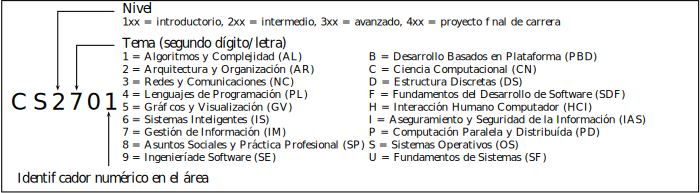
\includegraphics{/Users/ecuadros/Articles/Curricula/Curricula.Master/../Curricula.out/Peru/CS-MINEDU/cycle/2021-I/Plan2021/figs/course-coding}
   \caption{Esquema de codificaci\'on para los cursos.}
   \label{fig:course-number}
\end{figure}

El tipo de curso esta determinado por sus 2 primeras letras. Los posibles c\'odigos para estos tipos son:
\begin{enumerate}
\item \textbf{CS}  \'Area de Ciencia de la Computaci\'on (\textit{Computer Science});
\item \textbf{CB}  \'Area de Ciencias B\'asicas (F\'{i}­sica, Biolog\'{i}­a);
\item \textbf{MA}  Matem\'aticas (MA);
\item \textbf{FG}  \'Area de Formaci\'on General;
\item \textbf{ID}  \'Area de Idiomas.
\end{enumerate}



Al mismo tiempo, y de acuerdo a la ley universitaria vigente, los cursos est\'an clasificados en:
\begin{inparadesc}
\item [AF:] \'Area formativa,
\item [AE:] \'Area de especialidad,
\item [AB:] \'Area b\'asica,
\item [AC:] \'Area complementaria.
\end{inparadesc}


\section{Estructura Curricular}\label{sec:courses-by-semester}
La relaci\'on de cursos se muestra a continuaci\'on:
\begin{center}
\begin{tabular}{|l|l|c|c|c|c|c|c|p{6cm}|}
\multicolumn{9}{|l|}{\textbf{Primer Semestre}} \\  
\textbf{C\'odigo} & \textbf{Curso} & \textbf{\'Area} & \textbf{HT} & \textbf{HP} & \textbf{HL} & \textbf{Cr} & \textbf{TIPO} & \textbf{Requisitos} \\ 
\htmlref{\colorbox{cornflowerblue}{CS111}}{sec:CS111} & \htmlref{Introducci\'on a la Ciencia de la Computaci\'on}{sec:CS111} ~
\begin{htmlonly}
	\begin{rawhtml}
		<a href="syllabi/CS111-ES.pdf"> <img src="figs/pdf.jpeg" style="border: 0px solid ; width: 16px; height: 16px;"><img src="figs/ES.png" style="border: 0px solid ; width: 16px; height: 16px;"></a>,
		<a href="syllabi/CS111-EN.pdf"> <img src="figs/pdf.jpeg" style="border: 0px solid ; width: 16px; height: 16px;"><img src="figs/EN.png" style="border: 0px solid ; width: 16px; height: 16px;"></a>
	\end{rawhtml}
\end{htmlonly}
 & AF & 2 & ~ & 4 & 4 & O & ~ \\ 
\htmlref{\colorbox{cornflowerblue}{CS1D1}}{sec:CS1D1} & \htmlref{Estructuras Discretas I}{sec:CS1D1} ~
\begin{htmlonly}
	\begin{rawhtml}
		<a href="syllabi/CS1D1-ES.pdf"> <img src="figs/pdf.jpeg" style="border: 0px solid ; width: 16px; height: 16px;"><img src="figs/ES.png" style="border: 0px solid ; width: 16px; height: 16px;"></a>,
		<a href="syllabi/CS1D1-EN.pdf"> <img src="figs/pdf.jpeg" style="border: 0px solid ; width: 16px; height: 16px;"><img src="figs/EN.png" style="border: 0px solid ; width: 16px; height: 16px;"></a>
	\end{rawhtml}
\end{htmlonly}
 & AF & 2 & 4 & ~ & 4 & O & ~ \\ 
\htmlref{\colorbox{honeydew3}{MA100}}{sec:MA100} & \htmlref{Matem\'atica I}{sec:MA100} ~
\begin{htmlonly}
	\begin{rawhtml}
		<a href="syllabi/MA100-ES.pdf"> <img src="figs/pdf.jpeg" style="border: 0px solid ; width: 16px; height: 16px;"><img src="figs/ES.png" style="border: 0px solid ; width: 16px; height: 16px;"></a>,
		<a href="syllabi/MA100-EN.pdf"> <img src="figs/pdf.jpeg" style="border: 0px solid ; width: 16px; height: 16px;"><img src="figs/EN.png" style="border: 0px solid ; width: 16px; height: 16px;"></a>
	\end{rawhtml}
\end{htmlonly}
 & AB & 2 & 6 & ~ & 5 & O & ~ \\ 
\htmlref{\colorbox{chartreuse3}{FG101}}{sec:FG101} & \htmlref{Comunicaci\'on}{sec:FG101} ~
\begin{htmlonly}
	\begin{rawhtml}
		<a href="syllabi/FG101-ES.pdf"> <img src="figs/pdf.jpeg" style="border: 0px solid ; width: 16px; height: 16px;"><img src="figs/ES.png" style="border: 0px solid ; width: 16px; height: 16px;"></a>,
		<a href="syllabi/FG101-EN.pdf"> <img src="figs/pdf.jpeg" style="border: 0px solid ; width: 16px; height: 16px;"><img src="figs/EN.png" style="border: 0px solid ; width: 16px; height: 16px;"></a>
	\end{rawhtml}
\end{htmlonly}
 & AC & 2 & 2 & ~ & 3 & O & ~ \\ 
\htmlref{\colorbox{chartreuse3}{FG102}}{sec:FG102} & \htmlref{Metodolog\'{i}a del Estudio}{sec:FG102} ~
\begin{htmlonly}
	\begin{rawhtml}
		<a href="syllabi/FG102-ES.pdf"> <img src="figs/pdf.jpeg" style="border: 0px solid ; width: 16px; height: 16px;"><img src="figs/ES.png" style="border: 0px solid ; width: 16px; height: 16px;"></a>,
		<a href="syllabi/FG102-EN.pdf"> <img src="figs/pdf.jpeg" style="border: 0px solid ; width: 16px; height: 16px;"><img src="figs/EN.png" style="border: 0px solid ; width: 16px; height: 16px;"></a>
	\end{rawhtml}
\end{htmlonly}
 & AF & 2 & 2 & ~ & 3 & O & ~ \\ 
\htmlref{\colorbox{lightcoral}{ID101}}{sec:ID101} & \htmlref{Ingl\'es I}{sec:ID101} ~
\begin{htmlonly}
	\begin{rawhtml}
		<a href="syllabi/ID101-ES.pdf"> <img src="figs/pdf.jpeg" style="border: 0px solid ; width: 16px; height: 16px;"><img src="figs/ES.png" style="border: 0px solid ; width: 16px; height: 16px;"></a>,
		<a href="syllabi/ID101-EN.pdf"> <img src="figs/pdf.jpeg" style="border: 0px solid ; width: 16px; height: 16px;"><img src="figs/EN.png" style="border: 0px solid ; width: 16px; height: 16px;"></a>
	\end{rawhtml}
\end{htmlonly}
 & AC & ~ & 6 & ~ & 3 & O & ~ \\ 
\multicolumn{6}{l|}{} &  22 & \multicolumn{2}{|l}{} \\ \cline{7-7}
\end{tabular}
\end{center}

\begin{center}
\begin{tabular}{|l|l|c|c|c|c|c|c|p{6cm}|}
\multicolumn{9}{|l|}{\textbf{Segundo Semestre}} \\  
\textbf{C\'odigo} & \textbf{Curso} & \textbf{\'Area} & \textbf{HT} & \textbf{HP} & \textbf{HL} & \textbf{Cr} & \textbf{TIPO} & \textbf{Requisitos} \\ 
\htmlref{\colorbox{cornflowerblue}{CS112}}{sec:CS112} & \htmlref{Ciencia de la Computaci\'on I}{sec:CS112} ~
\begin{htmlonly}
	\begin{rawhtml}
		<a href="syllabi/CS112-ES.pdf"> <img src="figs/pdf.jpeg" style="border: 0px solid ; width: 16px; height: 16px;"><img src="figs/ES.png" style="border: 0px solid ; width: 16px; height: 16px;"></a>,
		<a href="syllabi/CS112-EN.pdf"> <img src="figs/pdf.jpeg" style="border: 0px solid ; width: 16px; height: 16px;"><img src="figs/EN.png" style="border: 0px solid ; width: 16px; height: 16px;"></a>
	\end{rawhtml}
\end{htmlonly}
 & AF & 2 & 2 & 4 & 5 & O & \htmlref{CS111}{sec:CS111} (1er~Sem) \\ 
\htmlref{\colorbox{cornflowerblue}{CS1D2}}{sec:CS1D2} & \htmlref{Estructuras Discretas II}{sec:CS1D2} ~
\begin{htmlonly}
	\begin{rawhtml}
		<a href="syllabi/CS1D2-ES.pdf"> <img src="figs/pdf.jpeg" style="border: 0px solid ; width: 16px; height: 16px;"><img src="figs/ES.png" style="border: 0px solid ; width: 16px; height: 16px;"></a>,
		<a href="syllabi/CS1D2-EN.pdf"> <img src="figs/pdf.jpeg" style="border: 0px solid ; width: 16px; height: 16px;"><img src="figs/EN.png" style="border: 0px solid ; width: 16px; height: 16px;"></a>
	\end{rawhtml}
\end{htmlonly}
 & AF & 2 & 2 & 2 & 4 & O & \htmlref{CS1D1}{sec:CS1D1} (1er~Sem) \\ 
\htmlref{\colorbox{honeydew3}{MA101}}{sec:MA101} & \htmlref{Matem\'atica II}{sec:MA101} ~
\begin{htmlonly}
	\begin{rawhtml}
		<a href="syllabi/MA101-ES.pdf"> <img src="figs/pdf.jpeg" style="border: 0px solid ; width: 16px; height: 16px;"><img src="figs/ES.png" style="border: 0px solid ; width: 16px; height: 16px;"></a>,
		<a href="syllabi/MA101-EN.pdf"> <img src="figs/pdf.jpeg" style="border: 0px solid ; width: 16px; height: 16px;"><img src="figs/EN.png" style="border: 0px solid ; width: 16px; height: 16px;"></a>
	\end{rawhtml}
\end{htmlonly}
 & AB & 2 & 4 & ~ & 4 & O & \htmlref{MA100}{sec:MA100} (1er~Sem) \\ 
\htmlref{\colorbox{chartreuse3}{FG106}}{sec:FG106} & \htmlref{Teatro}{sec:FG106} ~
\begin{htmlonly}
	\begin{rawhtml}
		<a href="syllabi/FG106-ES.pdf"> <img src="figs/pdf.jpeg" style="border: 0px solid ; width: 16px; height: 16px;"><img src="figs/ES.png" style="border: 0px solid ; width: 16px; height: 16px;"></a>,
		<a href="syllabi/FG106-EN.pdf"> <img src="figs/pdf.jpeg" style="border: 0px solid ; width: 16px; height: 16px;"><img src="figs/EN.png" style="border: 0px solid ; width: 16px; height: 16px;"></a>
	\end{rawhtml}
\end{htmlonly}
 & AC & 1 & 2 & ~ & 2 & O & \htmlref{FG101}{sec:FG101} (1er~Sem) \\ 
\htmlref{\colorbox{lightcoral}{ID102}}{sec:ID102} & \htmlref{Ingl\'es II}{sec:ID102} ~
\begin{htmlonly}
	\begin{rawhtml}
		<a href="syllabi/ID102-ES.pdf"> <img src="figs/pdf.jpeg" style="border: 0px solid ; width: 16px; height: 16px;"><img src="figs/ES.png" style="border: 0px solid ; width: 16px; height: 16px;"></a>,
		<a href="syllabi/ID102-EN.pdf"> <img src="figs/pdf.jpeg" style="border: 0px solid ; width: 16px; height: 16px;"><img src="figs/EN.png" style="border: 0px solid ; width: 16px; height: 16px;"></a>
	\end{rawhtml}
\end{htmlonly}
 & AC & 2 & 8 & ~ & 6 & O & \htmlref{ID101}{sec:ID101} (1er~Sem) \\ 
\multicolumn{6}{l|}{} &  21 & \multicolumn{2}{|l}{} \\ \cline{7-7}
\end{tabular}
\end{center}

\begin{center}
\begin{tabular}{|l|l|c|c|c|c|c|c|p{6cm}|}
\multicolumn{9}{|l|}{\textbf{Tercer Semestre}} \\  
\textbf{C\'odigo} & \textbf{Curso} & \textbf{\'Area} & \textbf{HT} & \textbf{HP} & \textbf{HL} & \textbf{Cr} & \textbf{TIPO} & \textbf{Requisitos} \\ 
\htmlref{\colorbox{cornflowerblue}{CS113}}{sec:CS113} & \htmlref{Ciencia de la Computaci\'on II}{sec:CS113} ~
\begin{htmlonly}
	\begin{rawhtml}
		<a href="syllabi/CS113-ES.pdf"> <img src="figs/pdf.jpeg" style="border: 0px solid ; width: 16px; height: 16px;"><img src="figs/ES.png" style="border: 0px solid ; width: 16px; height: 16px;"></a>,
		<a href="syllabi/CS113-EN.pdf"> <img src="figs/pdf.jpeg" style="border: 0px solid ; width: 16px; height: 16px;"><img src="figs/EN.png" style="border: 0px solid ; width: 16px; height: 16px;"></a>
	\end{rawhtml}
\end{htmlonly}
 & AF & 2 & ~ & 4 & 4 & O & \htmlref{CS112}{sec:CS112} (2do~Sem) \\ 
\htmlref{\colorbox{cornflowerblue}{CS221}}{sec:CS221} & \htmlref{Arquitectura de Computadores}{sec:CS221} ~
\begin{htmlonly}
	\begin{rawhtml}
		<a href="syllabi/CS221-ES.pdf"> <img src="figs/pdf.jpeg" style="border: 0px solid ; width: 16px; height: 16px;"><img src="figs/ES.png" style="border: 0px solid ; width: 16px; height: 16px;"></a>,
		<a href="syllabi/CS221-EN.pdf"> <img src="figs/pdf.jpeg" style="border: 0px solid ; width: 16px; height: 16px;"><img src="figs/EN.png" style="border: 0px solid ; width: 16px; height: 16px;"></a>
	\end{rawhtml}
\end{htmlonly}
 & AF & 2 & ~ & 2 & 3 & O & \htmlref{CS1D2}{sec:CS1D2} (2do~Sem) \\ 
\htmlref{\colorbox{cornflowerblue}{CS2B1}}{sec:CS2B1} & \htmlref{Desarrollo Basado en Plataformas}{sec:CS2B1} ~
\begin{htmlonly}
	\begin{rawhtml}
		<a href="syllabi/CS2B1-ES.pdf"> <img src="figs/pdf.jpeg" style="border: 0px solid ; width: 16px; height: 16px;"><img src="figs/ES.png" style="border: 0px solid ; width: 16px; height: 16px;"></a>,
		<a href="syllabi/CS2B1-EN.pdf"> <img src="figs/pdf.jpeg" style="border: 0px solid ; width: 16px; height: 16px;"><img src="figs/EN.png" style="border: 0px solid ; width: 16px; height: 16px;"></a>
	\end{rawhtml}
\end{htmlonly}
 & AF & 1 & 2 & 2 & 3 & O & \htmlref{CS112}{sec:CS112} (2do~Sem) \\ 
\htmlref{\colorbox{honeydew3}{MA203}}{sec:MA203} & \htmlref{Estad\'{i}stica y Probabilidades}{sec:MA203} ~
\begin{htmlonly}
	\begin{rawhtml}
		<a href="syllabi/MA203-ES.pdf"> <img src="figs/pdf.jpeg" style="border: 0px solid ; width: 16px; height: 16px;"><img src="figs/ES.png" style="border: 0px solid ; width: 16px; height: 16px;"></a>,
		<a href="syllabi/MA203-EN.pdf"> <img src="figs/pdf.jpeg" style="border: 0px solid ; width: 16px; height: 16px;"><img src="figs/EN.png" style="border: 0px solid ; width: 16px; height: 16px;"></a>
	\end{rawhtml}
\end{htmlonly}
 & AB & 2 & 2 & 2 & 4 & O & \htmlref{MA100}{sec:MA100} (1er~Sem) \\ 
\htmlref{\colorbox{chartreuse3}{FG203}}{sec:FG203} & \htmlref{Oratoria}{sec:FG203} ~
\begin{htmlonly}
	\begin{rawhtml}
		<a href="syllabi/FG203-ES.pdf"> <img src="figs/pdf.jpeg" style="border: 0px solid ; width: 16px; height: 16px;"><img src="figs/ES.png" style="border: 0px solid ; width: 16px; height: 16px;"></a>,
		<a href="syllabi/FG203-EN.pdf"> <img src="figs/pdf.jpeg" style="border: 0px solid ; width: 16px; height: 16px;"><img src="figs/EN.png" style="border: 0px solid ; width: 16px; height: 16px;"></a>
	\end{rawhtml}
\end{htmlonly}
 & AC & 1 & 2 & ~ & 2 & O & \htmlref{FG106}{sec:FG106} (2do~Sem) \\ 
\htmlref{\colorbox{lightcoral}{ID201}}{sec:ID201} & \htmlref{Ingl\'es III}{sec:ID201} ~
\begin{htmlonly}
	\begin{rawhtml}
		<a href="syllabi/ID201-ES.pdf"> <img src="figs/pdf.jpeg" style="border: 0px solid ; width: 16px; height: 16px;"><img src="figs/ES.png" style="border: 0px solid ; width: 16px; height: 16px;"></a>,
		<a href="syllabi/ID201-EN.pdf"> <img src="figs/pdf.jpeg" style="border: 0px solid ; width: 16px; height: 16px;"><img src="figs/EN.png" style="border: 0px solid ; width: 16px; height: 16px;"></a>
	\end{rawhtml}
\end{htmlonly}
 & AC & ~ & 6 & ~ & 3 & O & \htmlref{ID102}{sec:ID102} (2do~Sem) \\ 
\multicolumn{6}{l|}{} &  19 & \multicolumn{2}{|l}{} \\ \cline{7-7}
\end{tabular}
\end{center}

\begin{center}
\begin{tabular}{|l|l|c|c|c|c|c|c|p{6cm}|}
\multicolumn{9}{|l|}{\textbf{Cuarto Semestre}} \\  
\textbf{C\'odigo} & \textbf{Curso} & \textbf{\'Area} & \textbf{HT} & \textbf{HP} & \textbf{HL} & \textbf{Cr} & \textbf{TIPO} & \textbf{Requisitos} \\ 
\htmlref{\colorbox{cornflowerblue}{CS210}}{sec:CS210} & \htmlref{Algoritmos y Estructuras de Datos}{sec:CS210} ~
\begin{htmlonly}
	\begin{rawhtml}
		<a href="syllabi/CS210-ES.pdf"> <img src="figs/pdf.jpeg" style="border: 0px solid ; width: 16px; height: 16px;"><img src="figs/ES.png" style="border: 0px solid ; width: 16px; height: 16px;"></a>,
		<a href="syllabi/CS210-EN.pdf"> <img src="figs/pdf.jpeg" style="border: 0px solid ; width: 16px; height: 16px;"><img src="figs/EN.png" style="border: 0px solid ; width: 16px; height: 16px;"></a>
	\end{rawhtml}
\end{htmlonly}
 & AF & 2 & 2 & 2 & 4 & O & \htmlref{CS113}{sec:CS113} (3er~Sem) \\ 
\htmlref{\colorbox{cornflowerblue}{CS211}}{sec:CS211} & \htmlref{Teor\'{i}a de la Computaci\'on}{sec:CS211} ~
\begin{htmlonly}
	\begin{rawhtml}
		<a href="syllabi/CS211-ES.pdf"> <img src="figs/pdf.jpeg" style="border: 0px solid ; width: 16px; height: 16px;"><img src="figs/ES.png" style="border: 0px solid ; width: 16px; height: 16px;"></a>,
		<a href="syllabi/CS211-EN.pdf"> <img src="figs/pdf.jpeg" style="border: 0px solid ; width: 16px; height: 16px;"><img src="figs/EN.png" style="border: 0px solid ; width: 16px; height: 16px;"></a>
	\end{rawhtml}
\end{htmlonly}
 & AF & 2 & 2 & 2 & 4 & O & \htmlref{CS1D2}{sec:CS1D2} (2do~Sem) \\ 
\htmlref{\colorbox{cornflowerblue}{CS271}}{sec:CS271} & \htmlref{Gerenciamiento de Datos I}{sec:CS271} ~
\begin{htmlonly}
	\begin{rawhtml}
		<a href="syllabi/CS271-ES.pdf"> <img src="figs/pdf.jpeg" style="border: 0px solid ; width: 16px; height: 16px;"><img src="figs/ES.png" style="border: 0px solid ; width: 16px; height: 16px;"></a>,
		<a href="syllabi/CS271-EN.pdf"> <img src="figs/pdf.jpeg" style="border: 0px solid ; width: 16px; height: 16px;"><img src="figs/EN.png" style="border: 0px solid ; width: 16px; height: 16px;"></a>
	\end{rawhtml}
\end{htmlonly}
 & AF & 2 & ~ & 4 & 4 & O & \htmlref{CS112}{sec:CS112} (2do~Sem),\htmlref{CS1D2}{sec:CS1D2} (2do~Sem) \\ 
\htmlref{\colorbox{cornflowerblue}{CS2S1}}{sec:CS2S1} & \htmlref{Sistemas Operativos}{sec:CS2S1} ~
\begin{htmlonly}
	\begin{rawhtml}
		<a href="syllabi/CS2S1-ES.pdf"> <img src="figs/pdf.jpeg" style="border: 0px solid ; width: 16px; height: 16px;"><img src="figs/ES.png" style="border: 0px solid ; width: 16px; height: 16px;"></a>,
		<a href="syllabi/CS2S1-EN.pdf"> <img src="figs/pdf.jpeg" style="border: 0px solid ; width: 16px; height: 16px;"><img src="figs/EN.png" style="border: 0px solid ; width: 16px; height: 16px;"></a>
	\end{rawhtml}
\end{htmlonly}
 & AF & 2 & 2 & 2 & 4 & O & \htmlref{CS221}{sec:CS221} (3er~Sem) \\ 
\htmlref{\colorbox{chartreuse3}{FG350}}{sec:FG350} & \htmlref{Liderazgo y Desempe\~no}{sec:FG350} ~
\begin{htmlonly}
	\begin{rawhtml}
		<a href="syllabi/FG350-ES.pdf"> <img src="figs/pdf.jpeg" style="border: 0px solid ; width: 16px; height: 16px;"><img src="figs/ES.png" style="border: 0px solid ; width: 16px; height: 16px;"></a>,
		<a href="syllabi/FG350-EN.pdf"> <img src="figs/pdf.jpeg" style="border: 0px solid ; width: 16px; height: 16px;"><img src="figs/EN.png" style="border: 0px solid ; width: 16px; height: 16px;"></a>
	\end{rawhtml}
\end{htmlonly}
 & AC & 2 & ~ & ~ & 2 & O & \htmlref{FG203}{sec:FG203} (3er~Sem) \\ 
\htmlref{\colorbox{lightcoral}{ID202}}{sec:ID202} & \htmlref{Ingl\'es IV}{sec:ID202} ~
\begin{htmlonly}
	\begin{rawhtml}
		<a href="syllabi/ID202-ES.pdf"> <img src="figs/pdf.jpeg" style="border: 0px solid ; width: 16px; height: 16px;"><img src="figs/ES.png" style="border: 0px solid ; width: 16px; height: 16px;"></a>,
		<a href="syllabi/ID202-EN.pdf"> <img src="figs/pdf.jpeg" style="border: 0px solid ; width: 16px; height: 16px;"><img src="figs/EN.png" style="border: 0px solid ; width: 16px; height: 16px;"></a>
	\end{rawhtml}
\end{htmlonly}
 & AC & ~ & 10 & ~ & 3 & O & \htmlref{ID201}{sec:ID201} (3er~Sem) \\ 
\multicolumn{6}{l|}{} &  21 & \multicolumn{2}{|l}{} \\ \cline{7-7}
\end{tabular}
\end{center}

\begin{center}
\begin{tabular}{|l|l|c|c|c|c|c|c|p{6cm}|}
\multicolumn{9}{|l|}{\textbf{Quinto Semestre}} \\  
\textbf{C\'odigo} & \textbf{Curso} & \textbf{\'Area} & \textbf{HT} & \textbf{HP} & \textbf{HL} & \textbf{Cr} & \textbf{TIPO} & \textbf{Requisitos} \\ 
\htmlref{\colorbox{cornflowerblue}{CS212}}{sec:CS212} & \htmlref{An\'alisis y Dise\~no de Algoritmos}{sec:CS212} ~
\begin{htmlonly}
	\begin{rawhtml}
		<a href="syllabi/CS212-ES.pdf"> <img src="figs/pdf.jpeg" style="border: 0px solid ; width: 16px; height: 16px;"><img src="figs/ES.png" style="border: 0px solid ; width: 16px; height: 16px;"></a>,
		<a href="syllabi/CS212-EN.pdf"> <img src="figs/pdf.jpeg" style="border: 0px solid ; width: 16px; height: 16px;"><img src="figs/EN.png" style="border: 0px solid ; width: 16px; height: 16px;"></a>
	\end{rawhtml}
\end{htmlonly}
 & AF & 2 & ~ & 4 & 4 & O & \htmlref{CS210}{sec:CS210} (4to~Sem),\htmlref{CS211}{sec:CS211} (4to~Sem) \\ 
\htmlref{\colorbox{cornflowerblue}{CS231}}{sec:CS231} & \htmlref{Redes y Comunicaciones}{sec:CS231} ~
\begin{htmlonly}
	\begin{rawhtml}
		<a href="syllabi/CS231-ES.pdf"> <img src="figs/pdf.jpeg" style="border: 0px solid ; width: 16px; height: 16px;"><img src="figs/ES.png" style="border: 0px solid ; width: 16px; height: 16px;"></a>,
		<a href="syllabi/CS231-EN.pdf"> <img src="figs/pdf.jpeg" style="border: 0px solid ; width: 16px; height: 16px;"><img src="figs/EN.png" style="border: 0px solid ; width: 16px; height: 16px;"></a>
	\end{rawhtml}
\end{htmlonly}
 & AE & 1 & ~ & 4 & 3 & O & \htmlref{CS2S1}{sec:CS2S1} (4to~Sem) \\ 
\htmlref{\colorbox{cornflowerblue}{CS261}}{sec:CS261} & \htmlref{Sistemas Inteligentes}{sec:CS261} ~
\begin{htmlonly}
	\begin{rawhtml}
		<a href="syllabi/CS261-ES.pdf"> <img src="figs/pdf.jpeg" style="border: 0px solid ; width: 16px; height: 16px;"><img src="figs/ES.png" style="border: 0px solid ; width: 16px; height: 16px;"></a>,
		<a href="syllabi/CS261-EN.pdf"> <img src="figs/pdf.jpeg" style="border: 0px solid ; width: 16px; height: 16px;"><img src="figs/EN.png" style="border: 0px solid ; width: 16px; height: 16px;"></a>
	\end{rawhtml}
\end{htmlonly}
 & AF & 2 & 2 & 2 & 4 & O & \htmlref{MA203}{sec:MA203} (3er~Sem) \\ 
\htmlref{\colorbox{cornflowerblue}{CS291}}{sec:CS291} & \htmlref{Ingenier\'{i}a de Software I}{sec:CS291} ~
\begin{htmlonly}
	\begin{rawhtml}
		<a href="syllabi/CS291-ES.pdf"> <img src="figs/pdf.jpeg" style="border: 0px solid ; width: 16px; height: 16px;"><img src="figs/ES.png" style="border: 0px solid ; width: 16px; height: 16px;"></a>,
		<a href="syllabi/CS291-EN.pdf"> <img src="figs/pdf.jpeg" style="border: 0px solid ; width: 16px; height: 16px;"><img src="figs/EN.png" style="border: 0px solid ; width: 16px; height: 16px;"></a>
	\end{rawhtml}
\end{htmlonly}
 & AF & 2 & 2 & 2 & 4 & O & \htmlref{CS113}{sec:CS113} (3er~Sem),\htmlref{CS271}{sec:CS271} (4to~Sem) \\ 
\htmlref{\colorbox{cornflowerblue}{CS2H1}}{sec:CS2H1} & \htmlref{Experiencia de Usuario  (UX)}{sec:CS2H1} ~
\begin{htmlonly}
	\begin{rawhtml}
		<a href="syllabi/CS2H1-ES.pdf"> <img src="figs/pdf.jpeg" style="border: 0px solid ; width: 16px; height: 16px;"><img src="figs/ES.png" style="border: 0px solid ; width: 16px; height: 16px;"></a>,
		<a href="syllabi/CS2H1-EN.pdf"> <img src="figs/pdf.jpeg" style="border: 0px solid ; width: 16px; height: 16px;"><img src="figs/EN.png" style="border: 0px solid ; width: 16px; height: 16px;"></a>
	\end{rawhtml}
\end{htmlonly}
 & AE & 1 & ~ & 4 & 3 & O & \htmlref{CS113}{sec:CS113} (3er~Sem) \\ 
\htmlref{\colorbox{honeydew3}{CB111}}{sec:CB111} & \htmlref{F\'{i}sica Computacional}{sec:CB111} ~
\begin{htmlonly}
	\begin{rawhtml}
		<a href="syllabi/CB111-ES.pdf"> <img src="figs/pdf.jpeg" style="border: 0px solid ; width: 16px; height: 16px;"><img src="figs/ES.png" style="border: 0px solid ; width: 16px; height: 16px;"></a>,
		<a href="syllabi/CB111-EN.pdf"> <img src="figs/pdf.jpeg" style="border: 0px solid ; width: 16px; height: 16px;"><img src="figs/EN.png" style="border: 0px solid ; width: 16px; height: 16px;"></a>
	\end{rawhtml}
\end{htmlonly}
 & AB & 2 & 2 & 2 & 4 & O & \htmlref{MA100}{sec:MA100} (1er~Sem) \\ 
\htmlref{\colorbox{lightcoral}{ID203}}{sec:ID203} & \htmlref{Ingl\'es V}{sec:ID203} ~
\begin{htmlonly}
	\begin{rawhtml}
		<a href="syllabi/ID203-ES.pdf"> <img src="figs/pdf.jpeg" style="border: 0px solid ; width: 16px; height: 16px;"><img src="figs/ES.png" style="border: 0px solid ; width: 16px; height: 16px;"></a>,
		<a href="syllabi/ID203-EN.pdf"> <img src="figs/pdf.jpeg" style="border: 0px solid ; width: 16px; height: 16px;"><img src="figs/EN.png" style="border: 0px solid ; width: 16px; height: 16px;"></a>
	\end{rawhtml}
\end{htmlonly}
 & AC & 2 & 2 & ~ & 3 & O & \htmlref{ID202}{sec:ID202} (4to~Sem) \\ 
\multicolumn{6}{l|}{} &  25 & \multicolumn{2}{|l}{} \\ \cline{7-7}
\end{tabular}
\end{center}

\begin{center}
\begin{tabular}{|l|l|c|c|c|c|c|c|p{6cm}|}
\multicolumn{9}{|l|}{\textbf{Sexto Semestre}} \\  
\textbf{C\'odigo} & \textbf{Curso} & \textbf{\'Area} & \textbf{HT} & \textbf{HP} & \textbf{HL} & \textbf{Cr} & \textbf{TIPO} & \textbf{Requisitos} \\ 
\htmlref{\colorbox{cornflowerblue}{CS292}}{sec:CS292} & \htmlref{Ingenier\'{i}a de Software II}{sec:CS292} ~
\begin{htmlonly}
	\begin{rawhtml}
		<a href="syllabi/CS292-ES.pdf"> <img src="figs/pdf.jpeg" style="border: 0px solid ; width: 16px; height: 16px;"><img src="figs/ES.png" style="border: 0px solid ; width: 16px; height: 16px;"></a>,
		<a href="syllabi/CS292-EN.pdf"> <img src="figs/pdf.jpeg" style="border: 0px solid ; width: 16px; height: 16px;"><img src="figs/EN.png" style="border: 0px solid ; width: 16px; height: 16px;"></a>
	\end{rawhtml}
\end{htmlonly}
 & AF & 2 & 2 & 2 & 4 & O & \htmlref{CS291}{sec:CS291} (5to~Sem) \\ 
\htmlref{\colorbox{cornflowerblue}{CS311}}{sec:CS311} & \htmlref{Programaci\'on Competitiva}{sec:CS311} ~
\begin{htmlonly}
	\begin{rawhtml}
		<a href="syllabi/CS311-ES.pdf"> <img src="figs/pdf.jpeg" style="border: 0px solid ; width: 16px; height: 16px;"><img src="figs/ES.png" style="border: 0px solid ; width: 16px; height: 16px;"></a>,
		<a href="syllabi/CS311-EN.pdf"> <img src="figs/pdf.jpeg" style="border: 0px solid ; width: 16px; height: 16px;"><img src="figs/EN.png" style="border: 0px solid ; width: 16px; height: 16px;"></a>
	\end{rawhtml}
\end{htmlonly}
 & FG & 2 & 2 & 2 & 4 & O & \htmlref{CS212}{sec:CS212} (5to~Sem) \\ 
\htmlref{\colorbox{cornflowerblue}{CS312}}{sec:CS312} & \htmlref{Estructuras de Datos Avanzadas}{sec:CS312} ~
\begin{htmlonly}
	\begin{rawhtml}
		<a href="syllabi/CS312-ES.pdf"> <img src="figs/pdf.jpeg" style="border: 0px solid ; width: 16px; height: 16px;"><img src="figs/ES.png" style="border: 0px solid ; width: 16px; height: 16px;"></a>,
		<a href="syllabi/CS312-EN.pdf"> <img src="figs/pdf.jpeg" style="border: 0px solid ; width: 16px; height: 16px;"><img src="figs/EN.png" style="border: 0px solid ; width: 16px; height: 16px;"></a>
	\end{rawhtml}
\end{htmlonly}
 & AF & 2 & 2 & 2 & 4 & O & \htmlref{CS212}{sec:CS212} (5to~Sem) \\ 
\htmlref{\colorbox{cornflowerblue}{CS393}}{sec:CS393} & \htmlref{Sistemas de Infomaci\'on}{sec:CS393} ~
\begin{htmlonly}
	\begin{rawhtml}
		<a href="syllabi/CS393-ES.pdf"> <img src="figs/pdf.jpeg" style="border: 0px solid ; width: 16px; height: 16px;"><img src="figs/ES.png" style="border: 0px solid ; width: 16px; height: 16px;"></a>,
		<a href="syllabi/CS393-EN.pdf"> <img src="figs/pdf.jpeg" style="border: 0px solid ; width: 16px; height: 16px;"><img src="figs/EN.png" style="border: 0px solid ; width: 16px; height: 16px;"></a>
	\end{rawhtml}
\end{htmlonly}
 & AE & 2 & 2 & 2 & 4 & O & \htmlref{CS291}{sec:CS291} (5to~Sem) \\ 
\htmlref{\colorbox{cornflowerblue}{CS3I1}}{sec:CS3I1} & \htmlref{Seguridad en Computaci\'on}{sec:CS3I1} ~
\begin{htmlonly}
	\begin{rawhtml}
		<a href="syllabi/CS3I1-ES.pdf"> <img src="figs/pdf.jpeg" style="border: 0px solid ; width: 16px; height: 16px;"><img src="figs/ES.png" style="border: 0px solid ; width: 16px; height: 16px;"></a>,
		<a href="syllabi/CS3I1-EN.pdf"> <img src="figs/pdf.jpeg" style="border: 0px solid ; width: 16px; height: 16px;"><img src="figs/EN.png" style="border: 0px solid ; width: 16px; height: 16px;"></a>
	\end{rawhtml}
\end{htmlonly}
 & AE & 1 & ~ & 4 & 3 & O & \htmlref{CS231}{sec:CS231} (5to~Sem) \\ 
\htmlref{\colorbox{cornflowerblue}{CS3P1}}{sec:CS3P1} & \htmlref{Computaci\'on Paralela y Distribu\'{i}da}{sec:CS3P1} ~
\begin{htmlonly}
	\begin{rawhtml}
		<a href="syllabi/CS3P1-ES.pdf"> <img src="figs/pdf.jpeg" style="border: 0px solid ; width: 16px; height: 16px;"><img src="figs/ES.png" style="border: 0px solid ; width: 16px; height: 16px;"></a>,
		<a href="syllabi/CS3P1-EN.pdf"> <img src="figs/pdf.jpeg" style="border: 0px solid ; width: 16px; height: 16px;"><img src="figs/EN.png" style="border: 0px solid ; width: 16px; height: 16px;"></a>
	\end{rawhtml}
\end{htmlonly}
 & AF & 2 & ~ & 4 & 4 & O & \htmlref{CS212}{sec:CS212} (5to~Sem),\htmlref{CS231}{sec:CS231} (5to~Sem) \\ 
\htmlref{\colorbox{lightcoral}{ID204}}{sec:ID204} & \htmlref{Ingl\'es VI}{sec:ID204} ~
\begin{htmlonly}
	\begin{rawhtml}
		<a href="syllabi/ID204-ES.pdf"> <img src="figs/pdf.jpeg" style="border: 0px solid ; width: 16px; height: 16px;"><img src="figs/ES.png" style="border: 0px solid ; width: 16px; height: 16px;"></a>,
		<a href="syllabi/ID204-EN.pdf"> <img src="figs/pdf.jpeg" style="border: 0px solid ; width: 16px; height: 16px;"><img src="figs/EN.png" style="border: 0px solid ; width: 16px; height: 16px;"></a>
	\end{rawhtml}
\end{htmlonly}
 & AC & 2 & 2 & ~ & 3 & O & \htmlref{ID203}{sec:ID203} (5to~Sem) \\ 
\multicolumn{6}{l|}{} &  26 & \multicolumn{2}{|l}{} \\ \cline{7-7}
\end{tabular}
\end{center}

\noindent\textbf{Total de cr\'editos de la carrera: } 134 
.




\section{Distribuci\'on de t\'opicos por curso}\label{sec:topics-by-course}
Las siguientes tablas nos muestran la distribuci\'on de todos los t\'opicos del 
cuerpo del conocimiento de \ac{CS} en todos los cursos.
\begin{center}
\begin{table}[H]
\begin{tabular}{|c|l|c|c|c|c|c|c|c|c|c|c|c|c|} 
 & & \multicolumn{6}{c}{Primer Sem} & \multicolumn{5}{c}{Segundo Sem} & . \\ 
 ~ & \textbf{Unidades de Conocimiento} & \colorbox{cornflowerblue}{\htmlref{CS111}{sec:CS111}} & \colorbox{cornflowerblue}{\htmlref{CS1D1}{sec:CS1D1}} & \colorbox{honeydew3}{\htmlref{MA100}{sec:MA100}} & \colorbox{chartreuse3}{\htmlref{FG101}{sec:FG101}} & \colorbox{chartreuse3}{\htmlref{FG102}{sec:FG102}} & \colorbox{lightcoral}{\htmlref{ID101}{sec:ID101}} & \colorbox{cornflowerblue}{\htmlref{CS112}{sec:CS112}} & \colorbox{cornflowerblue}{\htmlref{CS1D2}{sec:CS1D2}} & \colorbox{honeydew3}{\htmlref{MA101}{sec:MA101}} & \colorbox{chartreuse3}{\htmlref{FG106}{sec:FG106}} & \colorbox{lightcoral}{\htmlref{ID102}{sec:ID102}} & Total \\ 
 	\latexhtml{$\bigstar$}{}
	\begin{htmlonly}
		\begin{rawhtml}
			<img src="./figs/star.gif" style="border: 0px solid ; width: 16px; height: 16px;">
		\end{rawhtml}
	\end{htmlonly}
 & \htmlref{AL An\'alisis B\'asico  (2 horas Core-Tier1,~2 horas Core-Tier2)}{sec:BOK:ALBasicAnalysis} & \htmlref{2}{sec:CS111} & ~ & ~ & ~ & ~ & ~ & \htmlref{2}{sec:CS112} & ~ & ~ & ~ & ~ & 4 \\ 
 	\latexhtml{$\bigstar$}{}
	\begin{htmlonly}
		\begin{rawhtml}
			<img src="./figs/star.gif" style="border: 0px solid ; width: 16px; height: 16px;">
		\end{rawhtml}
	\end{htmlonly}
 & \htmlref{AL Estrategias Algor\'{i}tmicas  (5 horas Core-Tier1,~1 horas Core-Tier2)}{sec:BOK:ALAlgorithmicStrategies} & ~ & ~ & ~ & ~ & ~ & ~ & \htmlref{3}{sec:CS112} & ~ & ~ & ~ & ~ & 3 \\ 
 	\latexhtml{$\bigstar$}{}
	\begin{htmlonly}
		\begin{rawhtml}
			<img src="./figs/star.gif" style="border: 0px solid ; width: 16px; height: 16px;">
		\end{rawhtml}
	\end{htmlonly}
 & \htmlref{AL Algoritmos y Estructuras de Datos fundamentales  (9 horas Core-Tier1,~3 horas Core-Tier2)}{sec:BOK:ALFundamentalDataStructuresandAlgorithms} & \htmlref{8}{sec:CS111} & ~ & ~ & ~ & ~ & ~ & \htmlref{6}{sec:CS112} & ~ & ~ & ~ & ~ & 14 \\ 
 	\latexhtml{$\bigstar$}{}
	\begin{htmlonly}
		\begin{rawhtml}
			<img src="./figs/star.gif" style="border: 0px solid ; width: 16px; height: 16px;">
		\end{rawhtml}
	\end{htmlonly}
 & \htmlref{DS Funciones, relaciones y conjuntos  (4 horas Core-Tier1)}{sec:BOK:DSSetsRelationsandFunctions} & ~ & \htmlref{22}{sec:CS1D1} & ~ & ~ & ~ & ~ & ~ & ~ & ~ & ~ & ~ & 22 \\ 
 	\latexhtml{$\bigstar$}{}
	\begin{htmlonly}
		\begin{rawhtml}
			<img src="./figs/star.gif" style="border: 0px solid ; width: 16px; height: 16px;">
		\end{rawhtml}
	\end{htmlonly}
 & \htmlref{DS L\'ogica b\'asica  (9 horas Core-Tier1)}{sec:BOK:DSBasicLogic} & ~ & \htmlref{14}{sec:CS1D1} & ~ & ~ & ~ & ~ & ~ & ~ & ~ & ~ & ~ & 14 \\ 
 	\latexhtml{$\bigstar$}{}
	\begin{htmlonly}
		\begin{rawhtml}
			<img src="./figs/star.gif" style="border: 0px solid ; width: 16px; height: 16px;">
		\end{rawhtml}
	\end{htmlonly}
 & \htmlref{DS T\'ecnicas de demostraci\'on  (10 horas Core-Tier1,~1 horas Core-Tier2)}{sec:BOK:DSProofTechniques} & ~ & \htmlref{14}{sec:CS1D1} & ~ & ~ & ~ & ~ & ~ & ~ & ~ & ~ & ~ & 14 \\ 
 	\latexhtml{$\bigstar$}{}
	\begin{htmlonly}
		\begin{rawhtml}
			<img src="./figs/star.gif" style="border: 0px solid ; width: 16px; height: 16px;">
		\end{rawhtml}
	\end{htmlonly}
 & \htmlref{DS Fundamentos de conteo  (5 horas Core-Tier1)}{sec:BOK:DSBasicsofCounting} & ~ & ~ & ~ & ~ & ~ & ~ & ~ & \htmlref{40}{sec:CS1D2} & ~ & ~ & ~ & 40 \\ 
 	\latexhtml{$\bigstar$}{}
	\begin{htmlonly}
		\begin{rawhtml}
			<img src="./figs/star.gif" style="border: 0px solid ; width: 16px; height: 16px;">
		\end{rawhtml}
	\end{htmlonly}
 & \htmlref{DS \'Arboles y Grafos  (3 horas Core-Tier1,~1 horas Core-Tier2)}{sec:BOK:DSGraphsandTrees} & ~ & ~ & ~ & ~ & ~ & ~ & ~ & \htmlref{40}{sec:CS1D2} & ~ & ~ & ~ & 40 \\ 
 	\latexhtml{$\bigstar$}{}
	\begin{htmlonly}
		\begin{rawhtml}
			<img src="./figs/star.gif" style="border: 0px solid ; width: 16px; height: 16px;">
		\end{rawhtml}
	\end{htmlonly}
 & \htmlref{PL Programaci\'on orientada a objetos  (4 horas Core-Tier1,~6 horas Core-Tier2)}{sec:BOK:PLObjectOrientedProgramming} & ~ & ~ & ~ & ~ & ~ & ~ & \htmlref{10}{sec:CS112} & ~ & ~ & ~ & ~ & 10 \\ 
 	\latexhtml{$\bigstar$}{}
	\begin{htmlonly}
		\begin{rawhtml}
			<img src="./figs/star.gif" style="border: 0px solid ; width: 16px; height: 16px;">
		\end{rawhtml}
	\end{htmlonly}
 & \htmlref{PL Sistemas de tipos b\'asicos  (1 horas Core-Tier1,~4 horas Core-Tier2)}{sec:BOK:PLBasicTypeSystems} & \htmlref{2}{sec:CS111} & ~ & ~ & ~ & ~ & ~ & \htmlref{2}{sec:CS112} & ~ & ~ & ~ & ~ & 4 \\ 
 	\latexhtml{$\bigstar$}{}
	\begin{htmlonly}
		\begin{rawhtml}
			<img src="./figs/star.gif" style="border: 0px solid ; width: 16px; height: 16px;">
		\end{rawhtml}
	\end{htmlonly}
 & \htmlref{SDF Algoritmos y Dise\~no  (11 horas Core-Tier1)}{sec:BOK:SDFAlgorithmsandDesign} & \htmlref{9}{sec:CS111} & ~ & ~ & ~ & ~ & ~ & \htmlref{3}{sec:CS112} & ~ & ~ & ~ & ~ & 12 \\ 
 	\latexhtml{$\bigstar$}{}
	\begin{htmlonly}
		\begin{rawhtml}
			<img src="./figs/star.gif" style="border: 0px solid ; width: 16px; height: 16px;">
		\end{rawhtml}
	\end{htmlonly}
 & \htmlref{SDF Conceptos Fundamentales de Programaci\'on  (10 horas Core-Tier1)}{sec:BOK:SDFFundamentalProgrammingConcepts} & \htmlref{9}{sec:CS111} & ~ & ~ & ~ & ~ & ~ & \htmlref{6}{sec:CS112} & ~ & ~ & ~ & ~ & 15 \\ 
 	\latexhtml{$\bigstar$}{}
	\begin{htmlonly}
		\begin{rawhtml}
			<img src="./figs/star.gif" style="border: 0px solid ; width: 16px; height: 16px;">
		\end{rawhtml}
	\end{htmlonly}
 & \htmlref{SDF M\'etodos de Desarrollo  (10 horas Core-Tier1)}{sec:BOK:SDFDevelopmentMethods} & \htmlref{1}{sec:CS111} & ~ & ~ & ~ & ~ & ~ & ~ & ~ & ~ & ~ & ~ & 1 \\ 
 	\latexhtml{~}{}
	\begin{htmlonly}
		\begin{rawhtml}
			<img src="./figs/none.gif" style="border: 0px solid ; width: 16px; height: 16px;">
		\end{rawhtml}
	\end{htmlonly}
 & \htmlref{SP Historia }{sec:BOK:SPHistory} & \htmlref{5}{sec:CS111} & ~ & ~ & ~ & ~ & ~ & ~ & ~ & ~ & ~ & ~ & 5 \\ 
~ & Total & 36 & 50 & 0 & 0 & 0 & 0 & 32 & 80 & 0 & 0 & 0 &        \\ 
\end{tabular}
\caption{T\'opicos por curso del 1er al 2do Semestre}
\end{table}
\end{center}

\begin{center}
\begin{table}[H]
\begin{tabular}{|c|l|c|c|c|c|c|c|c|c|c|c|c|c|c|} 
 & & \multicolumn{6}{c}{Tercer Sem} & \multicolumn{6}{c}{Cuarto Sem} & . \\ 
 ~ & \textbf{Unidades de Conocimiento} & \colorbox{cornflowerblue}{\htmlref{CS113}{sec:CS113}} & \colorbox{cornflowerblue}{\htmlref{CS221}{sec:CS221}} & \colorbox{cornflowerblue}{\htmlref{CS2B1}{sec:CS2B1}} & \colorbox{honeydew3}{\htmlref{MA203}{sec:MA203}} & \colorbox{chartreuse3}{\htmlref{FG203}{sec:FG203}} & \colorbox{lightcoral}{\htmlref{ID201}{sec:ID201}} & \colorbox{cornflowerblue}{\htmlref{CS210}{sec:CS210}} & \colorbox{cornflowerblue}{\htmlref{CS211}{sec:CS211}} & \colorbox{cornflowerblue}{\htmlref{CS271}{sec:CS271}} & \colorbox{cornflowerblue}{\htmlref{CS2S1}{sec:CS2S1}} & \colorbox{chartreuse3}{\htmlref{FG350}{sec:FG350}} & \colorbox{lightcoral}{\htmlref{ID202}{sec:ID202}} & Total \\ 
 	\latexhtml{$\bigstar$}{}
	\begin{htmlonly}
		\begin{rawhtml}
			<img src="./figs/star.gif" style="border: 0px solid ; width: 16px; height: 16px;">
		\end{rawhtml}
	\end{htmlonly}
 & \htmlref{AL An\'alisis B\'asico  (2 horas Core-Tier1,~2 horas Core-Tier2)}{sec:BOK:ALBasicAnalysis} & \htmlref{3}{sec:CS113} & ~ & ~ & ~ & ~ & ~ & ~ & ~ & ~ & ~ & ~ & ~ & 3 \\ 
 	\latexhtml{$\bigstar$}{}
	\begin{htmlonly}
		\begin{rawhtml}
			<img src="./figs/star.gif" style="border: 0px solid ; width: 16px; height: 16px;">
		\end{rawhtml}
	\end{htmlonly}
 & \htmlref{AL Algoritmos y Estructuras de Datos fundamentales  (9 horas Core-Tier1,~3 horas Core-Tier2)}{sec:BOK:ALFundamentalDataStructuresandAlgorithms} & \htmlref{3}{sec:CS113} & ~ & ~ & ~ & ~ & ~ & ~ & ~ & ~ & ~ & ~ & ~ & 3 \\ 
 	\latexhtml{$\bigstar$}{}
	\begin{htmlonly}
		\begin{rawhtml}
			<img src="./figs/star.gif" style="border: 0px solid ; width: 16px; height: 16px;">
		\end{rawhtml}
	\end{htmlonly}
 & \htmlref{AL Computabilidad y complejidad b\'asica de aut\'omatas  (3 horas Core-Tier1,~3 horas Core-Tier2)}{sec:BOK:ALBasicAutomataComputabilityandComplexity} & ~ & ~ & ~ & ~ & ~ & ~ & ~ & \htmlref{20}{sec:CS211} & ~ & ~ & ~ & ~ & 20 \\ 
 	\latexhtml{~}{}
	\begin{htmlonly}
		\begin{rawhtml}
			<img src="./figs/none.gif" style="border: 0px solid ; width: 16px; height: 16px;">
		\end{rawhtml}
	\end{htmlonly}
 & \htmlref{AL Complejidad Computacional Avanzada }{sec:BOK:ALAdvancedComputationalComplexity} & ~ & ~ & ~ & ~ & ~ & ~ & ~ & \htmlref{20}{sec:CS211} & ~ & ~ & ~ & ~ & 20 \\ 
 	\latexhtml{~}{}
	\begin{htmlonly}
		\begin{rawhtml}
			<img src="./figs/none.gif" style="border: 0px solid ; width: 16px; height: 16px;">
		\end{rawhtml}
	\end{htmlonly}
 & \htmlref{AL Teor\'{i}a y Computabilidad Avanzada de Aut\'omatas }{sec:BOK:ALAdvancedAutomataTheoryandComputability} & ~ & ~ & ~ & ~ & ~ & ~ & ~ & \htmlref{20}{sec:CS211} & ~ & ~ & ~ & ~ & 20 \\ 
 	\latexhtml{$\bigstar$}{}
	\begin{htmlonly}
		\begin{rawhtml}
			<img src="./figs/star.gif" style="border: 0px solid ; width: 16px; height: 16px;">
		\end{rawhtml}
	\end{htmlonly}
 & \htmlref{AR L\'ogica digital y sistemas digitales  (3 horas Core-Tier2)}{sec:BOK:ARDigitallogicanddigitalsystems} & ~ & \htmlref{18}{sec:CS221} & ~ & ~ & ~ & ~ & ~ & ~ & ~ & ~ & ~ & ~ & 18 \\ 
 	\latexhtml{$\bigstar$}{}
	\begin{htmlonly}
		\begin{rawhtml}
			<img src="./figs/star.gif" style="border: 0px solid ; width: 16px; height: 16px;">
		\end{rawhtml}
	\end{htmlonly}
 & \htmlref{AR Representaci\'on de datos a nivel m\'aquina  (3 horas Core-Tier2)}{sec:BOK:ARMachinelevelrepresentationofdata} & ~ & \htmlref{8}{sec:CS221} & ~ & ~ & ~ & ~ & ~ & ~ & ~ & ~ & ~ & ~ & 8 \\ 
 	\latexhtml{$\bigstar$}{}
	\begin{htmlonly}
		\begin{rawhtml}
			<img src="./figs/star.gif" style="border: 0px solid ; width: 16px; height: 16px;">
		\end{rawhtml}
	\end{htmlonly}
 & \htmlref{AR Organizaci\'on de la M\'aquina a Nivel Ensamblador  (6 horas Core-Tier2)}{sec:BOK:ARAssemblylevelmachineorganization} & ~ & \htmlref{8}{sec:CS221} & ~ & ~ & ~ & ~ & ~ & ~ & ~ & ~ & ~ & ~ & 8 \\ 
 	\latexhtml{$\bigstar$}{}
	\begin{htmlonly}
		\begin{rawhtml}
			<img src="./figs/star.gif" style="border: 0px solid ; width: 16px; height: 16px;">
		\end{rawhtml}
	\end{htmlonly}
 & \htmlref{AR Organizaci\'on y Arquitectura del Sistema de Memoria  (3 horas Core-Tier2)}{sec:BOK:ARMemorysystemorganizationandarchitecture} & ~ & \htmlref{8}{sec:CS221} & ~ & ~ & ~ & ~ & ~ & ~ & ~ & ~ & ~ & ~ & 8 \\ 
 	\latexhtml{$\bigstar$}{}
	\begin{htmlonly}
		\begin{rawhtml}
			<img src="./figs/star.gif" style="border: 0px solid ; width: 16px; height: 16px;">
		\end{rawhtml}
	\end{htmlonly}
 & \htmlref{AR Interfaz y comunicaci\'on  (1 horas Core-Tier2)}{sec:BOK:ARInterfacingandcommunication} & ~ & \htmlref{8}{sec:CS221} & ~ & ~ & ~ & ~ & ~ & ~ & ~ & ~ & ~ & ~ & 8 \\ 
 	\latexhtml{~}{}
	\begin{htmlonly}
		\begin{rawhtml}
			<img src="./figs/none.gif" style="border: 0px solid ; width: 16px; height: 16px;">
		\end{rawhtml}
	\end{htmlonly}
 & \htmlref{AR Organizaci\'on funcional }{sec:BOK:ARFunctionalorganization} & ~ & \htmlref{8}{sec:CS221} & ~ & ~ & ~ & ~ & ~ & ~ & ~ & ~ & ~ & ~ & 8 \\ 
 	\latexhtml{~}{}
	\begin{htmlonly}
		\begin{rawhtml}
			<img src="./figs/none.gif" style="border: 0px solid ; width: 16px; height: 16px;">
		\end{rawhtml}
	\end{htmlonly}
 & \htmlref{AR Multiprocesamiento y arquitecturas alternativas }{sec:BOK:ARMultiprocessingandalternativearchitectures} & ~ & \htmlref{8}{sec:CS221} & ~ & ~ & ~ & ~ & ~ & ~ & ~ & ~ & ~ & ~ & 8 \\ 
 	\latexhtml{~}{}
	\begin{htmlonly}
		\begin{rawhtml}
			<img src="./figs/none.gif" style="border: 0px solid ; width: 16px; height: 16px;">
		\end{rawhtml}
	\end{htmlonly}
 & \htmlref{AR Mejoras de rendimiento }{sec:BOK:ARPerformanceenhancements} & ~ & \htmlref{8}{sec:CS221} & ~ & ~ & ~ & ~ & ~ & ~ & ~ & ~ & ~ & ~ & 8 \\ 
 	\latexhtml{$\bigstar$}{}
	\begin{htmlonly}
		\begin{rawhtml}
			<img src="./figs/star.gif" style="border: 0px solid ; width: 16px; height: 16px;">
		\end{rawhtml}
	\end{htmlonly}
 & \htmlref{DS \'Arboles y Grafos  (3 horas Core-Tier1,~1 horas Core-Tier2)}{sec:BOK:DSGraphsandTrees} & \htmlref{7}{sec:CS113} & ~ & ~ & ~ & ~ & ~ & ~ & ~ & ~ & ~ & ~ & ~ & 7 \\ 
 	\latexhtml{$\bigstar$}{}
	\begin{htmlonly}
		\begin{rawhtml}
			<img src="./figs/star.gif" style="border: 0px solid ; width: 16px; height: 16px;">
		\end{rawhtml}
	\end{htmlonly}
 & \htmlref{IM Sistemas de Bases de Datos  (3 horas Core-Tier2)}{sec:BOK:IMDatabaseSystems} & ~ & ~ & ~ & ~ & ~ & ~ & ~ & ~ & \htmlref{14}{sec:CS271} & ~ & ~ & ~ & 14 \\ 
 	\latexhtml{$\bigstar$}{}
	\begin{htmlonly}
		\begin{rawhtml}
			<img src="./figs/star.gif" style="border: 0px solid ; width: 16px; height: 16px;">
		\end{rawhtml}
	\end{htmlonly}
 & \htmlref{IM Modelado de datos  (4 horas Core-Tier2)}{sec:BOK:IMDataModeling} & ~ & ~ & ~ & ~ & ~ & ~ & ~ & ~ & \htmlref{14}{sec:CS271} & ~ & ~ & ~ & 14 \\ 
 	\latexhtml{~}{}
	\begin{htmlonly}
		\begin{rawhtml}
			<img src="./figs/none.gif" style="border: 0px solid ; width: 16px; height: 16px;">
		\end{rawhtml}
	\end{htmlonly}
 & \htmlref{IM Indexaci\'on }{sec:BOK:IMIndexing} & ~ & ~ & ~ & ~ & ~ & ~ & ~ & ~ & \htmlref{4}{sec:CS271} & ~ & ~ & ~ & 4 \\ 
 	\latexhtml{~}{}
	\begin{htmlonly}
		\begin{rawhtml}
			<img src="./figs/none.gif" style="border: 0px solid ; width: 16px; height: 16px;">
		\end{rawhtml}
	\end{htmlonly}
 & \htmlref{IM Bases de Datos Relacionales }{sec:BOK:IMRelationalDatabases} & ~ & ~ & ~ & ~ & ~ & ~ & ~ & ~ & \htmlref{14}{sec:CS271} & ~ & ~ & ~ & 14 \\ 
 	\latexhtml{~}{}
	\begin{htmlonly}
		\begin{rawhtml}
			<img src="./figs/none.gif" style="border: 0px solid ; width: 16px; height: 16px;">
		\end{rawhtml}
	\end{htmlonly}
 & \htmlref{IM Lenguajes de Consulta }{sec:BOK:IMQueryLanguages} & ~ & ~ & ~ & ~ & ~ & ~ & ~ & ~ & \htmlref{12}{sec:CS271} & ~ & ~ & ~ & 12 \\ 
 	\latexhtml{$\bigstar$}{}
	\begin{htmlonly}
		\begin{rawhtml}
			<img src="./figs/star.gif" style="border: 0px solid ; width: 16px; height: 16px;">
		\end{rawhtml}
	\end{htmlonly}
 & \htmlref{OS Visi\'on general de Sistemas Operativos  (2 horas Core-Tier1)}{sec:BOK:OSOverviewofOperatingSystems} & ~ & ~ & ~ & ~ & ~ & ~ & ~ & ~ & ~ & \htmlref{3}{sec:CS2S1} & ~ & ~ & 3 \\ 
 	\latexhtml{$\bigstar$}{}
	\begin{htmlonly}
		\begin{rawhtml}
			<img src="./figs/star.gif" style="border: 0px solid ; width: 16px; height: 16px;">
		\end{rawhtml}
	\end{htmlonly}
 & \htmlref{OS Principios de Sistemas Operativos  (2 horas Core-Tier1)}{sec:BOK:OSOperatingSystemPrinciples} & ~ & ~ & ~ & ~ & ~ & ~ & ~ & ~ & ~ & \htmlref{6}{sec:CS2S1} & ~ & ~ & 6 \\ 
 	\latexhtml{$\bigstar$}{}
	\begin{htmlonly}
		\begin{rawhtml}
			<img src="./figs/star.gif" style="border: 0px solid ; width: 16px; height: 16px;">
		\end{rawhtml}
	\end{htmlonly}
 & \htmlref{OS Concurrencia  (3 horas Core-Tier2)}{sec:BOK:OSConcurrency} & ~ & ~ & ~ & ~ & ~ & ~ & ~ & ~ & ~ & \htmlref{9}{sec:CS2S1} & ~ & ~ & 9 \\ 
 	\latexhtml{$\bigstar$}{}
	\begin{htmlonly}
		\begin{rawhtml}
			<img src="./figs/star.gif" style="border: 0px solid ; width: 16px; height: 16px;">
		\end{rawhtml}
	\end{htmlonly}
 & \htmlref{OS Planificaci\'on y despacho  (3 horas Core-Tier2)}{sec:BOK:OSSchedulingandDispatch} & ~ & ~ & ~ & ~ & ~ & ~ & ~ & ~ & ~ & \htmlref{6}{sec:CS2S1} & ~ & ~ & 6 \\ 
 	\latexhtml{$\bigstar$}{}
	\begin{htmlonly}
		\begin{rawhtml}
			<img src="./figs/star.gif" style="border: 0px solid ; width: 16px; height: 16px;">
		\end{rawhtml}
	\end{htmlonly}
 & \htmlref{OS Manejo de memoria  (3 horas Core-Tier2)}{sec:BOK:OSMemoryManagement} & ~ & ~ & ~ & ~ & ~ & ~ & ~ & ~ & ~ & \htmlref{6}{sec:CS2S1} & ~ & ~ & 6 \\ 
 	\latexhtml{$\bigstar$}{}
	\begin{htmlonly}
		\begin{rawhtml}
			<img src="./figs/star.gif" style="border: 0px solid ; width: 16px; height: 16px;">
		\end{rawhtml}
	\end{htmlonly}
 & \htmlref{OS Seguridad y protecci\'on  (2 horas Core-Tier2)}{sec:BOK:OSSecurityandProtection} & ~ & ~ & ~ & ~ & ~ & ~ & ~ & ~ & ~ & \htmlref{6}{sec:CS2S1} & ~ & ~ & 6 \\ 
 	\latexhtml{~}{}
	\begin{htmlonly}
		\begin{rawhtml}
			<img src="./figs/none.gif" style="border: 0px solid ; width: 16px; height: 16px;">
		\end{rawhtml}
	\end{htmlonly}
 & \htmlref{OS M\'aquinas virtuales }{sec:BOK:OSVirtualMachines} & ~ & ~ & ~ & ~ & ~ & ~ & ~ & ~ & ~ & \htmlref{6}{sec:CS2S1} & ~ & ~ & 6 \\ 
 	\latexhtml{~}{}
	\begin{htmlonly}
		\begin{rawhtml}
			<img src="./figs/none.gif" style="border: 0px solid ; width: 16px; height: 16px;">
		\end{rawhtml}
	\end{htmlonly}
 & \htmlref{OS Manejo de dispositivos }{sec:BOK:OSDeviceManagement} & ~ & ~ & ~ & ~ & ~ & ~ & ~ & ~ & ~ & \htmlref{6}{sec:CS2S1} & ~ & ~ & 6 \\ 
 	\latexhtml{~}{}
	\begin{htmlonly}
		\begin{rawhtml}
			<img src="./figs/none.gif" style="border: 0px solid ; width: 16px; height: 16px;">
		\end{rawhtml}
	\end{htmlonly}
 & \htmlref{OS Sistema de archivos }{sec:BOK:OSFileSystems} & ~ & ~ & ~ & ~ & ~ & ~ & ~ & ~ & ~ & \htmlref{6}{sec:CS2S1} & ~ & ~ & 6 \\ 
 	\latexhtml{~}{}
	\begin{htmlonly}
		\begin{rawhtml}
			<img src="./figs/none.gif" style="border: 0px solid ; width: 16px; height: 16px;">
		\end{rawhtml}
	\end{htmlonly}
 & \htmlref{OS Sistemas \emph{embedded} y de tiempo real }{sec:BOK:OSRealTimeandEmbeddedSystems} & ~ & ~ & ~ & ~ & ~ & ~ & ~ & ~ & ~ & \htmlref{6}{sec:CS2S1} & ~ & ~ & 6 \\ 
 	\latexhtml{~}{}
	\begin{htmlonly}
		\begin{rawhtml}
			<img src="./figs/none.gif" style="border: 0px solid ; width: 16px; height: 16px;">
		\end{rawhtml}
	\end{htmlonly}
 & \htmlref{OS Tolerancia a fallas }{sec:BOK:OSFaultTolerance} & ~ & ~ & ~ & ~ & ~ & ~ & ~ & ~ & ~ & \htmlref{3}{sec:CS2S1} & ~ & ~ & 3 \\ 
 	\latexhtml{~}{}
	\begin{htmlonly}
		\begin{rawhtml}
			<img src="./figs/none.gif" style="border: 0px solid ; width: 16px; height: 16px;">
		\end{rawhtml}
	\end{htmlonly}
 & \htmlref{OS Evaluaci\'on del desempe\~no de sistemas }{sec:BOK:OSSystemPerformanceEvaluation} & ~ & ~ & ~ & ~ & ~ & ~ & ~ & ~ & ~ & \htmlref{3}{sec:CS2S1} & ~ & ~ & 3 \\ 
 	\latexhtml{~}{}
	\begin{htmlonly}
		\begin{rawhtml}
			<img src="./figs/none.gif" style="border: 0px solid ; width: 16px; height: 16px;">
		\end{rawhtml}
	\end{htmlonly}
 & \htmlref{PBD Introducci\'on }{sec:BOK:PBDIntroduction} & ~ & ~ & \htmlref{5}{sec:CS2B1} & ~ & ~ & ~ & ~ & ~ & ~ & ~ & ~ & ~ & 5 \\ 
 	\latexhtml{~}{}
	\begin{htmlonly}
		\begin{rawhtml}
			<img src="./figs/none.gif" style="border: 0px solid ; width: 16px; height: 16px;">
		\end{rawhtml}
	\end{htmlonly}
 & \htmlref{PBD Plataformas web }{sec:BOK:PBDWebPlatforms} & ~ & ~ & \htmlref{5}{sec:CS2B1} & ~ & ~ & ~ & ~ & ~ & ~ & ~ & ~ & ~ & 5 \\ 
 	\latexhtml{~}{}
	\begin{htmlonly}
		\begin{rawhtml}
			<img src="./figs/none.gif" style="border: 0px solid ; width: 16px; height: 16px;">
		\end{rawhtml}
	\end{htmlonly}
 & \htmlref{PBD Plataformas m\'oviles }{sec:BOK:PBDMobilePlatforms} & ~ & ~ & \htmlref{5}{sec:CS2B1} & ~ & ~ & ~ & ~ & ~ & ~ & ~ & ~ & ~ & 5 \\ 
 	\latexhtml{$\bigstar$}{}
	\begin{htmlonly}
		\begin{rawhtml}
			<img src="./figs/star.gif" style="border: 0px solid ; width: 16px; height: 16px;">
		\end{rawhtml}
	\end{htmlonly}
 & \htmlref{PL Programaci\'on orientada a objetos  (4 horas Core-Tier1,~6 horas Core-Tier2)}{sec:BOK:PLObjectOrientedProgramming} & \htmlref{7}{sec:CS113} & ~ & ~ & ~ & ~ & ~ & ~ & ~ & ~ & ~ & ~ & ~ & 7 \\ 
 	\latexhtml{$\bigstar$}{}
	\begin{htmlonly}
		\begin{rawhtml}
			<img src="./figs/star.gif" style="border: 0px solid ; width: 16px; height: 16px;">
		\end{rawhtml}
	\end{htmlonly}
 & \htmlref{PL Programaci\'on reactiva y dirigida por eventos  (2 horas Core-Tier2)}{sec:BOK:PLEventDrivenandReactiveProgramming} & \htmlref{2}{sec:CS113} & ~ & ~ & ~ & ~ & ~ & ~ & ~ & ~ & ~ & ~ & ~ & 2 \\ 
 	\latexhtml{$\bigstar$}{}
	\begin{htmlonly}
		\begin{rawhtml}
			<img src="./figs/star.gif" style="border: 0px solid ; width: 16px; height: 16px;">
		\end{rawhtml}
	\end{htmlonly}
 & \htmlref{PL Sistemas de tipos b\'asicos  (1 horas Core-Tier1,~4 horas Core-Tier2)}{sec:BOK:PLBasicTypeSystems} & \htmlref{5}{sec:CS113} & ~ & ~ & ~ & ~ & ~ & ~ & ~ & ~ & ~ & ~ & ~ & 5 \\ 
 	\latexhtml{$\bigstar$}{}
	\begin{htmlonly}
		\begin{rawhtml}
			<img src="./figs/star.gif" style="border: 0px solid ; width: 16px; height: 16px;">
		\end{rawhtml}
	\end{htmlonly}
 & \htmlref{SDF Algoritmos y Dise\~no  (11 horas Core-Tier1)}{sec:BOK:SDFAlgorithmsandDesign} & \htmlref{5}{sec:CS113} & ~ & ~ & ~ & ~ & ~ & ~ & ~ & ~ & ~ & ~ & ~ & 5 \\ 
 	\latexhtml{$\bigstar$}{}
	\begin{htmlonly}
		\begin{rawhtml}
			<img src="./figs/star.gif" style="border: 0px solid ; width: 16px; height: 16px;">
		\end{rawhtml}
	\end{htmlonly}
 & \htmlref{SDF Conceptos Fundamentales de Programaci\'on  (10 horas Core-Tier1)}{sec:BOK:SDFFundamentalProgrammingConcepts} & \htmlref{5}{sec:CS113} & ~ & ~ & ~ & ~ & ~ & ~ & ~ & ~ & ~ & ~ & ~ & 5 \\ 
 	\latexhtml{$\bigstar$}{}
	\begin{htmlonly}
		\begin{rawhtml}
			<img src="./figs/star.gif" style="border: 0px solid ; width: 16px; height: 16px;">
		\end{rawhtml}
	\end{htmlonly}
 & \htmlref{SE Ingenier\'{i}a de Requisitos  (1 horas Core-Tier1,~3 horas Core-Tier2)}{sec:BOK:SERequirementsEngineering} & \htmlref{1}{sec:CS113} & ~ & ~ & ~ & ~ & ~ & ~ & ~ & ~ & ~ & ~ & ~ & 1 \\ 
 	\latexhtml{$\bigstar$}{}
	\begin{htmlonly}
		\begin{rawhtml}
			<img src="./figs/star.gif" style="border: 0px solid ; width: 16px; height: 16px;">
		\end{rawhtml}
	\end{htmlonly}
 & \htmlref{SE Dise\~no de Software  (3 horas Core-Tier1,~5 horas Core-Tier2)}{sec:BOK:SESoftwareDesign} & \htmlref{6}{sec:CS113} & ~ & ~ & ~ & ~ & ~ & ~ & ~ & ~ & ~ & ~ & ~ & 6 \\ 
~ & Total & 44 & 74 & 15 & 0 & 0 & 0 & 0 & 60 & 58 & 66 & 0 & 0 &        \\ 
\end{tabular}
\caption{T\'opicos por curso del 3er al 4to Semestre}
\end{table}
\end{center}

\begin{center}
\begin{table}[H]
\begin{tabular}{|c|l|c|c|c|c|c|c|c|c|c|c|c|c|c|c|c|} 
 & & \multicolumn{7}{c}{Quinto Sem} & \multicolumn{7}{c}{Sexto Sem} & . \\ 
 ~ & \textbf{Unidades de Conocimiento} & \colorbox{cornflowerblue}{\htmlref{CS212}{sec:CS212}} & \colorbox{cornflowerblue}{\htmlref{CS231}{sec:CS231}} & \colorbox{cornflowerblue}{\htmlref{CS261}{sec:CS261}} & \colorbox{cornflowerblue}{\htmlref{CS291}{sec:CS291}} & \colorbox{cornflowerblue}{\htmlref{CS2H1}{sec:CS2H1}} & \colorbox{honeydew3}{\htmlref{CB111}{sec:CB111}} & \colorbox{lightcoral}{\htmlref{ID203}{sec:ID203}} & \colorbox{cornflowerblue}{\htmlref{CS292}{sec:CS292}} & \colorbox{cornflowerblue}{\htmlref{CS311}{sec:CS311}} & \colorbox{cornflowerblue}{\htmlref{CS312}{sec:CS312}} & \colorbox{cornflowerblue}{\htmlref{CS393}{sec:CS393}} & \colorbox{cornflowerblue}{\htmlref{CS3I1}{sec:CS3I1}} & \colorbox{cornflowerblue}{\htmlref{CS3P1}{sec:CS3P1}} & \colorbox{lightcoral}{\htmlref{ID204}{sec:ID204}} & Total \\ 
 	\latexhtml{$\bigstar$}{}
	\begin{htmlonly}
		\begin{rawhtml}
			<img src="./figs/star.gif" style="border: 0px solid ; width: 16px; height: 16px;">
		\end{rawhtml}
	\end{htmlonly}
 & \htmlref{AL An\'alisis B\'asico  (2 horas Core-Tier1,~2 horas Core-Tier2)}{sec:BOK:ALBasicAnalysis} & \htmlref{10}{sec:CS212} & ~ & ~ & ~ & ~ & ~ & ~ & ~ & ~ & ~ & ~ & ~ & ~ & ~ & 10 \\ 
 	\latexhtml{$\bigstar$}{}
	\begin{htmlonly}
		\begin{rawhtml}
			<img src="./figs/star.gif" style="border: 0px solid ; width: 16px; height: 16px;">
		\end{rawhtml}
	\end{htmlonly}
 & \htmlref{AL Estrategias Algor\'{i}tmicas  (5 horas Core-Tier1,~1 horas Core-Tier2)}{sec:BOK:ALAlgorithmicStrategies} & \htmlref{30}{sec:CS212} & ~ & ~ & ~ & ~ & ~ & ~ & ~ & ~ & ~ & ~ & ~ & ~ & ~ & 30 \\ 
 	\latexhtml{$\bigstar$}{}
	\begin{htmlonly}
		\begin{rawhtml}
			<img src="./figs/star.gif" style="border: 0px solid ; width: 16px; height: 16px;">
		\end{rawhtml}
	\end{htmlonly}
 & \htmlref{AL Algoritmos y Estructuras de Datos fundamentales  (9 horas Core-Tier1,~3 horas Core-Tier2)}{sec:BOK:ALFundamentalDataStructuresandAlgorithms} & \htmlref{10}{sec:CS212} & ~ & ~ & ~ & ~ & ~ & ~ & ~ & ~ & ~ & ~ & ~ & ~ & ~ & 10 \\ 
 	\latexhtml{$\bigstar$}{}
	\begin{htmlonly}
		\begin{rawhtml}
			<img src="./figs/star.gif" style="border: 0px solid ; width: 16px; height: 16px;">
		\end{rawhtml}
	\end{htmlonly}
 & \htmlref{AL Computabilidad y complejidad b\'asica de aut\'omatas  (3 horas Core-Tier1,~3 horas Core-Tier2)}{sec:BOK:ALBasicAutomataComputabilityandComplexity} & \htmlref{2}{sec:CS212} & ~ & ~ & ~ & ~ & ~ & ~ & ~ & ~ & ~ & ~ & ~ & ~ & ~ & 2 \\ 
 	\latexhtml{~}{}
	\begin{htmlonly}
		\begin{rawhtml}
			<img src="./figs/none.gif" style="border: 0px solid ; width: 16px; height: 16px;">
		\end{rawhtml}
	\end{htmlonly}
 & \htmlref{AL Estructuras de Datos Avanzadas y An\'alisis de Algoritmos }{sec:BOK:ALAdvancedDataStructuresAlgorithmsandAnalysis} & \htmlref{8}{sec:CS212} & ~ & ~ & ~ & ~ & ~ & ~ & ~ & ~ & ~ & ~ & ~ & ~ & ~ & 8 \\ 
 	\latexhtml{$\bigstar$}{}
	\begin{htmlonly}
		\begin{rawhtml}
			<img src="./figs/star.gif" style="border: 0px solid ; width: 16px; height: 16px;">
		\end{rawhtml}
	\end{htmlonly}
 & \htmlref{HCI Fundamentos  (4 horas Core-Tier1)}{sec:BOK:HCIFoundations} & ~ & ~ & ~ & ~ & \htmlref{8}{sec:CS2H1} & ~ & ~ & ~ & ~ & ~ & ~ & ~ & ~ & ~ & 8 \\ 
 	\latexhtml{$\bigstar$}{}
	\begin{htmlonly}
		\begin{rawhtml}
			<img src="./figs/star.gif" style="border: 0px solid ; width: 16px; height: 16px;">
		\end{rawhtml}
	\end{htmlonly}
 & \htmlref{HCI Dise\~no de Interacci\'on  (4 horas Core-Tier2)}{sec:BOK:HCIDesigningInteraction} & ~ & ~ & ~ & ~ & \htmlref{8}{sec:CS2H1} & ~ & ~ & ~ & ~ & ~ & ~ & ~ & ~ & ~ & 8 \\ 
 	\latexhtml{~}{}
	\begin{htmlonly}
		\begin{rawhtml}
			<img src="./figs/none.gif" style="border: 0px solid ; width: 16px; height: 16px;">
		\end{rawhtml}
	\end{htmlonly}
 & \htmlref{HCI Dise\~no y Testing centrados en el usuario }{sec:BOK:HCIUsercentereddesignandtesting} & ~ & ~ & ~ & ~ & \htmlref{16}{sec:CS2H1} & ~ & ~ & ~ & ~ & ~ & ~ & ~ & ~ & ~ & 16 \\ 
 	\latexhtml{~}{}
	\begin{htmlonly}
		\begin{rawhtml}
			<img src="./figs/none.gif" style="border: 0px solid ; width: 16px; height: 16px;">
		\end{rawhtml}
	\end{htmlonly}
 & \htmlref{HCI Nuevas Tecnolog\'{i}as Interactivas }{sec:BOK:HCINewInteractiveTechnologies} & ~ & ~ & ~ & ~ & \htmlref{8}{sec:CS2H1} & ~ & ~ & ~ & ~ & ~ & ~ & ~ & ~ & ~ & 8 \\ 
 	\latexhtml{~}{}
	\begin{htmlonly}
		\begin{rawhtml}
			<img src="./figs/none.gif" style="border: 0px solid ; width: 16px; height: 16px;">
		\end{rawhtml}
	\end{htmlonly}
 & \htmlref{HCI Colaboraci\'on y Comunicaci\'on }{sec:BOK:HCICollaborationandcommunication} & ~ & ~ & ~ & ~ & \htmlref{8}{sec:CS2H1} & ~ & ~ & ~ & ~ & ~ & ~ & ~ & ~ & ~ & 8 \\ 
 	\latexhtml{$\bigstar$}{}
	\begin{htmlonly}
		\begin{rawhtml}
			<img src="./figs/star.gif" style="border: 0px solid ; width: 16px; height: 16px;">
		\end{rawhtml}
	\end{htmlonly}
 & \htmlref{IAS Fundamentos y Conceptos en Seguridad  (1 horas Core-Tier1,~2 horas Core-Tier2)}{sec:BOK:IASFoundationalConceptsinSecurity} & ~ & ~ & ~ & ~ & ~ & ~ & ~ & ~ & ~ & ~ & ~ & \htmlref{25}{sec:CS3I1} & ~ & ~ & 25 \\ 
 	\latexhtml{$\bigstar$}{}
	\begin{htmlonly}
		\begin{rawhtml}
			<img src="./figs/star.gif" style="border: 0px solid ; width: 16px; height: 16px;">
		\end{rawhtml}
	\end{htmlonly}
 & \htmlref{IAS Principios de Dise\~no Seguro  (1 horas Core-Tier1,~2 horas Core-Tier2)}{sec:BOK:IASPrinciplesofSecureDesign} & ~ & ~ & ~ & ~ & ~ & ~ & ~ & ~ & ~ & ~ & ~ & \htmlref{25}{sec:CS3I1} & ~ & ~ & 25 \\ 
 	\latexhtml{$\bigstar$}{}
	\begin{htmlonly}
		\begin{rawhtml}
			<img src="./figs/star.gif" style="border: 0px solid ; width: 16px; height: 16px;">
		\end{rawhtml}
	\end{htmlonly}
 & \htmlref{IAS Programaci\'on Defensiva  (1 horas Core-Tier1,~2 horas Core-Tier2)}{sec:BOK:IASDefensiveProgramming} & ~ & ~ & ~ & ~ & ~ & ~ & ~ & ~ & ~ & ~ & ~ & \htmlref{25}{sec:CS3I1} & ~ & ~ & 25 \\ 
 	\latexhtml{$\bigstar$}{}
	\begin{htmlonly}
		\begin{rawhtml}
			<img src="./figs/star.gif" style="border: 0px solid ; width: 16px; height: 16px;">
		\end{rawhtml}
	\end{htmlonly}
 & \htmlref{IAS Ataques y Amenazas  (1 horas Core-Tier2)}{sec:BOK:IASThreatsandAttacks} & ~ & ~ & ~ & ~ & ~ & ~ & ~ & ~ & ~ & ~ & ~ & \htmlref{25}{sec:CS3I1} & ~ & ~ & 25 \\ 
 	\latexhtml{$\bigstar$}{}
	\begin{htmlonly}
		\begin{rawhtml}
			<img src="./figs/star.gif" style="border: 0px solid ; width: 16px; height: 16px;">
		\end{rawhtml}
	\end{htmlonly}
 & \htmlref{IAS Seguridad de Red  (2 horas Core-Tier2)}{sec:BOK:IASNetworkSecurity} & ~ & ~ & ~ & ~ & ~ & ~ & ~ & ~ & ~ & ~ & ~ & \htmlref{25}{sec:CS3I1} & ~ & ~ & 25 \\ 
 	\latexhtml{$\bigstar$}{}
	\begin{htmlonly}
		\begin{rawhtml}
			<img src="./figs/star.gif" style="border: 0px solid ; width: 16px; height: 16px;">
		\end{rawhtml}
	\end{htmlonly}
 & \htmlref{IAS Criptograf\'{i}a  (1 horas Core-Tier2)}{sec:BOK:IASCryptography} & ~ & ~ & ~ & ~ & ~ & ~ & ~ & ~ & ~ & ~ & ~ & \htmlref{25}{sec:CS3I1} & ~ & ~ & 25 \\ 
 	\latexhtml{~}{}
	\begin{htmlonly}
		\begin{rawhtml}
			<img src="./figs/none.gif" style="border: 0px solid ; width: 16px; height: 16px;">
		\end{rawhtml}
	\end{htmlonly}
 & \htmlref{IAS Seguridad en la Web }{sec:BOK:IASWebSecurity} & ~ & ~ & ~ & ~ & ~ & ~ & ~ & ~ & ~ & ~ & ~ & \htmlref{25}{sec:CS3I1} & ~ & ~ & 25 \\ 
 	\latexhtml{~}{}
	\begin{htmlonly}
		\begin{rawhtml}
			<img src="./figs/none.gif" style="border: 0px solid ; width: 16px; height: 16px;">
		\end{rawhtml}
	\end{htmlonly}
 & \htmlref{IAS Seguridad de plataformas }{sec:BOK:IASPlatformSecurity} & ~ & ~ & ~ & ~ & ~ & ~ & ~ & ~ & ~ & ~ & ~ & \htmlref{25}{sec:CS3I1} & ~ & ~ & 25 \\ 
 	\latexhtml{~}{}
	\begin{htmlonly}
		\begin{rawhtml}
			<img src="./figs/none.gif" style="border: 0px solid ; width: 16px; height: 16px;">
		\end{rawhtml}
	\end{htmlonly}
 & \htmlref{IAS Investigaci\'on digital (Digital Forensics) }{sec:BOK:IASDigitalForensics} & ~ & ~ & ~ & ~ & ~ & ~ & ~ & ~ & ~ & ~ & ~ & \htmlref{25}{sec:CS3I1} & ~ & ~ & 25 \\ 
 	\latexhtml{~}{}
	\begin{htmlonly}
		\begin{rawhtml}
			<img src="./figs/none.gif" style="border: 0px solid ; width: 16px; height: 16px;">
		\end{rawhtml}
	\end{htmlonly}
 & \htmlref{IAS Seguridad en Ingenier\'{i}a de Software }{sec:BOK:IASSecureSoftwareEngineering} & ~ & ~ & ~ & ~ & ~ & ~ & ~ & ~ & ~ & ~ & ~ & \htmlref{25}{sec:CS3I1} & ~ & ~ & 25 \\ 
 	\latexhtml{$\bigstar$}{}
	\begin{htmlonly}
		\begin{rawhtml}
			<img src="./figs/star.gif" style="border: 0px solid ; width: 16px; height: 16px;">
		\end{rawhtml}
	\end{htmlonly}
 & \htmlref{IS Cuestiones fundamentales  (1 horas Core-Tier2)}{sec:BOK:ISFundamentalIssues} & ~ & ~ & \htmlref{2}{sec:CS261} & ~ & ~ & ~ & ~ & ~ & ~ & ~ & ~ & ~ & ~ & ~ & 2 \\ 
 	\latexhtml{$\bigstar$}{}
	\begin{htmlonly}
		\begin{rawhtml}
			<img src="./figs/star.gif" style="border: 0px solid ; width: 16px; height: 16px;">
		\end{rawhtml}
	\end{htmlonly}
 & \htmlref{IS Estrategias de b\'usquedas b\'asicas  (4 horas Core-Tier2)}{sec:BOK:ISBasicSearchStrategies} & ~ & ~ & \htmlref{2}{sec:CS261} & ~ & ~ & ~ & ~ & ~ & ~ & ~ & ~ & ~ & ~ & ~ & 2 \\ 
 	\latexhtml{$\bigstar$}{}
	\begin{htmlonly}
		\begin{rawhtml}
			<img src="./figs/star.gif" style="border: 0px solid ; width: 16px; height: 16px;">
		\end{rawhtml}
	\end{htmlonly}
 & \htmlref{IS Aprendizaje Autom\'atico B\'asico  (2 horas Core-Tier2)}{sec:BOK:ISBasicMachineLearning} & ~ & ~ & \htmlref{4}{sec:CS261} & ~ & ~ & ~ & ~ & ~ & ~ & ~ & ~ & ~ & ~ & ~ & 4 \\ 
 	\latexhtml{~}{}
	\begin{htmlonly}
		\begin{rawhtml}
			<img src="./figs/none.gif" style="border: 0px solid ; width: 16px; height: 16px;">
		\end{rawhtml}
	\end{htmlonly}
 & \htmlref{IS B\'usqueda Avanzada }{sec:BOK:ISAdvancedSearch} & ~ & ~ & \htmlref{18}{sec:CS261} & ~ & ~ & ~ & ~ & ~ & ~ & ~ & ~ & ~ & ~ & ~ & 18 \\ 
 	\latexhtml{~}{}
	\begin{htmlonly}
		\begin{rawhtml}
			<img src="./figs/none.gif" style="border: 0px solid ; width: 16px; height: 16px;">
		\end{rawhtml}
	\end{htmlonly}
 & \htmlref{IS Razonamiento Bajo Incertidumbre }{sec:BOK:ISReasoningUnderUncertainty} & ~ & ~ & \htmlref{18}{sec:CS261} & ~ & ~ & ~ & ~ & ~ & ~ & ~ & ~ & ~ & ~ & ~ & 18 \\ 
 	\latexhtml{~}{}
	\begin{htmlonly}
		\begin{rawhtml}
			<img src="./figs/none.gif" style="border: 0px solid ; width: 16px; height: 16px;">
		\end{rawhtml}
	\end{htmlonly}
 & \htmlref{IS Agentes }{sec:BOK:ISAgents} & ~ & ~ & \htmlref{2}{sec:CS261} & ~ & ~ & ~ & ~ & ~ & ~ & ~ & ~ & ~ & ~ & ~ & 2 \\ 
 	\latexhtml{~}{}
	\begin{htmlonly}
		\begin{rawhtml}
			<img src="./figs/none.gif" style="border: 0px solid ; width: 16px; height: 16px;">
		\end{rawhtml}
	\end{htmlonly}
 & \htmlref{IS Procesamiento del Lenguaje Natural }{sec:BOK:ISNaturalLanguageProcessing} & ~ & ~ & \htmlref{12}{sec:CS261} & ~ & ~ & ~ & ~ & ~ & ~ & ~ & ~ & ~ & ~ & ~ & 12 \\ 
 	\latexhtml{~}{}
	\begin{htmlonly}
		\begin{rawhtml}
			<img src="./figs/none.gif" style="border: 0px solid ; width: 16px; height: 16px;">
		\end{rawhtml}
	\end{htmlonly}
 & \htmlref{IS Aprendizaje de m\'aquina avanzado }{sec:BOK:ISAdvancedMachineLearning} & ~ & ~ & \htmlref{20}{sec:CS261} & ~ & ~ & ~ & ~ & ~ & ~ & ~ & ~ & ~ & ~ & ~ & 20 \\ 
 	\latexhtml{~}{}
	\begin{htmlonly}
		\begin{rawhtml}
			<img src="./figs/none.gif" style="border: 0px solid ; width: 16px; height: 16px;">
		\end{rawhtml}
	\end{htmlonly}
 & \htmlref{IS Visi\'on y percepci\'on por computador }{sec:BOK:ISPerceptionandComputerVision} & ~ & ~ & \htmlref{12}{sec:CS261} & ~ & ~ & ~ & ~ & ~ & ~ & ~ & ~ & ~ & ~ & ~ & 12 \\ 
 	\latexhtml{$\bigstar$}{}
	\begin{htmlonly}
		\begin{rawhtml}
			<img src="./figs/star.gif" style="border: 0px solid ; width: 16px; height: 16px;">
		\end{rawhtml}
	\end{htmlonly}
 & \htmlref{NC Introducci\'on  (1.5 horas Core-Tier1)}{sec:BOK:NCIntroduction} & ~ & \htmlref{5}{sec:CS231} & ~ & ~ & ~ & ~ & ~ & ~ & ~ & ~ & ~ & ~ & ~ & ~ & 5 \\ 
 	\latexhtml{$\bigstar$}{}
	\begin{htmlonly}
		\begin{rawhtml}
			<img src="./figs/star.gif" style="border: 0px solid ; width: 16px; height: 16px;">
		\end{rawhtml}
	\end{htmlonly}
 & \htmlref{NC Aplicaciones en red  (1.5 horas Core-Tier1)}{sec:BOK:NCNetworkedApplications} & ~ & \htmlref{5}{sec:CS231} & ~ & ~ & ~ & ~ & ~ & ~ & ~ & ~ & ~ & ~ & ~ & ~ & 5 \\ 
 	\latexhtml{$\bigstar$}{}
	\begin{htmlonly}
		\begin{rawhtml}
			<img src="./figs/star.gif" style="border: 0px solid ; width: 16px; height: 16px;">
		\end{rawhtml}
	\end{htmlonly}
 & \htmlref{NC Entrega confiable de datos  (2 horas Core-Tier2)}{sec:BOK:NCReliableDataDelivery} & ~ & \htmlref{10}{sec:CS231} & ~ & ~ & ~ & ~ & ~ & ~ & ~ & ~ & ~ & ~ & ~ & ~ & 10 \\ 
 	\latexhtml{$\bigstar$}{}
	\begin{htmlonly}
		\begin{rawhtml}
			<img src="./figs/star.gif" style="border: 0px solid ; width: 16px; height: 16px;">
		\end{rawhtml}
	\end{htmlonly}
 & \htmlref{NC Ruteo y reenv\'{i}o  (1.5 horas Core-Tier2)}{sec:BOK:NCRoutingandForwarding} & ~ & \htmlref{12}{sec:CS231} & ~ & ~ & ~ & ~ & ~ & ~ & ~ & ~ & ~ & ~ & ~ & ~ & 12 \\ 
 	\latexhtml{$\bigstar$}{}
	\begin{htmlonly}
		\begin{rawhtml}
			<img src="./figs/star.gif" style="border: 0px solid ; width: 16px; height: 16px;">
		\end{rawhtml}
	\end{htmlonly}
 & \htmlref{NC Redes de \'area local   (1.5 horas Core-Tier2)}{sec:BOK:NCLocalAreaNetworks} & ~ & \htmlref{10}{sec:CS231} & ~ & ~ & ~ & ~ & ~ & ~ & ~ & ~ & ~ & ~ & ~ & ~ & 10 \\ 
 	\latexhtml{$\bigstar$}{}
	\begin{htmlonly}
		\begin{rawhtml}
			<img src="./figs/star.gif" style="border: 0px solid ; width: 16px; height: 16px;">
		\end{rawhtml}
	\end{htmlonly}
 & \htmlref{NC Asignaci\'on de recursos  (1 horas Core-Tier2)}{sec:BOK:NCResourceAllocation} & ~ & \htmlref{12}{sec:CS231} & ~ & ~ & ~ & ~ & ~ & ~ & ~ & ~ & ~ & ~ & ~ & ~ & 12 \\ 
 	\latexhtml{$\bigstar$}{}
	\begin{htmlonly}
		\begin{rawhtml}
			<img src="./figs/star.gif" style="border: 0px solid ; width: 16px; height: 16px;">
		\end{rawhtml}
	\end{htmlonly}
 & \htmlref{NC Celulares  (1 horas Core-Tier2)}{sec:BOK:NCMobility} & ~ & \htmlref{5}{sec:CS231} & ~ & ~ & ~ & ~ & ~ & ~ & ~ & ~ & ~ & ~ & ~ & ~ & 5 \\ 
 	\latexhtml{~}{}
	\begin{htmlonly}
		\begin{rawhtml}
			<img src="./figs/none.gif" style="border: 0px solid ; width: 16px; height: 16px;">
		\end{rawhtml}
	\end{htmlonly}
 & \htmlref{NC Redes sociales }{sec:BOK:NCSocialNetworking} & ~ & \htmlref{5}{sec:CS231} & ~ & ~ & ~ & ~ & ~ & ~ & ~ & ~ & ~ & ~ & ~ & ~ & 5 \\ 
 	\latexhtml{$\bigstar$}{}
	\begin{htmlonly}
		\begin{rawhtml}
			<img src="./figs/star.gif" style="border: 0px solid ; width: 16px; height: 16px;">
		\end{rawhtml}
	\end{htmlonly}
 & \htmlref{PD Fundamentos de paralelismo  (2 horas Core-Tier1)}{sec:BOK:PDParallelismFundamentals} & ~ & ~ & ~ & ~ & ~ & ~ & ~ & ~ & ~ & ~ & ~ & ~ & \htmlref{18}{sec:CS3P1} & ~ & 18 \\ 
 	\latexhtml{$\bigstar$}{}
	\begin{htmlonly}
		\begin{rawhtml}
			<img src="./figs/star.gif" style="border: 0px solid ; width: 16px; height: 16px;">
		\end{rawhtml}
	\end{htmlonly}
 & \htmlref{PD Descomposici\'on en paralelo  (1 horas Core-Tier1,~2 horas Core-Tier2)}{sec:BOK:PDParallelDecomposition} & ~ & ~ & ~ & ~ & ~ & ~ & ~ & ~ & ~ & ~ & ~ & ~ & \htmlref{18}{sec:CS3P1} & ~ & 18 \\ 
 	\latexhtml{$\bigstar$}{}
	\begin{htmlonly}
		\begin{rawhtml}
			<img src="./figs/star.gif" style="border: 0px solid ; width: 16px; height: 16px;">
		\end{rawhtml}
	\end{htmlonly}
 & \htmlref{PD Comunicaci\'on y coordinaci\'on  (1 horas Core-Tier1,~3 horas Core-Tier2)}{sec:BOK:PDCommunicationandCoordination} & ~ & ~ & ~ & ~ & ~ & ~ & ~ & ~ & ~ & ~ & ~ & ~ & \htmlref{18}{sec:CS3P1} & ~ & 18 \\ 
 	\latexhtml{$\bigstar$}{}
	\begin{htmlonly}
		\begin{rawhtml}
			<img src="./figs/star.gif" style="border: 0px solid ; width: 16px; height: 16px;">
		\end{rawhtml}
	\end{htmlonly}
 & \htmlref{PD An\'alisis y programaci\'on de algoritmos paralelos  (3 horas Core-Tier2)}{sec:BOK:PDParallelAlgorithmsAnalysisandProgramming} & ~ & ~ & ~ & ~ & ~ & ~ & ~ & ~ & ~ & ~ & ~ & ~ & \htmlref{18}{sec:CS3P1} & ~ & 18 \\ 
 	\latexhtml{$\bigstar$}{}
	\begin{htmlonly}
		\begin{rawhtml}
			<img src="./figs/star.gif" style="border: 0px solid ; width: 16px; height: 16px;">
		\end{rawhtml}
	\end{htmlonly}
 & \htmlref{PD Arquitecturas paralelas  (1 horas Core-Tier1,~2 horas Core-Tier2)}{sec:BOK:PDParallelArchitecture} & ~ & ~ & ~ & ~ & ~ & ~ & ~ & ~ & ~ & ~ & ~ & ~ & \htmlref{12}{sec:CS3P1} & ~ & 12 \\ 
 	\latexhtml{~}{}
	\begin{htmlonly}
		\begin{rawhtml}
			<img src="./figs/none.gif" style="border: 0px solid ; width: 16px; height: 16px;">
		\end{rawhtml}
	\end{htmlonly}
 & \htmlref{PD Desempe\~no en paralelo }{sec:BOK:PDParallelPerformance} & ~ & ~ & ~ & ~ & ~ & ~ & ~ & ~ & ~ & ~ & ~ & ~ & \htmlref{18}{sec:CS3P1} & ~ & 18 \\ 
 	\latexhtml{$\bigstar$}{}
	\begin{htmlonly}
		\begin{rawhtml}
			<img src="./figs/star.gif" style="border: 0px solid ; width: 16px; height: 16px;">
		\end{rawhtml}
	\end{htmlonly}
 & \htmlref{SE Gesti\'on de Proyectos de Software  (2 horas Core-Tier2)}{sec:BOK:SESoftwareProjectManagement} & ~ & ~ & ~ & ~ & ~ & ~ & ~ & \htmlref{12}{sec:CS292} & ~ & ~ & ~ & ~ & ~ & ~ & 12 \\ 
 	\latexhtml{$\bigstar$}{}
	\begin{htmlonly}
		\begin{rawhtml}
			<img src="./figs/star.gif" style="border: 0px solid ; width: 16px; height: 16px;">
		\end{rawhtml}
	\end{htmlonly}
 & \htmlref{SE Herramientas y Entornos  (2 horas Core-Tier2)}{sec:BOK:SEToolsandEnvironments} & ~ & ~ & ~ & ~ & ~ & ~ & ~ & \htmlref{12}{sec:CS292} & ~ & ~ & ~ & ~ & ~ & ~ & 12 \\ 
 	\latexhtml{$\bigstar$}{}
	\begin{htmlonly}
		\begin{rawhtml}
			<img src="./figs/star.gif" style="border: 0px solid ; width: 16px; height: 16px;">
		\end{rawhtml}
	\end{htmlonly}
 & \htmlref{SE Ingenier\'{i}a de Requisitos  (1 horas Core-Tier1,~3 horas Core-Tier2)}{sec:BOK:SERequirementsEngineering} & ~ & ~ & ~ & \htmlref{18}{sec:CS291} & ~ & ~ & ~ & ~ & ~ & ~ & ~ & ~ & ~ & ~ & 18 \\ 
 	\latexhtml{$\bigstar$}{}
	\begin{htmlonly}
		\begin{rawhtml}
			<img src="./figs/star.gif" style="border: 0px solid ; width: 16px; height: 16px;">
		\end{rawhtml}
	\end{htmlonly}
 & \htmlref{SE Dise\~no de Software  (3 horas Core-Tier1,~5 horas Core-Tier2)}{sec:BOK:SESoftwareDesign} & ~ & ~ & ~ & \htmlref{18}{sec:CS291} & ~ & ~ & ~ & ~ & ~ & ~ & ~ & ~ & ~ & ~ & 18 \\ 
 	\latexhtml{$\bigstar$}{}
	\begin{htmlonly}
		\begin{rawhtml}
			<img src="./figs/star.gif" style="border: 0px solid ; width: 16px; height: 16px;">
		\end{rawhtml}
	\end{htmlonly}
 & \htmlref{SE Construcci\'on de Software  (2 horas Core-Tier2)}{sec:BOK:SESoftwareConstruction} & ~ & ~ & ~ & \htmlref{24}{sec:CS291} & ~ & ~ & ~ & ~ & ~ & ~ & ~ & ~ & ~ & ~ & 24 \\ 
 	\latexhtml{$\bigstar$}{}
	\begin{htmlonly}
		\begin{rawhtml}
			<img src="./figs/star.gif" style="border: 0px solid ; width: 16px; height: 16px;">
		\end{rawhtml}
	\end{htmlonly}
 & \htmlref{SE Verificaci\'on y Validaci\'on de Software  (3 horas Core-Tier2)}{sec:BOK:SESoftwareVerificationandValidation} & ~ & ~ & ~ & ~ & ~ & ~ & ~ & \htmlref{12}{sec:CS292} & ~ & ~ & ~ & ~ & ~ & ~ & 12 \\ 
 	\latexhtml{$\bigstar$}{}
	\begin{htmlonly}
		\begin{rawhtml}
			<img src="./figs/star.gif" style="border: 0px solid ; width: 16px; height: 16px;">
		\end{rawhtml}
	\end{htmlonly}
 & \htmlref{SE Evoluci\'on de Software  (2 horas Core-Tier2)}{sec:BOK:SESoftwareEvolution} & ~ & ~ & ~ & ~ & ~ & ~ & ~ & \htmlref{12}{sec:CS292} & ~ & ~ & ~ & ~ & ~ & ~ & 12 \\ 
~ & Total & 60 & 64 & 90 & 60 & 48 & 0 & 0 & 48 & 0 & 0 & 0 & 250 & 102 & 0 &        \\ 
\end{tabular}
\caption{T\'opicos por curso del 5to al 6to Semestre}
\end{table}
\end{center}


\section{Resultados esperados distribu\'{i}­dos por curso}\label{sec:outcomes-by-course}
Las siquientes tablas nos muestras una visi\'on global de los resultados que se esperan lograr en cada 
curso de la presente malla curricular. 
La lista completa de resultados esperados se encuentra en la Secci\'on:~\ref{sec:outcomes}.
\begin{center}
\begin{table}[H]
\begin{tabular}{|r|l|c|c|c|c|c|c|c|c|c|c|c|} 
 & & \multicolumn{6}{c}{Primer Sem} & \multicolumn{5}{c}{Segundo Sem}  \\ 
\multicolumn{2}{l}{\textbf{Competencia}} & \colorbox{cornflowerblue}{\htmlref{CS111}{sec:CS111}} & \colorbox{cornflowerblue}{\htmlref{CS1D1}{sec:CS1D1}} & \colorbox{honeydew3}{\htmlref{MA100}{sec:MA100}} & \colorbox{chartreuse3}{\htmlref{FG101}{sec:FG101}} & \colorbox{chartreuse3}{\htmlref{FG102}{sec:FG102}} & \colorbox{lightcoral}{\htmlref{ID101}{sec:ID101}} 
& \colorbox{cornflowerblue}{\htmlref{CS112}{sec:CS112}} & \colorbox{cornflowerblue}{\htmlref{CS1D2}{sec:CS1D2}} & \colorbox{honeydew3}{\htmlref{MA101}{sec:MA101}} & \colorbox{chartreuse3}{\htmlref{FG106}{sec:FG106}} & \colorbox{lightcoral}{\htmlref{ID102}{sec:ID102}} 
 \\ 
 a) &  Aplicar conocimientos de computaci\'on y de matem\'aticas.  &  \htmlref{2}{sec:CS111} &  \htmlref{2}{sec:CS1D1} &  \htmlref{3}{sec:MA100} &   &   &   
&  \htmlref{3}{sec:CS112} &  \htmlref{2}{sec:CS1D2} &  \htmlref{3}{sec:MA101} &   &   
 \\ 
b) & Analizar problemas e identificar y definir los requerimientos computacionales.  & \htmlref{2}{sec:CS111} &  &  &  &  &  
& \htmlref{2}{sec:CS112} &  &  &  &  
 \\ 
 c) &  Dise\~nar, implementar y evaluar un sistema, proceso, componente o programa computacional.  &   &   &   &   &   &   
&   &   &   &   &   
 \\ 
d) & Trabajar efectivamente en equipos.  & \htmlref{2}{sec:CS111} &  &  &  &  &  
& \htmlref{2}{sec:CS112} &  &  & \htmlref{2}{sec:FG106} &  
 \\ 
 e) &  Entender las implicancias profesionales, \'eticas, legales, de seguridad y sociales.  &   &   &   &   &   &   
&   &   &   &   &   
 \\ 
f) & Comunicarse efectivamente.  &  &  &  & \htmlref{2}{sec:FG101} &  & \htmlref{2}{sec:ID101} 
&  &  &  & \htmlref{2}{sec:FG106} & \htmlref{2}{sec:ID102} 
 \\ 
 g) &  Analizar el impacto local y global de la computaci\'on.  &   &   &   &   &   &   
&   &   &   &   &   
 \\ 
h) & Aprender de forma continua.  &  &  &  &  & \htmlref{2}{sec:FG102} &  
&  &  &  &  &  
 \\ 
 i) &  Utilizar t\'ecnicas y herramientas actuales.  &   &   &   &   &  \htmlref{2}{sec:FG102} &   
&   &   &   &   &   
 \\ 
j) & Aplicar matem\'atica, algoritmos y la teor\'{i}­a de la CS en el modelamiento y dise\~no de sistemas.  &  & \htmlref{2}{sec:CS1D1} & \htmlref{3}{sec:MA100} &  &  &  
&  & \htmlref{2}{sec:CS1D2} & \htmlref{3}{sec:MA101} &  &  
 \\ 
 k) &  Aplicar los principios de desarrollo y dise\~no en software de complejidad variable.  &   &   &   &   &   &   
&   &   &   &   &   
 \\ 
l) & Desarrollar principios de investigaci\'on con nivel internacional.  &  &  &  &  & \htmlref{1}{sec:FG102} &  
&  &  &  &  &  
 \\ 
 m) &  Transformar sus conocimientos en emprendimientos tecnol\'ogicos.  &   &   &   &   &   &   
&   &   &   &   &   
 \\ 
n) & Aplicar conocimientos de humanidades en su labor profesional.  &  &  &  & \htmlref{2}{sec:FG101} &  &  
&  &  &  & \htmlref{2}{sec:FG106} &  
 \\ 
 \~n) &  Comprender que la formaci\'on humana contribuye al aut\'entico crecimiento personal.  &   &   &   &   &   &   
&   &   &   &   &   
 \\ 
o) & Poner la tecnolog\'{i}­a al servicio del ser humano.  &  &  &  &  &  &  
&  &  &  &  &  
 \\ 
\end{tabular}
\caption{Resultados esperados por curso 1er al 2do Semestre}
\end{table}
\end{center}

\begin{center}
\begin{table}[H]
\begin{tabular}{|r|l|c|c|c|c|c|c|c|c|c|c|c|c|} 
 & & \multicolumn{6}{c}{Tercer Sem} & \multicolumn{6}{c}{Cuarto Sem}  \\ 
\multicolumn{2}{l}{\textbf{Competencia}} & \colorbox{cornflowerblue}{\htmlref{CS113}{sec:CS113}} & \colorbox{cornflowerblue}{\htmlref{CS221}{sec:CS221}} & \colorbox{cornflowerblue}{\htmlref{CS2B1}{sec:CS2B1}} & \colorbox{honeydew3}{\htmlref{MA203}{sec:MA203}} & \colorbox{chartreuse3}{\htmlref{FG203}{sec:FG203}} & \colorbox{lightcoral}{\htmlref{ID201}{sec:ID201}} 
& \colorbox{cornflowerblue}{\htmlref{CS210}{sec:CS210}} & \colorbox{cornflowerblue}{\htmlref{CS211}{sec:CS211}} & \colorbox{cornflowerblue}{\htmlref{CS271}{sec:CS271}} & \colorbox{cornflowerblue}{\htmlref{CS2S1}{sec:CS2S1}} & \colorbox{chartreuse3}{\htmlref{FG350}{sec:FG350}} & \colorbox{lightcoral}{\htmlref{ID202}{sec:ID202}} 
 \\ 
 a) &  Aplicar conocimientos de computaci\'on y de matem\'aticas.  &  \htmlref{2}{sec:CS113} &   &   &  \htmlref{2}{sec:MA203} &   &   
&  \htmlref{2}{sec:CS210} &  \htmlref{3}{sec:CS211} &   &   &   &   
 \\ 
b) & Analizar problemas e identificar y definir los requerimientos computacionales.  & \htmlref{2}{sec:CS113} & \htmlref{2}{sec:CS221} &  &  &  &  
& \htmlref{2}{sec:CS210} & \htmlref{3}{sec:CS211} & \htmlref{2}{sec:CS271} & \htmlref{3}{sec:CS2S1} &  &  
 \\ 
 c) &  Dise\~nar, implementar y evaluar un sistema, proceso, componente o programa computacional.  &   &   &  \htmlref{2}{sec:CS2B1} &   &   &   
&  \htmlref{2}{sec:CS210} &   &   &   &   &   
 \\ 
d) & Trabajar efectivamente en equipos.  & \htmlref{2}{sec:CS113} &  & \htmlref{2}{sec:CS2B1} &  & \htmlref{2}{sec:FG203} &  
&  &  & \htmlref{2}{sec:CS271} &  & \htmlref{2}{sec:FG350} &  
 \\ 
 e) &  Entender las implicancias profesionales, \'eticas, legales, de seguridad y sociales.  &   &   &   &   &   &   
&   &   &   &   &   &   
 \\ 
f) & Comunicarse efectivamente.  &  &  &  &  & \htmlref{2}{sec:FG203} & \htmlref{2}{sec:ID201} 
&  &  &  &  & \htmlref{2}{sec:FG350} & \htmlref{2}{sec:ID202} 
 \\ 
 g) &  Analizar el impacto local y global de la computaci\'on.  &   &  \htmlref{2}{sec:CS221} &  \htmlref{2}{sec:CS2B1} &   &   &   
&   &   &   &   &   &   
 \\ 
h) & Aprender de forma continua.  &  &  &  &  &  &  
&  &  &  &  &  &  
 \\ 
 i) &  Utilizar t\'ecnicas y herramientas actuales.  &   &  \htmlref{3}{sec:CS221} &  \htmlref{2}{sec:CS2B1} &   &   &   
&   &   &  \htmlref{3}{sec:CS271} &   &   &   
 \\ 
j) & Aplicar matem\'atica, algoritmos y la teor\'{i}­a de la CS en el modelamiento y dise\~no de sistemas.  &  &  &  & \htmlref{2}{sec:MA203} &  &  
&  & \htmlref{3}{sec:CS211} & \htmlref{3}{sec:CS271} &  &  &  
 \\ 
 k) &  Aplicar los principios de desarrollo y dise\~no en software de complejidad variable.  &   &   &   &   &   &   
&   &   &   &   &   &   
 \\ 
l) & Desarrollar principios de investigaci\'on con nivel internacional.  &  &  &  &  &  &  
&  &  &  &  &  &  
 \\ 
 m) &  Transformar sus conocimientos en emprendimientos tecnol\'ogicos.  &   &   &   &   &   &   
&   &   &   &   &   &   
 \\ 
n) & Aplicar conocimientos de humanidades en su labor profesional.  &  &  &  &  & \htmlref{2}{sec:FG203} &  
&  &  &  &  &  &  
 \\ 
 \~n) &  Comprender que la formaci\'on humana contribuye al aut\'entico crecimiento personal.  &   &   &   &   &   &   
&   &   &   &   &   &   
 \\ 
o) & Poner la tecnolog\'{i}­a al servicio del ser humano.  &  &  &  &  &  &  
&  &  &  &  &  &  
 \\ 
\end{tabular}
\caption{Resultados esperados por curso 3er al 4to Semestre}
\end{table}
\end{center}

\begin{center}
\begin{table}[H]
\begin{tabular}{|r|l|c|c|c|c|c|c|c|c|c|c|c|c|c|c|} 
 & & \multicolumn{7}{c}{Quinto Sem} & \multicolumn{7}{c}{Sexto Sem}  \\ 
\multicolumn{2}{l}{\textbf{Competencia}} & \colorbox{cornflowerblue}{\htmlref{CS212}{sec:CS212}} & \colorbox{cornflowerblue}{\htmlref{CS231}{sec:CS231}} & \colorbox{cornflowerblue}{\htmlref{CS261}{sec:CS261}} & \colorbox{cornflowerblue}{\htmlref{CS291}{sec:CS291}} & \colorbox{cornflowerblue}{\htmlref{CS2H1}{sec:CS2H1}} & \colorbox{honeydew3}{\htmlref{CB111}{sec:CB111}} & \colorbox{lightcoral}{\htmlref{ID203}{sec:ID203}} 
& \colorbox{cornflowerblue}{\htmlref{CS292}{sec:CS292}} & \colorbox{cornflowerblue}{\htmlref{CS311}{sec:CS311}} & \colorbox{cornflowerblue}{\htmlref{CS312}{sec:CS312}} & \colorbox{cornflowerblue}{\htmlref{CS393}{sec:CS393}} & \colorbox{cornflowerblue}{\htmlref{CS3I1}{sec:CS3I1}} & \colorbox{cornflowerblue}{\htmlref{CS3P1}{sec:CS3P1}} & \colorbox{lightcoral}{\htmlref{ID204}{sec:ID204}} 
 \\ 
 a) &  Aplicar conocimientos de computaci\'on y de matem\'aticas.  &  \htmlref{3}{sec:CS212} &   &  \htmlref{2}{sec:CS261} &   &   &  \htmlref{2}{sec:CB111} &   
&   &  \htmlref{2}{sec:CS311} &  \htmlref{1}{sec:CS312} &   &  \htmlref{2}{sec:CS3I1} &  \htmlref{2}{sec:CS3P1} &   
 \\ 
b) & Analizar problemas e identificar y definir los requerimientos computacionales.  & \htmlref{3}{sec:CS212} &  &  &  &  & \htmlref{2}{sec:CB111} &  
&  & \htmlref{2}{sec:CS311} & \htmlref{2}{sec:CS312} &  & \htmlref{2}{sec:CS3I1} & \htmlref{2}{sec:CS3P1} &  
 \\ 
 c) &  Dise\~nar, implementar y evaluar un sistema, proceso, componente o programa computacional.  &   &  \htmlref{2}{sec:CS231} &   &   &  \htmlref{3}{sec:CS2H1} &   &   
&  \htmlref{2}{sec:CS292} &   &  \htmlref{1}{sec:CS312} &  \htmlref{2}{sec:CS393} &   &   &   
 \\ 
d) & Trabajar efectivamente en equipos.  &  &  &  & \htmlref{2}{sec:CS291} & \htmlref{2}{sec:CS2H1} &  &  
& \htmlref{2}{sec:CS292} &  &  &  &  &  &  
 \\ 
 e) &  Entender las implicancias profesionales, \'eticas, legales, de seguridad y sociales.  &   &   &   &   &   &   &   
&   &   &   &   &  \htmlref{2}{sec:CS3I1} &   &   
 \\ 
f) & Comunicarse efectivamente.  &  &  &  &  &  &  & \htmlref{2}{sec:ID203} 
&  &  &  &  & \htmlref{2}{sec:CS3I1} &  & \htmlref{2}{sec:ID204} 
 \\ 
 g) &  Analizar el impacto local y global de la computaci\'on.  &   &   &   &   &   &   &   
&   &   &   &   &  \htmlref{2}{sec:CS3I1} &   &   
 \\ 
h) & Aprender de forma continua.  &  &  &  &  &  &  &  
&  &  &  &  & \htmlref{2}{sec:CS3I1} &  &  
 \\ 
 i) &  Utilizar t\'ecnicas y herramientas actuales.  &   &  \htmlref{2}{sec:CS231} &   &  \htmlref{3}{sec:CS291} &   &  \htmlref{2}{sec:CB111} &   
&  \htmlref{3}{sec:CS292} &   &   &  \htmlref{2}{sec:CS393} &  \htmlref{2}{sec:CS3I1} &   &   
 \\ 
j) & Aplicar matem\'atica, algoritmos y la teor\'{i}­a de la CS en el modelamiento y dise\~no de sistemas.  &  &  &  &  &  & \htmlref{2}{sec:CB111} &  
&  &  &  &  &  &  &  
 \\ 
 k) &  Aplicar los principios de desarrollo y dise\~no en software de complejidad variable.  &   &   &   &  \htmlref{2}{sec:CS291} &   &   &   
&  \htmlref{2}{sec:CS292} &   &   &  \htmlref{3}{sec:CS393} &   &   &   
 \\ 
l) & Desarrollar principios de investigaci\'on con nivel internacional.  &  &  &  &  &  &  &  
&  &  &  &  & \htmlref{2}{sec:CS3I1} &  &  
 \\ 
 m) &  Transformar sus conocimientos en emprendimientos tecnol\'ogicos.  &   &   &   &   &   &   &   
&   &   &   &   &   &   &   
 \\ 
n) & Aplicar conocimientos de humanidades en su labor profesional.  &  &  &  &  &  &  &  
&  &  &  &  &  &  &  
 \\ 
 \~n) &  Comprender que la formaci\'on humana contribuye al aut\'entico crecimiento personal.  &   &   &   &   &   &   &   
&   &   &   &   &   &   &   
 \\ 
o) & Poner la tecnolog\'{i}­a al servicio del ser humano.  &  &  &  &  & \htmlref{1}{sec:CS2H1} &  &  
&  &  &  &  &  &  &  
 \\ 
\end{tabular}
\caption{Resultados esperados por curso 5to al 6to Semestre}
\end{table}
\end{center}



\section{Malla curricular}\label{sec:vision-grafica}
\vspace{-0.3cm}
Este documento tambi\'en puede ser analizado desde el punto de vista 
de los prerequisitos de forma gr\'afica.

\begin{latexonly}
      \begin{figure}[H]
            \includegraphics{/Users/ecuadros/Articles/Curricula/Curricula.Master/../Curricula.out/Peru/CS-MINEDU/cycle/2021-I/Plan2021/figs/small-graph-curricula-ES.ps}
            \label{fig:malla-curricular}
            \caption{Malla curricular Carrera T\'ecnica en Ciencia de la Computaci\'on ES}
      \end{figure}
\end{latexonly}
\begin{htmlonly}
      \begin{rawhtml}
            <div class="center">
                  <iframe scrolling="no" frameborder="0" src="./figs/big-graph-curricula-ES.svg" width="1916pt" height="1218pt">
                  <p><b>This browser is not able to show SVG: try Firefox, Chrome, Safari, or Opera instead.</b></p>
                  </iframe>
            </div>
      \end{rawhtml}
\end{htmlonly}



\section{Cursos por resultado ({\it Outcome})}\label{sec:courses-by-outcome}



\section{Distribuci\'on de cursos en la carrera}

Esta propuesta puede ser analizada por el n\'umero de cr\'editos dedicados a cada \'area
y por niveles de cursos (Introductorios, Intermedios, Avanzados y Proyectos).
\vspace{0.5cm}
 
\begin{latexonly}
      \begin{figure}[H]
            \centering
            \includegraphics{/Users/ecuadros/Articles/Curricula/Curricula.Master/../Curricula.out/Peru/CS-MINEDU/cycle/2021-I/Plan2021/figs/pie-credits}
            \label{fig:pie-credits}
            \caption{Distribuci\'on de cursos por \'areas considerando creditaje.}
      \end{figure}
\end{latexonly}

\begin{htmlonly}
      \begin{rawhtml}
            <p style="text-align:center;">
            <img src="./figs/pie-credits.png" style="border: 0px solid ; width: 8cm;"> <br>
            <b>Figura:</b> Distribuci&oacute;n de cursos por &aacute;reas
            </p>
      \end{rawhtml}
\end{htmlonly}

\begin{table}[H]
\centering
\begin{tabular}{|l|c|c|c|c|c|} 
  & \colorbox{cornflowerblue}{\textbf{AF}}& \colorbox{chartreuse3}{\textbf{AE}}& \colorbox{chartreuse3}{\textbf{AB}}& \colorbox{tomato3}{\textbf{AC}} &  \\ 
\textbf{Primer Semestre}& 11 & & 5 & 6  & 22 \\ 
\textbf{Segundo Semestre}& 9 & & 4 & 8  & 21 \\ 
\textbf{Tercer Semestre}& 10 & & 4 & 5  & 19 \\ 
\textbf{Cuarto Semestre}& 16 & & & 5  & 21 \\ 
\textbf{Quinto Semestre}& 12 & 6 & 4 & 3  & 25 \\ 
\textbf{Sexto Semestre}& 12 & 7 & & 3  & 22 \\ 
 \textbf{Total}  & 70 & 13 & 17 & 30 & 134 \\ 
 & 52.2\% & 9.7\% & 12.6\% & 22.3\% &  \\ 
\end{tabular}
\caption{Distribuci\'on de cursos por \'areas}
\label{tab:DistributionCreditsByArea}
\end{table}

\begin{latexonly}
      \begin{figure}[H]
            \centering
            \includegraphics{/Users/ecuadros/Articles/Curricula/Curricula.Master/../Curricula.out/Peru/CS-MINEDU/cycle/2021-I/Plan2021/figs/pie-by-levels}
            \label{fig:pie-niveles}
            \caption{Distribuci\'on de cr\'editos por niveles de cursos.}
      \end{figure}
\end{latexonly}
\begin{htmlonly}
      \begin{rawhtml}
            <p style="text-align:center;">
            <img src="./figs/pie-by-levels.png" style="border: 0px solid ; width: 10cm;"> <br>
            <b>Figura:</b> Distribuci&oacute;n de cursos por niveles
            </p>
      \end{rawhtml}
\end{htmlonly}
 

\section{Compatibilidad de la carrera con relaci\'on a estandares internacionales}
En esta secci\'on presentamos la distribuci\'on de cursos por \'areas de concentraci\'on en 
contraste con las propuestas internacionales de las carreras de la \textit{Computing Curricula} 
de \htmladdnormallink{IEEE-CS}{http://www.computer.org}/\htmladdnormallink{ACM}{http://www.acm.org}.

Es necesario notar que \underline{en algunos casos las materias podr\'{i}­an aparecen en m\'as de un eje} 
pues tienen contenido de m\'as de una \'area. 
Por ejemplo, la materia de sistemas operativos contiene unidades de aplicaci\'on 
que pueden ser clasificadas en Tecnolog\'{i}­a de Informaci\'on pero al mismo tiempo contiene fundamentos 
de como est\'a estructurado un Sistema Operativo que es del eje de Ciencia de la Computaci\'on. 
En estos casos el creditaje ha sido divido entre los ejes correspondientes.
\begin{enumerate}
\item Hardware y Arquitectura (6 Cr\'editos)
	\begin{itemize}
		\item \htmlref{CS221. Arquitectura de Computadores}{sec:CS221}~(3er Sem)
	\end{itemize}
\item Ciencia de la Computaci\'on (78 Cr\'editos)
	\begin{itemize}
		\item \htmlref{CS111. Introducci\'on a la Ciencia de la Computaci\'on}{sec:CS111}~(1er Sem)
		\item \htmlref{CS112. Ciencia de la Computaci\'on I}{sec:CS112}~(2do Sem)
		\item \htmlref{CS113. Ciencia de la Computaci\'on II}{sec:CS113}~(3er Sem)
		\item \htmlref{CS210. Algoritmos y Estructuras de Datos}{sec:CS210}~(4to Sem)
		\item \htmlref{CS211. Teor\'{i}a de la Computaci\'on}{sec:CS211}~(4to Sem)
		\item \htmlref{CS271. Gerenciamiento de Datos I}{sec:CS271}~(4to Sem)
		\item \htmlref{CS2S1. Sistemas Operativos}{sec:CS2S1}~(4to Sem)
		\item \htmlref{CS212. An\'alisis y Dise\~no de Algoritmos}{sec:CS212}~(5to Sem)
		\item \htmlref{CS231. Redes y Comunicaciones}{sec:CS231}~(5to Sem)
		\item \htmlref{CS261. Sistemas Inteligentes}{sec:CS261}~(5to Sem)
		\item \htmlref{CS2H1. Experiencia de Usuario  (UX)}{sec:CS2H1}~(5to Sem)
		\item \htmlref{CS312. Estructuras de Datos Avanzadas}{sec:CS312}~(6to Sem)
		\item \htmlref{CS3P1. Computaci\'on Paralela y Distribu\'{i}da}{sec:CS3P1}~(6to Sem)
	\end{itemize}
\item Ingenier\'{i}a de Software (35 Cr\'editos)
	\begin{itemize}
		\item \htmlref{CS112. Ciencia de la Computaci\'on I}{sec:CS112}~(2do Sem)
		\item \htmlref{CS113. Ciencia de la Computaci\'on II}{sec:CS113}~(3er Sem)
		\item \htmlref{CS291. Ingenier\'{i}a de Software I}{sec:CS291}~(5to Sem)
		\item \htmlref{CS2H1. Experiencia de Usuario  (UX)}{sec:CS2H1}~(5to Sem)
		\item \htmlref{CS292. Ingenier\'{i}a de Software II}{sec:CS292}~(6to Sem)
		\item \htmlref{CS393. Sistemas de Infomaci\'on}{sec:CS393}~(6to Sem)
	\end{itemize}
\item Sistemas de Informaci\'on
	\begin{itemize}
		\item Ninguno
	\end{itemize}
\item Tecnolog\'{i}a de Informaci\'on (25 Cr\'editos)
	\begin{itemize}
		\item \htmlref{CS2B1. Desarrollo Basado en Plataformas}{sec:CS2B1}~(3er Sem)
		\item \htmlref{CS271. Gerenciamiento de Datos I}{sec:CS271}~(4to Sem)
		\item \htmlref{CS2S1. Sistemas Operativos}{sec:CS2S1}~(4to Sem)
		\item \htmlref{CS231. Redes y Comunicaciones}{sec:CS231}~(5to Sem)
		\item \htmlref{CS2H1. Experiencia de Usuario  (UX)}{sec:CS2H1}~(5to Sem)
		\item \htmlref{CS3I1. Seguridad en Computaci\'on}{sec:CS3I1}~(6to Sem)
	\end{itemize}
\item Contenido Empresarial
	\begin{itemize}
		\item Ninguno
	\end{itemize}
\item Matem\'atica para Computaci\'on (32 Cr\'editos)
	\begin{itemize}
		\item \htmlref{CS1D1. Estructuras Discretas I}{sec:CS1D1}~(1er Sem)
		\item \htmlref{CS1D2. Estructuras Discretas II}{sec:CS1D2}~(2do Sem)
		\item \htmlref{MA203. Estad\'{i}stica y Probabilidades}{sec:MA203}~(3er Sem)
		\item \htmlref{CS311. Programaci\'on Competitiva}{sec:CS311}~(6to Sem)
	\end{itemize}
\item Ciencias B\'asicas (26 Cr\'editos)
	\begin{itemize}
		\item \htmlref{MA100. Matem\'atica I}{sec:MA100}~(1er Sem)
		\item \htmlref{MA101. Matem\'atica II}{sec:MA101}~(2do Sem)
		\item \htmlref{CB111. F\'{i}sica Computacional}{sec:CB111}~(5to Sem)
	\end{itemize}
\item Formaci\'on General (62 Cr\'editos)
	\begin{itemize}
		\item \htmlref{FG101. Comunicaci\'on}{sec:FG101}~(1er Sem)
		\item \htmlref{FG102. Metodolog\'{i}a del Estudio}{sec:FG102}~(1er Sem)
		\item \htmlref{ID101. Ingl\'es I}{sec:ID101}~(1er Sem)
		\item \htmlref{FG106. Teatro}{sec:FG106}~(2do Sem)
		\item \htmlref{ID102. Ingl\'es II}{sec:ID102}~(2do Sem)
		\item \htmlref{FG203. Oratoria}{sec:FG203}~(3er Sem)
		\item \htmlref{ID201. Ingl\'es III}{sec:ID201}~(3er Sem)
		\item \htmlref{ID202. Ingl\'es IV}{sec:ID202}~(4to Sem)
		\item \htmlref{ID203. Ingl\'es V}{sec:ID203}~(5to Sem)
		\item \htmlref{ID204. Ingl\'es VI}{sec:ID204}~(6to Sem)
	\end{itemize}
\end{enumerate}



Considerando esta distribuci\'on, las figuras \ref{fig:comparing-curves-CS-MINEDU-with-CE} 
a la \ref{fig:comparing-curves-CS-MINEDU-with-SE} 
nos permiten tener una visi\'on gr\'afica de esta malla curricular frente a las propuestas de 
carreras presentadas por \htmladdnormallink{IEEE-CS}{http://www.computer.org}/\htmladdnormallink{ACM}{http://www.acm.org} en la \textit{Computing Curricula}
\begin{latexonly}
\begin{figure}[H]
\centering
\includegraphics{../Curricula.out/Peru/CS-MINEDU/cycle/2021-I/Plan2021/figs/curves-CS-with-CS-ES}
	\caption{Comparaci\'on CS-MINEDU~Vs. CS de IEEE-CS/ACM.}
	\label{fig:comparing-curves-CS-with-CS-ES}
\end{figure}
\end{latexonly}

\begin{htmlonly}
	\begin{rawhtml}
		<p style="text-align:center;">
		<img src="./figs/curves-CS-with-CS-ES.png" style="border: 0px solid ; width: 20cm;">
		<b><Figure>:</b> Comparaci\'on CS-MINEDU~Vs. CS de IEEE-CS/ACM.
        </p>
	\end{rawhtml}
\end{htmlonly}

\begin{latexonly}
\begin{figure}[H]
\centering
\includegraphics{../Curricula.out/Peru/CS-MINEDU/cycle/2021-I/Plan2021/figs/spider-CS-with-CS-ES}
	\caption{Comparaci\'on CS-MINEDU~Vs. CS de IEEE-CS/ACM.}
	\label{fig:comparing-spider-CS-with-CS-ES}
\end{figure}
\end{latexonly}

\begin{htmlonly}
	\begin{rawhtml}
		<p style="text-align:center;">
		<img src="./figs/spider-CS-with-CS-ES.png" style="border: 0px solid ; width: 20cm;">
		<b><Figure>:</b> Comparaci\'on CS-MINEDU~Vs. CS de IEEE-CS/ACM.
        </p>
	\end{rawhtml}
\end{htmlonly}

\begin{latexonly}
\begin{figure}[H]
\centering
\includegraphics{../Curricula.out/Peru/CS-MINEDU/cycle/2021-I/Plan2021/figs/curves-CS-with-CE-ES}
	\caption{Comparaci\'on CS-MINEDU~Vs. CE de IEEE-CS/ACM.}
	\label{fig:comparing-curves-CS-with-CE-ES}
\end{figure}
\end{latexonly}

\begin{htmlonly}
	\begin{rawhtml}
		<p style="text-align:center;">
		<img src="./figs/curves-CS-with-CE-ES.png" style="border: 0px solid ; width: 20cm;">
		<b><Figure>:</b> Comparaci\'on CS-MINEDU~Vs. CE de IEEE-CS/ACM.
        </p>
	\end{rawhtml}
\end{htmlonly}

\begin{latexonly}
\begin{figure}[H]
\centering
\includegraphics{../Curricula.out/Peru/CS-MINEDU/cycle/2021-I/Plan2021/figs/spider-CS-with-CE-ES}
	\caption{Comparaci\'on CS-MINEDU~Vs. CE de IEEE-CS/ACM.}
	\label{fig:comparing-spider-CS-with-CE-ES}
\end{figure}
\end{latexonly}

\begin{htmlonly}
	\begin{rawhtml}
		<p style="text-align:center;">
		<img src="./figs/spider-CS-with-CE-ES.png" style="border: 0px solid ; width: 20cm;">
		<b><Figure>:</b> Comparaci\'on CS-MINEDU~Vs. CE de IEEE-CS/ACM.
        </p>
	\end{rawhtml}
\end{htmlonly}

\begin{latexonly}
\begin{figure}[H]
\centering
\includegraphics{../Curricula.out/Peru/CS-MINEDU/cycle/2021-I/Plan2021/figs/curves-CS-with-IS-ES}
	\caption{Comparaci\'on CS-MINEDU~Vs. IS de IEEE-CS/ACM.}
	\label{fig:comparing-curves-CS-with-IS-ES}
\end{figure}
\end{latexonly}

\begin{htmlonly}
	\begin{rawhtml}
		<p style="text-align:center;">
		<img src="./figs/curves-CS-with-IS-ES.png" style="border: 0px solid ; width: 20cm;">
		<b><Figure>:</b> Comparaci\'on CS-MINEDU~Vs. IS de IEEE-CS/ACM.
        </p>
	\end{rawhtml}
\end{htmlonly}

\begin{latexonly}
\begin{figure}[H]
\centering
\includegraphics{../Curricula.out/Peru/CS-MINEDU/cycle/2021-I/Plan2021/figs/spider-CS-with-IS-ES}
	\caption{Comparaci\'on CS-MINEDU~Vs. IS de IEEE-CS/ACM.}
	\label{fig:comparing-spider-CS-with-IS-ES}
\end{figure}
\end{latexonly}

\begin{htmlonly}
	\begin{rawhtml}
		<p style="text-align:center;">
		<img src="./figs/spider-CS-with-IS-ES.png" style="border: 0px solid ; width: 20cm;">
		<b><Figure>:</b> Comparaci\'on CS-MINEDU~Vs. IS de IEEE-CS/ACM.
        </p>
	\end{rawhtml}
\end{htmlonly}

\begin{latexonly}
\begin{figure}[H]
\centering
\includegraphics{../Curricula.out/Peru/CS-MINEDU/cycle/2021-I/Plan2021/figs/curves-CS-with-IT-ES}
	\caption{Comparaci\'on CS-MINEDU~Vs. IT de IEEE-CS/ACM.}
	\label{fig:comparing-curves-CS-with-IT-ES}
\end{figure}
\end{latexonly}

\begin{htmlonly}
	\begin{rawhtml}
		<p style="text-align:center;">
		<img src="./figs/curves-CS-with-IT-ES.png" style="border: 0px solid ; width: 20cm;">
		<b><Figure>:</b> Comparaci\'on CS-MINEDU~Vs. IT de IEEE-CS/ACM.
        </p>
	\end{rawhtml}
\end{htmlonly}

\begin{latexonly}
\begin{figure}[H]
\centering
\includegraphics{../Curricula.out/Peru/CS-MINEDU/cycle/2021-I/Plan2021/figs/spider-CS-with-IT-ES}
	\caption{Comparaci\'on CS-MINEDU~Vs. IT de IEEE-CS/ACM.}
	\label{fig:comparing-spider-CS-with-IT-ES}
\end{figure}
\end{latexonly}

\begin{htmlonly}
	\begin{rawhtml}
		<p style="text-align:center;">
		<img src="./figs/spider-CS-with-IT-ES.png" style="border: 0px solid ; width: 20cm;">
		<b><Figure>:</b> Comparaci\'on CS-MINEDU~Vs. IT de IEEE-CS/ACM.
        </p>
	\end{rawhtml}
\end{htmlonly}

\begin{latexonly}
\begin{figure}[H]
\centering
\includegraphics{../Curricula.out/Peru/CS-MINEDU/cycle/2021-I/Plan2021/figs/curves-CS-with-SE-ES}
	\caption{Comparaci\'on CS-MINEDU~Vs. SE de IEEE-CS/ACM.}
	\label{fig:comparing-curves-CS-with-SE-ES}
\end{figure}
\end{latexonly}

\begin{htmlonly}
	\begin{rawhtml}
		<p style="text-align:center;">
		<img src="./figs/curves-CS-with-SE-ES.png" style="border: 0px solid ; width: 20cm;">
		<b><Figure>:</b> Comparaci\'on CS-MINEDU~Vs. SE de IEEE-CS/ACM.
        </p>
	\end{rawhtml}
\end{htmlonly}

\begin{latexonly}
\begin{figure}[H]
\centering
\includegraphics{../Curricula.out/Peru/CS-MINEDU/cycle/2021-I/Plan2021/figs/spider-CS-with-SE-ES}
	\caption{Comparaci\'on CS-MINEDU~Vs. SE de IEEE-CS/ACM.}
	\label{fig:comparing-spider-CS-with-SE-ES}
\end{figure}
\end{latexonly}

\begin{htmlonly}
	\begin{rawhtml}
		<p style="text-align:center;">
		<img src="./figs/spider-CS-with-SE-ES.png" style="border: 0px solid ; width: 20cm;">
		<b><Figure>:</b> Comparaci\'on CS-MINEDU~Vs. SE de IEEE-CS/ACM.
        </p>
	\end{rawhtml}
\end{htmlonly}



  
\chapter{Contenido detallado por curso}\label{chap:syllabi}

\newcounter{conti}

\addcontentsline{toc}{section}{Primer Semestre}
%

\section{CS111. Introducci\'on a la Ciencia de la Computaci\'on (Obligatorio)}\label{sec:CS111}
\begin{itemize}
\item \textbf{Semestre}: 1er Sem. \textbf{Cr\'editos}: 4
\item \textbf{Horas del curso}: \textbf{Teor\'{i}a}: 2 horas; \textbf{Laboratorio}: 4 horas; 
	\begin{htmlonly}
	\item \textbf{S\'{i}labo}:
		\begin{rawhtml}
		<a href="syllabi/CS111-ES.pdf"> <img src="figs/pdf.jpeg" style="border: 0px solid ; width: 16px; height: 16px;"><img src="figs/ES.png" style="border: 0px solid ; width: 16px; height: 16px;"></a>,
		<a href="syllabi/CS111-EN.pdf"> <img src="figs/pdf.jpeg" style="border: 0px solid ; width: 16px; height: 16px;"><img src="figs/EN.png" style="border: 0px solid ; width: 16px; height: 16px;"></a>-		\end{rawhtml}
	\end{htmlonly}
\item \textbf{Prerrequisitos}: Ninguno
\end{itemize}

\begin{htmlonly}
	\begin{rawhtml}
		<div class="center">
            <iframe scrolling="no" frameborder="0" src="./figs/CS111.svg" width="<WIDTH>" height="<HEIGHT>">
                  <p><b>This browser is not able to show SVG: try Firefox, Chrome, Safari, or Opera instead.</b></p>
            </iframe>
        </div>
	\end{rawhtml}
\end{htmlonly}

\subsection{Justificaci\'on}

Este es el primer curso en la secuencia de los cursos introductorios a la Ciencia de la Computaci\'on. 
En este curso se pretende cubrir los conceptos se\~nalados por la Computing Curricula IEEE-CS/ACM 2013.
La programaci\'on es uno de los pilares de la Ciencia de la Computaci\'on; cualquier profesional del \'Area, necesitar\'a programar para concretizar sus modelos y propuestas.
Este curso introduci\'on a los participantes en los conceptos fundamentales de este arte. 
Lo t\'opicos incluyen tipos de datos, estructuras de control, funciones, listas, recursividad y la mec\'anica de la ejecuci\'on, prueba y depuraci\'on.

\subsection{Objetivos Generales}
\begin{enumerate}
\item Introducir los conceptos fundamentales de programaci\'on.
\item Desarrollar su capacidad de abstracci\'on utilizar un lenguaje de programaci\'on.
\end{enumerate}

--COMMON-CONTENT--

\subsubsection{Historia  (5 horas) [Habilidades a]}
\textbf{Referencias Bibliogr\'aficas}: \cite{Brookshear2019,Guttag13,Zelle10}
    \textbf{Temas}
\begin{enumerate}
        \item Pre-historia -- El mundo antes de 1946. 
        \item Historia del hardware, software, redes. 
        \item Pioneros de la Computaci\'on. 
        \item Historia de Internet. 
    \end{enumerate}
    
    \textbf{Objetivos de Aprendizaje}
\begin{enumerate}
        \item Identificar importantes tendencias en la historia del campo de la computaci\'on  [Familiarity]
        \item Identificar las contribuciones de varios pioneros en el campo de la computaci\'on  [Familiarity]
        \item Discutir el contexto hist\'orico de los paradigmas de diversos lenguajes de programaci\'on  [Familiarity]
        \item Comparar la vida diaria antes y despu\'es de la llegada de los ordenadores personales y el Internet  [Assessment] 
    \end{enumerate}

\subsubsection{Sistemas de tipos b\'asicos  (2 horas) [Habilidades a]}
\textbf{Referencias Bibliogr\'aficas}: \cite{Guttag13,Zelle10}
    \textbf{Temas}
\begin{enumerate}
        \item Tipos como conjunto de valores junto con un conjunto de operaciones.
\begin{enumerate}
\item Tipos primitivos (p.e. n\'umeros, booleanos)
\item Composici\'on de tipos constru\'{i}dos de otros tipos (p.e., registros, uniones, arreglos, listas, funciones, referencias)
\end{enumerate} 
        \item Asociaci\'on de tipos de variables, argumentos, resultados y campos. 
		\item Tipo de seguridad y los errores causados por el uso de valores de manera incompatible dadas sus tipos previstos. 
    \end{enumerate}

    \textbf{Objetivos de Aprendizaje}
\begin{enumerate}
		\item Tanto para tipo primitivo y un tipo compuesto, describir de manera informal los valores que tiene dicho tipo  [Familiarity]  
		\item Para un lenguaje con sistema de tipos est\'atico, describir las operaciones que est\'an prohibidas de forma est\'atica, como pasar el tipo incorrecto de valor a una funci\'on o m\'etodo  [Familiarity]
		\item Describir ejemplos de errores de programa detectadas por un sistema de tipos  [Familiarity]
		\item Para m\'ultiples lenguajes de programaci\'on, identificar propiedades de un programa con verificaci\'on est\'atica y propiedades de un programa con verificaci\'on din\'amica  [Usage] 
		\item Usar tipos y mensajes de error de tipos para escribir y depurar programas  [Usage] 
		\item Definir y usar piezas de programas (tales como, funciones, clases, m\'etodos) que usan tipos gen\'ericos, incluyendo para colecciones  [Usage] 
    \end{enumerate}

\subsubsection{Conceptos Fundamentales de Programaci\'on  (9 horas) [Habilidades a]}
\textbf{Referencias Bibliogr\'aficas}: \cite{Guttag13,Zelle10}
    \textbf{Temas}
\begin{enumerate}
        \item Sintaxis y sem\'antica b\'asica de un lenguaje de alto nivel. 
        \item Variables y tipos de datos primitivos (ej., numeros, caracteres, booleanos) 
        \item Expresiones y asignaciones. 
        \item Operaciones b\'asicas I/O incluyendo archivos I/O. 
        \item Estructuras de control condicional e iterativas. 
        \item Paso de funciones y par\'ametros. 
        \item Concepto de recursividad. 
    \end{enumerate}

    \textbf{Objetivos de Aprendizaje}
\begin{enumerate}
        \item Analiza y explica el comportamiento de programas simples que involucran estructuras fundamentales de programaci\'on variables, expresiones, asignaciones, E/S, estructuras de control, funciones, paso de par\'ametros, y recursividad  [Assessment] 
        \item Identifica y describe el uso de tipos de datos primitivos  [Familiarity]
        \item Escribe programas que usan tipos de datos primitivos  [Usage] 
        \item Modifica y expande programas cortos que usen estructuras de control condicionales e iterativas as\'{i} como funciones  [Usage] 
        \item Dise\~na, implementa, prueba, y depura un programa que usa cada una de las siguientes estructuras de datos fundamentales: c\'alculos b\'asicos, E/S simple, condicional est\'andar y estructuras iterativas, definici\'on de funciones, y paso de par\'ametros  [Usage] 
        \item Escribe un programa que usa E/S de archivos para brindar persistencia a trav\'es de ejecuciones m\'ultiples  [Usage] 
        \item Escoje estructuras de condici\'on y repetici\'on adecuadas para una tarea de programaci\'on dada  [Familiarity]
        \item Describe el concepto de recursividad y da ejemplos de su uso  [Assessment] 
        \item Identifica el caso base y el caso general de un problema basado en recursividad  [Familiarity]
    \end{enumerate}

\subsubsection{An\'alisis B\'asico  (2 horas) [Habilidades a,b]}
\textbf{Referencias Bibliogr\'aficas}: \cite{Guttag13,Zelle10}
    \textbf{Temas}
\begin{enumerate}
        \item Diferencias entre el mejor, el esperado y el peor caso de un algoritmo. 
        \item Definici\'on formal de la Notaci\'on Big O. 
        \item Clases de complejidad como constante, logar\'{i}tmica, lineal, cuadr\'atica y exponencial. 
        \item Uso de la notaci\'on Big O. 
        \item An\'alisis de algoritmos iterativos y recursivos. 
    \end{enumerate}

    \textbf{Objetivos de Aprendizaje}
\begin{enumerate}
	\item Explique a que se refiere con ``mejor", ``esperado" y ``peor" caso de comportamiento de un algoritmo  [Familiarity] 
        \item En el contexto de a algoritmos espec\'{i}ficos, identifique las caracter\'{i}sticas de data y/o otras condiciones o suposiciones que lleven a diferentes comportamientos  [Familiarity] 
        \item Indique la definici\'on formal de Big O  [Familiarity] 
        \item Use la notaci\'on formal de la Big O para dar l\'{i}mites superiores asint\'oticos en la complejidad de tiempo y espacio de los algoritmos  [Usage] 
        \item Usar la notaci\'on formal Big O para dar l\'{i}mites de casos esperados en el tiempo de complejidad de los algoritmos  [Usage] 
    \end{enumerate}

\subsubsection{Algoritmos y Estructuras de Datos fundamentales  (8 horas) [Habilidades a,b]}
\textbf{Referencias Bibliogr\'aficas}: \cite{Guttag13,Zelle10}
    \textbf{Temas}
\begin{enumerate}
        \item Algoritmos num\'ericos simples, tales como el c\'alculo de la media de una lista de n\'umeros, encontrar el m\'{i}nimo y m\'aximo. 
        \item Algoritmos de b\'usqueda secuencial y binaria. 
        \item Algoritmos de ordenamiento de peor caso cuadr\'atico (selecci\'on, inserci\'on) 
        \item Algoritmos de ordenamiento con peor caso o caso promedio en O(N lg N) (Quicksort, Heapsort, Mergesort) 
        \item Tablas Hash, incluyendo estrat\'egias para evitar y resolver colisiones. 
        \item \'Arboles de b\'usqueda binaria:
\begin{enumerate} 
\item Operaciones comunes en \'arboles de b\'usqueda binaria como seleccionar el m\'{i}nimo, m\'aximo, insertar, eliminar, recorrido en \'arboles. 
\end{enumerate} 
        \item Grafos y algoritmos en grafos:
\begin{enumerate} 
\item Representaci\'on de grafos (ej., lista de adyacencia, matriz de adyacencia) 
\item Recorrido en profundidad y amplitud
\end{enumerate} 
        \item Mont\'{i}culos (Heaps) 
        \item Grafos y algoritmos en grafos:
\begin{enumerate} 
\item Problema de corte m\'aximo y m\'{i}nimo
\item Busqueda local
\end{enumerate} 
        \item B\'usqueda de patrones y algoritmos de cadenas/texto (ej. b\'usqueda de subcadena, b\'usqueda de expresiones regulares, algoritmos de subsecuencia com\'un m\'as larga) 
    \end{enumerate}

    \textbf{Objetivos de Aprendizaje}
\begin{enumerate}
        \item Implementar algoritmos num\'ericos b\'asicos  [Usage] 
        \item Implementar algoritmos de busqueda simple y explicar las diferencias en sus tiempos de complejidad  [Assessment] 
        \item Ser capaz de implementar algoritmos de ordenamiento comunes cu\'adraticos y O(N log N)  [Usage] 
        \item Describir la implementaci\'on de tablas hash, incluyendo resoluci\'on y el evitamiento de colisiones  [Familiarity] 
        \item Discutir el tiempo de ejecuci\'on y eficiencia de memoria de los principales algoritmos de ordenamiento, busqueda y hashing  [Familiarity]
        \item Discutir factores otros que no sean eficiencia computacional que influyan en la elecci\'on de algoritmos, tales como tiempo de programaci\'on, mantenibilidad, y el uso de patrones espec\'{i}ficos de la aplicaci\'on en los datos de entrada  [Familiarity]
        \item Explicar como el balanceamiento del arbol afecta la eficiencia de varias operaciones de un arbol de b\'usqueda binaria  [Familiarity] 
        \item Resolver problemas usando algoritmos b\'asicos de grafos, incluyendo busqueda por profundidad y busqueda por amplitud  [Usage] 
        \item Demostrar habilidad para evaluar algoritmos, para seleccionar de un rango de posibles opciones, para proveer una  justificaci\'on por esa selecci\'on,y para implementar el algoritmo en un contexto en espec\'{i}fico  [Assessment] 
        \item Describir la propiedad del heap y el uso de heaps como una implementaci\'on de colas de prioridad  [Familiarity]
        \item Resolver problemas usando algoritmos de grafos, incluyendo camino m\'as corto de una sola fuente y camino m\'as corto de todos los pares, y como m\'{i}nimo un algoritmo de arbol de expansion minima  [Usage] 
        \item Trazar y/o implementar un algoritmo de comparaci\'on de string  [Usage] 
    \end{enumerate}

\subsubsection{Algoritmos y Dise\~no  (9 horas) [Habilidades a,b]}
\textbf{Referencias Bibliogr\'aficas}: \cite{Guttag13,Zelle10}
    \textbf{Temas}
\begin{enumerate}
        \item Conceptos y propiedades de los algoritmos
\begin{enumerate}
\item Comparaci\'on informal de la eficiencia de los algoritmos (ej., conteo de operaciones)
\end{enumerate} 
        \item Rol de los algoritmos en el proceso de soluci\'on de problemas 
        \item Estrategias de soluci\'on de problemas
\begin{enumerate}
\item Funciones matem\'aticas iterativas y recursivas 
\item Recorrido iterativo y recursivo en estructura de datos
\item Estrategias Divide y Conquistar
\end{enumerate} 
        \item Conceptos y principios fundamentales de dise\~no
\begin{enumerate}
\item Abstracci\'on
\item Descomposici\'on de Program 
\item Encapsulamiento y camuflaje de informaci\'on 
\item Separaci\'on de comportamiento y aplicaci\'on
\end{enumerate} 
    \end{enumerate}

    \textbf{Objetivos de Aprendizaje}
\begin{enumerate}
        \item Discute la importancia de los algoritmos en el proceso de soluci\'on de un problema  [Familiarity]
        \item Discute como un problema puede ser resuelto por m\'ultiples algoritmos, cada uno con propiedades diferentes  [Familiarity] 
        \item Crea algoritmos para resolver problemas simples  [Usage] 
        \item Usa un lenguaje de programaci\'on para implementar, probar, y depurar algoritmos para resolver problemas simples  [Usage] 
        \item Implementa, prueba, y depura funciones recursivas simples y sus procedimientos  [Usage] 
        \item Determina si una soluci\'on iterativa o recursiva es la m\'as apropiada para un problema  [Assessment] 
        \item Implementa un algoritmo de divide y vencer\'as para resolver un problema  [Usage] 
        \item Aplica t\'ecnicas de descomposici\'on para dividir un programa en partes m\'as peque\~nas  [Usage] 
        \item Identifica los componentes de datos y el comportamiento de m\'utiples tipos de datos abstractos  [Usage] 
        \item Implementa un tipo de dato abstracto coherente, con la menor p\'erdida de acoplamiento entre componentes y comportamientos  [Usage] 
        \item Identifica las fortalezas y las debilidades relativas entre m\'ultiples dise\~nos e implementaciones de un problema  [Assessment] 
    \end{enumerate}

\subsubsection{M\'etodos de Desarrollo  (1 horas) [Habilidades a,b]}
\textbf{Referencias Bibliogr\'aficas}: \cite{Guttag13,Zelle10}
    \textbf{Temas}
\begin{enumerate}
        \item Entornos modernos de programaci\'on:
\begin{enumerate}
\item B\'usqueda de c\'odigo.
\item Programaci\'on usando libreria de componentes y sus APIs.
\end{enumerate} 
    \end{enumerate}

    \textbf{Objetivos de Aprendizaje}
\begin{enumerate}
        \item Construir y depurar programas que utilizan las bibliotecas est\'andar disponibles con un lenguaje de programaci\'on elegido  [Familiarity] 
    \end{enumerate}

%

\section{CS1D1. Estructuras Discretas I (Obligatorio)}\label{sec:CS1D1}
\begin{itemize}
\item \textbf{Semestre}: 1er Sem. \textbf{Cr\'editos}: 4
\item \textbf{Horas del curso}: \textbf{Teor\'{i}a}: 2 horas; \textbf{Pr\'actica}: 4 horas; 
	\begin{htmlonly}
	\item \textbf{S\'{i}labo}:
		\begin{rawhtml}
		<a href="syllabi/CS1D1-ES.pdf"> <img src="figs/pdf.jpeg" style="border: 0px solid ; width: 16px; height: 16px;"><img src="figs/ES.png" style="border: 0px solid ; width: 16px; height: 16px;"></a>,
		<a href="syllabi/CS1D1-EN.pdf"> <img src="figs/pdf.jpeg" style="border: 0px solid ; width: 16px; height: 16px;"><img src="figs/EN.png" style="border: 0px solid ; width: 16px; height: 16px;"></a>-		\end{rawhtml}
	\end{htmlonly}
\item \textbf{Prerrequisitos}: Ninguno
\end{itemize}

\begin{htmlonly}
	\begin{rawhtml}
		<div class="center">
            <iframe scrolling="no" frameborder="0" src="./figs/CS1D1.svg" width="<WIDTH>" height="<HEIGHT>">
                  <p><b>This browser is not able to show SVG: try Firefox, Chrome, Safari, or Opera instead.</b></p>
            </iframe>
        </div>
	\end{rawhtml}
\end{htmlonly}

\subsection{Justificaci\'on}

Las estructuras discretas proporcionan los fundamentos te\'oricos necesarios para la computaci\'on. Estos fundamentos no s\'olo son \'utiles para desarrollar la computaci\'on desde un punto de vista te\'orico como sucede
En el curso de la teor\'{i}a computacional, pero tambi\'en es \'util para la pr\'actica de la inform\'atica; En particular en aplicaciones tales como verificaci\'on,
Criptograf\'{i}a, m\'etodos formales, etc.

\subsection{Objetivos Generales}
\begin{enumerate}
\item Aplicar Correctamente conceptos de matem\'aticas finitas (conjuntos, relaciones, funciones) para representar datos de problemas reales.
\item Modelar situaciones reales descritas en lenguaje natural, usando l\'ogica proposicional y l\'ogica predicada.
\item Determinar las propiedades abstractas de las relaciones binarias.
\item Elegir el m\'etodo de demostraci\'on m\'as apropiado para determinar la veracidad de una propuesta y construir argumentos matem\'aticos correctos.
\item Interpretar soluciones matem\'aticas a un problema y determinar su fiabilidad, ventajas y desventajas.
\item Expresar el funcionamiento de un circuito electr\'onico simple usando \'algebra booleana.
\end{enumerate}

--COMMON-CONTENT--

\subsubsection{Funciones, relaciones y conjuntos  (22 horas) [Habilidades a,j]}
\textbf{Referencias Bibliogr\'aficas}: \cite{Grimaldi03,Rosen2007,howToProve}
   \textbf{Temas}
\begin{enumerate}
        \item Conjuntos:
\begin{enumerate}
\item Diagramas de Venn
\item Uni\'on, intersecci\'on, complemento
\item Producto Cartesiano
\item Potencia de conjuntos
\item Cardinalidad de Conjuntos finitos
\end{enumerate} 
        
        \item Relaciones:
        \begin{enumerate}
            \item Reflexividad, simetria, transitividad
            \item Relaciones de equivalencia
            \item Relaci\'on de orden parcial y conjuntos parcialmente ordenados
            \item Elementos extremos de un conjunto parcialmente ordenado
        \end{enumerate}
        \item Funciones:
\begin{enumerate}
\item Suryecciones, inyecciones, biyecciones
\item Inversas
\item Composici\'on
\end{enumerate} 
   \end{enumerate}
   \textbf{Objetivos de Aprendizaje}
\begin{enumerate}
	\item Explicar con ejemplos la terminolog\'{i}a b\'asica de funciones, relaciones y conjuntos  [Assessment]
	\item Realizar las operaciones asociadas con conjuntos, funciones y relaciones  [Assessment]
	\item Relacionar ejemplos pr\'acticos para conjuntos funciones o modelos de relaci\'on apropiados e interpretar la asociaci\'on de operaciones y terminolog\'{i}a en contexto  [Assessment]
   \end{enumerate}
 

 \subsubsection{L\'ogica b\'asica  (14 horas) [Habilidades a, j]}
\textbf{Referencias Bibliogr\'aficas}: \cite{Rosen2007,Grimaldi03,howToProve}
   \textbf{Temas}
\begin{enumerate}
        \item L\'ogica proposicional. 
        \item Conectores l\'ogicos. 
        \item Tablas de verdad. 
        \item Forma normal (conjuntiva y disyuntiva) 
        \item Validaci\'on de f\'ormula bien formada. 
        \item Reglas de inferencia proposicional (conceptos de modus ponens y modus tollens)  
        \item Logica de predicados:
\begin{enumerate}
\item Cuantificaci\'on universal y existencial
\end{enumerate} 
        \item Limitaciones de la l\'ogica proposicional y de predicados (ej. problemas de expresividad) 
   \end{enumerate}
   \textbf{Objetivos de Aprendizaje}
\begin{enumerate}
	\item Convertir declaraciones l\'ogicas desde el lenguaje informal a expresiones de l\'ogica proposicional y de predicados  [Usage ]
	\item Aplicar m\'etodos formales de simbolismo proposicional y l\'ogica de predicados, como el c\'alculo de la validez de formulas y c\'alculo de formas normales  [Usage ]
	\item Usar reglas de inferencia para construir demostraciones en l\'ogica proposicional y de predicados  [Usage]
	\item Describir como la l\'ogica simb\'olica puede ser usada para modelar situaciones o aplicaciones de la vida real, incluidos aquellos planteados en el contexto computacional como an\'alisis de software (ejm. programas correctores ), consulta de base de datos y algoritmos  [Familiarity]
	\item Aplicar demostraciones de l\'ogica formal y/o informal, pero rigurosa, razonamiento l\'ogico para problemas reales, como la predicci\'on del comportamiento de software o soluci\'on de problemas tales como rompecabezas  [Usage ]
	\item Describir las fortalezas y limitaciones de la l\'ogica proposicional y de predicados  [Usage]
   \end{enumerate}
 

\subsubsection{T\'ecnicas de demostraci\'on  (14 horas) [Habilidades a,j]}
\textbf{Referencias Bibliogr\'aficas}: \cite{Rosen2007, Scheinerman12,howToProve}
\textbf{Temas}
\begin{enumerate}
        \item Nociones de implicancia, equivalencia, conversi\'on, inversa, contrapositivo, negaci\'on, y contradicci\'on 
        \item Estructura de pruebas matem\'aticas. 
        \item Demostraci\'on directa. 
        \item Refutar por contraejemplo. 
        \item Demostracci\'on por contradicci\'on. 
        \item Inducci\'on sobre n\'umeros naturales. 
        \item Inducci\'on estructural. 
        \item Inducci\'on leve y fuerte (Ej. Primer y Segundo principio de la inducci\'on) 
        \item Definiciones matem\'aticas recursivas. 
        \item Conjuntos bien ordenados. 
\end{enumerate}

\textbf{Objetivos de Aprendizaje}
\begin{enumerate}
	\item Identificar la t\'ecnica de demostraci\'on utilizada en una demostraci\'on dada  [Assessment]
	\item Describir la estructura b\'asica de cada t\'ecnica de demostraci\'on (demostraci\'on directa, demostraci\'on por contradicci\'on e inducci\'on) descritas en esta unidad  [Usage ]
	\item Aplicar las t\'ecnicas de demostraci\'on (demostraci\'on directa, demostraci\'on por contradicci\'on e inducci\'on) correctamente en la construcci\'on de un argumento solido  [Usage ]
	\item Determine que tipo de demostraci\'on es la mejor para un problema dado  [Assessment]
	\item Explicar el paralelismo entre ideas matem\'aticas y/o inducci\'on estructural para la recursi\'on y definir estructuras recursivamente  [Familiarity ]
	\item Explicar la relaci\'on entre inducci\'on fuerte y d\'ebil y dar ejemplos del apropiado uso de cada uno  [Assessment]
	\item Enunciar el principio del buen-orden y su relaci\'on con la inducci\'on matem\'atica  [Familiarity]
\end{enumerate}

\subsubsection{Representaci\'on de Datos (10 horas) [Habilidades a,j]}
\textbf{Referencias Bibliogr\'aficas}: \cite{Rosen2007,Grimaldi03,howToProve}
\textbf{Temas}
\begin{enumerate}
    \item Representaciones num\'ericas: signo magnitud, punto flotante.
    \item Representaciones de otros objetos: conjuntos, relaciones, funciones
\end{enumerate}

\textbf{Objetivos de Aprendizaje}
\begin{enumerate}
    \item Conocer las formas de representaci\'on num\'erica como signo magnitud y punto flotante. [Assessment].
    \item Llevar a cabo operaciones aritm\'eticas utilizando las distintas formas de representaci\'on. [Assessment].
    \item Conocer el est\'andar de punto flotante IEEE-754 [Familiarity].
\end{enumerate}
 

%

\section{MA100. Matem\'atica I (Obligatorio)}\label{sec:MA100}
\begin{itemize}
\item \textbf{Semestre}: 1er Sem. \textbf{Cr\'editos}: 5
\item \textbf{Horas del curso}: \textbf{Teor\'{i}a}: 2 horas; \textbf{Pr\'actica}: 6 horas; 
	\begin{htmlonly}
	\item \textbf{S\'{i}labo}:
		\begin{rawhtml}
		<a href="syllabi/MA100-ES.pdf"> <img src="figs/pdf.jpeg" style="border: 0px solid ; width: 16px; height: 16px;"><img src="figs/ES.png" style="border: 0px solid ; width: 16px; height: 16px;"></a>,
		<a href="syllabi/MA100-EN.pdf"> <img src="figs/pdf.jpeg" style="border: 0px solid ; width: 16px; height: 16px;"><img src="figs/EN.png" style="border: 0px solid ; width: 16px; height: 16px;"></a>-		\end{rawhtml}
	\end{htmlonly}
\item \textbf{Prerrequisitos}: Ninguno
\end{itemize}

\begin{htmlonly}
	\begin{rawhtml}
		<div class="center">
            <iframe scrolling="no" frameborder="0" src="./figs/MA100.svg" width="<WIDTH>" height="<HEIGHT>">
                  <p><b>This browser is not able to show SVG: try Firefox, Chrome, Safari, or Opera instead.</b></p>
            </iframe>
        </div>
	\end{rawhtml}
\end{htmlonly}

\subsection{Justificaci\'on}

El curso tiene como objetivo desarrollar en los estudiantes la capacidad de analizar modelos en ciencia e ingenier\'{i}a mediante herramientas de c\'alculo
diferencial e integral, con funciones reales de variable real.
En el curso se estudian y aplican conceptos relacionados con funciones, derivadas e integrales de funciones reales de una variable, las cu\'ales se utilizar\'an como base y apoyo para el estudio de nuevos contenidos y materias.
Tambi\'en busca lograr capacidades heur\'{i}sticas, de razonamiento y comunicaci\'on para abordar problemas del mundo real mediante los conceptos y procedimientos aprendidos.

\subsection{Objetivos Generales}
\begin{enumerate}
\item Aplicar conocimientos de matem\'aticas.
\end{enumerate}

--COMMON-CONTENT--

\subsubsection{Vectores y n\'umeros complejos (20 horas) [Habilidades C1]}
\textbf{Referencias Bibliogr\'aficas}: \cite{StewartCOVar,Larson}
   \textbf{Temas}
\begin{enumerate}
      \item Operaciones con n\'umeros complejos
      \item Teorema de Moivre
   \end{enumerate}

   \textbf{Objetivos de Aprendizaje}
\begin{enumerate}
      \item Definir y operar con n\'umeros complejos, calculando su forma polar y exponencial.
      \item Utilizar el teorema de Moivre para simplificar los c\'alculos de complejos.
      \item Operar con vectores caracteriz\'andolo por su direcci\'on y magnitud.  Representar una funci\'on a partir de la relaci\'on de conjuntos,  dados verbal, gr\'afica y algebraicamente,  en un diagrama de Venn  y/o en el plano cartesiano proporcionando, si es posible, su regla de correspondencia  y sus principales caracter\'{i}sticas.
   \end{enumerate}

\subsubsection{Funciones de una variable (10 horas) [Habilidades C20]}
\textbf{Referencias Bibliogr\'aficas}: \cite{StewartCOVar,Larson}
   \textbf{Temas}
\begin{enumerate}
      \item Definici\'on, caracter\'{i}sticas y representaci\'on gr\'afica.
      \item \'Algebra de funciones.
      \item Funciones lineales, polinomiales, sinusoidales, exponenciales y logar\'{i}tmicas.
      \item Modelamiento de situaciones cercanas a la realidad usando funciones.
   \end{enumerate}

   \textbf{Objetivos de Aprendizaje}
\begin{enumerate}
      \item Modelar situaciones reales del entorno cercano usando funciones constantes, lineales, cuadr\'aticas y polin\'omicas, y otras resultante de las operaciones ( f+-*/g, fog  , af(bx -c)+d) entre funciones elementales, con \'enfasis en el c\'alculo, la gr\'afica y la interpretaci\'on de la pendiente y concavidad en un contexto aplicado. 
      \item Modelar situaciones reales del entorno cercano usando funciones sinusoidales.
      \item Usar las funciones exponenciales, logar\'{i}tmica y log\'{i}stica para modelar situaciones reales del entorno cercano que se ajustan a sus comportamientos, reconociendo sus caracter\'{i}sticas (crecimiento, decrecimiento, comportamiento asint\'otico).
      \item Reconoce y construye funciones trigonom\'etricas.
      \item Aplicar reglas para transformar funciones.
   \end{enumerate}

\subsubsection{Derivadas de funciones (20 horas) [Habilidades C1]}
\textbf{Referencias Bibliogr\'aficas}: \cite{StewartCOVar,Larson}
   \textbf{Temas}
\begin{enumerate}
      \item Definici\'on de derivada como raz\'on de cambio y como pendiente de la tangente a la curva en un punto.
      \item Reglas de derivaci\'on.
      \item Aplicaciones de las derivadas en problemas de velocidades relacionadas.
      \item Aplicaciones de las derivadas en problemas de optimizaci\'on de funciones.
   \end{enumerate}

   \textbf{Objetivos de Aprendizaje}
\begin{enumerate}
      \item Resolver problemas usando la derivada de una funci\'on como una raz\'on de cambio entre sus dos variables o como la pendiente de la recta tangente en un punto, aplicando las reglas de derivaci\'on a funciones simples. 
      \item Aproximar funciones usando los diferenciales. $df=f'(x)dx$, aplicando las reglas de la derivaci\'on para calcular derivada de funciones compuestas e impl\'{i}citas con la notaci\'on de Leibniz.
      \item Resolver problemas de contexto real del entorno cercano que involucran el c\'alculo de velocidades relacionadas derivando funciones simples, compuestas e impl\'{i}citamente teniendo presente el uso de los diferenciales.
      \item Resolver problemas de optimizaci\'on analizando el comportamiento de una funci\'on mediante su primera y segunda derivada (crecimiento, decrecimiento, concavidad, extremos).
   \end{enumerate}

\subsubsection{Integrales (22 horas) [Habilidades C20]}
\textbf{Referencias Bibliogr\'aficas}: \cite{StewartCOVar,Larson}
   \textbf{Temas}
\begin{enumerate}
      \item Integral indefinida y m\'etodos de integraci\'on (sustituci\'on, integraci\'on por partes, sustituciones trigonom\'etricas y descomposici\'on por fracciones parciales).
      \item Suma de Riemann para estimar \'areas.
      \item Teoremas del c\'alculo (TFC1, TFC2, TCN).
      \item C\'alculo de \'area entre curvas y valor promedio.
      \item Ecuaciones diferenciales que se resuelven por variables separables.
   \end{enumerate}

   \textbf{Objetivos de Aprendizaje}
\begin{enumerate}
      \item Resolver integrales indefinidas mediante diversos m\'etodos (sustituci\'on, integraci\'on por partes, sustituci\'on trigonom\'etrica, descomposici\'on en fracciones parciales).
      \item Estimar el \'area bajo una curva mediante la divisi\'on en rect\'angulos y sumas de Riemann, con interpretaciones en contextos de f\'{i}sica y otros cotidianos.  
      \item Aplicar los teoremas del c\'alculo (TFC1, TFC2, TCN) para resolver integrales indefinidas usando diferentes m\'etodos de integraci\'on.
      \item Resolver problemas de \'area y valor promedio de una funci\'on, con las correspondientes interpretaciones f\'{i}sicas de la integral en cinem\'atica. 
      \item Modelar situaciones reales usando ecuaciones diferenciales y resolverlas usando m\'etodo de separaci\'on de variables. (Ley de enfriamiento de Newton, Din\'amica poblacional (Log\'{i}stica, curva de aprendizaje), etc.).
      \item Define un n\'umero complejo y lo representa en diversas formas. Usa la f\'ormula de Moivre al c\'alculo de operaciones con complejos.
   \end{enumerate}

%

\section{FG101. Comunicaci\'on (Obligatorio)}\label{sec:FG101}
\begin{itemize}
\item \textbf{Semestre}: 1er Sem. \textbf{Cr\'editos}: 3
\item \textbf{Horas del curso}: \textbf{Teor\'{i}a}: 2 horas; \textbf{Pr\'actica}: 2 horas; 
	\begin{htmlonly}
	\item \textbf{S\'{i}labo}:
		\begin{rawhtml}
		<a href="syllabi/FG101-ES.pdf"> <img src="figs/pdf.jpeg" style="border: 0px solid ; width: 16px; height: 16px;"><img src="figs/ES.png" style="border: 0px solid ; width: 16px; height: 16px;"></a>,
		<a href="syllabi/FG101-EN.pdf"> <img src="figs/pdf.jpeg" style="border: 0px solid ; width: 16px; height: 16px;"><img src="figs/EN.png" style="border: 0px solid ; width: 16px; height: 16px;"></a>-		\end{rawhtml}
	\end{htmlonly}
\item \textbf{Prerrequisitos}: Ninguno
\end{itemize}

\begin{htmlonly}
	\begin{rawhtml}
		<div class="center">
            <iframe scrolling="no" frameborder="0" src="./figs/FG101.svg" width="<WIDTH>" height="<HEIGHT>">
                  <p><b>This browser is not able to show SVG: try Firefox, Chrome, Safari, or Opera instead.</b></p>
            </iframe>
        </div>
	\end{rawhtml}
\end{htmlonly}

\subsection{Justificaci\'on}

Para lograr una eficaz comunicaci\'on en el \'ambito personal y profesional, 
es prioritario el manejo adecuado de la Lengua en forma oral y escrita. 
Se justifica, por lo tanto, que los alumnos conozcan, comprendan y apliquen 
los aspectos conceptuales y operativos de su idioma, para el desarrollo 
de sus habilidades comunicativas fundamentales: Escuchar, hablar, leer y escribir.

En consecuencia el ejercicio permanente y el aporte de los fundamentos 
contribuyen grandemente en la formaci\'on acad\'emica y, en el futuro, 
en el desempe\~no de su profesi\'on

\subsection{Objetivos Generales}
\begin{enumerate}
\item Desarrollar capacidades comunicativas a trav\'es de la teor\'{i}a y pr\'actica del lenguaje que ayuden al estudiante a superar las exigencias acad\'emicas del pregrado y contribuyan a su formaci\'on human\'{i}stica y como persona humana.
\end{enumerate}

--COMMON-CONTENT--

\subsubsection{Primera Unidad (16 horas) [Habilidades C17,C20]}
\textbf{Referencias Bibliogr\'aficas}: \cite{Real}
\textbf{Temas}
\begin{enumerate}
      \item La comunicaci\'on, definici\'on, relevancia. Elementos. Proceso. Funciones. Clasificaci\'on.Comunicaci\'on oral y escrita.
      \item El lenguaje: definici\'on. Caracter\'{i}sticas y funciones. Lengua: niveles. Sistema. Norma. Habla. El signo ling\"u\'{i}stico: definici\'on, caracter\'{i}sticas.
      \item Multiling\"uismo en el Per\'u. Variaciones dialectales en el Per\'u.
      \item La palabra: definici\'on, clases y estructura. Los monemas: lexema y morfema. El morfema: clases. La etimolog\'{i}a.
      \item El Art\'{i}culo acad\'emico: Definici\'on, estructura, elecci\'on del tema, delimitaci\'on del tema.
\end{enumerate}

\textbf{Objetivos de Aprendizaje}
\begin{enumerate}
   \item Reconocer y valorar la comunicaci\'on como un proceso de comprensi\'on e intercambio de mensajes, diferenciando sus elementos, funciones y clasificaci\'on [Usage].
   \item Analizar las caracter\'{i}sticas, funciones y elementos del lenguaje y de la lengua [Usage].
   \item Identificar las caracter\'{i}sticas del multiling\"uismo en el Per\'u, valorando su riqueza idiom\'atica [Usage].
   \item Identificar las cualidades de la palabra y sus clases [Usage].
\end{enumerate}

%

\section{FG102. Metodolog\'{i}a del Estudio (Obligatorio)}\label{sec:FG102}
\begin{itemize}
\item \textbf{Semestre}: 1er Sem. \textbf{Cr\'editos}: 3
\item \textbf{Horas del curso}: \textbf{Teor\'{i}a}: 2 horas; \textbf{Pr\'actica}: 2 horas; 
	\begin{htmlonly}
	\item \textbf{S\'{i}labo}:
		\begin{rawhtml}
		<a href="syllabi/FG102-ES.pdf"> <img src="figs/pdf.jpeg" style="border: 0px solid ; width: 16px; height: 16px;"><img src="figs/ES.png" style="border: 0px solid ; width: 16px; height: 16px;"></a>,
		<a href="syllabi/FG102-EN.pdf"> <img src="figs/pdf.jpeg" style="border: 0px solid ; width: 16px; height: 16px;"><img src="figs/EN.png" style="border: 0px solid ; width: 16px; height: 16px;"></a>-		\end{rawhtml}
	\end{htmlonly}
\item \textbf{Prerrequisitos}: Ninguno
\end{itemize}

\begin{htmlonly}
	\begin{rawhtml}
		<div class="center">
            <iframe scrolling="no" frameborder="0" src="./figs/FG102.svg" width="<WIDTH>" height="<HEIGHT>">
                  <p><b>This browser is not able to show SVG: try Firefox, Chrome, Safari, or Opera instead.</b></p>
            </iframe>
        </div>
	\end{rawhtml}
\end{htmlonly}

\subsection{Justificaci\'on}

Los alumnos en formaci\'on profesional necesitan mejorar su actitud frente al trabajo y exigencia acad\'emicos. Adem\'as conviene que entiendan el proceso mental que se da en el ejercicio del estudio para lograr el aprendizaje; as\'{i}­  sabr\'an d\'onde y c\'omo hacer los ajustes m\'as convenientes a sus necesidades. Asimismo, requieren dominar variadas formas de estudiar, para que puedan seleccionar las estrategias  m\'as convenientes a su personal estilo de aprender y a la naturaleza de cada asignatura. De igual modo conocer y usar  maneras de buscar informaci\'on acad\'emica y realizar trabajos creativos de tipo acad\'emico formal, as\'{i}­ podr\'an  aplicarlos a su trabajo universitario, haciendo exitoso su esfuerzo.

\subsection{Objetivos Generales}
\begin{enumerate}
\item Desarrollar en el estudiante actitudes y habilidades que promuevan la autonom\'{i}a en el aprendizaje, el buen desempe\~no acad\'emico y su formaci\'on como persona y profesional.
\end{enumerate}

--COMMON-CONTENT--

\subsubsection{Primera Unidad: La universidad, trabajo intelectual y organizaci\'on (12 horas) [Habilidades C19, C24]}
\textbf{Referencias Bibliogr\'aficas}: \cite{Bibliograf\'{i}a}
\textbf{Temas}
\begin{enumerate}
        \item El subrayado.
        \item Toma de puntes.
        \item La vocaci\'on, h\'abitos de la vida universitaria.
        \item Interacci\'on humana.
        \item La voluntad como requisito para el aprendizaje.
        \item La plantificaci\'on y el tiempo
\end{enumerate}
\textbf{Objetivos de Aprendizaje}
\begin{enumerate}
        \item Analizar la documentaci\'on normativa de la Universidad valorando su importancia para la  convivencia y desempe\~no acad\'emico. [Usage]
        \item Comprender y valorar la exigencia de la vida universitaria como parte de la formaci\'on personal y profesional.[Usage]
        \item Planificar adecuadamente el tiempo  en funci\'on de sus metas personales y acad\'emicas.[Usage]
        \item Elaborar un plan de mejora personal a partir del conocimiento de s\'{i}­ mismo.[Usage]
\end{enumerate}

\subsubsection{Segunda Unidad (12 horas) [Habilidades C19,C24]}
\textbf{Referencias Bibliogr\'aficas}: \cite{Rodriguez, Pereza,Quintana}
\textbf{Temas}
\begin{enumerate}
   \item Resumen. Notas al margen. Nemotecnias.
   \item Procesos mentales: Simples, complejos. Fundamentos del aprendizaje significativo.
   \item Los pasos o factores para el aprendizaje. Leyes del aprendizaje. Cuestionario de estilos de aprendizaje Identificaci\'on del estilo de aprendizaje personal
   \item La lectura acad\'emica. Niveles de  an\'alisis de un texto: idea central, idea principal e ideas secundarias. El modelo de Meza de Vernet.
   \item Ex\'amenes: Preparaci\'on. Pautas y estrategias para antes, durante y despu\'es de un examen. Inteligencia emocional y ex\'amenes.
   \item Las fuentes de informaci\'on. Aparato cr\'{i}tico: concepto y finalidad. Normas Vancouver. Referencias y citas.
\end{enumerate}
\textbf{Objetivos de Aprendizaje}
\begin{enumerate}
        \item Identificar los procesos mentales relacion\'andolos con el aprendizaje [Usage].
        \item Comprender el proceso del aprendizaje para determinar el estilo propio e incorporarlo en su actividad acad\'emica [Usage].
        \item Desarrollar estrategias para el an\'alisis de textos potenciando la comprensi\'on lectora [Usage].
        \item Dise\~nar un programa estrat\'egico para afrontar con \'exito los ex\'amenes[Usage].
\end{enumerate}

\subsubsection{Tercera Unidad (12 horas) [Habilidades C24]}
\textbf{Referencias Bibliogr\'aficas}: \cite{Chaveza, Flores}
\textbf{Temas}
\begin{enumerate}
        \item Los mapas conceptuales. Caracter\'{i}sticas y elementos.
        \item Los derechos de autor y el plagio. Derechos personales o morales. Derechos patrimoniales. ``Copyrigth''.
        \item Autoestima, Inteligencia Emocional, Asertividad y Resiliencia. Conceptos, desarrollo y fortalecimiento.
        \item Aparato cr\'{i}tico: Normas Vancouver. Aplicaci\'on pr\'actica.
        \item Generaci\'on de ideas. Estrategias para organizar las ideas, redacci\'on y revisi\'on.
\end{enumerate}
\textbf{Objetivos de Aprendizaje}
\begin{enumerate}
        \item Aplicar las t\'ecnicas de estudio atendiendo a sus particularidades y adecu\'andolas a las distintas situaciones que demanda el aprendizaje [Usage].
        \item Reconocer la importancia del respeto a la propiedad Intelectual [Usage].
        \item Reconocer la importancia de la Inteligencia Emocional, la conducta asertiva, la autoestima y la resiliencia valor\'andolas como fortalezas para el desempe\~no universitario [Usage].
\end{enumerate}

\subsubsection{Cuarta Unidad (12 horas) [Habilidades C19]}
\textbf{Referencias Bibliogr\'aficas}: \cite{Rodriguez, Chaveza}
\textbf{Temas}
\begin{enumerate}
        \item Cuadro Sin\'optico. Los mapas mentales. Practicas con la tem\'atica del curso.
        \item El m\'etodo personal de estudio.
        \item El aprendizaje cooperativo: definici\'on, los grupos de estudio, organizaci\'on, roles de los miembros.
        \item Pautas para conformar grupos eficientes y arm\'onicos.
        \item El m\'etodo personal de estudio.Reforzamiento de t\'ecnicas de estudio.
        \item Presentaci\'on y exposici\'on de trabajos de producci\'on intelectual.
        \item El debate y la argumentaci\'on.
\end{enumerate}
\textbf{Objetivos de Aprendizaje}
\begin{enumerate}
        \item Aplicar las t\'ecnicas de estudio atendiendo a sus particularidades y adecu\'andolas a las distintas situaciones que demanda el aprendizaje [Usage].
        \item Asumir el manejo de conductas y actitudes para el aprendizaje cooperativo y el desempe\~no en los equipos de trabajo [Usage].
        \item Formular un proyecto de m\'etodo personal de estudio, de acuerdo a su estilo y necesidades, que incluya t\'ecnicas y estrategias [Usage].
\end{enumerate}

%

\section{ID101. Ingl\'es I (Obligatorio)}\label{sec:ID101}
\begin{itemize}
\item \textbf{Semestre}: 1er Sem. \textbf{Cr\'editos}: 3
\item \textbf{Horas del curso}: \textbf{Pr\'actica}: 6 horas; 
	\begin{htmlonly}
	\item \textbf{S\'{i}labo}:
		\begin{rawhtml}
		<a href="syllabi/ID101-ES.pdf"> <img src="figs/pdf.jpeg" style="border: 0px solid ; width: 16px; height: 16px;"><img src="figs/ES.png" style="border: 0px solid ; width: 16px; height: 16px;"></a>,
		<a href="syllabi/ID101-EN.pdf"> <img src="figs/pdf.jpeg" style="border: 0px solid ; width: 16px; height: 16px;"><img src="figs/EN.png" style="border: 0px solid ; width: 16px; height: 16px;"></a>-		\end{rawhtml}
	\end{htmlonly}
\item \textbf{Prerrequisitos}: Ninguno
\end{itemize}

\begin{htmlonly}
	\begin{rawhtml}
		<div class="center">
            <iframe scrolling="no" frameborder="0" src="./figs/ID101.svg" width="<WIDTH>" height="<HEIGHT>">
                  <p><b>This browser is not able to show SVG: try Firefox, Chrome, Safari, or Opera instead.</b></p>
            </iframe>
        </div>
	\end{rawhtml}
\end{htmlonly}

\subsection{Justificaci\'on}

El aprendizaje del idioma ingles en los estudiantes de nivel superior se ha 
convertido en elemento necesario para su desarrollo acad\'emico, personal y 
profesional. 

La mayor cantidad de literatura acad\'emica de los diversos campos del 
saber es redactada en ingl\'es, lo cual garantiza que las personas que cuenten 
con el dominio del idioma puedan siempre estar actualizados. 

Asimismo, el conocimiento de este idioma permite tener perspectivas 
sociales y culturales m\'as amplias. En ese sentido, para un efectivo 
aprendizaje de la lengua es necesario el desarrollo de 
las cuatro (4) habilidades; escuchar, hablar, leer y escribir 
considerando los lineamientos del 
Marco Com\'un Europeo de Referencia de Lengua - MCERL.

\subsection{Objetivos Generales}
\begin{enumerate}
\item Comunicarse e intercambiar informaci\'on de manera limitada en situaciones predecibles de forma general.
\item Alcanzar el nivel B1 seg\'un el MCERL.
\item Manejar terminolog\'{i}a propia del \'area de estudios.
\end{enumerate}

\subsection{Contribuci\'on a los resultados ({\it Outcomes})}
\begin{description}
\item [f)] Comunicarse efectivamente con audiencias diversas.  (Usage)
\end{description}

\subsection{Contribuci\'on a los resultados ({\it Outcomes})}
\begin{description}
\item \ShowSpecificOutcome{f}{5}{}
\item \ShowSpecificOutcome{f}{6}{}
\item \ShowSpecificOutcome{f}{7}{}
\item \ShowSpecificOutcome{f}{8}{}
\end{description}

\subsection{Contribuci\'on a las habilidades de Ciencia de la Computaci\'on (IEEE)}
\begin{description}
    \item [C25)] Capacidad para comunicarse en un segundo idioma. $\Rightarrow$ \textbf{Outcome: f}
\end{description}

\subsection{Unidades}

\subsubsection{Hello everybody (12 horas) [Habilidades C25]}
\textbf{Referencias Bibliogr\'aficas}: \cite{de2002marco}
   \textbf{Temas}
\begin{enumerate}
      \item Greetings and farewells.
      \item To be (affirmative, question and negatives).
      \item Connector (addition – contrast).
   \end{enumerate}

   \textbf{Objetivos de Aprendizaje}
\begin{enumerate}
      \item Greeting people
      \item Introduce oneself and others
   \end{enumerate}

\subsubsection{Meeting people (12 horas) [Habilidades C25]}
\textbf{Referencias Bibliogr\'aficas}: \cite{de2002marco}
   \textbf{Temas}
\begin{enumerate}
      \item To be (affirmative, question and negatives)
      \item Questions (what / where / when– to be)
      \item Possessive adjectives
      \item Connector (addition – contrast)
   \end{enumerate}

   \textbf{Objetivos de Aprendizaje}
\begin{enumerate}
      \item Exchange basic personal information  
   \end{enumerate}

\subsubsection{What are you doing? (12 horas) [Habilidades C25]}
\textbf{Referencias Bibliogr\'aficas}: \cite{de2002marco}
   \textbf{Temas}
\begin{enumerate}
      \item Present continuous (affirmative, question and negatives).
      \item Questions (what / where / when).
      \item Connector (addition – contrast).
   \end{enumerate}

   \textbf{Objetivos de Aprendizaje}
\begin{enumerate}
      \item Talk about ongoing activities.
   \end{enumerate}

\subsubsection{My clothes (12 horas) [Habilidades C25]}
\textbf{Referencias Bibliogr\'aficas}: \cite{de2002marco}
   \textbf{Temas}
\begin{enumerate}
      \item Personal pronouns.
      \item Possessive pronouns.
      \item Common adjectives.
      \item Demostrative adjectives.
      \item Connector (addition – contrast).
   \end{enumerate}

   \textbf{Objetivos de Aprendizaje}
\begin{enumerate}
      \item Describe clothes
      \item Ask and answer about possession
   \end{enumerate}

\subsubsection{Smaller or Bigger? (12 horas) [Habilidades C25]}
\textbf{Referencias Bibliogr\'aficas}: \cite{de2002marco}
   \textbf{Temas}
\begin{enumerate}
      \item Comparatives.
      \item Intensifiers - very basic.
      \item Superlatives.
      \item Connector (addition – contrast).
   \end{enumerate}

   \textbf{Objetivos de Aprendizaje}
\begin{enumerate}
      \item Compare clothing items
   \end{enumerate}

\subsubsection{Can you speak English? (15 horas) [Habilidades C25]}
\textbf{Referencias Bibliogr\'aficas}: \cite{de2002marco}
   \textbf{Temas}
\begin{enumerate}
      \item Design by the teacher
      \item Connector (addition – contrast).
   \end{enumerate}

   \textbf{Objetivos de Aprendizaje}
\begin{enumerate}
      \item Get familiar with technical expressions of the field.
   \end{enumerate}

\addcontentsline{toc}{section}{Segundo Semestre}
%

\section{CS112. Ciencia de la Computaci\'on I (Obligatorio)}\label{sec:CS112}
\begin{itemize}
\item \textbf{Semestre}: 2do Sem. \textbf{Cr\'editos}: 5
\item \textbf{Horas del curso}: \textbf{Teor\'{i}a}: 2 horas; \textbf{Pr\'actica}: 2 horas; \textbf{Laboratorio}: 4 horas; 
	\begin{htmlonly}
	\item \textbf{S\'{i}labo}:
		\begin{rawhtml}
		<a href="syllabi/CS112-ES.pdf"> <img src="figs/pdf.jpeg" style="border: 0px solid ; width: 16px; height: 16px;"><img src="figs/ES.png" style="border: 0px solid ; width: 16px; height: 16px;"></a>,
		<a href="syllabi/CS112-EN.pdf"> <img src="figs/pdf.jpeg" style="border: 0px solid ; width: 16px; height: 16px;"><img src="figs/EN.png" style="border: 0px solid ; width: 16px; height: 16px;"></a>-		\end{rawhtml}
	\end{htmlonly}
\item \textbf{Prerrequisitos}: 
	\begin{itemize}
		\item \htmlref{CS111. Introducci\'on a la Ciencia de la Computaci\'on}{sec:CS111}~(1er Sem)
	\end{itemize}
\end{itemize}

\begin{htmlonly}
	\begin{rawhtml}
		<div class="center">
            <iframe scrolling="no" frameborder="0" src="./figs/CS112.svg" width="<WIDTH>" height="<HEIGHT>">
                  <p><b>This browser is not able to show SVG: try Firefox, Chrome, Safari, or Opera instead.</b></p>
            </iframe>
        </div>
	\end{rawhtml}
\end{htmlonly}

\subsection{Justificaci\'on}

Este es el segundo curso en la secuencia de los cursos introductorios a la Ciencia de la Computaci\'on.
El curso introducir\'a a los participantes en los diversos temas del \'area de computaci\'on como: algoritmos, estructuras de datos, ingenier\'{i}a del software, etc.

\subsection{Objetivos Generales}
\begin{enumerate}
\item Introducir al alumno a los fundamentos del paradigma de orientaci\'on a objetos, permitiendo asimilar los conceptos necesarios para desarrollar sistemas de informaci\'on.
\end{enumerate}

--COMMON-CONTENT--

\subsubsection{Visi\'on General de los Lenguajes de Programaci\'on (1 horas) [Habilidades a]}
\textbf{Referencias Bibliogr\'aficas}: \cite{Stroustrup2013,Deitel17}
    \textbf{Temas}
\begin{enumerate}
        \item Breve revisi\'on de los paradigmas de programaci\'on.
        \item Comparaci\'on entre programaci\'on funcional y programaci\'on imperativa.
        \item Historia de los lenguajes de programaci\'on.
    \end{enumerate}
    \textbf{Objetivos de Aprendizaje}
\begin{enumerate}
        \item Discutir el contexto hist\'orico de los paradigmas de diversos lenguajes de programaci\'on  [Familiarity]
    \end{enumerate}

\subsubsection{Sistemas de tipos b\'asicos  (2 horas) [Habilidades a,b,i]}
\textbf{Referencias Bibliogr\'aficas}: \cite{Stroustrup2013,Deitel17}
    \textbf{Temas}
\begin{enumerate}
        \item Tipos como conjunto de valores junto con un conjunto de operaciones.
\begin{enumerate}
\item Tipos primitivos (p.e. n\'umeros, booleanos)
\item Composici\'on de tipos constru\'{i}dos de otros tipos (p.e., registros, uniones, arreglos, listas, funciones, referencias)
\end{enumerate} 
        \item Declaraci\'on de modelos (enlace, visibilidad, alcance y tiempo de vida).
        \item Vista general del chequeo de tipos.
    \end{enumerate}
    \textbf{Objetivos de Aprendizaje}
\begin{enumerate}
        \item Tanto para tipo primitivo y un tipo compuesto, describir de manera informal los valores que tiene dicho tipo  [Familiarity]
        \item Para un lenguaje con sistema de tipos est\'atico, describir las operaciones que est\'an prohibidas de forma est\'atica, como pasar el tipo incorrecto de valor a una funci\'on o m\'etodo  [Familiarity]
        \item Describir ejemplos de errores de programa detectadas por un sistema de tipos  [Familiarity]
        \item Para m\'ultiples lenguajes de programaci\'on, identificar propiedades de un programa con verificaci\'on est\'atica y propiedades de un programa con verificaci\'on din\'amica  [Usage]
        \item Dar un ejemplo de un programa que no verifique tipos en un lenguaje particular y sin embargo no tenga error cuando es ejecutado  [Familiarity]
        \item Usar tipos y mensajes de error de tipos para escribir y depurar programas  [Usage]
        \item Explicar como las reglas de tipificaci\'on definen el conjunto de operaciones que legales para un tipo  [Familiarity]
        \item Escribir las reglas de tipo que rigen el uso de un particular tipo compuesto  [Usage]
        \item Explicar por qu\'e indecidibilidad requiere sistemas de tipo para conservadoramente aproximar el comportamiento de un programa  [Familiarity]
        \item Definir y usar piezas de programas (tales como, funciones, clases, m\'etodos) que usan tipos gen\'ericos, incluyendo para colecciones  [Usage]
        \item Discutir las diferencias entre, gen\'ericos (\textit{generics}), subtipo y sobrecarga  [Familiarity]
        \item Explicar m\'ultiples beneficios y limitaciones de tipificaci\'on est\'atica en escritura, mantenimiento y depuraci\'on de un software  [Familiarity]
    \end{enumerate}

\subsubsection{Conceptos Fundamentales de Programaci\'on  (6 horas) [Habilidades a,b,i]}
\textbf{Referencias Bibliogr\'aficas}: \cite{Stroustrup2013,Deitel17}
    \textbf{Temas}
\begin{enumerate}
        \item Sintaxis y sem\'antica b\'asica de un lenguaje de alto nivel. 
        \item Variables y tipos de datos primitivos (ej., numeros, caracteres, booleanos) 
        \item Expresiones y asignaciones. 
        \item Operaciones b\'asicas I/O incluyendo archivos I/O. 
        \item Estructuras de control condicional e iterativas. 
        \item Paso de funciones y par\'ametros. 
    \end{enumerate}
    \textbf{Objetivos de Aprendizaje}
\begin{enumerate}
        \item Analiza y explica el comportamiento de programas simples que involucran estructuras fundamentales de programaci\'on variables, expresiones, asignaciones, E/S, estructuras de control, funciones, paso de par\'ametros, y recursividad  [Assessment]
        \item Identifica y describe el uso de tipos de datos primitivos  [Familiarity]
        \item Escribe programas que usan tipos de datos primitivos  [Usage]
        \item Modifica y expande programas cortos que usen estructuras de control condicionales e iterativas as\'{i} como funciones  [Usage]
        \item Dise\~na, implementa, prueba, y depura un programa que usa cada una de las siguientes estructuras de datos fundamentales: c\'alculos b\'asicos, E/S simple, condicional est\'andar y estructuras iterativas, definici\'on de funciones, y paso de par\'ametros  [Usage]
        \item Escribe un programa que usa E/S de archivos para brindar persistencia a trav\'es de ejecuciones m\'ultiples  [Usage]
        \item Escoje estructuras de condici\'on y repetici\'on adecuadas para una tarea de programaci\'on dada  [Assessment]
        \item Describe el concepto de recursividad y da ejemplos de su uso  [Familiarity]
        \item Identifica el caso base y el caso general de un problema basado en recursividad  [Assessment]
    \end{enumerate}

\subsubsection{Programaci\'on orientada a objetos  (10 horas) [Habilidades a,b,i]}
\textbf{Referencias Bibliogr\'aficas}: \cite{Stroustrup2013,Deitel17}
    \textbf{Temas}
\begin{enumerate}
        \item Dise\~no orientado a objetos:
\begin{enumerate}
\item Descomposicion en objetos que almacenan estados y poseen comportamiento
\item Dise\~no basado en jerarquia de clases para modelamiento
\end{enumerate} 
        \item Lenguajes orientados a objetos para la encapsulaci\'on:
\begin{enumerate} 
\item privacidad y la visibilidad de miembros de la clase 
\item Interfaces revelan \'unico m\'etodo de firmas 
\item clases base abstractas 
\end{enumerate} 
        \item Definici\'on de las categor\'{i}as, campos, m\'etodos y constructores. 
        \item Las subclases, herencia y m\'etodo de alteraci\'on temporal. 
        \item Subtipificaci\'on:
\begin{enumerate} 
\item Polimorfismo art\'{i}culo Subtipo; upcasts impl\'{i}citos en lenguajes con tipos.
\item Noci\'on de reemplazo de comportamiento: los subtipos de actuar como supertipos.
\item Relaci\'on entre subtipos y la herencia.
\end{enumerate} 
        \item Uso de coleccion de clases, iteradores, y otros componentes de la libreria estandar. 
        \item Asignaci\'on din\'amica: definici\'on de m\'etodo de llamada. 

    \end{enumerate}
    \textbf{Objetivos de Aprendizaje}
\begin{enumerate}
        \item Dise\~nar e implementar una clase  [Usage]
        \item Usar subclase para dise\~nar una jerarqu\'{i}a simple de clases que permita al c\'odigo ser reusable por diferentes subclases  [Usage]
        \item Razonar correctamente sobre el flujo de control en un programa mediante el env\'{i}o din\'amico  [Usage]
        \item Comparar y contrastar (1) el enfoque procedurar/funcional- definiendo una funci\'on por cada operaci\'on con el cuerdo de la funci\'on proporcionando un caso por cada variaci\'on de dato - y (2) el enfoque orientado a objetos - definiendo una clase por cada variaci\'on de dato con la definici\'on de la clase proporcionando un m\'etodo por cada operaci\'on. Entender ambos enfoques como una definici\'on de variaciones y operaciones de una matriz  [Assessment]
        \item Explicar la relaci\'on entre la herencia orientada a objetos (codigo compartido y \textit{overriding}) y subtipificaci\'on (la idea de un subtipo es ser utilizable en un contexto en el que espera al supertipo)  [Familiarity]
        \item Usar mecanismos de encapsulaci\'on orientada a objetos, tal como interfaces y miembros privados  [Usage]
        \item Definir y usar iteradores y otras operaciones sobre agregaciones, incluyendo operaciones que tienen funciones como argumentos, en m\'ultiples lenguajes de programaci\'on, selecionar la forma mas natural por cada lenguaje  [Usage]

    \end{enumerate}

\subsubsection{Algoritmos y Dise\~no  (3 horas) [Habilidades a,b,i]}
\textbf{Referencias Bibliogr\'aficas}: \cite{Stroustrup2013,Deitel17}
    \textbf{Temas}
\begin{enumerate}
        \item Estrategias de soluci\'on de problemas
\begin{enumerate}
\item Funciones matem\'aticas iterativas y recursivas 
\item Recorrido iterativo y recursivo en estructura de datos
\item Estrategias Divide y Conquistar
\end{enumerate} 
        \item Rol de los algoritmos en el proceso de soluci\'on de problemas 
        \item Estrategias de soluci\'on de problemas
\begin{enumerate}
\item Funciones matem\'aticas iterativas y recursivas 
\item Recorrido iterativo y recursivo en estructura de datos
\item Estrategias Divide y Conquistar
\end{enumerate} 
        \item Conceptos y principios fundamentales de dise\~no
\begin{enumerate}
\item Abstracci\'on
\item Descomposici\'on de Program 
\item Encapsulamiento y camuflaje de informaci\'on 
\item Separaci\'on de comportamiento y aplicaci\'on
\end{enumerate} 
    \end{enumerate}
    \textbf{Objetivos de Aprendizaje}
\begin{enumerate}
        \item Discute la importancia de los algoritmos en el proceso de soluci\'on de un problema  [Familiarity]
        \item Discute como un problema puede ser resuelto por m\'ultiples algoritmos, cada uno con propiedades diferentes  [Familiarity]
        \item Crea algoritmos para resolver problemas simples  [Usage]
        \item Usa un lenguaje de programaci\'on para implementar, probar, y depurar algoritmos para resolver problemas simples  [Usage]
        \item Implementa, prueba, y depura funciones recursivas simples y sus procedimientos  [Usage]
        \item Determina si una soluci\'on iterativa o recursiva es la m\'as apropiada para un problema  [Assessment]
        \item Implementa un algoritmo de divide y vencer\'as para resolver un problema  [Usage]
        \item Aplica t\'ecnicas de descomposici\'on para dividir un programa en partes m\'as peque\~nas  [Usage]
        \item Identifica los componentes de datos y el comportamiento de m\'utiples tipos de datos abstractos  [Usage]
        \item Implementa un tipo de dato abstracto coherente, con la menor p\'erdida de acoplamiento entre componentes y comportamientos  [Usage]
        \item Identifica las fortalezas y las debilidades relativas entre m\'ultiples dise\~nos e implementaciones de un problema  [Assessment]
    \end{enumerate}

\subsubsection{Estrategias Algor\'{i}tmicas  (3 horas) [Habilidades a,b,i]}
\textbf{Referencias Bibliogr\'aficas}: \cite{Stroustrup2013,Deitel17}
    \textbf{Temas}
\begin{enumerate}
        \item Algoritmos de fuerza bruta. 
		\item Algoritmos voraces. 
		\item Divide y vencer\'as. 
		\item Bactraking recursivo. 
		\item Programaci\'on Din\'amica. 
    \end{enumerate}
    \textbf{Objetivos de Aprendizaje}
\begin{enumerate}
        \item Para cada una de las estrategias (fuerza bruta, algoritmo goloso, divide y vencer\'as, recursividad en reversa y programaci\'on din\'amica), identifica un ejemplo pr\'actico en el cual se pueda aplicar  [Familiarity]
		\item Utiliza un enfoque voraz para resolver un problema espec\'{i}fico y determina si la regla escogida lo gu\'{i}a a una soluci\'on \'optima  [Assessment]
		\item Usa un algoritmo de divide-y-vencer\'as para resolver un determinado problema  [Usage]
		\item Usa recursividad en reversa a fin de resover un problema como en el caso de recorrer un laberinto  [Usage]
		\item Usa programaci\'on din\'amica para resolver un problema determinado  [Usage]
		\item Determina el enfoque algor\'{i}tmico adecuado para un problema  [Assessment]
		\item Describe varios m\'etodos basados en heur\'{i}sticas para resolver problemas  [Familiarity]
    \end{enumerate}

\subsubsection{An\'alisis B\'asico  (2 horas) [Habilidades a,b,i]}
\textbf{Referencias Bibliogr\'aficas}: \cite{Stroustrup2013,Deitel17}
    \textbf{Temas}
\begin{enumerate}
        \item Diferencias entre el mejor, el esperado y el peor caso de un algoritmo. 
    \end{enumerate}
    \textbf{Objetivos de Aprendizaje}
\begin{enumerate}
        \item Explique a que se refiere con ``mejor", ``esperado" y ``peor" caso de comportamiento de un algoritmo 	[Familiarity]
    \end{enumerate}

\subsubsection{Algoritmos y Estructuras de Datos fundamentales  (6 horas) [Habilidades a,b,i]}
\textbf{Referencias Bibliogr\'aficas}: \cite{Stroustrup2013,Deitel17}
    \textbf{Temas}
\begin{enumerate}
        \item Algoritmos num\'ericos simples, tales como el c\'alculo de la media de una lista de n\'umeros, encontrar el m\'{i}nimo y m\'aximo. 
        \item Algoritmos de b\'usqueda secuencial y binaria. 
        \item Algoritmos de ordenamiento de peor caso cuadr\'atico (selecci\'on, inserci\'on) 
        \item Algoritmos de ordenamiento con peor caso o caso promedio en O(N lg N) (Quicksort, Heapsort, Mergesort) 
    \end{enumerate}
    \textbf{Objetivos de Aprendizaje}
\begin{enumerate}
        \item Implementar algoritmos num\'ericos b\'asicos  [Usage]
        \item Implementar algoritmos de busqueda simple y explicar las diferencias en sus tiempos de complejidad  [Assessment]
        \item Ser capaz de implementar algoritmos de ordenamiento comunes cu\'adraticos y O(N log N)  [Usage]
        \item Discutir el tiempo de ejecuci\'on y eficiencia de memoria de los principales algoritmos de ordenamiento, busqueda y hashing  [Familiarity]
        \item Discutir factores otros que no sean eficiencia computacional que influyan en la elecci\'on de algoritmos, tales como tiempo de programaci\'on, mantenibilidad, y el uso de patrones espec\'{i}ficos de la aplicaci\'on en los datos de entrada  [Familiarity]
        \item Explicar como el balanceamiento del arbol afecta la eficiencia de varias operaciones de un arbol de b\'usqueda binaria  [Familiarity]
        \item Demostrar habilidad para evaluar algoritmos, para seleccionar de un rango de posibles opciones, para proveer una  justificaci\'on por esa selecci\'on,y para implementar el algoritmo en un contexto en espec\'{i}fico  [Assessment]
        \item Trazar y/o implementar un algoritmo de comparaci\'on de string  [Usage]
    \end{enumerate}

%

\section{CS1D2. Estructuras Discretas II (Obligatorio)}\label{sec:CS1D2}
\begin{itemize}
\item \textbf{Semestre}: 2do Sem. \textbf{Cr\'editos}: 4
\item \textbf{Horas del curso}: \textbf{Teor\'{i}a}: 2 horas; \textbf{Pr\'actica}: 2 horas; \textbf{Laboratorio}: 2 horas; 
	\begin{htmlonly}
	\item \textbf{S\'{i}labo}:
		\begin{rawhtml}
		<a href="syllabi/CS1D2-ES.pdf"> <img src="figs/pdf.jpeg" style="border: 0px solid ; width: 16px; height: 16px;"><img src="figs/ES.png" style="border: 0px solid ; width: 16px; height: 16px;"></a>,
		<a href="syllabi/CS1D2-EN.pdf"> <img src="figs/pdf.jpeg" style="border: 0px solid ; width: 16px; height: 16px;"><img src="figs/EN.png" style="border: 0px solid ; width: 16px; height: 16px;"></a>-		\end{rawhtml}
	\end{htmlonly}
\item \textbf{Prerrequisitos}: 
	\begin{itemize}
		\item \htmlref{CS1D1. Estructuras Discretas I}{sec:CS1D1}~(1er Sem)
	\end{itemize}
\end{itemize}

\begin{htmlonly}
	\begin{rawhtml}
		<div class="center">
            <iframe scrolling="no" frameborder="0" src="./figs/CS1D2.svg" width="<WIDTH>" height="<HEIGHT>">
                  <p><b>This browser is not able to show SVG: try Firefox, Chrome, Safari, or Opera instead.</b></p>
            </iframe>
        </div>
	\end{rawhtml}
\end{htmlonly}

\subsection{Justificaci\'on}

Para entender las t\'ecnicas computacionales avanzadas, los estudiantes deber\'an tener un fuerte conocimiento de las
diversas estructuras discretas, estructuras que ser\'an implementadas y usadas en laboratorio en el lenguaje de programaci\'on.

\subsection{Objetivos Generales}
\begin{enumerate}
\item Que el alumno sea capaz de modelar problemas de ciencia de la computaci\'on usando grafos y \'arboles relacionados con estructuras de datos.
\item Que el alumno aplique eficientemente estrategias de recorrido para poder buscar datos de una manera \'optima.
\item Que el alumno utilice las diversas t\'ecnicas de conteo para resolver problemas computacionales.
\end{enumerate}

--COMMON-CONTENT--

\subsubsection{L\'ogica Digital y Representaci\'on de Datos (10 horas) [Habilidades a,b,i]}
\textbf{Referencias Bibliogr\'aficas}: \cite{Rosen2007,Grimaldi03}
    \textbf{Temas}
\begin{enumerate}
         \item Ret\'{i}culo: Tipos y propiedades.
         \item \'Algebras booleanas.
         \item Funciones y expresiones booleanas.
         \item Representaci\'on de las funciones booleanas: Disjuntiva normal y conjuntiva normal.
         \item Puertas L\'ogicas.
         \item Minimizaci\'on del Circuito.
    \end{enumerate}
     \textbf{Objetivos de Aprendizaje}
\begin{enumerate}
         \item Explicar la importancia del \'algebra booleana como una unificaci\'on de la teor\'{i}a de conjuntos y la l\'ogica proposicional [Assessment].
         \item Explicar las estructuras algebraicas del ret\'{i}culo y sus tipos [Assessment].
         \item Explicar la relaci\'on entre el ret\'{i}culo y el conjunto de ordenadas y el uso prudente para demostrar que un conjunto es un ret\'{i}culo [Assessment].
         \item Explicar las propiedades que satisfacen un \'algebra booleana [Assessment].
         \item Demostrar si una terna formada por un conjunto y dos operaciones internas es o no \'Algebra booleana [Assessment].
         \item Encuentra las formas can\'onicas de una funci\'on booleana  [Assessment].
         \item Representar una funci\'on booleana como un circuito booleano usando puertas l\'ogica[Assessment].
         \item Minimizar una funci\'on booleana [Assessment].
     \end{enumerate}
 

\subsubsection{Fundamentos de conteo  (40 horas) [Habilidades a]}
\textbf{Referencias Bibliogr\'aficas}: \cite{Grimaldi03} 
    \textbf{Temas}
\begin{enumerate}
        \item T\'ecnicas de Conteo:
\begin{enumerate}
\item Conteo y cardinalidad de un conjunto
\item Regla de la suma y producto
\item Principio de inclusi\'on-exclusi\'on
\item Progresi\'on geom\'etrica y aritm\'etica
\end{enumerate} 
	\item Principio de las casillas. 
	\item Permutaciones y combinaciones:
\begin{enumerate}
\item Definiciones b\'asicas
\item Identidad de Pascal
\item Teorema del binomio
\end{enumerate} 
	\item Resolviendo relaciones de recurrencia:
\begin{enumerate}
\item Un ejemplo de una relaci\'on de recurrencia simple, como los n\'umeros de Fibonacci
\item Otras ejemplos, mostrando una variedad de soluciones
\end{enumerate} 
	\item Aritmetica modular basica 
   \end{enumerate}
   \textbf{Objetivos de Aprendizaje}
\begin{enumerate}
	\item Aplicar argumentos de conteo, incluyendo las reglas del producto y de la suma, principio de inclusi\'on-exclusi\'on y progresiones aritm\'eticas/geom\'etricas  [Familiarity]
	\item Aplicar el principio de las casillas en el contexto de una demostraci\'on formal [Familiarity]
	\item Calcular permutaciones y combinaciones en un conjunto, e interpreta su significado en el contexto de una aplicaci\'on en particular [Familiarity]
	\item Mapear aplicaciones del mundo real a formalismos de conteo adecuados, como el determinar el n\'umero de formas de acomodar a un conjunto de personas alrededor de una mesa, sujeto a restricciones en la disposici\'on de los asientos, o en el n\'umero de maneras de determinar ciertas manos en juegos de cartas (ejm. una casa llena) [Familiarity]
	\item Resolver una variedad de relaciones de recurrencia b\'asicas [Familiarity]
	\item Analizar un problema para determinar las relaciones de recurrencia impl\'{i}citas [Familiarity]
	\item Realizar c\'alculos que involucran aritm\'etica modular [Familiarity]
   \end{enumerate}

\subsubsection{\'Arboles y Grafos  (40 horas) [Habilidades a]}
\textbf{Referencias Bibliogr\'aficas}: \cite{Johnsonbaugh99}
    \textbf{Temas}
\begin{enumerate}
        \item \'Arboles.
\begin{enumerate}
\item Propiedades 
\item Estrategias de recorrido
\end{enumerate} 
	\item Grafos no dirigidos 
	\item Grafos dirigidos 
	\item Grafos ponderados 
	\item Arboles de expansion/bosques. 
	\item Isomorfismo en grafos. 
   \end{enumerate}
   \textbf{Objetivos de Aprendizaje}
\begin{enumerate}
	\item Ilustrar mediante ejemplos la terminolog\'{i}a b\'asica de teor\'{i}a de grafos, y de alguna de las propiedades y casos especiales de cada tipo de grafos/\'arboles [Familiarity]
	\item Demostrar diversos m\'etodos de recorrer \'arboles y grafos, incluyendo recorridos pre, post e inorden de \'arboles [Familiarity]
	\item Modelar una variedad de problemas del mundo real en ciencia de la computaci\'on usando formas adecuadas de grafos y \'arboles, como son la representaci\'on de una topolog\'{i}a de red o la organizaci\'on jer\'arquica de un sistema de archivos [Familiarity]
	\item Demuestrar como los conceptos de grafos y \'arboles aparecen en estructuras de datos, algoritmos, t\'ecnicas de prueba (inducci\'on estructurada), y conteos [Familiarity]
	\item Explicar como construir un \'arbol de expansi\'on de un grafo  [Familiarity]
	\item Determinar si dos grafos son isomorfos  [Familiarity]
   \end{enumerate}

%

\section{MA101. Matem\'atica II (Obligatorio)}\label{sec:MA101}
\begin{itemize}
\item \textbf{Semestre}: 2do Sem. \textbf{Cr\'editos}: 4
\item \textbf{Horas del curso}: \textbf{Teor\'{i}a}: 2 horas; \textbf{Pr\'actica}: 4 horas; 
	\begin{htmlonly}
	\item \textbf{S\'{i}labo}:
		\begin{rawhtml}
		<a href="syllabi/MA101-ES.pdf"> <img src="figs/pdf.jpeg" style="border: 0px solid ; width: 16px; height: 16px;"><img src="figs/ES.png" style="border: 0px solid ; width: 16px; height: 16px;"></a>,
		<a href="syllabi/MA101-EN.pdf"> <img src="figs/pdf.jpeg" style="border: 0px solid ; width: 16px; height: 16px;"><img src="figs/EN.png" style="border: 0px solid ; width: 16px; height: 16px;"></a>-		\end{rawhtml}
	\end{htmlonly}
\item \textbf{Prerrequisitos}: 
	\begin{itemize}
		\item \htmlref{MA100. Matem\'atica I}{sec:MA100}~(1er Sem)
	\end{itemize}
\end{itemize}

\begin{htmlonly}
	\begin{rawhtml}
		<div class="center">
            <iframe scrolling="no" frameborder="0" src="./figs/MA101.svg" width="<WIDTH>" height="<HEIGHT>">
                  <p><b>This browser is not able to show SVG: try Firefox, Chrome, Safari, or Opera instead.</b></p>
            </iframe>
        </div>
	\end{rawhtml}
\end{htmlonly}

\subsection{Justificaci\'on}

  El curso est\'a enfocado en desarrollar capacidades en comprensi\'on de problemas, entendimiento y aplicaci\'on de modelos matem\'aticos. Con este fin se desarrolla una metodolog\'{i}a activa y participativa con uso racional de la tecnolog\'{i}a y espacios de trabajo colaborativo. Las sesiones son te\'oricas y pr\'acticas asociadas a situaciones contextualizadas que motivan al estudiante a involucrarse en su entendimiento y soluci\'on.
  EL curso tiene como finalidad abordar los siguientes temas principales el cual se monitorear\'a todas las semanas, estos temas son los siguientes: Vectores, Funciones de Varias Variables, Derivadas Parciales, Integrales dobles, Series y Ecuaciones diferenciales ordinarias de primer orden y de segundo o m\'asn orden.

\subsection{Objetivos Generales}
\begin{enumerate}
  \item Capacidad de aplicar conocimientos de matem\'aticas.
  \item Capacidad de aplicar conocimientos de ingenier\'{i}a.
  \item Capacidad de aplicar conocimientos de computaci\'on y de matem\'aticas.
\end{enumerate}

--COMMON-CONTENT--

\subsubsection{Vectores (24 horas) [Habilidades C1,C20]}
\textbf{Referencias Bibliogr\'aficas}: \cite{StewartMVar,DennisZ}
  \textbf{Temas}
\begin{enumerate}
  \item Componentes, can\'onicos, problemas de fuerza o velocidad.
  \item \'Angulo entre dos vectores, calcular trabajo por una fuerza constante, momento de una fuerza, volumen.
  \item Ecuaci\'on de la recta y el plano, Dibujar planos, Distancia entre puntos, planos y rectas.
  \item Calcular trabajo por fuerza constante, momento de una fuerza, volumen.
  \item Dibujar funciones de dos y tres variables, curvas de nivel.
    \end{enumerate}

  \textbf{Objetivos de Aprendizaje}
\begin{enumerate}
  \item Expresar un vector mediante sus componentes y usar operaciones vectoriales para interpretar los resultados geom\'etricamente, utilizando las combinaciones lineales de vectores unitarios est\'andar o can\'onicos.
  \item Entender el sistema de coordenadas rectangulares tridimensional y analizar vectores en el espacio; hallando el \'angulo entre dos vectores y el vector perpendicular entre dos vectores.
  \item Aplicar conocimientos sobre las propiedades vectoriales en propiedades f\'{i}sicas y qu\'{i}micas.
  \item Dar un conjunto de ecuaciones param\'etricas para una recta en el espacio.
  \item Dar una ecuaci\'on lineal para representar un plano en el espacio, utiliz\'andolo para dibujar el plano dado por la ecuaci\'on lineal.
  \item Hallar las distancias entre puntos, planos y rectas en el espacio.
  \end{enumerate}

\subsubsection{Derivadas e Integrales (24 horas) [Habilidades C1,C20]}
\textbf{Referencias Bibliogr\'aficas}: \cite{StewartMVar,DennisZ}
  \textbf{Temas}
\begin{enumerate}
    \item Interpretar las derivadas direccionales, An\'alisis de errores, regla de la cadena.
    \item Derivada direccional, gradiente de una funci\'on de dos variables, aplicaci\'on.
    \item Extremos absolutos y extremos relativos / criterio de las segundas derivadas parciales.
    \item \'Areas, vol\'umenes y valores promedios.
    \item Integrales dobles usando coordenadas polares.
\end{enumerate}  

  \textbf{Objetivos de Aprendizaje}
\begin{enumerate}
   \item Entender la notaci\'on para una funci\'on de varias variables, ayud\'andolo a dibujar la gr\'afica en el espacio. Realizar las gr\'aficas de curvas de nivel de una funci\'on de dos variables.
   \item Hallar y utilizar las derivadas parciales de una funci\'on de dos o m\'as variables, para entender los conceptos de incrementos y diferenciales.
   \item Utilizar una diferencial como aproximaci\'on y utilizar la regla de la cadena para funciones de varias variables.
   \item Hallar y usar las derivadas direccionales de una funci\'on de dos variables, utiliz\'andolo para encontrar la gradiente de una funci\'on de dos o m\'as variables.
   \item Hallar extremos absolutos y relativos de una funci\'on de dos variables, utilizando el criterio de las segundas derivadas parciales.
   \item Resolver problemas de optimizaci\'on con funciones de varias variables sin y con restricciones, utilizando el m\'etodo de los multiplicadores de Lagrange.
   \item Evaluar y utilizar una integral iterada para hallar el \'area de una regi\'on plana en coordenadas cartesianas.
  \end{enumerate}

\subsubsection{Series y Sucesiones (12 horas) [Habilidades C1,C20]}
\textbf{Referencias Bibliogr\'aficas}: \cite{StewartMVar,DennisZ}
  \textbf{Temas}
\begin{enumerate}
    \item Sucesiones - l\'{i}mite de una sucesi\'on-reconocimiento de patrones de una sucesi\'on.
    \item Series infinitas series geom\'etricas-Criterio de la integral y series P.
    \item Criterio del cociente / Polinomios de Taylor y de Maclaurin.
    \item Series de Taylor / Maclaurin.
   \end{enumerate}
  
  \textbf{Objetivos de Aprendizaje}
\begin{enumerate}
    \item Hallar la masa, el centro de masa y los momentos de inercia de una l\'amina plana utilizando una integral doble.
    \item Determinar si una sucesi\'on converge o diverge, utilizando l\'{i}mites y regla de L'Hospital.
    \item Entender la definici\'on de una serie infinita usando propiedades para encontrar si son convergentes o divergentes.
    \item Emplear criterios y propiedades de las series infinita para determinar si es convergente o divergente. Encontrar aproximaciones polinomiales de las funciones mediante polinomios de Taylor y Maclaurin a funciones elementales.
    \item Comprender la definici\'on de una serie de potencia para calcular el radio y el intervalo de convergencia. Hallar una serie de Taylor o de Maclaurin para una funci\'on.
    \end{enumerate}

\subsubsection{Ecuaciones Diferenciales (30 horas) [Habilidades C1,C20]}
\textbf{Referencias Bibliogr\'aficas}: \cite{StewartMVar,DennisZ}
  \textbf{Temas}
\begin{enumerate}
    \item Definiciones y terminolog\'{i}as / Problemas con valores iniciales.
    \item Variable separable - Ecuaciones Lineales.
    \item Modelos Lineales de Crecimiento (Poblacional), Decaimiento (Bacterias - Vida Media - Mezclas - Ley de Newton.)
    \item Ecuaciones Exactas - Soluciones por sustituci\'on.
    \item Modelos No lineales (Cadena cayendo - Crecimiento poblaci\'on log\'{i}stica - Tanque cil\'{i}ndrico con gotera - c\'onico invertido, Colector solar, Modelo de inmigraci\'on.
    \item Series radiactivas - Mezclas - Mallas.
    \item Concentraci\'on de nutrientes - Ley de Newton.
    \item Problemas con valores iniciales - homog\'enea y no homog\'enea.
    \item M\'etodo del anulador - Ecuaci\'on de Cauchy Euler.
   \end{enumerate}
  
  \textbf{Objetivos de Aprendizaje}
\begin{enumerate}
    \item Entender las definiciones y terminolog\'{i}a de ecuaciones diferenciales con y sin valores iniciales.
    \item Explicar los modelos de ecuaciones diferenciales de 1er y 2do orden.
    \item Resolver las ecuaciones diferenciales de primer orden por el m\'etodo de variables separables.
    \item Resolver las ecuaciones lineales diferenciales de primer orden homog\'eneas y no homog\'eneas usando el factor integrante.
    \item Resolver ecuaciones diferenciales de primer orden exactas con y sin valores iniciales, usando factor de integraci\'on.
    \item Obtener la soluci\'on general de una ecuaci\'on lineal homog\'enea de segundo orden con coeficientes constantes.
    \item Resolver la ecuaci\'on de Euler de segundo orden, aplicando para analizar aplicaciones en vibraciones mec\'anicas y oscilaciones en circuitos el\'ectricos.
    \end{enumerate}

%

\section{FG106. Teatro (Obligatorio)}\label{sec:FG106}
\begin{itemize}
\item \textbf{Semestre}: 2do Sem. \textbf{Cr\'editos}: 2
\item \textbf{Horas del curso}: \textbf{Teor\'{i}a}: 1 horas; \textbf{Pr\'actica}: 2 horas; 
	\begin{htmlonly}
	\item \textbf{S\'{i}labo}:
		\begin{rawhtml}
		<a href="syllabi/FG106-ES.pdf"> <img src="figs/pdf.jpeg" style="border: 0px solid ; width: 16px; height: 16px;"><img src="figs/ES.png" style="border: 0px solid ; width: 16px; height: 16px;"></a>,
		<a href="syllabi/FG106-EN.pdf"> <img src="figs/pdf.jpeg" style="border: 0px solid ; width: 16px; height: 16px;"><img src="figs/EN.png" style="border: 0px solid ; width: 16px; height: 16px;"></a>-		\end{rawhtml}
	\end{htmlonly}
\item \textbf{Prerrequisitos}: 
	\begin{itemize}
		\item \htmlref{FG101. Comunicaci\'on}{sec:FG101}~(1er Sem)
	\end{itemize}
\end{itemize}

\begin{htmlonly}
	\begin{rawhtml}
		<div class="center">
            <iframe scrolling="no" frameborder="0" src="./figs/FG106.svg" width="<WIDTH>" height="<HEIGHT>">
                  <p><b>This browser is not able to show SVG: try Firefox, Chrome, Safari, or Opera instead.</b></p>
            </iframe>
        </div>
	\end{rawhtml}
\end{htmlonly}

\subsection{Justificaci\'on}

Favorece al estudiante a identificarse a la ``Comunidad Acad\'emica'' de la Universidad, en la medida en que le brinda canales naturales de integraci\'on a su grupo y  a su Centro de Estudios y le permite,  desde una visi\'on alternativa, visualizar la val\'{i}a interior de las personas a su alrededor, a la vez que puede conocer mejor la suya propia.
Relaciona al universitario, a trav\'es de la experimentaci\'on, con un nuevo lenguaje, un medio de comunicaci\'on y expresi\'on que va m\'as all\'a de la expresi\'on verbal conceptualizada.
Coadyuva al estudiante en su formaci\'on integral, desarrollando en \'el  capacidades corporales. Estimula en \'el, actitudes an\'{i}micas positivas,  aptitudes cognitivas y afectivas. Enriquece su sensibilidad y despierta su solidaridad.
Desinhibe y socializa, relaja y alegra,  abriendo un camino de apertura de conocimiento del propio ser y el ser de los dem\'as.

\subsection{Objetivos Generales}
\begin{enumerate}
\item Contribuir a la formaci\'on personal y profesional del estudiante, reconociendo, valorando y desarrollando su lenguaje corporal, integr\'andolo a su grupo, afianzando su seguridad personal, enriqueciendo su intuici\'on, su imaginaci\'on y creatividad, motiv\'andolo  a abrir caminos de b\'usqueda  de conocimiento de s\'{i} mismo y de comunicaci\'on con los dem\'as a trav\'es de su sensibilidad, de ejercicios de introspecci\'on y de nuevas v\'{i}as de expresi\'on.
\end{enumerate}

--COMMON-CONTENT--

\subsubsection{El Arte, la Creatividad y el Teatro (6 horas) [Habilidades C18,C24]}
\textbf{Referencias Bibliogr\'aficas}: \cite{Majorana,PAVIS}
\textbf{Temas}
\begin{enumerate}
	\item ¿Qu\'e es el Arte? Una experiencia vivencial y personal.
	\item La llave maestra: la creatividad.
	\item La importancia del teatro en la formaci\'on personal y profesional.
	\item Utilidad y enfoque del arte teatral.
\end{enumerate}
\textbf{Objetivos de Aprendizaje}
\begin{enumerate}
	\item Reconocer la vigencia del Arte y la creatividad en el desarrollo personal y social [Usage].
	\item Relacionar al estudiante con su grupo valorando la importancia de la comunicaci\'on humana y del colectivo  social [Usage].
	\item Reconocer nociones  b\'asicas del teatro [Usage].
\end{enumerate}

\subsubsection{El Juego: el  quehacer del actor (6 horas) [Habilidades C17,C24]}
\textbf{Referencias Bibliogr\'aficas}: \cite{Majorana,PAVIS}
\textbf{Temas}
\begin{enumerate}
	\item Juego, luego existo.
	\item El juego del ni\~no y el juego dram\'atico.
	\item Juegos de integraci\'on grupal y juegos de creatividad.
	\item La secuencia teatral.
\end{enumerate}
\textbf{Objetivos de Aprendizaje}
\begin{enumerate}
	\item Reconocer el juego como herramienta fundamental del teatro [Usage].
	\item Interiorizar y revalorar el juego como aprendizaje creativo [Usage].
	\item Acercar al estudiante de manera espont\'anea y natural, a la vivencia teatral [Usage].
\end{enumerate}

\subsubsection{La expresi\'on corporal y el uso dram\'atico del Objeto (9 horas) [Habilidades C17, C18, C24]}
\textbf{Referencias Bibliogr\'aficas}: \cite{Majorana,PAVIS}
\textbf{Temas}
\begin{enumerate}
	\item Toma de conciencia del cuerpo.
	\item Toma de conciencia del espacio
	\item Toma de conciencia del tiempo
	\item Creaci\'on de secuencias individuales y colectivas: Cuerpo, espacio y tiempo.
	\item El uso dram\'atico del elemento: El juego teatral.
	\item Presentaciones teatrales con el uso del elemento.

\end{enumerate}
\textbf{Objetivos de Aprendizaje}
\begin{enumerate}
	\item Experimentar con nuevas formas de expresi\'on y comunicaci\'on [Usage].
	\item Conocer algunos mecanismos de control y manejo corporal [Usage].
	\item Brindar caminos para que el alumno pueda desarrollar creativamente su imaginaci\'on, su capacidad de relaci\'on  y captaci\'on de est\'{i}mulos auditivos, r\'{i}tmicos y visuales [Usage].
	\item Conocer y desarrollar el manejo de su espacio propio  y de sus  relaciones  espaciales  [Usage].
	\item Experimentar  estados emocionales diferentes y climas  colectivos nuevos [Usage].
\end{enumerate}

\subsubsection{Comunicaci\'on no verbal en el Teatro (12 horas) [Habilidades C18, C24]}
\textbf{Referencias Bibliogr\'aficas}: \cite{Majorana,PAVIS}
\textbf{Temas}
\begin{enumerate}
	\item Relajaci\'on, concentraci\'on y respiraci\'on.
	\item Desinhibici\'on e interacci\'on con el grupo.
	\item La improvisaci\'on.
	\item Equilibrio, peso, tiempo y ritmo.
	\item An\'alisis del movimiento. Tipos de movimiento.
	\item La presencia teatral.
	\item La danza, la coreograf\'{i}a teatral.

\end{enumerate}
\textbf{Objetivos de Aprendizaje}
\begin{enumerate}
	\item Ejercitarse en el manejo de destrezas comunicativas no verbales [Usage].
	\item Practicar juegos y ejercicios de lenguaje  corporal, individual y grupalmente [Usage].
	\item Expresar libre y creativamente sus emociones y sentimientos y su visi\'on de la sociedad  a trav\'es de representaciones originales con diversos lenguajes [Usage].
	\item Conocer los tipos de actuaci\'on [Usage].
\end{enumerate}

\subsubsection{Huellas del teatro en el tiempo  (El Teatro en la historia) (3 horas) [Habilidades C24]}
\textbf{Referencias Bibliogr\'aficas}: \cite{Majorana,PAVIS}
\textbf{Temas}
\begin{enumerate}
	\item El or\'{i}gen del teatro, el teatro griego y el teatro romano.
	\item El teatro medieval , la comedia del arte.
	\item De la pasi\'on a la raz\'on: Romanticismo e Ilustraci\'on.
	\item El teatro realista, teatro \'epico. Brech  y  Stanislavski.
	\item El teatro del absurdo, teatro contempor\'aneo y teatro total.
	\item Teatro en el Per\'u: Yuyashkani, La Tarumba, pataclaun, otros.
\end{enumerate}
\textbf{Objetivos de Aprendizaje}
\begin{enumerate}
	\item Conocer la influencia que la sociedad ha ejercido en el teatro y la respuesta de este arte ante los diferentes momentos de la historia [Usage].
	\item Apreciar el valor y aporte de las obras de dramaturgos importantes [Usage].
	\item Analizar el contexto social del arte teatral [Usage].
	\item Reflexionar sobre el Teatro Peruano y arequipe\~no [Usage].
\end{enumerate}

\subsubsection{El  Montaje Teatral (12 horas) [Habilidades C17,C18, C24]}
\textbf{Referencias Bibliogr\'aficas}: \cite{Majorana,PAVIS}
\textbf{Temas}
\begin{enumerate}
	\item Apreciaci\'on teatral. Expectaci\'on de una o m\'as obras teatrales.
	\item El espacio esc\'enico.
	\item Construcci\'on del personaje
	\item Creaci\'on y montaje de una obra teatral .
	\item Presentaci\'on en p\'ublico de peque\~nas obras haciendo uso de vestuario, maquillaje, escenograf\'{i}a, utiler\'{i}a y del empleo dram\'atico del objeto.
\end{enumerate}
\textbf{Objetivos de Aprendizaje}
\begin{enumerate}
	\item Emplear  la creaci\'on teatral, como manifestaci\'on de ideas y sentimientos propios ante la sociedad [Usage].
	\item Aplicar las t\'ecnicas practicadas y los conocimientos aprendidos en una apreciaci\'on y/o expresi\'on teatral concreta que vincule el rol de la educaci\'on [Usage].
	\item Intercambiar experiencias y realizar presentaciones breves de ejercicios teatrales en grupo, frente a p\'ublico [Usage].
\end{enumerate}

%

\section{ID102. Ingl\'es II (Obligatorio)}\label{sec:ID102}
\begin{itemize}
\item \textbf{Semestre}: 2do Sem. \textbf{Cr\'editos}: 6
\item \textbf{Horas del curso}: \textbf{Teor\'{i}a}: 2 horas; \textbf{Pr\'actica}: 8 horas; 
	\begin{htmlonly}
	\item \textbf{S\'{i}labo}:
		\begin{rawhtml}
		<a href="syllabi/ID102-ES.pdf"> <img src="figs/pdf.jpeg" style="border: 0px solid ; width: 16px; height: 16px;"><img src="figs/ES.png" style="border: 0px solid ; width: 16px; height: 16px;"></a>,
		<a href="syllabi/ID102-EN.pdf"> <img src="figs/pdf.jpeg" style="border: 0px solid ; width: 16px; height: 16px;"><img src="figs/EN.png" style="border: 0px solid ; width: 16px; height: 16px;"></a>-		\end{rawhtml}
	\end{htmlonly}
\item \textbf{Prerrequisitos}: 
	\begin{itemize}
		\item \htmlref{ID101. Ingl\'es I}{sec:ID101}~(1er Sem)
	\end{itemize}
\end{itemize}

\begin{htmlonly}
	\begin{rawhtml}
		<div class="center">
            <iframe scrolling="no" frameborder="0" src="./figs/ID102.svg" width="<WIDTH>" height="<HEIGHT>">
                  <p><b>This browser is not able to show SVG: try Firefox, Chrome, Safari, or Opera instead.</b></p>
            </iframe>
        </div>
	\end{rawhtml}
\end{htmlonly}

\subsection{Justificaci\'on}

The learning of the English language in higher level students has become a necessary 
element for their academic, personal and professional development.
Most of the academic literature from the various fields of knowledge is written in English, 
which ensures that people with a command of the language can always be up-to-date.

Likewise, knowledge of this language allows broader social and cultural perspectives. 
In this sense, for effective language learning, the development of the four (4) 
skills is necessary; listen, speak, read and write considering the guidelines of the 
Common European Framework of Reference for Languages - CEFR.

\subsection{Objetivos Generales}
\begin{enumerate}
\item Comunicarse e intercambiar informaci\'on de manera limitada en situaciones predecibles de forma general.
\item Alcanzar el nivel B1 seg\'un el MCERL.
\item Manejar terminolog\'{i}a propia del \'area de estudios.
\end{enumerate}

\subsection{Contribuci\'on a los resultados ({\it Outcomes})}
\begin{description}
    \item [f)] Comunicarse efectivamente con audiencias diversas.  (Usage)
\end{description}

\subsection{Contribuci\'on a los resultados ({\it Outcomes})}
\begin{description}
\item \ShowSpecificOutcome{f}{5}{}
\item \ShowSpecificOutcome{f}{6}{}
\item \ShowSpecificOutcome{f}{7}{}
\item \ShowSpecificOutcome{f}{8}{}
\end{description}

\subsection{Contribuci\'on a las habilidades de Ciencia de la Computaci\'on (IEEE)}
\begin{description}
    \item [C25)] Capacidad para comunicarse en un segundo idioma. $\Rightarrow$ \textbf{Outcome: f}
\end{description}

\subsection{Unidades}

\subsubsection{What time is the concert? (12 horas) [Habilidades 2]}
\textbf{Referencias Bibliogr\'aficas}: \cite{de2002marco}
   \textbf{Temas}
\begin{enumerate}
      \item Present simple – verb to be
      \item Prepositions of place and time, including in/on/at
      \item Connector (addition – contrast)
   \end{enumerate}

   \textbf{Objetivos de Aprendizaje}
\begin{enumerate}
      \item Talk about time and dates
   \end{enumerate}

\subsubsection{My day (12 horas) [Habilidades 2]}
\textbf{Referencias Bibliogr\'aficas}: \cite{de2002marco}
   \textbf{Temas}
\begin{enumerate}
      \item Present simple – action verbs.
      \item Adverbs of frequency.
      \item Questions (what / where / when / who– Present Simple).
      \item Connector (addition – contrast).
   \end{enumerate}

   \textbf{Objetivos de Aprendizaje}
\begin{enumerate}
      \item Discuss one’s daily routine and habits
      \item Express frequency
   \end{enumerate}

\subsubsection{My favorite food (12 horas) [Habilidades 2]}
\textbf{Referencias Bibliogr\'aficas}: \cite{de2002marco}
   \textbf{Temas}
\begin{enumerate}
      \item There is/are.
      \item Common uncountable nouns.
      \item Articles – with countable and uncountable nouns.
      \item Verb + ing: like/hate/love.
      \item Connector (addition – contrast).
   \end{enumerate}

   \textbf{Objetivos de Aprendizaje}
\begin{enumerate}
      \item Express likes and dislikes
      \item Identify food items and drinks
   \end{enumerate}

\subsubsection{Let's cook (12 horas) [Habilidades 2]}
\textbf{Referencias Bibliogr\'aficas}: \cite{de2002marco}
   \textbf{Temas}
\begin{enumerate}
      \item There is/are.
      \item How much/how many and very.
      \item Articles – with countable and uncountable nouns.
      \item Connector (addition – contrast).
   \end{enumerate}

   \textbf{Objetivos de Aprendizaje}
\begin{enumerate}
      \item Give instructions for a recipe.
      \item Talk about quantity.
   \end{enumerate}

\subsubsection{My childhood (12 horas) [Habilidades 2]}
\textbf{Referencias Bibliogr\'aficas}: \cite{de2002marco}
   \textbf{Temas}
\begin{enumerate}
      \item Past simple (negative).
      \item Questions (what / where / when / who).
      \item Connector (addition – contrast).
   \end{enumerate}
   \textbf{Objetivos de Aprendizaje}
\begin{enumerate}
      \item Talk about one’s childhood.
      \item Describe a past event.
   \end{enumerate}

\subsubsection{Can you speak English? (15 horas) [Habilidades 2]}
\textbf{Referencias Bibliogr\'aficas}: \cite{de2002marco}
\textbf{Temas}
\begin{enumerate}
      \item Design by the teacher.
      \item Connector (addition – contrast).
   \end{enumerate}

   \textbf{Objetivos de Aprendizaje}
\begin{enumerate}
      \item Get familiar with technical expressions of the field.
   \end{enumerate}

\addcontentsline{toc}{section}{Tercer Semestre}
ckde%

\section{CS113. Ciencia de la Computaci\'on II (Obligatorio)}\label{sec:CS113}
\begin{itemize}
\item \textbf{Semestre}: 3er Sem. \textbf{Cr\'editos}: 4
\item \textbf{Horas del curso}: \textbf{Teor\'{i}a}: 2 horas; \textbf{Laboratorio}: 4 horas; 
	\begin{htmlonly}
	\item \textbf{S\'{i}labo}:
		\begin{rawhtml}
		<a href="syllabi/CS113-ES.pdf"> <img src="figs/pdf.jpeg" style="border: 0px solid ; width: 16px; height: 16px;"><img src="figs/ES.png" style="border: 0px solid ; width: 16px; height: 16px;"></a>,
		<a href="syllabi/CS113-EN.pdf"> <img src="figs/pdf.jpeg" style="border: 0px solid ; width: 16px; height: 16px;"><img src="figs/EN.png" style="border: 0px solid ; width: 16px; height: 16px;"></a>-		\end{rawhtml}
	\end{htmlonly}
\item \textbf{Prerrequisitos}: 
	\begin{itemize}
		\item \htmlref{CS112. Ciencia de la Computaci\'on I}{sec:CS112}~(2do Sem)
	\end{itemize}
\end{itemize}

\begin{htmlonly}
	\begin{rawhtml}
		<div class="center">
            <iframe scrolling="no" frameborder="0" src="./figs/CS113.svg" width="<WIDTH>" height="<HEIGHT>">
                  <p><b>This browser is not able to show SVG: try Firefox, Chrome, Safari, or Opera instead.</b></p>
            </iframe>
        </div>
	\end{rawhtml}
\end{htmlonly}

\subsection{Justificaci\'on}

Este es el tercer curso en la secuencia de los cursos introductorios a la inform\'atica. En este curso se pretende cubrir los
conceptos se\~nalados por la Computing Curricula IEEE(c)-ACM 2001, bajo el enfoque functional-first.
El paradigma orientado a objetos nos permite combatir la complejidad haciendo modelos a partir de abstracciones
de los elementos del problema y utilizando t\'ecnicas como encapsulamiento, modularidad, polimorfismo y herencia. El
dominio de estos temas permitir\'a que los participantes puedan dar soluciones computacionales a problemas de dise\~no
sencillos del mundo real.

\subsection{Objetivos Generales}
\begin{enumerate}
\item Introducir al alumno a los fundamentos del paradigma de orientaci\'on a objetos, permitiendo asimilar los conceptos
necesarios para desarrollar un sistema de informaci\'on
\end{enumerate}

--COMMON-CONTENT--

\subsubsection{Conceptos Fundamentales de Programaci\'on  (5 horas) [Habilidades a,b]}
\textbf{Referencias Bibliogr\'aficas}: \cite{stroustrup2013,DVandervoorde1,StanleyB13}
\textbf{Temas}
\begin{enumerate}
	\item Sintaxis y sem\'antica b\'asica de un lenguaje de alto nivel. 
	\item Variables y tipos de datos primitivos (ej., numeros, caracteres, booleanos) 
	\item Expresiones y asignaciones. 
	\item Operaciones b\'asicas I/O incluyendo archivos I/O. 
	\item Estructuras de control condicional e iterativas. 
	\item Paso de funciones y par\'ametros. 
	\item Concepto de recursividad. 
\end{enumerate}

\textbf{Objetivos de Aprendizaje}
\begin{enumerate}
	\item Analiza y explica el comportamiento de programas simples que involucran estructuras fundamentales de programaci\'on variables, expresiones, asignaciones, E/S, estructuras de control, funciones, paso de par\'ametros, y recursividad  [Usage]
	\item Identifica y describe el uso de tipos de datos primitivos  [Usage]
	\item Escribe programas que usan tipos de datos primitivos  [Usage]
	\item Modifica y expande programas cortos que usen estructuras de control condicionales e iterativas as\'{i} como funciones  [Usage]
	\item Dise\~na, implementa, prueba, y depura un programa que usa cada una de las siguientes estructuras de datos fundamentales: c\'alculos b\'asicos, E/S simple, condicional est\'andar y estructuras iterativas, definici\'on de funciones, y paso de par\'ametros  [Usage]
	\item Escribe un programa que usa E/S de archivos para brindar persistencia a trav\'es de ejecuciones m\'ultiples  [Usage]
	\item Escoje estructuras de condici\'on y repetici\'on adecuadas para una tarea de programaci\'on dada  [Usage]
	\item Describe el concepto de recursividad y da ejemplos de su uso  [Usage]
	\item Identifica el caso base y el caso general de un problema basado en recursividad  [Usage]
\end{enumerate}

\subsubsection{Programaci\'on orientada a objetos  (7 horas) [Habilidades a,b]}
\textbf{Referencias Bibliogr\'aficas}: \cite{stroustrup13}
\textbf{Temas}
\begin{enumerate}
	\item Dise\~no orientado a objetos:
\begin{enumerate}
\item Descomposicion en objetos que almacenan estados y poseen comportamiento
\item Dise\~no basado en jerarquia de clases para modelamiento
\end{enumerate} 
	\item Definici\'on de las categor\'{i}as, campos, m\'etodos y constructores. 
	\item Las subclases, herencia y m\'etodo de alteraci\'on temporal. 
	\item Asignaci\'on din\'amica: definici\'on de m\'etodo de llamada. 
	\item Subtipificaci\'on:
\begin{enumerate} 
\item Polimorfismo art\'{i}culo Subtipo; upcasts impl\'{i}citos en lenguajes con tipos.
\item Noci\'on de reemplazo de comportamiento: los subtipos de actuar como supertipos.
\item Relaci\'on entre subtipos y la herencia.
\end{enumerate} 
	\item Lenguajes orientados a objetos para la encapsulaci\'on:
\begin{enumerate} 
\item privacidad y la visibilidad de miembros de la clase 
\item Interfaces revelan \'unico m\'etodo de firmas 
\item clases base abstractas 
\end{enumerate} 
	\item Uso de coleccion de clases, iteradores, y otros componentes de la libreria estandar. 
\end{enumerate}

\textbf{Objetivos de Aprendizaje}
\begin{enumerate}
	\item Dise\~nar e implementar una clase  [Usage]
	\item Usar subclase para dise\~nar una jerarqu\'{i}a simple de clases que permita al c\'odigo ser reusable por diferentes subclases  [Usage]
	\item Razonar correctamente sobre el flujo de control en un programa mediante el env\'{i}o din\'amico  [Usage]
	\item Comparar y contrastar (1) el enfoque procedurar/funcional- definiendo una funci\'on por cada operaci\'on con el cuerdo de la funci\'on proporcionando un caso por cada variaci\'on de dato - y (2) el enfoque orientado a objetos - definiendo una clase por cada variaci\'on de dato con la definici\'on de la clase proporcionando un m\'etodo por cada operaci\'on. Entender ambos enfoques como una definici\'on de variaciones y operaciones de una matriz  [Usage]
	\item Explicar la relaci\'on entre la herencia orientada a objetos (codigo compartido y \textit{overriding}) y subtipificaci\'on (la idea de un subtipo es ser utilizable en un contexto en el que espera al supertipo)  [Usage] 
	\item Usar mecanismos de encapsulaci\'on orientada a objetos, tal como interfaces y miembros privados  [Usage]
	\item Definir y usar iteradores y otras operaciones sobre agregaciones, incluyendo operaciones que tienen funciones como argumentos, en m\'ultiples lenguajes de programaci\'on, selecionar la forma mas natural por cada lenguaje  [Usage]
\end{enumerate}

\subsubsection{Algoritmos y Dise\~no  (5 horas) [Habilidades a,b,d]}
\textbf{Referencias Bibliogr\'aficas}: \cite{stroustrup2013,Weert16,StanleyB13}
\textbf{Temas}
\begin{enumerate}
	\item Conceptos y propiedades de los algoritmos
\begin{enumerate}
\item Comparaci\'on informal de la eficiencia de los algoritmos (ej., conteo de operaciones)
\end{enumerate} 
	\item Rol de los algoritmos en el proceso de soluci\'on de problemas 
	\item Estrategias de soluci\'on de problemas
\begin{enumerate}
\item Funciones matem\'aticas iterativas y recursivas 
\item Recorrido iterativo y recursivo en estructura de datos
\item Estrategias Divide y Conquistar
\end{enumerate} 
	\item Conceptos y principios fundamentales de dise\~no
\begin{enumerate}
\item Abstracci\'on
\item Descomposici\'on de Program 
\item Encapsulamiento y camuflaje de informaci\'on 
\item Separaci\'on de comportamiento y aplicaci\'on
\end{enumerate} 
\end{enumerate}

\textbf{Objetivos de Aprendizaje}
\begin{enumerate}
	\item Discute la importancia de los algoritmos en el proceso de soluci\'on de un problema  [Usage]
	\item Discute como un problema puede ser resuelto por m\'ultiples algoritmos, cada uno con propiedades diferentes  [Usage]
	\item Crea algoritmos para resolver problemas simples  [Usage]
	\item Usa un lenguaje de programaci\'on para implementar, probar, y depurar algoritmos para resolver problemas simples  [Usage]
	\item Implementa, prueba, y depura funciones recursivas simples y sus procedimientos  [Usage]
	\item Determina si una soluci\'on iterativa o recursiva es la m\'as apropiada para un problema  [Usage]
	\item Implementa un algoritmo de divide y vencer\'as para resolver un problema  [Usage]
	\item Aplica t\'ecnicas de descomposici\'on para dividir un programa en partes m\'as peque\~nas  [Usage]
	\item Identifica los componentes de datos y el comportamiento de m\'utiples tipos de datos abstractos  [Usage]
	\item Implementa un tipo de dato abstracto coherente, con la menor p\'erdida de acoplamiento entre componentes y comportamientos  [Usage]
	\item Identifica las fortalezas y las debilidades relativas entre m\'ultiples dise\~nos e implementaciones de un problema  [Usage]
\end{enumerate}

\subsubsection{An\'alisis B\'asico  (3 horas) [Habilidades a,b]}
\textbf{Referencias Bibliogr\'aficas}: \cite{stroustrup13}
\textbf{Temas}
\begin{enumerate}
	\item Diferencias entre el mejor, el esperado y el peor caso de un algoritmo. 
	\item An\'alisis asint\'otico de complejidad de cotas superior y esperada. 
	\item Definici\'on formal de la Notaci\'on Big O. 
	\item Clases de complejidad como constante, logar\'{i}tmica, lineal, cuadr\'atica y exponencial. 
	\item Medidas emp\'{i}ricas de desempe\~no. 
	\item Compensaci\'on entre espacio y tiempo en los algoritmos. 
	\item Uso de la notaci\'on Big O. 
	\item Notaci\'on Little o, Big omega y Big theta. 
	\item Relaciones recurrentes. 
	\item An\'alisis de algoritmos iterativos y recursivos. 
	\item Teorema Maestro y \'Arboles Recursivos. 
\end{enumerate}

\textbf{Objetivos de Aprendizaje}
\begin{enumerate}
	\item Explique a que se refiere con ``mejor", ``esperado" y ``peor" caso de comportamiento de un algoritmo  [Usage] 
	\item En el contexto de a algoritmos espec\'{i}ficos, identifique las caracter\'{i}sticas de data y/o otras condiciones o suposiciones que lleven a diferentes comportamientos  [Usage]
	\item Determine informalmente el tiempo y el espacio de complejidad de diferentes algoritmos  [Usage]
	\item Indique la definici\'on formal de Big O  [Usage]
	\item Lista y contraste de clases est\'andares de complejidad  [Usage]
	\item Realizar est\'udios emp\'{i}ricos para validar una hip\'otesis sobre runtime stemming desde un an\'alisis matem\'atico Ejecute algoritmos con entrada de varios tama\~nos y compare el desempe\~no  [Usage]
	\item Da ejemplos que ilustran las compensaciones entre espacio y tiempo que se dan en los algoritmos  [Usage]
	\item Use la notaci\'on formal de la Big O para dar l\'{i}mites superiores asint\'oticos en la complejidad de tiempo y espacio de los algoritmos  [Usage]
	\item Usar la notaci\'on formal Big O para dar l\'{i}mites de casos esperados en el tiempo de complejidad de los algoritmos  [Usage]
	\item Explicar el uso de la notaci\'on theta grande, omega grande y o peque\~na para describir la cantidad de trabajo hecho por un algoritmo  [Usage]
	\item Usar relaciones recurrentes para determinar el tiempo de complejidad de algoritmos recursivamente definidos  [Usage]
	\item Resuelve relaciones de recurrencia b\'asicas, por ejemplo. usando alguna forma del Teorema Maestro  [Usage]
\end{enumerate}

\subsubsection{Sistemas de tipos b\'asicos  (5 horas) [Habilidades a,b]}
\textbf{Referencias Bibliogr\'aficas}: \cite{stroustrup13}
\textbf{Temas}
\begin{enumerate}
	\item Tipos como conjunto de valores junto con un conjunto de operaciones.
\begin{enumerate}
\item Tipos primitivos (p.e. n\'umeros, booleanos)
\item Composici\'on de tipos constru\'{i}dos de otros tipos (p.e., registros, uniones, arreglos, listas, funciones, referencias)
\end{enumerate} 
	\item Asociaci\'on de tipos de variables, argumentos, resultados y campos. 
	\item Tipo de seguridad y los errores causados por el uso de valores de manera incompatible dadas sus tipos previstos. 
	\item Metas y limitaciones de tipos est\'aticos
\begin{enumerate}
\item Eliminaci\'on de algunas clases de errores sin ejecutar el programa
\item Indecisi\'on significa que un an\'alisis estatico puede aproximar el comportamiento de un programa 
\end{enumerate} 
	\item Tipos gen\'ericos (polimorfismo param\'etrico)
\begin{enumerate}
\item Definici\'on
\item Uso de librer\'{i}as gen\'ericas tales como colecciones.
\item Comparaci\'on con polimorfismo ad-hoc y polimorfismo de subtipos
\end{enumerate} 
	\item Beneficios complementarios de tipos est\'aticos y din\'amicos:
\begin{enumerate}
\item Errores tempranos vs. errores tard\'{i}os/evitados.
\item Refuerzo invariante durante el desarrollo y mantenimiento del c\'odigo vs. decisiones pospuestas de tipos durante la la creaci\'on de prototipos y permitir convenientemente la codificaci\'on flexible de patrones tales como colecciones heterog\'eneas.
\item Evitar el mal uso del c\'odigo vs. permitir m\'as reuso de c\'odigo.
\item Detectar programas incompletos vs. permitir que programas incompletos se ejecuten
\end{enumerate} 
\end{enumerate}

\textbf{Objetivos de Aprendizaje}
\begin{enumerate}
	\item Tanto para tipo primitivo y un tipo compuesto, describir de manera informal los valores que tiene dicho tipo  [Usage]
	\item Para un lenguaje con sistema de tipos est\'atico, describir las operaciones que est\'an prohibidas de forma est\'atica, como pasar el tipo incorrecto de valor a una funci\'on o m\'etodo  [Usage]
	\item Describir ejemplos de errores de programa detectadas por un sistema de tipos  [Usage] 
	\item Para m\'ultiples lenguajes de programaci\'on, identificar propiedades de un programa con verificaci\'on est\'atica y propiedades de un programa con verificaci\'on din\'amica  [Usage]
	\item Dar un ejemplo de un programa que no verifique tipos en un lenguaje particular y sin embargo no tenga error cuando es ejecutado  [Usage]
	\item Usar tipos y mensajes de error de tipos para escribir y depurar programas  [Usage]
	\item Explicar como las reglas de tipificaci\'on definen el conjunto de operaciones que legales para un tipo  [Usage]
	\item Escribir las reglas de tipo que rigen el uso de un particular tipo compuesto  [Usage]
	\item Explicar por qu\'e indecidibilidad requiere sistemas de tipo para conservadoramente aproximar el comportamiento de un programa  [Usage]
	\item Definir y usar piezas de programas (tales como, funciones, clases, m\'etodos) que usan tipos gen\'ericos, incluyendo para colecciones  [Usage]
	\item Discutir las diferencias entre, gen\'ericos (\textit{generics}), subtipo y sobrecarga  [Usage]
	\item Explicar m\'ultiples beneficios y limitaciones de tipificaci\'on est\'atica en escritura, mantenimiento y depuraci\'on de un software  [Usage]
\end{enumerate}

\subsubsection{Algoritmos y Estructuras de Datos fundamentales  (3 horas) [Habilidades a,b,d]}
\textbf{Referencias Bibliogr\'aficas}: \cite{stroustrup2013,PPai18}
\textbf{Temas}
\begin{enumerate}
	\item Algoritmos num\'ericos simples, tales como el c\'alculo de la media de una lista de n\'umeros, encontrar el m\'{i}nimo y m\'aximo. 
	\item Algoritmos de b\'usqueda secuencial y binaria. 
	\item Algoritmos de ordenamiento de peor caso cuadr\'atico (selecci\'on, inserci\'on) 
	\item Algoritmos de ordenamiento con peor caso o caso promedio en O(N lg N) (Quicksort, Heapsort, Mergesort) 
	\item Tablas Hash, incluyendo estrat\'egias para evitar y resolver colisiones. 
	\item \'Arboles de b\'usqueda binaria:
\begin{enumerate} 
\item Operaciones comunes en \'arboles de b\'usqueda binaria como seleccionar el m\'{i}nimo, m\'aximo, insertar, eliminar, recorrido en \'arboles. 
\end{enumerate} 
	\item Grafos y algoritmos en grafos:
\begin{enumerate} 
\item Representaci\'on de grafos (ej., lista de adyacencia, matriz de adyacencia) 
\item Recorrido en profundidad y amplitud
\end{enumerate} 
	\item Mont\'{i}culos (Heaps) 
	\item Grafos y algoritmos en grafos:
\begin{enumerate} 
\item Problema de corte m\'aximo y m\'{i}nimo
\item Busqueda local
\end{enumerate} 
	\item B\'usqueda de patrones y algoritmos de cadenas/texto (ej. b\'usqueda de subcadena, b\'usqueda de expresiones regulares, algoritmos de subsecuencia com\'un m\'as larga) 
\end{enumerate}

\textbf{Objetivos de Aprendizaje}
\begin{enumerate}
	\item Implementar algoritmos num\'ericos b\'asicos  [Usage]
	\item Implementar algoritmos de busqueda simple y explicar las diferencias en sus tiempos de complejidad  [Usage]
	\item Ser capaz de implementar algoritmos de ordenamiento comunes cu\'adraticos y O(N log N)  [Usage]
	\item Describir la implementaci\'on de tablas hash, incluyendo resoluci\'on y el evitamiento de colisiones  [Usage]
	\item Discutir el tiempo de ejecuci\'on y eficiencia de memoria de los principales algoritmos de ordenamiento, busqueda y hashing  [Usage]
	\item Discutir factores otros que no sean eficiencia computacional que influyan en la elecci\'on de algoritmos, tales como tiempo de programaci\'on, mantenibilidad, y el uso de patrones espec\'{i}ficos de la aplicaci\'on en los datos de entrada  [Usage]
	\item Explicar como el balanceamiento del arbol afecta la eficiencia de varias operaciones de un arbol de b\'usqueda binaria  [Usage]
	\item Resolver problemas usando algoritmos b\'asicos de grafos, incluyendo busqueda por profundidad y busqueda por amplitud  [Usage]
	\item Demostrar habilidad para evaluar algoritmos, para seleccionar de un rango de posibles opciones, para proveer una  justificaci\'on por esa selecci\'on,y para implementar el algoritmo en un contexto en espec\'{i}fico  [Usage]
	\item Describir la propiedad del heap y el uso de heaps como una implementaci\'on de colas de prioridad  [Usage]
	\item Resolver problemas usando algoritmos de grafos, incluyendo camino m\'as corto de una sola fuente y camino m\'as corto de todos los pares, y como m\'{i}nimo un algoritmo de arbol de expansion minima  [Usage]
	\item Trazar y/o implementar un algoritmo de comparaci\'on de string  [Usage]
\end{enumerate}

\subsubsection{Programaci\'on reactiva y dirigida por eventos  (2 horas) [Habilidades a,b]}
\textbf{Referencias Bibliogr\'aficas}: \cite{stroustrup2013,Williams11}
\textbf{Temas}
\begin{enumerate}
	\item Eventos y controladores de eventos. 
	\item Usos can\'onicos como interfaces gr\'aficas de usuario, dispositivos m\'oviles, robots, servidores. 
	\item Uso de frameworks reactivos.
\begin{enumerate}
\item Definici\'on de controladores/oyentes (handles/listeners) de eventos.
\item Bucle principal de enventos no controlado po el escritor controlador de eventos (event-handler-writer)
\end{enumerate} 
	\item Eventos y eventos del programa generados externamente generada. 
	\item La separaci\'on de modelo, vista y controlador. 
\end{enumerate}

\textbf{Objetivos de Aprendizaje}
\begin{enumerate}
	\item Escribir manejadores de eventos para su uso en sistemas reactivos tales como GUIs  [Usage]
	\item Explicar porque el estilo de programaci\'on manejada por eventos es natural en dominios donde el programa reacciona a eventos externos  [Usage]
	\item Describir un sistema interactivo en t\'erminos de un modelo, una vista y un controlador  [Usage]
\end{enumerate}

\subsubsection{\'Arboles y Grafos  (7 horas) [Habilidades a,b,d]}
\textbf{Referencias Bibliogr\'aficas}: \cite{Nakariakov2013}
\textbf{Temas}
\begin{enumerate}
	\item \'Arboles.
\begin{enumerate}
\item Propiedades 
\item Estrategias de recorrido
\end{enumerate}  
	\item Grafos no dirigidos 
	\item Grafos dirigidos 
	\item Grafos ponderados 
	\item Arboles de expansion/bosques. 
	\item Isomorfismo en grafos. 
\end{enumerate}

\textbf{Objetivos de Aprendizaje}
\begin{enumerate}
	\item Ilustrar mediante ejemplos la terminolog\'{i}a b\'asica de teor\'{i}a de grafos, y de alguna de las propiedades y casos especiales de cada tipo de grafos/\'arboles  [Usage]
	\item Demostrar diversos m\'etodos de recorrer \'arboles y grafos, incluyendo recorridos pre, post e inorden de \'arboles  [Usage]
	\item Modelar una variedad de problemas del mundo real en ciencia de la computaci\'on usando formas adecuadas de grafos y \'arboles, como son la representaci\'on de una topolog\'{i}a de red o la organizaci\'on jer\'arquica de un sistema de archivos  [Usage]
	\item Demuestrar como los conceptos de grafos y \'arboles aparecen en estructuras de datos, algoritmos, t\'ecnicas de prueba (inducci\'on estructurada), y conteos  [Usage]
	\item Explicar como construir un \'arbol de expansi\'on de un grafo  [Usage]
	\item Determinar si dos grafos son isomorfos  [Usage]
\end{enumerate}

\subsubsection{Dise\~no de Software  (6 horas) [Habilidades a,b]}
\textbf{Referencias Bibliogr\'aficas}: \cite{stroustrup13}
\textbf{Temas}
\begin{enumerate}
	\item Principios de dise\~no del sistema: niveles de abstracci\'on (dise\~no arquitect\'onico y el dise\~no detallado), separaci\'on de intereses, ocultamiento de informaci\'on, de acoplamiento y de cohesi\'on, de reutilizaci\'on de estructuras est\'andar. 
	\item Dise\~no de paradigmas tales como dise\~no estructurado (descomposici\'on funcional de arriba hacia abajo), el an\'alisis orientado a objetos y dise\~no, orientado a eventos de dise\~no, dise\~no de nivel de componente, centrado datos estructurada, orientada a aspectos, orientado a la funci\'on, orientado al servicio. 
	\item Modelos estructurales y de comportamiento de los dise\~nos de software. 
	\item Dise\~no de patrones. 
	\item Relaciones entre los requisitos y dise\~nos: La transformaci\'on de modelos, el dise\~no de los contratos, invariantes. 
	\item Conceptos de arquitectura de software y arquitecturas est\'andar (por ejemplo, cliente-servidor, n-capas, transforman centrados, tubos y filtros). 
	\item El uso de componentes de dise\~no: seleccion de componentes,dise\~no,adaptacion y componentes de ensamblaje, componentes y patrones, componentes y objetos(por ejemplo,construir una GUI usando un standar widget set) 
	\item Dise\~nos de refactorizaci\'on utilizando patrones de dise\~no 
	\item Calidad del dise\~no interno, y modelos para:  eficiencia y desempe\~no, redundancia  y  tolerancia  a fallos, trazavilidad de los requerimientos. 
	\item Medici\'on y an\'alisis de la calidad de un dise\~no. 
	\item Compensasiones entre diferentes aspectos de la calidad. 
	\item Aaplicaciones en frameworks. 
	\item Middleware: El paradigma de la orientacion a objetos con middleware, requerimientos para correr y clasificar objetos, monitores de procesamiento de transacciones y el sistema de flujo de trabajo. 
	\item Principales dise\~nos de seguridad y codificaci\'on(cross-reference IAS/Principles of securre design).
\begin{enumerate}
\item Principio de privilegios m\'{i}nimos
\item Principio de falla segura por defecto
\item Principio de aceptabilidad psicol\'ogica
\end{enumerate} 
\end{enumerate}

\textbf{Objetivos de Aprendizaje}
\begin{enumerate}
	\item Formular los principios de dise\~no, incluyendo la separaci\'on de problemas, ocultaci\'on de informaci\'on, acoplamiento y cohesi\'on, y la encapsulaci\'on  [Usage]
	\item Usar un paradigma de dise\~no para dise\~nar un sistema de software b\'asico y explicar c\'omo los principios de dise\~no del sistema se han aplicado en este dise\~no  [Usage]
	\item Construir modelos del dise\~no de un sistema de software simple los cuales son apropiado para el paradigma utilizado para dise\~narlo  [Usage]
	\item En el contexto de un paradigma de dise\~no simple, describir uno o m\'as patrones de dise\~no que podr\'{i}an ser aplicables al dise\~no de un sistema de software simple  [Usage]
	\item Para un sistema simple adecuado para una situaci\'on dada, discutir y seleccionar un paradigma de dise\~no apropiado  [Usage]
	\item Crear modelos apropiados para la estructura y el comportamiento de los productos de software desde la especificaciones de requisitos  [Usage]
	\item Explicar las relaciones entre los requisitos para un producto de software y su dise\~no, utilizando los modelos apropiados  [Usage]
	\item Para el dise\~no de un sistema de software simple dentro del contexto de un \'unico paradigma de dise\~no, describir la arquitectura de software de ese sistema  [Usage]
	\item Dado un dise\~no de alto nivel, identificar la arquitectura de software mediante la diferenciaci\'on entre las arquitecturas comunes de software, tales como 3 capas (\textit{3-tier}), \textit{pipe-and-filter}, y cliente-servidor  [Usage]
	\item Investigar el impacto de la selecci\'on arquitecturas de software en el dise\~no de un sistema simple  [Usage]
	\item Aplicar ejemplos simples de patrones en un dise\~no de software  [Usage]
	\item Describir una manera de refactorar y discutir cuando esto debe ser aplicado  [Usage]
	\item Seleccionar componentes adecuados para el uso en un dise\~no de un producto de software  [Usage]
	\item Explicar c\'omo los componentes deben ser adaptados para ser usados en el dise\~no de un producto de software  [Usage]
	\item Dise\~nar un contrato para un t\'{i}pico componente de software peque\~no para el uso de un dado sistema  [Usage]
	\item Discutir y seleccionar la arquitectura de software adecuada para un sistema de software simple para un dado escenario  [Usage]
	\item Aplicar modelos de cualidades internas y externas en el dise\~no de componentes de software para lograr un equilibrio aceptable entre los aspectos de calidad en conflictos  [Usage]
	\item Analizar un dise\~no de software desde la perspectiva de un atributo significativo de la calidad interna  [Usage]
	\item Analizar un dise\~no de software desde la perspectiva de un atributo significativo de calidad externa  [Usage]
	\item Explicar el papel de los objetos en los sistemas de middleware y la relaci\'on con los componentes  [Usage]
	\item Aplicar m\'etodos orientado a componentes para el dise\~no de una amplia gama de software, tales como el uso de componentes para la concurrencia y transacciones, para los servicios de comunicaci\'on confiables, para la interacci\'on con la base de datos que incluye los servicios de consulta remota y gesti\'on de bases de datos, o para la comunicaci\'on segura y el acceso  [Usage]
	\item Refactorizar una implementaci\'on de software existente para mejorar alg\'un aspecto de su dise\~no  [Usage]
	\item Determinar y aplicar los principios de m\'{i}nimo privilegio y defectos-a prueba de errores  [Usage]
\end{enumerate}

\subsubsection{Ingenier\'{i}a de Requisitos  (1 horas) [Habilidades a,b]}
\textbf{Referencias Bibliogr\'aficas}: \cite{stroustrup13}
\textbf{Temas}
\begin{enumerate}
	\item Al describir los requisitos funcionales utilizando, por ejemplo, los casos de uso o historias de los usuarios. 
	\item Propiedades de requisitos, incluyendo la consistencia, validez, integridad y viabilidad. 
	\item Requisitos de software elicitati\'on. 
	\item Descripci\'on de datos del sistema utilizando, por ejemplo, los diagramas de clases o diagramas entidad-relaci\'on. 
	\item Requisitos no funcionales y su relaci\'on con la calidad del software. 
	\item Evaluaci\'on y uso de especificaciones de requisitos. 
	\item Requisitos de las t\'ecnicas de modelado de an\'alisis. 
	\item La aceptabilidad de las consideraciones de certeza/incertidumbre sobre el comportamiento del software/sistema. 
	\item Prototipos. 
	\item Conceptos b\'asicos de la especificaci\'on formal de requisitos. 
	\item Especificaci\'on de requisitos. 
	\item Validaci\'on de requisitos. 
	\item Rastreo de requisitos. 
\end{enumerate}

\textbf{Objetivos de Aprendizaje}
\begin{enumerate}
	\item Enumerar los componentes clave de un caso de uso o una descripci\'on similar de alg\'un comportamiento que es requerido para un sistema  [Usage]
	\item Describir c\'omo el proceso de ingenier\'{i}a de requisitos apoya la obtenci\'on y validaci\'on de los requisitos de comportamiento  [Usage]
	\item Interpretar un modelo de requisitos dada por un sistema de software simple  [Usage]
	\item Describir los retos fundamentales y t\'ecnicas comunes que se utilizan para la obtenci\'on de requisitos  [Usage]
	\item Enumerar los componentes clave de un modelo de datos (por ejemplo, diagramas de clases o diagramas ER)  [Usage]
	\item Identificar los requisitos funcionales y no funcionales en una especificaci\'on de requisitos dada por un sistema de software  [Usage]
	\item Realizar una revisi\'on de un conjunto de requisitos de software para determinar la calidad de los requisitos con respecto a las caracter\'{i}sticas de los buenos requisitos  [Usage]
	\item Aplicar elementos clave y m\'etodos comunes para la obtenci\'on y el an\'alisis para producir un conjunto de requisitos de software para un sistema de software de tama\~no medio  [Usage]
	\item Comparar los m\'etodos \'agiles y el dirigido por planes para la especificaci\'on y validaci\'on de requisitos y describir los beneficios y riesgos asociados con cada uno  [Usage]
	\item Usar un m\'etodo com\'un, no formal para modelar y especificar los requisitos para un sistema de software de tama\~no medio  [Usage]
	\item Traducir al lenguaje natural una especificaci\'on de requisitos de software (por ejemplo, un contrato de componentes de software) escrito en un lenguaje de especificaci\'on formal  [Usage]
	\item Crear un prototipo de un sistema de software para reducir el riesgo en los requisitos  [Usage]
	\item Diferenciar entre el rastreo (\textit{tracing}) hacia adelante y hacia atr\'as y explicar su papel en el proceso de validaci\'on de requisitos  [Usage]
\end{enumerate}

%

\section{CS221. Arquitectura de Computadores (Obligatorio)}\label{sec:CS221}
\begin{itemize}
\item \textbf{Semestre}: 3er Sem. \textbf{Cr\'editos}: 3
\item \textbf{Horas del curso}: \textbf{Teor\'{i}a}: 2 horas; \textbf{Laboratorio}: 2 horas; 
	\begin{htmlonly}
	\item \textbf{S\'{i}labo}:
		\begin{rawhtml}
		<a href="syllabi/CS221-ES.pdf"> <img src="figs/pdf.jpeg" style="border: 0px solid ; width: 16px; height: 16px;"><img src="figs/ES.png" style="border: 0px solid ; width: 16px; height: 16px;"></a>,
		<a href="syllabi/CS221-EN.pdf"> <img src="figs/pdf.jpeg" style="border: 0px solid ; width: 16px; height: 16px;"><img src="figs/EN.png" style="border: 0px solid ; width: 16px; height: 16px;"></a>-		\end{rawhtml}
	\end{htmlonly}
\item \textbf{Prerrequisitos}: 
	\begin{itemize}
		\item \htmlref{CS1D2. Estructuras Discretas II}{sec:CS1D2}~(2do Sem)
	\end{itemize}
\end{itemize}

\begin{htmlonly}
	\begin{rawhtml}
		<div class="center">
            <iframe scrolling="no" frameborder="0" src="./figs/CS221.svg" width="<WIDTH>" height="<HEIGHT>">
                  <p><b>This browser is not able to show SVG: try Firefox, Chrome, Safari, or Opera instead.</b></p>
            </iframe>
        </div>
	\end{rawhtml}
\end{htmlonly}

\subsection{Justificaci\'on}

  Un profesional en Ciencia de la Computaci\'on debe tener un conocimiento s\'olido de la organizaci\'on y los principios de dise\~no de diversos sistemas de computaci\'on, al comprender las limitaciones de los sistemas modernos ser\'an capaces de proponer nuevos paradigmas en la pr\'oxima generaci\'on.
  Este curso ense\~na los fundamentos y principios de la arquitectura de computadoras. Esta clase incluye dise\~no de l\'ogica digital, conceptos b\'asicos de arquitectura de computadora y dise\~no de procesador (\emph{Instruction Set Architecture}, microarquitectura, ejecuci\'on fuera de orden, predicci\'on de \emph{branches}), paradigmas de ejecuci\'on (superescalar, flujo de datos, VLIW, SIMD, GPU, sist\'olica, multiproceso) y organizaci\'on del sistema de memoria.

\subsection{Objetivos Generales}
\begin{enumerate}
  \item Proporcionar un primer enfoque en Arquitectura de Computadoras.
  \item Estudiar el dise\~no y la evoluci\'on de las arquitecturas de computador, que llevaron a las implementaciones de los sistemas modernos.
  \item Proporcionar un estudio profundo del hardware y su relaci\'on con la ejecuci\'on del software.
  \item Implementar un microprocesador simple usando el lenguaje Verilog.
\end{enumerate}

--COMMON-CONTENT--

\subsubsection{L\'ogica digital y sistemas digitales  (18 horas) [Habilidades b]}
\textbf{Referencias Bibliogr\'aficas}: \cite{Harris12,Sanjay05,Patterson2004,Ashenden07,Hennessy2006,Parhami2005,Stallings2010,Pong06}
\textbf{Temas}
\begin{enumerate}
    \item Revisi\'on e historia de la Arquitectura de Computadores. 
    \item L\'ogica combinacional y secuencial/\emph{field programmable gate arrays} como bloque fundamental de construcci\'on l\'ogico combinacional secuencial. 
    \item Modelos de representaci\'on(abstracci\'on) 
    \item Herramientas de dise\~no asistidas por computadora que procesan hardware y representaciones arquitecturales. 
    \item Registrar transferencia notaci\'on / Hardware lenguage descriptivo (Verilog/VHDL) 
    \item Restriccion f\'{i}sica (Retrasos de Entrada, fan-in, fan-out, energia/potencia) 
\end{enumerate}
\textbf{Objetivos de Aprendizaje}
\begin{enumerate}
    \item Describir el avance de la tecnolog\'{i}a de dispositivos, desde los tubos de vac\'{i}o hasta VLSI, desde las arquitecturas mainframe a las arquitecturas en escala warehouse  [Familiarity]
    \item Comprender que la tendencia de las arquitecturas modernas de computadores es hacia n\'ucleos m\'ultiples y que el paraleliso es inherente en todos los sistemas de hardware  [Usage]
    \item Explicar las implicancias de los l\'{i}mites de potencia para mejoras adicionales en el rendimiento de los procesadores y tambi\'en en el aprovechamiento del paralelismo  [Usage]
    \item Relacionar las varias representaciones equivalentes de la funcionalidad de un computador, incluyendo expresiones y puertas l\'ogicas, y ser capces de utilizar expresiones matem\'aticas para describir las funciones de circuitos combinacionales y secuenciales sencillos  [Familiarity]
    \item Dise\~nar los componentes b\'asicos de construcci\'on de un computador: unidad aritm\'etico l\'ogica (a nivel de puertas l\'ogicas), unidad central de procesamiento (a nivel de registros de transferencia), memoria (a nivel de registros de transferencia)  [Usage]
    \item Usar herramientas CAD para capturar, sistetizar, y simular bloques de construcci\'on (como ALUs, registros, movimiento entre registros) de un computador simple  [Familiarity]
    \item Evaluar el comportamiento de un diagrama de tiempos y funcional de un procesador simple implementado a nivel de circuitos l\'ogicos  [Assessment]
\end{enumerate}

\subsubsection{Representaci\'on de datos a nivel m\'aquina  (8 horas) [Habilidades g]}
\textbf{Referencias Bibliogr\'aficas}: \cite{Harris12,Sanjay05,Patterson2004,Ashenden07,Hennessy2006,Parhami2005,Stallings2010,Pong06}
\textbf{Temas}
\begin{enumerate}
    \item Bits, Bytes y Words. 
    \item Representacion de datos num\'erica y bases num\'ericas. 
    \item Sistemas de punto flotante y punto fijo. 
    \item Representaciones con signo y complemento a 2. 
    \item Representaci\'on de informaci\'on no num\'erica (c\'odigos de caracteres, informaci\'on gr\'afica) 
    \item Representaci\'on de registros y arreglos. 
\end{enumerate}

\textbf{Objetivos de Aprendizaje}
\begin{enumerate}
    \item Explicar porqu\'e en computaci\'on todo es datos, inclusive las instrucciones  [Assessment]
    \item Explicar las razones de usar formatos alternativos para representar datos num\'ericos  [Familiarity]
    \item Describir c\'omo los enteros negativos se almacenan con representaciones de bit de signo y complemento a 2  [Usage]
    \item Explicar c\'omo las representaciones de tama\~no fijo afectan en la exactitud y la precisi\'on  [Usage]
    \item Describir la representaci\'on interna de datos no num\'ericos como caracteres, cadenas, registros y arreglos  [Usage]
    \item Convertir datos num\'ericos de un formato a otro  [Usage]
\end{enumerate}

\subsubsection{Organizaci\'on de la M\'aquina a Nivel Ensamblador  (8 horas) [Habilidades b,g]}
\textbf{Referencias Bibliogr\'aficas}: \cite{Harris12,Sanjay05,Patterson2004,Ashenden07,Hennessy2006,Parhami2005,Stallings2010,Pong06}
\textbf{Temas}
\begin{enumerate}
  \item Organizaci\'on B\'asica de la M\'aquina de Von Neumann. 
  \item Unidad de Control. 
  \item \emph{Instruction sets} y tipos (manipulaci\'on de informaci\'on, control, I/O) 
  \item Assembler y Programaci\'on en Lenguaje de M\'aquina. 
  \item Formato de instrucciones. 
  \item Modos de direccionamiento. 
  \item Llamada a subrutinas y mecanismos de retorno. 
  \item I/O e Interrupciones. 
  \item Mont\'{i}culo (Heap) vs. Est\'atico vs. Pila vs. Segmentos de c\'odigo. 
\end{enumerate}

\textbf{Objetivos de Aprendizaje}
\begin{enumerate}
  \item Explicar la organizaci\'on de la maquina cl\'asica de von Neumann y sus principales unidades funcionales  [Familiarity]
  \item Describir c\'omo se ejecuta una instrucci\'on en una m\'aquina de von Neumann con extensi\'on para hebras, sincronizaci\'on multiproceso y ejecucion SIMD (m\'aquina vectorial)  [Familiarity]
  \item Describir el paralelismo a nivel de instrucciones y sus peligros, y c\'omo es esto tratado en pipelines de proceso t\'{i}picos  [Familiarity]
  \item Resumir c\'omo se representan las instrucciones, tanto a nivel de m\'aquina bajo el contexto de un ensamblador simb\'olico  [Familiarity]
  \item Demostrar c\'omo se mapean los patrones de lenguajes de alto nivel en notaciones en lenguaje ensamblador o en c\'odigo m\'aquina  [Usage]
  \item Explicar los diferentes formatos de instrucciones, as\'{i} como el direccionamiento por instrucci\'on, y comparar formatos de tama\~no fijo y variable  [Usage]
  \item Explicar como las llamadas a subrutinas son manejadas a nivel de ensamblador  [Usage]
  \item Explicar los conceptos b\'asicos de interrupciones y operaciones de entrada y salida (I/O)  [Familiarity]
  \item Escribir segmentos de programa simples en lenguaje ensamblador  [Usage]
  \item Ilustrar c\'omo los bloques constructores fundamentales en lenguajes de alto nivel son implementados a nivel de lenguaje m\'aquina   [Usage]
\end{enumerate}

\subsubsection{Organizaci\'on funcional  (8 horas) [Habilidades b,g]}
\textbf{Referencias Bibliogr\'aficas}: \cite{Harris12,Sanjay05,Patterson2004,Ashenden07,Hennessy2006,Parhami2005,Stallings2010,Pong06}
\textbf{Temas}
\begin{enumerate}
      \item Implementaci\'on de \emph{datapath}, incluyendo un \emph{pipeline} de instrucciones, detecci\'on de \emph{hazards} y la resoluci\'on. 
      \item Control de unidades: Microprogramada. 
      \item Instruccion (Pipelining) 
      \item Introducci\'on al paralelismo al nivel de instrucci\'on (PNI) 
\end{enumerate}

\textbf{Objetivos de Aprendizaje}
\begin{enumerate}
\item Comparar implementaciones alternativas de ruta de datos  [Assessment]
\item Discutir el concepto de puntos de control y la generaci\'on de se\~nales de control usando implementaciones a nivel de circuito o microprogramadas  [Familiarity]
\item Explicar el paralelismo a nivel de instrucciones b\'asicas usando pipelining y los mayores riesgos que pueden ocurrir  [Usage]
\item Dise\~nar e implementar un procesador completo, incluyendo ruta de datos y control  [Usage]
\item Calcular la cantidad promedio de ciclos por instrucci\'on de una implementaci\'on con procesador y sistema de memoria determinados  [Assessment]
\end{enumerate}

\subsubsection{Organizaci\'on y Arquitectura del Sistema de Memoria  (8 horas) [Habilidades b,g]}
\textbf{Referencias Bibliogr\'aficas}: \cite{Harris12,Sanjay05,Patterson2004,Ashenden07,Hennessy2006,Parhami2005,Stallings2010,Pong06}
\textbf{Temas}
\begin{enumerate}
  \item Sistemas de Almacenamiento y su Tecnolog\'{i}a. 
  \item Jerarqu\'{i}a de Memoria: importancia de la localizaci\'on temporal y espacial. 
  \item Organizaci\'on y Operaciones de la Memoria Principal. 
  \item Latencia, ciclos de tiempo, ancho de banda e \emph{interleading}. 
  \item Memorias cach\'e (Mapeo de direcciones, Tama\~no de bloques, Reemplazo y Politicas de almacenamiento) 
  \item Multiprocesador coherencia cache / Usando el sistema de memoria para las operaciones de sincronizaci\'on de memoria / at\'omica inter-core. 
  \item Memoria virtual (tabla de p\'agina,  TLB) 
  \item Manejo de Errores y confiabilidad. 
  \item Error de codificaci\'on, compresi\'on de datos y la integridad de datos. 
\end{enumerate}

\textbf{Objetivos de Aprendizaje}
\begin{enumerate}
  \item Identificar las principales tecnolog\'{i}as de memoria (Por ejemplo: SRAM, DRAM, Flash,Disco Magnetico) y su  relaci\'on costo beneficio  [Familiarity]
  \item Explique el efecto de latencia de memoria en tiempo de ejecuci\'on  [Familiarity]
  \item Describir como el uso de jerarqu\'{i}a de memoria (cach\'e, memoria virtual) es aplicado para reducir el atraso efectivo en la memoria  [Usage]
  \item Describir los principios de la administraci\'on de memoria  [Usage] 
  \item Explique el funcionamiento de un sistema con gesti\'on de memoria virtual  [Usage] 
  \item Calcule el tiempo de acceso promedio a memoria bajo varias configuraciones de cach\'e y memoria y para diversas combinaciones de instrucciones y referencias a datos  [Assessment]
\end{enumerate}

\subsubsection{Interfaz y comunicaci\'on  (8 horas) [Habilidades b,g,i]}
\textbf{Referencias Bibliogr\'aficas}: \cite{Harris12,Sanjay05,Patterson2004,Ashenden07,Hennessy2006,Parhami2005,Stallings2010,Pong06}
\textbf{Temas}
\begin{enumerate}
	\item Fundamentos de I/O: Handshaking, Bbuffering, I/O programadas, interrupciones dirigidas de I/O. 
	\item Interrumpir estructuras: interrumpir reconocimiento, vectorizado y priorizado. 
	\item Almacenamiento externo, organizaci\'on fisica y discos. 
	\item Buses: Protocoles de bus, arbitraje, acceso directo a memoria (DMA). 
	\item Introducci\'on a Redes: comunicaci\'on de redes como otra capa de acceso remoto. 
	\item Soporte Multimedia. 
	\item Arquitecturas RAID. 
 \end{enumerate}
 
\textbf{Objetivos de Aprendizaje}
\begin{enumerate}
	\item Explicar como las interrupciones son aplicadas para implementar control de entrada-salida y transferencia de datos  [Familiarity]
	\item Identificar diversos tipos de buses en un sistema computacional  [Familiarity]
	\item Describir el acceso a datos desde una unidad de disco magn\'etico   [Usage]
	\item Comparar organizaciones de red conocidas como organizaciones en bus/Ethernet, en anillo y organizaciones conmutadas versus ruteadas  [Assessment]
	\item Identificar las interfaces entre capas necesarios para el acceso y presentaci\'on multimedia, desde la captura de la imagen en almacenamiento remoto, a trav\'es del transporte por una red de comunicaciones, hasta la puesta en la memoria local y la presentaci\'on final en una pantalla gr\'afica  [Familiarity]
	\item Describir las ventajas y limitaciones de las arquitecturas RAID  [Familiarity]
\end{enumerate}

\subsubsection{Multiprocesamiento y arquitecturas alternativas  (8 horas) [Habilidades i]}
\textbf{Referencias Bibliogr\'aficas}: \cite{Harris12,Sanjay05,Patterson2004,Ashenden07,Hennessy2006,Parhami2005,Stallings2010,Pong06}
\textbf{Temas}
\begin{enumerate}
	\item \emph{Power Law}. 
	\item Ejemplos de \emph{sets} de instrucciones y arquitecturas SIMD y MIMD. 
	\item Redes de interconexi\'on (Hypercube, Shuffle-exchange, Mesh, Crossbar) 
	\item Sistemas de memoria de multiprocesador compartido y consistencia de memoria. 
	\item Coherencia de cache multiprocesador. 
\end{enumerate}

\textbf{Objetivos de Aprendizaje}
\begin{enumerate}
	\item Discutir el concepto de procesamiento paralelo mas all\'a del cl\'asico modelo de von Neumann  [Assessment]
	\item Describir diferentes arquitecturas paralelas como SIMD y MIMD  [Familiarity]
	\item Explicar el concepto de redes de interconexi\'on y mostrar diferentes enfoques  [Usage]
	\item Discutir los principales cuidados en los sistemas de multiprocesamiento presentes con respecto a la gesti\'on de memoria y describir como son tratados  [Familiarity]
	\item Describir las diferencias entre conectores electricos en paralelo backplane,  interconexi\'on memoria procesador y memoria remota via red, sus implicaciones para la latencia de acceso y el impacto en el  rendimiento de un programa  [Assessment]
\end{enumerate}

\subsubsection{Mejoras de rendimiento  (8 horas) [Habilidades g,i]}
\textbf{Referencias Bibliogr\'aficas}: \cite{Harris12,Sanjay05,Patterson2004,Ashenden07,Hennessy2006,Parhami2005,Stallings2010,Pong06}
\textbf{Temas}
\begin{enumerate}
	\item Arquitectura superescalar. 
	\item Predicci\'on de ramificaci\'on, Ejecuci\'on especulativa, Ejecuci\'on fuera de orden. 
	\item Prefetching. 
	\item Procesadores vectoriales y GPU's 
	\item Soporte de hardware para multiprocesamiento. 
	\item Escalabilidad. 
	\item Arquitecturas alternativas, como VLIW / EPIC y aceleradores y otros tipos de procesadores de prop\'osito especial. 
\end{enumerate}

\textbf{Objetivos de Aprendizaje}
\begin{enumerate}
  \item Describir las arquitecturas superescalares y sus ventajas  [Familiarity]
  \item Explicar el concepto de predicci\'on de bifurcaciones y su utilidad  [Usage]
  \item Caracterizar los costos y beneficios de la precarga prefetching  [Assessment]
  \item Explicar la ejecuci\'on especulativa e identifique las condiciones que la justifican  [Assessment]
  \item Discutir las ventajas de rendimiento ofrecida en una arquitectura de multihebras junto con los factores que hacen dificil dar el maximo beneficio de estas  [Assessment]
  \item Describir la importancia de la escalabilidad en el rendimiento  [Assessment]
\end{enumerate}

%

\section{CS2B1. Desarrollo Basado en Plataformas (Obligatorio)}\label{sec:CS2B1}
\begin{itemize}
\item \textbf{Semestre}: 3er Sem. \textbf{Cr\'editos}: 3
\item \textbf{Horas del curso}: \textbf{Teor\'{i}a}: 1 horas; \textbf{Pr\'actica}: 2 horas; \textbf{Laboratorio}: 2 horas; 
	\begin{htmlonly}
	\item \textbf{S\'{i}labo}:
		\begin{rawhtml}
		<a href="syllabi/CS2B1-ES.pdf"> <img src="figs/pdf.jpeg" style="border: 0px solid ; width: 16px; height: 16px;"><img src="figs/ES.png" style="border: 0px solid ; width: 16px; height: 16px;"></a>,
		<a href="syllabi/CS2B1-EN.pdf"> <img src="figs/pdf.jpeg" style="border: 0px solid ; width: 16px; height: 16px;"><img src="figs/EN.png" style="border: 0px solid ; width: 16px; height: 16px;"></a>-		\end{rawhtml}
	\end{htmlonly}
\item \textbf{Prerrequisitos}: 
	\begin{itemize}
		\item \htmlref{CS112. Ciencia de la Computaci\'on I}{sec:CS112}~(2do Sem)
	\end{itemize}
\end{itemize}

\begin{htmlonly}
	\begin{rawhtml}
		<div class="center">
            <iframe scrolling="no" frameborder="0" src="./figs/CS2B1.svg" width="<WIDTH>" height="<HEIGHT>">
                  <p><b>This browser is not able to show SVG: try Firefox, Chrome, Safari, or Opera instead.</b></p>
            </iframe>
        </div>
	\end{rawhtml}
\end{htmlonly}

\subsection{Justificaci\'on}

El mundo ha cambiado debido al uso de la web y tecnolog\'{i}as relacionadas, el acceso r\'apido, oportuno y personalizado de la
informaci\'on, a trav\'es de la tecnolog\'{i}a web, ub\'{i}cuo  y pervasiva; han cambiado la forma de ?`c\'omo hacemos las cosas?, ?`c\'omo pensamos? y ?`c\'omo la industria se desarrolla?.

Las tecnolog\'{i}as web, ubicuo  y pervasivo se basan en el desarrollo de servicios web, aplicaciones web y aplicaciones m\'oviles,
las cuales son necesarias entender la arquitectura, el dise\~no, y la implementaci\'on de servicios web, aplicaciones web y aplicaciones m\'oviles.

\subsection{Objetivos Generales}
\begin{enumerate}
    \item Que el alumno sea capaz de dise\~no e implementaci\'on de servicios, aplicaciones web utilizando herramientas y lenguajes como HTML, CSS,
    JavaScript (incluyendo AJAX) , back-end scripting y una base de datos, a un nivel intermedio.
    \item Que el alumno sea capaz de desarrollar aplicaciones m\'oviles, administrar servidores web en sistemas basados en UNIX y aplicar t\'ecnicas de seguridad en la web a un nivel intermedio.
\end{enumerate}

--COMMON-CONTENT--

\subsubsection{Introducci\'on  (5 horas) [Habilidades g]}
\textbf{Referencias Bibliogr\'aficas}: \cite{grove2009web,annuzzi2013introduction,Cornez2015}
\textbf{Temas}
\begin{enumerate}
    \item Visi\'on general de plataformas (ejemplo, Web, Mobil, Juegos, Industrial) 
    \item Programac\'{i}on a trav\'es de APIs espec\'{i}ficos. 
    \item Visi\'on general de lenguajes de plataforma (ejemplo, Objective C, HTML5) 
    \item Pogramac\'{i}\'on bajo restricci\'ones de plataforma. 
\end{enumerate}
\textbf{Objetivos de Aprendizaje}
\begin{enumerate}
    \item Describir c\'omo el desarrollo basado en plataforma difiere de la programaci\'on de proposito general  [Familiarity]
    \item Listar las caracter\'{i}sticas de lenguajes de plataforma  [Familiarity]
    \item Escribir y ejecutar un programa simple basado en plataforma  [Familiarity]
    \item Listar las ventajas y desventajas de la programaci\'on con restricciones de plataforma  [Familiarity]
\end{enumerate}

\subsubsection{Plataformas web  (5 horas) [Habilidades c,g,i]}
\textbf{Referencias Bibliogr\'aficas}: \cite{fielding2000fielding}
\textbf{Temas}
\begin{enumerate}
    \item Lenguajes de programaci\'on web (e.g., HTML5, Javascript, PHP, CSS) 
    \item Restricciones de las plataformas web: Client-Server, Stateless-Stateful, Cach\'e, Uniform Interface, Layered System, Code on Demand, ReST.
    \item Restricci\'on de plataformas web. 
    \item Software como servicio. 
    \item Est\'andares web. 
\end{enumerate}
\textbf{Objetivos de Aprendizaje}
\begin{enumerate}
    \item Dise\~nar e implementar una aplicaci\'on web sencilla  [Familiarity]
    \item Describir las limitaciones que la web pone a los desarrolladores  [Familiarity]
    \item Comparar y contrastar la programaci\'on web con  la programaci\'on de proposito general  [Familiarity]
    \item Describir las diferencias entre software como un servicio y productos de software tradicionales  [Familiarity]
    \item Discutir c\'omo los est\'andares de web  impactan el desarrollo de software  [Familiarity]
    \item Revise una aplicaci\'on web existente con un est\'andar web actual  [Familiarity]
\end{enumerate}

\subsubsection{Desarrollo de servicios y aplicaciones web (25 horas) [Habilidades c,d,g,i]}
\textbf{Referencias Bibliogr\'aficas}: \cite{freeman2011head}
   \textbf{Temas}
\begin{enumerate}
    \item Describir, identificar y depurar problemas relacionados con el desarrollo de aplicaciones web.
    \item Dise\~no y desarrollo de aplicaciones web interactivas usando HTML5 y Python.
    \item Utilice MySQL para la gesti\'on de datos y manipular MySQL con Python.
    \item Dise\~no y desarrollo de aplicaciones web as\'{i}­ncronos utilizando t\'ecnicas Ajax.
    \item Uso del lado del cliente din\'amico lenguaje de script Javascript y del lado del servidor lenguaje de scripting python con Ajax.
    \item Aplicar las tecnolog\'{i}as XML / JSON para la gesti\'on de datos.
    \item Utilizar los servicios, APIs Web, Ajax y aplicar los patrones de dise\~no para el desarrollo de aplicaciones web.
   \end{enumerate}
   \textbf{Objetivos de Aprendizaje}
\begin{enumerate}
      \item Del lado del servidor lenguaje de scripting python: variables, tipos de datos, operaciones, cadenas,
            funciones, sentencias de control, matrices, archivos y el acceso a directorios, mantener el estado. [Usage]
      \item Enfoque de programaci\'on web usando python incrustado. [Usage]
      \item El acceso y la manipulaci\'on de MySQL. [Usage]
      \item El enfoque de desarrollo de aplicaciones web Ajax. [Usage]
      \item DOM y CSS utilizan en JavaScript. [Usage]
      \item Tecnolog\'{i}as de actualizaci\'on de contenido as\'{i}­ncrono. [Usage]
      \item Objetos XMLHttpRequest utilizar para comunicarse entre clientes y servidores. [Usage]
      \item XML y JSON. [Usage]
      \item XSLT y XPath como mecanismos para transformar documentos XML. [Usage]
      \item Servicios web y APIs (especialmente Google Maps). [Usage]
      \item Marcos Ajax para el desarrollo de aplicaciones web contempor\'anea. [Usage]
      \item Los patrones de dise\~no utilizados en aplicaciones web. [Usage]
   \end{enumerate}

\subsubsection{Plataformas m\'oviles  (5 horas) [Habilidades c,d,g,i]}
\textbf{Referencias Bibliogr\'aficas}: \cite{martin2017clean}
\textbf{Temas}
\begin{enumerate}
    \item Lenguajes de Programaci\'on para M\'oviles. 
    \item Principios de dise\~no: Segregaci\'on de Interfaces, Responsabilidad  \'Unica, Separaci\'on de Responsabilidades, Inversi\'on de Dependencias.
    \item Desaf\'{i}os con mobilidad y comunicaci\'on inal\'ambrica. 
    \item Aplicaciones Location-aware. 
    \item Rendimiento / Compensaci\'on de Potencia. 
    \item Restricciones de las Plataformas M\'oviles. 
    \item Tecnolog\'{i}as Emergentes. 
\end{enumerate}
\textbf{Objetivos de Aprendizaje}
\begin{enumerate}
    \item Dise\~nar e implementar una aplicaci\'on m\'ovil para una  plataforma m\'ovil dada  [Familiarity]
    \item Discutir las limitaciones que las plataformas m\'oviles ponen a los desarrolladores  [Familiarity]
    \item Discutir los principios de dise\~no que guian la construcci\'on de aplicaciones m\'oviles [Familiarity]
    \item Discutir el rendimiento vs perdida de potencia  [Familiarity]
    \item Compare y contraste la programaci\'on m\'ovil con la programaci\'on de proposito general  [Familiarity]
\end{enumerate}

\subsubsection{Aplicaciones M\'oviles para dispositivos Android (25 horas) [Habilidades c,d,g,i]}
\textbf{Referencias Bibliogr\'aficas}: \cite{annuzzi2013introduction,Cornez2015}
\textbf{Temas}
\begin{enumerate}
    \item The Android Platform
    \item The Android Development Environment
    \item Application Fundamentals
    \item The Activity Class
    \item The Intent Class
    \item Permissions
    \item The Fragment Class
    \item User Interface Classes
    \item User Notifications
    \item The BroadcastReceiver Class
    \item Threads, AsyncTask \& Handlers
    \item Alarms
    \item Networking (http class)
    \item Multi-touch \& Gestures
    \item Sensors
    \item Location \& Maps
\end{enumerate}

\textbf{Objetivos de Aprendizaje}
\begin{enumerate}
    \item Los estudiantes identifican software necesario y lo instalan en sus ordenadores personales.
          Los estudiantes realizan varias tareas para familiarizarse con la plataforma Android y Ambiente para el Desarrollo. [Usage]
    \item Los estudiantes construyen aplicaciones que trazan los m\'etodos de devoluci\'on de llamada de ciclo de
          vida emitidas por la plataforma Android y que demuestran el comportamiento de Android cuando los cambios de configuraci\'on de
          dispositivos (por ejemplo, cuando el dispositivo se mueve de vertical a horizontal y viceversa). [Usage]
    \item Los estudiantes construyen aplicaciones que requieren iniciar m\'ultiples actividades a trav\'es de ambos m\'etodos est\'andar y personalizados. [Usage]
    \item Los estudiantes construyen aplicaciones que requieren permisos est\'andar y personalizados. [Usage]
    \item Los estudiantes construyen una aplicaci\'on que utiliza una \'unica base de c\'odigo, sino que crea diferentes interfaces de
          usuario dependiendo del tama\~no de la pantalla de un dispositivo. [Usage]
    \item Los estudiantes construyen un gestor de listas de tareas pendientes utilizando los elementos de la interfaz de
          usuario discutidos en clase. La aplicaci\'on permite a los usuarios crear nuevos elementos y para mostrarlos en un ListView. [Usage]
    \item Los estudiantes construyen una aplicaci\'on que utiliza la informaci\'on de ubicaci\'on para recoger latitud, longitud de los lugares que visitan. [Usage]
\end{enumerate}


%

\section{MA203. Estad\'{i}stica y Probabilidades (Obligatorio)}\label{sec:MA203}
\begin{itemize}
\item \textbf{Semestre}: 3er Sem. \textbf{Cr\'editos}: 4
\item \textbf{Horas del curso}: \textbf{Teor\'{i}a}: 2 horas; \textbf{Pr\'actica}: 2 horas; \textbf{Laboratorio}: 2 horas; 
	\begin{htmlonly}
	\item \textbf{S\'{i}labo}:
		\begin{rawhtml}
		<a href="syllabi/MA203-ES.pdf"> <img src="figs/pdf.jpeg" style="border: 0px solid ; width: 16px; height: 16px;"><img src="figs/ES.png" style="border: 0px solid ; width: 16px; height: 16px;"></a>,
		<a href="syllabi/MA203-EN.pdf"> <img src="figs/pdf.jpeg" style="border: 0px solid ; width: 16px; height: 16px;"><img src="figs/EN.png" style="border: 0px solid ; width: 16px; height: 16px;"></a>-		\end{rawhtml}
	\end{htmlonly}
\item \textbf{Prerrequisitos}: 
	\begin{itemize}
		\item \htmlref{MA100. Matem\'atica I}{sec:MA100}~(1er Sem)
	\end{itemize}
\end{itemize}

\begin{htmlonly}
	\begin{rawhtml}
		<div class="center">
            <iframe scrolling="no" frameborder="0" src="./figs/MA203.svg" width="<WIDTH>" height="<HEIGHT>">
                  <p><b>This browser is not able to show SVG: try Firefox, Chrome, Safari, or Opera instead.</b></p>
            </iframe>
        </div>
	\end{rawhtml}
\end{htmlonly}

\subsection{Justificaci\'on}

Provee de una introducci\'on a la teor\'{i}a de las probabilidades e inferencia estad\'{i}stica con aplicaciones, necesarias en el an\'alisis de datos, dise\~no de modelos aleatorios y toma de decisiones.


\subsection{Objetivos Generales}
\begin{enumerate}
   \item Capacidad para dise\~nar y conducir experimentos, as\'{i} como usar tecnolog\'{i}a como para analizar e interpretar datos.
   \item Capacidad para identificar, formular y resolver problemas reales.
\end{enumerate}

--COMMON-CONTENT--

\subsubsection{Tipo de variable (6 horas) [Habilidades C1]}
\textbf{Referencias Bibliogr\'aficas}: \cite{Sheldon,Menden}
   \textbf{Temas}
\begin{enumerate}
      \item Tipo de variable: Continua, discreta.
   \end{enumerate}

   \textbf{Objetivos de Aprendizaje}
\begin{enumerate}
      \item Clasificar las variables relevantes identificadas seg\'un su tipo: continuo (intervalo y raz\'on), categ\'orico (nominal, ordinario, dicot\'omico).
      \item Identificar las variables relevantes de un sistema utilizando un enfoque de proceso.
   \end{enumerate}


\subsubsection{Estad\'{i}sticas descriptiva (6 horas) [Habilidades C1]}
\textbf{Referencias Bibliogr\'aficas}: \cite{Sheldon,Menden}
\textbf{Temas}
\begin{enumerate}
      \item Tendencia Central (Media, mediana, modo)
      \item Dispersi\'on (Rango, desviaci\'on est\'andar, cuartil)
      \item Gr\'aficos: histograma, boxplot, etc .: Capacidad de comunicaci\'on.
   \end{enumerate}
   \textbf{Objetivos de Aprendizaje}
\begin{enumerate}
      \item Utilizar medidas de tendencia central y medidas de dispersi\'on para describir los datos recopilados.
      \item Utilizar gr\'aficos para comunicar las caracter\'{i}sticas de los datos recopilados.
   \end{enumerate}


\subsubsection{Estad\'{i}stica inferencial (6 horas) [Habilidades CS2]}
\textbf{Referencias Bibliogr\'aficas}: \cite{Sheldon,Menden}
\textbf{Temas}
\begin{enumerate}
      \item Determinaci\'on del tama\~no de la muestra
      \item Intervalo de confianza
      \item Tipo I y error del tipo II
      \item Tipo de distribuci\'on
      \item Prueba de hip\'otesis (t-student, medias, proporciones y ANOVA)
      \item Relaciones entre variables: correlaci\'on, regresi\'on.
   \end{enumerate}

   \textbf{Objetivos de Aprendizaje}
\begin{enumerate}
      \item Proponer preguntas e hip\'otesis de inter\'es.
      \item Analizar los datos recopilados utilizando diferentes herramientas estad\'{i}sticas para responder preguntas de inter\'es.
      \item Dibujar conclusiones basadas en el an\'alisis realizado.
   \end{enumerate}






%

\section{FG203. Oratoria (Obligatorio)}\label{sec:FG203}
\begin{itemize}
\item \textbf{Semestre}: 3er Sem. \textbf{Cr\'editos}: 2
\item \textbf{Horas del curso}: \textbf{Teor\'{i}a}: 1 horas; \textbf{Pr\'actica}: 2 horas; 
	\begin{htmlonly}
	\item \textbf{S\'{i}labo}:
		\begin{rawhtml}
		<a href="syllabi/FG203-ES.pdf"> <img src="figs/pdf.jpeg" style="border: 0px solid ; width: 16px; height: 16px;"><img src="figs/ES.png" style="border: 0px solid ; width: 16px; height: 16px;"></a>,
		<a href="syllabi/FG203-EN.pdf"> <img src="figs/pdf.jpeg" style="border: 0px solid ; width: 16px; height: 16px;"><img src="figs/EN.png" style="border: 0px solid ; width: 16px; height: 16px;"></a>-		\end{rawhtml}
	\end{htmlonly}
\item \textbf{Prerrequisitos}: 
	\begin{itemize}
		\item \htmlref{FG106. Teatro}{sec:FG106}~(2do Sem)
	\end{itemize}
\end{itemize}

\begin{htmlonly}
	\begin{rawhtml}
		<div class="center">
            <iframe scrolling="no" frameborder="0" src="./figs/FG203.svg" width="<WIDTH>" height="<HEIGHT>">
                  <p><b>This browser is not able to show SVG: try Firefox, Chrome, Safari, or Opera instead.</b></p>
            </iframe>
        </div>
	\end{rawhtml}
\end{htmlonly}

\subsection{Justificaci\'on}

En la sociedad competitiva como la nuestra,  se exige que la persona sea un comunicador eficaz y  sepa utilizar sus potencialidades a fin de resolver problemas y enfrentar los desaf\'{i}os del mundo moderno dentro de la actividad laboral, intelectual y social. Tener el conocimiento no basta, lo importante es saber comunicarlo y en la medida que la persona sepa emplear sus facultades comunicativas, derivar\'a en \'exito o fracaso aquello que tenga que realizar en su desenvolvimiento personal y profesional. Por ello es necesario para lograr un buen decir, recurrir a conocimientos, estrategias y recursos, que debe tener todo orador, para llegar con claridad, precisi\'on y convicci\'on al interlocutor

\subsection{Objetivos Generales}
\begin{enumerate}
\item Al t\'ermino del curso, el alumno ser\'a capaz de organizar y asumir la palabra desde la perspectiva del orador, en cualquier situaci\'on, en forma m\'as correcta, coherente  y adecuada, mediante el uso de conocimientos y habilidades ling\"u\'{i}sticas, buscando en todo momento su realizaci\'on personal y social  a trav\'es de su expresi\'on, teniendo como base  la verdad y la preparaci\'on constante.
\end{enumerate}

--COMMON-CONTENT--

\subsubsection{Primera Unidad: Generalidades de la Oratoria (3 horas) [Habilidades C24]}
\textbf{Referencias Bibliogr\'aficas}: \cite{Monroe,Rodriguez}
\textbf{Temas}
\begin{enumerate}
	\item La Oratoria
	\item La funci\'on de la palabra.
	\item El proceso de la comunicaci\'on.
	\item Bases racionales y emocionales de la oratoria
		\begin{enumerate}
			\item La expresi\'on oral en la participaci\'on.
		\end{enumerate}

	\item Fuentes de conocimiento para la oratoria: niveles de cultura general.
\end{enumerate}
\textbf{Objetivos de Aprendizaje}
\begin{enumerate}
	\item Comprensi\'on:  interpretar, ejemplificar y generalizar las bases de la oratoria como fundamento te\'orico  y  pr\'actico. [Usage].
\end{enumerate}

\subsubsection{Segunda Unidad: El Orador (4 horas) [Habilidades C17]}
\textbf{Referencias Bibliogr\'aficas}: \cite{Rodriguez}
\textbf{Temas}
\begin{enumerate}
	\item Cualidades de un buen orador.
	\item Normas para primeros discursos.
	\item El cuerpo humano como instrumento de comunicaci\'on:
		\begin{enumerate}
			\item La expresi\'on  corporal en el discurso
			\item La voz en el discurso.
	   	\end{enumerate}
	\item Oradores con historia y su ejemplo.
\end{enumerate}
\textbf{Objetivos de Aprendizaje}
\begin{enumerate}
	\item Comprensi\'on: Interpretar, ejemplificar y generalizar
conocimientos y habilidades de la comunicaci\'on oral mediante la experiencia de grandes oradores y la suya propia. [Usage].
	\item Aplicaci\'on: Implementar, usar, elegir y desempe\~nar los conocimientos adquiridos para  expresarse en p\'ublico en forma eficiente, inteligente y agradable. [Usage].
\end{enumerate}

%

\section{ID201. Ingl\'es III (Obligatorio)}\label{sec:ID201}
\begin{itemize}
\item \textbf{Semestre}: 3er Sem. \textbf{Cr\'editos}: 3
\item \textbf{Horas del curso}: \textbf{Pr\'actica}: 6 horas; 
	\begin{htmlonly}
	\item \textbf{S\'{i}labo}:
		\begin{rawhtml}
		<a href="syllabi/ID201-ES.pdf"> <img src="figs/pdf.jpeg" style="border: 0px solid ; width: 16px; height: 16px;"><img src="figs/ES.png" style="border: 0px solid ; width: 16px; height: 16px;"></a>,
		<a href="syllabi/ID201-EN.pdf"> <img src="figs/pdf.jpeg" style="border: 0px solid ; width: 16px; height: 16px;"><img src="figs/EN.png" style="border: 0px solid ; width: 16px; height: 16px;"></a>-		\end{rawhtml}
	\end{htmlonly}
\item \textbf{Prerrequisitos}: 
	\begin{itemize}
		\item \htmlref{ID102. Ingl\'es II}{sec:ID102}~(2do Sem)
	\end{itemize}
\end{itemize}

\begin{htmlonly}
	\begin{rawhtml}
		<div class="center">
            <iframe scrolling="no" frameborder="0" src="./figs/ID201.svg" width="<WIDTH>" height="<HEIGHT>">
                  <p><b>This browser is not able to show SVG: try Firefox, Chrome, Safari, or Opera instead.</b></p>
            </iframe>
        </div>
	\end{rawhtml}
\end{htmlonly}

\subsection{Justificaci\'on}

El aprendizaje del idioma ingles en los estudiantes de nivel superior se ha 
convertido en elemento necesario para su desarrollo acad\'emico, 
personal y profesional. La mayor cantidad de literatura acad\'emica de los 
diversos campos del saber es redactada en ingl\'es, lo cual garantiza que las 
personas que cuenten con el dominio del idioma puedan siempre estar actualizados. 

Asimismo, el conocimiento de este idioma permite tener perspectivas 
sociales y culturales m\'as amplias. En ese sentido, para un efectivo aprendizaje 
de la lengua es necesario el desarrollo de las cuatro (4) habilidades: 
escuchar, hablar, leer y escribir considerando los lineamientos del 
Marco Com\'un Europeo de Referencia de Lengua - MCERL.

\subsection{Objetivos Generales}
\begin{enumerate}
\item Comunicarse e intercambiar informaci\'on de manera limitada en situaciones predecibles de forma general.
\item Alcanzar el nivel B1 seg\'un el MCERL.
\item Manejar terminolog\'{i}a propia del \'area de estudios.
\end{enumerate}

\subsection{Contribuci\'on a los resultados ({\it Outcomes})}
\begin{description}
\item [f)] Comunicarse efectivamente con audiencias diversas.  (Usage)
\end{description}

\subsection{Contribuci\'on a los resultados ({\it Outcomes})}
\begin{description}
\item \ShowSpecificOutcome{f}{9}{}
\item \ShowSpecificOutcome{f}{10}{}
\item \ShowSpecificOutcome{f}{11}{}
\item \ShowSpecificOutcome{f}{12}{}
\end{description}

\subsection{Contribuci\'on a las habilidades de Ciencia de la Computaci\'on (IEEE)}
\begin{description}
\item [C25)] Capacidad para comunicarse en un segundo idioma. $\Rightarrow$ \textbf{Outcome: f}
\end{description}

\subsection{Unidades}

\subsubsection{Be polite (12 horas) [Habilidades C25]}
\textbf{Referencias Bibliogr\'aficas}: \cite{de2002marco}
   \textbf{Temas}
\begin{enumerate}
      \item Imperatives (+/).
      \item Modals – can/could – have to – should.
      \item Connector (effect).
   \end{enumerate}

   \textbf{Objetivos de Aprendizaje}
\begin{enumerate}
      \item Make polite requests.
   \end{enumerate}

\subsubsection{My neighborhood (12 horas) [Habilidades C25]}
\textbf{Referencias Bibliogr\'aficas}: \cite{de2002marco}
   \textbf{Temas}
\begin{enumerate}
      \item Adverbial phrases (place – word order).
      \item Prepositional phrases (place, time and movement).
      \item Connector (effect).
   \end{enumerate}

   \textbf{Objetivos de Aprendizaje}
\begin{enumerate}
      \item Give directions.
      \item Describe places and location.
   \end{enumerate}

\subsubsection{The best in town! (12 horas) [Habilidades C25]}
\textbf{Referencias Bibliogr\'aficas}: \cite{de2002marco}
   \textbf{Temas}
\begin{enumerate}
      \item Comparative.
      \item Definite article.
      \item Intensifiers (too + enough).
      \item Superlative.
      \item Connector (effect).
   \end{enumerate}

   \textbf{Objetivos de Aprendizaje}
\begin{enumerate}
      \item Compare places.
   \end{enumerate}

\subsubsection{What can you do? (12 horas) [Habilidades C25]}
\textbf{Referencias Bibliogr\'aficas}: \cite{de2002marco}
   \textbf{Temas}
\begin{enumerate}
      \item Modal verb “can”.
      \item Action verbs.
      \item Phrasal verbs – common.
      \item Connector (effect).
   \end{enumerate}

   \textbf{Objetivos de Aprendizaje}
\begin{enumerate}
      \item Talk about abilities
   \end{enumerate}

\subsubsection{What a day! (12 horas) [Habilidades C25]}
\textbf{Referencias Bibliogr\'aficas}: \cite{de2002marco}
   \textbf{Temas}
\begin{enumerate}
      \item Present simple – action verbs.
      \item Phrasal verbs – common.
      \item Adverbial and prepositional phrases (time, place and frequency).
      \item Connector (effect).
   \end{enumerate}

   \textbf{Objetivos de Aprendizaje}
\begin{enumerate}
      \item Discuss one’s daily routine and habits.
      \item Express frequency on everyday activities.
   \end{enumerate}

\subsubsection{Can you speak English? (15 horas) [Habilidades C25]}
\textbf{Referencias Bibliogr\'aficas}: \cite{de2002marco}
   \textbf{Temas}
\begin{enumerate}
      \item Design by the teacher.
      \item Connector (effect).
   \end{enumerate}

   \textbf{Objetivos de Aprendizaje}
\begin{enumerate}
      \item Get familiar with technical expressions of the field.
   \end{enumerate}

\addcontentsline{toc}{section}{Cuarto Semestre}
%

\section{CS210. Algoritmos y Estructuras de Datos (Obligatorio)}\label{sec:CS210}
\begin{itemize}
\item \textbf{Semestre}: 4to Sem. \textbf{Cr\'editos}: 4
\item \textbf{Horas del curso}: \textbf{Teor\'{i}a}: 2 horas; \textbf{Pr\'actica}: 2 horas; \textbf{Laboratorio}: 2 horas; 
	\begin{htmlonly}
	\item \textbf{S\'{i}labo}:
		\begin{rawhtml}
		<a href="syllabi/CS210-ES.pdf"> <img src="figs/pdf.jpeg" style="border: 0px solid ; width: 16px; height: 16px;"><img src="figs/ES.png" style="border: 0px solid ; width: 16px; height: 16px;"></a>,
		<a href="syllabi/CS210-EN.pdf"> <img src="figs/pdf.jpeg" style="border: 0px solid ; width: 16px; height: 16px;"><img src="figs/EN.png" style="border: 0px solid ; width: 16px; height: 16px;"></a>-		\end{rawhtml}
	\end{htmlonly}
\item \textbf{Prerrequisitos}: 
	\begin{itemize}
		\item \htmlref{CS113. Ciencia de la Computaci\'on II}{sec:CS113}~(3er Sem)
	\end{itemize}
\end{itemize}

\begin{htmlonly}
	\begin{rawhtml}
		<div class="center">
            <iframe scrolling="no" frameborder="0" src="./figs/CS210.svg" width="<WIDTH>" height="<HEIGHT>">
                  <p><b>This browser is not able to show SVG: try Firefox, Chrome, Safari, or Opera instead.</b></p>
            </iframe>
        </div>
	\end{rawhtml}
\end{htmlonly}

\subsection{Justificaci\'on}

El fundamento te\'orico de todas las ramas de la inform\'atica descansa sobre los algoritmos y estructuras de datos, este curso brindar\'a a los participantes una introducci\'on a estos t\'emas, formando as\'{i}­ una base que servir\'a para los siguientes cursos en la carrera.

\subsection{Objetivos Generales}
\begin{enumerate}
\item Hacer que el alumno entienda la importancia de los algoritmos para la soluci\'on de problemas.
\item Introducir al alumno hacia el campo de la aplicaci\'on de las estructuras de datos.
\end{enumerate}

--COMMON-CONTENT--

\subsubsection{Grafos (12 horas) [Habilidades a,b,c]}
\textbf{Referencias Bibliogr\'aficas}: \cite{Cormen2009,Fager2014,Knuth97,Knuth98}
   \textbf{Temas}
\begin{enumerate}
    \item Concepto de Grafos.
    \item Grafos Dirigidos y Grafos no Dirigidos.
    \item Utilizaci\'on de los Grafos.
    \item Medida de la Eficiencia. En tiempo y espacio.
    \item Matrices de Adyacencia.
    \item Matrices de Adyacencia etiquetada.
    \item Listas de Adyacencia.
    \item Implementaci\'on de Grafos usando Matrices de Adyacencia.
    \item Implementaci\'on de Grafos usando Listas de Adyacencia.
    \item Inserci\'on, B\'usqueda y Eliminaci\'on de nodos y aristas.
    \item Algoritmos de b\'usqueda en grafos.
   \end{enumerate}
   \textbf{Objetivos de Aprendizaje}
\begin{enumerate}
      \item  Adquirir destreza para realizar una implementaci\'on correcta. [Usage]
      \item  Desarrollar los conocimientos para decidir cuando es mejor usar una t\'ecnica de implementaci\'on que otra. [Usage]   
   \end{enumerate}

\subsubsection{Matrices Esparzas (8 horas) [Habilidades a,b,c]}
\textbf{Referencias Bibliogr\'aficas}: \cite{Cormen2009,Fager2014,Knuth97,Knuth98}
   \textbf{Temas}
\begin{enumerate}
    \item  Conceptos  Iniciales.
    \item  Matrices poco densas
    \item  Medida de la Eficiencia en Tiempo  y en Espacio
    \item  Creaci\'on de la matriz esparza est\'atica vs Din\'amicas.
    \item  M\'etodos de inserci\'on, b\'usqueda y eliminaci\'on
   \end{enumerate}

\textbf{Objetivos de Aprendizaje}
\begin{enumerate}
      \item Comprender el uso y implementacion de matrices esparzas.[Assessment]
   \end{enumerate}

\subsubsection{Arboles Equilibrados (16 horas) [Habilidades a,b,c]}
\textbf{Referencias Bibliogr\'aficas}: \cite{Cormen2009,Fager2014,Knuth97,Knuth98}
   \textbf{Temas}
\begin{enumerate}
        \item \'Arboles AVL.
	\item Medida de la Eficiencia.
	\item Rotaciones Simples y Compuestas
	\item Inserci\'on, Eliminaci\'on y B\'usqueda.
	\item \'Arboles B , B+ B* y Patricia.
   \end{enumerate}

   \textbf{Objetivos de Aprendizaje}
\begin{enumerate}
      \item Comprender las funciones b\'asicas de estas estructuras complejas con el fin de adquirir la capacidad para su implementaci\'on. [Assessment]
   \end{enumerate}

%

\section{CS211. Teor\'{i}a de la Computaci\'on (Obligatorio)}\label{sec:CS211}
\begin{itemize}
\item \textbf{Semestre}: 4to Sem. \textbf{Cr\'editos}: 4
\item \textbf{Horas del curso}: \textbf{Teor\'{i}a}: 2 horas; \textbf{Pr\'actica}: 2 horas; \textbf{Laboratorio}: 2 horas; 
	\begin{htmlonly}
	\item \textbf{S\'{i}labo}:
		\begin{rawhtml}
		<a href="syllabi/CS211-ES.pdf"> <img src="figs/pdf.jpeg" style="border: 0px solid ; width: 16px; height: 16px;"><img src="figs/ES.png" style="border: 0px solid ; width: 16px; height: 16px;"></a>,
		<a href="syllabi/CS211-EN.pdf"> <img src="figs/pdf.jpeg" style="border: 0px solid ; width: 16px; height: 16px;"><img src="figs/EN.png" style="border: 0px solid ; width: 16px; height: 16px;"></a>-		\end{rawhtml}
	\end{htmlonly}
\item \textbf{Prerrequisitos}: 
	\begin{itemize}
		\item \htmlref{CS1D2. Estructuras Discretas II}{sec:CS1D2}~(2do Sem)
	\end{itemize}
\end{itemize}

\begin{htmlonly}
	\begin{rawhtml}
		<div class="center">
            <iframe scrolling="no" frameborder="0" src="./figs/CS211.svg" width="<WIDTH>" height="<HEIGHT>">
                  <p><b>This browser is not able to show SVG: try Firefox, Chrome, Safari, or Opera instead.</b></p>
            </iframe>
        </div>
	\end{rawhtml}
\end{htmlonly}

\subsection{Justificaci\'on}

Este curso hace enfasis en los lenguajes formales, modelos de computaci\'on y computabilidad, adem\'as de incluir fundamentos de la complejidad computacional y de los problemas NP completos.

\subsection{Objetivos Generales}
\begin{enumerate}
\item Que el alumno aprenda los conceptos fundamentales de la teor\'{i}a de lenguajes formales.
\end{enumerate}

--COMMON-CONTENT--

\subsubsection{Computabilidad y complejidad b\'asica de aut\'omatas  (20 horas) [Habilidades a]}
\textbf{Referencias Bibliogr\'aficas}: \cite{Jmartin10,Linz11,Sipser12}
\textbf{Temas}
\begin{enumerate}
	\item M\'aquinas de estado finito. 
	\item Expresiones regulares. 
	\item Problema de la parada. 
	\item Gram\'aticas libres de contexto. 
	\item Introducci\'on a las clases P y NP y al problema P vs. NP. 
	\item Introducci\'on y ejemplos de problemas NP- Completos y a clases NP-Completos. 
	\item M\'aquinas de Turing, o un modelo formal equivalente de computaci\'on universal. 
	\item M\'aquinas de Turing no determin\'{i}sticas. 
	\item Jerarqu\'{i}a de Chomsky. 
	\item La tesis de Church-Turing. 
	\item Computabilidad. 
	\item Teorema de Rice. 
	\item Ejemplos de funciones no computables. 
	\item Implicaciones de la no-computabilidad. 	
\end{enumerate}
\textbf{Objetivos de Aprendizaje}
\begin{enumerate}
	\item Discute el concepto de m\'aquina de estado finito  [Assessment]
	\item Dise\~ne una m\'aquina de estado finito determinista para aceptar un determinado lenguaje  [Assessment]
	\item Genere una expresi\'on regular para representar un lenguaje espec\'{i}fico  [Assessment]
	\item Explique porque el problema de la parada no tiene solucion algor\'{i}tmica  [Assessment]
	\item Dise\~ne una gram\'atica libre de contexto para representar un lenguaje especificado  [Assessment]
	\item Define las clases P y NP  [Assessment]
	\item Explique el significado de NP-Completitud  [Assessment]
	\item Explica la tesis de Church-Turing y su importancia  [Familiarity]
	\item Explica el teorema de Rice y su importancia  [Familiarity]
	\item Da ejemplos de funciones no computables  [Familiarity]
	\item Demuestra que un problema es no computable al reducir un problema cl\'asico no computable en base a \'el  [Familiarity]
\end{enumerate}

\subsubsection{Complejidad Computacional Avanzada  (20 horas) [Habilidades a,b]}
\textbf{Referencias Bibliogr\'aficas}: \cite{Jmartin10,Linz11,Sipser12,Hopcroft93}
\textbf{Temas}
\begin{enumerate}
	\item Revisi\'on de las clases P y NP; introducir spacio P y EXP. 
	\item Jerarqu\'{i}a polimonial. 
	\item NP completitud (Teorema de Cook). 
	\item Problemas NP completos cl\'asicos. 
	\item T\'ecnicas de reducci\'on. 
\end{enumerate}
\textbf{Objetivos de Aprendizaje}
\begin{enumerate}
	\item Define las clases P y NP (Tambi\'en aparece en AL / Automata B\'asico, Computalidad y Complejidad)  [Assessment]
	\item Define la clase P-Space y su relaci\'on con la clase EXP  [Assessment]
	\item Explique el significado de NP-Completo  (Tambi\'en aparece en AL / Automata B\'asico, Computalidad y Complejidad)  [Assessment]
	\item Muestre ejemplos de problemas cl\'asicos en NP - Completo  [Assessment]
	\item Pruebe que un problema es NP- Completo reduciendo un problema conocido como NP-Completo  [Assessment]
\end{enumerate}

\subsubsection{Teor\'{i}a y Computabilidad Avanzada de Aut\'omatas  (20 horas) [Habilidades j]}
\textbf{Referencias Bibliogr\'aficas}: \cite{Hopcroft93,Brookshear93}
\textbf{Temas}
\begin{enumerate}
	\item Conjuntos y Lenguajes:
\begin{enumerate} 
\item Lenguajes Regulares.
\item Revisi\'on de aut\'omatas finitos determin\'{i}sticos (Deterministic Finite Automata DFAs) 
\item Aut\'omata finito no determin\'{i}stico (Nondeterministic Finite Automata NFAs) 
\item Equivalencia de DFAs y NFAs.
\item Revisi\'on de expresiones regulares; su equivalencia con aut\'omatas finitos.
\item Propiedades de cierre.
\item Probando no-regularidad de lenguajes, a trav\'es del lema de bombeo (Pumping Lemma) o medios alternativos.
\end{enumerate} 
	\item Lenguajes libres de contexto:
\begin{enumerate} 
\item Aut\'omatas de pila (Push-down automata (PDAs)
\item Relaci\'on entre PDA y gram\'aticas libres de contexto.
\item Propiedades de los lenguajes libres de contexto.
\end{enumerate} 
\end{enumerate}
\textbf{Objetivos de Aprendizaje}
\begin{enumerate}
	\item Determina la ubicaci\'on de un lenguaje en la jerarqu\'{i}a de Chomsky (regular, libre de contexto, enumerable recursivamente)  [Assessment]
	\item Convierte entre notaciones igualmente poderosas para un lenguaje, incluyendo entre estas AFDs, AFNDs, expresiones regulares, y entre AP y GLCs  [Assessment]
\end{enumerate}

%

\section{CS271. Gerenciamiento de Datos I (Obligatorio)}\label{sec:CS271}
\begin{itemize}
\item \textbf{Semestre}: 4to Sem. \textbf{Cr\'editos}: 4
\item \textbf{Horas del curso}: \textbf{Teor\'{i}a}: 2 horas; \textbf{Laboratorio}: 4 horas; 
	\begin{htmlonly}
	\item \textbf{S\'{i}labo}:
		\begin{rawhtml}
		<a href="syllabi/CS271-ES.pdf"> <img src="figs/pdf.jpeg" style="border: 0px solid ; width: 16px; height: 16px;"><img src="figs/ES.png" style="border: 0px solid ; width: 16px; height: 16px;"></a>,
		<a href="syllabi/CS271-EN.pdf"> <img src="figs/pdf.jpeg" style="border: 0px solid ; width: 16px; height: 16px;"><img src="figs/EN.png" style="border: 0px solid ; width: 16px; height: 16px;"></a>-		\end{rawhtml}
	\end{htmlonly}
\item \textbf{Prerrequisitos}: 
	\begin{itemize}
		\item \htmlref{CS112. Ciencia de la Computaci\'on I}{sec:CS112}~(2do Sem)
		\item \htmlref{CS1D2. Estructuras Discretas II}{sec:CS1D2}~(2do Sem)
	\end{itemize}
\end{itemize}

\begin{htmlonly}
	\begin{rawhtml}
		<div class="center">
            <iframe scrolling="no" frameborder="0" src="./figs/CS271.svg" width="<WIDTH>" height="<HEIGHT>">
                  <p><b>This browser is not able to show SVG: try Firefox, Chrome, Safari, or Opera instead.</b></p>
            </iframe>
        </div>
	\end{rawhtml}
\end{htmlonly}

\subsection{Justificaci\'on}

La gesti\'on de la informaci\'on (IM) juega un rol principal en casi todas las \'areas donde los computadores son usados. 
Esta \'area incluye la captura, digitalizaci\'on, representaci\'on, organizaci\'on, transformaci\'on y presentaci\'on de informaci\'on; 
algor\'{i}tmos para mejorar la eficiencia y efectividad del acceso y actualizaci\'on de informaci\'on almacenada, 
modelamiento de datos y abstracci\'on, y t\'ecnicas de almacenamiento de archivos f\'{i}sicos.

Este tambi\'en abarca la seguridad de la informaci\'on, privacidad, integridad y protecci\'on en un ambiente compartido. 
Los estudiantes necesitan ser capaces de desarrollar modelos de datos conceptuales y f\'{i}sicos, determinar que m\'etodos de (IM) y 
t\'ecnicas son apropiados para un problema dado, y ser capaces de seleccionar e implementar una apropiada soluci\'on de IM 
que refleje todas las restricciones aplicables, incluyendo escalabilidad y usabilidad.

\subsection{Objetivos Generales}
\begin{enumerate}
\item Que el alumno aprenda a representar informaci\'on en una base de datos priorizando la eficiencia en la recuperaci\'on de la misma
\item Que el alumno aprenda los conceptos fundamentales de gesti\'on de bases de datos. Esto incluye aspectos de dise\~no de bases de datos, lenguajes de bases de datos y realizaci\'on de bases de datos
\item Discutir el modelo de bases de datos con base en el \'algebra relacional, c\'alculo relacional y en el estudio de sentencias SQL.
\end{enumerate}

--COMMON-CONTENT--

\subsubsection{Sistemas de Bases de Datos  (14 horas) [Habilidades b,d,i,j]}
\textbf{Referencias Bibliogr\'aficas}: \cite{rob04,elmasri04,Raghu02,Eifrem15,Date11,korth02}
\textbf{Temas}
\begin{enumerate}
      \item Enfoque y Evoluci\'on de Sistemas de Bases de Datos. 
      \item Componentes del Sistema de Bases de Datos. 
      \item Dise\~no de las funciones principales de un DBMS. 
      \item Arquitectura de base de datos e independencia de datos. 
      \item Uso de un lenguaje de consulta declarativa. 
      \item Sistemas de apoyo a contenido estructurado y / o corriente. 
      \item Enfoques para la gesti\'on de grandes vol\'umenes de datos (por ejemplo, sistemas de bases de datos NoSQL, uso de MapReduce). 
\end{enumerate}
\textbf{Objetivos de Aprendizaje}
\begin{enumerate}
    \item Explica las caracter\'{i}sticas que distinguen un esquema de base de datos de aquellos basados en la programaci\'on de archivos de datos  [Usage]
    \item Describe los dise\~nos m\'as comunes para los componentes base de sistemas de bases de datos incluyendo el optimizador de consultas, ejecutor de consultas, administrador de almacenamiento, m\'etodos de acceso y procesador de transacciones  [Usage]
    \item Cita las metas b\'asicas, funciones y modelos de un sistema de bases de datos  [Usage]
    \item Describe los componentes de un sistema de bases datos y da ejemplos de su uso  [Usage]
    \item Identifica las funciones principales de un SGBD y describe sus roles en un sistema de bases de datos  [Usage]
    \item Explica los conceptos de independencia de datos y su importancia en un sistema de bases de datos  [Usage]
    \item Usa un lenguaje de consulta declarativo para recoger informaci\'on de una base de datos  [Usage]
    \item Describe las capacidades que las bases de datos brindan al apoyar estructuras y/o la secuencia de flujo de datos, ejm. texto  [Usage]
    \item Describe los enfoques principales para almacenar y procesar larges vol\'umenes de datos  [Usage]
\end{enumerate}

\subsubsection{Modelado de datos  (14 horas) [Habilidades b,d,i,j]}
\textbf{Referencias Bibliogr\'aficas}: \cite{simsion04,elmasri04,korth02}
\textbf{Temas}
\begin{enumerate}
    \item Modelado de datos 
    \item Modelos conceptuales (e.g., entidad-relaci\'on, diagramas UML) 
    \item Modelos de hoja de c\'alculo 
    \item Modelos Relacionales. 
    \item Modelos orientados a objetos. 
    \item Modelos de datos semi-estructurados (expresados usando DTD o XML Schema, por ejemplo) 
\end{enumerate}
\textbf{Objetivos de Aprendizaje}
\begin{enumerate}
    \item Compare y contrasta modelos apropiados de datos, incluyendo estructuras sus estructuras internas, para diversos tipos de datos  [Usage]  
    \item Describe los conceptos en notaci\'on de modelos (ejm. Diagramas Entidad-Relaci\'on o UML) y c\'omo deben de ser usados  [Usage]
    \item Define la terminolog\'{i}a fundamental a ser usada en un modelo relacional de datos  [Usage]
    \item Describe los principios b\'asicos del modelo relacional de datos  [Usage]
    \item Aplica los conceptos de modelado y la notaci\'on de un modelo relacional de datos  [Usage]
    \item Describe los conceptos principales del modelado OO como son identidad de objetos, constructores de tipos, encapsulaci\'on, herencia, polimorfismo, y versiones  [Usage]
    \item Describe las diferencias entre modelos de datos relacionales y semi-estructurados  [Usage]
    \item Da una semi estructura equivalente (ejm. en DTD o Esquema XML) para un esquema relacional dado  [Usage]
\end{enumerate}

\subsubsection{Indexaci\'on  (4 horas) [Habilidades b,d,i]}
\textbf{Referencias Bibliogr\'aficas}: \cite{whitehorn01,Raghu02,Eifrem15,Date11,korth02}
\textbf{Temas}
\begin{enumerate}
    \item El impacto de indices en el rendimiento de consultas. 
    \item La estructura basica de un indice. 
    \item Mantener un buffer de datos en memoria. 
    \item Creando indices con SQL. 
    \item Indexando texto. 
    \item Indexando la web (e.g., web crawling) 
\end{enumerate}
\textbf{Objetivos de Aprendizaje}
\begin{enumerate}
    \item Generar un archivo \'{i}ndice para una colecci\'on de recursos  [Usage]
    \item Explicar la funci\'on de un \'{i}ndice invertido en la localizaci\'on de un documento en una colecci\'on  [Usage] 
    \item Explicar c\'omo rechazar y detener palabras que afectan a la indexaci\'on  [Usage]
    \item Identificar los \'{i}ndices adecuados para determinado el esquema relacional y el conjunto de consultas  [Usage]
    \item Estimar el tiempo para recuperar informaci\'on, cuando son usados los \'{i}ndices comparado con cuando no son usados  [Usage]
    \item Describir los desaf\'{i}os claves en el rastreo web, por ejemplo, la detecci\'on de documentos duplicados, la determinaci\'on de la frontera de rastreo  [Usage]
\end{enumerate}

\subsubsection{Bases de Datos Relacionales  (14 horas) [Habilidades b,d,i]}
\textbf{Referencias Bibliogr\'aficas}: \cite{whitehorn01,Raghu02,Eifrem15,Date11,korth02}
\textbf{Temas}
\begin{enumerate}
    \item Mapeo de esquemas conceptuales a esquemas relacionales. 
    \item Entidad y integridad referencial. 
    \item Algebra relacional y calculo relacional. 
    \item Dise\~no de bases de datos relacionales. 
    \item Dependencia funcional. 
    \item Descomposici\'on de un esquema. 
    \item Llaves candidatas, SuperLlaves y cierre de un conjunto de atributos. 
    \item Formas Normales (BCNF) 
    \item Dependencias multi-valoradas (4NF) 
    \item Uniendo dependencias (PJNF, 5NF) 
    \item Teor\'{i}a de la representaci\'on. 
\end{enumerate}
\textbf{Objetivos de Aprendizaje}
\begin{enumerate}
    \item Prepara un esquema relacional de un modelo conceptual desarrollado usando el modelo entidad-relaci\'on  [Usage]
    \item Explica y demuestra los conceptos de restricciones de integridad de la entidad e integridad referencial (incluyendo la definici\'on del concepto de clave for\'anea)  [Usage]
    \item Demuestra el uso de las operaciones de \'algebra relacional de la teor\'{i}a matem\'atica de conjuntos (uni\'on, intersecci\'on, diferencia, y producto Cartesiano) y de las operaciones de \'algebra relacional desarrolladas espec\'{i}ficamente para las bases de datos relacionales (selecci\'on (restringida), proyecci\'on, uni\'on y divisi\'on)  [Usage]
    \item Escribe consultas en \'algebra relacional  [Usage]
    \item Escribe consultas en c\'alculo relacional de tuplas  [Usage]
    \item Determina la dependencia funcional entre dos o m\'as atributos que son subconjunto de una relaci\'on  [Usage]
    \item Conecta restricciones expresadas como clave primaria y for\'anea, con dependencias funcionales  [Usage]
    \item Calcula la cerradura de un conjunto de atributos dado dependencias funcionales  [Usage]
    \item Determina si un conjunto de atributos forma una superclave y/o una clave candidata de una relaci\'on dada dependencias funcionales  [Usage]
    \item Evalua una descomposici\'on propuesta, a fin de determinar si tiene una uni\'on sin p\'erdidas o preservaci\'on de dependencias  [Usage]
    \item Describe las propiedades de la FNBC, FNUP (forma normal uni\'on de proyecto), 5FN  [Usage]
    \item Explica el impacto de la normalizaci\'on en la eficacia de las operaciones de una base de datos especialmente en la optimizaci\'on de consultas  [Usage]
    \item Describe que es una dependencia de multi valor y cual es el tipo de restricciones que especifica  [Usage]
\end{enumerate}

\subsubsection{Lenguajes de Consulta  (12 horas) [Habilidades b,d,i,j]}
\textbf{Referencias Bibliogr\'aficas}: \cite{dietrich01,elmasri04,celko05,korth02}
\textbf{Temas}
\begin{enumerate}
    \item Visi\'on general de lenguajes de base de datos. 
    \item SQL (definici\'on de datos, formulacion de consultas, sublenguaje update, restricciones, integridad) 
    \item Selecciones 
    \item Proyecciones 
    \item Select-project-join 
    \item Agregaciones y agrupaciones. 
    \item Subconsultas. 
    \item Entornos QBE de cuarta generaci\'on. 
    \item Diferentes maneras de invocar las consultas no procedimentales en lenguajes convencionales. 
    \item Introducci\'on a otros lenguajes importantes de consulta (por ejemplo, XPATH, SPARQL) 
    \item Procedimientos almacenados. 
\end{enumerate}
\textbf{Objetivos de Aprendizaje}
\begin{enumerate}
    \item Crear un esquema relacional de bases de datos en SQL que incorpora restricciones clave y restricciones de integridad de entidad e integridad referencial  [Usage]
    \item Usar SQL para crear tablas y devuelve (SELECT) la informaci\'on de una base de datos  [Usage]
    \item Evaluar un conjunto de estrategias de procesamiento de consultas y selecciona la estrategia \'optima  [Usage]
    \item Crear una consulta no-procedimental al llenar plantillas de relacines para construir un ejemplo del resultado de una consulta requerida  [Usage]
    \item Adicionar consultas orientadas a objetos en un lenguaje stand-alone como C++ o Java (ejm. SELECT ColMethod FROM Objeto)  [Usage]
    \item Escribe un procedimiento almacenado que trata con par\'ametros y con algo de flujo de control de tal forma que tenga funcionalidad  [Usage]
\end{enumerate}    

%

\section{CS2S1. Sistemas Operativos (Obligatorio)}\label{sec:CS2S1}
\begin{itemize}
\item \textbf{Semestre}: 4to Sem. \textbf{Cr\'editos}: 4
\item \textbf{Horas del curso}: \textbf{Teor\'{i}a}: 2 horas; \textbf{Pr\'actica}: 2 horas; \textbf{Laboratorio}: 2 horas; 
	\begin{htmlonly}
	\item \textbf{S\'{i}labo}:
		\begin{rawhtml}
		<a href="syllabi/CS2S1-ES.pdf"> <img src="figs/pdf.jpeg" style="border: 0px solid ; width: 16px; height: 16px;"><img src="figs/ES.png" style="border: 0px solid ; width: 16px; height: 16px;"></a>,
		<a href="syllabi/CS2S1-EN.pdf"> <img src="figs/pdf.jpeg" style="border: 0px solid ; width: 16px; height: 16px;"><img src="figs/EN.png" style="border: 0px solid ; width: 16px; height: 16px;"></a>-		\end{rawhtml}
	\end{htmlonly}
\item \textbf{Prerrequisitos}: 
	\begin{itemize}
		\item \htmlref{CS221. Arquitectura de Computadores}{sec:CS221}~(3er Sem)
	\end{itemize}
\end{itemize}

\begin{htmlonly}
	\begin{rawhtml}
		<div class="center">
            <iframe scrolling="no" frameborder="0" src="./figs/CS2S1.svg" width="<WIDTH>" height="<HEIGHT>">
                  <p><b>This browser is not able to show SVG: try Firefox, Chrome, Safari, or Opera instead.</b></p>
            </iframe>
        </div>
	\end{rawhtml}
\end{htmlonly}

\subsection{Justificaci\'on}

  Un sistema operativo (SO) gestiona los recursos computaciones para completar la ejecuci\'on de m\'ultiples aplicaciones y sus procesos asociados.
  Este curso ense\~na el dise\~no de sistemas operativos modernos; e introduce sus conceptos fundamentales que cubren la ejecuci\'on multi-programa, \emph{scheduling}, gerencia de memoria, sistemas de archivos y seguridad.
  Adem\'as, el curso incluye actividades de programaci\'on en un \emph{sistema operativo m\'{i}nimo} para resolver problemas y ampliar su funcionalidad. Tenga en cuenta que estas actividades requieren mucho tiempo para completarse. Sin embargo, trabajar en ellos proporciona un valioso aprendizaje sobre los sistemas operativos.

\subsection{Objetivos Generales}
\begin{enumerate}
\item Estudiar el dise\~no de sistemas operativos modernos.
\item Proveer una experiencia pr\'actica al dise\~nar e implementar un sistema operativo m\'{i}nimo.
\end{enumerate}

--COMMON-CONTENT--

\subsubsection{Visi\'on general de Sistemas Operativos  (3 horas) [Habilidades b]}
\textbf{Referencias Bibliogr\'aficas}: \cite{silberschatz2012, stallings2005, tanenbaum2006, tanenbaum2001, TAnderson14}
\textbf{Temas}
\begin{enumerate}
      \item Papel y el prop\'osito del sistema operativo. 
      \item Funcionalidad de un sistema operativo t\'{i}pico. 
      \item Los mecanismos de apoyo modelos cliente-servidor. 
      \item Cuestiones de dise\~no (eficiencia, robustez, flexibilidad, portabilidad, seguridad, compatibilidad)  
      \item Influencias de seguridad, creaci\'on de redes, multimedia, sistemas de ventanas. 
\end{enumerate}
\textbf{Objetivos de Aprendizaje}
\begin{enumerate}
	\item Explicar los objetivos y funciones de un sistema operativo moderno  [Familiarity]
	\item Analizar las ventajas y desventajas inherentes en el dise\~no de un sistema operativo  [Assessment]
	\item Describir las funciones de un sistema operativo contemporaneo respecto a conveniencia, eficiencia, y su habilidad para evolucionar  [Familiarity]
	\item Discutir acerca de sistemas operativos cliente-servidor, en red, distribuidos y c\'omo se diferencian de los sistemas operativos de un solo usuario  [Familiarity]
	\item Identificar amenazas potenciales a sistemas operativos y las caracter\'{i}sticas del dise\~no de seguridad para protegerse de ellos  [Familiarity]
\end{enumerate}

\subsubsection{Principios de Sistemas Operativos  (6 horas) [Habilidades b]}
\textbf{Referencias Bibliogr\'aficas}: \cite{silberschatz2012, stallings2005, tanenbaum2006, tanenbaum2001, TAnderson14}
\textbf{Temas}
\begin{enumerate}
      \item Estructuraci\'on de Sistemas Operativos (monol\'{i}tico, capas, modular, los modelos micro-kernel)  
      \item Abstracciones, procesos y recursos. 
      \item Los conceptos de interfaces de programa de aplicaci\'on (API)  
      \item La evoluci\'on de las t\'ecnicas de hardware / software y las necesidades de aplicaci\'on  
      \item Organizaci\'on de dispositivos. 
      \item Interrupciones: m\'etodos e implementaciones. 
      \item Concepto de estado de usuario / sistema y la protecci\'on, la transici\'on al modo kernel. 
\end{enumerate}
\textbf{Objetivos de Aprendizaje}
\begin{enumerate}
	\item Explicar el concepto de una capa l\'ogica  [Familiarity]
	\item Explicar los beneficios de construir capas abstractas en forma jer\'arquica  [Familiarity]
	\item Describir el valor de la API y \textit{middleware}  [Familiarity]
	\item Describir como los recursos computacionales son usados por aplicaciones de software y administradas por el software del sistema  [Familiarity]
	\item Contrastar el modo \textit{kernel} y modo usuario en un sistema operativo  [Assessment]
	\item Discutir las ventajas y desventajas del uso de procesamiento con interrupciones  [Familiarity]
	\item Explicar el uso de una lista de dispositivos y el controlador de colas de entrada y salida  [Familiarity]
\end{enumerate}

\subsubsection{Concurrencia  (9 horas) [Habilidades b]}
\textbf{Referencias Bibliogr\'aficas}: \cite{silberschatz2012, stallings2005, tanenbaum2006, tanenbaum2001, TAnderson14}
\textbf{Temas}
\begin{enumerate}
      \item Diagramas de estado. 
      \item Estructuras (lista preparada, bloques de control de procesos, y as\'{i} sucesivamente)  
      \item \emph{Dispatching} y cambio de contexto. 
      \item El papel de las interrupciones. 
      \item Gestionar el acceso a los objetos del sistema operativo de forma at\'omica. 
      \item La implementaci\'on de primitivas de sincronizaci\'on. 
      \item Problemas de multiprocesador (spin-locks, reentrada)  
\end{enumerate}
\textbf{Objetivos de Aprendizaje}
\begin{enumerate}
	\item Describir la necesidad de concurrencia en el marco de un sistema operativo  [Familiarity]
	\item Demostrar los potenciales problemas de tiempo de ejecuci\'on derivados de la operaci\'on simult\'anea de muchas tareas diferentes  [Usage]
	\item Resumir el rango de mecanismos que pueden ser usados a nivel del sistema operativo para realizar sistemas concurrentes y describir los beneficios de cada uno  [Familiarity]
	\item Explicar los diferentes estados por los que una tarea debe pasar y las estructuras de datos necesarias para el manejo de varias tareas  [Familiarity]
	\item Resumir las t\'ecnicas para lograr sicronizaci\'on en un sistema operativo(por ejemplo, describir como implementar sem\'aforos usando primitivas del sistema operativo.)  [Familiarity]
	\item Describir las razones para usar interrupciones, \emph{dispatching}, y cambio de contexto para soportar concurrencia en un sistema operativo  [Familiarity]
	\item Crear diagramas de estado y transici\'on para los problemas de dominios simples  [Usage]
\end{enumerate}

\subsubsection{Planificaci\'on y despacho  (6 horas) [Habilidades b]}
\textbf{Referencias Bibliogr\'aficas}: \cite{silberschatz2012, stallings2005, tanenbaum2006, tanenbaum2001, TAnderson14}
\textbf{Temas}
\begin{enumerate}
      \item \emph{Scheduling preemptive} y \emph{non-preemptive}. 
      \item \emph{Scheduling} y pol\'{i}ticas. 
      \item Procesos y subprocesos. 
      \item Plazos y cuestiones en tiempo real. 
\end{enumerate}
\textbf{Objetivos de Aprendizaje}
\begin{enumerate}
	\item Comparar y contrastar los algoritmos comunes que se utilizan tanto para \emph{scheduling preemptive} y \emph{preemptive} de tareas en los sistemas operativos, como la comparaci\'on de prioridad, el rendimiento, y los esquemas de distribuci\'on equitativa   [Assessment]
	\item Describir las relaciones entre los algoritmos de \emph{scheduling} y dominios de aplicaci\'on  [Familiarity]
	\item Discutir los tipos de \emph{scheduling} en procesadores en de corto, mediano, largo plazo y I/O  [Familiarity]
	\item Describir las diferencias entre procesos y \emph{threads}  [Familiarity]
	\item Comparar y contrastar enfoques est\'aticos y din\'amicos para \textit{scheduling} en tiempo real   [Assessment]
	\item Discutir sobre la necesidad de \emph{preemption} y \emph{deadline} \textit{scheduling}  [Familiarity]
	\item Identificar formas en que la l\'ogica expresada en algoritmos de planificaci\'on son de aplicaci\'on a otros \'ambitos, tales como I/O del disco, la programaci\'on de disco de red, programaci\'on de proyectos y problemas m\'as all\'a de la computaci\'on  [Familiarity]
\end{enumerate}

\subsubsection{Manejo de memoria  (6 horas) [Habilidades b]}
\textbf{Referencias Bibliogr\'aficas}: \cite{silberschatz2012, stallings2005, tanenbaum2006, tanenbaum2001, TAnderson14}
\textbf{Temas}
\begin{enumerate}
	\item Revisi\'on de la memoria f\'{i}sica y hardware de gesti\'on de memoria. 
	\item Conjuntos de trabajo y thrashing. 
	\item El almacenamiento en cach\'e 
\end{enumerate}
\textbf{Objetivos de Aprendizaje}
\begin{enumerate}
	\item Explicar la jerarqu\'{i}a de la memoria y \emph{tradeoffs} de costo-rendimiento  [Familiarity]
	\item Resumir los principios de memoria virtual tal como se aplica para el almacenamiento en cache y paginaci\'on  [Familiarity]
	\item Evaluar las ventajas y desventajas en t\'erminos del tama\~no de memoria (memoria principal, memoria cach\'e, memoria axiliar) y la velocidad del procesador  [Assessment]
	\item Describir las diferentes formas de asignar memoria a las tareas, citando las ventajas relativas de cada uno  [Familiarity]
	\item Describir el motivo y el uso de memoria cach\'e (rendimiento y proximidad, dimensi\'on diferente de como los caches complican el aislamiento y abstracci\'on en VM)  [Familiarity]
	\item Estudiar los conceptos de \textit{thrashing}, tanto en t\'erminos de las razones por las que se produce y las t\'ecnicas usadas para el reconocimiento y manejo del problema  [Familiarity]
\end{enumerate}

\subsubsection{Seguridad y protecci\'on  (6 horas) [Habilidades b]}
\textbf{Referencias Bibliogr\'aficas}: \cite{silberschatz2012, stallings2005, tanenbaum2006, tanenbaum2001, TAnderson14}
\textbf{Temas}
\begin{enumerate}
      \item Visi\'on general de la seguridad del sistema . 
      \item Pol\'{i}tica / mecanismo de separaci\'on. 
      \item M\'etodos de seguridad y dispositivos. 
      \item Protecci\'on, control de acceso y autenticaci\'on. 
      \item Las copias de seguridad. 
\end{enumerate}
\textbf{Objetivos de Aprendizaje}
\begin{enumerate}
	\item Explicar la necesidad para la protecci\'on y seguridad en un sistema operativo  [Familiarity]
	\item Resumir las caracteristicas y limitaciones de un sistema operativo usado para proporcionar protecci\'on y seguridad  [Familiarity]
	\item Explicar el mecanismo disponible en un OS para controlar los accesos a los recursos  [Familiarity]
	\item Realizar tareas de administraci\'on de sistemas sencillas de acuerdo a una pol\'{i}tica de seguridad, por ejemplo la creaci\'on de cuentas, el establecimiento de permisos, aplicaci\'on de parches y organizaci\'on de backups regulares  [Familiarity]
\end{enumerate}

\subsubsection{M\'aquinas virtuales  (6 horas) [Habilidades b]}
\textbf{Referencias Bibliogr\'aficas}: \cite{silberschatz2012, stallings2005, tanenbaum2006, tanenbaum2001, TAnderson14}
\textbf{Temas}
\begin{enumerate}
      \item Tipos de virtualizaci\'on (incluyendo Hardware / Software, OS, Servidor, Servicio, Red)  
      \item Paginaci\'on y la memoria virtual. 
      \item Sistemas de archivos virtuales. 
      \item Los Hypervisores. 
      \item Virtualizaci\'on port\'atil; emulaci\'on vs aislamiento. 
      \item Costo de la virtualizaci\'on. 
\end{enumerate}
\textbf{Objetivos de Aprendizaje}
\begin{enumerate}
	\item Explicar el concepto de memoria virtual y la forma c\'omo se realiza en hadware y software  [Familiarity]
	\item Diferenciar emulacion y el aislamiento  [Familiarity]
	\item Evaluar virtualizaci\'on de compensaciones  [Assessment]
	\item Discutir sobre hipervisores y la necesidad para ellos en conjunto con diferentes tipos de hipervisores  [Familiarity]
\end{enumerate}

\subsubsection{Manejo de dispositivos  (6 horas) [Habilidades b]}
\textbf{Referencias Bibliogr\'aficas}: \cite{silberschatz2012, stallings2005, tanenbaum2006, tanenbaum2001, TAnderson14}
\textbf{Temas}
\begin{enumerate}
      \item Caracter\'{i}sticas de los dispositivos serie y paralelo. 
      \item Haciendo de abstracci\'on de dispositivos. 
      \item Estrategias de buffering.  
      \item Acceso directo a memoria. 
      \item La recuperaci\'on de fallos. 
\end{enumerate}
\textbf{Objetivos de Aprendizaje}
\begin{enumerate}
	\item Explique la diferencia clave entre dispositivos seriales y paralelos e identificar las condiciones en las cuales cada uno es apropiado  [Familiarity]
	\item Identificar la relaci\'on entre el hardware f\'{i}sico y los dispositivos virtuales mantenidos por el sistema operativo  [Familiarity]
	\item Explicar \textit{buffering} y describir las estrategias para su aplicaci\'on  [Familiarity]
	\item Diferenciar los mecanismos utilizados en la interconexi\'on de un rango de dispositivos (incluyendo dispositivos port\'atiles, redes, multimedia) a un ordenador y explicar las implicaciones de \'estas para el dise\~no de un sistema operativo  [Familiarity]
	\item Describir las ventajas y desventajas de acceso directo a memoria y discutir las cirscunstancias en cuales se justifica su uso  [Familiarity]
	\item Identificar los requerimientos para recuperaci\'on de errores  [Familiarity]
	\item Implementar un controlador de dispositivo simple para una gama de posibles equipos  [Usage]
\end{enumerate}

\subsubsection{Sistema de archivos  (6 horas) [Habilidades b]}
\textbf{Referencias Bibliogr\'aficas}: \cite{silberschatz2012, stallings2005, tanenbaum2006, tanenbaum2001, TAnderson14}
\textbf{Temas}
\begin{enumerate}
      \item Archivos: los datos, metadatos, operaciones, organizaci\'on, amortiguadores, secuenciales, no secuencial.  
      \item Directorios: contenido y estructura.  
      \item Los sistemas de archivos: partici\'on, montar / desmontar sistemas de archivos virtuales.  
      \item T\'ecnicas est\'andar de implementaci\'on . 
      \item Archivos asignados en memoria. 
      \item Sistemas de archivos de prop\'osito especial.  
      \item Naming, b\'usqueda, acceso, copias de seguridad. 
      \item La bitacora y los sistemas de archivos estructurados (log) 
\end{enumerate}
\textbf{Objetivos de Aprendizaje}
\begin{enumerate}
	\item Describir las decisiones que deben tomarse en el dise\~no de sistemas de archivos  [Familiarity]
	\item Comparar y contrastar los diferentes enfoques para la organizaci\'on de archivos, el reconocimiento de las fortalezas y debilidades de cada uno.   [Assessment]
	\item Resumir c\'omo el desarrollo de hadware ha dado lugar a cambios en las prioridades para el dise\~no y la gesti\'on de sistemas de archivos  [Familiarity]
	\item Resumir el uso de diarios y como los sistemas de archivos de registro estructurado mejora la tolerancia a fallos  [Familiarity]
\end{enumerate}

\subsubsection{Sistemas \emph{embedded} y de tiempo real  (6 horas) [Habilidades b]}
\textbf{Referencias Bibliogr\'aficas}: \cite{silberschatz2012, stallings2005, tanenbaum2006, tanenbaum2001, TAnderson14}
\textbf{Temas}
\begin{enumerate}
      \item Proceso y programaci\'on de tareas. 
      \item Los requisitos de gesti\'on de memoria / disco en un entorno en tiempo real. 
      \item Los fracasos, los riesgos y la recuperaci\'on.  
      \item Preocupaciones especiales en sistemas de tiempo real.  
\end{enumerate}
\textbf{Objetivos de Aprendizaje}
\begin{enumerate}
	\item Describir que hace a un sistema un sistema en tiempo real  [Familiarity]
	\item Explicar la presencia y describir las caracter\'{i}sticas de latencia en sistemas de tiempo real  [Familiarity]
	\item Resumir los problemas especiales que los sistemas en tiempo real presentan, incluyendo el riesgo, y c\'omo se tratan estos problemas  [Familiarity]
\end{enumerate}

\subsubsection{Tolerancia a fallas  (3 horas) [Habilidades b]}
\textbf{Referencias Bibliogr\'aficas}: \cite{silberschatz2012, stallings2005, tanenbaum2006, tanenbaum2001, TAnderson14}
\textbf{Temas}
\begin{enumerate}
      \item Conceptos fundamentales: sistemas fiables y disponibles. 
      \item Redundancia espacial y temporal. 
      \item Los m\'etodos utilizados para implementar la tolerancia a fallos. 
      \item Los ejemplos de los mecanismos del sistema operativo para la detecci\'on, recuperaci\'on, reinicio para implementar la tolerancia a fallos, el uso de estas t\'ecnicas para los servicios propios del sistema operativo.  
\end{enumerate}
\textbf{Objetivos de Aprendizaje}
\begin{enumerate}
	\item Explicar la importancia de los t\'erminos tolerancia a fallos, fiabilidad y disponibilidad  [Familiarity]
	\item Explicar en t\'erminos generales la gama de m\'etodos para implementar la tolerancia a fallos en un sistema operativo  [Familiarity]
	\item Explicar c\'omo un sistema operativo puede continar funcionando despu\'es de que ocurra una falla  [Familiarity]
\end{enumerate}

\subsubsection{Evaluaci\'on del desempe\~no de sistemas  (3 horas) [Habilidades b]}
\textbf{Referencias Bibliogr\'aficas}: \cite{silberschatz2012, stallings2005, tanenbaum2006, tanenbaum2001, TAnderson14}
\textbf{Temas}
\begin{enumerate}
      \item ?`Por qu\'e el rendimiento del sistema debe ser evaluado? 
      \item ?`Qu\'e se va a evaluar? 
      \item Sistemas de pol\'{i}ticas de rendimiento, por ejemplo, el almacenamiento en cach\'e, de paginaci\'on, la programaci\'on, la gesti\'on de memoria, y la seguridad. 
      \item Modelos de evaluaci\'on: anal\'{i}tica, simulaci\'on, o de implementaci\'on espec\'{i}fico determinista. 
      \item C\'omo recoger los datos de evaluaci\'on (perfiles y mecanismos de localizaci\'on) 
\end{enumerate}
\textbf{Objetivos de Aprendizaje}
\begin{enumerate}
	\item Describir las medidas de rendimiento utilizados para determinar c\'omo el sistema funciona  [Familiarity]
	\item Explicar los principales modelos de evaluaci\'on utilizados para evaluar un sistema  [Familiarity]
\end{enumerate}

%

\section{FG350. Liderazgo y Desempe\~no (Obligatorio)}\label{sec:FG350}
\begin{itemize}
\item \textbf{Semestre}: 4to Sem. \textbf{Cr\'editos}: 2
\item \textbf{Horas del curso}: \textbf{Teor\'{i}a}: 2 horas; 
	\begin{htmlonly}
	\item \textbf{S\'{i}labo}:
		\begin{rawhtml}
		<a href="syllabi/FG350-ES.pdf"> <img src="figs/pdf.jpeg" style="border: 0px solid ; width: 16px; height: 16px;"><img src="figs/ES.png" style="border: 0px solid ; width: 16px; height: 16px;"></a>,
		<a href="syllabi/FG350-EN.pdf"> <img src="figs/pdf.jpeg" style="border: 0px solid ; width: 16px; height: 16px;"><img src="figs/EN.png" style="border: 0px solid ; width: 16px; height: 16px;"></a>-		\end{rawhtml}
	\end{htmlonly}
\item \textbf{Prerrequisitos}: 
	\begin{itemize}
		\item \htmlref{FG203. Oratoria}{sec:FG203}~(3er Sem)
	\end{itemize}
\end{itemize}

\begin{htmlonly}
	\begin{rawhtml}
		<div class="center">
            <iframe scrolling="no" frameborder="0" src="./figs/FG350.svg" width="<WIDTH>" height="<HEIGHT>">
                  <p><b>This browser is not able to show SVG: try Firefox, Chrome, Safari, or Opera instead.</b></p>
            </iframe>
        </div>
	\end{rawhtml}
\end{htmlonly}

\subsection{Justificaci\'on}

En la actualidad las diferentes organizaciones en el mundo exigen a sus integrantes el ejercicio de liderazgo, esto significa asumir los retos asignados con eficacia y af\'an de servicio, siendo estas exigencias necesarias para la b\'usqueda de una sociedad m\'as justa y reconciliada. 
Este desaf\'{i}o, pasa por la necesidad de formar a nuestros alumnos con un recto conocimiento de s\'{i}­ mismos, con capacidad de juzgar objetivamente la realidad y de proponer  orientaciones que busquen modificar positivamente el entorno.  

\subsection{Objetivos Generales}
\begin{enumerate}
\item Desarrollar conocimientos, criterios, capacidades y actitudes para ejercer liderazgo, con el objeto de lograr la eficacia y servicio en los retos asignados, contribuyendo as\'{i}­ en la construcci\'on de una mejor sociedad.
\end{enumerate}

--COMMON-CONTENT--

\subsubsection{Primera Unidad: Fundamentos del liderazgo (15 horas) [Habilidades C18,C24]}
\textbf{Referencias Bibliogr\'aficas}: \cite{Cardona, Ferreiro,Dianine,DSouza,Sonnenfeld}
\textbf{Temas}
\begin{enumerate}
	\item Teor\'{i}as de Liderazgo: 
	\item Definici\'on de Liderazgo.
	\item Fundamentos de Liderazgo.
	\item Visi\'on integral del Ser Humano y Motivos de la acci\'on.
	\item La pr\'actica de la Virtud en el ejercicio de Liderazgo.
\end{enumerate}
\textbf{Objetivos de Aprendizaje}
\begin{enumerate}
	\item Analizar y comprender las bases te\'oricas del ejercicio de Liderazgo.[Familiarity]
	\item En base a lo comprendido, asumir la actitud correcta para llevarlo a la pr\'actica.[Familiarity]
	\item Iniciar un proceso de autoconocimiento orientado a descubrir rasgos de liderazgo en s\'{i}­ mismo.[Familiarity]
\end{enumerate}

\subsubsection{Segunda Unidad: Formaci\'on de virtudes y competencias (15 horas) [Habilidades C17,C18,C24]}
\textbf{Referencias Bibliogr\'aficas}: \cite{Wilkinson, Huete, Cardona, Chinchilla}
\textbf{Temas}
\begin{enumerate}
	\item Teor\'{i}a de las Competencias 
	\item Reconocimiento de Competencias
	\item Plan de Desarrollo
	\item Modelos Mentales
	\item Necesidades Emocionales
	\item Perfiles Emocionales
	\item Vicios Motivacionales

\end{enumerate}
\textbf{Objetivos de Aprendizaje}
\begin{enumerate}
	\item Conocer y Desarrollar competencias de Liderazgo, centradas en lograr la eficacia, sin dejar de lado el deber de servicio con los dem\'as.[Familiarity]
	\item Reconocer las tendencias personales y grupales necesarias para el ejercicio de Liderazgo.[Familiarity]
\end{enumerate}

\subsubsection{Tercera Unidad: Gesti\'on y direcci\'on de equipos (18 horas) [Habilidades C18,C24]}
\textbf{Referencias Bibliogr\'aficas}: \cite{Goleman, CardonaP,Hersey, Hunsaker, Hawkins, Ginebra}
\textbf{Temas}
\begin{enumerate}
	\item La relaci\'on personal con el equipo
	\item Liderazgo integral
	\item Acompa\~namiento y discipulado
	\item Fundamentos de unidad
\end{enumerate}
\textbf{Objetivos de Aprendizaje}
\begin{enumerate}
	\item Desarrollar habilidades para el trabajo en equipo[Familiarity]
\end{enumerate}

%

\section{ID202. Ingl\'es IV (Obligatorio)}\label{sec:ID202}
\begin{itemize}
\item \textbf{Semestre}: 4to Sem. \textbf{Cr\'editos}: 3
\item \textbf{Horas del curso}: \textbf{Pr\'actica}: 10 horas; 
	\begin{htmlonly}
	\item \textbf{S\'{i}labo}:
		\begin{rawhtml}
		<a href="syllabi/ID202-ES.pdf"> <img src="figs/pdf.jpeg" style="border: 0px solid ; width: 16px; height: 16px;"><img src="figs/ES.png" style="border: 0px solid ; width: 16px; height: 16px;"></a>,
		<a href="syllabi/ID202-EN.pdf"> <img src="figs/pdf.jpeg" style="border: 0px solid ; width: 16px; height: 16px;"><img src="figs/EN.png" style="border: 0px solid ; width: 16px; height: 16px;"></a>-		\end{rawhtml}
	\end{htmlonly}
\item \textbf{Prerrequisitos}: 
	\begin{itemize}
		\item \htmlref{ID201. Ingl\'es III}{sec:ID201}~(3er Sem)
	\end{itemize}
\end{itemize}

\begin{htmlonly}
	\begin{rawhtml}
		<div class="center">
            <iframe scrolling="no" frameborder="0" src="./figs/ID202.svg" width="<WIDTH>" height="<HEIGHT>">
                  <p><b>This browser is not able to show SVG: try Firefox, Chrome, Safari, or Opera instead.</b></p>
            </iframe>
        </div>
	\end{rawhtml}
\end{htmlonly}

\subsection{Justificaci\'on}

El aprendizaje del idioma ingles en los estudiantes de nivel superior 
se ha convertido en elemento necesario para su desarrollo acad\'emico, personal y 
profesional. La mayor cantidad de literatura acad\'emica de los diversos campos 
del saber es redactada en ingl\'es, lo cual garantiza que las personas que 
cuenten con el dominio del idioma puedan siempre estar actualizados. 

Asimismo, el conocimiento de este idioma permite tener perspectivas sociales y 
culturales m\'as amplias. En ese sentido, para un efectivo aprendizaje de la 
lengua es necesario el desarrollo de las cuatro (4) habilidades; escuchar, 
hablar, leer y escribir considerando los lineamientos del 
Marco Com\'un Europeo de Referencia de Lengua - MCERL.

\subsection{Objetivos Generales}
\begin{enumerate}
\item Comunicarse e intercambiar informaci\'on de manera limitada en situaciones predecibles de forma general.
\item Alcanzar el nivel B1 seg\'un el MCERL.
\item Manejar terminolog\'{i}a propia del \'area de estudios.
\end{enumerate}

\subsection{Contribuci\'on a los resultados ({\it Outcomes})}
\begin{description}
\item [f)] Comunicarse efectivamente con audiencias diversas.  (Usage)
\end{description}

\subsection{Contribuci\'on a los resultados ({\it Outcomes})}
\begin{description}
\item \ShowSpecificOutcome{f}{13}{}
\item \ShowSpecificOutcome{f}{10}{}
\item \ShowSpecificOutcome{f}{14}{}
\item \ShowSpecificOutcome{f}{12}{}
\end{description}

\subsection{Contribuci\'on a las habilidades de Ciencia de la Computaci\'on (IEEE)}
\begin{description}
\item [C25)] Capacidad para comunicarse en un segundo idioma. $\Rightarrow$ \textbf{Outcome: f}
\end{description}

\subsection{Unidades}

\subsubsection{Talking about facts (12 horas) [Habilidades C25]}
\textbf{Referencias Bibliogr\'aficas}: \cite{de2002marco}
   \textbf{Temas}
\begin{enumerate}
      \item Zero conditional.
      \item Verb + ing /infinitive: like/ want-would like.
      \item Connector (cause - effect).
   \end{enumerate}

   \textbf{Objetivos de Aprendizaje}
\begin{enumerate}
      \item Talking about facts.
   \end{enumerate}

\subsubsection{What might happen? (12 horas) [Habilidades C25]}
\textbf{Referencias Bibliogr\'aficas}: \cite{de2002marco}
   \textbf{Temas}
\begin{enumerate}
      \item 1st conditional.
      \item Connector (effect).
   \end{enumerate}

   \textbf{Objetivos de Aprendizaje}
\begin{enumerate}
      \item Talking about possibilities.
   \end{enumerate}

\subsubsection{What are you planning to do? (12 horas) [Habilidades C25]}
\textbf{Referencias Bibliogr\'aficas}: \cite{de2002marco}
   \textbf{Temas}
\begin{enumerate}
      \item Present continuous for future.
      \item Going to 
      \item Phrasal verbs – common.
      \item Connector (effect)
   \end{enumerate}

   \textbf{Objetivos de Aprendizaje}
\begin{enumerate}
      \item Talk about plans.
   \end{enumerate}

\subsubsection{Fortune teller (12 horas) [Habilidades C25]}
\textbf{Referencias Bibliogr\'aficas}: \cite{de2002marco}
   \textbf{Temas}
\begin{enumerate}
      \item Future Time (will and going to).
      \item I’d like.
      \item Connector (effect).
   \end{enumerate}

   \textbf{Objetivos de Aprendizaje}
\begin{enumerate}
      \item Make predictions.
   \end{enumerate}

\subsubsection{What was happening? (12 horas) [Habilidades C25]}
\textbf{Referencias Bibliogr\'aficas}: \cite{de2002marco}
   \textbf{Temas}
\begin{enumerate}
      \item Past continuous – including negative.
      \item Questions (what / where / when / who)
      \item Past Continuous.
      \item Connector (effect).
   \end{enumerate}

   \textbf{Objetivos de Aprendizaje}
\begin{enumerate}
      \item Describe an ongoing past event.
   \end{enumerate}

\subsubsection{Can you speak English? (15 horas) [Habilidades C25]}
\textbf{Referencias Bibliogr\'aficas}: \cite{de2002marco}
   \textbf{Temas}
\begin{enumerate}
      \item Design by the teacher.
      \item Connector (effect).
   \end{enumerate}

   \textbf{Objetivos de Aprendizaje}
\begin{enumerate}
      \item Get familiar with technical expressions of the field.
   \end{enumerate}

\addcontentsline{toc}{section}{Quinto Semestre}
%

\section{CS212. An\'alisis y Dise\~no de Algoritmos (Obligatorio)}\label{sec:CS212}
\begin{itemize}
\item \textbf{Semestre}: 5to Sem. \textbf{Cr\'editos}: 4
\item \textbf{Horas del curso}: \textbf{Teor\'{i}a}: 2 horas; \textbf{Laboratorio}: 4 horas; 
	\begin{htmlonly}
	\item \textbf{S\'{i}labo}:
		\begin{rawhtml}
		<a href="syllabi/CS212-ES.pdf"> <img src="figs/pdf.jpeg" style="border: 0px solid ; width: 16px; height: 16px;"><img src="figs/ES.png" style="border: 0px solid ; width: 16px; height: 16px;"></a>,
		<a href="syllabi/CS212-EN.pdf"> <img src="figs/pdf.jpeg" style="border: 0px solid ; width: 16px; height: 16px;"><img src="figs/EN.png" style="border: 0px solid ; width: 16px; height: 16px;"></a>-		\end{rawhtml}
	\end{htmlonly}
\item \textbf{Prerrequisitos}: 
	\begin{itemize}
		\item \htmlref{CS210. Algoritmos y Estructuras de Datos}{sec:CS210}~(4to Sem)
		\item \htmlref{CS211. Teor\'{i}a de la Computaci\'on}{sec:CS211}~(4to Sem)
	\end{itemize}
\end{itemize}

\begin{htmlonly}
	\begin{rawhtml}
		<div class="center">
            <iframe scrolling="no" frameborder="0" src="./figs/CS212.svg" width="<WIDTH>" height="<HEIGHT>">
                  <p><b>This browser is not able to show SVG: try Firefox, Chrome, Safari, or Opera instead.</b></p>
            </iframe>
        </div>
	\end{rawhtml}
\end{htmlonly}

\subsection{Justificaci\'on}

    Un algoritmo es, esencialmente, un conjunto bien definido de reglas o instrucciones
    que permitan resolver un problema computacional. El estudio te\'orico del desempe\~no
    de los algoritmos y los recursos utilizados por estos, generalmente tiempo y espacio, 
    nos permite evaluar si un algoritmo es adecuado para un resolver un problema 
    espec\'{i}fico, compararlo con otros algoritmos para el mismo problema o incluso
    delimitar la frontera entre lo viable y lo imposible.
    
    Esta materia es tan importante que incluso Donald E. Knuth defini\'o a
    Ciencia de la Computaci\'on como el estudio de algoritmos.
    
    En este curso ser\'an presentadas las t\'ecnicas m\'as comunes utilizadas en el an\'alisis y dise\~no de 
    algoritmos eficientes, con el prop\'osito de aprender los principios fundamentales
    del dise\~no, implementaci\'on y an\'alisis de algoritmos para la soluci\'on de problemas
    computacionales.
    
    
    \subsection{Objetivos Generales}
\begin{enumerate}
    \item Desarrollar la capacidad para evaluar la complejidad y calidad de algoritmos propuestos para un determinado problema.
    \item Estudiar los algoritmos m\'as representativos, introductorios de las clases m\'as importantes de problemas tratados en computaci\'on.
    \item Desarrollar la capacidad de resoluci\'on de problemas algor\'{i}tmicos utilizando los principios fundamentales de dise\~no de algoritmos aprendidos.
    \item Ser capaz de responder a las siguientes preguntas cuando le sea presentado un nuevo algoritmo: ?`Cu\'an buen desempe\~no tiene?, ?`Existe una mejor forma de resolver el problema?
    \end{enumerate}
    
    --COMMON-CONTENT--
    
    \subsubsection{An\'alisis B\'asico  (10 horas) [Habilidades C1]}
\textbf{Referencias Bibliogr\'aficas}: \cite{KT2005,DPV2006,CLRS2009,S2013,K1997}
    \textbf{Temas}
\begin{enumerate}
        \item Diferencias entre el mejor, el esperado y el peor caso de un algoritmo.  
        \item An\'alisis asint\'otico de complejidad de cotas superior y esperada.  
        \item Definici\'on formal de la Notaci\'on Big O.  
        \item Clases de complejidad como constante, logar\'{i}tmica, lineal, cuadr\'atica y exponencial.  
        \item Uso de la notaci\'on Big O.  
        \item Relaciones recurrentes.  
        \item An\'alisis de algoritmos iterativos y recursivos.  
        \item Teorema Maestro y \'Arboles Recursivos.  
    \end{enumerate}
    \textbf{Objetivos de Aprendizaje}
\begin{enumerate}
        \item Explique a que se refiere con ``mejor", ``esperado" y ``peor" caso de comportamiento de un algoritmo  [Assessment] 
        \item En el contexto de a algoritmos espec\'{i}ficos, identifique las caracter\'{i}sticas de data y/o otras condiciones o suposiciones que lleven a diferentes comportamientos  [Assessment] 
        \item Determine informalmente el tiempo y el espacio de complejidad de diferentes algoritmos  [Assessment] 
        \item Indique la definici\'on formal de Big O  [Assessment] 
        \item Lista y contraste de clases est\'andares de complejidad  [Assessment] 
        \item Use la notaci\'on formal de la Big O para dar l\'{i}mites superiores asint\'oticos en la complejidad de tiempo y espacio de los algoritmos  [Assessment] 
        \item Usar la notaci\'on formal Big O para dar l\'{i}mites de casos esperados en el tiempo de complejidad de los algoritmos  [Assessment] 
        \item Explicar el uso de la notaci\'on theta grande, omega grande y o peque\~na para describir la cantidad de trabajo hecho por un algoritmo  [Assessment] 
        \item Usar relaciones recurrentes para determinar el tiempo de complejidad de algoritmos recursivamente definidos  [Assessment] 
        \item Resuelve relaciones de recurrencia b\'asicas, por ejemplo. usando alguna forma del Teorema Maestro  [Assessment] 
    \end{enumerate}
    
    
    \subsubsection{Estrategias Algor\'{i}tmicas  (30 horas) [Habilidades C2]}
\textbf{Referencias Bibliogr\'aficas}: \cite{KT2005,DPV2006,CLRS2009,A1999}
    \textbf{Temas}
\begin{enumerate}
        \item Algoritmos de fuerza bruta.  
        \item Algoritmos voraces.  
        \item Divide y vencer\'as.  
        \item Programaci\'on Din\'amica.  
    \end{enumerate}
    \textbf{Objetivos de Aprendizaje}
\begin{enumerate}
        \item Para cada una de las estrategias (fuerza bruta, algoritmo goloso, divide y vencer\'as, recursividad en reversa y programaci\'on din\'amica), identifica un ejemplo pr\'actico en el cual se pueda aplicar  [Assessment] 
        \item Utiliza un enfoque voraz para resolver un problema espec\'{i}fico y determina si la regla escogida lo gu\'{i}a a una soluci\'on \'optima  [Assessment] 
        \item Usa un algoritmo de divide-y-vencer\'as para resolver un determinado problema  [Assessment] 
        \item Usa programaci\'on din\'amica para resolver un problema determinado  [Assessment] 
        \item Determina el enfoque algor\'{i}tmico adecuado para un problema  [Assessment] 
    \end{enumerate}
    
    
    \subsubsection{Algoritmos y Estructuras de Datos fundamentales  (10 horas) [Habilidades C6]}
\textbf{Referencias Bibliogr\'aficas}: \cite{KT2005,DPV2006,CLRS2009,S2011,GT2009}
    \textbf{Temas}
\begin{enumerate}
        \item Algoritmos num\'ericos simples, tales como el c\'alculo de la media de una lista de n\'umeros, encontrar el m\'{i}nimo y m\'aximo.  
        \item Algoritmos de b\'usqueda secuencial y binaria.  
        \item Algoritmos de ordenamiento de peor caso cuadr\'atico (selecci\'on, inserci\'on)  
        \item Algoritmos de ordenamiento con peor caso o caso promedio en O(N lg N) (Quicksort, Heapsort, Mergesort)  
        \item Grafos y algoritmos en grafos:
\begin{enumerate} 
\item Representaci\'on de grafos (ej., lista de adyacencia, matriz de adyacencia) 
\item Recorrido en profundidad y amplitud
\end{enumerate}  
                                    
                                    
                                    
                                    
        \item Mont\'{i}culos (Heaps)  
        \item Grafos y algoritmos en grafos:
\begin{enumerate} 
\item Problema de corte m\'aximo y m\'{i}nimo
\item Busqueda local
\end{enumerate}  
                                              
                                              
                                              
                                                
    \end{enumerate}
    \textbf{Objetivos de Aprendizaje}
\begin{enumerate}
        \item Implementar algoritmos num\'ericos b\'asicos  [Assessment] 
        \item Implementar algoritmos de busqueda simple y explicar las diferencias en sus tiempos de complejidad  [Assessment] 
        \item Ser capaz de implementar algoritmos de ordenamiento comunes cu\'adraticos y O(N log N)  [Assessment] 
        \item Discutir el tiempo de ejecuci\'on y eficiencia de memoria de los principales algoritmos de ordenamiento, busqueda y hashing  [Usage] 
        \item Discutir factores otros que no sean eficiencia computacional que influyan en la elecci\'on de algoritmos, tales como tiempo de programaci\'on, mantenibilidad, y el uso de patrones espec\'{i}ficos de la aplicaci\'on en los datos de entrada  [Familiarity] 
        \item Resolver problemas usando algoritmos b\'asicos de grafos, incluyendo busqueda por profundidad y busqueda por amplitud  [Assessment] 
        \item Demostrar habilidad para evaluar algoritmos, para seleccionar de un rango de posibles opciones, para proveer una  justificaci\'on por esa selecci\'on,y para implementar el algoritmo en un contexto en espec\'{i}fico  [Assessment] 
        \item Describir la propiedad del heap y el uso de heaps como una implementaci\'on de colas de prioridad  [Assessment] 
        \item Resolver problemas usando algoritmos de grafos, incluyendo camino m\'as corto de una sola fuente y camino m\'as corto de todos los pares, y como m\'{i}nimo un algoritmo de arbol de expansion minima  [Assessment] 
    \end{enumerate}
    
    
    \subsubsection{Computabilidad y complejidad b\'asica de aut\'omatas  (2 horas) [Habilidades C9]}
\textbf{Referencias Bibliogr\'aficas}: \cite{KT2005,DPV2006,CLRS2009}
    \textbf{Temas}
\begin{enumerate}
        \item Introducci\'on a las clases P y NP y al problema P vs. NP.  
        \item Introducci\'on y ejemplos de problemas NP- Completos y a clases NP-Completos.  
    \end{enumerate}
    \textbf{Objetivos de Aprendizaje}
\begin{enumerate}
        \item Define las clases P y NP  [Familiarity] 
        \item Explique el significado de NP-Completitud  [Familiarity] 
    \end{enumerate}
    
    
    \subsubsection{Estructuras de Datos Avanzadas y An\'alisis de Algoritmos  (8 horas) [Habilidades C16]}
\textbf{Referencias Bibliogr\'aficas}: \cite{KT2005,DPV2006,CLRS2009,T1983,R1992}
    \textbf{Temas}
\begin{enumerate}
        \item Grafos (ej. Ordenamiento Topol\'ogico, encontrando componentes puertemente conectados)  
        \item Algoritmos Te\'orico-Num\'ericos (Aritm\'etica Modular, Prueba del N\'umero Primo, Factorizaci\'on Entera)  
        \item Algoritmos aleatorios.  
        \item An\'alisis amortizado.  
        \item An\'alisis Probabil\'{i}stico.  
    \end{enumerate}
    \textbf{Objetivos de Aprendizaje}
\begin{enumerate}
        \item Entender el mapeamento de problemas del mundo real a soluciones algor\'{i}tmicas (ejemplo, problemas de grafos, programas lineares,etc)  [Familiarity]
        \item Seleccionar y aplicar t\'ecnicas de algoritmos avanzadas (ejemplo, randonmizaci\'on, aproximaci\'on) para resolver problemas reales  [Usage] 
        \item Seleccionar y aplicar t\'ecnicas avanzadas de an\'alisis (ejemplo, amortizado, probabilistico,etc) para algoritmos  [Usage] 
    \end{enumerate}
    
    
        %

\section{CS231. Redes y Comunicaciones (Obligatorio)}\label{sec:CS231}
\begin{itemize}
\item \textbf{Semestre}: 5to Sem. \textbf{Cr\'editos}: 3
\item \textbf{Horas del curso}: \textbf{Teor\'{i}a}: 1 horas; \textbf{Laboratorio}: 4 horas; 
	\begin{htmlonly}
	\item \textbf{S\'{i}labo}:
		\begin{rawhtml}
		<a href="syllabi/CS231-ES.pdf"> <img src="figs/pdf.jpeg" style="border: 0px solid ; width: 16px; height: 16px;"><img src="figs/ES.png" style="border: 0px solid ; width: 16px; height: 16px;"></a>,
		<a href="syllabi/CS231-EN.pdf"> <img src="figs/pdf.jpeg" style="border: 0px solid ; width: 16px; height: 16px;"><img src="figs/EN.png" style="border: 0px solid ; width: 16px; height: 16px;"></a>-		\end{rawhtml}
	\end{htmlonly}
\item \textbf{Prerrequisitos}: 
	\begin{itemize}
		\item \htmlref{CS2S1. Sistemas Operativos}{sec:CS2S1}~(4to Sem)
	\end{itemize}
\end{itemize}

\begin{htmlonly}
	\begin{rawhtml}
		<div class="center">
            <iframe scrolling="no" frameborder="0" src="./figs/CS231.svg" width="<WIDTH>" height="<HEIGHT>">
                  <p><b>This browser is not able to show SVG: try Firefox, Chrome, Safari, or Opera instead.</b></p>
            </iframe>
        </div>
	\end{rawhtml}
\end{htmlonly}

\subsection{Justificaci\'on}

El siempre creciente desarrollo de las tecnolog\'{i}as de comunicaci\'on y la
informaci\'on hace que exista una marcada tendencia a  establecer
m\'as redes de computadores que permitan una mejor
gesti\'on de la informaci\'on.

En este segundo curso se brindar\'a a los participantes una introducci\'on a los
problemas que conlleva la comunicaci\'on entre computadores, a trav\'es del
estudio e implementaci\'on de protocolos de comunicaci\'on como TCP/IP y
la implementaci\'on de software sobre estos protocolos.

\subsection{Objetivos Generales}
\begin{enumerate}
\item Que el alumno implemente y/o modifique un protocolo de comunicaci\'on de datos.
\item Que el alumno domine las t\'ecnicas de transmisi\'on de datos utilizadas por los protocolos de red existentes.
\item Que el alumno conozca las ultimas tendencias en redes que se est\'an aplicando en el Internet.
\end{enumerate}

--COMMON-CONTENT--

\subsubsection{Introducci\'on  (5 horas) [Habilidades b,c]}
\textbf{Referencias Bibliogr\'aficas}: \cite{kurose2013computer}
\textbf{Temas}
\begin{enumerate}
    \item Organizaci\'on de la Internet (proveedores de servicios de Internet, proveedores de contenido, etc)  
    \item T\'ecnicas de Switching (por ejemplo, de circuitos, de paquetes)  
    \item Piezas f\'{i}sicas de una red, incluidos hosts, routers, switches, ISPs, inal\'ambrico, LAN, punto de acceso y firewalls. 
    \item Principios de capas (encapsulaci\'on, multiplexaci\'on)  
    \item Roles de las diferentes capas (aplicaci\'on, transporte, red, enlace de datos, f\'{i}sica)  
\end{enumerate}
\textbf{Objetivos de Aprendizaje}
\begin{enumerate}
    \item Articular la organizaci\'on de la Internet  [Familiarity]
    \item Listar y definir la terminolog\'{i}a de red apropiada  [Familiarity]
    \item Describir la estructura en capas de una arquitectura t\'{i}pica en red  [Familiarity]
      \item Identificar los diferentes tipos de complejidad en una red (bordes, n\'ucleo, etc.)  [Familiarity]
\end{enumerate}

\subsubsection{Aplicaciones en red  (5 horas) [Habilidades b,c,i]}
\textbf{Referencias Bibliogr\'aficas}: \cite{kurose2013computer}
\textbf{Temas}
\begin{enumerate}
    \item Esquemas de denominaci\'on y direcci\'on (DNS, direcciones IP, identificadores de recursos uniformes, etc)  
    \item Las aplicaciones distribuidas (cliente / servidor, peer-to-peer, nube, etc)  
    \item HTTP como protocolo de capa de aplicaci\'on . 
    \item Multiplexaci\'on con TCP y UDP  
    \item API de Socket 
\end{enumerate}
\textbf{Objetivos de Aprendizaje}
\begin{enumerate}
	\item Listar las diferencias y las relaciones entre los nombres y direcciones en una red  [Familiarity]
	\item Definir los principios detr\'as de esquemas de denominaci\'on y ubicaci\'on del recurso  [Familiarity]
	\item Implementar una aplicaci\'on simple cliente-servidor basada en \textit{sockets}   [Usage]
\end{enumerate}

\subsubsection{Entrega confiable de datos  (10 horas) [Habilidades C6,b,c,i]}
\textbf{Referencias Bibliogr\'aficas}: \cite{kurose2013computer}
\textbf{Temas}
\begin{enumerate}
    \item Control de errores (t\'ecnicas de retransmisi\'on, temporizadores)  
    \item El control de flujo (agradecimientos, ventana deslizante)  
    \item Problemas de rendimiento (pipelining)  
    \item TCP  
\end{enumerate}
\textbf{Objetivos de Aprendizaje}
\begin{enumerate}
	\item Describir el funcionamiento de los protocolos de entrega fiables  [Familiarity]
	\item Listar los factores que afectan al rendimiento de los protocolos de entrega fiables  [Familiarity]
	\item Dise\~nar e implementar un protocolo confiable simple  [Usage]
\end{enumerate}

\subsubsection{Ruteo y reenv\'{i}o  (12 horas) [Habilidades b,c,i]}
\textbf{Referencias Bibliogr\'aficas}: \cite{kurose2013computer}
\textbf{Temas}
\begin{enumerate}
    \item Enrutamiento vs reenv\'{i}o . 
    \item Enrutamiento est\'atico . 
    \item Protocolo de Internet (IP)  
    \item Problemas de escalabilidad (direccionamiento jer\'arquico)  
\end{enumerate}
\textbf{Objetivos de Aprendizaje}
\begin{enumerate}
	\item Describir la organizaci\'on de la capa de red  [Familiarity]
	\item Describir c\'omo los paquetes se env\'{i}an en una red IP  [Familiarity]
	\item Listar las ventajas de escalabilidad de direccionamiento jer\'arquico  [Familiarity]
\end{enumerate}

\subsubsection{Redes de \'area local   (10 horas) [Habilidades b,c]}
\textbf{Referencias Bibliogr\'aficas}: \cite{kurose2013computer}
\textbf{Temas}
\begin{enumerate}
    \item Problemas de Acceso M\'ultiple. 
    \item Enfoques comunes a Acceso m\'ultiple (exponencial backoff, multiplexaci\'on por divisi\'on de tiempo, etc)  
    \item Redes de \'area local . 
    \item Ethernet . 
    \item Switching . 
\end{enumerate}
\textbf{Objetivos de Aprendizaje}
\begin{enumerate}
	\item Describir como los paquetes son enviados en una red Ethernet  [Familiarity]
	\item Describir las relaciones entre IP y Ethernet  [Familiarity]
	\item Describir las etapas usadas en un enfoque com\'un para el problema de m\'ultiples accesos  [Familiarity]
\end{enumerate}

\subsubsection{Asignaci\'on de recursos  (12 horas) [Habilidades b,c,i]}
\textbf{Referencias Bibliogr\'aficas}: \cite{kurose2013computer}
\textbf{Temas}
\begin{enumerate}
    \item Necesidad de asignaci\'on de recursos . 
    \item Asignaci\'on fija (TDM, FDM, WDM) versus la asignaci\'on din\'amica . 
    \item De extremo a extremo frente a las red de enfoque asistida . 
    \item Justicia. 
    \item Principios del control de congesti\'on. 
    \item Enfoques para la congesti\'on (por ejemplo, redes de distribuci\'on de contenidos) 
\end{enumerate}
\textbf{Objetivos de Aprendizaje}
\begin{enumerate}
	\item Describir como los recursos pueden ser almacenados en la red  [Familiarity]
	\item Describir los problemas de congesti\'on en una red grande  [Familiarity]
	\item Comparar y contrastar las t\'ecnicas de almacenamiento est\'atico y din\'amico  [Familiarity]
	\item Comparar y contrastar los enfoques actuales de la congesti\'on  [Familiarity]
\end{enumerate}

\subsubsection{Celulares  (5 horas) [Habilidades b,c]}
\textbf{Referencias Bibliogr\'aficas}: \cite{kurose2013computer,SDNFV}
\textbf{Temas}
\begin{enumerate}
    \item Principios de redes celulares. 
    \item Redes 802.11  
    \item Problemas en el apoyo a los nodos m\'oviles (agente local) 
\end{enumerate}
\textbf{Objetivos de Aprendizaje}
\begin{enumerate}
	\item Describir la organizaci\'on de una red inalambrica  [Familiarity]
	\item Describir como las redes inal\'ambricas soportan usuarios m\'oviles  [Familiarity]
\end{enumerate}

\subsubsection{Redes sociales  (5 horas) [Habilidades b,c,i]}
\textbf{Referencias Bibliogr\'aficas}: \cite{kurose2013computer,Graphs}
\textbf{Temas}
\begin{enumerate}
    \item Panorama de las redes sociales. 
    \item Ejemplo plataformas de redes sociales. 
    \item Estructura de los grafos de redes sociales. 
    \item An\'alisis de redes sociales. 
\end{enumerate}
\textbf{Objetivos de Aprendizaje}
\begin{enumerate}
    \item Discutir los principios fundamentales(como pertenencia, confianza) de una red social  [Familiarity]
    \item Describir como redes sociales existentes operan  [Familiarity]
    \item Construir un grafo de una red social a partir de datos de la red  [Usage]
    \item Analizar una red social para determinar quienes son las personas importantes  [Usage]
    \item Evaluar una determinada interpretaci\'on de una pregunta de red social con los datos asociados  [Familiarity]
\end{enumerate}

%

\section{CS261. Sistemas Inteligentes (Obligatorio)}\label{sec:CS261}
\begin{itemize}
\item \textbf{Semestre}: 5to Sem. \textbf{Cr\'editos}: 4
\item \textbf{Horas del curso}: \textbf{Teor\'{i}a}: 2 horas; \textbf{Pr\'actica}: 2 horas; \textbf{Laboratorio}: 2 horas; 
	\begin{htmlonly}
	\item \textbf{S\'{i}labo}:
		\begin{rawhtml}
		<a href="syllabi/CS261-ES.pdf"> <img src="figs/pdf.jpeg" style="border: 0px solid ; width: 16px; height: 16px;"><img src="figs/ES.png" style="border: 0px solid ; width: 16px; height: 16px;"></a>,
		<a href="syllabi/CS261-EN.pdf"> <img src="figs/pdf.jpeg" style="border: 0px solid ; width: 16px; height: 16px;"><img src="figs/EN.png" style="border: 0px solid ; width: 16px; height: 16px;"></a>-		\end{rawhtml}
	\end{htmlonly}
\item \textbf{Prerrequisitos}: 
	\begin{itemize}
		\item \htmlref{MA203. Estad\'{i}stica y Probabilidades}{sec:MA203}~(3er Sem)
	\end{itemize}
\end{itemize}

\begin{htmlonly}
	\begin{rawhtml}
		<div class="center">
            <iframe scrolling="no" frameborder="0" src="./figs/CS261.svg" width="<WIDTH>" height="<HEIGHT>">
                  <p><b>This browser is not able to show SVG: try Firefox, Chrome, Safari, or Opera instead.</b></p>
            </iframe>
        </div>
	\end{rawhtml}
\end{htmlonly}

\subsection{Justificaci\'on}

La investigaci\'on en Inteligencia Artificial ha conducido al desarrollo de
numerosas t\'onicas relevantes, dirigidas a la automatizaci\'on de la
inteligencia humana, dando una visi\'on panor\'amica de diferentes
algoritmos que simulan los diferentes aspectos del comportamiento
y la inteligencia del ser humano.

\subsection{Objetivos Generales}
\begin{enumerate}
    \item Evaluar las posibilidades de simulaci\'on de la inteligencia, para lo cual se estudiar\'an las t\'ecnicas de modelizaci\'on del conocimiento.
    \item Construir una noci\'on de inteligencia que soporte despu\'es las tareas de su simulaci\'on.
\end{enumerate}

--COMMON-CONTENT--

\subsubsection{Cuestiones fundamentales  (2 horas) [Habilidades a]}
\textbf{Referencias Bibliogr\'aficas}: \cite{Castro06,Ponce14}
    \textbf{Temas}
\begin{enumerate}
        \item Descripci\'on general de los problemas de Inteligencia Artificial, ejemplos recientes de aplicaciones de Inteligencia artificial. 
        \item ?`Qu\'e es comportamiento inteligente?
\begin{enumerate}
\item El Test de Turing 
\item Razonamiento Racional versus No Racional
\end{enumerate} 
        \item Caracter\'{i}sticas del Problema:
\begin{enumerate}
\item Observable completamente versus observable parcialmente
\item Individual versus multi-agente
\item Deterministico versus estoc\'astico
\item Est\'atico versus din\'amico
\item Discreto versus continuo
\end{enumerate} 
        \item Naturaleza de agentes:
\begin{enumerate}
\item Aut\'onomo versus semi-aut\'onomo
\item Reflexivo, basado en objetivos, y basado en utilidad
\item La importancia en percepci\'on e interacciones con el entorno
\end{enumerate} 
        \item Cuestiones filos\'oficas y \'eticas. 
    \end{enumerate}
    \textbf{Objetivos de Aprendizaje}
\begin{enumerate}
        \item Describir el test de Turing  y el experimento pensado cuarto chino" (\textit{Chinese Room})  [Usage]
        \item Determinando las caracteristicas de un problema dado que sistemas inteligentes deberian resolver  [Usage]
    \end{enumerate}

\subsubsection{Agentes  (2 horas) [Habilidades a]}
\textbf{Referencias Bibliogr\'aficas}: \cite{Nilsson01,Russell03,Ponce14}
\textbf{Temas}
\begin{enumerate}
    \item Definici\'on de Agentes 
    \item Arquitectura de agentes (Ej. reactivo, en capa, cognitivo) 
    \item Teor\'{i}a de agentes 
    \item Racionalidad, teor\'{i}a de juegos:
\begin{enumerate}
\item Agentes de decisi\'on te\'orica
\item Procesos de decisi\'on de Markov (MDP)
\end{enumerate} 
    \item Agentes de Software, asistentes personales, y acceso a informaci\'on:
\begin{enumerate}
\item Agentes colaborativos
\item Agentes de recolecci\'on de informaci\'on
\item Agentes cre\'{i}bles (car\'acter sint\'etico, modelamiento de emociones en agentes)
\end{enumerate} 
    \item Agentes de aprendizaje 
    \item Sistemas Multi-agente
\begin{enumerate}
\item Agentes Colaborativos
\item Equipos de Agentes
\item Agentes Competitivos (ej., subastas, votaciones)
\item Sistemas de enjambre y modelos biol\'ogicamente inspirados \end{enumerate} 
\end{enumerate}
\textbf{Objetivos de Aprendizaje}
\begin{enumerate}
    \item Lista las caracter\'{i}sticas que definen un agente inteligente  [Usage]
    \item Describe y contrasta las arquitecturas de agente est\'andares  [Usage]
    \item Describe las aplicaciones de teor\'{i}a de agentes para dominios como agentes de software, asistentes personales, y agentes creibles  [Usage]
    \item Describe los paradigmas primarios usados por agentes de aprendizaje  [Usage]
    \item Demuestra mediante ejemplos adecuados como los sistemas multi-agente soportan interacci\'on entre agentes  [Usage]
\end{enumerate}

\subsubsection{Estrategias de b\'usquedas b\'asicas  (2 horas) [Habilidades a,j]}
\textbf{Referencias Bibliogr\'aficas}: \cite{Nilsson01,Ponce14}
\textbf{Temas}
\begin{enumerate}
    \item Espacios de Problemas  (estados, metas y operadores), soluci\'on de problemas mediante b\'usqueda. 
    \item Factored representation (factoring state hacia variables) 
    \item Uninformed search (breadth-first, depth-first, depth-first with iterative deepening) 
    \item Heur\'{i}sticas y b\'usqueda informada (hill-climbing, generic best-first, A*) 
    \item El espacio y el tiempo de la eficiencia de b\'usqueda. 
    \item Dos jugadores juegos (introducci\'on a la b\'usqueda minimax). 
    \item Satisfacci\'on de restricciones (backtracking y m\'etodos de b\'usqueda local). 
\end{enumerate}
\textbf{Objetivos de Aprendizaje}
\begin{enumerate}
    \item Formula el espacio eficiente de un problema para un caso expresado en lenguaje natural (ejm. Ingl\'es) en t\'erminos de estados de inicio y final, as\'{i} como sus operadores  [Usage]
    \item Describe el rol de las heur\'{i}sticas y describe los intercambios entre completitud, \'optimo, complejidad de tiempo, y complejidad de espacio  [Usage]
    \item Describe el problema de la explosi\'on combinatoria del espacio de b\'usqueda y sus consecuencias  [Usage]
    \item Compara y contrasta t\'opicos de b\'usqueda b\'asica con temas jugabilidad de juegos  [Usage]
\end{enumerate}

\subsubsection{B\'usqueda Avanzada  (18 horas) [Habilidades a,j]}
\textbf{Referencias Bibliogr\'aficas}: \cite{Goldberg89,Nilsson01,Russell03,Ponce14}
\textbf{Temas}
\begin{enumerate}
    \item B\'usqueda estoc\'astica:
\begin{enumerate}
\item Simulated annealing
\item Algoritmos gen\'eticos
\item B\'usqueda de \'arbol Monte-Carlo 
\end{enumerate} 
    \item Construcci\'on de \'arboles de b\'usqueda, espacio de b\'usqueda din\'amico, explosi\'on combinatoria del espacio de b\'usqueda. 
    \item Implementaci\'on de b\'usqueda A *, b\'usqueda en haz. 
    \item B\'usqueda Minimax, poda alfa-beta. 
    \item B\'usqueda Expectimax (MDP-Solving) y los nodos de azar. 
\end{enumerate}
\textbf{Objetivos de Aprendizaje}
\begin{enumerate}
    \item Dise\~nar e implementar una soluci\'on a un problema con algoritmo gen\'etico  [Usage]
    \item Dise\~nar e implementar un esquema de recocido simulado (\textit{simulated annealing}) para evitar m\'{i}nimos locales en un problema  [Usage]
    \item Dise\~nar e implementar una b\'usqueda A* y b\'usqueda en haz (\textit{beam search}) para solucionar un problema  [Usage]
    \item Aplicar b\'usqueda minimax con poda alfa-beta para simplifiar el espacio de b\'usqueda en un juego con dos jugadores  [Usage]
    \item Comparar y contrastar los algoritmos gen\'eticos con t\'ecnicas cl\'asicas de b\'usqueda  [Usage]
    \item Comparar y contrastar la aplicabilidad de varias heur\'{i}sticas de b\'usqueda, para un determinado problema  [Usage]
\end{enumerate}

\subsubsection{Razonamiento Bajo Incertidumbre  (18 horas) [Habilidades a,j]}
\textbf{Referencias Bibliogr\'aficas}: \cite{Koller09, Russell03}
\textbf{Temas}
\begin{enumerate}
    \item Revisi\'on de Probabilidad B\'asica 
    \item Variables aleatorias y distribuciones de probabilidad:
\begin{enumerate}
\item Axiomas de probabilidad
\item Inferencia probabil\'{i}stica
\item Regla de Bayes
\end{enumerate} 
    \item Independecia Condicional 
    \item Representaciones del conocimiento:
\begin{enumerate}
\item Redes bayesianas 
\begin{enumerate}
\item Inferencia exacta y su complejidad
\item M\'etodos de Muestreo aleatorio (Monte Carlo)  (p.e. Muestreo de Gibbs)
\end{enumerate}
\item Redes Markov 
\item Modelos de probabilidad relacional
\item Modelos ocultos de Markov
\end{enumerate} 
\end{enumerate}
\textbf{Objetivos de Aprendizaje}
\begin{enumerate}
    \item Aplicar la regla de Bayes para determinar el cumplimiento de una hip\'otesis  [Usage]
    \item Explicar c\'omo al tener independencia condicional permite una gran eficiencia en sistemas probabil\'{i}sticos  [Usage]
    \item Identificar ejemplos de representaci\'on de conocimiento para razonamiento bajo incertidumbre  [Usage]
    \item Indicar la complejidad de la inferencia exacta. Identificar m\'etodos para inferencia aproximada  [Usage]
\end{enumerate}

\subsubsection{Aprendizaje Autom\'atico B\'asico  (4 horas) [Habilidades a,j]}
\textbf{Referencias Bibliogr\'aficas}: \cite{Mitchell98,Russell03,Ponce14}
\textbf{Temas}
\begin{enumerate}
    \item Definici\'on y ejemplos de la extensa variedad de tareas de aprendizaje de m\'aquina, incluida la clasificaci\'on. 
    \item Aprendizaje inductivo 
    \item Aprendizaje simple basado en estad\'{i}sticas, como el clasificador ingenuo de Bayes, \'arboles de decisi\'on. 
    \item El problema exceso de ajuste. 
    \item Medicion clasificada con exactitud. 
\end{enumerate}
\textbf{Objetivos de Aprendizaje}
\begin{enumerate}
    \item Listar las diferencias entre los tres principales tipos de aprendizaje: supervisado, no supervisado y por refuerzo  [Usage]
    \item Identificar ejemplos de tareas de clasificaci\'on, considerando las caracter\'{i}sticas de entrada disponibles y las salidas a ser predecidas  [Usage]
    \item Explicar la diferencia entre aprendizaje inductivo y deductivo  [Usage]
    \item Describir el sobre ajuste (\textit{overfitting}) en el contexto de un problema  [Usage]
    \item Aplicar un algoritmo de aprendizaje estad\'{i}stico simple como el Clasificador Naive Bayesiano  e un problema de clasificacion y medirla precisi\'on del clasificador  [Usage]
\end{enumerate}

\subsubsection{Aprendizaje de m\'aquina avanzado  (20 horas) [Habilidades a,j]}
\textbf{Referencias Bibliogr\'aficas}: \cite{Russell03,Koller09,Murphy12}
\textbf{Temas}
\begin{enumerate}
    \item Definici\'on y ejemplos de una amplia variedad de tareas de aprendizaje de m\'aquina 
    \item Aprendizaje general basado en estad\'{i}stica, estimaci\'on de par\'ametros (m\'axima probabilidad) 
    \item Programaci\'on l\'ogica inductiva (\textit{Inductive logic programming ILP}) 
    \item Aprendizaje supervisado
\begin{enumerate}
\item Aprendizaje basado en \'arboles de decisi\'on
\item Aprendizaje basado en redes neuronales
\item Aprendizaje basado en m\'aquinas de soporte vectorial (\textit{Support vector machines SVMs})
\end{enumerate} 
    \item Aprendizaje y \textit{clustering} no supervisado
\begin{enumerate}
\item EM
\item K-means
\item Mapas auto-organizados
\end{enumerate} 
    \item Aprendizaje semi-supervisado. 
    \item Aprendizaje de modelos gr\'aficos 
    \item Evaluaci\'on del desempe\~no (tal como cross-validation, area bajo la curva ROC) 
    \item Aplicaci\'on de algoritmos Machine Learning para Miner\'{i}a de datos. 
\end{enumerate}
\textbf{Objetivos de Aprendizaje}
\begin{enumerate}
    \item Explica las diferencias entre los tres estilos de aprendizaje: supervisado, por refuerzo y no supervisado  [Usage]
    \item Implementa algoritmos simples para el aprendizaje supervisado, aprendizaje por refuerzo, y aprendizaje no supervisado  [Usage]
    \item Determina cu\'al de los tres estilos de aprendizaje es el apropiado para el dominio de un problema en particular  [Usage]
    \item Compara y contrasta cada una de las siguientes t\'ecnicas, dando ejemplo de cuando una estrategia es la mejor: \'arboles de decisi\'on, redes neuronales, y redes bayesianas  [Usage]
    \item Eval\'ua el rendimiento de un sistema de aprendizaje simple en un conjunto de datos reales  [Usage]
    \item Describe el estado del arte en la teor\'{i}a del aprendizaje, incluyendo sus logros y limitantes  [Usage]
    \item Explica el problema del sobreajuste, conjuntamente con t\'ecnicas para determinar y manejar el problema  [Usage]
\end{enumerate}

\subsubsection{Procesamiento del Lenguaje Natural  (12 horas) [Habilidades a,j]}
\textbf{Referencias Bibliogr\'aficas}: \cite{Nilsson01,Russell03,Ponce14}
\textbf{Temas}
\begin{enumerate}
    \item Gramaticas determin\'{i}sticas y estoc\'asticas 
    \item Algoritmos de parseo
\begin{enumerate}
\item Gram\'aticas libres de contexto (CFGs) y cuadros de parseo (e.g. Cocke-Younger-Kasami CYK)
\item CFGs probabil\'{i}sticos y ponderados CYK
\end{enumerate} 
    \item Representaci\'on del significado / Sem\'antica
\begin{enumerate}
\item Representaci\'on de conocimiento basado en l\'ogica
\item Roles sem\'anticos
\item Representaciones temporales
\item Creencias, deseos e intenciones
\end{enumerate} 
    \item Metodos basados en el corpus 
    \item N-gramas y Modelos ocultos de Markov (HMMs) 
    \item Suavizado y back-off 
    \item Ejemplos de uso: POS etiquetado y morfologia 
    \item Recuperaci\'on de la informaci\'on:
\begin{enumerate}
\item Modelo de espacio vectorial
\begin{enumerate}
\item TF \& IDF
\end{enumerate}
\item Precision y cobertura
\end{enumerate} 
    \item Extracci\'on de informaci\'on 
    \item Traducci\'on de lenguaje 
    \item Clasificaci\'on y categorizaci\'on de texto:
\begin{enumerate}
\item Modelo de bolsa de palabras
\end{enumerate} 
\end{enumerate}
\textbf{Objetivos de Aprendizaje}
\begin{enumerate}
    \item Define y contrasta gram\'aticas de tipo estoc\'asticas y determin\'{i}sticas, dando ejemplos y demostrando como adecuar cada una de ellas  [Usage]
    \item Simula, aplica, o implementa algoritmos cl\'asicos y estoc\'asticos para el parseo de un lenguaje natural  [Usage]
    \item Identifica los retos de la representaci\'on del significado  [Usage]
    \item Lista las ventajas de usar corpus est\'andares. Identifica ejemplos de corpus actuales para una variedad de tareas de PLN  [Usage]
    \item Identifica t\'ecnicas para la recuperaci\'on de la informaci\'on, traducci\'on de lenguajes, y clasificaci\'on de textos  [Usage]
\end{enumerate}

\subsubsection{Visi\'on y percepci\'on por computador  (12 horas) [Habilidades a,j]}
\textbf{Referencias Bibliogr\'aficas}: \cite{Nilsson01,Russell03,Ponce14}
\textbf{Temas}
\begin{enumerate}
    \item Visi\'on Computacional
\begin{enumerate}
\item Adquisici\'on de im\'agenes, representaci\'on, procesamiento y propiedades
\item Representaci\'on de formas, reconocimiento y segmentaci\'on de objetos
\item An\'alisis de movimiento
\end{enumerate} 
    \item Modularidad en reconocimiento. 
    \item Enfoques de reconocimiento de patrones
\begin{enumerate}
\item Algoritmos de clasificaci\'on y medidas de calidad de la clasificaci\'on.
\item T\'ecnicas estad\'{i}sticas.
\end{enumerate} 
\end{enumerate}
\textbf{Objetivos de Aprendizaje}
\begin{enumerate}
    \item Resumir la importancia del reconocimiento de imagenes y objetos en Inteligencia Artificial (AI) e indicar varias aplicaciones significativas de esta tecnologia  [Usage]
    \item Listar al menos tres aproximaciones de segmentaci\'on de im\'agenes, tales como algoritmos de limites (thresholding), basado en el borde y basado en regiones, junto con sus caracter\'{i}sticas definitorias, fortalezas y debilidades  [Usage]
    \item Implementar reconocimiento de objetos en 2d basados en la representaci\'on del contorno y/o regiones basadas en formas  [Usage]
    \item Proporcionar al menos dos ejemplos de transformaci\'on de una fuente de datos de un dominio sensorial a otro, ejemplo, datos t\'actiles interpretados como im\'agenes en 2d de una sola banda  [Usage]
    \item Implementar un algoritmo para la extracci\'on de caracteristicas en informaci\'on real, ejemplo, un detector de bordes  o esquinas para im\'agenes o vectores de coeficientes de Fourier describiendo una peque\~na porci\'on de se\~nal de audio  [Usage]
    \item Implementar un algoritmo de clasificaci\'on que segmenta percepciones de entrada en categorias de salida y evalua cuantitativamente la clasificaci\'on resultante  [Usage]
    \item Evaluar el desempe\~no de la funci\'on de extracci\'on subyacente, en relaci\'on con al menos una aproximaci\'on alternativa posible (ya sea implementado o no) en su contribuci\'on a la tarea de clasificaci\'on (8) anterior  [Usage]
\end{enumerate}
  

%

\section{CS291. Ingenier\'{i}a de Software I (Obligatorio)}\label{sec:CS291}
\begin{itemize}
\item \textbf{Semestre}: 5to Sem. \textbf{Cr\'editos}: 4
\item \textbf{Horas del curso}: \textbf{Teor\'{i}a}: 2 horas; \textbf{Pr\'actica}: 2 horas; \textbf{Laboratorio}: 2 horas; 
	\begin{htmlonly}
	\item \textbf{S\'{i}labo}:
		\begin{rawhtml}
		<a href="syllabi/CS291-ES.pdf"> <img src="figs/pdf.jpeg" style="border: 0px solid ; width: 16px; height: 16px;"><img src="figs/ES.png" style="border: 0px solid ; width: 16px; height: 16px;"></a>,
		<a href="syllabi/CS291-EN.pdf"> <img src="figs/pdf.jpeg" style="border: 0px solid ; width: 16px; height: 16px;"><img src="figs/EN.png" style="border: 0px solid ; width: 16px; height: 16px;"></a>-		\end{rawhtml}
	\end{htmlonly}
\item \textbf{Prerrequisitos}: 
	\begin{itemize}
		\item \htmlref{CS113. Ciencia de la Computaci\'on II}{sec:CS113}~(3er Sem)
		\item \htmlref{CS271. Gerenciamiento de Datos I}{sec:CS271}~(4to Sem)
	\end{itemize}
\end{itemize}

\begin{htmlonly}
	\begin{rawhtml}
		<div class="center">
            <iframe scrolling="no" frameborder="0" src="./figs/CS291.svg" width="<WIDTH>" height="<HEIGHT>">
                  <p><b>This browser is not able to show SVG: try Firefox, Chrome, Safari, or Opera instead.</b></p>
            </iframe>
        </div>
	\end{rawhtml}
\end{htmlonly}

\subsection{Justificaci\'on}

La tar\'ea de desarrollar software, excepto para aplicaciones sumamente simples, exige la ejecuci\'on de un proceso de desarrollo bien definido. 
Los profesionales de esta \'area requieren un alto grado de conocimiento de los diferentes modelos e proceso de desarrollo, 
para que sean capaces de elegir el m\'as id\'oneo para cada proyecto de desarrollo. Por otro lado, el desarrollo de sistemas 
de mediana y gran escala requiere del uso de bibliotecas de patrones y componentes y del dominio de t\'ecnicas relacionadas al 
dise\~no basado en componentes.

\subsection{Objetivos Generales}
\begin{enumerate}
\item Brindar al alumno un marco te\'orico y pr\'actico para el desarrollo de software bajo est\'andares de calidad.
\item Familiarizar al alumno con los procesos de modelamiento y construcci\'on de software a trav\'es del uso de herramientas CASE.
\item Los alumnos debe ser capaces de seleccionar Arquitecturas y Plataformas tecnol\'ogicas ad-hoc a los escenarios de implementaci\'on.
\item Aplicar el modelamiento basado en componentes y fin de asegurar variables como calidad, costo  y \textit{time-to-market} en los procesos de desarrollo.
\item Brindar a los alumnos mejores pr\'acticas para la verificaci\'on y validaci\'on del software.
\end{enumerate}

--COMMON-CONTENT--

\subsubsection{Ingenier\'{i}a de Requisitos  (18 horas) [Habilidades i,k]}
\textbf{Referencias Bibliogr\'aficas}: \cite{Freeman14,Hans03} 
\textbf{Temas}
\begin{enumerate}
    \item Al describir los requisitos funcionales utilizando, por ejemplo, los casos de uso o historias de los usuarios. 
    \item Propiedades de requisitos, incluyendo la consistencia, validez, integridad y viabilidad. 
    \item Requisitos de software elicitati\'on. 
    \item Descripci\'on de datos del sistema utilizando, por ejemplo, los diagramas de clases o diagramas entidad-relaci\'on. 
    \item Requisitos no funcionales y su relaci\'on con la calidad del software. 
    \item Evaluaci\'on y uso de especificaciones de requisitos. 
    \item Requisitos de las t\'ecnicas de modelado de an\'alisis. 
    \item La aceptabilidad de las consideraciones de certeza/incertidumbre sobre el comportamiento del software/sistema. 
    \item Prototipos. 
    \item Conceptos b\'asicos de la especificaci\'on formal de requisitos. 
    \item Especificaci\'on de requisitos. 
    \item Validaci\'on de requisitos. 
    \item Rastreo de requisitos. 
\end{enumerate}
 
\textbf{Objetivos de Aprendizaje}
\begin{enumerate}
    \item Enumerar los componentes clave de un caso de uso o una descripci\'on similar de alg\'un comportamiento que es requerido para un sistema  [Assessment]
    \item Describir c\'omo el proceso de ingenier\'{i}a de requisitos apoya la obtenci\'on y validaci\'on de los requisitos de comportamiento  [Assessment]
    \item Interpretar un modelo de requisitos dada por un sistema de software simple  [Assessment]
    \item Describir los retos fundamentales y t\'ecnicas comunes que se utilizan para la obtenci\'on de requisitos  [Assessment]
    \item Enumerar los componentes clave de un modelo de datos (por ejemplo, diagramas de clases o diagramas ER)  [Assessment]
    \item Identificar los requisitos funcionales y no funcionales en una especificaci\'on de requisitos dada por un sistema de software  [Assessment]
    \item Realizar una revisi\'on de un conjunto de requisitos de software para determinar la calidad de los requisitos con respecto a las caracter\'{i}sticas de los buenos requisitos  [Assessment]
    \item Aplicar elementos clave y m\'etodos comunes para la obtenci\'on y el an\'alisis para producir un conjunto de requisitos de software para un sistema de software de tama\~no medio  [Assessment]
    \item Comparar los m\'etodos \'agiles y el dirigido por planes para la especificaci\'on y validaci\'on de requisitos y describir los beneficios y riesgos asociados con cada uno  [Assessment]
    \item Usar un m\'etodo com\'un, no formal para modelar y especificar los requisitos para un sistema de software de tama\~no medio  [Assessment]
    \item Traducir al lenguaje natural una especificaci\'on de requisitos de software (por ejemplo, un contrato de componentes de software) escrito en un lenguaje de especificaci\'on formal  [Assessment]
    \item Crear un prototipo de un sistema de software para reducir el riesgo en los requisitos  [Assessment]
    \item Diferenciar entre el rastreo (\textit{tracing}) hacia adelante y hacia atr\'as y explicar su papel en el proceso de validaci\'on de requisitos  [Assessment]
\end{enumerate}

\subsubsection{Dise\~no de Software  (18 horas) [Habilidades i,k]}
\textbf{Referencias Bibliogr\'aficas}: \cite{Freeman14,Hans03}
\textbf{Temas}
\begin{enumerate}
    \item Principios de dise\~no del sistema: niveles de abstracci\'on (dise\~no arquitect\'onico y el dise\~no detallado), separaci\'on de intereses, ocultamiento de informaci\'on, de acoplamiento y de cohesi\'on, de reutilizaci\'on de estructuras est\'andar. 
    \item Dise\~no de paradigmas tales como dise\~no estructurado (descomposici\'on funcional de arriba hacia abajo), el an\'alisis orientado a objetos y dise\~no, orientado a eventos de dise\~no, dise\~no de nivel de componente, centrado datos estructurada, orientada a aspectos, orientado a la funci\'on, orientado al servicio. 
    \item Modelos estructurales y de comportamiento de los dise\~nos de software. 
    \item Dise\~no de patrones. 
    \item Relaciones entre los requisitos y dise\~nos: La transformaci\'on de modelos, el dise\~no de los contratos, invariantes. 
    \item Conceptos de arquitectura de software y arquitecturas est\'andar (por ejemplo, cliente-servidor, n-capas, transforman centrados, tubos y filtros). 
    \item El uso de componentes de dise\~no: seleccion de componentes,dise\~no,adaptacion y componentes de ensamblaje, componentes y patrones, componentes y objetos(por ejemplo,construir una GUI usando un standar widget set) 
    \item Dise\~nos de refactorizaci\'on utilizando patrones de dise\~no 
    \item Calidad del dise\~no interno, y modelos para:  eficiencia y desempe\~no, redundancia  y  tolerancia  a fallos, trazavilidad de los requerimientos. 
    \item Medici\'on y an\'alisis de la calidad de un dise\~no. 
    \item Compensasiones entre diferentes aspectos de la calidad. 
    \item Aaplicaciones en frameworks. 
    \item Middleware: El paradigma de la orientacion a objetos con middleware, requerimientos para correr y clasificar objetos, monitores de procesamiento de transacciones y el sistema de flujo de trabajo. 
    \item Principales dise\~nos de seguridad y codificaci\'on(cross-reference IAS/Principles of securre design).
\begin{enumerate}
\item Principio de privilegios m\'{i}nimos
\item Principio de falla segura por defecto
\item Principio de aceptabilidad psicol\'ogica
\end{enumerate} 
\end{enumerate}
\textbf{Objetivos de Aprendizaje}
\begin{enumerate}
    \item Formular los principios de dise\~no, incluyendo la separaci\'on de problemas, ocultaci\'on de informaci\'on, acoplamiento y cohesi\'on, y la encapsulaci\'on  [Familiarity] 
    \item Usar un paradigma de dise\~no para dise\~nar un sistema de software b\'asico y explicar c\'omo los principios de dise\~no del sistema se han aplicado en este dise\~no  [Usage] 
    \item Construir modelos del dise\~no de un sistema de software simple los cuales son apropiado para el paradigma utilizado para dise\~narlo  [Usage] 
    \item En el contexto de un paradigma de dise\~no simple, describir uno o m\'as patrones de dise\~no que podr\'{i}an ser aplicables al dise\~no de un sistema de software simple  [Familiarity] 
    \item Para un sistema simple adecuado para una situaci\'on dada, discutir y seleccionar un paradigma de dise\~no apropiado  [Usage] 
    \item Crear modelos apropiados para la estructura y el comportamiento de los productos de software desde la especificaciones de requisitos  [Usage] 
    \item Explicar las relaciones entre los requisitos para un producto de software y su dise\~no, utilizando los modelos apropiados  [Assessment] 
    \item Para el dise\~no de un sistema de software simple dentro del contexto de un \'unico paradigma de dise\~no, describir la arquitectura de software de ese sistema  [Familiarity] 
    \item Dado un dise\~no de alto nivel, identificar la arquitectura de software mediante la diferenciaci\'on entre las arquitecturas comunes de software, tales como 3 capas (\textit{3-tier}), \textit{pipe-and-filter}, y cliente-servidor  [Familiarity] 
    \item Investigar el impacto de la selecci\'on arquitecturas de software en el dise\~no de un sistema simple  [Assessment] 
    \item Aplicar ejemplos simples de patrones en un dise\~no de software  [Usage] 
    \item Describir una manera de refactorar y discutir cuando esto debe ser aplicado  [Familiarity] 
    \item Seleccionar componentes adecuados para el uso en un dise\~no de un producto de software  [Usage] 
    \item Explicar c\'omo los componentes deben ser adaptados para ser usados en el dise\~no de un producto de software  [Familiarity] 
    \item Dise\~nar un contrato para un t\'{i}pico componente de software peque\~no para el uso de un dado sistema  [Usage] 
    \item Discutir y seleccionar la arquitectura de software adecuada para un sistema de software simple para un dado escenario  [Usage] 
    \item Aplicar modelos de cualidades internas y externas en el dise\~no de componentes de software para lograr un equilibrio aceptable entre los aspectos de calidad en conflictos  [Usage] 
    \item Analizar un dise\~no de software desde la perspectiva de un atributo significativo de la calidad interna  [Assessment] 
    \item Analizar un dise\~no de software desde la perspectiva de un atributo significativo de calidad externa  [Assessment] 
    \item Explicar el papel de los objetos en los sistemas de middleware y la relaci\'on con los componentes  [Familiarity] 
    \item Aplicar m\'etodos orientado a componentes para el dise\~no de una amplia gama de software, tales como el uso de componentes para la concurrencia y transacciones, para los servicios de comunicaci\'on confiables, para la interacci\'on con la base de datos que incluye los servicios de consulta remota y gesti\'on de bases de datos, o para la comunicaci\'on segura y el acceso  [Usage] 
    \item Refactorizar una implementaci\'on de software existente para mejorar alg\'un aspecto de su dise\~no  [Usage] 
    \item Determinar y aplicar los principios de m\'{i}nimo privilegio y defectos-a prueba de errores  [Familiarity] 
\end{enumerate}

\subsubsection{Construcci\'on de Software  (24 horas) [Habilidades i,k]}
\textbf{Referencias Bibliogr\'aficas}: \cite{Freeman14,Hans03}
\textbf{Temas}
\begin{enumerate}
    \item Pr\'acticas de codificaci\'on: t\'ecnicas, idiomas/patrones, mecanismos para construcci\'on de programas de calidad:
\begin{enumerate}
\item Pr\'acticas de codificaci\'on defensive
\item Pr\'acticas de codificaci\'on segura
\item Utilizando mecanismos de manejo de excepciones para hacer el programa m\'as robusto, tolerante a fallas
\end{enumerate} 
    \item Normas de codificaci\'on. 
    \item Estrategias de integraci\'on. 
    \item Desarrollando contexto: ""campo verde"" frente a la base de c\'odigo existente :
\begin{enumerate} 
\item An\'alisis de cambio impacto 
\item Cambio de actualizaci\'on 
\end{enumerate} 
    \item Los problemas de seguridad potenciales en los programas :
\begin{enumerate} 
\item Buffer y otros tipos de desbordamientos 
\item Condiciones elemento Race 
\item Inicializaci\'on incorrecta, incluyendo la elecci\'on de los privilegios 
\item Entrada Comprobaci\'on 
\item Suponiendo \'exito y correcci\'on 
\item La validaci\'on de las hip\'otesis 
\end{enumerate} 
\end{enumerate}
\textbf{Objetivos de Aprendizaje}
\begin{enumerate}
    \item Describir t\'ecnicas, lenguajes de codificaci\'on y mecanismos de implementaci\'on para conseguir las propiedades deseadas, tales como la confiabilidad, la eficiencia y la robustez  [Assessment]
    \item Construir c\'odigo robusto utilizando los mecanismos de manejo de excepciones  [Assessment]
    \item Describir la codificaci\'on segura y pr\'acticas de codificaci\'on de defensa  [Assessment]
    \item Seleccionar y utilizar un est\'andar de codificaci\'on definido en un peque\~no proyecto de software  [Assessment]
    \item Comparar y contrastar las estrategias de integraci\'on incluyendo: de arriba hacia abajo (\textit{top-down}), de abajo hacia arriba (\textit{bottom-up}), y la integraci\'on S\'andwich  [Assessment]
    \item Describir el proceso de analizar e implementar los cambios a la base de c\'odigo desarrollado para un proyecto espec\'{i}fico  [Assessment]
    \item Describir el proceso de analizar e implementar los cambios a una gran base de c\'odigo existente  [Assessment]
    \item Reescribir un programa sencillo para eliminar vulnerabilidades comunes, tales como desbordamientos de b\'uffer, desbordamientos de enteros y condiciones de carrera  [Assessment]
    \item Escribir un componente de software que realiza alguna tarea no trivial y es resistente a errores en la entrada y en tiempo de ejecuci\'on  [Assessment]
\end{enumerate}

%

\section{CS2H1. Experiencia de Usuario  (UX) (Obligatorio)}\label{sec:CS2H1}
\begin{itemize}
\item \textbf{Semestre}: 5to Sem. \textbf{Cr\'editos}: 3
\item \textbf{Horas del curso}: \textbf{Teor\'{i}a}: 1 horas; \textbf{Laboratorio}: 4 horas; 
	\begin{htmlonly}
	\item \textbf{S\'{i}labo}:
		\begin{rawhtml}
		<a href="syllabi/CS2H1-ES.pdf"> <img src="figs/pdf.jpeg" style="border: 0px solid ; width: 16px; height: 16px;"><img src="figs/ES.png" style="border: 0px solid ; width: 16px; height: 16px;"></a>,
		<a href="syllabi/CS2H1-EN.pdf"> <img src="figs/pdf.jpeg" style="border: 0px solid ; width: 16px; height: 16px;"><img src="figs/EN.png" style="border: 0px solid ; width: 16px; height: 16px;"></a>-		\end{rawhtml}
	\end{htmlonly}
\item \textbf{Prerrequisitos}: 
	\begin{itemize}
		\item \htmlref{CS113. Ciencia de la Computaci\'on II}{sec:CS113}~(3er Sem)
	\end{itemize}
\end{itemize}

\begin{htmlonly}
	\begin{rawhtml}
		<div class="center">
            <iframe scrolling="no" frameborder="0" src="./figs/CS2H1.svg" width="<WIDTH>" height="<HEIGHT>">
                  <p><b>This browser is not able to show SVG: try Firefox, Chrome, Safari, or Opera instead.</b></p>
            </iframe>
        </div>
	\end{rawhtml}
\end{htmlonly}

\subsection{Justificaci\'on}

El lenguaje ha sido una de las creaciones m\'as significativas de la humanidad. Desde el lenguaje corporal y gestual, 
pasando por la comunicaci\'on verbal y escrita, hasta c\'odigos simb\'olicos ic\'onicos y otros, ha posibilitado interacciones complejas 
entre los seres humanos y facilitado considerablemente la comunicaci\'on de informaci\'on. 
Con la invenci\'on de dispositivos autom\'aticos y semiautom\'aticos, entre los que se cuentan las computadoras, 
la necesidad de lenguajes o interfaces para poder interactuar con ellos, ha cobrado gran importancia. 

La usabilidad del software, aunada a la satisfacci\'on del usuario y su incremento de productividad, depende de la eficacia de la Interfaz Usuario-Computador.
Tanto es as\'{i}­, que a menudo la interfaz es el factor m\'as importante en el \'exito o el fracaso de cualquier sistema computacional. 
El dise\~no e implementaci\'on de adecuadas Interfaces Humano-Computador, que adem\'as de cumplir los requisitos t\'ecnicos y la 
l\'ogica transaccional de la aplicaci\'on, considere las sutiles implicaciones psicol\'ogicas, culturales y est\'eticas de los usuarios, 
consume buena parte del ciclo de vida de un proyecto software, y requiere habilidades especializadas, 
tanto para la construcci\'on de las mismas, como para la realizaci\'on de pruebas de usabilidad.

\subsection{Objetivos Generales}
\begin{enumerate}
\item Conocer y aplicar criterios de usabilidad y accesibilidad al dise\~no y construcci\'on de interfaces humano-computador, buscando siempre que la tecnolog\'{i}a se adapte a las personas y no las personas a la tecnolog\'{i}a.
\item Que el alumno tenga una visi\'on centrada en la experiencia de usuario al aplicar apropiados enfoques conceptuales y tecnol\'ogicos.
\item Entender como la tecnologica emergente hace posible nuevos estilos de interacci\'on. 
\item Determinar los requerimientos b\'asicos a nivel de interfaces, hardware y software para la construcci\'on de ambientes inmersivos.
\end{enumerate}

--COMMON-CONTENT--

\subsubsection{Fundamentos  (8 horas) [Habilidades b]}
\textbf{Referencias Bibliogr\'aficas}: \cite{Dix2004,Stone2005, Sharp2011}
\textbf{Temas}
\begin{enumerate}
    \item Contextos para IHC (cualquiera relacionado con una interfaz de usuario, p.e., p\'agina web, aplicaciones de negocios, aplicaciones m\'oviles y juegos) 
    \item Heur\'{i}stica de usabilidad y los principios de pruebas de usabilidad. 
    \item Procesos para desarrollo centrado en usuarios, p.e., enfoque inicial en usuarios, pruebas emp\'{i}ricas, dise\~no iterativo. 
    \item Principios del buen dise\~no y buenos dise\~nadores; ventajas y desventajas de ingenier\'{i}a. 
    \item Diferentes medidas para evaluaci\'on, p.e., utilidad, eficiencia, facilidad de aprendizaje, satisfacci\'on de usuario. 
\end{enumerate}
\textbf{Objetivos de Aprendizaje}
\begin{enumerate}
    \item Discutir por qu\'e el desarrollo de software centrado en el hombre es importante  [Familiarity]
    \item Define un proceso de dise\~no centralizado en el usario que de forma expl\'{i}cita considere el hecho que un usuario no es como un desarrollador o como sus conocimientos  [Familiarity]
    \item Resumir los preceptos b\'asicos de la interacci\'on psicol\'ogica y social  [Familiarity]
      \item Desarrollar y usar un vocabulario conceptual para analizar la interaci\'on humana con el software: disponibilidad, modelo conceptual, retroalimentaci\'on, y dem\'as 	[Familiarity]
\end{enumerate}

\subsubsection{Factores Humanos (8 horas) [Habilidades b]}
\textbf{Referencias Bibliogr\'aficas}: \cite{Dix2004,Stone2005, Sharp2011, Mathis2011, Donald2004}
\textbf{Temas}
\begin{enumerate}
    \item Modelos cognoscitivos que informan dise\~no de interacciones, p.e., atenci\'on, percepci\'on y reconocimiento, movimiento, memoria, golfos de expectativa y ejecuci\'on. 
    \item Capacidades f\'{i}sicas que informan dise\~no de interacci\'on, p.e. percepci\'on del color, ergonom\'{i}a. 
    \item Accesibilidad, p.e., interfaces para poblaciones con diferentes habilidades (p.e., invidentes, discapacitados) 
    \item Interfaces para grupos de poblaci\'on de diferentes edades (p.e., ni\~nos, mayores de 80) 
\end{enumerate}
\textbf{Objetivos de Aprendizaje}
\begin{enumerate}
    \item Crear y dirigir una simple pruebga de usabilidad para una aplicaci\'on existente de software  [Familiarity]
\end{enumerate}

\subsubsection{Dise\~no y Testing centrados en el usuario  (16 horas) [Habilidades b,c]}
\textbf{Referencias Bibliogr\'aficas}: \cite{Dix2004,Stone2005, Sharp2011, Mathis2011, Buxton2007}
\textbf{Temas}
\begin{enumerate}
    \item Enfoque y caracter\'{i}sticas del proceso de dise\~no. 
    \item Requerimientos de funcionalidad y usabilidad. 
    \item T\'ecnicas de recolecci\'on de requerimientos, ej. entrevistas, encuentas, etnograf\'{i}a e investigaci\'on contextual. 
    \item T\'ecnicas y herramientas para el an\'alisis y presentaci\'on de requerimientos ej. reportes,  personas. 
    \item An\'alisis de tareas, incluidos los aspectos cualitativos de la generaci\'on de modelos de an\'alisis de tareas. 
    \item Consideraci\'on de IHC como una disciplina de dise\~no:
\begin{enumerate}
\item Sketching
\item Dise\~no participativo
\end{enumerate} 
    \begin{enumerate}
	\item Sketching
	\item Dise\~no participativo
    \end{enumerate}
    \item T\'ecnicas de creaci\'on de prototipos y herramientas, ej.bosquejos, \textit{storyboards}, prototipos de baja fidelidad, esquemas de p\'agina. 
    \item Prototipos de baja fidelidad (papel) 
    \item T\'ecnicas de evaluaci\'on cuantitativa ej. evaluaci\'on Keystroke-level. 
    \item Evaluaci\'on sin usuarios, usando ambas t\'ecnicas cualitativas y cuantitativas. Ej. Revisi\'on estructurada, GOMS, an\'alisis basado en expertos, heur\'{i}sticas, lineamientos y est\'andar. 
    \item Evaluaci\'on con usuarios. Ej. Observaci\'on, M\'etodo de pensamiento en voz alta, entrevistas,  encuentas, experimentaci\'on. 
    \item Desaf\'{i}os para la evaluaci\'on efectiva, por ejemplo, toma de muestras, la generalizaci\'on. 
    \item Reportar los resultados de las evaluaciones. 
    \item Internacionalizaci\'on, dise\~no para usuarios de otras culturas, intercultural. 
\end{enumerate}
\textbf{Objetivos de Aprendizaje}
\begin{enumerate}
	\item Llevar a cabo una evaluaci\'on cuantitativa y discutir / informar sobre los resultados [Familiarity]
	\item Para un grupo de usuarios determinado, realizar y documentar un an\'alisis de sus necesidades  [Familiarity]
	\item Discutir al menos un standard nacional o internacional de dise\~no de interfaz de usuario  [Familiarity]
	\item Explicar c\'omo el dise\~no centrado en el usuario complementa a otros modelos de proceso software  [Familiarity]
	\item Utilizar \textit{lo-fi} (baja fidelidad) t\'ecnicas de prototipado para recopilar y reportar, las respuestas del usuario  [Usage]
	\item Elegir los m\'etodos adecuados para apoyar el desarrollo de una espec\'{i}fica interfaz de usuario  [Assessment]
	\item Utilizar una variedad de t\'ecnicas para evaluar una interfaz de usuario dada  [Assessment]
	\item Comparar las limitaciones y beneficios de los diferentes m\'etodos de evaluaci\'on  [Assessment]
\end{enumerate}

\subsubsection{Dise\~no de Interacci\'on  (8 horas) [Habilidades b,c,d,o]}
\textbf{Referencias Bibliogr\'aficas}: \cite{Dix2004,Stone2005, Sharp2011, Johnson2010, Mathis2011, Leavitt2006}
\textbf{Temas}
\begin{enumerate}
    \item Principios de interfaces gr\'aficas de usuario (GUIs) 
    \item Elementos de dise\~no visual (disposici\'on, color, fuentes, etiquetado) 
    \item Manejo de fallas humanas/sistema. 
    \item Est\'andares de interfaz de usuario. 
    \item Presentaci\'on de informaci\'on: navegaci\'on, representaci\'on, manipulaci\'on. 
    \item T\'ecnicas de animaci\'on de interfaz (ej. grafo de escena) 
    \item Clases Widget y bibliotecas. 
    \item Internacionalizaci\'on, dise\~no para usuarios de otras culturas, intercultural. 
    \item Elecci\'on de estilos de interacci\'on y t\'ecnicas de interacci\'on. 
\end{enumerate}
\textbf{Objetivos de Aprendizaje}
\begin{enumerate}
    \item Crear una aplicaci\'on simple, junto con la ayuda y la documentaci\'on, que soporta una interfaz gr\'afica de usuario  [Usage]
\end{enumerate}

\subsubsection{Nuevas Tecnolog\'{i}as Interactivas  (8 horas) [Habilidades o]}
\textbf{Referencias Bibliogr\'aficas}: \cite{Dix2004,Stone2005, Sharp2011, Wigdor2011, Mathis2011}
\textbf{Temas}
\begin{enumerate}
	\item Elecci\'on de estilos de interacci\'on y t\'ecnicas de interacci\'on. 
	\item Enfoques para el dise\~no, implementaci\'on y evaluaci\'on de la interacci\'on sin mouse
\begin{enumerate} 
\item Interfaces t\'actiles y multit\'actiles.
\item Interfaces compartidas, incorporadas y grandes
\item Nuevas modalidades de entrada (tales como datos de sensores y localizaci\'on)
\item Nuevas ventanas, por ejemplo, iPhone, Android
\item Reconocimiento de voz y procesamiento del lenguaje natural
\item Interfaces utilizables y tangibles
\item Interacci\'on persuasiva y emoci\'on
\item Tecnolog\'{i}as de interacci\'on ubicuas y contextuales (Ubicomp)
\item Inferencia bayesiana (por ejemplo, texto predictivo, orientaci\'on guiada)
\item Visualizaci\'on e interacci\'on de ambiente / perif\'ericos
\end{enumerate} 
	\item Salida:
\begin{enumerate}
\item Sonido
\item Visualizaci\'on estereosc\'opica
\item Forzar la simulaci\'on de retroalimentaci\'on, dispositivos h\'apticos
\end{enumerate} 
	\item Arquitectura de Sistemas:
\begin{enumerate}
\item Motores de Juego
\item Relidad Aumentada m\'ovil
\item Simuladores de vuelo
\item CAVEs
\item Im\'agenes m\'edicas
\end{enumerate} 
\end{enumerate}
\textbf{Objetivos de Aprendizaje}
\begin{enumerate}
	\item Describe cuando son adecuadas las interfaces sin uso de rat\'on  [Familiarity]
	\item Comprende las posibilidades de interacci\'on que van m\'as all\'a de las interfaces de rat\'on y puntero  [Familiarity]
	\item Discute las ventajas (y desventajas) de las interfaces no basadas en rat\'on  [Usage]
	\item Describir el modelo \'optico realizado por un sistema de gr\'aficos por computadora para sintetizar  una visi\'on estereosc\'opica  [Familiarity]
	\item Describir los principios de las diferentes tecnologias de seguimiento de espectador  [Familiarity]
	\item Determinar los requerimientos b\'asicos en interfaz, software, hardware, y cofiguraciones de software de un sistema VR para una aplicaci\'on espec\'{i}fica  [Assessment]
\end{enumerate}

\subsubsection{Colaboraci\'on y Comunicaci\'on  (8 horas) [Habilidades d,o]}
\textbf{Referencias Bibliogr\'aficas}: \cite{Dix2004,Stone2005, Sharp2011}
\textbf{Temas}
\begin{enumerate}
	\item La comunicaci\'on as\'{i}ncrona en grupo, por ejemplo, el correo electr\'onico, foros, redes sociales. 
	\item Medios de comunicaci\'on social, inform\'atica social, y el an\'alisis de redes sociales. 
	\item Colaboraci\'on en l\'{i}nea, espacios "inteligentes" y aspectos de coordinaci\'on social de tecnolog\'{i}as de flujo de trabajo. 
	\item Comunidades en l\'{i}nea. 
	\item Personajes de Software y agentes inteligentes, mundos virtuales y avatares. 
	\item Psicolog\'{i}a Social 
\end{enumerate} 
\textbf{Objetivos de Aprendizaje}
\begin{enumerate}
	\item Describir la diferencia entre la comunicaci\'on sincr\'onica y asincr\'onica [Familiarity]
	\item Comparar los problemas de IHC en la interacci\'on individual con la interacci\'on del grupo [Familiarity]
	\item Discuta varias problemas de inter\'es social planteados por el software colaborativo [Usage]
	\item Discutir los problemas de IHC en software que personifica la intenci\'on humana  [Assessment]
\end{enumerate}

%

\section{CB111. F\'{i}sica Computacional (Obligatorio)}\label{sec:CB111}
\begin{itemize}
\item \textbf{Semestre}: 5to Sem. \textbf{Cr\'editos}: 4
\item \textbf{Horas del curso}: \textbf{Teor\'{i}a}: 2 horas; \textbf{Pr\'actica}: 2 horas; \textbf{Laboratorio}: 2 horas; 
	\begin{htmlonly}
	\item \textbf{S\'{i}labo}:
		\begin{rawhtml}
		<a href="syllabi/CB111-ES.pdf"> <img src="figs/pdf.jpeg" style="border: 0px solid ; width: 16px; height: 16px;"><img src="figs/ES.png" style="border: 0px solid ; width: 16px; height: 16px;"></a>,
		<a href="syllabi/CB111-EN.pdf"> <img src="figs/pdf.jpeg" style="border: 0px solid ; width: 16px; height: 16px;"><img src="figs/EN.png" style="border: 0px solid ; width: 16px; height: 16px;"></a>-		\end{rawhtml}
	\end{htmlonly}
\item \textbf{Prerrequisitos}: 
	\begin{itemize}
		\item \htmlref{MA100. Matem\'atica I}{sec:MA100}~(1er Sem)
	\end{itemize}
\end{itemize}

\begin{htmlonly}
	\begin{rawhtml}
		<div class="center">
            <iframe scrolling="no" frameborder="0" src="./figs/CB111.svg" width="<WIDTH>" height="<HEIGHT>">
                  <p><b>This browser is not able to show SVG: try Firefox, Chrome, Safari, or Opera instead.</b></p>
            </iframe>
        </div>
	\end{rawhtml}
\end{htmlonly}

\subsection{Justificaci\'on}

   El curso desarrolla los conocimientos y capacidades para reconocer, evaluar y aplicar los efectos de los fen\'omenos f\'{i}sicos relacionados a la mec\'anica en el campo de la ingenier\'{i}a. En la industria en general, el control de los procesos, el funcionamiento de las m\'aquinas, su mantenimiento, etc., siempre est\'an regidas por alg\'un tipo de manifestaci\'on f\'{i}sica. Debido a eso, es importante para el estudiante entender los fundamentos de los fen\'omenos f\'{i}sicos, las leyes que los rigen, su manifestaci\'on y la forma de detectarlos. El presente curso permitir\'a al estudiante comprender e identificar los fen\'omenos f\'{i}sicos relacionados a la mec\'anica con el fin de que puedan controlar sus efectos sobre alg\'un proceso t\'ecnico. 

\subsection{Objetivos Generales}
\begin{enumerate}
\item Capacidad de aplicar los conocimientos de ciencias.
\item Capacidad de dise\~nar y llevar a cabo experimentos.
\item Capacidad de aplicar conocimientos de computaci\'on y de matem\'aticas.
\item Capacidad de desarrollar principios de investigaci\'on con nivel internacional.
\end{enumerate}

--COMMON-CONTENT--

\subsubsection{Trabajo, Energ\'{i}a y Potencia (6 horas) [Habilidades a,b,i,j]}
\textbf{Referencias Bibliogr\'aficas}: \cite{YoFreed,Hewitt}
   \textbf{Temas}
\begin{enumerate}
      \item Definici\'on de trabajo y la relaci\'on entre trabajo neto y energ\'{i}a cin\'etica.
      \item Potencia y Eficiencia
   \end{enumerate}

   \textbf{Objetivos de Aprendizaje}
\begin{enumerate}
      \item Determinar las variables que afectan la oposici\'on a la traslaci\'on y la oposici\'on a la rotaci\'on (momento de inercia) y calcular la energ\'{i}a cin\'etica de traslaci\'on y rotaci\'on.
      \item Calcular el trabajo de una fuerza, aplicar el Teorema de trabajo neto y energ\'{i}a sobre un sistema de la vida real, y determinar la potencia y eficiencia.
   \end{enumerate}

\subsubsection{Cinem\'atica (6 horas) [Habilidades a,b,i,j]}
\textbf{Referencias Bibliogr\'aficas}: \cite{YoFreed,Hewitt}
   \textbf{Temas}
\begin{enumerate}
      \item Sistemas de referencia espacial y temporal.
      \item Velocidad media, aceleraci\'on media, lineal y angular.
      \item Vectores de posici\'on, velocidad y aceleraci\'on, lineal y angular.
      \item Relaci\'on entre cinem\'atica lineal y angular.
      \end{enumerate}
   \textbf{Objetivos de Aprendizaje}
\begin{enumerate}
      \item Entender los conceptos de cinem\'atica sistema de referencia espacial y temporal, y trayectoria y determinar la posici\'on, velocidad y aceleraci\'on lineal y angular, seg\'un un contexto f\'{i}sico o de gr\'aficos.
      \item Descomponer la aceleraci\'on lineal, en funci\'on a un sistema de coordenadas, para poder describir la posici\'on y en aceleraci\'on radial y tangencial.
      \item Determina la posici\'on, velocidad y aceleraci\'on, usando el c\'alculo diferencial e integral. 
   \end{enumerate}
  

\subsubsection{Las tres leyes de Newton (6 horas) [Habilidades a,b,i,j]}
\textbf{Referencias Bibliogr\'aficas}: \cite{YoFreed,Hewitt}
   \textbf{Temas}
\begin{enumerate}
      \item Las 3 leyes de Newton y su aplicaci\'on en part\'{i}culas.
      \item Momento de una fuerza.
      \item Rotaci\'on de un cuerpo r\'{i}gido.
   \end{enumerate}

   \textbf{Objetivos de Aprendizaje}
\begin{enumerate}
      \item Plantear las ecuaciones de rotaci\'on y traslaci\'on para un s\'olido y aplicar las leyes de Newton. 
      \item Analizar las caracter\'{i}sticas de la fuerza de fricci\'on. Calcular la fuerza radial neta y la fuerza centr\'{i}peta neta.
      \item Calcular el centro de masa y analizar la relaci\'on entre las variables de fuerza neta, tiempo y cambio de velocidad. 
   \end{enumerate}

%

\section{ID203. Ingl\'es V (Obligatorio)}\label{sec:ID203}
\begin{itemize}
\item \textbf{Semestre}: 5to Sem. \textbf{Cr\'editos}: 3
\item \textbf{Horas del curso}: \textbf{Teor\'{i}a}: 2 horas; \textbf{Pr\'actica}: 2 horas; 
	\begin{htmlonly}
	\item \textbf{S\'{i}labo}:
		\begin{rawhtml}
		<a href="syllabi/ID203-ES.pdf"> <img src="figs/pdf.jpeg" style="border: 0px solid ; width: 16px; height: 16px;"><img src="figs/ES.png" style="border: 0px solid ; width: 16px; height: 16px;"></a>,
		<a href="syllabi/ID203-EN.pdf"> <img src="figs/pdf.jpeg" style="border: 0px solid ; width: 16px; height: 16px;"><img src="figs/EN.png" style="border: 0px solid ; width: 16px; height: 16px;"></a>-		\end{rawhtml}
	\end{htmlonly}
\item \textbf{Prerrequisitos}: 
	\begin{itemize}
		\item \htmlref{ID202. Ingl\'es IV}{sec:ID202}~(4to Sem)
	\end{itemize}
\end{itemize}

\begin{htmlonly}
	\begin{rawhtml}
		<div class="center">
            <iframe scrolling="no" frameborder="0" src="./figs/ID203.svg" width="<WIDTH>" height="<HEIGHT>">
                  <p><b>This browser is not able to show SVG: try Firefox, Chrome, Safari, or Opera instead.</b></p>
            </iframe>
        </div>
	\end{rawhtml}
\end{htmlonly}

\subsection{Justificaci\'on}

El aprendizaje del idioma ingles en los estudiantes de nivel superior se ha 
convertido en elemento necesario para su desarrollo acad\'emico, personal y 
profesional. La mayor cantidad de literatura acad\'emica de los diversos campos 
del saber es redactada en ingl\'es, lo cual garantiza que las personas que cuenten 
con el dominio del idioma puedan siempre estar actualizados. 

Asimismo, el conocimiento de este idioma permite tener perspectivas sociales y c
ulturales m\'as amplias. En ese sentido, para un efectivo aprendizaje de la 
lengua es necesario el desarrollo de las cuatro (4) habilidades: 
escuchar, hablar, leer y escribir considerando los lineamientos del 
Marco Com\'un Europeo de Referencia de Lengua - MCERL.

\subsection{Objetivos Generales}
\begin{enumerate}
\item Comunicarse e intercambiar informaci\'on de manera limitada en situaciones predecibles de forma general.
\item Alcanzar el nivel B1 seg\'un el MCERL.
\item Manejar terminolog\'{i}a propia del \'area de estudios.
\end{enumerate}

\subsection{Contribuci\'on a los resultados ({\it Outcomes})}
\begin{description}
\item [f)] Comunicarse efectivamente con audiencias diversas.  (Usage)
\end{description}

\subsection{Contribuci\'on a los resultados ({\it Outcomes})}
\begin{description}
\item \ShowSpecificOutcome{f}{15}{}
\item \ShowSpecificOutcome{f}{16}{}
\item \ShowSpecificOutcome{f}{17}{}
\item \ShowSpecificOutcome{f}{18}{}
\end{description}

\subsection{Contribuci\'on a las habilidades de Ciencia de la Computaci\'on (IEEE)}
\begin{description}
    \item [C25)] Capacidad para comunicarse en un segundo idioma. $\Rightarrow$ \textbf{Outcome: f}
\end{description}

\subsection{Unidades}

\subsubsection{I had an accident (12 horas) [Habilidades 5]}
\textbf{Referencias Bibliogr\'aficas}: \cite{de2002marco}
   \textbf{Temas}
\begin{enumerate}
      \item Past continuous.
      \item Past simple.
      \item Information questions in the past.
      \item Connector (effect).
   \end{enumerate}

   \textbf{Objetivos de Aprendizaje}
\begin{enumerate}
      \item Describe an accident.
   \end{enumerate}

\subsubsection{I might be right (12 horas) [Habilidades 5]}
\textbf{Referencias Bibliogr\'aficas}: \cite{de2002marco}
   \textbf{Temas}
\begin{enumerate}
      \item Adverbs Modals - must/can’t deduction.
      \item Modals – might, may, will, probably.
      \item Connector (effect).
   \end{enumerate}

   \textbf{Objetivos de Aprendizaje}
\begin{enumerate}
      \item Talk about deductions, probabilities. 
   \end{enumerate}

\subsubsection{Call of duty (12 horas) [Habilidades 5]}
\textbf{Referencias Bibliogr\'aficas}: \cite{de2002marco}
   \textbf{Temas}
\begin{enumerate}
      \item Modals: must/have to.
      \item Connector (effect).
   \end{enumerate}

   \textbf{Objetivos de Aprendizaje}
\begin{enumerate}
      \item Talk about obligations, possibilities.
   \end{enumerate}

\subsubsection{My favorite artist (12 horas) [Habilidades 5]}
\textbf{Referencias Bibliogr\'aficas}: \cite{de2002marco}
   \textbf{Temas}
\begin{enumerate}
      \item Simple passive.
      \item Connector (effect).
   \end{enumerate}

   \textbf{Objetivos de Aprendizaje}
\begin{enumerate}
      \item Describe art.
      \item Express preferences.
   \end{enumerate}

\subsubsection{I have been there (12 horas) [Habilidades 5]}
\textbf{Referencias Bibliogr\'aficas}: \cite{de2002marco}
   \textbf{Temas}
\begin{enumerate}
      \item Present perfect.
      \item Present perfect/past simple.
      \item Adverbs.
   \end{enumerate}

   \textbf{Objetivos de Aprendizaje}
\begin{enumerate}
      \item Talk about experiences.
   \end{enumerate}

\subsubsection{Can you speak English? (15 horas) [Habilidades 5]}
\textbf{Referencias Bibliogr\'aficas}: \cite{de2002marco}
   \textbf{Temas}
\begin{enumerate}
      \item Design by the teacher.
      \item Connector (effect).
   \end{enumerate}

   \textbf{Objetivos de Aprendizaje}
\begin{enumerate}
      \item Get familiar with technical expressions of the field..
   \end{enumerate}

\addcontentsline{toc}{section}{Sexto Semestre}
%

\section{CS292. Ingenier\'{i}a de Software II (Obligatorio)}\label{sec:CS292}
\begin{itemize}
\item \textbf{Semestre}: 6to Sem. \textbf{Cr\'editos}: 4
\item \textbf{Horas del curso}: \textbf{Teor\'{i}a}: 2 horas; \textbf{Pr\'actica}: 2 horas; \textbf{Laboratorio}: 2 horas; 
	\begin{htmlonly}
	\item \textbf{S\'{i}labo}:
		\begin{rawhtml}
		<a href="syllabi/CS292-ES.pdf"> <img src="figs/pdf.jpeg" style="border: 0px solid ; width: 16px; height: 16px;"><img src="figs/ES.png" style="border: 0px solid ; width: 16px; height: 16px;"></a>,
		<a href="syllabi/CS292-EN.pdf"> <img src="figs/pdf.jpeg" style="border: 0px solid ; width: 16px; height: 16px;"><img src="figs/EN.png" style="border: 0px solid ; width: 16px; height: 16px;"></a>-		\end{rawhtml}
	\end{htmlonly}
\item \textbf{Prerrequisitos}: 
	\begin{itemize}
		\item \htmlref{CS291. Ingenier\'{i}a de Software I}{sec:CS291}~(5to Sem)
	\end{itemize}
\end{itemize}

\begin{htmlonly}
	\begin{rawhtml}
		<div class="center">
            <iframe scrolling="no" frameborder="0" src="./figs/CS292.svg" width="<WIDTH>" height="<HEIGHT>">
                  <p><b>This browser is not able to show SVG: try Firefox, Chrome, Safari, or Opera instead.</b></p>
            </iframe>
        </div>
	\end{rawhtml}
\end{htmlonly}

\subsection{Justificaci\'on}

Los t\'opicos de este curso extienden las ideas del dise\~no y desarrollo de software desde la secuencia de introducci\'on a la programaci\'on para
abarcar los problemas encontrados en proyectos de gran escala. Es una visi\'on m\'as amplia y completa de la Ingenier\'{i}a 
de Software apreciada desde un punto de vista de Proyectos.

\subsection{Objetivos Generales}
\begin{enumerate}
\item Capacitar a los alumnos para formar parte y definir equipos de desarrollo de software que afronten problemas de envergadura real.
\item Familiarizar a los alumnos con el proceso de administraci\'on de un proyecto de software de tal manera que sea capaz de crear, mejorar y utilizar herramientas y m\'etricas que le permitan realizar la estimaci\'on y seguimiento de un proyecto de software.
\item Crear, evaluar e implementar un plan de prueba para segmentos de c\'odigo de tama\~no medio  , Distinguir entre los diferentes tipos de pruebas ,  sentar las bases para  crear, mejorar los procedimientos de prueba y las herramientas utilizadas con ese prop\'osito.
\item Seleccionar con justificaci\'on un apropiado conjunto de herramientas para soportar el desarrollo de un rango de productos de software.
\item Crear, mejorar y utilizar  los patrones existentes para el mantenimiento de software . Dar a conocer las car\'acteristicas y patrones de dise\~no para la reutilizaci\'on de software.
\item Identificar y discutir diferentes sistemas especializados , crear , mejorar y utilizar los patrones especializados para el dise\~no , implementaci\'on , mantenimiento y prueba   de sistemas especializados
\end{enumerate}

--COMMON-CONTENT--

\subsubsection{Herramientas y Entornos  (12 horas) [Habilidades c,f,i]}
\textbf{Referencias Bibliogr\'aficas}: \cite{Pressman04, Blum92, Schach04, Wang00, Keyes04, Windle02, Priest01, Schach04, Montangero96, Ambriola01, Conradi00, Oquendo03}
\textbf{Temas}
\begin{enumerate}
    \item Administraci\'on de configuraci\'on de software  y control de versiones. 
    \item Administraci\'on de despliegues. 
    \item An\'alisis de requerimientos y herramientas para modelado del dise\~no. 
    \item Herramientas de \textit{testing} incluyendo herramientas de an\'alisis est\'atico y din\'amico. 
    \item Entornos de programaci\'on que automatizan el proceso de construcci\'on de partes de programa (ejem., construcciones automatizadas)
\begin{enumerate}
\item Integraci\'on continua.
\end{enumerate} 
    \item Mecanismos y conceptos de herramientas de integraci\'on. 
\end{enumerate}
\textbf{Objetivos de Aprendizaje}
\begin{enumerate}
    \item Administraci\'on de configuraci\'on de software  y control de versiones. [Usage]
    \item Administraci\'on de despliegues. [Usage]
    \item An\'alisis de requerimientos y herramientas para modelado del dise\~no. [Usage]
    \item Herramientas de \textit{testing} incluyendo herramientas de an\'alisis est\'atico y din\'amico. [Usage]
    \item Entornos de programaci\'on que automatizan el proceso de construcci\'on de partes de programa (ejem., construcciones automatizadas)
\begin{enumerate}
\item Integraci\'on continua.
\end{enumerate} [Usage]
    \item Mecanismos y conceptos de herramientas de integraci\'on. [Usage]
\end{enumerate}

\subsubsection{Verificaci\'on y Validaci\'on de Software  (12 horas) [Habilidades c,f,i]}
\textbf{Referencias Bibliogr\'aficas}: \cite{Pressman04, Blum92, Schach04, Wang00, Keyes04, Windle02, Priest01, Schach04, Montangero96, Ambriola01, Conradi00, Oquendo03}
\textbf{Temas}
\begin{enumerate}
    \item Verificaci\'on y validaci\'on de conceptos. 
    \item Inspecciones, revisiones, auditorias. 
    \item Tipos de pruebas, incluyendo la interfas humano computador, usabildiad, confiabilidad , seguridad,desempe\~no para la especificaci\'on. 
    \item Fundamentos de testeo:
\begin{enumerate}
\item Pruebas de Unit, integraci\'on, validaci\'on y de Sistema
\item Creaci\'on de plan de pruebas y generaci\'on de casos de test
\item T\'ecnicas de test de caja negra y caja blanca
\item Test de regresi\'on y automatizaci\'on de pruebas
\end{enumerate} 
    \item Seguimiento de defectos. 
    \item Limitaciones de testeo en dominios particulares, tales como sistemas paralelos o cr\'{i}ticos en cuanto a seguridad. 
    \item Enfoques est\'aticos y enfoques din\'amicos para la  verificaci\'on. 
    \item Desarrollo basado en pruebas. 
    \item Plan de Validaci\'on, documentaci\'on para validaci\'on. 
    \item Pruebas Orientadas a Objetos, Sistema de Pruebas. 
    \item Verificaci\'on y validaci\'on de artefactos no codificados (documentaci\'on, archivos de ayuda, materiales de entrenamiento) 
    \item Logeo fallido, error cr\'{i}tico y apoyo t\'ecnico para dichas actividades. 
    \item Estimaci\'on fallida y terminaci\'on de las pruebas que incluye la envios por defecto. 
\end{enumerate}
\textbf{Objetivos de Aprendizaje}
\begin{enumerate}
    \item Distinguir entre la validaci\'on y verificaci\'on del programa [Usage]
    \item Describir el papel que las herramientas pueden desempe\~nar en la validaci\'on de software [Usage]
    \item Realizar, como parte de una actividad de equipo, una inspecci\'on de un segmento de c\'odigo de tama\~no medio [Usage]
    \item Describir y distinguir entre diferentes tipos y niveles de pruebas (unitaria, integracion, sistemas y aceptacion) [Usage]
    \item Describir tecnicas para identificar casos de prueba representativos para integracion, regresion y pruebas del sistema [Usage]
    \item Crear y documentar un conjunto de pruebas para un segmento de c\'odigo de mediano tama\~no [Usage]
    \item Describir c\'omo seleccionar buenas pruebas de regresi\'on y automatizarlas [Usage]
    \item Utilizar una herramienta de seguimiento de defectos para manejar defectos de software en un peque\~no proyecto de software [Usage]
    \item Discutir las limitaciones de las pruebas en un dominio particular [Usage]
    \item Evaluar un banco de pruebas (\textit{a test suite}) para un segmento de c\'odigo de tama\~no medio [Usage]
    \item Comparar los enfoques est\'aticos y din\'amicos para la verificaci\'on [Usage]
    \item Identificar los principios fundamentales de los m\'etodos de desarrollo basado en pruebas y explicar el papel de las pruebas automatizadas en estos m\'etodos [Usage]
    \item Discutir los temas relacionados con las pruebas de software orientado a objetos [Usage]
    \item Describir las t\'ecnicas para la verificaci\'on y validaci\'on de los artefactos de no c\'odigo [Usage]
    \item Describir los enfoques para la estimaci\'on de fallos [Usage]
    \item Estimar el n\'umero de fallos en una peque\~na aplicaci\'on de software basada en la densidad de defectos y siembra  de errores [Usage]
    \item Realizar una inspecci\'on o revisi\'on del de c\'odigo fuente de un software para un proyecto de software de tama\~no peque\~no o mediano [Usage]
\end{enumerate}

\subsubsection{Evoluci\'on de Software  (12 horas) [Habilidades c,f,i]}
\textbf{Referencias Bibliogr\'aficas}: \cite{Pressman04, Blum92, Schach04, Wang00, Keyes04, Windle02, Priest01, Schach04, Montangero96, Ambriola01, Conradi00, Oquendo03}
\textbf{Temas}
\begin{enumerate}
    \item Desarrollo de Software en el contexto de c\'odigo grande pre existente
\begin{enumerate}
\item Cambios de software
\item Preocupaciones y ubicaci\'on de preocupaciones
\item \textit{Refactoring}
\end{enumerate} 
    \item Evoluci\'on de Software. 
    \item Caracter\'{i}sticas de Software mantenible. 
    \item Sistemas de Reingenier\'{i}a. 
    \item Reuso de Software.
\begin{enumerate}
\item Segmentos de c\'odigo
\item Bibliotecas y \textit{frameworks}
\item Componentes
\item L\'{i}neas de Producto
\end{enumerate} 
\end{enumerate}
\textbf{Objetivos de Aprendizaje}
\begin{enumerate}
    \item Identificar los problemas principales asociados con la evoluci\'on del software y explicar su impacto en el ciclo de vida del software [Usage]
    \item Estimar el impacto del cambio de requerimientos en productos existentes de tama\~no medio [Usage]
    \item Usar refactorizaci\'on en el proceso de modificaci\'on de un componente de sosftware [Usage]
    \item Estudiar los desafios de mejorar sistemas en un entorno cambiante [Usage]
    \item Perfilar los procesos de pruebas de regresi\'on y su rol en el manejo de versiones [Usage]
    \item Estudiar las ventajas y desventajas de diferentes tipos de niveles de confiabilidad [Usage]
\end{enumerate}

\subsubsection{Gesti\'on de Proyectos de Software  (12 horas) [Habilidades c,f,i]}
\textbf{Referencias Bibliogr\'aficas}: \cite{Pressman04, Blum92, Schach04, Wang00, Keyes04, Windle02, Priest01, Schach04, Montangero96, Ambriola01, Conradi00, Oquendo03}
    \textbf{Temas}
\begin{enumerate}
    \item La participaci\'on del equipo:
\begin{enumerate} 
\item Procesos elemento del equipo, incluyendo responsabilidades de tarea, la estructura de reuniones y horario de trabajo 
\item Roles y responsabilidades en un equipo de software 
\item Equipo de resoluci\'on de conflictos 
\item Los riesgos asociados con los equipos virtuales (comunicaci\'on, la percepci\'on, la estructura) 
\end{enumerate} 
    \item Estimaci\'on de esfuerzo (a nivel personal) 
    \item Riesgo.
\begin{enumerate} 
\item El papel del riesgo en el ciclo de vida 
\item Categor\'{i}as elemento de riesgo, incluyendo la seguridad, la seguridad, mercado, finanzas, tecnolog\'{i}a, las personas, la calidad, la estructura y el proceso de 
\end{enumerate} 
    \item Gesti\'on de equipos:
\begin{enumerate} 
\item Organizaci\'on de equipo y la toma de decisiones 
\item Roles de identificaci\'on  y asignaci\'on 
\item Individual y el desempe\~no del equipo de evaluaci\'on 
\end{enumerate} 
    \item Gesti\'on de proyectos:
\begin{enumerate} 
\item Programaci\'on y seguimiento de elementos 
\item Herramientas de gesti\'on de proyectos 
\item An\'alisis de Costo/Beneficio
\end{enumerate} 
    \item Software de medici\'on y t\'ecnicas de estimaci\'on. 
    \item Aseguramiento de la calidad del software y el rol de las mediciones. 
    \item Riesgo.
\begin{enumerate} 
\item Identificaci\'on de riesgos y gesti\'on.
\item An\'alisis riesgo y evaluaci\'on.
\item La tolerancia al riesgo (por ejemplo, riesgo adverso, riesgo neutral, la b\'usqueda de riesgo) 
\item Planificaci\'on de Riesgo 
\end{enumerate} 
    \item En todo el sistema de aproximaci\'on al riesgo, incluyendo riesgos asociados con herramientas. 
\end{enumerate}
\textbf{Objetivos de Aprendizaje}
\begin{enumerate}
    \item Discutir los comportamientos comunes que contribuyen al buen funcionamiento de un equipo [Usage]
    \item Crear y seguir un programa para una reuni\'on del equipo [Usage]
    \item Identificar y justificar las funciones necesarias en un equipo de desarrollo de software [Usage]
    \item Entender las fuentes, obst\'aculos y beneficios potenciales de un conflicto de equipo [Usage]
    \item Aplicar una estrategia de resoluci\'on de conflictos en un ambiente de equipo [Usage]
    \item Utilizar un m\'etodo ad hoc para estimar el esfuerzo de desarrollo del software (ejemplo, tiempo) y comparar con el esfuerzo actual requerido [Usage]
    \item Listar varios ejemplos de los riesgos del software [Usage]
    \item Describir el impacto del riesgo en el ciclo de vida de desarrollo de software [Usage]
    \item Describir las diferentes categor\'{i}as de riesgo en los sistemas de software [Usage]
    \item Demostrar a trav\'es de la colaboraci\'on de proyectos de equipo los elementos centrales de la contrucci\'on de equipos y gesti\'on de equipos [Usage]
\end{enumerate}

%

\section{CS311. Programaci\'on Competitiva (Obligatorio)}\label{sec:CS311}
\begin{itemize}
\item \textbf{Semestre}: 6to Sem. \textbf{Cr\'editos}: 4
\item \textbf{Horas del curso}: \textbf{Teor\'{i}a}: 2 horas; \textbf{Pr\'actica}: 2 horas; \textbf{Laboratorio}: 2 horas; 
	\begin{htmlonly}
	\item \textbf{S\'{i}labo}:
		\begin{rawhtml}
		<a href="syllabi/CS311-ES.pdf"> <img src="figs/pdf.jpeg" style="border: 0px solid ; width: 16px; height: 16px;"><img src="figs/ES.png" style="border: 0px solid ; width: 16px; height: 16px;"></a>,
		<a href="syllabi/CS311-EN.pdf"> <img src="figs/pdf.jpeg" style="border: 0px solid ; width: 16px; height: 16px;"><img src="figs/EN.png" style="border: 0px solid ; width: 16px; height: 16px;"></a>-		\end{rawhtml}
	\end{htmlonly}
\item \textbf{Prerrequisitos}: 
	\begin{itemize}
		\item \htmlref{CS212. An\'alisis y Dise\~no de Algoritmos}{sec:CS212}~(5to Sem)
	\end{itemize}
\end{itemize}

\begin{htmlonly}
	\begin{rawhtml}
		<div class="center">
            <iframe scrolling="no" frameborder="0" src="./figs/CS311.svg" width="<WIDTH>" height="<HEIGHT>">
                  <p><b>This browser is not able to show SVG: try Firefox, Chrome, Safari, or Opera instead.</b></p>
            </iframe>
        </div>
	\end{rawhtml}
\end{htmlonly}

\subsection{Justificaci\'on}

    La Programaci\'on Competitiva combina retos de solucionar problemas con el a\~nadido de poder competir con otras personas. Ense\~na a los participantes a pensar m\'as r\'apido y desarrollar habilidades para resolver problemas, que son de gran demanda en la industria. 
    Este curso ense\~nar\'a la resoluci\'on de problemas algor\'{i}tmicos de manera r\'apida combinando la teor\'{i}a de algoritmos y estructuras de datos con la pr\'actica la soluci\'on de los problemas.
  
  
  \subsection{Objetivos Generales}
\begin{enumerate}
    \item Que el alumno utilice t\'ecnicas de estructuras de datos y algoritmos complejos.
    \item Que el alumno aplique los conceptos aprendidos para la aplicaci\'on sobre un problema real.
    \item Que el alumno investigue la posibilidad de crear un nuevo algoritmo y/o t\'ecnica nueva para resolver un problema real.
  \end{enumerate}
  
  --COMMON-CONTENT--
  
  \subsubsection{Introducci\'on (20 horas) [Habilidades a,b,h]}
\textbf{Referencias Bibliogr\'aficas}: \cite{Cormen2009,Steven09,Kulikov09,SkienaRevilla:PC:2003,Laaksonen17,aziz2012elements}
      \textbf{Temas}
\begin{enumerate}
        \item Introducci\'on a la Programaci\'on competitiva
        \item Modelo computacional
        \item Complejidad algoritmica
        \item Probl\'emas sobre b\'usqueda y ordenamiento
        \item Recursi\'on y recurrencia 
        \item Estrategia divide y conquista
    \end{enumerate}
    \textbf{Objetivos de Aprendizaje}
\begin{enumerate}
        \item Reconocer y sabes como usar los recursos del modelo de computaci\'on RAM (Random Access Machine). [Usage]
        \item Determinar el tiempo y espacio de complejidad de algoritmos. [Usage]
        \item Determinar relaciones de recurrencia para algoritmos recursivos.[Usage]
        \item Resolver problemas de b\'usqueda y ordenamiento.[Usage]
        \item Aprender a seleccionar los algoritmos adecuados para problemas de tipo divide y conquista.[Usage]
        \item Dise\~nar nuevos algoritmos para la resoluci\'on de problemas.[Usage]
    \end{enumerate}
  
  
  \subsubsection{Estructuras de datos (20 horas) [Habilidades a,b,h]}
\textbf{Referencias Bibliogr\'aficas}: \cite{Cormen2009,Steven09,Kulikov09,SkienaRevilla:PC:2003,Laaksonen17,aziz2012elements}
    \textbf{Temas}
\begin{enumerate}
      \item Problemas sobre arrays y strings
      \item Problemas sobre listas enlazadas
      \item Problemas sobre pilas, colas
      \item Problemas sobre arboles
      \item Problemas sobre Hash tables
      \item Problemas sobre Heaps 
    \end{enumerate}
    \textbf{Objetivos de Aprendizaje}
\begin{enumerate}
        \item Reconocer las distintas estructuras de datos sus complejidades usos y restricciones. [Usage]
        \item Identificar el tipo de estructura de datos adecuado a la resoluci\'on del problema. [Usage]
        \item Reconocer tipos de problemas asociado a operaciones sobre estructuras de datos como b\'usqueda, inserci\'on, eliminaci\'on y actualizaci\'on.[Usage]
    \end{enumerate}
  
  
  \subsubsection{Paradigmas de dise\~no (20 horas) [Habilidades a,b,h]}
\textbf{Referencias Bibliogr\'aficas}: \cite{Cormen2009,Steven09,Kulikov09,SkienaRevilla:PC:2003,Laaksonen17,aziz2012elements}
    \textbf{Temas}
\begin{enumerate}
      \item Fuerza bruta
      \item Divide y conquista
      \item Backtracking
      \item Greedy
      \item Programaci\'on Dinamica
    \end{enumerate}
    \textbf{Objetivos de Aprendizaje}
\begin{enumerate}
        \item Aprender los distintos paradigmas de resoluci\'on de problemas.[Usage]
        \item Aprender a seleccionar los algoritmos adecuados para distintos problemas seg\'un el tipo de paradigma.[Usage]
    \end{enumerate}
  
  
  \subsubsection{Gr\'afos (20 horas) [Habilidades a,b,h]}
\textbf{Referencias Bibliogr\'aficas}: \cite{Cormen2009,Steven09,Kulikov09,SkienaRevilla:PC:2003,Laaksonen17,aziz2012elements}
    \textbf{Temas}
\begin{enumerate}
      \item Recorrido de gr\'afos 
      \item Aplicaciones y problemas sobre gr\'afos
      \item Camino mas corto
      \item Redes y flujos 
    \end{enumerate}
    \textbf{Objetivos de Aprendizaje}
\begin{enumerate}
        \item Identificar problemas clasificados como problemas de grafos. [Usage]
        \item Aprender a seleccionar los algoritmos adecuados para problemas de grafos (recorrido, MST, camino mas costo, redes y flujos) y conocer sus soluciones eficientes. [Usage]
    \end{enumerate}
  
  
  \subsubsection{T\'opicos avanzados (20 horas) [Habilidades a,b,h]}
\textbf{Referencias Bibliogr\'aficas}: \cite{Cormen2009,Steven09,Kulikov09,SkienaRevilla:PC:2003,Laaksonen17,aziz2012elements}
    \textbf{Temas}
\begin{enumerate}
      \item Teoria de n\'umeros
      \item Probabilidad y combinaciones
      \item Algoritmos para manejos de strings (tries, string hashing, z-algorithm)
      \item Geometria y sweep line algorithms, segment trees
    \end{enumerate}
    \textbf{Objetivos de Aprendizaje}
\begin{enumerate}
        \item Aprender a elegir los algoritmos adecuados para problemas sobre teoria de n\'umeros y matem\'aticas ya que son importantes en programaci\'on competitiva. [Usage]
        \item Aprender a seleccionar los algoritmos adecuados para problemas sobre probabilidades y combinaciones,  manejos de strings y geometr\'{i}a computacional. [Usage]
    \end{enumerate}
  
  
  \subsubsection{Problemas de dominio especifico (20 horas) [Habilidades a,b,h]}
\textbf{Referencias Bibliogr\'aficas}: \cite{Cormen2009,Steven09,Kulikov09,SkienaRevilla:PC:2003,Laaksonen17,aziz2012elements}
    \textbf{Temas}
\begin{enumerate}
      \item Latencia y rendimiento
      \item Paralelismo
      \item Redes
      \item Almacenamiento
      \item Alta disponibilidad
      \item Caching
      \item Proxies
      \item Equilibradores de carga
      \item Almacenamiento clave-valo
      \item Replicar y compartir
      \item Elecci\'on del l\'{i}der
      \item Limitaci\'on de la tasa
      \item Registro y monitoreo
    \end{enumerate}
    \textbf{Objetivos de Aprendizaje}
\begin{enumerate}
        \item Aprender a dise\~nar sistemas para diferentes problemas de dominio especifico aplicando conocimiento sobre redes, computaci\'on distribuida, alta disponibilidad, almacenamiento y arquitectura de sistemas. [Usage]
    \end{enumerate}
  
  
    %

\section{CS312. Estructuras de Datos Avanzadas (Obligatorio)}\label{sec:CS312}
\begin{itemize}
\item \textbf{Semestre}: 6to Sem. \textbf{Cr\'editos}: 4
\item \textbf{Horas del curso}: \textbf{Teor\'{i}a}: 2 horas; \textbf{Pr\'actica}: 2 horas; \textbf{Laboratorio}: 2 horas; 
	\begin{htmlonly}
	\item \textbf{S\'{i}labo}:
		\begin{rawhtml}
		<a href="syllabi/CS312-ES.pdf"> <img src="figs/pdf.jpeg" style="border: 0px solid ; width: 16px; height: 16px;"><img src="figs/ES.png" style="border: 0px solid ; width: 16px; height: 16px;"></a>,
		<a href="syllabi/CS312-EN.pdf"> <img src="figs/pdf.jpeg" style="border: 0px solid ; width: 16px; height: 16px;"><img src="figs/EN.png" style="border: 0px solid ; width: 16px; height: 16px;"></a>-		\end{rawhtml}
	\end{htmlonly}
\item \textbf{Prerrequisitos}: 
	\begin{itemize}
		\item \htmlref{CS212. An\'alisis y Dise\~no de Algoritmos}{sec:CS212}~(5to Sem)
	\end{itemize}
\end{itemize}

\begin{htmlonly}
	\begin{rawhtml}
		<div class="center">
            <iframe scrolling="no" frameborder="0" src="./figs/CS312.svg" width="<WIDTH>" height="<HEIGHT>">
                  <p><b>This browser is not able to show SVG: try Firefox, Chrome, Safari, or Opera instead.</b></p>
            </iframe>
        </div>
	\end{rawhtml}
\end{htmlonly}

\subsection{Justificaci\'on}

Los algoritmos y estructuras de datos son una parte fundamental de la ciencia de la computaci\'on que nos 
permiten organizar la informaci\'on de una manera m\'as eficiente, por lo que es importante para todo 
profesional del \'area tener una s\'olida formaci\'on en este aspecto.

En el curso de estructuras de datos avanzadas nuestro objetivo es que el alumno conozca y analize 
estructuras complejas, como los M\'etodos de Acceso Multidimensional, 
M\'etodos de Acceso Espacio-Temporal y M\'etodos de Acceso M\'etrico, etc.

\subsection{Objetivos Generales}
\begin{enumerate}
\item Que el alumno entienda, dise\~ne, implemente, aplique y
proponga estructuras de datos innovadoras para solucionar
problemas relacionados al tratamiento de datos multidimensionales,
recuperaci\'on de informaci\'on por similitud, motores de b\'usqueda y
otros problemas computacionales.
\end{enumerate}

--COMMON-CONTENT--

\subsubsection{T\'ecnicas B\'asicas de Implementaci\'on de Estructuras de Datos (16 horas) [Habilidades a,b,c]}
\textbf{Referencias Bibliogr\'aficas}: \cite{Cuadros2004Implementing,Knuth2007TAOCP-V-I,Knuth2007TAOCP-V-II,Gamma94,Bjornander:CByExample:2018,VanJosGreg:Templates:2018}
   \textbf{Temas}
\begin{enumerate}
         \item Programaci\'on estructurada
         \item Programaci\'on Orientada a Objetos
         \item Tipos Abstractos de Datos
         \item Independencia del lenguaje de programaci\'on del usuario de la estructura
         \item Independencia de Plataforma
         \item Control de concurrencia
         \item Protecci\'on de Datos
         \item Niveles de encapsulamiento (struct, class, namespace, etc)
   \end{enumerate}
   \textbf{Objetivos de Aprendizaje}
\begin{enumerate}
         \item Que el alumno entienda las diferencias b\'asicas que involucran las distintas t\'ecnicas de implementaci\'on de estructuras de datos[Usage]
         \item Que el alumno analice las ventajas y desventajas de cada una de las t\'ecnicas existentes[Usage]
   \end{enumerate}

\subsubsection{M\'etodos de Acceso Multidimensionales (16 horas) [Habilidades a,b,c]}
\textbf{Referencias Bibliogr\'aficas}: \cite{Samet2004SAM-MAM,Gaede98multidimensional}
   \textbf{Temas}
\begin{enumerate}
         \item M\'etodos de Acceso para datos puntuales
         \item M\'etodos de Acceso para datos no puntuales
         \item Problemas relacionados con el aumento de dimensi\'on
   \end{enumerate}
   \textbf{Objetivos de Aprendizaje}
\begin{enumerate}
         \item Que el alumno entienda conozca e implemente algunos M\'etodos de Acceso para datos multidimensionales y espacio temporales[Usage]
         \item Que el alumno entienda el potencial de estos M\'etodos de Acceso en el futuro de las bases de datos comerciales[Usage]
   \end{enumerate}

\subsubsection{M\'etodos de Acceso M\'etrico (20 horas) [Habilidades a,b,c]}
\textbf{Referencias Bibliogr\'aficas}: \cite{Samet2004SAM-MAM,Chavez:01,Traina00SlimTree,Zezula07}
   \textbf{Temas}
\begin{enumerate}
         \item M\'etodos de Acceso M\'etrico para distancias discretas
         \item M\'etodos de Acceso M\'etrico para distancias continuas
   \end{enumerate}
   \textbf{Objetivos de Aprendizaje}
\begin{enumerate}
         \item Que el alumno entienda conozca e implemente algunos m\'etodos de acceso m\'etrico[Usage]
         \item Que el alumno entienda la importancia de estos M\'etodos de Acceso para la Recuperaci\'on de Informaci\'on por Similitud[Usage]
   \end{enumerate}

\subsubsection{M\'etodos de Acceso Aproximados (20 horas) [Habilidades a,b,c]}
\textbf{Referencias Bibliogr\'aficas}: \cite{Samet2004SAM-MAM,Indyk06,Zezula07}
   \textbf{Temas}
\begin{enumerate}
         \item Space Filling Curves
         \item Locality Sensitive Hashing
   \end{enumerate}
   \textbf{Objetivos de Aprendizaje}
\begin{enumerate}
         \item Que el alumno entienda conozca e implemente algunos m\'etodos de acceso aproximados[Usage]
         \item Que el alumno entienda la importancia de estos M\'etodos de Acceso para la Recuperaci\'on de Informaci\'on por Similitud en entornos donde la Escalabilidad sea una factor muy importante[Usage]
   \end{enumerate}

\subsubsection{Seminarios (8 horas) [Habilidades a,b,c]}
\textbf{Referencias Bibliogr\'aficas}: \cite{Samet2004SAM-MAM,Chavez:01}
	\textbf{Temas}
\begin{enumerate}
         \item M\'etodos de Acceso Espacio Temporal
         \item Estructuras de Datos con programaci\'on gen\'erica
   \end{enumerate}
   \textbf{Objetivos de Aprendizaje}
\begin{enumerate}
         \item Que el alumno pueda discutir sobre los \'ultimos avances en m\'etodos de acceso para distintos dominios de conocimiento[Usage]
   \end{enumerate}

%

\section{CS393. Sistemas de Infomaci\'on (Obligatorio)}\label{sec:CS393}
\begin{itemize}
\item \textbf{Semestre}: 6to Sem. \textbf{Cr\'editos}: 4
\item \textbf{Horas del curso}: \textbf{Teor\'{i}a}: 2 horas; \textbf{Pr\'actica}: 2 horas; \textbf{Laboratorio}: 2 horas; 
	\begin{htmlonly}
	\item \textbf{S\'{i}labo}:
		\begin{rawhtml}
		<a href="syllabi/CS393-ES.pdf"> <img src="figs/pdf.jpeg" style="border: 0px solid ; width: 16px; height: 16px;"><img src="figs/ES.png" style="border: 0px solid ; width: 16px; height: 16px;"></a>,
		<a href="syllabi/CS393-EN.pdf"> <img src="figs/pdf.jpeg" style="border: 0px solid ; width: 16px; height: 16px;"><img src="figs/EN.png" style="border: 0px solid ; width: 16px; height: 16px;"></a>-		\end{rawhtml}
	\end{htmlonly}
\item \textbf{Prerrequisitos}: 
	\begin{itemize}
		\item \htmlref{CS291. Ingenier\'{i}a de Software I}{sec:CS291}~(5to Sem)
	\end{itemize}
\end{itemize}

\begin{htmlonly}
	\begin{rawhtml}
		<div class="center">
            <iframe scrolling="no" frameborder="0" src="./figs/CS393.svg" width="<WIDTH>" height="<HEIGHT>">
                  <p><b>This browser is not able to show SVG: try Firefox, Chrome, Safari, or Opera instead.</b></p>
            </iframe>
        </div>
	\end{rawhtml}
\end{htmlonly}

\subsection{Justificaci\'on}

Analizar t\'ecnicas para la correcta implementaci\'on de Sistemas de Informaci\'on escalables, robustos, confiables y eficientes en las organizaciones.

\subsection{Objetivos Generales}
\begin{enumerate}
\item Implementar de forma correcta (escalables, robustos, confiables y eficientes) Sistemas de Informaci\'on en las organizaciones.
\end{enumerate}

--COMMON-CONTENT--

\subsubsection{Introducci\'on (15 horas) [Habilidades c,i]}
\textbf{Referencias Bibliogr\'aficas}: \cite{Sommerville2010,Pressman2014,Kenneth17}
\textbf{Temas}
\begin{enumerate}
    \item Introducci\'on a la gesti\'on de la informaci\'on
    \item Software para gesti\'on de informaci\'on.
    \item Tecnolog\'{i}a para gesti\'on de informaci\'on.
\end{enumerate}
\textbf{Objetivos de Aprendizaje}
\begin{enumerate}
    \item Aplicar correctamente la tecnolog\'{i}a para la gesti\'on de la informaci\'on [Assessment]
\end{enumerate}

\subsubsection{Estrategia (15 horas) [Habilidades i,k]}
\textbf{Referencias Bibliogr\'aficas}: \cite{Sommerville2010,Pressman2014}
\textbf{Temas}
\begin{enumerate}
    \item Estrategia para gesti\'on de informaci\'on
    \item Estrategia para gesti\'on conocimiento
    \item Estrategia para sistema de informaci\'on.
\end{enumerate}
\textbf{Objetivos de Aprendizaje}
\begin{enumerate}
    \item Aplicar y evaluar correctamente estrategias de gesti\'on [Assessment]
\end{enumerate}

\subsubsection{Implementaci\'on (15 horas) [Habilidades c,i,k]}
\textbf{Referencias Bibliogr\'aficas}: \cite{Sommerville2010,Pressman2014}
\textbf{Temas}
\begin{enumerate}
    \item Gesti\'on de desarrollo de sistemas de informaci\'on.
    \item Gesti\'on del cambio
    \item Arquitectura de Informaci\'on
\end{enumerate}
\textbf{Objetivos de Aprendizaje}
\begin{enumerate}
    \item Aplicar y evaluar correctamente estrategias de implementaci\'on [Assessment]
\end{enumerate}

%

\section{CS3I1. Seguridad en Computaci\'on (Obligatorio)}\label{sec:CS3I1}
\begin{itemize}
\item \textbf{Semestre}: 6to Sem. \textbf{Cr\'editos}: 3
\item \textbf{Horas del curso}: \textbf{Teor\'{i}a}: 1 horas; \textbf{Laboratorio}: 4 horas; 
	\begin{htmlonly}
	\item \textbf{S\'{i}labo}:
		\begin{rawhtml}
		<a href="syllabi/CS3I1-ES.pdf"> <img src="figs/pdf.jpeg" style="border: 0px solid ; width: 16px; height: 16px;"><img src="figs/ES.png" style="border: 0px solid ; width: 16px; height: 16px;"></a>,
		<a href="syllabi/CS3I1-EN.pdf"> <img src="figs/pdf.jpeg" style="border: 0px solid ; width: 16px; height: 16px;"><img src="figs/EN.png" style="border: 0px solid ; width: 16px; height: 16px;"></a>-		\end{rawhtml}
	\end{htmlonly}
\item \textbf{Prerrequisitos}: 
	\begin{itemize}
		\item \htmlref{CS231. Redes y Comunicaciones}{sec:CS231}~(5to Sem)
	\end{itemize}
\end{itemize}

\begin{htmlonly}
	\begin{rawhtml}
		<div class="center">
            <iframe scrolling="no" frameborder="0" src="./figs/CS3I1.svg" width="<WIDTH>" height="<HEIGHT>">
                  <p><b>This browser is not able to show SVG: try Firefox, Chrome, Safari, or Opera instead.</b></p>
            </iframe>
        </div>
	\end{rawhtml}
\end{htmlonly}

\subsection{Justificaci\'on}

Hoy en dia la informaci\'on es uno de los activos m\'as preciados en cualquier organizaci\'on.
Este cursos est\'a orientado a poder brindar al alumno los elementos de seguridad orientados a proteger la
informaci\'on de la organizaci\'on y principalmente poder preveer los posibles problemas relacionados con este rubro.
Esta materia involucra el desarrollo de una actitud preventiva por parte del alumno en todas las \'areas
relacionadas al desarrollo de software.

\subsection{Objetivos Generales}
\begin{enumerate}
\item Discutir a un nivel intermedio avanzado los los fundamentos de la Seguridad Inform\'atica.
\item Brindar los diferentes aspectos que presenta el c\'odigo malicioso.
\item Que el alumno conozca los conceptos de criptograf\'{i}a y seguridad en redes de computadoras.
\item Discutir y analizar junto con el alumno los aspectos de la Seguridad en Internet.
\end{enumerate}

--COMMON-CONTENT--

\subsubsection{Fundamentos y Conceptos en Seguridad  (25 horas) [Habilidades a,g]}
\textbf{Referencias Bibliogr\'aficas}: \cite{stallings2014computer}
\textbf{Temas}
\begin{enumerate}
    \item CIA (Confidencialidad, Integridad, Disponibilidad)  
    \item Conceptos de riesgo, amenazas, vulnerabilidades, y los tipos de ataque . 
    \item Autenticaci\'on y autorizaci\'on, control de acceso (vs. obligatoria discrecional)  
    \item Concepto de la confianza y la honradez . 
    \item \'Etica (revelaci\'on responsable) 	
\end{enumerate}
\textbf{Objetivos de Aprendizaje}
\begin{enumerate}
    \item Analizar las ventajas y desventajas de equilibrar las propiedades clave de seguridad(Confidenciabilidad, Integridad, Disponibilidad)  [Familiarity]
    \item Describir los conceptos de riesgo, amenazas, vulnerabilidades y vectores de ataque(incluyendo el hecho de que no existe tal cosa como la seguridad perfecta)  [Familiarity]
    \item Explicar los conceptos de autentificaci\'on, autorizaci\'on, control de acceso  [Familiarity]
    \item Explicar el concepto de confianza y confiabilidad  [Familiarity]
    \item Reconocer de que hay problemas \'eticos m\'as importantes que considerar en seguridad computacional, incluyendo problemas \'eticos asociados a arreglar o no arreglar vulnerabilidades y revelar o no revelar vulnerabilidades  [Familiarity]
\end{enumerate}

\subsubsection{Principios de Dise\~no Seguro  (25 horas) [Habilidades g,a,e,h]}
\textbf{Referencias Bibliogr\'aficas}: \cite{stallings2014computer}
\textbf{Temas}
\begin{enumerate}
    \item Menor privilegio y aislamiento. 
    \item Valores predeterminados a prueba de fallos. 
    \item Dise\~no abierto. 
    \item La seguridad de extremo a extremo. 
    \item La defensa en profundidad (por ejemplo, la programaci\'on defensiva, defensa en capas) 
    \item Dise\~no de seguridad. 
    \item Las tensiones entre la seguridad y otros objetivos de dise\~no. 
    \item Mediaci\'on completa. 
    \item El uso de componentes de seguridad vetados. 
    \item Econom\'{i}a del mecanismo (la reducci\'on de la base inform\'atica de confianza, minimizar la superficie de ataque) 
    \item Seguridad utilizable. 
    \item Componibilidad de seguridad. 
    \item Prevenci\'on, detecci\'on y disuasi\'on. 
\end{enumerate}
\textbf{Objetivos de Aprendizaje}
\begin{enumerate}
    \item Describir el principio de privilegios m\'{i}nimos y el aislamiento que se aplican al dise\~no del sistema  [Familiarity]
    \item Resumir el principio de prueba de fallos y negar por defecto  [Familiarity]
    \item Discutir las implicaciones de depender de dise\~no abierto o secreto de dise\~no para la seguridad  [Familiarity]
    \item Explicar los objetivos de seguridad de datos de extremo a extremo  [Familiarity]
    \item Discutir los beneficios de tener m\'ultiples capas de defensas  [Familiarity]
    \item Por cada etapa en el ciclo de vida de un producto, describir que consideraciones de seguridad deberian ser evaluadas  [Familiarity]
    \item Describir el costo y ventajas y desventajas asociadas con el dise\~no de seguridad de un producto.   [Familiarity]
    \item Describir el concepto de mediaci\'on y el principio de mediaci\'on completa  [Familiarity]
    \item Conocer los componentes est\'andar para las operaciones de seguridad, en lugar de reinventar las operaciones fundamentales  [Familiarity]
    \item Explicar el concepto de computaci\'on confiable incluyendo base inform\'atica confiable y de la superficie de ataque y el principio de minimizaci\'on de base inform\'atica confiable  [Familiarity]
    \item Discutir la importancia de la usabilidad en el dise\~no de mecanismos de seguridad  [Familiarity]
    \item Describir problemas de seguridad que surgen en los l\'{i}mites entre varios componentes  [Familiarity]
    \item Identificar los diferentes roles de mecanismos de prevenci\'on y mecanismos de eliminaci\'on/disuaci\'on  [Familiarity]
\end{enumerate}

\subsubsection{Programaci\'on Defensiva  (25 horas) [Habilidades b,e,i]}
\textbf{Referencias Bibliogr\'aficas}: \cite{stallings2014computer}
\textbf{Temas}
\begin{enumerate}
    \item Validaci\'on de datos de entrada y sanitizaci\'on  
    \item Elecci\'on del lenguaje de programaci\'on y lenguajes con tipos de datos seguro. 
    \item Ejemplos de validaci\'on de entrada de datos y sanitizaci\'on de errores.
\begin{enumerate}
\item Desbordamiento de b\'ufer
\item Errores enteros
\item Inyecci\'on SQL
\item Vulnerabilidad XSS
\end{enumerate} 
    \item Las condiciones de carrera. 
    \item Manejo correcto de las excepciones y comportamientos inesperados. 
    \item Uso correcto de los componentes de terceros. 
    \item Desplegar eficazmente las actualizaciones de seguridad. 
    \item Informaci\'on de control de flujo. 
    \item Generando correctamente el azar con fines de seguridad. 
    \item Mecanismos para la detecci\'on y mitigaci\'on de datos de entrada y errores de sanitizaci\'on. 
    \item Fuzzing 
    \item El an\'alisis est\'atico y an\'alisis din\'amico. 
    \item Programa de verificaci\'on. 
    \item Soporte del sistema operativo (por ejemplo, la asignaci\'on al azar del espacio de direcciones, canarios)  
    \item El soporte de hardware (por ejemplo, el DEP, TPM) 
\end{enumerate}
\textbf{Objetivos de Aprendizaje}
\begin{enumerate}
    \item Explicar por que la validaci\'on de entrada y desinfecci\'on de datos es necesario en el frente del control contencioso del canal de entrada  [Usage]
    \item Explicar por que uno deberia escoger para desallorrar un programa en un lenguaje tipo seguro como Java, en contraste con un lenguaje de programaci\'on no seguro como C/C++  [Usage]
    \item Clasificar los errores de validaci\'on de entrada com\'un, y escribir correctamente el c\'odigo de validaci\'on de entrada  [Usage]
    \item Demostrar el uso de un lenguaje de programaci\'on de alto nivel c\'omo prevenir una condici\'on de competencia que ocurran y c\'omo manejar una excepci\'on  [Usage]
    \item Demostrar la identificaci\'on y el manejo elegante de las condiciones de error  [Familiarity]
    \item Explique los riesgos de mal uso de las interfaces con c\'odigo de terceros y c\'omo utilizar correctamente el c\'odigo de terceros  [Familiarity]
    \item Discutir la necesidad de actualizar el software para corregir las vulnerabilidades de seguridad y la gesti\'on del ciclo de vida de la correcci\'on  [Familiarity]
\end{enumerate}

\subsubsection{Ataques y Amenazas  (25 horas) [Habilidades b,e,i]}
\textbf{Referencias Bibliogr\'aficas}: \cite{stallings2014computer}
\textbf{Temas}
\begin{enumerate}
    \item Atacante metas, capacidades y motivaciones (como econom\'{i}a sumergida, el espionaje digital, la guerra cibern\'etica, las amenazas internas, hacktivismo, las amenazas persistentes avanzadas)  
    \item Los ejemplos de malware (por ejemplo, virus, gusanos, spyware, botnets, troyanos o rootkits)  
    \item Denegaci\'on de Servicio (DoS) y Denegaci\'on de Servicio Distribuida (DDoS)  
    \item Ingenier\'{i}a social (por ejemplo, perscando)  
    \item Los ataques a la privacidad y el anonimato . 
    \item El malware / comunicaciones no deseadas, tales como canales encubiertos y esteganograf\'{i}a. 
\end{enumerate}
\textbf{Objetivos de Aprendizaje}
\begin{enumerate}
    \item Describir tipos de ataques similares en contra de un sistema en particular  [Familiarity]
    \item Discutir los limitantes de las medidas en contra del malware (ejm. detecci\'on basada en firmas, detecci\'on de comportamiento)  [Familiarity]
    \item Identificar las instancias de los ataques de ingenier\'{i}a social y de los ataques de negaci\'on de servicios  [Familiarity]
    \item Discutir como los ataques de negaci\'on de servicos puede ser identificados y reducido  [Familiarity]
    \item Describir los riesgos de la privacidad y del anonimato en aplicaciones comunmente usadas  [Familiarity]
    \item Discutir los conceptos de conversi\'on de canales y otros procedimientos de filtrado de datos  [Familiarity]
\end{enumerate}

\subsubsection{Seguridad de Red  (25 horas) [Habilidades b,e,i]}
\textbf{Referencias Bibliogr\'aficas}: \cite{stallings2014computer}
\textbf{Temas}
\begin{enumerate}
    \item Red de amenazas y tipos de ataques espec\'{i}ficos (por ejemplo, la denegaci\'on de servicio, spoofing, olfateando y la redirecci\'on del tr\'afico, el hombre en el medio, ataques integridad de los mensajes, los ataques de enrutamiento, y el an\'alisis de tr\'afico)  
    \item El uso de cifrado de datos y seguridad de la red . 
    \item Arquitecturas para redes seguras (por ejemplo, los canales seguros, los protocolos de enrutamiento seguro, DNS seguro, VPN, protocolos de comunicaci\'on an\'onimos, aislamiento) 
    \item Los mecanismos de defensa y contramedidas (por ejemplo, monitoreo de red, detecci\'on de intrusos, firewalls, suplantaci\'on de identidad y protecci\'on DoS, honeypots, seguimientos) 
    \item Seguridad para redes inal\'ambricas, celulares . 
    \item Otras redes no cableadas (por ejemplo, ad hoc, sensor, y redes vehiculares)  
    \item Resistencia a la censura. 
    \item Gesti\'on de la seguridad operativa de la red (por ejemplo, control de acceso a la red configure) 
\end{enumerate}
\textbf{Objetivos de Aprendizaje}
\begin{enumerate}
    \item Describir las diferentes categor\'{i}as de amenazas y ataques en redes  [Familiarity]
    \item Describir las arquitecturas de criptograf\'{i}a de clave p\'ublica y privada y c\'omo las ICP brindan apoyo a la seguridad en redes  [Familiarity]
    \item Describir ventajas y limitaciones de las tecnolog\'{i}as de seguridad en cada capa de una torre de red  [Familiarity]
    \item Identificar los adecuados mecanismos de defensa y sus limitaciones dada una amenaza de red  [Usage]
\end{enumerate}

\subsubsection{Criptograf\'{i}a  (25 horas) [Habilidades b,e,i]}
\textbf{Referencias Bibliogr\'aficas}: \cite{stallings2014computer}
\textbf{Temas}
\begin{enumerate}
    \item Terminolog\'{i}a b\'asica de criptograf\'{i}a cubriendo las nociones relacionadas con los diferentes socios (comunicaci\'on), canal seguro / inseguro, los atacantes y sus capacidades, cifrado, descifrado, llaves y sus caracter\'{i}sticas, firmas. 
    \item Tipos de cifrado (por ejemplo, cifrado C\'esar, cifrado affine), junto con los m\'etodos de ataque t\'{i}picas como el an\'alisis de frecuencia. 
    \item Apoyo a la infraestructura de clave p\'ublica para la firma digital y el cifrado y sus desaf\'{i}os. 
    \item Criptograf\'{i}a de clave sim\'etrica:
\begin{enumerate}
\item El secreto perfecto y el coj\'{i}n de una sola vez 
\item Modos de funcionamiento para la seguridad sem\'antica y encriptaci\'on autenticada (por ejemplo, cifrar-entonces-MAC, OCB, GCM) 
\item Integridad de los mensajes (por ejemplo, CMAC, HMAC) 
\end{enumerate} 
    \item La criptograf\'{i}a de clave p\'ublica: 
\begin{enumerate}
\item Permutaci\'on de trampilla, por ejemplo, RSA 
\item Cifrado de clave p\'ublica, por ejemplo, el cifrado RSA, cifrado El Gamal 
\item Las firmas digitales 
\item Infraestructura de clave p\'ublica (PKI) y certificados 
\item Supuestos de dureza, por ejemplo, Diffie-Hellman, factoring entero
\end{enumerate} 
    \item Protocolos de intercambio de claves autenticadas, por ejemplo, TLS . 
    \item Primitivas criptogr\'aficas: 
\begin{enumerate}
\item generadores pseudo-aleatorios y cifrados de flujo 
\item cifrados de bloque (permutaciones pseudo-aleatorios), por ejemplo, AES 
\item funciones de pseudo-aleatorios 
\item funciones de hash, por ejemplo, SHA2, resistencia colisi\'on 
\item c\'odigos de autenticaci\'on de mensaje 
\item funciones derivaciones clave 
\end{enumerate} 
\end{enumerate}
\textbf{Objetivos de Aprendizaje}
\begin{enumerate}
    \item Describir el prop\'osito de la Criptograf\'{i}a y listar formas en las cuales es usada en comunicaci\'on de datos  [Familiarity]
    \item Definir los siguientes t\'erminos: Cifrado, Criptoan\'alisis, Algor\'{i}tmo Criptogr\'afico, y Criptolog\'{i}a y describe dos m\'etodos b\'asicos (cifrados) para transformar texto plano en un texto cifrado  [Familiarity]
    \item Discutir la importancia de los n\'umeros primos en criptograf\'{i}a y explicar su uso en algoritmos criptogr\'aficos  [Familiarity]
    \item Ilustrar como medir la entrop\'{i}a y como generar aleatoriedad criptogr\'afica  [Usage]
    \item Usa primitivas de clave p\'ublica y sus aplicaciones  [Usage]
    \item Explicar como los protocolos de intercambio de claves trabajan y como es que pueden fallar  [Familiarity]
    \item Discutir protocolos criptogr\'aficos y sus propiedades  [Familiarity]
\end{enumerate}

\subsubsection{Seguridad en la Web  (25 horas) [Habilidades a,g]}
\textbf{Referencias Bibliogr\'aficas}: \cite{stallings2014computer}
\textbf{Temas}
\begin{enumerate}
    \item Modelo de seguridad Web 
\begin{enumerate}
\item Modelo de seguridad del navegador incluida la pol\'{i}tica de mismo origen 
\item Los l\'{i}mites de confianza de cliente-servidor, por ejemplo, no pueden depender de la ejecuci\'on segura en el cliente 
\end{enumerate} 
    \item Gesti\'on de sesiones, la autenticaci\'on:
\begin{enumerate}
\item Single Sign-On 
\item HTTPS y certificados
\end{enumerate} 
    \item Vulnerabilidades de las aplicaciones y defensas :
\begin{enumerate}
\item Inyecci\'on SQL 
\item XSS 
\item CSRF
\end{enumerate} 
    \item Seguridad del lado del cliente :
\begin{enumerate}
\item Pol\'{i}tica de seguridad Cookies 
\item Extensiones de seguridad HTTP, por ejemplo HSTS 
\item Plugins, extensiones y aplicaciones web 
\item Seguimiento de los usuarios Web
\end{enumerate} 
    \item Herramientas de seguridad del lado del servidor, por ejemplo, los cortafuegos de aplicaci\'on Web (WAFS) y fuzzers 
\end{enumerate}
\textbf{Objetivos de Aprendizaje}
\begin{enumerate}
    \item Describe el modelo de seguridad de los navegadores incluyendo las pol\'{i}ticas del mismo origen y modelos de amenazas en seguridad web  [Familiarity]
    \item Discutir los conceptos de sesiones web, canales de comunicaci\'on seguros tales como Seguridad en la Capa de Transporte(\textit{TLS}) y la importancia de certificados de seguridad, autenticaci\'on incluyendo inicio de sesi\'on \'unico, como OAuth y Lenguaje de Marcado para Confirmaciones de Seguridad(\textit{SAML})  [Familiarity]
    \item Investigar los tipos comunes de vulnerabilidades y ataques en las aplicaciones web, y defensas contra ellos  [Familiarity]
    \item Utilice las funciones de seguridad del lado del cliente  [Usage]
\end{enumerate}

\subsubsection{Seguridad de plataformas  (25 horas) [Habilidades b,e,i]}
\textbf{Referencias Bibliogr\'aficas}: \cite{stallings2014computer}
\textbf{Temas}
\begin{enumerate}
    \item Integridad de c\'odigo y firma de c\'odigo. 
    \item Arranque seguro, arranque medido, y la ra\'{i}z de confianza. 
    \item Testimonio. 
    \item TPM y coprocesadores seguros. 
    \item Las amenazas de seguridad de los perif\'ericos, por ejemplo, DMA, IOMMU. 
    \item Ataques f\'{i}sicos: troyanos de hardware, sondas de memoria, ataques de arranque en fr\'{i}o. 
    \item Seguridad de dispositivos integrados, por ejemplo, dispositivos m\'edicos, autom\'oviles. 
    \item Ruta confiable. 
\end{enumerate}
\textbf{Objetivos de Aprendizaje}
\begin{enumerate}
    \item Explica el concepto de integridad de c\'odigo y firma de c\'odigos, as\'{i} como el alcance al cual se aplica  [Familiarity]
    \item Discute los conceptos del origen de la confidencialidad y el de los procesos de arranque y carga segura  [Familiarity]
    \item Describe los mecanismos de arresto remoto de la integridad de un sistema  [Familiarity]
    \item Resume las metas y las primitivas claves de los modelos de plataforma confiable (TPM)  [Familiarity]
    \item Identifica las amenazas de conectar perif\'ericos en un dispositivo  [Familiarity]
    \item Identifica ataques f\'{i}sicos y sus medidas de control  [Familiarity]
    \item Identifica ataques en plataformas con hardware que no son del tipo PC  [Familiarity]
    \item Discute los conceptos y la importancia de ruta confiable  [Familiarity]
\end{enumerate}

\subsubsection{Investigaci\'on digital (Digital Forensics)  (25 horas) [Habilidades a,g]}
\textbf{Referencias Bibliogr\'aficas}: \cite{stallings2014computer}
\textbf{Temas}
\begin{enumerate}
    \item Principios b\'asicos y metodolog\'{i}as de an\'alisis digital forensico. 
    \item Dise\~nar sistemas con necesidades forenses en mente. 
    \item Reglas de Evidencia - conceptos generales y las diferencias entre las jurisdicciones y la Cadena de Custodia. 
    \item B\'usqueda y captura de comprobaci\'on: requisitos legales y de procedimiento. 
    \item M\'etodos y normas de evidencia digital. 
    \item Las t\'ecnicas y los est\'andares para la conservaci\'on de los datos. 
    \item Cuestiones legales y reportes incluyendo el trabajo como perito. 
    \item Investigaci\'on digital de los sistema de archivos. 
    \item Los forenses de aplicaci\'on. 
    \item Investigaci\'on digital en la web. 
    \item Investigaci\'on digital en redes. 
    \item Investigaci\'on digital en dispositivos m\'oviles. 
    \item Ataques al computador/red/sistema. 
    \item Detecci\'on e investigaci\'on de ataque. 
    \item Contra investigaci\'on digital. 
\end{enumerate}
\textbf{Objetivos de Aprendizaje}
\begin{enumerate}
    \item Describe qu\'e es una investigaci\'on digital, las fuentes de evidencia digital, y los l\'{i}mites de t\'ecnicas forenses  [Familiarity]
    \item Explica como dise\~nar software de apoyo a t\'ecnicas forenses  [Familiarity]
    \item Describe los requisitos legales para usar datos recuperados  [Familiarity]
    \item Describe el proceso de recolecci\'on de evidencia desde el tiempo en que se identifico el requisito hasta la colocaci\'on de los datos  [Familiarity]
    \item Describe como se realiza la recolecci\'on de datos y el adecuado almacenamiento de los datos originales y de la copia forense  [Familiarity]
    \item Realiza recolecci\'on de datos en un disco duro  [Usage]
    \item Describe la responsabilidad y obligaci\'on de una persona mientras testifica como un examinador forense  [Familiarity]
    \item Recupera datos basados en un determinado t\'ermino de b\'usqueda en una imagen del sistema  [Usage]
    \item Reconstruye el historial de una aplicaci\'on a partir de los artefactos de la aplicaci\'on  [Familiarity]
    \item Reconstruye el historial de navegaci\'on web de los artefactos web  [Familiarity]
    \item Captura e interpreta el tr\'afico de red  [Familiarity]
    \item Discute los retos asociados con t\'ecnicas forenses de dispositivos m\'oviles  [Familiarity]
\end{enumerate}

\subsubsection{Seguridad en Ingenier\'{i}a de Software  (25 horas) [Habilidades a,g,i,c]}
\textbf{Referencias Bibliogr\'aficas}: \cite{stallings2014computer}
\textbf{Temas}
\begin{enumerate}
    \item La construcci\'on de la seguridad en el ciclo de vida de desarrollo de software. 
    \item Principios y patrones de dise\~no seguros. 
    \item Especificaciones de software seguros y requisitos. 
    \item Pr\'acticas de desarrollo de software de seguros. 
    \item Asegure probar el proceso de las pruebas de que se cumplan los requisitos de seguridad (incluyendo an\'alisis est\'atico y din\'amico) 
\end{enumerate}
\textbf{Objetivos de Aprendizaje}
\begin{enumerate}
    \item Describir los requisitos para la integraci\'on de la seguridad en el SDL  [Familiarity]
    \item Aplicar los conceptos de los principios de dise\~no para mecanismos de protecci\'on, los principios para seguridad de software (Viega and McGraw) y los principios de dise\~no de seguridad (Morrie Gasser) en un proyecto de desarrollo de software  [Familiarity]
    \item Desarrollar especificaciones para un esfuerzo de desarrollo de software que especifica completamente los requisitos funcionales y se identifican las rutas de ejecuci\'on esperadas  [Familiarity]
\end{enumerate}

%

\section{CS3P1. Computaci\'on Paralela y Distribu\'{i}da (Obligatorio)}\label{sec:CS3P1}
\begin{itemize}
\item \textbf{Semestre}: 6to Sem. \textbf{Cr\'editos}: 4
\item \textbf{Horas del curso}: \textbf{Teor\'{i}a}: 2 horas; \textbf{Laboratorio}: 4 horas; 
	\begin{htmlonly}
	\item \textbf{S\'{i}labo}:
		\begin{rawhtml}
		<a href="syllabi/CS3P1-ES.pdf"> <img src="figs/pdf.jpeg" style="border: 0px solid ; width: 16px; height: 16px;"><img src="figs/ES.png" style="border: 0px solid ; width: 16px; height: 16px;"></a>,
		<a href="syllabi/CS3P1-EN.pdf"> <img src="figs/pdf.jpeg" style="border: 0px solid ; width: 16px; height: 16px;"><img src="figs/EN.png" style="border: 0px solid ; width: 16px; height: 16px;"></a>-		\end{rawhtml}
	\end{htmlonly}
\item \textbf{Prerrequisitos}: 
	\begin{itemize}
		\item \htmlref{CS212. An\'alisis y Dise\~no de Algoritmos}{sec:CS212}~(5to Sem)
		\item \htmlref{CS231. Redes y Comunicaciones}{sec:CS231}~(5to Sem)
	\end{itemize}
\end{itemize}

\begin{htmlonly}
	\begin{rawhtml}
		<div class="center">
            <iframe scrolling="no" frameborder="0" src="./figs/CS3P1.svg" width="<WIDTH>" height="<HEIGHT>">
                  <p><b>This browser is not able to show SVG: try Firefox, Chrome, Safari, or Opera instead.</b></p>
            </iframe>
        </div>
	\end{rawhtml}
\end{htmlonly}

\subsection{Justificaci\'on}

La \'ultima d\'ecada ha tra\'{i}do un crecimiento explosivo en computaci\'on con multiprocesadores, incluyendo 
los procesadores de varios n\'ucleos y centros de datos distribuidos. Como resultado, la computaci\'on 
paralela y distribuida se ha convertido de ser un tema ampliamente electivo para ser uno de los principales componentes
en la malla estudios en ciencia de la computaci\'on de pregrado. Tanto la computaci\'on paralela como la distribuida implica 
la ejecuci\'on simult\'anea de m\'ultiples procesos, cuyas operaciones tienen el potencial para 
intercalar de manera compleja. La computaci\'on paralela y distribuida construye sobre cimientos en muchas 
\'areas, incluyendo la comprensi\'on de los conceptos fundamentales de los sistemas, tales como: concurrencia 
y ejecuci\'on en paralelo, consistencia en el estado/manipulaci\'on de la memoria, y latencia. La 
comunicaci\'on y la coordinaci\'on entre los procesos tiene sus cimientos en el paso de mensajes y modelos de 
memoria compartida de la computaci\'on y conceptos algor\'{i}tmicos como atomicidad, el consenso y espera condicional. 
El logro de aceleraci\'on en la pr\'actica requiere una comprensi\'on de algoritmos paralelos, estrategias para la 
descomposici\'on problema, arquitectura de sistemas, estrategias de implementaci\'on y an\'alisis de 
rendimiento. Los sistemas distribuidos destacan los problemas de la seguridad y tolerancia a 
fallos, hacen hincapi\'e en el mantenimiento del estado replicado e introducen problemas adicionales en el campo de 
las redes de computadoras.

\subsection{Objetivos Generales}
\begin{enumerate}
\item Que el alumno sea capaz de crear aplicaciones paralelas de mediana complejidad aprovechando eficientemente m\'aquinas con m\'ultiples n\'ucleos.
\item Que el alumno sea capaz de comparar aplicaciones secuenciales y paralelas.
\item Que el alumno sea capaz de convertir, cuando la situaci\'on lo amerite, aplicaciones secuenciales a paralelas de forma eficiente.
\end{enumerate}

--COMMON-CONTENT--

\subsubsection{Fundamentos de paralelismo  (18 horas) [Habilidades a]}
\textbf{Referencias Bibliogr\'aficas}: \cite{peterpacheco,matloff,quinnz,introPerforComp}
\textbf{Temas}
\begin{enumerate}
    \item Procesamiento Simult\'aneo M\'ultiple. 
    \item Metas del Paralelismo (ej. rendimineto) frente a Concurrencia (ej. control de acceso a recursos compartidos) 
    \item Paralelismo, comunicaci\'on, y  coordinaci\'on:
\begin{enumerate}
\item Paralelismo, comunicaci\'on, y  coordinaci\'on
\item Necedidad de Sincronizaci\'on
\end{enumerate} 
    \item Errores de Programaci\'on ausentes en programaci\'on secuencial:
\begin{enumerate}
\item Tipos de Datos ( lectura/escritura simult\'anea o escritura/escritura compartida)
\item Tipos de Niv\'el m\'as alto (interleavings violating program intention, no determinismo no deseado)
\item Falta de vida/progreso (deadlock, starvation)
\end{enumerate} 
\end{enumerate}    
\textbf{Objetivos de Aprendizaje}
\begin{enumerate}
    \item Distinguir el uso de recursos computacionales para una respuesta mas r\'apida para administrar el acceso eficiente a un recurso compartido ~[Familiarity] 
    \item Distinguir m\'ultiples estructuras de programaci\'on suficientes para la sincronizaci\'on que pueden ser inter-implementables pero tienen ventajas complementarias ~[Familiarity] 
    \item Distinguir datos de carrera (\textit{data races}) a partir de carreras de mas alto nivel ~[Familiarity] 
\end{enumerate}

\subsubsection{Arquitecturas paralelas  (12 horas) [Habilidades a,b]}
\textbf{Referencias Bibliogr\'aficas}: \cite{peterpacheco,wenmei,sanders,introPerforComp}
\textbf{Temas}
\begin{enumerate}
    \item Procesadores mutlin\'ucleo. 
    \item Memoria compartida vs memoria distribuida. 
    \item Multiprocesamiento sim\'etrico. 
    \item SIMD, procesamiento de vectores. 
    \item GPU, coprocesamiento. 
    \item Taxonomia de Flynn. 
    \item Soporte a nivel de instrucciones para programaci\'on paralela.
\begin{enumerate}
\item Instrucciones at\'omicas como Compare/Set (Comparar / Establecer)
\end{enumerate} 
    \item Problemas de Memoria:
\begin{enumerate}
\item Caches multiprocesador y coherencia de cache
\item Acceso a Memoria no uniforme (NUMA) 
\end{enumerate} 
    \item Topolog\'{i}as.
\begin{enumerate}
\item Interconecciones
\item Clusters
\item Compartir recursos  (p.e., buses e interconexiones)
\end{enumerate} 
\end{enumerate}
\textbf{Objetivos de Aprendizaje}
\begin{enumerate}
    \item Explicar las diferencias entre memoria distribuida y memoria compartida ~[Assessment] 
    \item Describir la arquitectura SMP y observar sus principales caracteristicas ~[Assessment] 
    \item Distinguir los tipos de tareas que son adecuadas para m\'aquinas SIMD ~[Usage] 
    \item Describir las ventajas y limitaciones de GPUs vs CPUs ~[Usage] 
    \item Explicar las caracteristicas de cada clasificaci\'on en la taxonom\'{i}a de Flynn ~[Usage] 
    \item Describir los desaf\'{i}os para mantener la coherencia de la cach\'e ~[Familiarity] 
    \item Describir los desaf\'{i}os clave del desempe\~no en diferentes memorias y topolog\'{i}as de sistemas distribuidos ~[Familiarity] 
\end{enumerate}

\subsubsection{Descomposici\'on en paralelo  (18 horas) [Habilidades a,b]}
\textbf{Referencias Bibliogr\'aficas}: \cite{peterpacheco,matloff,quinn,introPerforComp}
\textbf{Temas}
\begin{enumerate}
    \item Necesidad de Comunicaci\'on y coordinaci\'on/sincronizaci\'on. 
    \item Independencia y Particionamiento. 
    \item Conocimiento B\'asico del Concepto de Descomposici\'on Paralela. 
    \item Decomposici\'on basada en tareas:
\begin{enumerate}
\item Implementaci\'on de estrategias como hebras
\end{enumerate} 
    \item Descomposici\'on de Informaci\'on Paralela
\begin{enumerate}
\item Estrategias como  SIMD y MapReduce
\end{enumerate} 
    \item Actores y Procesos Reactivos (solicitud de gestores) 
\end{enumerate}
\textbf{Objetivos de Aprendizaje}
\begin{enumerate}
    \item Explicar por qu\'e la sincronizaci\'on es necesaria en un programa paralelo especifico ~[Usage] 
    \item Identificar oportunidades para particionar un programa serial en m\'odulos paralelos independientes ~[Familiarity] 
    \item Escribir un algoritmo paralelo correcto y escalable ~[Usage] 
    \item Paralelizar un algoritmo mediante la aplicaci\'on de descomposici\'on basada en tareas ~[Usage] 
    \item Paralelizar un algoritmo mediante la aplicaci\'on de descomposici\'on datos en paralelo ~[Usage] 
    \item Escribir un programa usando actores y/o procesos reactivos ~[Usage] 
\end{enumerate}

\subsubsection{Comunicaci\'on y coordinaci\'on  (18 horas) [Habilidades a,b]}
\textbf{Referencias Bibliogr\'aficas}: \cite{peterpacheco,matloff,quinn,introPerforComp}
\textbf{Temas}
\begin{enumerate}
    \item Memoria Compartida. 
    \item La consistencia, y su papel en los lenguaje de programaci\'on garantias para los programas de carrera libre. 
    \item Pasos de Mensaje:
\begin{enumerate}
\item Mensajes Punto a Punto versus multicast (o basados en eventos)
\item Estilos para enviar y recibir mensajes Blocking vs non-blocking
\item Buffering de mensajes
\end{enumerate} 
    \item Atomicidad:
\begin{enumerate}
\item Especificar y probar atomicidad y requerimientos de seguridad
\item Granularidad de accesos at\'omicos y actualizaciones, y uso de estructuras como secciones cr\'{i}ticas o transacciones para describirlas
\item Exclusi\'on mutua usando bloques, sem\'aforos, monitores o estructuras relacionadas
\begin{enumerate}
\item Potencial para fallas y bloqueos (\textit{deadlock}) (causas, condiciones, prevenci\'on)
\end{enumerate}
\item Composici\'on
\begin{enumerate}
\item Componiendo acciones at\'omicas granulares m\'as grandes usando sincronizaci\'on
\item Transacciones, incluyendo enfoques optimistas y conservadores
\end{enumerate}
\end{enumerate} 
    \item Consensos:
\begin{enumerate}
\item (Ciclicos) barerras, contadores y estructuras relacionadas
\end{enumerate} 
    \item Acciones condicionales:
\begin{enumerate}
\item Espera condicional (p.e., empleando variables de condici\'on)
\end{enumerate} 
\end{enumerate}
\textbf{Objetivos de Aprendizaje}
\begin{enumerate}
    \item Usar exclusi\'on m\'utua para evitar una condici\'on de carrera ~[Usage] 
    \item Dar un ejemplo de una ordenaci\'on de accesos entre actividades concurrentes (por ejemplo, un programa con condici\'on de carrera) que no son secuencialmente consistentes ~[Familiarity] 
    \item Dar un ejemplo de un escenario en el que el bloqueo de mensajes enviados pueden dar \textit{deadlock} ~[Usage] 
    \item Explicar cu\'ando y por qu\'e mensajes de multidifusi\'on (\textit{multicast}) o basado en eventos puede ser preferible a otras alternativas ~[Familiarity] 
    \item Escribir un programa que termine correctamente cuando todo el conjunto de procesos concurrentes hayan sido completados ~[Usage] 
    \item Dar un ejemplo de un escenario en el que un intento optimista de actualizaci\'on puede nunca completarse ~[Familiarity] 
    \item Usar semaforos o variables de condici\'on para bloquear hebras hasta una necesaria precondici\'on de mantenga ~[Usage] 
\end{enumerate}

\subsubsection{An\'alisis y programaci\'on de algoritmos paralelos  (18 horas) [Habilidades a,b]}
\textbf{Referencias Bibliogr\'aficas}: \cite{matloff,quinn,introPerforComp}
\textbf{Temas}
\begin{enumerate}
    \item Caminos cr\'{i}ticos, el trabajo y la duraci\'on y la relaci\'on con la ley de Amdahl. 
    \item Aceleraci\'on y escalabilidad. 
    \item Naturalmente (vergonzosamente) algoritmos paralelos. 
    \item Patrones Algoritmicos paralelos (divide-y-conquista, map/reduce, amos-trabajadores, otros)
\begin{enumerate}
\item Algortimos espec\'{i}ficos (p.e., MergeSort paralelo)
\end{enumerate} 
    \item Algoritmos de grafos paralelo (por ejemplo, la ruta m\'as corta en paralelo, \'arbol de expansi\'on paralela) 
    \item C\'alculos de matriz paralelas. 
    \item Productor-consumidor y algoritmos paralelos segmentados. 
    \item Ejemplos de algoritmos paralelos no-escalables. 
\end{enumerate}
\textbf{Objetivos de Aprendizaje}
\begin{enumerate}
        \item Definir: camino cr\'{i}tico, trabajo y \textit{span} ~[Familiarity] 
        \item Calcular el trabajo y el \textit{span} y determinar el camino cr\'{i}tico con respecto a un diagrama de ejecuci\'on paralela.  ~[Usage] 
        \item Definir \textit{speed-up} y explicar la noci\'on de escalabilidad de un algoritmo en este sentido ~[Familiarity] 
        \item Identificar tareas independientes en un programa que debe ser paralelizado ~[Usage] 
        \item Representar caracter\'{i}sticas de una carga de trabajo que permita o evite que sea naturalmente paralelizable ~[Familiarity] 
        \item Implementar un algoritmo dividir y conquistar paralelo (y/o algoritmo de un grafo) y medir empiricamente su desempe\~no relativo a su analogo secuencial ~[Usage] 
        \item Descomponer un problema (por ejemplo, contar el n\'umero de ocurrencias de una palabra en un documento) via operaciones \textit{map} y \textit{reduce} ~[Usage] 
        \item Proporcionar un ejemplo de un problema que se corresponda con el paradigma productor-consumidor ~[Usage] 
        \item Dar ejemplos de problemas donde el uso de \textit{pipelining} ser\'{i}a un medio eficaz para la paralelizaci\'on ~[Usage] 
        \item Implementar un algoritmo de matriz paralela ~[Usage] 
        \item Identificar los problemas que surgen en los algoritmos del tipo productor-consumidor y los mecanismos que pueden utilizarse para superar dichos problemas ~[Usage] 
\end{enumerate}

\subsubsection{Desempe\~no en paralelo  (18 horas) [Habilidades a,b,c]}
\textbf{Referencias Bibliogr\'aficas}: \cite{peterpacheco,matloff,wenmei,sanders,introPerforComp}
\textbf{Temas}
\begin{enumerate}
    \item Equilibrio de carga. 
    \item La medici\'on del desempe\~no. 
    \item Programaci\'on y contenci\'on. 
    \item Evaluaci\'on de la comunicaci\'on de arriba. 
    \item Gesti\'on de datos:
\begin{enumerate}
\item Costos de comunicaci\'on no uniforme debidos a proximidad 
\item Efectos de Cache (p.e., false sharing)
\item Manteniendo localidad espacial
\end{enumerate} 
    \item Consumo de energ\'{i}a y gesti\'on. 
\end{enumerate}
\textbf{Objetivos de Aprendizaje}
\begin{enumerate}
    \item Detectar y corregir un desbalanceo de carga ~[Usage] 
    \item Calcular las implicaciones de la ley de Amdahl para un algoritmo paralelo particular ~[Usage] 
    \item Describir como la distribuici\'on/disposici\'on de datos puede afectar a los costos de comunicaci\'on de un algoritmo ~[Familiarity] 
    \item Detectar y corregir una instancia de uso compartido falso (\textit{false sharing}) ~[Usage] 
    \item Explicar el impacto de la planificaci\'on en el desempe\~no paralelo ~[Familiarity] 
    \item Explicar el impacto en el desempe\~no de la localidad de datos ~[Familiarity] 
    \item Explicar el impacto y los puntos de equilibrio relacionados al uso de energ\'{i}a en el desempe\~no paralelo ~[Familiarity] 
\end{enumerate}

%

\section{ID204. Ingl\'es VI (Obligatorio)}\label{sec:ID204}
\begin{itemize}
\item \textbf{Semestre}: 6to Sem. \textbf{Cr\'editos}: 3
\item \textbf{Horas del curso}: \textbf{Teor\'{i}a}: 2 horas; \textbf{Pr\'actica}: 2 horas; 
	\begin{htmlonly}
	\item \textbf{S\'{i}labo}:
		\begin{rawhtml}
		<a href="syllabi/ID204-ES.pdf"> <img src="figs/pdf.jpeg" style="border: 0px solid ; width: 16px; height: 16px;"><img src="figs/ES.png" style="border: 0px solid ; width: 16px; height: 16px;"></a>,
		<a href="syllabi/ID204-EN.pdf"> <img src="figs/pdf.jpeg" style="border: 0px solid ; width: 16px; height: 16px;"><img src="figs/EN.png" style="border: 0px solid ; width: 16px; height: 16px;"></a>-		\end{rawhtml}
	\end{htmlonly}
\item \textbf{Prerrequisitos}: 
	\begin{itemize}
		\item \htmlref{ID203. Ingl\'es V}{sec:ID203}~(5to Sem)
	\end{itemize}
\end{itemize}

\begin{htmlonly}
	\begin{rawhtml}
		<div class="center">
            <iframe scrolling="no" frameborder="0" src="./figs/ID204.svg" width="<WIDTH>" height="<HEIGHT>">
                  <p><b>This browser is not able to show SVG: try Firefox, Chrome, Safari, or Opera instead.</b></p>
            </iframe>
        </div>
	\end{rawhtml}
\end{htmlonly}

\subsection{Justificaci\'on}

El aprendizaje del idioma ingles en los estudiantes de nivel superior se ha 
convertido en elemento necesario para su desarrollo acad\'emico, personal y 
profesional. La mayor cantidad de literatura acad\'emica de los diversos 
campos del saber es redactada en ingl\'es, lo cual garantiza que las personas 
que cuenten con el dominio del idioma puedan siempre estar actualizados. 

Asimismo, el conocimiento de este idioma permite tener perspectivas sociales y 
culturales m\'as amplias. En ese sentido, para un efectivo aprendizaje de la 
lengua es necesario el desarrollo de las cuatro (4) habilidades: 
escuchar, hablar, leer y escribir considerando los lineamientos del 
Marco Com\'un Europeo de Referencia de Lengua - MCERL.

\subsection{Objetivos Generales}
\begin{enumerate}
\item Communicate and exchange information in a limited way in generally predictable situations.
\item Reach level B1 according to the CEFR.
\item Manage terminology specific to the study area.
\end{enumerate}

\subsection{Contribuci\'on a los resultados ({\it Outcomes})}
\begin{description}
\item [f)] Comunicarse efectivamente con audiencias diversas.  (Usage)
\end{description}

\subsection{Contribuci\'on a las habilidades de Ciencia de la Computaci\'on (IEEE)}
\begin{description}
    \item [C25)] Capacidad para comunicarse en un segundo idioma. $\Rightarrow$ \textbf{Outcome: f}
\end{description}

\subsection{Unidades}

\subsection{Contribuci\'on a los resultados ({\it Outcomes})}
\begin{description}
\item \ShowSpecificOutcome{f}{19}{}
\item \ShowSpecificOutcome{f}{20}{}
\item \ShowSpecificOutcome{f}{17}{}
\item \ShowSpecificOutcome{f}{18}{}
\end{description}

\begin{unit}{My greatest adventure}{de2002marco}{12}{1}
   \textbf{Temas}
\begin{enumerate}
      \item Past perfect.
      \item Past perfect / simple past.
      \item Connector (cause - effect).
   \end{enumerate}

   \begin{unitgoals}
      \item Describe actions in the past.
   \end{unitgoals}

\begin{unit}{Building our future}{de2002marco}{12}{1}
   \textbf{Temas}
\begin{enumerate}
      \item Future continuous.
      \item Past perfect continuous.
      \item Connector (cause - effect).
   \end{enumerate}

   \textbf{Objetivos de Aprendizaje}
\begin{enumerate}
      \item Talk about future.
   \end{enumerate}

\begin{unit}{If I were you...}{de2002marco}{12}{1}
   \textbf{Temas}
\begin{enumerate}
      \item Conditionals, 2nd and 3rd.
      \item Connector (cause - effect).
   \end{enumerate}

   \textbf{Objetivos de Aprendizaje}
\begin{enumerate}
      \item Talk about imaginary situations. 
   \end{enumerate}

\begin{unit}{I should have not done it!}{de2002marco}{12}{1}
   \textbf{Temas}
\begin{enumerate}
      \item Modals – should have/might have/etc.
      \item Connector (cause - effect)
   \end{enumerate}

   \textbf{Objetivos de Aprendizaje}
\begin{enumerate}
      \item Talk about regrets.
   \end{enumerate}

\begin{unit}{Breaking News!}{de2002marco}{12}{1}
   \textbf{Temas}
\begin{enumerate}
      \item Reported speech.
      \item Tag questions.
      \item Connector (cause - effect).
   \end{enumerate}

   \textbf{Objetivos de Aprendizaje}
\begin{enumerate}
      \item Report news.
      \item Check information.
   \end{enumerate}

\begin{unit}{Can you speak English?}{de2002marco}{15}{1}
   \textbf{Temas}
\begin{enumerate}
      \item Design by the teacher.
   \end{enumerate}

   \textbf{Objetivos de Aprendizaje}
\begin{enumerate}
      \item Get familiar with technical expressions of the field.
   \end{enumerate}

\addcontentsline{toc}{section}{S\'eptimo Semestre}

\addcontentsline{toc}{section}{Octavo Semestre}

\addcontentsline{toc}{section}{Noveno Semestre}

\addcontentsline{toc}{section}{D\'ecimo Semestre}

\chapter{Equivalencias con otros planes curriculares}\label{chap:equivalence}
A continuaci\'on se pueden observar las equivalencias de la presente malla con el(los) Plan(es) curricular(es) anterior(ES). 
Para ver mayores detalles de la malla propuesta observar la secci\'on~\ref{sec:courses-by-semester} P\'ag.~\pageref{sec:courses-by-semester}.

 
\newcommand{\LabBasic}{\noindent\textbf{Laboratorio B\'asico}: 30 PCs: Pentium IV 2.6 GHz, HDD: 80Gb, Tarj. Red, Video y Sonido Integrada\\
Sistemas Operativos: Linux/Windows\\
Lenguajes de Programaci\'on: Python, Java, C++, Prolog, C++11/C++14, C\#, Lex, Yacc}

\newcommand{\LabAdvanced}{\noindent\textbf{Laboratorio Avanzado}: 30 PCs: Pentium IV 2.6 GHz, HDD: 80Gb, Tarj. Red, Video (GeForce FX) y Sonido Integrado, Internet\\
Sistemas Operativos: Linux/Windows\\
Lenguajes de Programaci\'on: C++, Perl, Python\\
Software: Rational Rose con WAE, J2EE, Mathlab, Emuladores 8088, DB2, MONO, Plataforma .NET, LEDA, VTK}

\newcommand{\LabLinux}{\noindent\textbf{Laboratorio Linux}: 30 PCs: Pentium IV 2.6 GHz, HDD: 80Gb, Tarj. Red, Video y Sonido Integrada, Internet\\
Sistemas Operativos: Linux Red Hat/Mandrake\\
Lenguajes de Programaci\'on: Java, gcc, Perl, Python, MONO\\
Software: J2EE, MySQL, Postgress, Oracle, kdeveloper, LEDA, VTK}

\newcommand{\LabNetworks}{\noindent\textbf{Laboratorio Redes}: 30 PCs: Pentium I/II/III/IV, HDD: 20Gb, Tarj. Red, Video y Sonido Integrada, Internet\\
Sistemas Operativos: Linux Red Hat/Mandrake/Windows\\
Software: Emuladores 8088}

\newcommand{\LabPhysic}{\noindent\textbf{Laboratorio F\'{i}­sica}: Mesas de trabajo para est\'atica y din\'amica, tr\'{i}­podes, alambiques, reactivos varios, p\'endulos}

\chapter{Laboratorios}\label{chap:laboratories}
\section*{CS111. Introducci\'on a la Ciencia de la Computaci\'on (Obligatorio) 1er Sem, Lab: 4 hr(s)}
\LabBasic

\section*{CS112. Ciencia de la Computaci\'on I (Obligatorio) 2do Sem, Lab: 4 hr(s)}
\LabBasic

\section*{CS1D2. Estructuras Discretas II (Obligatorio) 2do Sem, Lab: 2 hr(s)}
\LabBasic

\section*{CS113. Ciencia de la Computaci\'on II (Obligatorio) 3er Sem, Lab: 4 hr(s)}
\LabAdvanced

\section*{CS221. Arquitectura de Computadores (Obligatorio) 3er Sem, Lab: 2 hr(s)}
\LabNetworks

\section*{CS2B1. Desarrollo Basado en Plataformas (Obligatorio) 3er Sem, Lab: 2 hr(s)}
\LabAdvanced

\section*{MA203. Estad\'{i}stica y Probabilidades (Obligatorio) 3er Sem, Lab: 2 hr(s)}
\LabBasic

\section*{CS210. Algoritmos y Estructuras de Datos (Obligatorio) 4to Sem, Lab: 2 hr(s)}
\LabAdvanced

\section*{CS211. Teor\'{i}a de la Computaci\'on (Obligatorio) 4to Sem, Lab: 2 hr(s)}
\LabBasic

\section*{CS271. Gerenciamiento de Datos I (Obligatorio) 4to Sem, Lab: 4 hr(s)}
\LabAdvanced

\section*{CS2S1. Sistemas Operativos (Obligatorio) 4to Sem, Lab: 2 hr(s)}
\LabAdvanced

\section*{CS212. An\'alisis y Dise\~no de Algoritmos (Obligatorio) 5to Sem, Lab: 4 hr(s)}
\LabAdvanced

\section*{CS231. Redes y Comunicaciones (Obligatorio) 5to Sem, Lab: 4 hr(s)}
\LabAdvanced

\section*{CS261. Sistemas Inteligentes (Obligatorio) 5to Sem, Lab: 2 hr(s)}
\LabAdvanced

\section*{CS291. Ingenier\'{i}a de Software I (Obligatorio) 5to Sem, Lab: 2 hr(s)}
\LabAdvanced

\section*{CS2H1. Experiencia de Usuario  (UX) (Obligatorio) 5to Sem, Lab: 4 hr(s)}
\LabBasic

\section*{CB111. F\'{i}sica Computacional (Obligatorio) 5to Sem, Lab: 2 hr(s)}
\LabPhysic

\section*{CS292. Ingenier\'{i}a de Software II (Obligatorio) 6to Sem, Lab: 2 hr(s)}
\LabAdvanced

\section*{CS311. Programaci\'on Competitiva (Obligatorio) 6to Sem, Lab: 2 hr(s)}
\LabBasic

\section*{CS312. Estructuras de Datos Avanzadas (Obligatorio) 6to Sem, Lab: 2 hr(s)}
\LabAdvanced

\section*{CS393. Sistemas de Infomaci\'on (Obligatorio) 6to Sem, Lab: 2 hr(s)}
\LabAdvanced

\section*{CS3I1. Seguridad en Computaci\'on (Obligatorio) 6to Sem, Lab: 4 hr(s)}
\LabAdvanced

\section*{CS3P1. Computaci\'on Paralela y Distribu\'{i}da (Obligatorio) 6to Sem, Lab: 4 hr(s)}
\LabAdvanced

\chapter{Profesores \& Cursos}

\section{Profesor capacitado para ense\~nar por curso}\label{sec:ProfessorSkilledToTeachACourse}

\subsection{Primer Semestre}
\subsubsection{CS111. Introducci\'on a la Ciencia de la Computaci\'on}
--

\subsubsection{CS1D1. Estructuras Discretas I}
--

\subsubsection{MA100. Matem\'atica I}
--

\subsubsection{FG101. Comunicaci\'on}
--

\subsubsection{FG102. Metodolog\'{i}a del Estudio}
--

\subsubsection{ID101. Ingl\'es I}
--

\subsection{Segundo Semestre}
\subsubsection{CS112. Ciencia de la Computaci\'on I}
--

\subsubsection{CS1D2. Estructuras Discretas II}
--

\subsubsection{MA101. Matem\'atica II}
--

\subsubsection{FG106. Teatro}
--

\subsubsection{ID102. Ingl\'es II}
--

\subsection{Tercer Semestre}
\subsubsection{CS113. Ciencia de la Computaci\'on II}
--

\subsubsection{CS221. Arquitectura de Computadores}
--

\subsubsection{CS2B1. Desarrollo Basado en Plataformas}
--

\subsubsection{MA203. Estad\'{i}stica y Probabilidades}
--

\subsubsection{FG203. Oratoria}
--

\subsubsection{ID201. Ingl\'es III}
--

\subsection{Cuarto Semestre}
\subsubsection{CS210. Algoritmos y Estructuras de Datos}
--

\subsubsection{CS211. Teor\'{i}a de la Computaci\'on}
--

\subsubsection{CS271. Gerenciamiento de Datos I}
--

\subsubsection{CS2S1. Sistemas Operativos}
--

\subsubsection{FG350. Liderazgo y Desempe\~no}
--

\subsubsection{ID202. Ingl\'es IV}
--

\subsection{Quinto Semestre}
\subsubsection{CS212. An\'alisis y Dise\~no de Algoritmos}
--

\subsubsection{CS231. Redes y Comunicaciones}
--

\subsubsection{CS261. Sistemas Inteligentes}
--

\subsubsection{CS291. Ingenier\'{i}a de Software I}
--

\subsubsection{CS2H1. Experiencia de Usuario  (UX)}
--

\subsubsection{CB111. F\'{i}sica Computacional}
--

\subsubsection{ID203. Ingl\'es V}
--

\subsection{Sexto Semestre}
\subsubsection{CS292. Ingenier\'{i}a de Software II}
--

\subsubsection{CS311. Programaci\'on Competitiva}
--

\subsubsection{CS312. Estructuras de Datos Avanzadas}
--

\subsubsection{CS393. Sistemas de Infomaci\'on}
--

\subsubsection{CS3I1. Seguridad en Computaci\'on}
--

\subsubsection{CS3P1. Computaci\'on Paralela y Distribu\'{i}da}
--

\subsubsection{ID204. Ingl\'es VI}
--

\bibliography{../Curricula.in/lang/Espanol/cycle/2021-I/Syllabi/Computing/CS/CS2B1,../Curricula.in/lang/Espanol/cycle/2021-I/Syllabi/Computing/CS/CS211,../Curricula.in/lang/Espanol/cycle/2021-I/Syllabi/Computing/CS/CS210,../Curricula.in/lang/Espanol/cycle/2021-I/Syllabi/Computing/CS/CS112,../Curricula.in/lang/Espanol/cycle/2021-I/Syllabi/GeneralEducation/FG101,../Curricula.in/lang/Espanol/cycle/2021-I/Syllabi/Computing/CS/CS261,../Curricula.in/lang/Espanol/cycle/2021-I/Syllabi/Computing/CS/CS271,../Curricula.in/lang/Espanol/cycle/2021-I/Syllabi/Computing/CS/CS212,../Curricula.in/lang/Espanol/cycle/2021-I/Syllabi/Computing/CS/CS221,../Curricula.in/lang/Espanol/cycle/2021-I/Syllabi/Computing/CS/CS1D1,../Curricula.in/lang/Espanol/cycle/2021-I/Syllabi/Computing/CS/CS231,../Curricula.in/lang/Espanol/cycle/2021-I/Syllabi/Computing/CS/CS392,../Curricula.in/lang/Espanol/cycle/2021-I/Syllabi/Computing/CS/CS291,../Curricula.in/lang/Espanol/cycle/2021-I/Syllabi/BasicSciences/MA101,../Curricula.in/lang/Espanol/cycle/2021-I/Syllabi/BasicSciences/MA203,../Curricula.in/lang/Espanol/cycle/2021-I/Syllabi/Computing/CS/CS3P1,../Curricula.in/lang/Espanol/cycle/2021-I/Syllabi/ForeignLanguages/ID101,../Curricula.in/lang/Espanol/cycle/2021-I/Syllabi/Computing/CS/CS292,../Curricula.in/lang/Espanol/cycle/2021-I/Syllabi/Computing/CS/CS3I1,../Curricula.in/lang/Espanol/cycle/2021-I/Syllabi/Computing/CS/CS2S1,../Curricula.in/lang/Espanol/cycle/2021-I/Syllabi/Computing/CS/CS111,../Curricula.in/lang/Espanol/cycle/2021-I/Syllabi/GeneralEducation/FG350,../Curricula.in/lang/Espanol/cycle/2021-I/Syllabi/Computing/CS/CS113,../Curricula.in/lang/Espanol/cycle/2021-I/Syllabi/Computing/CS/CS311,../Curricula.in/lang/Espanol/cycle/2021-I/Syllabi/BasicSciences/MA100,../Curricula.in/lang/Espanol/cycle/2021-I/Syllabi/Computing/CS/CS2H1,../Curricula.in/lang/Espanol/cycle/2021-I/Syllabi/BasicSciences/CB111,../Curricula.in/lang/Espanol/cycle/2021-I/Syllabi/GeneralEducation/FG203,../Curricula.in/lang/Espanol/cycle/2021-I/Syllabi/Computing/CS/CS312}
\end{document}

